\documentclass[twoside]{book}

% Packages required by doxygen
\usepackage{fixltx2e}
\usepackage{calc}
\usepackage{doxygen}
\usepackage[export]{adjustbox} % also loads graphicx
\usepackage{graphicx}
\usepackage[utf8]{inputenc}
\usepackage{makeidx}
\usepackage{multicol}
\usepackage{multirow}
\PassOptionsToPackage{warn}{textcomp}
\usepackage{textcomp}
\usepackage[nointegrals]{wasysym}
\usepackage[table]{xcolor}

% Font selection
\usepackage[T1]{fontenc}
\usepackage[scaled=.90]{helvet}
\usepackage{courier}
\usepackage{amssymb}
\usepackage{sectsty}
\renewcommand{\familydefault}{\sfdefault}
\allsectionsfont{%
  \fontseries{bc}\selectfont%
  \color{darkgray}%
}
\renewcommand{\DoxyLabelFont}{%
  \fontseries{bc}\selectfont%
  \color{darkgray}%
}
\newcommand{\+}{\discretionary{\mbox{\scriptsize$\hookleftarrow$}}{}{}}

% Page & text layout
\usepackage{geometry}
\geometry{%
  a4paper,%
  top=2.5cm,%
  bottom=2.5cm,%
  left=2.5cm,%
  right=2.5cm%
}
\tolerance=750
\hfuzz=15pt
\hbadness=750
\setlength{\emergencystretch}{15pt}
\setlength{\parindent}{0cm}
\setlength{\parskip}{3ex plus 2ex minus 2ex}
\makeatletter
\renewcommand{\paragraph}{%
  \@startsection{paragraph}{4}{0ex}{-1.0ex}{1.0ex}{%
    \normalfont\normalsize\bfseries\SS@parafont%
  }%
}
\renewcommand{\subparagraph}{%
  \@startsection{subparagraph}{5}{0ex}{-1.0ex}{1.0ex}{%
    \normalfont\normalsize\bfseries\SS@subparafont%
  }%
}
\makeatother

% Headers & footers
\usepackage{fancyhdr}
\pagestyle{fancyplain}
\fancyhead[LE]{\fancyplain{}{\bfseries\thepage}}
\fancyhead[CE]{\fancyplain{}{}}
\fancyhead[RE]{\fancyplain{}{\bfseries\leftmark}}
\fancyhead[LO]{\fancyplain{}{\bfseries\rightmark}}
\fancyhead[CO]{\fancyplain{}{}}
\fancyhead[RO]{\fancyplain{}{\bfseries\thepage}}
\fancyfoot[LE]{\fancyplain{}{}}
\fancyfoot[CE]{\fancyplain{}{}}
\fancyfoot[RE]{\fancyplain{}{\bfseries\scriptsize Generated by Doxygen }}
\fancyfoot[LO]{\fancyplain{}{\bfseries\scriptsize Generated by Doxygen }}
\fancyfoot[CO]{\fancyplain{}{}}
\fancyfoot[RO]{\fancyplain{}{}}
\renewcommand{\footrulewidth}{0.4pt}
\renewcommand{\chaptermark}[1]{%
  \markboth{#1}{}%
}
\renewcommand{\sectionmark}[1]{%
  \markright{\thesection\ #1}%
}

% Indices & bibliography
\usepackage{natbib}
\usepackage[titles]{tocloft}
\setcounter{tocdepth}{3}
\setcounter{secnumdepth}{5}
\makeindex

% Hyperlinks (required, but should be loaded last)
\usepackage{ifpdf}
\ifpdf
  \usepackage[pdftex,pagebackref=true]{hyperref}
\else
  \usepackage[ps2pdf,pagebackref=true]{hyperref}
\fi
\hypersetup{%
  colorlinks=true,%
  linkcolor=blue,%
  citecolor=blue,%
  unicode%
}

% Custom commands
\newcommand{\clearemptydoublepage}{%
  \newpage{\pagestyle{empty}\cleardoublepage}%
}

\usepackage{caption}
\captionsetup{labelsep=space,justification=centering,font={bf},singlelinecheck=off,skip=4pt,position=top}

%===== C O N T E N T S =====

\begin{document}

% Titlepage & ToC
\hypersetup{pageanchor=false,
             bookmarksnumbered=true,
             pdfencoding=unicode
            }
\pagenumbering{roman}
\begin{titlepage}
\vspace*{7cm}
\begin{center}%
{\Large acceler\+Int \\[1ex]\large v0.\+1 }\\
\vspace*{1cm}
{\large Generated by Doxygen 1.8.11}\\
\end{center}
\end{titlepage}
\clearemptydoublepage
\tableofcontents
\clearemptydoublepage
\pagenumbering{arabic}
\hypersetup{pageanchor=true}

%--- Begin generated contents ---
\chapter{Module Index}
\section{Modules}
Here is a list of all modules\+:\begin{DoxyCompactList}
\item \contentsline{section}{Return codes of G\+PU E\+X\+P\+R\+B43 integrator}{\pageref{group__exp4cu__ErrCodes}}{}
\item \contentsline{section}{Return codes of E\+X\+P4 integrator}{\pageref{group__exp4__ErrCodes}}{}
\item \contentsline{section}{Return codes of G\+PU E\+X\+P4 integrator}{\pageref{group__exprb43cu__ErrCodes}}{}
\item \contentsline{section}{Return codes of E\+X\+P\+R\+B43 integrator}{\pageref{group__exprb43__ErrCodes}}{}
\end{DoxyCompactList}

\chapter{Namespace Index}
\section{Namespace List}
Here is a list of all namespaces with brief descriptions\+:\begin{DoxyCompactList}
\item\contentsline{section}{\hyperlink{namespacecvode}{cvode} }{\pageref{namespacecvode}}{}
\item\contentsline{section}{\hyperlink{namespaceexp4}{exp4} }{\pageref{namespaceexp4}}{}
\item\contentsline{section}{\hyperlink{namespaceexp4cu}{exp4cu} }{\pageref{namespaceexp4cu}}{}
\item\contentsline{section}{\hyperlink{namespaceexprb43}{exprb43} }{\pageref{namespaceexprb43}}{}
\item\contentsline{section}{\hyperlink{namespaceexprb43cu}{exprb43cu} }{\pageref{namespaceexprb43cu}}{}
\item\contentsline{section}{\hyperlink{namespaceradau2a}{radau2a} }{\pageref{namespaceradau2a}}{}
\end{DoxyCompactList}

\chapter{Class Index}
\section{Class List}
Here are the classes, structs, unions and interfaces with brief descriptions\+:\begin{DoxyCompactList}
\item\contentsline{section}{\hyperlink{classrhs__eval}{rhs\+\_\+eval} }{\pageref{classrhs__eval}}{}
\item\contentsline{section}{\hyperlink{structsolver__memory}{solver\+\_\+memory} }{\pageref{structsolver__memory}}{}
\end{DoxyCompactList}

\chapter{File Index}
\section{File List}
Here is a list of all files with brief descriptions\+:\begin{DoxyCompactList}
\item\contentsline{section}{/home/nick/\+Dropbox/acceler\+Int/cvodes/\hyperlink{cvodes__dydt_8c}{cvodes\+\_\+dydt.\+c} \\*C\+V\+O\+D\+Es Wrapper for the R\+HS function }{\pageref{cvodes__dydt_8c}}{}
\item\contentsline{section}{/home/nick/\+Dropbox/acceler\+Int/cvodes/\hyperlink{cvodes__dydt_8h}{cvodes\+\_\+dydt.\+h} \\*Header file for C\+V\+O\+D\+Es interface to R\+HS of O\+D\+Es }{\pageref{cvodes__dydt_8h}}{}
\item\contentsline{section}{/home/nick/\+Dropbox/acceler\+Int/cvodes/\hyperlink{cvodes__init_8c}{cvodes\+\_\+init.\+c} \\*Implementation of the necessary initialization for the C\+V\+O\+DE interface }{\pageref{cvodes__init_8c}}{}
\item\contentsline{section}{/home/nick/\+Dropbox/acceler\+Int/cvodes/\hyperlink{cvodes__jac_8c}{cvodes\+\_\+jac.\+c} \\*A simple wrapper, allowing for use of the analytical jacobian w/ C\+V\+O\+D\+ES }{\pageref{cvodes__jac_8c}}{}
\item\contentsline{section}{/home/nick/\+Dropbox/acceler\+Int/cvodes/\hyperlink{cvodes__jac_8h}{cvodes\+\_\+jac.\+h} \\*A simple wrapper, allowing for use of the analytical jacobian w/ C\+V\+O\+D\+ES }{\pageref{cvodes__jac_8h}}{}
\item\contentsline{section}{/home/nick/\+Dropbox/acceler\+Int/cvodes/\hyperlink{solver__cvodes_8c}{solver\+\_\+cvodes.\+c} \\*The integration driver for the C\+V\+O\+DE solver }{\pageref{solver__cvodes_8c}}{}
\item\contentsline{section}{/home/nick/\+Dropbox/acceler\+Int/exponential\+\_\+integrators/\hyperlink{arnoldi_8cuh}{arnoldi.\+cuh} }{\pageref{arnoldi_8cuh}}{}
\item\contentsline{section}{/home/nick/\+Dropbox/acceler\+Int/exponential\+\_\+integrators/\hyperlink{arnoldi_8h}{arnoldi.\+h} \\*Implementation of the G\+PU arnoldi iteration methods }{\pageref{arnoldi_8h}}{}
\item\contentsline{section}{/home/nick/\+Dropbox/acceler\+Int/exponential\+\_\+integrators/\hyperlink{cf_8c}{cf.\+c} }{\pageref{cf_8c}}{}
\item\contentsline{section}{/home/nick/\+Dropbox/acceler\+Int/exponential\+\_\+integrators/\hyperlink{cf_8h}{cf.\+h} }{\pageref{cf_8h}}{}
\item\contentsline{section}{/home/nick/\+Dropbox/acceler\+Int/exponential\+\_\+integrators/\hyperlink{exponential__linear__algebra_8cu}{exponential\+\_\+linear\+\_\+algebra.\+cu} \\*Implementation of various linear algebra functions needed in the exponential integrators }{\pageref{exponential__linear__algebra_8cu}}{}
\item\contentsline{section}{/home/nick/\+Dropbox/acceler\+Int/exponential\+\_\+integrators/\hyperlink{exponential__linear__algebra_8cuh}{exponential\+\_\+linear\+\_\+algebra.\+cuh} \\*Definitions of various linear algebra functions needed in the exponential integrators }{\pageref{exponential__linear__algebra_8cuh}}{}
\item\contentsline{section}{/home/nick/\+Dropbox/acceler\+Int/exponential\+\_\+integrators/\hyperlink{exponential__linear__algebra_8h}{exponential\+\_\+linear\+\_\+algebra.\+h} \\*Implementation of various linear algebra functions needed in the exponential integrators }{\pageref{exponential__linear__algebra_8h}}{}
\item\contentsline{section}{/home/nick/\+Dropbox/acceler\+Int/exponential\+\_\+integrators/\hyperlink{linear-algebra_8c}{linear-\/algebra.\+c} \\*Various linear algebra routines needed for the Carathéodory-\/\+Fejér method }{\pageref{linear-algebra_8c}}{}
\item\contentsline{section}{/home/nick/\+Dropbox/acceler\+Int/exponential\+\_\+integrators/\hyperlink{linear-algebra_8h}{linear-\/algebra.\+h} }{\pageref{linear-algebra_8h}}{}
\item\contentsline{section}{/home/nick/\+Dropbox/acceler\+Int/exponential\+\_\+integrators/\hyperlink{phiAHessenberg_8c}{phi\+A\+Hessenberg.\+c} \\*Computes various matrix exponential functions on the Krylov Hessenberg matricies }{\pageref{phiAHessenberg_8c}}{}
\item\contentsline{section}{/home/nick/\+Dropbox/acceler\+Int/exponential\+\_\+integrators/\hyperlink{phiAHessenberg_8cu}{phi\+A\+Hessenberg.\+cu} \\*Computes various matrix exponential functions on the Krylov Hessenberg matricies }{\pageref{phiAHessenberg_8cu}}{}
\item\contentsline{section}{/home/nick/\+Dropbox/acceler\+Int/exponential\+\_\+integrators/\hyperlink{phiAHessenberg_8cuh}{phi\+A\+Hessenberg.\+cuh} }{\pageref{phiAHessenberg_8cuh}}{}
\item\contentsline{section}{/home/nick/\+Dropbox/acceler\+Int/exponential\+\_\+integrators/\hyperlink{phiAHessenberg_8h}{phi\+A\+Hessenberg.\+h} }{\pageref{phiAHessenberg_8h}}{}
\item\contentsline{section}{/home/nick/\+Dropbox/acceler\+Int/exponential\+\_\+integrators/\hyperlink{rational__approximant_8c}{rational\+\_\+approximant.\+c} \\*The generic initialization file for poles/hosts for RA based evaulation of the matrix exponential }{\pageref{rational__approximant_8c}}{}
\item\contentsline{section}{/home/nick/\+Dropbox/acceler\+Int/exponential\+\_\+integrators/\hyperlink{rational__approximant_8cu}{rational\+\_\+approximant.\+cu} \\*The generic initialization file for poles/hosts for RA based evaulation of the matrix exponential }{\pageref{rational__approximant_8cu}}{}
\item\contentsline{section}{/home/nick/\+Dropbox/acceler\+Int/exponential\+\_\+integrators/\hyperlink{rational__approximant_8cuh}{rational\+\_\+approximant.\+cuh} \\*The generic initialization file for poles/hosts for RA based evaulation of the matrix exponential }{\pageref{rational__approximant_8cuh}}{}
\item\contentsline{section}{/home/nick/\+Dropbox/acceler\+Int/exponential\+\_\+integrators/\hyperlink{rational__approximant_8h}{rational\+\_\+approximant.\+h} \\*The generic initialization file for poles/hosts for RA based evaulation of the matrix exponential }{\pageref{rational__approximant_8h}}{}
\item\contentsline{section}{/home/nick/\+Dropbox/acceler\+Int/exponential\+\_\+integrators/exp4/\hyperlink{exp4_8c}{exp4.\+c} \\*A krylov subspace integrator using the fourth-\/order (3rd order embedded) Rosenbrock-\/like solver of Hochbruck et al. (1998) }{\pageref{exp4_8c}}{}
\item\contentsline{section}{/home/nick/\+Dropbox/acceler\+Int/exponential\+\_\+integrators/exp4/\hyperlink{exp4_8cu}{exp4.\+cu} \\*A krylov subspace integrator using the fourth-\/order (3rd order embedded) Rosenbrock-\/like solver of Hochbruck et al. (1998) }{\pageref{exp4_8cu}}{}
\item\contentsline{section}{/home/nick/\+Dropbox/acceler\+Int/exponential\+\_\+integrators/exp4/\hyperlink{exp4__init_8c}{exp4\+\_\+init.\+c} \\*Implementation of the necessary initialization for the E\+X\+P4 method }{\pageref{exp4__init_8c}}{}
\item\contentsline{section}{/home/nick/\+Dropbox/acceler\+Int/exponential\+\_\+integrators/exp4/\hyperlink{exp4__init_8cu}{exp4\+\_\+init.\+cu} \\*Implementation of the necessary initialization for the E\+X\+P4 method }{\pageref{exp4__init_8cu}}{}
\item\contentsline{section}{/home/nick/\+Dropbox/acceler\+Int/exponential\+\_\+integrators/exp4/\hyperlink{exp4__props_8c}{exp4\+\_\+props.\+c} \\*Contains error checking for E\+X\+P4 return codes }{\pageref{exp4__props_8c}}{}
\item\contentsline{section}{/home/nick/\+Dropbox/acceler\+Int/exponential\+\_\+integrators/exp4/\hyperlink{exp4__props_8cu}{exp4\+\_\+props.\+cu} \\*Error checking for the E\+X\+P4 algorithm }{\pageref{exp4__props_8cu}}{}
\item\contentsline{section}{/home/nick/\+Dropbox/acceler\+Int/exponential\+\_\+integrators/exp4/\hyperlink{exp4__props_8cuh}{exp4\+\_\+props.\+cuh} \\*Various macros controlling behaviour of E\+X\+P4 algorithm }{\pageref{exp4__props_8cuh}}{}
\item\contentsline{section}{/home/nick/\+Dropbox/acceler\+Int/exponential\+\_\+integrators/exp4/\hyperlink{exp4__props_8h}{exp4\+\_\+props.\+h} \\*Various macros controlling behaviour of E\+X\+P4 algorithm }{\pageref{exp4__props_8h}}{}
\item\contentsline{section}{/home/nick/\+Dropbox/acceler\+Int/exponential\+\_\+integrators/exprb43/\hyperlink{exprb43_8c}{exprb43.\+c} \\*A krylov subspace integrator using a 4th order (3rd-\/order embedded) exponential Rosenbrock method of Hochbruck et al. (2009) }{\pageref{exprb43_8c}}{}
\item\contentsline{section}{/home/nick/\+Dropbox/acceler\+Int/exponential\+\_\+integrators/exprb43/\hyperlink{exprb43_8cu}{exprb43.\+cu} \\*A krylov subspace integrator using a 4th order (3rd-\/order embedded) exponential Rosenbrock method of Hochbruck et al. (2009) }{\pageref{exprb43_8cu}}{}
\item\contentsline{section}{/home/nick/\+Dropbox/acceler\+Int/exponential\+\_\+integrators/exprb43/\hyperlink{exprb43__init_8c}{exprb43\+\_\+init.\+c} \\*Implementation of the necessary initialization for the 4th order (3rd order embedded) Rosenbrock Solver }{\pageref{exprb43__init_8c}}{}
\item\contentsline{section}{/home/nick/\+Dropbox/acceler\+Int/exponential\+\_\+integrators/exprb43/\hyperlink{exprb43__init_8cu}{exprb43\+\_\+init.\+cu} \\*Implementation of the necessary initialization for the 4th order (3rd order embedded) Rosenbrock Solver }{\pageref{exprb43__init_8cu}}{}
\item\contentsline{section}{/home/nick/\+Dropbox/acceler\+Int/exponential\+\_\+integrators/exprb43/\hyperlink{exprb43__props_8c}{exprb43\+\_\+props.\+c} \\*Contains error checking for E\+X\+P\+R\+B43 return codes }{\pageref{exprb43__props_8c}}{}
\item\contentsline{section}{/home/nick/\+Dropbox/acceler\+Int/exponential\+\_\+integrators/exprb43/\hyperlink{exprb43__props_8cu}{exprb43\+\_\+props.\+cu} \\*Error checking for the E\+X\+P\+R\+B43 algorithm }{\pageref{exprb43__props_8cu}}{}
\item\contentsline{section}{/home/nick/\+Dropbox/acceler\+Int/exponential\+\_\+integrators/exprb43/\hyperlink{exprb43__props_8cuh}{exprb43\+\_\+props.\+cuh} \\*Various macros controlling behaviour of R\+B43 algorithm }{\pageref{exprb43__props_8cuh}}{}
\item\contentsline{section}{/home/nick/\+Dropbox/acceler\+Int/exponential\+\_\+integrators/exprb43/\hyperlink{exprb43__props_8h}{exprb43\+\_\+props.\+h} \\*Various macros controlling behaviour of E\+X\+P\+R\+B43 algorithm }{\pageref{exprb43__props_8h}}{}
\item\contentsline{section}{/home/nick/\+Dropbox/acceler\+Int/generic/\hyperlink{complexInverse_8c}{complex\+Inverse.\+c} \\*Implementation of LU factorization of complex (variable-\/sized) matricies }{\pageref{complexInverse_8c}}{}
\item\contentsline{section}{/home/nick/\+Dropbox/acceler\+Int/generic/\hyperlink{complexInverse_8cu}{complex\+Inverse.\+cu} \\*Implementation of LU factorization of complex (variable-\/sized) matricies for C\+U\+DA }{\pageref{complexInverse_8cu}}{}
\item\contentsline{section}{/home/nick/\+Dropbox/acceler\+Int/generic/\hyperlink{complexInverse_8cuh}{complex\+Inverse.\+cuh} \\*Header definitions for C\+U\+DA LU factorization routines }{\pageref{complexInverse_8cuh}}{}
\item\contentsline{section}{/home/nick/\+Dropbox/acceler\+Int/generic/\hyperlink{complexInverse_8h}{complex\+Inverse.\+h} \\*Header definitions for LU factorization routines }{\pageref{complexInverse_8h}}{}
\item\contentsline{section}{/home/nick/\+Dropbox/acceler\+Int/generic/\hyperlink{fd__jacob_8c}{fd\+\_\+jacob.\+c} \\*Finite Difference Jacobian implementation based on C\+V\+O\+D\+Es }{\pageref{fd__jacob_8c}}{}
\item\contentsline{section}{/home/nick/\+Dropbox/acceler\+Int/generic/\hyperlink{fd__jacob_8cu}{fd\+\_\+jacob.\+cu} \\*Finite Difference Jacobian implementation based on C\+V\+O\+D\+Es }{\pageref{fd__jacob_8cu}}{}
\item\contentsline{section}{/home/nick/\+Dropbox/acceler\+Int/generic/\hyperlink{fd__jacob_8cuh}{fd\+\_\+jacob.\+cuh} \\*Header definition of C\+U\+DA Finite Difference Jacobian }{\pageref{fd__jacob_8cuh}}{}
\item\contentsline{section}{/home/nick/\+Dropbox/acceler\+Int/generic/\hyperlink{inverse_8cu}{inverse.\+cu} \\*C\+U\+DA LU decomposition implementation }{\pageref{inverse_8cu}}{}
\item\contentsline{section}{/home/nick/\+Dropbox/acceler\+Int/generic/\hyperlink{inverse_8cuh}{inverse.\+cuh} \\*Headers for C\+U\+DA LU decomposition implementation }{\pageref{inverse_8cuh}}{}
\item\contentsline{section}{/home/nick/\+Dropbox/acceler\+Int/generic/\hyperlink{lapack__dfns_8h}{lapack\+\_\+dfns.\+h} \\*External lapack routine definitions }{\pageref{lapack__dfns_8h}}{}
\item\contentsline{section}{/home/nick/\+Dropbox/acceler\+Int/generic/\hyperlink{read__initial__conditions_8c}{read\+\_\+initial\+\_\+conditions.\+c} \\*Generic initial condition reader }{\pageref{read__initial__conditions_8c}}{}
\item\contentsline{section}{/home/nick/\+Dropbox/acceler\+Int/generic/\hyperlink{read__initial__conditions_8cu}{read\+\_\+initial\+\_\+conditions.\+cu} \\*Generic C\+U\+DA initial condition reader }{\pageref{read__initial__conditions_8cu}}{}
\item\contentsline{section}{/home/nick/\+Dropbox/acceler\+Int/generic/\hyperlink{read__initial__conditions_8cuh}{read\+\_\+initial\+\_\+conditions.\+cuh} \\*Definition of the generic initial condition reader }{\pageref{read__initial__conditions_8cuh}}{}
\item\contentsline{section}{/home/nick/\+Dropbox/acceler\+Int/generic/\hyperlink{read__initial__conditions_8h}{read\+\_\+initial\+\_\+conditions.\+h} \\*Definition of the generic initial condition reader }{\pageref{read__initial__conditions_8h}}{}
\item\contentsline{section}{/home/nick/\+Dropbox/acceler\+Int/generic/\hyperlink{solver_8cuh}{solver.\+cuh} \\*Generic main file for all G\+PU solvers }{\pageref{solver_8cuh}}{}
\item\contentsline{section}{/home/nick/\+Dropbox/acceler\+Int/generic/\hyperlink{solver_8h}{solver.\+h} \\*Contains skeleton of all methods that need to be defined on a per solver basis }{\pageref{solver_8h}}{}
\item\contentsline{section}{/home/nick/\+Dropbox/acceler\+Int/generic/\hyperlink{solver__generic_8c}{solver\+\_\+generic.\+c} \\*Generic integration driver for the C\+PU solvers }{\pageref{solver__generic_8c}}{}
\item\contentsline{section}{/home/nick/\+Dropbox/acceler\+Int/generic/\hyperlink{solver__generic_8cu}{solver\+\_\+generic.\+cu} \\*Generic integration driver for the G\+PU solvers }{\pageref{solver__generic_8cu}}{}
\item\contentsline{section}{/home/nick/\+Dropbox/acceler\+Int/generic/\hyperlink{solver__init_8cuh}{solver\+\_\+init.\+cuh} \\*Header definitions for solver initialization routins }{\pageref{solver__init_8cuh}}{}
\item\contentsline{section}{/home/nick/\+Dropbox/acceler\+Int/generic/\hyperlink{solver__init_8h}{solver\+\_\+init.\+h} \\*Header definitions for solver initialization routins }{\pageref{solver__init_8h}}{}
\item\contentsline{section}{/home/nick/\+Dropbox/acceler\+Int/generic/\hyperlink{solver__main_8c}{solver\+\_\+main.\+c} \\*Generic main file for all C\+PU solvers }{\pageref{solver__main_8c}}{}
\item\contentsline{section}{/home/nick/\+Dropbox/acceler\+Int/generic/\hyperlink{solver__main_8cu}{solver\+\_\+main.\+cu} \\*Generic main file for all G\+PU solvers }{\pageref{solver__main_8cu}}{}
\item\contentsline{section}{/home/nick/\+Dropbox/acceler\+Int/generic/\hyperlink{solver__options_8cuh}{solver\+\_\+options.\+cuh} \\*A file generated by Scons that specifies various options to the solvers }{\pageref{solver__options_8cuh}}{}
\item\contentsline{section}{/home/nick/\+Dropbox/acceler\+Int/generic/\hyperlink{solver__options_8h}{solver\+\_\+options.\+h} \\*A file generated by Scons that specifies various options to the solvers }{\pageref{solver__options_8h}}{}
\item\contentsline{section}{/home/nick/\+Dropbox/acceler\+Int/generic/\hyperlink{solver__props_8cuh}{solver\+\_\+props.\+cuh} \\*Simple convenience file to include the correct solver properties file }{\pageref{solver__props_8cuh}}{}
\item\contentsline{section}{/home/nick/\+Dropbox/acceler\+Int/generic/\hyperlink{solver__props_8h}{solver\+\_\+props.\+h} \\*Simple convenience file to include the correct solver properties file }{\pageref{solver__props_8h}}{}
\item\contentsline{section}{/home/nick/\+Dropbox/acceler\+Int/generic/\hyperlink{timer_8h}{timer.\+h} }{\pageref{timer_8h}}{}
\item\contentsline{section}{/home/nick/\+Dropbox/acceler\+Int/radau2a/\hyperlink{radau2a_8c}{radau2a.\+c} \\*A Radau2A I\+RK implementation for C Adapted from Hairer and Wanner\textquotesingle{}s \href{http://www.unige.ch/~hairer/prog/stiff/radau5.f}{\tt R\+A\+D\+A\+U5 code} and the \href{http://people.cs.vt.edu/~asandu/Software/FATODE/index.html}{\tt F\+A\+T\+O\+DE} O\+DE integration library }{\pageref{radau2a_8c}}{}
\item\contentsline{section}{/home/nick/\+Dropbox/acceler\+Int/radau2a/\hyperlink{radau2a_8cu}{radau2a.\+cu} \\*A Radau2A I\+RK implementation for C\+U\+DA Adapted from Hairer and Wanner\textquotesingle{}s \href{http://www.unige.ch/~hairer/prog/stiff/radau5.f}{\tt R\+A\+D\+A\+U5 code} and the \href{http://people.cs.vt.edu/~asandu/Software/FATODE/index.html}{\tt F\+A\+T\+O\+DE} O\+DE integration library }{\pageref{radau2a_8cu}}{}
\item\contentsline{section}{/home/nick/\+Dropbox/acceler\+Int/radau2a/\hyperlink{radau2a__init_8c}{radau2a\+\_\+init.\+c} \\*Implementation of the necessary initialization for the Radau\+I\+I-\/A solver }{\pageref{radau2a__init_8c}}{}
\item\contentsline{section}{/home/nick/\+Dropbox/acceler\+Int/radau2a/\hyperlink{radau2a__init_8cu}{radau2a\+\_\+init.\+cu} \\*Implementation of the necessary initialization for the Radau-\/\+I\+IA solver }{\pageref{radau2a__init_8cu}}{}
\item\contentsline{section}{/home/nick/\+Dropbox/acceler\+Int/radau2a/\hyperlink{radau2a__props_8c}{radau2a\+\_\+props.\+c} \\*Error checking for the C\+PU Radua-\/\+I\+Ia solver }{\pageref{radau2a__props_8c}}{}
\item\contentsline{section}{/home/nick/\+Dropbox/acceler\+Int/radau2a/\hyperlink{radau2a__props_8cu}{radau2a\+\_\+props.\+cu} }{\pageref{radau2a__props_8cu}}{}
\item\contentsline{section}{/home/nick/\+Dropbox/acceler\+Int/radau2a/\hyperlink{radau2a__props_8cuh}{radau2a\+\_\+props.\+cuh} \\*Various macros controlling behaviour of R\+A\+D\+A\+U2A algorithm }{\pageref{radau2a__props_8cuh}}{}
\item\contentsline{section}{/home/nick/\+Dropbox/acceler\+Int/radau2a/\hyperlink{radau2a__props_8h}{radau2a\+\_\+props.\+h} \\*Various macros controlling behaviour of R\+A\+D\+A\+U2A algorithm }{\pageref{radau2a__props_8h}}{}
\item\contentsline{section}{/home/nick/\+Dropbox/acceler\+Int/rk78/\hyperlink{rk78__init_8cpp}{rk78\+\_\+init.\+cpp} \\*Implementation of the necessary initialization for Boost\textquotesingle{}s R\+K78-\/\+Felhberg solver }{\pageref{rk78__init_8cpp}}{}
\item\contentsline{section}{/home/nick/\+Dropbox/acceler\+Int/rk78/\hyperlink{rk78__typedefs_8hpp}{rk78\+\_\+typedefs.\+hpp} \\*Defines an interface for boost\textquotesingle{}s runge\+\_\+kutta\+\_\+fehlberg78 solver }{\pageref{rk78__typedefs_8hpp}}{}
\item\contentsline{section}{/home/nick/\+Dropbox/acceler\+Int/rk78/\hyperlink{solver__rk78_8cpp}{solver\+\_\+rk78.\+cpp} \\*Defines an interface for boost\textquotesingle{}s runge\+\_\+kutta\+\_\+fehlberg78 solver }{\pageref{solver__rk78_8cpp}}{}
\end{DoxyCompactList}

\chapter{Module Documentation}
\hypertarget{group__RK__Params}{}\section{Various parameters for the Radau\+I\+IA method}
\label{group__RK__Params}\index{Various parameters for the Radau\+I\+I\+A method@{Various parameters for the Radau\+I\+I\+A method}}
\subsection*{Variables}
\begin{DoxyCompactItemize}
\item 
static const double \hyperlink{group__RK__Params_ga37314d1d93d3f053f469c40c5d42a43e}{radau2a\+::rkA} \mbox{[}3\mbox{]}\mbox{[}3\mbox{]}
\item 
static const double \hyperlink{group__RK__Params_gaefb80779066572ac8b1e549cf1293de1}{radau2a\+::rkB} \mbox{[}3\mbox{]}
\item 
static const double \hyperlink{group__RK__Params_ga7e8fecc1a981ceff1796a595b0ef5b4a}{radau2a\+::rkC} \mbox{[}3\mbox{]}
\item 
static const double \hyperlink{group__RK__Params_gae792ec3177ed6d29903669bcde591f94}{radau2a\+::rkE} \mbox{[}4\mbox{]}
\item 
static const double \hyperlink{group__RK__Params_ga905a164e07054850af60562b36b1aa9f}{radau2a\+::rk\+Theta} \mbox{[}3\mbox{]}
\item 
static const double \hyperlink{group__RK__Params_ga188fa0b309eb2826403d911684735824}{radau2a\+::rk\+Gamma} = 3.\+637834252744495732208418513577775
\item 
static const double \hyperlink{group__RK__Params_gab60c47377f4985db23effa46e2239c24}{radau2a\+::rk\+Alpha} = 2.\+681082873627752133895790743211112
\item 
static const double \hyperlink{group__RK__Params_ga9a1ddba0cd8b29630b2c005af061c656}{radau2a\+::rk\+Beta} = 3.\+050430199247410569426377624787569
\item 
static const double \hyperlink{group__RK__Params_gac217dadb5a83f73958dba436ae4fa415}{radau2a\+::rkT} \mbox{[}3\mbox{]}\mbox{[}3\mbox{]}
\item 
static const double \hyperlink{group__RK__Params_ga967c2bc749d9b8cda1585bf4ee50b1c1}{radau2a\+::rk\+Tinv} \mbox{[}3\mbox{]}\mbox{[}3\mbox{]}
\item 
static const double \hyperlink{group__RK__Params_ga048232e984719eb1fed3f8ba7fb4c25b}{radau2a\+::rk\+Tinv\+Ainv} \mbox{[}3\mbox{]}\mbox{[}3\mbox{]}
\item 
static const double \hyperlink{group__RK__Params_gaf7c73eb3be684541be92d125fef651bc}{radau2a\+::rk\+AinvT} \mbox{[}3\mbox{]}\mbox{[}3\mbox{]}
\item 
static const double \hyperlink{group__RK__Params_ga8f0bf108626219e500ffe0b78c01b246}{radau2a\+::rk\+E\+LO} = 4
\end{DoxyCompactItemize}


\subsection{Detailed Description}


\subsection{Variable Documentation}
\index{Various parameters for the Radau\+I\+I\+A method@{Various parameters for the Radau\+I\+I\+A method}!rkA@{rkA}}
\index{rkA@{rkA}!Various parameters for the Radau\+I\+I\+A method@{Various parameters for the Radau\+I\+I\+A method}}
\subsubsection[{\texorpdfstring{rkA}{rkA}}]{\setlength{\rightskip}{0pt plus 5cm}const double radau2a\+::rkA\mbox{[}3\mbox{]}\mbox{[}3\mbox{]}\hspace{0.3cm}{\ttfamily [static]}}\hypertarget{group__RK__Params_ga37314d1d93d3f053f469c40c5d42a43e}{}\label{group__RK__Params_ga37314d1d93d3f053f469c40c5d42a43e}
{\bfseries Initial value\+:}
\begin{DoxyCode}
= \{ \{
     1.968154772236604258683861429918299e-1,
    -6.55354258501983881085227825696087e-2,
     2.377097434822015242040823210718965e-2
    \}, \{
     3.944243147390872769974116714584975e-1,
     2.920734116652284630205027458970589e-1,
    -4.154875212599793019818600988496743e-2
    \}, \{
     3.764030627004672750500754423692808e-1,
     5.124858261884216138388134465196080e-1,
     1.111111111111111111111111111111111e-1
    \}
\}
\end{DoxyCode}
\index{Various parameters for the Radau\+I\+I\+A method@{Various parameters for the Radau\+I\+I\+A method}!rk\+AinvT@{rk\+AinvT}}
\index{rk\+AinvT@{rk\+AinvT}!Various parameters for the Radau\+I\+I\+A method@{Various parameters for the Radau\+I\+I\+A method}}
\subsubsection[{\texorpdfstring{rk\+AinvT}{rkAinvT}}]{\setlength{\rightskip}{0pt plus 5cm}const double radau2a\+::rk\+AinvT\mbox{[}3\mbox{]}\mbox{[}3\mbox{]}\hspace{0.3cm}{\ttfamily [static]}}\hypertarget{group__RK__Params_gaf7c73eb3be684541be92d125fef651bc}{}\label{group__RK__Params_gaf7c73eb3be684541be92d125fef651bc}
{\bfseries Initial value\+:}
\begin{DoxyCode}
= \{
\{0.3435525649691961614912493915818282,
-0.4703191128473198422370558694426832,
0.3503786597113668965366406634269080\},
\{0.9102338692094599309122768354288852,
1.715425895757991796035292755937326,
0.4040171993145015239277111187301784\},
\{3.637834252744495732208418513577775,
2.681082873627752133895790743211112,
-3.050430199247410569426377624787569\}
\}
\end{DoxyCode}
\index{Various parameters for the Radau\+I\+I\+A method@{Various parameters for the Radau\+I\+I\+A method}!rk\+Alpha@{rk\+Alpha}}
\index{rk\+Alpha@{rk\+Alpha}!Various parameters for the Radau\+I\+I\+A method@{Various parameters for the Radau\+I\+I\+A method}}
\subsubsection[{\texorpdfstring{rk\+Alpha}{rkAlpha}}]{\setlength{\rightskip}{0pt plus 5cm}const double radau2a\+::rk\+Alpha = 2.\+681082873627752133895790743211112\hspace{0.3cm}{\ttfamily [static]}}\hypertarget{group__RK__Params_gab60c47377f4985db23effa46e2239c24}{}\label{group__RK__Params_gab60c47377f4985db23effa46e2239c24}
\index{Various parameters for the Radau\+I\+I\+A method@{Various parameters for the Radau\+I\+I\+A method}!rkB@{rkB}}
\index{rkB@{rkB}!Various parameters for the Radau\+I\+I\+A method@{Various parameters for the Radau\+I\+I\+A method}}
\subsubsection[{\texorpdfstring{rkB}{rkB}}]{\setlength{\rightskip}{0pt plus 5cm}const double radau2a\+::rkB\mbox{[}3\mbox{]}\hspace{0.3cm}{\ttfamily [static]}}\hypertarget{group__RK__Params_gaefb80779066572ac8b1e549cf1293de1}{}\label{group__RK__Params_gaefb80779066572ac8b1e549cf1293de1}
{\bfseries Initial value\+:}
\begin{DoxyCode}
= \{
3.764030627004672750500754423692808e-1,
5.124858261884216138388134465196080e-1,
1.111111111111111111111111111111111e-1
\}
\end{DoxyCode}
\index{Various parameters for the Radau\+I\+I\+A method@{Various parameters for the Radau\+I\+I\+A method}!rk\+Beta@{rk\+Beta}}
\index{rk\+Beta@{rk\+Beta}!Various parameters for the Radau\+I\+I\+A method@{Various parameters for the Radau\+I\+I\+A method}}
\subsubsection[{\texorpdfstring{rk\+Beta}{rkBeta}}]{\setlength{\rightskip}{0pt plus 5cm}const double radau2a\+::rk\+Beta = 3.\+050430199247410569426377624787569\hspace{0.3cm}{\ttfamily [static]}}\hypertarget{group__RK__Params_ga9a1ddba0cd8b29630b2c005af061c656}{}\label{group__RK__Params_ga9a1ddba0cd8b29630b2c005af061c656}
\index{Various parameters for the Radau\+I\+I\+A method@{Various parameters for the Radau\+I\+I\+A method}!rkC@{rkC}}
\index{rkC@{rkC}!Various parameters for the Radau\+I\+I\+A method@{Various parameters for the Radau\+I\+I\+A method}}
\subsubsection[{\texorpdfstring{rkC}{rkC}}]{\setlength{\rightskip}{0pt plus 5cm}const double radau2a\+::rkC\mbox{[}3\mbox{]}\hspace{0.3cm}{\ttfamily [static]}}\hypertarget{group__RK__Params_ga7e8fecc1a981ceff1796a595b0ef5b4a}{}\label{group__RK__Params_ga7e8fecc1a981ceff1796a595b0ef5b4a}
{\bfseries Initial value\+:}
\begin{DoxyCode}
= \{
1.550510257216821901802715925294109e-1,
6.449489742783178098197284074705891e-1,
1.0
\}
\end{DoxyCode}
\index{Various parameters for the Radau\+I\+I\+A method@{Various parameters for the Radau\+I\+I\+A method}!rkE@{rkE}}
\index{rkE@{rkE}!Various parameters for the Radau\+I\+I\+A method@{Various parameters for the Radau\+I\+I\+A method}}
\subsubsection[{\texorpdfstring{rkE}{rkE}}]{\setlength{\rightskip}{0pt plus 5cm}const double radau2a\+::rkE\mbox{[}4\mbox{]}\hspace{0.3cm}{\ttfamily [static]}}\hypertarget{group__RK__Params_gae792ec3177ed6d29903669bcde591f94}{}\label{group__RK__Params_gae792ec3177ed6d29903669bcde591f94}
{\bfseries Initial value\+:}
\begin{DoxyCode}
= \{
    0.05,
    -10.04880939982741556246032950764708*0.05,
    1.382142733160748895793662840980412*0.05,
    -0.3333333333333333333333333333333333*0.05
    \}
\end{DoxyCode}
\index{Various parameters for the Radau\+I\+I\+A method@{Various parameters for the Radau\+I\+I\+A method}!rk\+E\+LO@{rk\+E\+LO}}
\index{rk\+E\+LO@{rk\+E\+LO}!Various parameters for the Radau\+I\+I\+A method@{Various parameters for the Radau\+I\+I\+A method}}
\subsubsection[{\texorpdfstring{rk\+E\+LO}{rkELO}}]{\setlength{\rightskip}{0pt plus 5cm}const double radau2a\+::rk\+E\+LO = 4\hspace{0.3cm}{\ttfamily [static]}}\hypertarget{group__RK__Params_ga8f0bf108626219e500ffe0b78c01b246}{}\label{group__RK__Params_ga8f0bf108626219e500ffe0b78c01b246}
\index{Various parameters for the Radau\+I\+I\+A method@{Various parameters for the Radau\+I\+I\+A method}!rk\+Gamma@{rk\+Gamma}}
\index{rk\+Gamma@{rk\+Gamma}!Various parameters for the Radau\+I\+I\+A method@{Various parameters for the Radau\+I\+I\+A method}}
\subsubsection[{\texorpdfstring{rk\+Gamma}{rkGamma}}]{\setlength{\rightskip}{0pt plus 5cm}const double radau2a\+::rk\+Gamma = 3.\+637834252744495732208418513577775\hspace{0.3cm}{\ttfamily [static]}}\hypertarget{group__RK__Params_ga188fa0b309eb2826403d911684735824}{}\label{group__RK__Params_ga188fa0b309eb2826403d911684735824}
\index{Various parameters for the Radau\+I\+I\+A method@{Various parameters for the Radau\+I\+I\+A method}!rkT@{rkT}}
\index{rkT@{rkT}!Various parameters for the Radau\+I\+I\+A method@{Various parameters for the Radau\+I\+I\+A method}}
\subsubsection[{\texorpdfstring{rkT}{rkT}}]{\setlength{\rightskip}{0pt plus 5cm}const double radau2a\+::rkT\mbox{[}3\mbox{]}\mbox{[}3\mbox{]}\hspace{0.3cm}{\ttfamily [static]}}\hypertarget{group__RK__Params_gac217dadb5a83f73958dba436ae4fa415}{}\label{group__RK__Params_gac217dadb5a83f73958dba436ae4fa415}
{\bfseries Initial value\+:}
\begin{DoxyCode}
= \{
\{9.443876248897524148749007950641664e-2,
-1.412552950209542084279903838077973e-1,
-3.00291941051474244918611170890539e-2\},
\{2.502131229653333113765090675125018e-1,
2.041293522937999319959908102983381e-1,
3.829421127572619377954382335998733e-1\},
\{1.0,
1.0,
0.0e0\}
\}
\end{DoxyCode}
\index{Various parameters for the Radau\+I\+I\+A method@{Various parameters for the Radau\+I\+I\+A method}!rk\+Theta@{rk\+Theta}}
\index{rk\+Theta@{rk\+Theta}!Various parameters for the Radau\+I\+I\+A method@{Various parameters for the Radau\+I\+I\+A method}}
\subsubsection[{\texorpdfstring{rk\+Theta}{rkTheta}}]{\setlength{\rightskip}{0pt plus 5cm}const double radau2a\+::rk\+Theta\mbox{[}3\mbox{]}\hspace{0.3cm}{\ttfamily [static]}}\hypertarget{group__RK__Params_ga905a164e07054850af60562b36b1aa9f}{}\label{group__RK__Params_ga905a164e07054850af60562b36b1aa9f}
{\bfseries Initial value\+:}
\begin{DoxyCode}
= \{
    -1.520677486405081647234271944611547 - 10.04880939982741556246032950764708*0.05,
    2.070455145596436382729929151810376 + 1.382142733160748895793662840980413*0.05,
    -0.3333333333333333333333333333333333*0.05 - 0.3744441479783868387391430179970741
    \}
\end{DoxyCode}
\index{Various parameters for the Radau\+I\+I\+A method@{Various parameters for the Radau\+I\+I\+A method}!rk\+Tinv@{rk\+Tinv}}
\index{rk\+Tinv@{rk\+Tinv}!Various parameters for the Radau\+I\+I\+A method@{Various parameters for the Radau\+I\+I\+A method}}
\subsubsection[{\texorpdfstring{rk\+Tinv}{rkTinv}}]{\setlength{\rightskip}{0pt plus 5cm}const double radau2a\+::rk\+Tinv\mbox{[}3\mbox{]}\mbox{[}3\mbox{]}\hspace{0.3cm}{\ttfamily [static]}}\hypertarget{group__RK__Params_ga967c2bc749d9b8cda1585bf4ee50b1c1}{}\label{group__RK__Params_ga967c2bc749d9b8cda1585bf4ee50b1c1}
{\bfseries Initial value\+:}
\begin{DoxyCode}
=
\{\{4.178718591551904727346462658512057,
3.27682820761062387082533272429617e-1,
5.233764454994495480399309159089876e-1\},
\{-4.178718591551904727346462658512057,
-3.27682820761062387082533272429617e-1,
4.766235545005504519600690840910124e-1\},
\{-5.02872634945786875951247343139544e-1,
2.571926949855605429186785353601676e0,
-5.960392048282249249688219110993024e-1\}
\}
\end{DoxyCode}
\index{Various parameters for the Radau\+I\+I\+A method@{Various parameters for the Radau\+I\+I\+A method}!rk\+Tinv\+Ainv@{rk\+Tinv\+Ainv}}
\index{rk\+Tinv\+Ainv@{rk\+Tinv\+Ainv}!Various parameters for the Radau\+I\+I\+A method@{Various parameters for the Radau\+I\+I\+A method}}
\subsubsection[{\texorpdfstring{rk\+Tinv\+Ainv}{rkTinvAinv}}]{\setlength{\rightskip}{0pt plus 5cm}const double radau2a\+::rk\+Tinv\+Ainv\mbox{[}3\mbox{]}\mbox{[}3\mbox{]}\hspace{0.3cm}{\ttfamily [static]}}\hypertarget{group__RK__Params_ga048232e984719eb1fed3f8ba7fb4c25b}{}\label{group__RK__Params_ga048232e984719eb1fed3f8ba7fb4c25b}
{\bfseries Initial value\+:}
\begin{DoxyCode}
= \{
\{1.520148562492775501049204957366528e+1,
1.192055789400527921212348994770778,
1.903956760517560343018332287285119\},
\{-9.669512977505946748632625374449567,
-8.724028436822336183071773193986487,
3.096043239482439656981667712714881\},
\{-1.409513259499574544876303981551774e+1,
5.895975725255405108079130152868952,
-1.441236197545344702389881889085515e-1\}
\}
\end{DoxyCode}

\hypertarget{group__RKCU__ErrCodes}{}\section{Return codes of G\+PU Radau-\/\+I\+Ia Integrator}
\label{group__RKCU__ErrCodes}\index{Return codes of G\+P\+U Radau-\/\+I\+Ia Integrator@{Return codes of G\+P\+U Radau-\/\+I\+Ia Integrator}}
Collaboration diagram for Return codes of G\+PU Radau-\/\+I\+Ia Integrator\+:\nopagebreak
\begin{figure}[H]
\begin{center}
\leavevmode
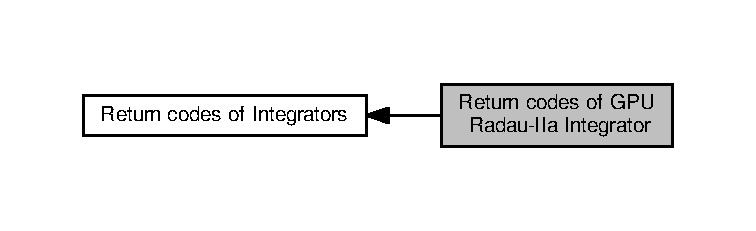
\includegraphics[width=350pt]{group__RKCU__ErrCodes}
\end{center}
\end{figure}
\subsection*{Macros}
\begin{DoxyCompactItemize}
\item 
\#define \hyperlink{group__RKCU__ErrCodes_gabd83bc0f9f475a2189a4db4a08b790ca}{E\+C\+\_\+success}~(0)
\begin{DoxyCompactList}\small\item\em Successful time step. \end{DoxyCompactList}\item 
\#define \hyperlink{group__RKCU__ErrCodes_gae0287841c08f86f5709660fd731615ad}{E\+C\+\_\+consecutive\+\_\+steps}~(1)
\begin{DoxyCompactList}\small\item\em Maximum number of consecutive internal timesteps with error reached. \end{DoxyCompactList}\item 
\#define \hyperlink{group__RKCU__ErrCodes_ga0f0275d9851ab5c19b79a963d5084df3}{E\+C\+\_\+max\+\_\+steps\+\_\+exceeded}~(2)
\begin{DoxyCompactList}\small\item\em Maximum number of internal timesteps exceeded. \end{DoxyCompactList}\item 
\#define \hyperlink{group__RKCU__ErrCodes_ga9326efd544880e2683c4453365ca2704}{E\+C\+\_\+h\+\_\+plus\+\_\+t\+\_\+equals\+\_\+h}~(3)
\begin{DoxyCompactList}\small\item\em Timescale reduced such that t + h == t in floating point math. \end{DoxyCompactList}\item 
\#define \hyperlink{group__RKCU__ErrCodes_gaae2906abd9ae8a2791c2e8626ca73a32}{E\+C\+\_\+newton\+\_\+max\+\_\+iterations\+\_\+exceeded}~(4)
\begin{DoxyCompactList}\small\item\em Maximum allowed Newton Iteration steps exceeded. \end{DoxyCompactList}\end{DoxyCompactItemize}


\subsection{Detailed Description}


\subsection{Macro Definition Documentation}
\index{Return codes of G\+P\+U Radau-\/\+I\+Ia Integrator@{Return codes of G\+P\+U Radau-\/\+I\+Ia Integrator}!E\+C\+\_\+consecutive\+\_\+steps@{E\+C\+\_\+consecutive\+\_\+steps}}
\index{E\+C\+\_\+consecutive\+\_\+steps@{E\+C\+\_\+consecutive\+\_\+steps}!Return codes of G\+P\+U Radau-\/\+I\+Ia Integrator@{Return codes of G\+P\+U Radau-\/\+I\+Ia Integrator}}
\subsubsection[{\texorpdfstring{E\+C\+\_\+consecutive\+\_\+steps}{EC_consecutive_steps}}]{\setlength{\rightskip}{0pt plus 5cm}\#define E\+C\+\_\+consecutive\+\_\+steps~(1)}\hypertarget{group__RKCU__ErrCodes_gae0287841c08f86f5709660fd731615ad}{}\label{group__RKCU__ErrCodes_gae0287841c08f86f5709660fd731615ad}


Maximum number of consecutive internal timesteps with error reached. 

\begin{DoxySeeAlso}{See also}
\hyperlink{radau2a_8cu_a172b5bc0830959ab49ca7cb9f0ae44bf}{Max\+\_\+consecutive\+\_\+errs} 
\end{DoxySeeAlso}
\index{Return codes of G\+P\+U Radau-\/\+I\+Ia Integrator@{Return codes of G\+P\+U Radau-\/\+I\+Ia Integrator}!E\+C\+\_\+h\+\_\+plus\+\_\+t\+\_\+equals\+\_\+h@{E\+C\+\_\+h\+\_\+plus\+\_\+t\+\_\+equals\+\_\+h}}
\index{E\+C\+\_\+h\+\_\+plus\+\_\+t\+\_\+equals\+\_\+h@{E\+C\+\_\+h\+\_\+plus\+\_\+t\+\_\+equals\+\_\+h}!Return codes of G\+P\+U Radau-\/\+I\+Ia Integrator@{Return codes of G\+P\+U Radau-\/\+I\+Ia Integrator}}
\subsubsection[{\texorpdfstring{E\+C\+\_\+h\+\_\+plus\+\_\+t\+\_\+equals\+\_\+h}{EC_h_plus_t_equals_h}}]{\setlength{\rightskip}{0pt plus 5cm}\#define E\+C\+\_\+h\+\_\+plus\+\_\+t\+\_\+equals\+\_\+h~(3)}\hypertarget{group__RKCU__ErrCodes_ga9326efd544880e2683c4453365ca2704}{}\label{group__RKCU__ErrCodes_ga9326efd544880e2683c4453365ca2704}


Timescale reduced such that t + h == t in floating point math. 

\index{Return codes of G\+P\+U Radau-\/\+I\+Ia Integrator@{Return codes of G\+P\+U Radau-\/\+I\+Ia Integrator}!E\+C\+\_\+max\+\_\+steps\+\_\+exceeded@{E\+C\+\_\+max\+\_\+steps\+\_\+exceeded}}
\index{E\+C\+\_\+max\+\_\+steps\+\_\+exceeded@{E\+C\+\_\+max\+\_\+steps\+\_\+exceeded}!Return codes of G\+P\+U Radau-\/\+I\+Ia Integrator@{Return codes of G\+P\+U Radau-\/\+I\+Ia Integrator}}
\subsubsection[{\texorpdfstring{E\+C\+\_\+max\+\_\+steps\+\_\+exceeded}{EC_max_steps_exceeded}}]{\setlength{\rightskip}{0pt plus 5cm}\#define E\+C\+\_\+max\+\_\+steps\+\_\+exceeded~(2)}\hypertarget{group__RKCU__ErrCodes_ga0f0275d9851ab5c19b79a963d5084df3}{}\label{group__RKCU__ErrCodes_ga0f0275d9851ab5c19b79a963d5084df3}


Maximum number of internal timesteps exceeded. 

\begin{DoxySeeAlso}{See also}
\hyperlink{radau2a_8cu_a4f5652e996f678da1b1b93c8aa4a7961}{Max\+\_\+no\+\_\+steps} 
\end{DoxySeeAlso}
\index{Return codes of G\+P\+U Radau-\/\+I\+Ia Integrator@{Return codes of G\+P\+U Radau-\/\+I\+Ia Integrator}!E\+C\+\_\+newton\+\_\+max\+\_\+iterations\+\_\+exceeded@{E\+C\+\_\+newton\+\_\+max\+\_\+iterations\+\_\+exceeded}}
\index{E\+C\+\_\+newton\+\_\+max\+\_\+iterations\+\_\+exceeded@{E\+C\+\_\+newton\+\_\+max\+\_\+iterations\+\_\+exceeded}!Return codes of G\+P\+U Radau-\/\+I\+Ia Integrator@{Return codes of G\+P\+U Radau-\/\+I\+Ia Integrator}}
\subsubsection[{\texorpdfstring{E\+C\+\_\+newton\+\_\+max\+\_\+iterations\+\_\+exceeded}{EC_newton_max_iterations_exceeded}}]{\setlength{\rightskip}{0pt plus 5cm}\#define E\+C\+\_\+newton\+\_\+max\+\_\+iterations\+\_\+exceeded~(4)}\hypertarget{group__RKCU__ErrCodes_gaae2906abd9ae8a2791c2e8626ca73a32}{}\label{group__RKCU__ErrCodes_gaae2906abd9ae8a2791c2e8626ca73a32}


Maximum allowed Newton Iteration steps exceeded. 

\begin{DoxySeeAlso}{See also}
\hyperlink{radau2a_8cu_ab408861ee5149b85ac129cb8a3875743}{Newton\+Maxit} 
\end{DoxySeeAlso}
\index{Return codes of G\+P\+U Radau-\/\+I\+Ia Integrator@{Return codes of G\+P\+U Radau-\/\+I\+Ia Integrator}!E\+C\+\_\+success@{E\+C\+\_\+success}}
\index{E\+C\+\_\+success@{E\+C\+\_\+success}!Return codes of G\+P\+U Radau-\/\+I\+Ia Integrator@{Return codes of G\+P\+U Radau-\/\+I\+Ia Integrator}}
\subsubsection[{\texorpdfstring{E\+C\+\_\+success}{EC_success}}]{\setlength{\rightskip}{0pt plus 5cm}\#define E\+C\+\_\+success~(0)}\hypertarget{group__RKCU__ErrCodes_gabd83bc0f9f475a2189a4db4a08b790ca}{}\label{group__RKCU__ErrCodes_gabd83bc0f9f475a2189a4db4a08b790ca}


Successful time step. 


\hypertarget{group__RK__ErrCodes}{}\section{Return codes of Radau-\/\+I\+Ia integrator}
\label{group__RK__ErrCodes}\index{Return codes of Radau-\/\+I\+Ia integrator@{Return codes of Radau-\/\+I\+Ia integrator}}
Collaboration diagram for Return codes of Radau-\/\+I\+Ia integrator\+:\nopagebreak
\begin{figure}[H]
\begin{center}
\leavevmode
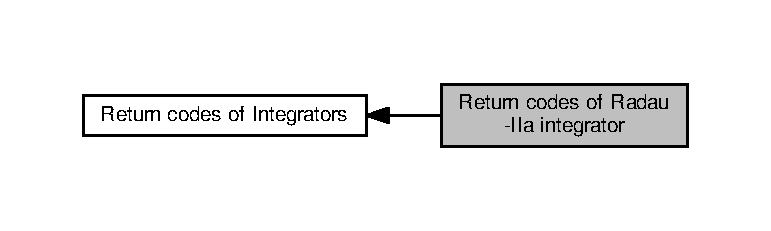
\includegraphics[width=350pt]{group__RK__ErrCodes}
\end{center}
\end{figure}
\subsection*{Macros}
\begin{DoxyCompactItemize}
\item 
\#define \hyperlink{group__RK__ErrCodes_gabd83bc0f9f475a2189a4db4a08b790ca}{E\+C\+\_\+success}~(0)
\begin{DoxyCompactList}\small\item\em Successful time step. \end{DoxyCompactList}\item 
\#define \hyperlink{group__RK__ErrCodes_gae0287841c08f86f5709660fd731615ad}{E\+C\+\_\+consecutive\+\_\+steps}~(1)
\begin{DoxyCompactList}\small\item\em Maximum number of consecutive internal timesteps with error reached. \end{DoxyCompactList}\item 
\#define \hyperlink{group__RK__ErrCodes_ga0f0275d9851ab5c19b79a963d5084df3}{E\+C\+\_\+max\+\_\+steps\+\_\+exceeded}~(2)
\begin{DoxyCompactList}\small\item\em Maximum number of internal timesteps exceeded. \end{DoxyCompactList}\item 
\#define \hyperlink{group__RK__ErrCodes_ga9326efd544880e2683c4453365ca2704}{E\+C\+\_\+h\+\_\+plus\+\_\+t\+\_\+equals\+\_\+h}~(3)
\begin{DoxyCompactList}\small\item\em Timescale reduced such that t + h == t in floating point math. \end{DoxyCompactList}\item 
\#define \hyperlink{group__RK__ErrCodes_gaae2906abd9ae8a2791c2e8626ca73a32}{E\+C\+\_\+newton\+\_\+max\+\_\+iterations\+\_\+exceeded}~(4)
\begin{DoxyCompactList}\small\item\em Maximum allowed Newton Iteration steps exceeded. \end{DoxyCompactList}\end{DoxyCompactItemize}


\subsection{Detailed Description}


\subsection{Macro Definition Documentation}
\index{Return codes of Radau-\/\+I\+Ia integrator@{Return codes of Radau-\/\+I\+Ia integrator}!E\+C\+\_\+consecutive\+\_\+steps@{E\+C\+\_\+consecutive\+\_\+steps}}
\index{E\+C\+\_\+consecutive\+\_\+steps@{E\+C\+\_\+consecutive\+\_\+steps}!Return codes of Radau-\/\+I\+Ia integrator@{Return codes of Radau-\/\+I\+Ia integrator}}
\subsubsection[{\texorpdfstring{E\+C\+\_\+consecutive\+\_\+steps}{EC_consecutive_steps}}]{\setlength{\rightskip}{0pt plus 5cm}\#define E\+C\+\_\+consecutive\+\_\+steps~(1)}\hypertarget{group__RK__ErrCodes_gae0287841c08f86f5709660fd731615ad}{}\label{group__RK__ErrCodes_gae0287841c08f86f5709660fd731615ad}


Maximum number of consecutive internal timesteps with error reached. 

\begin{DoxySeeAlso}{See also}
\hyperlink{radau2a_8cu_a172b5bc0830959ab49ca7cb9f0ae44bf}{Max\+\_\+consecutive\+\_\+errs} 
\end{DoxySeeAlso}
\index{Return codes of Radau-\/\+I\+Ia integrator@{Return codes of Radau-\/\+I\+Ia integrator}!E\+C\+\_\+h\+\_\+plus\+\_\+t\+\_\+equals\+\_\+h@{E\+C\+\_\+h\+\_\+plus\+\_\+t\+\_\+equals\+\_\+h}}
\index{E\+C\+\_\+h\+\_\+plus\+\_\+t\+\_\+equals\+\_\+h@{E\+C\+\_\+h\+\_\+plus\+\_\+t\+\_\+equals\+\_\+h}!Return codes of Radau-\/\+I\+Ia integrator@{Return codes of Radau-\/\+I\+Ia integrator}}
\subsubsection[{\texorpdfstring{E\+C\+\_\+h\+\_\+plus\+\_\+t\+\_\+equals\+\_\+h}{EC_h_plus_t_equals_h}}]{\setlength{\rightskip}{0pt plus 5cm}\#define E\+C\+\_\+h\+\_\+plus\+\_\+t\+\_\+equals\+\_\+h~(3)}\hypertarget{group__RK__ErrCodes_ga9326efd544880e2683c4453365ca2704}{}\label{group__RK__ErrCodes_ga9326efd544880e2683c4453365ca2704}


Timescale reduced such that t + h == t in floating point math. 

\index{Return codes of Radau-\/\+I\+Ia integrator@{Return codes of Radau-\/\+I\+Ia integrator}!E\+C\+\_\+max\+\_\+steps\+\_\+exceeded@{E\+C\+\_\+max\+\_\+steps\+\_\+exceeded}}
\index{E\+C\+\_\+max\+\_\+steps\+\_\+exceeded@{E\+C\+\_\+max\+\_\+steps\+\_\+exceeded}!Return codes of Radau-\/\+I\+Ia integrator@{Return codes of Radau-\/\+I\+Ia integrator}}
\subsubsection[{\texorpdfstring{E\+C\+\_\+max\+\_\+steps\+\_\+exceeded}{EC_max_steps_exceeded}}]{\setlength{\rightskip}{0pt plus 5cm}\#define E\+C\+\_\+max\+\_\+steps\+\_\+exceeded~(2)}\hypertarget{group__RK__ErrCodes_ga0f0275d9851ab5c19b79a963d5084df3}{}\label{group__RK__ErrCodes_ga0f0275d9851ab5c19b79a963d5084df3}


Maximum number of internal timesteps exceeded. 

\begin{DoxySeeAlso}{See also}
\hyperlink{radau2a_8cu_a4f5652e996f678da1b1b93c8aa4a7961}{Max\+\_\+no\+\_\+steps} 
\end{DoxySeeAlso}
\index{Return codes of Radau-\/\+I\+Ia integrator@{Return codes of Radau-\/\+I\+Ia integrator}!E\+C\+\_\+newton\+\_\+max\+\_\+iterations\+\_\+exceeded@{E\+C\+\_\+newton\+\_\+max\+\_\+iterations\+\_\+exceeded}}
\index{E\+C\+\_\+newton\+\_\+max\+\_\+iterations\+\_\+exceeded@{E\+C\+\_\+newton\+\_\+max\+\_\+iterations\+\_\+exceeded}!Return codes of Radau-\/\+I\+Ia integrator@{Return codes of Radau-\/\+I\+Ia integrator}}
\subsubsection[{\texorpdfstring{E\+C\+\_\+newton\+\_\+max\+\_\+iterations\+\_\+exceeded}{EC_newton_max_iterations_exceeded}}]{\setlength{\rightskip}{0pt plus 5cm}\#define E\+C\+\_\+newton\+\_\+max\+\_\+iterations\+\_\+exceeded~(4)}\hypertarget{group__RK__ErrCodes_gaae2906abd9ae8a2791c2e8626ca73a32}{}\label{group__RK__ErrCodes_gaae2906abd9ae8a2791c2e8626ca73a32}


Maximum allowed Newton Iteration steps exceeded. 

\begin{DoxySeeAlso}{See also}
\hyperlink{radau2a_8cu_ab408861ee5149b85ac129cb8a3875743}{Newton\+Maxit} 
\end{DoxySeeAlso}
\index{Return codes of Radau-\/\+I\+Ia integrator@{Return codes of Radau-\/\+I\+Ia integrator}!E\+C\+\_\+success@{E\+C\+\_\+success}}
\index{E\+C\+\_\+success@{E\+C\+\_\+success}!Return codes of Radau-\/\+I\+Ia integrator@{Return codes of Radau-\/\+I\+Ia integrator}}
\subsubsection[{\texorpdfstring{E\+C\+\_\+success}{EC_success}}]{\setlength{\rightskip}{0pt plus 5cm}\#define E\+C\+\_\+success~(0)}\hypertarget{group__RK__ErrCodes_gabd83bc0f9f475a2189a4db4a08b790ca}{}\label{group__RK__ErrCodes_gabd83bc0f9f475a2189a4db4a08b790ca}


Successful time step. 


\hypertarget{group__exp4cu__ErrCodes}{}\section{Return codes of G\+PU E\+X\+P\+R\+B43 integrator}
\label{group__exp4cu__ErrCodes}\index{Return codes of G\+P\+U E\+X\+P\+R\+B43 integrator@{Return codes of G\+P\+U E\+X\+P\+R\+B43 integrator}}
Collaboration diagram for Return codes of G\+PU E\+X\+P\+R\+B43 integrator\+:
\nopagebreak
\begin{figure}[H]
\begin{center}
\leavevmode
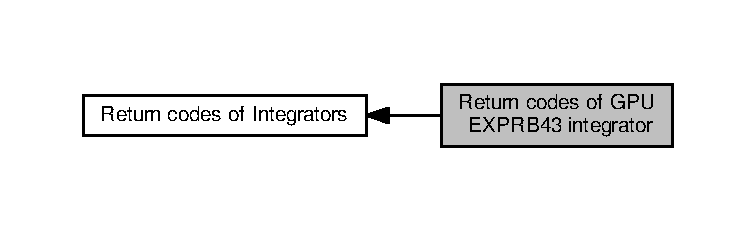
\includegraphics[width=350pt]{group__exp4cu__ErrCodes}
\end{center}
\end{figure}
\subsection*{Macros}
\begin{DoxyCompactItemize}
\item 
\#define \hyperlink{group__exp4cu__ErrCodes_gabd83bc0f9f475a2189a4db4a08b790ca}{E\+C\+\_\+success}~(0)
\begin{DoxyCompactList}\small\item\em Successful integration step. \end{DoxyCompactList}\item 
\#define \hyperlink{group__exp4cu__ErrCodes_gae0287841c08f86f5709660fd731615ad}{E\+C\+\_\+consecutive\+\_\+steps}~(1)
\begin{DoxyCompactList}\small\item\em Maximum consecutive errors on internal integration steps reached. \end{DoxyCompactList}\item 
\#define \hyperlink{group__exp4cu__ErrCodes_ga0f0275d9851ab5c19b79a963d5084df3}{E\+C\+\_\+max\+\_\+steps\+\_\+exceeded}~(2)
\begin{DoxyCompactList}\small\item\em Maximum number of internal integration steps reached. \end{DoxyCompactList}\item 
\#define \hyperlink{group__exp4cu__ErrCodes_ga9326efd544880e2683c4453365ca2704}{E\+C\+\_\+h\+\_\+plus\+\_\+t\+\_\+equals\+\_\+h}~(3)
\begin{DoxyCompactList}\small\item\em Timestep reduced such that update would have no effect on simulation time. \end{DoxyCompactList}\end{DoxyCompactItemize}


\subsection{Detailed Description}


\subsection{Macro Definition Documentation}
\index{Return codes of G\+P\+U E\+X\+P\+R\+B43 integrator@{Return codes of G\+P\+U E\+X\+P\+R\+B43 integrator}!E\+C\+\_\+consecutive\+\_\+steps@{E\+C\+\_\+consecutive\+\_\+steps}}
\index{E\+C\+\_\+consecutive\+\_\+steps@{E\+C\+\_\+consecutive\+\_\+steps}!Return codes of G\+P\+U E\+X\+P\+R\+B43 integrator@{Return codes of G\+P\+U E\+X\+P\+R\+B43 integrator}}
\subsubsection[{\texorpdfstring{E\+C\+\_\+consecutive\+\_\+steps}{EC_consecutive_steps}}]{\setlength{\rightskip}{0pt plus 5cm}\#define E\+C\+\_\+consecutive\+\_\+steps~(1)}\hypertarget{group__exp4cu__ErrCodes_gae0287841c08f86f5709660fd731615ad}{}\label{group__exp4cu__ErrCodes_gae0287841c08f86f5709660fd731615ad}


Maximum consecutive errors on internal integration steps reached. 

\index{Return codes of G\+P\+U E\+X\+P\+R\+B43 integrator@{Return codes of G\+P\+U E\+X\+P\+R\+B43 integrator}!E\+C\+\_\+h\+\_\+plus\+\_\+t\+\_\+equals\+\_\+h@{E\+C\+\_\+h\+\_\+plus\+\_\+t\+\_\+equals\+\_\+h}}
\index{E\+C\+\_\+h\+\_\+plus\+\_\+t\+\_\+equals\+\_\+h@{E\+C\+\_\+h\+\_\+plus\+\_\+t\+\_\+equals\+\_\+h}!Return codes of G\+P\+U E\+X\+P\+R\+B43 integrator@{Return codes of G\+P\+U E\+X\+P\+R\+B43 integrator}}
\subsubsection[{\texorpdfstring{E\+C\+\_\+h\+\_\+plus\+\_\+t\+\_\+equals\+\_\+h}{EC_h_plus_t_equals_h}}]{\setlength{\rightskip}{0pt plus 5cm}\#define E\+C\+\_\+h\+\_\+plus\+\_\+t\+\_\+equals\+\_\+h~(3)}\hypertarget{group__exp4cu__ErrCodes_ga9326efd544880e2683c4453365ca2704}{}\label{group__exp4cu__ErrCodes_ga9326efd544880e2683c4453365ca2704}


Timestep reduced such that update would have no effect on simulation time. 

\index{Return codes of G\+P\+U E\+X\+P\+R\+B43 integrator@{Return codes of G\+P\+U E\+X\+P\+R\+B43 integrator}!E\+C\+\_\+max\+\_\+steps\+\_\+exceeded@{E\+C\+\_\+max\+\_\+steps\+\_\+exceeded}}
\index{E\+C\+\_\+max\+\_\+steps\+\_\+exceeded@{E\+C\+\_\+max\+\_\+steps\+\_\+exceeded}!Return codes of G\+P\+U E\+X\+P\+R\+B43 integrator@{Return codes of G\+P\+U E\+X\+P\+R\+B43 integrator}}
\subsubsection[{\texorpdfstring{E\+C\+\_\+max\+\_\+steps\+\_\+exceeded}{EC_max_steps_exceeded}}]{\setlength{\rightskip}{0pt plus 5cm}\#define E\+C\+\_\+max\+\_\+steps\+\_\+exceeded~(2)}\hypertarget{group__exp4cu__ErrCodes_ga0f0275d9851ab5c19b79a963d5084df3}{}\label{group__exp4cu__ErrCodes_ga0f0275d9851ab5c19b79a963d5084df3}


Maximum number of internal integration steps reached. 

\index{Return codes of G\+P\+U E\+X\+P\+R\+B43 integrator@{Return codes of G\+P\+U E\+X\+P\+R\+B43 integrator}!E\+C\+\_\+success@{E\+C\+\_\+success}}
\index{E\+C\+\_\+success@{E\+C\+\_\+success}!Return codes of G\+P\+U E\+X\+P\+R\+B43 integrator@{Return codes of G\+P\+U E\+X\+P\+R\+B43 integrator}}
\subsubsection[{\texorpdfstring{E\+C\+\_\+success}{EC_success}}]{\setlength{\rightskip}{0pt plus 5cm}\#define E\+C\+\_\+success~(0)}\hypertarget{group__exp4cu__ErrCodes_gabd83bc0f9f475a2189a4db4a08b790ca}{}\label{group__exp4cu__ErrCodes_gabd83bc0f9f475a2189a4db4a08b790ca}


Successful integration step. 


\hypertarget{group__exp4__ErrCodes}{}\section{Return codes of E\+X\+P4 integrator}
\label{group__exp4__ErrCodes}\index{Return codes of E\+X\+P4 integrator@{Return codes of E\+X\+P4 integrator}}
\subsection*{Macros}
\begin{DoxyCompactItemize}
\item 
\#define \hyperlink{group__exp4__ErrCodes_gabd83bc0f9f475a2189a4db4a08b790ca}{E\+C\+\_\+success}~(0)
\begin{DoxyCompactList}\small\item\em Successful integration step. \end{DoxyCompactList}\item 
\#define \hyperlink{group__exp4__ErrCodes_gae0287841c08f86f5709660fd731615ad}{E\+C\+\_\+consecutive\+\_\+steps}~(1)
\begin{DoxyCompactList}\small\item\em Maximum consecutive errors on internal integration steps reached. \end{DoxyCompactList}\item 
\#define \hyperlink{group__exp4__ErrCodes_ga0f0275d9851ab5c19b79a963d5084df3}{E\+C\+\_\+max\+\_\+steps\+\_\+exceeded}~(2)
\begin{DoxyCompactList}\small\item\em Maximum number of internal integration steps reached. \end{DoxyCompactList}\item 
\#define \hyperlink{group__exp4__ErrCodes_ga9326efd544880e2683c4453365ca2704}{E\+C\+\_\+h\+\_\+plus\+\_\+t\+\_\+equals\+\_\+h}~(3)
\begin{DoxyCompactList}\small\item\em Timestep reduced such that update would have no effect on simulation time. \end{DoxyCompactList}\end{DoxyCompactItemize}


\subsection{Detailed Description}


\subsection{Macro Definition Documentation}
\index{Return codes of E\+X\+P4 integrator@{Return codes of E\+X\+P4 integrator}!E\+C\+\_\+consecutive\+\_\+steps@{E\+C\+\_\+consecutive\+\_\+steps}}
\index{E\+C\+\_\+consecutive\+\_\+steps@{E\+C\+\_\+consecutive\+\_\+steps}!Return codes of E\+X\+P4 integrator@{Return codes of E\+X\+P4 integrator}}
\subsubsection[{\texorpdfstring{E\+C\+\_\+consecutive\+\_\+steps}{EC_consecutive_steps}}]{\setlength{\rightskip}{0pt plus 5cm}\#define E\+C\+\_\+consecutive\+\_\+steps~(1)}\hypertarget{group__exp4__ErrCodes_gae0287841c08f86f5709660fd731615ad}{}\label{group__exp4__ErrCodes_gae0287841c08f86f5709660fd731615ad}


Maximum consecutive errors on internal integration steps reached. 

\index{Return codes of E\+X\+P4 integrator@{Return codes of E\+X\+P4 integrator}!E\+C\+\_\+h\+\_\+plus\+\_\+t\+\_\+equals\+\_\+h@{E\+C\+\_\+h\+\_\+plus\+\_\+t\+\_\+equals\+\_\+h}}
\index{E\+C\+\_\+h\+\_\+plus\+\_\+t\+\_\+equals\+\_\+h@{E\+C\+\_\+h\+\_\+plus\+\_\+t\+\_\+equals\+\_\+h}!Return codes of E\+X\+P4 integrator@{Return codes of E\+X\+P4 integrator}}
\subsubsection[{\texorpdfstring{E\+C\+\_\+h\+\_\+plus\+\_\+t\+\_\+equals\+\_\+h}{EC_h_plus_t_equals_h}}]{\setlength{\rightskip}{0pt plus 5cm}\#define E\+C\+\_\+h\+\_\+plus\+\_\+t\+\_\+equals\+\_\+h~(3)}\hypertarget{group__exp4__ErrCodes_ga9326efd544880e2683c4453365ca2704}{}\label{group__exp4__ErrCodes_ga9326efd544880e2683c4453365ca2704}


Timestep reduced such that update would have no effect on simulation time. 

\index{Return codes of E\+X\+P4 integrator@{Return codes of E\+X\+P4 integrator}!E\+C\+\_\+max\+\_\+steps\+\_\+exceeded@{E\+C\+\_\+max\+\_\+steps\+\_\+exceeded}}
\index{E\+C\+\_\+max\+\_\+steps\+\_\+exceeded@{E\+C\+\_\+max\+\_\+steps\+\_\+exceeded}!Return codes of E\+X\+P4 integrator@{Return codes of E\+X\+P4 integrator}}
\subsubsection[{\texorpdfstring{E\+C\+\_\+max\+\_\+steps\+\_\+exceeded}{EC_max_steps_exceeded}}]{\setlength{\rightskip}{0pt plus 5cm}\#define E\+C\+\_\+max\+\_\+steps\+\_\+exceeded~(2)}\hypertarget{group__exp4__ErrCodes_ga0f0275d9851ab5c19b79a963d5084df3}{}\label{group__exp4__ErrCodes_ga0f0275d9851ab5c19b79a963d5084df3}


Maximum number of internal integration steps reached. 

\index{Return codes of E\+X\+P4 integrator@{Return codes of E\+X\+P4 integrator}!E\+C\+\_\+success@{E\+C\+\_\+success}}
\index{E\+C\+\_\+success@{E\+C\+\_\+success}!Return codes of E\+X\+P4 integrator@{Return codes of E\+X\+P4 integrator}}
\subsubsection[{\texorpdfstring{E\+C\+\_\+success}{EC_success}}]{\setlength{\rightskip}{0pt plus 5cm}\#define E\+C\+\_\+success~(0)}\hypertarget{group__exp4__ErrCodes_gabd83bc0f9f475a2189a4db4a08b790ca}{}\label{group__exp4__ErrCodes_gabd83bc0f9f475a2189a4db4a08b790ca}


Successful integration step. 


\hypertarget{group__exprb43cu__ErrCodes}{}\section{Return codes of G\+PU E\+X\+P4 integrator}
\label{group__exprb43cu__ErrCodes}\index{Return codes of G\+P\+U E\+X\+P4 integrator@{Return codes of G\+P\+U E\+X\+P4 integrator}}
\subsection*{Macros}
\begin{DoxyCompactItemize}
\item 
\#define \hyperlink{group__exprb43cu__ErrCodes_gabd83bc0f9f475a2189a4db4a08b790ca}{E\+C\+\_\+success}~(0)
\begin{DoxyCompactList}\small\item\em Successful integration step. \end{DoxyCompactList}\item 
\#define \hyperlink{group__exprb43cu__ErrCodes_gae0287841c08f86f5709660fd731615ad}{E\+C\+\_\+consecutive\+\_\+steps}~(1)
\begin{DoxyCompactList}\small\item\em Maximum consecutive errors on internal integration steps reached. \end{DoxyCompactList}\item 
\#define \hyperlink{group__exprb43cu__ErrCodes_ga0f0275d9851ab5c19b79a963d5084df3}{E\+C\+\_\+max\+\_\+steps\+\_\+exceeded}~(2)
\begin{DoxyCompactList}\small\item\em Maximum number of internal integration steps reached. \end{DoxyCompactList}\item 
\#define \hyperlink{group__exprb43cu__ErrCodes_ga9326efd544880e2683c4453365ca2704}{E\+C\+\_\+h\+\_\+plus\+\_\+t\+\_\+equals\+\_\+h}~(3)
\begin{DoxyCompactList}\small\item\em Timestep reduced such that update would have no effect on simulation time. \end{DoxyCompactList}\end{DoxyCompactItemize}


\subsection{Detailed Description}


\subsection{Macro Definition Documentation}
\index{Return codes of G\+P\+U E\+X\+P4 integrator@{Return codes of G\+P\+U E\+X\+P4 integrator}!E\+C\+\_\+consecutive\+\_\+steps@{E\+C\+\_\+consecutive\+\_\+steps}}
\index{E\+C\+\_\+consecutive\+\_\+steps@{E\+C\+\_\+consecutive\+\_\+steps}!Return codes of G\+P\+U E\+X\+P4 integrator@{Return codes of G\+P\+U E\+X\+P4 integrator}}
\subsubsection[{\texorpdfstring{E\+C\+\_\+consecutive\+\_\+steps}{EC_consecutive_steps}}]{\setlength{\rightskip}{0pt plus 5cm}\#define E\+C\+\_\+consecutive\+\_\+steps~(1)}\hypertarget{group__exprb43cu__ErrCodes_gae0287841c08f86f5709660fd731615ad}{}\label{group__exprb43cu__ErrCodes_gae0287841c08f86f5709660fd731615ad}


Maximum consecutive errors on internal integration steps reached. 

\index{Return codes of G\+P\+U E\+X\+P4 integrator@{Return codes of G\+P\+U E\+X\+P4 integrator}!E\+C\+\_\+h\+\_\+plus\+\_\+t\+\_\+equals\+\_\+h@{E\+C\+\_\+h\+\_\+plus\+\_\+t\+\_\+equals\+\_\+h}}
\index{E\+C\+\_\+h\+\_\+plus\+\_\+t\+\_\+equals\+\_\+h@{E\+C\+\_\+h\+\_\+plus\+\_\+t\+\_\+equals\+\_\+h}!Return codes of G\+P\+U E\+X\+P4 integrator@{Return codes of G\+P\+U E\+X\+P4 integrator}}
\subsubsection[{\texorpdfstring{E\+C\+\_\+h\+\_\+plus\+\_\+t\+\_\+equals\+\_\+h}{EC_h_plus_t_equals_h}}]{\setlength{\rightskip}{0pt plus 5cm}\#define E\+C\+\_\+h\+\_\+plus\+\_\+t\+\_\+equals\+\_\+h~(3)}\hypertarget{group__exprb43cu__ErrCodes_ga9326efd544880e2683c4453365ca2704}{}\label{group__exprb43cu__ErrCodes_ga9326efd544880e2683c4453365ca2704}


Timestep reduced such that update would have no effect on simulation time. 

\index{Return codes of G\+P\+U E\+X\+P4 integrator@{Return codes of G\+P\+U E\+X\+P4 integrator}!E\+C\+\_\+max\+\_\+steps\+\_\+exceeded@{E\+C\+\_\+max\+\_\+steps\+\_\+exceeded}}
\index{E\+C\+\_\+max\+\_\+steps\+\_\+exceeded@{E\+C\+\_\+max\+\_\+steps\+\_\+exceeded}!Return codes of G\+P\+U E\+X\+P4 integrator@{Return codes of G\+P\+U E\+X\+P4 integrator}}
\subsubsection[{\texorpdfstring{E\+C\+\_\+max\+\_\+steps\+\_\+exceeded}{EC_max_steps_exceeded}}]{\setlength{\rightskip}{0pt plus 5cm}\#define E\+C\+\_\+max\+\_\+steps\+\_\+exceeded~(2)}\hypertarget{group__exprb43cu__ErrCodes_ga0f0275d9851ab5c19b79a963d5084df3}{}\label{group__exprb43cu__ErrCodes_ga0f0275d9851ab5c19b79a963d5084df3}


Maximum number of internal integration steps reached. 

\index{Return codes of G\+P\+U E\+X\+P4 integrator@{Return codes of G\+P\+U E\+X\+P4 integrator}!E\+C\+\_\+success@{E\+C\+\_\+success}}
\index{E\+C\+\_\+success@{E\+C\+\_\+success}!Return codes of G\+P\+U E\+X\+P4 integrator@{Return codes of G\+P\+U E\+X\+P4 integrator}}
\subsubsection[{\texorpdfstring{E\+C\+\_\+success}{EC_success}}]{\setlength{\rightskip}{0pt plus 5cm}\#define E\+C\+\_\+success~(0)}\hypertarget{group__exprb43cu__ErrCodes_gabd83bc0f9f475a2189a4db4a08b790ca}{}\label{group__exprb43cu__ErrCodes_gabd83bc0f9f475a2189a4db4a08b790ca}


Successful integration step. 


\hypertarget{group__exprb43__ErrCodes}{}\section{Return codes of E\+X\+P\+R\+B43 integrator}
\label{group__exprb43__ErrCodes}\index{Return codes of E\+X\+P\+R\+B43 integrator@{Return codes of E\+X\+P\+R\+B43 integrator}}
Collaboration diagram for Return codes of E\+X\+P\+R\+B43 integrator\+:
\nopagebreak
\begin{figure}[H]
\begin{center}
\leavevmode
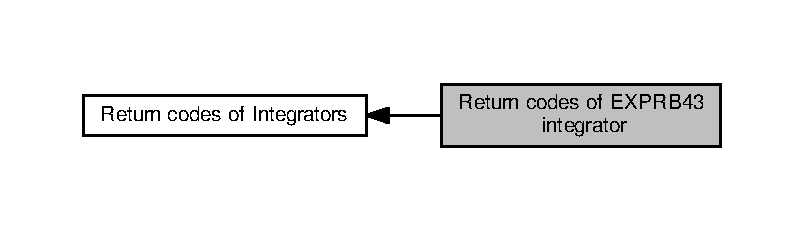
\includegraphics[width=350pt]{group__exprb43__ErrCodes}
\end{center}
\end{figure}
\subsection*{Macros}
\begin{DoxyCompactItemize}
\item 
\#define \hyperlink{group__exprb43__ErrCodes_gabd83bc0f9f475a2189a4db4a08b790ca}{E\+C\+\_\+success}~(0)
\begin{DoxyCompactList}\small\item\em Successful integration step. \end{DoxyCompactList}\item 
\#define \hyperlink{group__exprb43__ErrCodes_gae0287841c08f86f5709660fd731615ad}{E\+C\+\_\+consecutive\+\_\+steps}~(1)
\begin{DoxyCompactList}\small\item\em Maximum consecutive errors on internal integration steps reached. \end{DoxyCompactList}\item 
\#define \hyperlink{group__exprb43__ErrCodes_ga0f0275d9851ab5c19b79a963d5084df3}{E\+C\+\_\+max\+\_\+steps\+\_\+exceeded}~(2)
\begin{DoxyCompactList}\small\item\em Maximum number of internal integration steps reached. \end{DoxyCompactList}\item 
\#define \hyperlink{group__exprb43__ErrCodes_ga9326efd544880e2683c4453365ca2704}{E\+C\+\_\+h\+\_\+plus\+\_\+t\+\_\+equals\+\_\+h}~(3)
\begin{DoxyCompactList}\small\item\em Timestep reduced such that update would have no effect on simulation time. \end{DoxyCompactList}\end{DoxyCompactItemize}


\subsection{Detailed Description}


\subsection{Macro Definition Documentation}
\index{Return codes of E\+X\+P\+R\+B43 integrator@{Return codes of E\+X\+P\+R\+B43 integrator}!E\+C\+\_\+consecutive\+\_\+steps@{E\+C\+\_\+consecutive\+\_\+steps}}
\index{E\+C\+\_\+consecutive\+\_\+steps@{E\+C\+\_\+consecutive\+\_\+steps}!Return codes of E\+X\+P\+R\+B43 integrator@{Return codes of E\+X\+P\+R\+B43 integrator}}
\subsubsection[{\texorpdfstring{E\+C\+\_\+consecutive\+\_\+steps}{EC_consecutive_steps}}]{\setlength{\rightskip}{0pt plus 5cm}\#define E\+C\+\_\+consecutive\+\_\+steps~(1)}\hypertarget{group__exprb43__ErrCodes_gae0287841c08f86f5709660fd731615ad}{}\label{group__exprb43__ErrCodes_gae0287841c08f86f5709660fd731615ad}


Maximum consecutive errors on internal integration steps reached. 

\index{Return codes of E\+X\+P\+R\+B43 integrator@{Return codes of E\+X\+P\+R\+B43 integrator}!E\+C\+\_\+h\+\_\+plus\+\_\+t\+\_\+equals\+\_\+h@{E\+C\+\_\+h\+\_\+plus\+\_\+t\+\_\+equals\+\_\+h}}
\index{E\+C\+\_\+h\+\_\+plus\+\_\+t\+\_\+equals\+\_\+h@{E\+C\+\_\+h\+\_\+plus\+\_\+t\+\_\+equals\+\_\+h}!Return codes of E\+X\+P\+R\+B43 integrator@{Return codes of E\+X\+P\+R\+B43 integrator}}
\subsubsection[{\texorpdfstring{E\+C\+\_\+h\+\_\+plus\+\_\+t\+\_\+equals\+\_\+h}{EC_h_plus_t_equals_h}}]{\setlength{\rightskip}{0pt plus 5cm}\#define E\+C\+\_\+h\+\_\+plus\+\_\+t\+\_\+equals\+\_\+h~(3)}\hypertarget{group__exprb43__ErrCodes_ga9326efd544880e2683c4453365ca2704}{}\label{group__exprb43__ErrCodes_ga9326efd544880e2683c4453365ca2704}


Timestep reduced such that update would have no effect on simulation time. 

\index{Return codes of E\+X\+P\+R\+B43 integrator@{Return codes of E\+X\+P\+R\+B43 integrator}!E\+C\+\_\+max\+\_\+steps\+\_\+exceeded@{E\+C\+\_\+max\+\_\+steps\+\_\+exceeded}}
\index{E\+C\+\_\+max\+\_\+steps\+\_\+exceeded@{E\+C\+\_\+max\+\_\+steps\+\_\+exceeded}!Return codes of E\+X\+P\+R\+B43 integrator@{Return codes of E\+X\+P\+R\+B43 integrator}}
\subsubsection[{\texorpdfstring{E\+C\+\_\+max\+\_\+steps\+\_\+exceeded}{EC_max_steps_exceeded}}]{\setlength{\rightskip}{0pt plus 5cm}\#define E\+C\+\_\+max\+\_\+steps\+\_\+exceeded~(2)}\hypertarget{group__exprb43__ErrCodes_ga0f0275d9851ab5c19b79a963d5084df3}{}\label{group__exprb43__ErrCodes_ga0f0275d9851ab5c19b79a963d5084df3}


Maximum number of internal integration steps reached. 

\index{Return codes of E\+X\+P\+R\+B43 integrator@{Return codes of E\+X\+P\+R\+B43 integrator}!E\+C\+\_\+success@{E\+C\+\_\+success}}
\index{E\+C\+\_\+success@{E\+C\+\_\+success}!Return codes of E\+X\+P\+R\+B43 integrator@{Return codes of E\+X\+P\+R\+B43 integrator}}
\subsubsection[{\texorpdfstring{E\+C\+\_\+success}{EC_success}}]{\setlength{\rightskip}{0pt plus 5cm}\#define E\+C\+\_\+success~(0)}\hypertarget{group__exprb43__ErrCodes_gabd83bc0f9f475a2189a4db4a08b790ca}{}\label{group__exprb43__ErrCodes_gabd83bc0f9f475a2189a4db4a08b790ca}


Successful integration step. 


\hypertarget{group__CUErrorCodes}{}\section{Return codes of Integrators}
\label{group__CUErrorCodes}\index{Return codes of Integrators@{Return codes of Integrators}}
Collaboration diagram for Return codes of Integrators\+:
\nopagebreak
\begin{figure}[H]
\begin{center}
\leavevmode
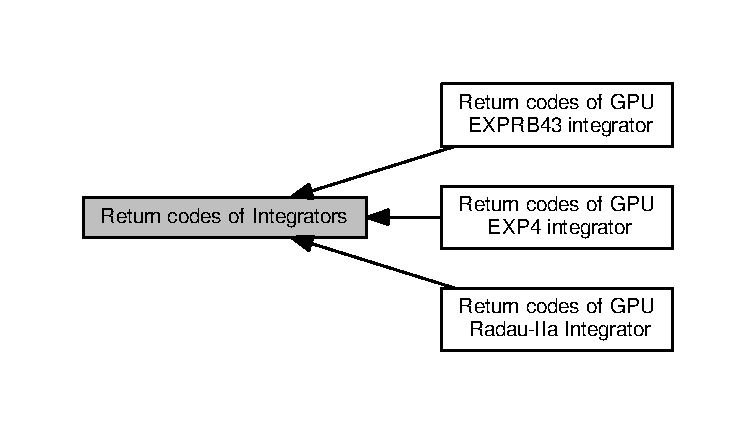
\includegraphics[width=350pt]{group__CUErrorCodes}
\end{center}
\end{figure}
\subsection*{Modules}
\begin{DoxyCompactItemize}
\item 
\hyperlink{group__RKCU__ErrCodes}{Return codes of G\+P\+U Radau-\/\+I\+Ia Integrator}
\item 
\hyperlink{group__exp4cu__ErrCodes}{Return codes of G\+P\+U E\+X\+P\+R\+B43 integrator}
\item 
\hyperlink{group__exprb43cu__ErrCodes}{Return codes of G\+P\+U E\+X\+P4 integrator}
\end{DoxyCompactItemize}


\subsection{Detailed Description}

\hypertarget{group__ErrorCodes}{}\section{Return codes of Integrators}
\label{group__ErrorCodes}\index{Return codes of Integrators@{Return codes of Integrators}}
Collaboration diagram for Return codes of Integrators\+:
\nopagebreak
\begin{figure}[H]
\begin{center}
\leavevmode
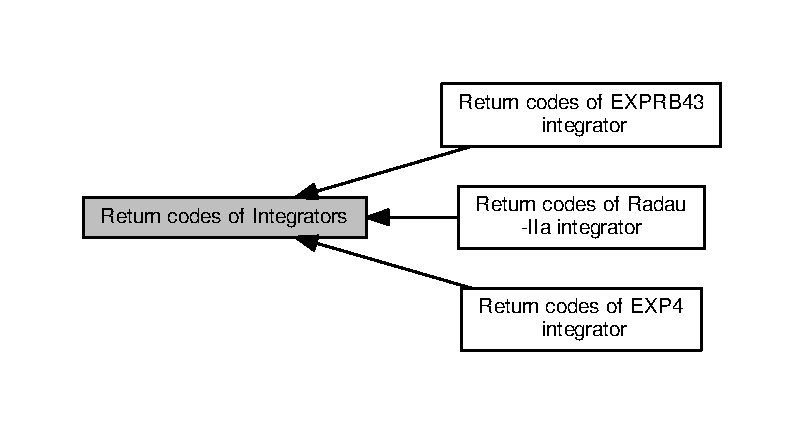
\includegraphics[width=350pt]{group__ErrorCodes}
\end{center}
\end{figure}
\subsection*{Modules}
\begin{DoxyCompactItemize}
\item 
\hyperlink{group__RK__ErrCodes}{Return codes of Radau-\/\+I\+Ia integrator}
\item 
\hyperlink{group__exp4__ErrCodes}{Return codes of E\+X\+P4 integrator}
\item 
\hyperlink{group__exprb43__ErrCodes}{Return codes of E\+X\+P\+R\+B43 integrator}
\end{DoxyCompactItemize}


\subsection{Detailed Description}

\chapter{Namespace Documentation}
\hypertarget{namespacecvode}{}\section{cvode Namespace Reference}
\label{namespacecvode}\index{cvode@{cvode}}
\subsection*{Functions}
\begin{DoxyCompactItemize}
\item 
int \hyperlink{namespacecvode_aa10a063b2a82d5b49c2bb338f16ddae4}{dydt\+\_\+cvodes} (double t, N\+\_\+\+Vector y, N\+\_\+\+Vector ydot, void $\ast$f)
\begin{DoxyCompactList}\small\item\em The C\+V\+O\+D\+Es R\+HS interface. \end{DoxyCompactList}\item 
int \hyperlink{namespacecvode_ab2efc395730d25bedc496a62e7896d24}{eval\+\_\+jacob\+\_\+cvodes} (long int N, double t, N\+\_\+\+Vector y, N\+\_\+\+Vector ydot, Dls\+Mat Jac, void $\ast$f, N\+\_\+\+Vector tmp1, N\+\_\+\+Vector tmp2, N\+\_\+\+Vector tmp3)
\begin{DoxyCompactList}\small\item\em The C\+V\+O\+D\+Es Jacobian interface for a direct dense Jacobian. \end{DoxyCompactList}\item 
void \hyperlink{namespacecvode_abe146525cea80d8032cd30b4441b5872}{initialize\+\_\+solver} (int num\+\_\+threads)
\begin{DoxyCompactList}\small\item\em Creates/\+Checks the C\+V\+O\+DE solvers for the specified number of threads. \end{DoxyCompactList}\item 
void \hyperlink{namespacecvode_ac9bc4957bff6721dae9d7e4cc470d184}{cleanup\+\_\+solver} (int num\+\_\+threads)
\begin{DoxyCompactList}\small\item\em Cleans up the created C\+V\+O\+DE solvers. \end{DoxyCompactList}\item 
const char $\ast$ \hyperlink{namespacecvode_a3a26024b8dc2ce6f8b2afcfb7c82c79f}{solver\+\_\+name} ()
\begin{DoxyCompactList}\small\item\em Returns the C\+V\+O\+DE solver name. \end{DoxyCompactList}\item 
void \hyperlink{namespacecvode_a9113d5fb0e19fa927d73b64c397ecd09}{init\+\_\+solver\+\_\+log} ()
\item 
void \hyperlink{namespacecvode_af7eb796b6829fecab506fb6dfec39be0}{solver\+\_\+log} ()
\end{DoxyCompactItemize}
\subsection*{Variables}
\begin{DoxyCompactItemize}
\item 
N\+\_\+\+Vector $\ast$ \hyperlink{namespacecvode_a84c47b6a9f2bedf2c5c80429079fc8e3}{y\+\_\+locals}
\item 
double $\ast$ \hyperlink{namespacecvode_adae183039534044ead74e1c1a786a36c}{y\+\_\+local\+\_\+vectors}
\item 
void $\ast$$\ast$ \hyperlink{namespacecvode_a9290e27651628dff03f82f42eafd3079}{integrators}
\end{DoxyCompactItemize}


\subsection{Function Documentation}
\index{cvode@{cvode}!cleanup\+\_\+solver@{cleanup\+\_\+solver}}
\index{cleanup\+\_\+solver@{cleanup\+\_\+solver}!cvode@{cvode}}
\subsubsection[{\texorpdfstring{cleanup\+\_\+solver(int num\+\_\+threads)}{cleanup_solver(int num_threads)}}]{\setlength{\rightskip}{0pt plus 5cm}void cvode\+::cleanup\+\_\+solver (
\begin{DoxyParamCaption}
\item[{int}]{num\+\_\+threads}
\end{DoxyParamCaption}
)}\hypertarget{namespacecvode_ac9bc4957bff6721dae9d7e4cc470d184}{}\label{namespacecvode_ac9bc4957bff6721dae9d7e4cc470d184}


Cleans up the created C\+V\+O\+DE solvers. 


\begin{DoxyParams}{Parameters}
{\em num\+\_\+threads} & The number of Open\+MP threads to use (and C\+V\+O\+DE solver objects to destroy)\\
\hline
\end{DoxyParams}
Frees and cleans up allocated C\+V\+O\+DE memory. \index{cvode@{cvode}!dydt\+\_\+cvodes@{dydt\+\_\+cvodes}}
\index{dydt\+\_\+cvodes@{dydt\+\_\+cvodes}!cvode@{cvode}}
\subsubsection[{\texorpdfstring{dydt\+\_\+cvodes(double t, N\+\_\+\+Vector y, N\+\_\+\+Vector ydot, void $\ast$f)}{dydt_cvodes(double t, N_Vector y, N_Vector ydot, void *f)}}]{\setlength{\rightskip}{0pt plus 5cm}int cvode\+::dydt\+\_\+cvodes (
\begin{DoxyParamCaption}
\item[{double}]{t, }
\item[{N\+\_\+\+Vector}]{y, }
\item[{N\+\_\+\+Vector}]{ydot, }
\item[{void $\ast$}]{f}
\end{DoxyParamCaption}
)}\hypertarget{namespacecvode_aa10a063b2a82d5b49c2bb338f16ddae4}{}\label{namespacecvode_aa10a063b2a82d5b49c2bb338f16ddae4}


The C\+V\+O\+D\+Es R\+HS interface. 


\begin{DoxyParams}{Parameters}
{\em t} & The current time of the system \\
\hline
{\em y} & The current state vector (in C\+V\+O\+DE format) \\
\hline
{\em ydot} & The R\+HS vector to be populated (in C\+V\+O\+DE format) \\
\hline
{\em f} & User data set during C\+V\+O\+D\+Es setup (e.\+g. the system pressure) \\
\hline
\end{DoxyParams}
\begin{DoxyReturn}{Returns}
cvode\+\_\+return\+\_\+code The C\+V\+O\+DE output constant returned (see sec B.\+2 of C\+V\+O\+DE documentation), currently always returns C\+V\+\_\+\+S\+U\+C\+C\+E\+SS 
\end{DoxyReturn}
\index{cvode@{cvode}!eval\+\_\+jacob\+\_\+cvodes@{eval\+\_\+jacob\+\_\+cvodes}}
\index{eval\+\_\+jacob\+\_\+cvodes@{eval\+\_\+jacob\+\_\+cvodes}!cvode@{cvode}}
\subsubsection[{\texorpdfstring{eval\+\_\+jacob\+\_\+cvodes(long int N, double t, N\+\_\+\+Vector y, N\+\_\+\+Vector ydot, Dls\+Mat Jac, void $\ast$f, N\+\_\+\+Vector tmp1, N\+\_\+\+Vector tmp2, N\+\_\+\+Vector tmp3)}{eval_jacob_cvodes(long int N, double t, N_Vector y, N_Vector ydot, DlsMat Jac, void *f, N_Vector tmp1, N_Vector tmp2, N_Vector tmp3)}}]{\setlength{\rightskip}{0pt plus 5cm}int cvode\+::eval\+\_\+jacob\+\_\+cvodes (
\begin{DoxyParamCaption}
\item[{long int}]{N, }
\item[{double}]{t, }
\item[{N\+\_\+\+Vector}]{y, }
\item[{N\+\_\+\+Vector}]{ydot, }
\item[{Dls\+Mat}]{jac, }
\item[{void $\ast$}]{f, }
\item[{N\+\_\+\+Vector}]{tmp1, }
\item[{N\+\_\+\+Vector}]{tmp2, }
\item[{N\+\_\+\+Vector}]{tmp3}
\end{DoxyParamCaption}
)}\hypertarget{namespacecvode_ab2efc395730d25bedc496a62e7896d24}{}\label{namespacecvode_ab2efc395730d25bedc496a62e7896d24}


The C\+V\+O\+D\+Es Jacobian interface for a direct dense Jacobian. 


\begin{DoxyParams}{Parameters}
{\em N} & the problem size \\
\hline
{\em t} & The current time of the system \\
\hline
{\em y} & The current state vector (in C\+V\+O\+DE format) \\
\hline
{\em ydot} & The R\+HS vector to be populated (in C\+V\+O\+DE format) \\
\hline
{\em jac} & The Jacobian matrix (in C\+V\+O\+DE format) to output to \\
\hline
{\em f} & User data set during C\+V\+O\+D\+Es setup (e.\+g. the system pressure) \\
\hline
{\em tmp1} & Temporary storage used by C\+V\+O\+D\+Es \\
\hline
{\em tmp2} & Temporary storage used by C\+V\+O\+D\+Es \\
\hline
{\em tmp3} & Temporary storage used by C\+V\+O\+D\+Es \\
\hline
\end{DoxyParams}
\begin{DoxyReturn}{Returns}
cvode\+\_\+return\+\_\+code The C\+V\+O\+DE output constant returned (see sec B.\+2 of C\+V\+O\+DE documentation), currently always returns C\+V\+\_\+\+S\+U\+C\+C\+E\+SS
\end{DoxyReturn}
This function converts the N\+\_\+\+Vectors {\ttfamily y} and {\ttfamily y\+\_\+dot} to simple double pointers, the user data {\ttfamily f} to a double and outputs the Jacobian supplied by {\ttfamily eval\+\_\+jacob} to the C\+V\+O\+DE jacobian {\ttfamily jac} Currently, C\+V\+\_\+\+S\+U\+C\+C\+E\+SS is always returned. \index{cvode@{cvode}!init\+\_\+solver\+\_\+log@{init\+\_\+solver\+\_\+log}}
\index{init\+\_\+solver\+\_\+log@{init\+\_\+solver\+\_\+log}!cvode@{cvode}}
\subsubsection[{\texorpdfstring{init\+\_\+solver\+\_\+log()}{init_solver_log()}}]{\setlength{\rightskip}{0pt plus 5cm}void cvode\+::init\+\_\+solver\+\_\+log (
\begin{DoxyParamCaption}
{}
\end{DoxyParamCaption}
)}\hypertarget{namespacecvode_a9113d5fb0e19fa927d73b64c397ecd09}{}\label{namespacecvode_a9113d5fb0e19fa927d73b64c397ecd09}
\index{cvode@{cvode}!initialize\+\_\+solver@{initialize\+\_\+solver}}
\index{initialize\+\_\+solver@{initialize\+\_\+solver}!cvode@{cvode}}
\subsubsection[{\texorpdfstring{initialize\+\_\+solver(int num\+\_\+threads)}{initialize_solver(int num_threads)}}]{\setlength{\rightskip}{0pt plus 5cm}void cvode\+::initialize\+\_\+solver (
\begin{DoxyParamCaption}
\item[{int}]{num\+\_\+threads}
\end{DoxyParamCaption}
)}\hypertarget{namespacecvode_abe146525cea80d8032cd30b4441b5872}{}\label{namespacecvode_abe146525cea80d8032cd30b4441b5872}


Creates/\+Checks the C\+V\+O\+DE solvers for the specified number of threads. 


\begin{DoxyParams}{Parameters}
{\em num\+\_\+threads} & The number of Open\+MP threads to use (and C\+V\+O\+DE solver objects to create)\\
\hline
\end{DoxyParams}
Various definitions in the generated options (\hyperlink{solver__options_8h}{solver\+\_\+options.\+h}, \hyperlink{solver__options_8cuh}{solver\+\_\+options.\+cuh}), e.\+g. F\+I\+N\+I\+T\+E\+\_\+\+D\+I\+F\+F\+E\+R\+E\+N\+CE, C\+V\+\_\+\+M\+A\+X\+\_\+\+E\+R\+R\+T\+E\+S\+T\+\_\+\+F\+A\+I\+LS, etc. affect the options set for the C\+V\+O\+D\+Es solver.

The R\+HS function \hyperlink{namespacecvode_aa10a063b2a82d5b49c2bb338f16ddae4}{dydt\+\_\+cvodes()} will be used in the solver.

If F\+I\+N\+I\+T\+E\+\_\+\+D\+I\+F\+F\+E\+R\+E\+N\+CE is not defined, the jacobian function in eval\+\_\+jacob\+\_\+cvodes will be used in the C\+V\+O\+DE solver. Else, the C\+V\+O\+DE finite difference based on the R\+HS function will be used. \index{cvode@{cvode}!solver\+\_\+log@{solver\+\_\+log}}
\index{solver\+\_\+log@{solver\+\_\+log}!cvode@{cvode}}
\subsubsection[{\texorpdfstring{solver\+\_\+log()}{solver_log()}}]{\setlength{\rightskip}{0pt plus 5cm}void cvode\+::solver\+\_\+log (
\begin{DoxyParamCaption}
{}
\end{DoxyParamCaption}
)}\hypertarget{namespacecvode_af7eb796b6829fecab506fb6dfec39be0}{}\label{namespacecvode_af7eb796b6829fecab506fb6dfec39be0}
\index{cvode@{cvode}!solver\+\_\+name@{solver\+\_\+name}}
\index{solver\+\_\+name@{solver\+\_\+name}!cvode@{cvode}}
\subsubsection[{\texorpdfstring{solver\+\_\+name()}{solver_name()}}]{\setlength{\rightskip}{0pt plus 5cm}char $\ast$ cvode\+::solver\+\_\+name (
\begin{DoxyParamCaption}
{}
\end{DoxyParamCaption}
)}\hypertarget{namespacecvode_a3a26024b8dc2ce6f8b2afcfb7c82c79f}{}\label{namespacecvode_a3a26024b8dc2ce6f8b2afcfb7c82c79f}


Returns the C\+V\+O\+DE solver name. 

Returns a descriptive solver name for the C\+V\+O\+DE solver, indicating use of Finite Difference Jacobian (or not) 

\subsection{Variable Documentation}
\index{cvode@{cvode}!integrators@{integrators}}
\index{integrators@{integrators}!cvode@{cvode}}
\subsubsection[{\texorpdfstring{integrators}{integrators}}]{\setlength{\rightskip}{0pt plus 5cm}void$\ast$$\ast$ cvode\+::integrators}\hypertarget{namespacecvode_a9290e27651628dff03f82f42eafd3079}{}\label{namespacecvode_a9290e27651628dff03f82f42eafd3079}
The stored C\+V\+O\+DE integrator objects \index{cvode@{cvode}!y\+\_\+local\+\_\+vectors@{y\+\_\+local\+\_\+vectors}}
\index{y\+\_\+local\+\_\+vectors@{y\+\_\+local\+\_\+vectors}!cvode@{cvode}}
\subsubsection[{\texorpdfstring{y\+\_\+local\+\_\+vectors}{y_local_vectors}}]{\setlength{\rightskip}{0pt plus 5cm}double$\ast$ cvode\+::y\+\_\+local\+\_\+vectors}\hypertarget{namespacecvode_adae183039534044ead74e1c1a786a36c}{}\label{namespacecvode_adae183039534044ead74e1c1a786a36c}
The base state vectors used in N\+\_\+\+Vector creation \index{cvode@{cvode}!y\+\_\+locals@{y\+\_\+locals}}
\index{y\+\_\+locals@{y\+\_\+locals}!cvode@{cvode}}
\subsubsection[{\texorpdfstring{y\+\_\+locals}{y_locals}}]{\setlength{\rightskip}{0pt plus 5cm}N\+\_\+\+Vector$\ast$ cvode\+::y\+\_\+locals}\hypertarget{namespacecvode_a84c47b6a9f2bedf2c5c80429079fc8e3}{}\label{namespacecvode_a84c47b6a9f2bedf2c5c80429079fc8e3}
The state vectors used in C\+V\+O\+DE operation 
\hypertarget{namespaceexp4}{}\section{exp4 Namespace Reference}
\label{namespaceexp4}\index{exp4@{exp4}}
\subsection*{Functions}
\begin{DoxyCompactItemize}
\item 
int \hyperlink{namespaceexp4_a8d03ab917f8736a37474362beeff9391}{integrate} (const double t\+\_\+start, const double t\+\_\+end, const double pr, double $\ast$y)
\begin{DoxyCompactList}\small\item\em 4th-\/order exponential integrator function w/ adaptive Kyrlov subspace approximation \end{DoxyCompactList}\item 
void \hyperlink{namespaceexp4_a1ef7b39a9ac7da4247fd05807f000b07}{init\+\_\+solver\+\_\+log} ()
\begin{DoxyCompactList}\small\item\em Initializes the Krylov subspace logging files (if L\+O\+G\+\_\+\+O\+U\+T\+P\+UT is defined) \end{DoxyCompactList}\item 
void \hyperlink{namespaceexp4_adc563232bff1c62e2068039175a6f428}{solver\+\_\+log} ()
\item 
void \hyperlink{namespaceexp4_ab5d3c8262078fd94e511c54eb766f46c}{initialize\+\_\+solver} (int num\+\_\+threads)
\begin{DoxyCompactList}\small\item\em Solves for the poles and residuals used for the Rational Approximants in the Krylov subspace methods. \end{DoxyCompactList}\item 
const char $\ast$ \hyperlink{namespaceexp4_aecc47dad1f4379532ab54b896a5e3771}{solver\+\_\+name} ()
\begin{DoxyCompactList}\small\item\em Returns the E\+X\+P4 solver name. \end{DoxyCompactList}\item 
void \hyperlink{namespaceexp4_a0a595493de14a8f82826268b344339a8}{cleanup\+\_\+solver} (int num\+\_\+threads)
\begin{DoxyCompactList}\small\item\em Cleans up the created C\+V\+O\+DE solvers. \end{DoxyCompactList}\item 
void \hyperlink{namespaceexp4_a40f949e51fd1c796b23f6d81612720fb}{check\+\_\+error} (int tid, int code)
\end{DoxyCompactItemize}


\subsection{Detailed Description}
Include common code. 

\subsection{Function Documentation}
\index{exp4@{exp4}!check\+\_\+error@{check\+\_\+error}}
\index{check\+\_\+error@{check\+\_\+error}!exp4@{exp4}}
\subsubsection[{\texorpdfstring{check\+\_\+error(int tid, int code)}{check_error(int tid, int code)}}]{\setlength{\rightskip}{0pt plus 5cm}void exp4\+::check\+\_\+error (
\begin{DoxyParamCaption}
\item[{int}]{tid, }
\item[{int}]{code}
\end{DoxyParamCaption}
)}\hypertarget{namespaceexp4_a40f949e51fd1c796b23f6d81612720fb}{}\label{namespaceexp4_a40f949e51fd1c796b23f6d81612720fb}
/fn void \hyperlink{namespaceexp4_a40f949e51fd1c796b23f6d81612720fb}{check\+\_\+error(int tid, int code)} /brief Checks the return code of the given thread (I\+VP) for an error, and exits if found /param tid The thread (I\+VP) index /param code The return code of the thread \begin{DoxySeeAlso}{See also}
\hyperlink{group__exp4__ErrCodes}{Return codes of E\+X\+P4 integrator} 
\end{DoxySeeAlso}
\index{exp4@{exp4}!cleanup\+\_\+solver@{cleanup\+\_\+solver}}
\index{cleanup\+\_\+solver@{cleanup\+\_\+solver}!exp4@{exp4}}
\subsubsection[{\texorpdfstring{cleanup\+\_\+solver(int num\+\_\+threads)}{cleanup_solver(int num_threads)}}]{\setlength{\rightskip}{0pt plus 5cm}void exp4\+::cleanup\+\_\+solver (
\begin{DoxyParamCaption}
\item[{int}]{num\+\_\+threads}
\end{DoxyParamCaption}
)}\hypertarget{namespaceexp4_a0a595493de14a8f82826268b344339a8}{}\label{namespaceexp4_a0a595493de14a8f82826268b344339a8}


Cleans up the created C\+V\+O\+DE solvers. 


\begin{DoxyParams}{Parameters}
{\em num\+\_\+threads} & The number of Open\+MP threads to use (and C\+V\+O\+DE solver objects to destroy)\\
\hline
\end{DoxyParams}
Frees and cleans up allocated C\+V\+O\+DE memory. \index{exp4@{exp4}!init\+\_\+solver\+\_\+log@{init\+\_\+solver\+\_\+log}}
\index{init\+\_\+solver\+\_\+log@{init\+\_\+solver\+\_\+log}!exp4@{exp4}}
\subsubsection[{\texorpdfstring{init\+\_\+solver\+\_\+log()}{init_solver_log()}}]{\setlength{\rightskip}{0pt plus 5cm}exp4\+::init\+\_\+solver\+\_\+log (
\begin{DoxyParamCaption}
{}
\end{DoxyParamCaption}
)}\hypertarget{namespaceexp4_a1ef7b39a9ac7da4247fd05807f000b07}{}\label{namespaceexp4_a1ef7b39a9ac7da4247fd05807f000b07}


Initializes the Krylov subspace logging files (if L\+O\+G\+\_\+\+O\+U\+T\+P\+UT is defined) 

\begin{DoxySeeAlso}{See also}
\hyperlink{solver__options_8cuh}{solver\+\_\+options.\+cuh} 
\end{DoxySeeAlso}
\index{exp4@{exp4}!initialize\+\_\+solver@{initialize\+\_\+solver}}
\index{initialize\+\_\+solver@{initialize\+\_\+solver}!exp4@{exp4}}
\subsubsection[{\texorpdfstring{initialize\+\_\+solver(int num\+\_\+threads)}{initialize_solver(int num_threads)}}]{\setlength{\rightskip}{0pt plus 5cm}void exp4\+::initialize\+\_\+solver (
\begin{DoxyParamCaption}
\item[{int}]{num\+\_\+threads}
\end{DoxyParamCaption}
)}\hypertarget{namespaceexp4_ab5d3c8262078fd94e511c54eb766f46c}{}\label{namespaceexp4_ab5d3c8262078fd94e511c54eb766f46c}


Solves for the poles and residuals used for the Rational Approximants in the Krylov subspace methods. 

Creates/\+Checks the C\+V\+O\+DE solvers for the specified number of threads.


\begin{DoxyParams}{Parameters}
{\em num\+\_\+threads} & Unused \\
\hline
\end{DoxyParams}
\index{exp4@{exp4}!integrate@{integrate}}
\index{integrate@{integrate}!exp4@{exp4}}
\subsubsection[{\texorpdfstring{integrate(const double t\+\_\+start, const double t\+\_\+end, const double pr, double $\ast$y)}{integrate(const double t_start, const double t_end, const double pr, double *y)}}]{\setlength{\rightskip}{0pt plus 5cm}int exp4\+::integrate (
\begin{DoxyParamCaption}
\item[{const double}]{t\+\_\+start, }
\item[{const double}]{t\+\_\+end, }
\item[{const double}]{pr, }
\item[{double $\ast$}]{y}
\end{DoxyParamCaption}
)}\hypertarget{namespaceexp4_a8d03ab917f8736a37474362beeff9391}{}\label{namespaceexp4_a8d03ab917f8736a37474362beeff9391}


4th-\/order exponential integrator function w/ adaptive Kyrlov subspace approximation 


\begin{DoxyParams}{Parameters}
{\em t\+\_\+start} & The initial integration time \\
\hline
{\em t\+\_\+end} & The final integration timestep \\
\hline
{\em pr} & User data passed to the R\+HS function dydt() -\/ commonly used for the Pressure term \\
\hline
{\em y} & The state vector \\
\hline
\end{DoxyParams}
\begin{DoxyReturn}{Returns}
The result of this integration step 
\end{DoxyReturn}
\begin{DoxySeeAlso}{See also}
\hyperlink{group__exp4__ErrCodes}{Return codes of E\+X\+P4 integrator} 
\end{DoxySeeAlso}
\index{exp4@{exp4}!solver\+\_\+log@{solver\+\_\+log}}
\index{solver\+\_\+log@{solver\+\_\+log}!exp4@{exp4}}
\subsubsection[{\texorpdfstring{solver\+\_\+log()}{solver_log()}}]{\setlength{\rightskip}{0pt plus 5cm}void exp4\+::solver\+\_\+log (
\begin{DoxyParamCaption}
{}
\end{DoxyParamCaption}
)}\hypertarget{namespaceexp4_adc563232bff1c62e2068039175a6f428}{}\label{namespaceexp4_adc563232bff1c62e2068039175a6f428}
\index{exp4@{exp4}!solver\+\_\+name@{solver\+\_\+name}}
\index{solver\+\_\+name@{solver\+\_\+name}!exp4@{exp4}}
\subsubsection[{\texorpdfstring{solver\+\_\+name()}{solver_name()}}]{\setlength{\rightskip}{0pt plus 5cm}char $\ast$ exp4\+::solver\+\_\+name (
\begin{DoxyParamCaption}
{}
\end{DoxyParamCaption}
)}\hypertarget{namespaceexp4_aecc47dad1f4379532ab54b896a5e3771}{}\label{namespaceexp4_aecc47dad1f4379532ab54b896a5e3771}


Returns the E\+X\+P4 solver name. 

Returns the C\+V\+O\+DE solver name.

Returns a descriptive solver name for the E\+X\+P4 solver 
\hypertarget{namespaceexp4cu}{}\section{exp4cu Namespace Reference}
\label{namespaceexp4cu}\index{exp4cu@{exp4cu}}
\subsection*{Classes}
\begin{DoxyCompactItemize}
\item 
struct \hyperlink{structexp4cu_1_1solver__memory}{solver\+\_\+memory}
\begin{DoxyCompactList}\small\item\em Structure containing memory needed for E\+X\+P4 algorithm. \end{DoxyCompactList}\end{DoxyCompactItemize}
\subsection*{Functions}
\begin{DoxyCompactItemize}
\item 
\+\_\+\+\_\+device\+\_\+\+\_\+ void \hyperlink{namespaceexp4cu_aac3abe15ef50061cdfe24ed7d9d64b7a}{integrate} (const double t\+\_\+start, const double t\+\_\+end, const double pr, double $\ast$\+\_\+\+\_\+restrict\+\_\+\+\_\+ y, const mechanism\+\_\+memory $\ast$\+\_\+\+\_\+restrict\+\_\+\+\_\+ mech, const \hyperlink{structexp4cu_1_1solver__memory}{solver\+\_\+memory} $\ast$\+\_\+\+\_\+restrict\+\_\+\+\_\+ solver)
\begin{DoxyCompactList}\small\item\em 4th-\/order exponential integrator function w/ adaptive Kyrlov subspace approximation \end{DoxyCompactList}\item 
void \hyperlink{namespaceexp4cu_abcdabb48b002afcaf4520f85bb06c156}{create\+And\+Zero} (void $\ast$$\ast$ptr, size\+\_\+t size)
\begin{DoxyCompactList}\small\item\em Convienvience method to Cuda Malloc and memset a pointer to zero. \end{DoxyCompactList}\item 
void \hyperlink{namespaceexp4cu_aa57e5681ad1b4e46c67d24d12d64e435}{initialize\+\_\+solver} (int padded, \hyperlink{structexp4cu_1_1solver__memory}{solver\+\_\+memory} $\ast$$\ast$h\+\_\+mem, \hyperlink{structexp4cu_1_1solver__memory}{solver\+\_\+memory} $\ast$$\ast$d\+\_\+mem)
\begin{DoxyCompactList}\small\item\em Initializes the G\+PU solver. \end{DoxyCompactList}\item 
const char $\ast$ \hyperlink{namespaceexp4cu_ad9fad26aa869ef1c6b7fc061e1e6abc3}{solver\+\_\+name} ()
\begin{DoxyCompactList}\small\item\em Returns a descriptive solver name. \end{DoxyCompactList}\item 
void \hyperlink{namespaceexp4cu_a042f555823c136890f60ab28454daf9e}{solver\+\_\+log} ()
\begin{DoxyCompactList}\small\item\em Executes solver specific logging tasks. \end{DoxyCompactList}\item 
void \hyperlink{namespaceexp4cu_a128b314d7c6b2521bbd64653dc8b9826}{init\+\_\+solver\+\_\+log} ()
\begin{DoxyCompactList}\small\item\em Initializes solver specific items for logging. \end{DoxyCompactList}\item 
size\+\_\+t \hyperlink{namespaceexp4cu_a4d5db66ace53978d01e1975e47e30655}{required\+\_\+solver\+\_\+size} ()
\begin{DoxyCompactList}\small\item\em Returns the total size (in bytes) required for memory storage for a single G\+PU thread Used in calculation of the maximum number of possible G\+PU threads to launch, this method returns the size of the \hyperlink{structexp4cu_1_1solver__memory}{solver\+\_\+memory} structure (per-\/\+G\+PU thread) \end{DoxyCompactList}\item 
void \hyperlink{namespaceexp4cu_aa775ac1fc1a96522483d9878718cdbf2}{cleanup\+\_\+solver} (\hyperlink{structexp4cu_1_1solver__memory}{solver\+\_\+memory} $\ast$$\ast$h\+\_\+mem, \hyperlink{structexp4cu_1_1solver__memory}{solver\+\_\+memory} $\ast$$\ast$d\+\_\+mem)
\begin{DoxyCompactList}\small\item\em Cleans up solver memory. \end{DoxyCompactList}\item 
\+\_\+\+\_\+host\+\_\+\+\_\+ void \hyperlink{namespaceexp4cu_a2d5234f5e9971aec336ac64ce719f1f4}{check\+\_\+error} (int num\+\_\+cond, int $\ast$codes)
\end{DoxyCompactItemize}


\subsection{Detailed Description}
Include common code. 

\subsection{Function Documentation}
\index{exp4cu@{exp4cu}!check\+\_\+error@{check\+\_\+error}}
\index{check\+\_\+error@{check\+\_\+error}!exp4cu@{exp4cu}}
\subsubsection[{\texorpdfstring{check\+\_\+error(int num\+\_\+cond, int $\ast$codes)}{check_error(int num_cond, int *codes)}}]{\setlength{\rightskip}{0pt plus 5cm}\+\_\+\+\_\+host\+\_\+\+\_\+ void exp4cu\+::check\+\_\+error (
\begin{DoxyParamCaption}
\item[{int}]{num\+\_\+cond, }
\item[{int $\ast$}]{codes}
\end{DoxyParamCaption}
)}\hypertarget{namespaceexp4cu_a2d5234f5e9971aec336ac64ce719f1f4}{}\label{namespaceexp4cu_a2d5234f5e9971aec336ac64ce719f1f4}
\index{exp4cu@{exp4cu}!cleanup\+\_\+solver@{cleanup\+\_\+solver}}
\index{cleanup\+\_\+solver@{cleanup\+\_\+solver}!exp4cu@{exp4cu}}
\subsubsection[{\texorpdfstring{cleanup\+\_\+solver(solver\+\_\+memory $\ast$$\ast$h\+\_\+mem, solver\+\_\+memory $\ast$$\ast$d\+\_\+mem)}{cleanup_solver(solver_memory **h_mem, solver_memory **d_mem)}}]{\setlength{\rightskip}{0pt plus 5cm}void exp4cu\+::cleanup\+\_\+solver (
\begin{DoxyParamCaption}
\item[{{\bf solver\+\_\+memory} $\ast$$\ast$}]{h\+\_\+mem, }
\item[{{\bf solver\+\_\+memory} $\ast$$\ast$}]{d\+\_\+mem}
\end{DoxyParamCaption}
)}\hypertarget{namespaceexp4cu_aa775ac1fc1a96522483d9878718cdbf2}{}\label{namespaceexp4cu_aa775ac1fc1a96522483d9878718cdbf2}


Cleans up solver memory. 

\begin{DoxySeeAlso}{See also}
\hyperlink{structexp4cu_1_1solver__memory}{solver\+\_\+memory} 

\hyperlink{solver__options_8cuh}{solver\+\_\+options.\+cuh}
\end{DoxySeeAlso}
Additionally closes Krylov subspace logfiles (if \hyperlink{solver__options_8h_ac786f5f1963363a48eed565f7cbc6931}{L\+O\+G\+\_\+\+O\+U\+T\+P\+UT} is defined) \index{exp4cu@{exp4cu}!create\+And\+Zero@{create\+And\+Zero}}
\index{create\+And\+Zero@{create\+And\+Zero}!exp4cu@{exp4cu}}
\subsubsection[{\texorpdfstring{create\+And\+Zero(void $\ast$$\ast$ptr, size\+\_\+t size)}{createAndZero(void **ptr, size_t size)}}]{\setlength{\rightskip}{0pt plus 5cm}void exp4cu\+::create\+And\+Zero (
\begin{DoxyParamCaption}
\item[{void $\ast$$\ast$}]{ptr, }
\item[{size\+\_\+t}]{size}
\end{DoxyParamCaption}
)}\hypertarget{namespaceexp4cu_abcdabb48b002afcaf4520f85bb06c156}{}\label{namespaceexp4cu_abcdabb48b002afcaf4520f85bb06c156}


Convienvience method to Cuda Malloc and memset a pointer to zero. 


\begin{DoxyParams}{Parameters}
{\em ptr} & The address of the pointer to malloc \\
\hline
{\em size} & The total size (in bytes) of the pointer to malloc \\
\hline
\end{DoxyParams}
\index{exp4cu@{exp4cu}!init\+\_\+solver\+\_\+log@{init\+\_\+solver\+\_\+log}}
\index{init\+\_\+solver\+\_\+log@{init\+\_\+solver\+\_\+log}!exp4cu@{exp4cu}}
\subsubsection[{\texorpdfstring{init\+\_\+solver\+\_\+log()}{init_solver_log()}}]{\setlength{\rightskip}{0pt plus 5cm}exp4cu\+::init\+\_\+solver\+\_\+log (
\begin{DoxyParamCaption}
{}
\end{DoxyParamCaption}
)}\hypertarget{namespaceexp4cu_a128b314d7c6b2521bbd64653dc8b9826}{}\label{namespaceexp4cu_a128b314d7c6b2521bbd64653dc8b9826}


Initializes solver specific items for logging. 

Initializes the Krylov subspace logging files (if \hyperlink{solver__options_8h_ac786f5f1963363a48eed565f7cbc6931}{L\+O\+G\+\_\+\+O\+U\+T\+P\+UT} is defined) \begin{DoxySeeAlso}{See also}
\hyperlink{solver__options_8cuh}{solver\+\_\+options.\+cuh} 
\end{DoxySeeAlso}
\index{exp4cu@{exp4cu}!initialize\+\_\+solver@{initialize\+\_\+solver}}
\index{initialize\+\_\+solver@{initialize\+\_\+solver}!exp4cu@{exp4cu}}
\subsubsection[{\texorpdfstring{initialize\+\_\+solver(int padded, solver\+\_\+memory $\ast$$\ast$h\+\_\+mem, solver\+\_\+memory $\ast$$\ast$d\+\_\+mem)}{initialize_solver(int padded, solver_memory **h_mem, solver_memory **d_mem)}}]{\setlength{\rightskip}{0pt plus 5cm}void exp4cu\+::initialize\+\_\+solver (
\begin{DoxyParamCaption}
\item[{int}]{padded, }
\item[{{\bf solver\+\_\+memory} $\ast$$\ast$}]{h\+\_\+mem, }
\item[{{\bf solver\+\_\+memory} $\ast$$\ast$}]{d\+\_\+mem}
\end{DoxyParamCaption}
)}\hypertarget{namespaceexp4cu_aa57e5681ad1b4e46c67d24d12d64e435}{}\label{namespaceexp4cu_aa57e5681ad1b4e46c67d24d12d64e435}


Initializes the G\+PU solver. 


\begin{DoxyParams}{Parameters}
{\em padded} & The total (padded) number of G\+PU threads (I\+V\+Ps) to solve \\
\hline
{\em h\+\_\+mem} & The host \hyperlink{structexp4cu_1_1solver__memory}{solver\+\_\+memory} structure (to be copied to the G\+PU) \\
\hline
{\em d\+\_\+mem} & The device \hyperlink{structexp4cu_1_1solver__memory}{solver\+\_\+memory} structure (to be operated on by the G\+PU)\\
\hline
\end{DoxyParams}
Solves for the poles and residuals used for the Rational Approximants in the Krylov subspace methods and initializes \hyperlink{structexp4cu_1_1solver__memory}{solver\+\_\+memory} \index{exp4cu@{exp4cu}!integrate@{integrate}}
\index{integrate@{integrate}!exp4cu@{exp4cu}}
\subsubsection[{\texorpdfstring{integrate(const double t\+\_\+start, const double t\+\_\+end, const double pr, double $\ast$\+\_\+\+\_\+restrict\+\_\+\+\_\+ y, const mechanism\+\_\+memory $\ast$\+\_\+\+\_\+restrict\+\_\+\+\_\+ mech, const solver\+\_\+memory $\ast$\+\_\+\+\_\+restrict\+\_\+\+\_\+ solver)}{integrate(const double t_start, const double t_end, const double pr, double *__restrict__ y, const mechanism_memory *__restrict__ mech, const solver_memory *__restrict__ solver)}}]{\setlength{\rightskip}{0pt plus 5cm}int exp4cu\+::integrate (
\begin{DoxyParamCaption}
\item[{const double}]{t\+\_\+start, }
\item[{const double}]{t\+\_\+end, }
\item[{const double}]{pr, }
\item[{double $\ast$\+\_\+\+\_\+restrict\+\_\+\+\_\+}]{y, }
\item[{const mechanism\+\_\+memory $\ast$\+\_\+\+\_\+restrict\+\_\+\+\_\+}]{mech, }
\item[{const {\bf solver\+\_\+memory} $\ast$\+\_\+\+\_\+restrict\+\_\+\+\_\+}]{solver}
\end{DoxyParamCaption}
)}\hypertarget{namespaceexp4cu_aac3abe15ef50061cdfe24ed7d9d64b7a}{}\label{namespaceexp4cu_aac3abe15ef50061cdfe24ed7d9d64b7a}


4th-\/order exponential integrator function w/ adaptive Kyrlov subspace approximation 


\begin{DoxyParams}{Parameters}
{\em t\+\_\+start} & The initial integration time \\
\hline
{\em t\+\_\+end} & The final integration timestep \\
\hline
{\em pr} & User data passed to the R\+HS function dydt() -\/ commonly used for the Pressure term \\
\hline
{\em y} & The state vector \\
\hline
{\em mech} & The mechanism memory struct \\
\hline
{\em solver} & The solver memory struct \\
\hline
\end{DoxyParams}
\begin{DoxyReturn}{Returns}
The result of this integration step (see enum in \hyperlink{exp4__props_8cuh}{exp4\+\_\+props.\+cuh}) will be stored in solver-\/$>$result for each thread 
\end{DoxyReturn}
\index{exp4cu@{exp4cu}!required\+\_\+solver\+\_\+size@{required\+\_\+solver\+\_\+size}}
\index{required\+\_\+solver\+\_\+size@{required\+\_\+solver\+\_\+size}!exp4cu@{exp4cu}}
\subsubsection[{\texorpdfstring{required\+\_\+solver\+\_\+size()}{required_solver_size()}}]{\setlength{\rightskip}{0pt plus 5cm}size\+\_\+t exp4cu\+::required\+\_\+solver\+\_\+size (
\begin{DoxyParamCaption}
{}
\end{DoxyParamCaption}
)}\hypertarget{namespaceexp4cu_a4d5db66ace53978d01e1975e47e30655}{}\label{namespaceexp4cu_a4d5db66ace53978d01e1975e47e30655}


Returns the total size (in bytes) required for memory storage for a single G\+PU thread Used in calculation of the maximum number of possible G\+PU threads to launch, this method returns the size of the \hyperlink{structexp4cu_1_1solver__memory}{solver\+\_\+memory} structure (per-\/\+G\+PU thread) 

\begin{DoxySeeAlso}{See also}
\hyperlink{structexp4cu_1_1solver__memory}{solver\+\_\+memory} 
\end{DoxySeeAlso}
\index{exp4cu@{exp4cu}!solver\+\_\+log@{solver\+\_\+log}}
\index{solver\+\_\+log@{solver\+\_\+log}!exp4cu@{exp4cu}}
\subsubsection[{\texorpdfstring{solver\+\_\+log()}{solver_log()}}]{\setlength{\rightskip}{0pt plus 5cm}exp4cu\+::solver\+\_\+log (
\begin{DoxyParamCaption}
{}
\end{DoxyParamCaption}
)}\hypertarget{namespaceexp4cu_a042f555823c136890f60ab28454daf9e}{}\label{namespaceexp4cu_a042f555823c136890f60ab28454daf9e}


Executes solver specific logging tasks. 

Logs errors, step-\/sizes, and krylov subspace size (if \hyperlink{solver__options_8h_ac786f5f1963363a48eed565f7cbc6931}{L\+O\+G\+\_\+\+O\+U\+T\+P\+UT} is defined) \begin{DoxySeeAlso}{See also}
\hyperlink{solver__options_8cuh}{solver\+\_\+options.\+cuh} 
\end{DoxySeeAlso}
\index{exp4cu@{exp4cu}!solver\+\_\+name@{solver\+\_\+name}}
\index{solver\+\_\+name@{solver\+\_\+name}!exp4cu@{exp4cu}}
\subsubsection[{\texorpdfstring{solver\+\_\+name()}{solver_name()}}]{\setlength{\rightskip}{0pt plus 5cm}char $\ast$ exp4cu\+::solver\+\_\+name (
\begin{DoxyParamCaption}
{}
\end{DoxyParamCaption}
)}\hypertarget{namespaceexp4cu_ad9fad26aa869ef1c6b7fc061e1e6abc3}{}\label{namespaceexp4cu_ad9fad26aa869ef1c6b7fc061e1e6abc3}


Returns a descriptive solver name. 


\hypertarget{namespaceexprb43}{}\section{exprb43 Namespace Reference}
\label{namespaceexprb43}\index{exprb43@{exprb43}}
\subsection*{Functions}
\begin{DoxyCompactItemize}
\item 
int \hyperlink{namespaceexprb43_a67d60af836938be17821d7ca32fa31fa}{integrate} (const double t\+\_\+start, const double t\+\_\+end, const double pr, double $\ast$y)
\begin{DoxyCompactList}\small\item\em 4th-\/order exponential integrator function w/ adaptive Kyrlov subspace approximation \end{DoxyCompactList}\item 
void \hyperlink{namespaceexprb43_adb214180d920bd67592be89b6264aa90}{init\+\_\+solver\+\_\+log} ()
\begin{DoxyCompactList}\small\item\em Initializes the Krylov subspace logging files (if L\+O\+G\+\_\+\+O\+U\+T\+P\+UT is defined) \end{DoxyCompactList}\item 
void \hyperlink{namespaceexprb43_ad02d94a3cc25e03cf47a6903559f4262}{solver\+\_\+log} ()
\begin{DoxyCompactList}\small\item\em Executes solver specific logging tasks. \end{DoxyCompactList}\item 
void \hyperlink{namespaceexprb43_a923d03974bd3461619b71ac8fb34abd8}{initialize\+\_\+solver} (int num\+\_\+threads)
\begin{DoxyCompactList}\small\item\em Initializes the solver. \end{DoxyCompactList}\item 
const char $\ast$ \hyperlink{namespaceexprb43_a5357a692b80a08edee50c4073763422b}{solver\+\_\+name} ()
\begin{DoxyCompactList}\small\item\em Returns a descriptive solver name. \end{DoxyCompactList}\item 
void \hyperlink{namespaceexprb43_ad7bbc3b8b5f2627e89908cdec0750523}{cleanup\+\_\+solver} (int num\+\_\+threads)
\begin{DoxyCompactList}\small\item\em Cleans up the created solvers. \end{DoxyCompactList}\item 
void \hyperlink{namespaceexprb43_aa165b73c13e21b53f0713c4c5ec5fd7c}{check\+\_\+error} (int tid, int code)
\begin{DoxyCompactList}\small\item\em Checks the return code of the given thread (I\+VP) for an error, and exits if found. \end{DoxyCompactList}\end{DoxyCompactItemize}


\subsection{Detailed Description}
Include common code. 

\subsection{Function Documentation}
\index{exprb43@{exprb43}!check\+\_\+error@{check\+\_\+error}}
\index{check\+\_\+error@{check\+\_\+error}!exprb43@{exprb43}}
\subsubsection[{\texorpdfstring{check\+\_\+error(int tid, int code)}{check_error(int tid, int code)}}]{\setlength{\rightskip}{0pt plus 5cm}void exprb43\+::check\+\_\+error (
\begin{DoxyParamCaption}
\item[{int}]{tid, }
\item[{int}]{code}
\end{DoxyParamCaption}
)}\hypertarget{namespaceexprb43_aa165b73c13e21b53f0713c4c5ec5fd7c}{}\label{namespaceexprb43_aa165b73c13e21b53f0713c4c5ec5fd7c}


Checks the return code of the given thread (I\+VP) for an error, and exits if found. 


\begin{DoxyParams}{Parameters}
{\em tid} & The thread (I\+VP) index \\
\hline
{\em code} & The return code of the thread \\
\hline
\end{DoxyParams}
\begin{DoxySeeAlso}{See also}
\hyperlink{group__ErrorCodes}{Return codes of Integrators} 
\end{DoxySeeAlso}
\index{exprb43@{exprb43}!cleanup\+\_\+solver@{cleanup\+\_\+solver}}
\index{cleanup\+\_\+solver@{cleanup\+\_\+solver}!exprb43@{exprb43}}
\subsubsection[{\texorpdfstring{cleanup\+\_\+solver(int num\+\_\+threads)}{cleanup_solver(int num_threads)}}]{\setlength{\rightskip}{0pt plus 5cm}void exprb43\+::cleanup\+\_\+solver (
\begin{DoxyParamCaption}
\item[{int}]{num\+\_\+threads}
\end{DoxyParamCaption}
)}\hypertarget{namespaceexprb43_ad7bbc3b8b5f2627e89908cdec0750523}{}\label{namespaceexprb43_ad7bbc3b8b5f2627e89908cdec0750523}


Cleans up the created solvers. 


\begin{DoxyParams}{Parameters}
{\em num\+\_\+threads} & The number of Open\+MP threads used\\
\hline
\end{DoxyParams}
Frees and cleans up allocated C\+V\+O\+DE memory.


\begin{DoxyParams}{Parameters}
{\em num\+\_\+threads} & The number of Open\+MP threads used\\
\hline
\end{DoxyParams}
Frees and cleans up allocated R\+K78 memory. \index{exprb43@{exprb43}!init\+\_\+solver\+\_\+log@{init\+\_\+solver\+\_\+log}}
\index{init\+\_\+solver\+\_\+log@{init\+\_\+solver\+\_\+log}!exprb43@{exprb43}}
\subsubsection[{\texorpdfstring{init\+\_\+solver\+\_\+log()}{init_solver_log()}}]{\setlength{\rightskip}{0pt plus 5cm}exprb43\+::init\+\_\+solver\+\_\+log (
\begin{DoxyParamCaption}
{}
\end{DoxyParamCaption}
)}\hypertarget{namespaceexprb43_adb214180d920bd67592be89b6264aa90}{}\label{namespaceexprb43_adb214180d920bd67592be89b6264aa90}


Initializes the Krylov subspace logging files (if L\+O\+G\+\_\+\+O\+U\+T\+P\+UT is defined) 

Initializes solver specific items for logging.

\begin{DoxySeeAlso}{See also}
\hyperlink{solver__options_8cuh}{solver\+\_\+options.\+cuh} 
\end{DoxySeeAlso}
\index{exprb43@{exprb43}!initialize\+\_\+solver@{initialize\+\_\+solver}}
\index{initialize\+\_\+solver@{initialize\+\_\+solver}!exprb43@{exprb43}}
\subsubsection[{\texorpdfstring{initialize\+\_\+solver(int num\+\_\+threads)}{initialize_solver(int num_threads)}}]{\setlength{\rightskip}{0pt plus 5cm}void exprb43\+::initialize\+\_\+solver (
\begin{DoxyParamCaption}
\item[{int}]{num\+\_\+threads}
\end{DoxyParamCaption}
)}\hypertarget{namespaceexprb43_a923d03974bd3461619b71ac8fb34abd8}{}\label{namespaceexprb43_a923d03974bd3461619b71ac8fb34abd8}


Initializes the solver. 


\begin{DoxyParams}{Parameters}
{\em num\+\_\+threads} & Unused \\
\hline
\end{DoxyParams}
\index{exprb43@{exprb43}!integrate@{integrate}}
\index{integrate@{integrate}!exprb43@{exprb43}}
\subsubsection[{\texorpdfstring{integrate(const double t\+\_\+start, const double t\+\_\+end, const double pr, double $\ast$y)}{integrate(const double t_start, const double t_end, const double pr, double *y)}}]{\setlength{\rightskip}{0pt plus 5cm}int exprb43\+::integrate (
\begin{DoxyParamCaption}
\item[{const double}]{t\+\_\+start, }
\item[{const double}]{t\+\_\+end, }
\item[{const double}]{pr, }
\item[{double $\ast$}]{y}
\end{DoxyParamCaption}
)}\hypertarget{namespaceexprb43_a67d60af836938be17821d7ca32fa31fa}{}\label{namespaceexprb43_a67d60af836938be17821d7ca32fa31fa}


4th-\/order exponential integrator function w/ adaptive Kyrlov subspace approximation 

A header definition of the integrate method, that must be implemented by various solvers.


\begin{DoxyParams}{Parameters}
{\em t\+\_\+start} & The initial integration time \\
\hline
{\em t\+\_\+end} & The final integration timestep \\
\hline
{\em pr} & User data passed to the R\+HS function dydt() -\/ commonly used for the Pressure term \\
\hline
{\em y} & The state vector \\
\hline
\end{DoxyParams}
\begin{DoxyReturn}{Returns}
The result of this integration step 
\end{DoxyReturn}
\begin{DoxySeeAlso}{See also}
\hyperlink{group__exprb43__ErrCodes}{Return codes of E\+X\+P\+R\+B43 integrator} 
\end{DoxySeeAlso}
\index{exprb43@{exprb43}!solver\+\_\+log@{solver\+\_\+log}}
\index{solver\+\_\+log@{solver\+\_\+log}!exprb43@{exprb43}}
\subsubsection[{\texorpdfstring{solver\+\_\+log()}{solver_log()}}]{\setlength{\rightskip}{0pt plus 5cm}void exprb43\+::solver\+\_\+log (
\begin{DoxyParamCaption}
{}
\end{DoxyParamCaption}
)}\hypertarget{namespaceexprb43_ad02d94a3cc25e03cf47a6903559f4262}{}\label{namespaceexprb43_ad02d94a3cc25e03cf47a6903559f4262}


Executes solver specific logging tasks. 

Logs errors, step-\/sizes, and krylov subspace size (if \hyperlink{solver__options_8h_ac786f5f1963363a48eed565f7cbc6931}{L\+O\+G\+\_\+\+O\+U\+T\+P\+UT} is defined) \begin{DoxySeeAlso}{See also}
\hyperlink{solver__options_8cuh}{solver\+\_\+options.\+cuh} 
\end{DoxySeeAlso}
\index{exprb43@{exprb43}!solver\+\_\+name@{solver\+\_\+name}}
\index{solver\+\_\+name@{solver\+\_\+name}!exprb43@{exprb43}}
\subsubsection[{\texorpdfstring{solver\+\_\+name()}{solver_name()}}]{\setlength{\rightskip}{0pt plus 5cm}char $\ast$ exprb43\+::solver\+\_\+name (
\begin{DoxyParamCaption}
{}
\end{DoxyParamCaption}
)}\hypertarget{namespaceexprb43_a5357a692b80a08edee50c4073763422b}{}\label{namespaceexprb43_a5357a692b80a08edee50c4073763422b}


Returns a descriptive solver name. 


\hypertarget{namespaceexprb43cu}{}\section{exprb43cu Namespace Reference}
\label{namespaceexprb43cu}\index{exprb43cu@{exprb43cu}}
\subsection*{Classes}
\begin{DoxyCompactItemize}
\item 
struct \hyperlink{structexprb43cu_1_1solver__memory}{solver\+\_\+memory}
\end{DoxyCompactItemize}
\subsection*{Functions}
\begin{DoxyCompactItemize}
\item 
\+\_\+\+\_\+device\+\_\+\+\_\+ void \hyperlink{namespaceexprb43cu_ad98c42138e12fe026951999e87b1ceb4}{integrate} (const double t\+\_\+start, const double t\+\_\+end, const double pr, double $\ast$\+\_\+\+\_\+restrict\+\_\+\+\_\+ y, const mechanism\+\_\+memory $\ast$\+\_\+\+\_\+restrict\+\_\+\+\_\+ mech, const \hyperlink{structexprb43cu_1_1solver__memory}{solver\+\_\+memory} $\ast$\+\_\+\+\_\+restrict\+\_\+\+\_\+ solver)
\item 
const char $\ast$ \hyperlink{namespaceexprb43cu_adb32cc589856026fca36d47f1982ee00}{solver\+\_\+name} ()
\begin{DoxyCompactList}\small\item\em Returns the E\+X\+P\+B43 solver name. \end{DoxyCompactList}\item 
void \hyperlink{namespaceexprb43cu_a77622bf304d732c5402474fe69dbb4a2}{solver\+\_\+log} ()
\begin{DoxyCompactList}\small\item\em Logs errors, step-\/sizes, and krylov subspace size (if L\+O\+G\+\_\+\+O\+U\+T\+P\+UT is defined) \end{DoxyCompactList}\item 
void \hyperlink{namespaceexprb43cu_a61e02bb434629c817de6934d514fc96c}{init\+\_\+solver\+\_\+log} ()
\begin{DoxyCompactList}\small\item\em Initializes the Krylov subspace logging files (if L\+O\+G\+\_\+\+O\+U\+T\+P\+UT is defined) \end{DoxyCompactList}\item 
size\+\_\+t \hyperlink{namespaceexprb43cu_ad837089abb4cfc3819786aad86440da0}{required\+\_\+solver\+\_\+size} ()
\begin{DoxyCompactList}\small\item\em Returns the total size (in bytes) required for memory storage for a single G\+PU thread Used in calculation of the maximum number of possible G\+PU threads to launch, this method returns the size of the \hyperlink{structexprb43cu_1_1solver__memory}{solver\+\_\+memory} structure (per-\/\+G\+PU thread) \end{DoxyCompactList}\item 
void \hyperlink{namespaceexprb43cu_a411c61dc481c439d2a19e8f17ec5af63}{create\+And\+Zero} (void $\ast$$\ast$ptr, size\+\_\+t size)
\item 
void \hyperlink{namespaceexprb43cu_a6c8137b2fd79c625faa2773ea26deb10}{initialize\+\_\+solver} (int padded, \hyperlink{structexprb43cu_1_1solver__memory}{solver\+\_\+memory} $\ast$$\ast$h\+\_\+mem, \hyperlink{structexprb43cu_1_1solver__memory}{solver\+\_\+memory} $\ast$$\ast$d\+\_\+mem)
\begin{DoxyCompactList}\small\item\em Solves for the poles and residuals used for the Rational Approximants in the Krylov subspace methods and initializes \hyperlink{structexprb43cu_1_1solver__memory}{solver\+\_\+memory}. \end{DoxyCompactList}\item 
void \hyperlink{namespaceexprb43cu_a2a93d9ac22d074a6003cb959e74fae61}{cleanup\+\_\+solver} (\hyperlink{structexprb43cu_1_1solver__memory}{solver\+\_\+memory} $\ast$$\ast$h\+\_\+mem, \hyperlink{structexprb43cu_1_1solver__memory}{solver\+\_\+memory} $\ast$$\ast$d\+\_\+mem)
\begin{DoxyCompactList}\small\item\em Cleans up solver memory, and closes Krylov subspace logfiles (if L\+O\+G\+\_\+\+O\+U\+T\+P\+UT is defined) \end{DoxyCompactList}\item 
\+\_\+\+\_\+host\+\_\+\+\_\+ void \hyperlink{namespaceexprb43cu_aea2a90f02f654f5e485a7bea9c34985f}{check\+\_\+error} (int num\+\_\+cond, int $\ast$codes)
\end{DoxyCompactItemize}


\subsection{Detailed Description}
Include common code. 

\subsection{Function Documentation}
\index{exprb43cu@{exprb43cu}!check\+\_\+error@{check\+\_\+error}}
\index{check\+\_\+error@{check\+\_\+error}!exprb43cu@{exprb43cu}}
\subsubsection[{\texorpdfstring{check\+\_\+error(int num\+\_\+cond, int $\ast$codes)}{check_error(int num_cond, int *codes)}}]{\setlength{\rightskip}{0pt plus 5cm}\+\_\+\+\_\+host\+\_\+\+\_\+ void exprb43cu\+::check\+\_\+error (
\begin{DoxyParamCaption}
\item[{int}]{num\+\_\+cond, }
\item[{int $\ast$}]{codes}
\end{DoxyParamCaption}
)}\hypertarget{namespaceexprb43cu_aea2a90f02f654f5e485a7bea9c34985f}{}\label{namespaceexprb43cu_aea2a90f02f654f5e485a7bea9c34985f}
/fn void \hyperlink{radau2a__props_8c_a12dd8b11e8bada5fbbcaf97b752e6ee1}{check\+\_\+error(int tid, int code)} /brief Checks the return code of the given thread (I\+VP) for an error, and exits if found /param num\+\_\+cond The total number of I\+V\+Ps to check /param codes The array of return codes \begin{DoxySeeAlso}{See also}
\hyperlink{group__exprb43cu__ErrCodes}{Return codes of G\+P\+U E\+X\+P4 integrator} 
\end{DoxySeeAlso}
\index{exprb43cu@{exprb43cu}!cleanup\+\_\+solver@{cleanup\+\_\+solver}}
\index{cleanup\+\_\+solver@{cleanup\+\_\+solver}!exprb43cu@{exprb43cu}}
\subsubsection[{\texorpdfstring{cleanup\+\_\+solver(solver\+\_\+memory $\ast$$\ast$h\+\_\+mem, solver\+\_\+memory $\ast$$\ast$d\+\_\+mem)}{cleanup_solver(solver_memory **h_mem, solver_memory **d_mem)}}]{\setlength{\rightskip}{0pt plus 5cm}void exprb43cu\+::cleanup\+\_\+solver (
\begin{DoxyParamCaption}
\item[{{\bf solver\+\_\+memory} $\ast$$\ast$}]{h\+\_\+mem, }
\item[{{\bf solver\+\_\+memory} $\ast$$\ast$}]{d\+\_\+mem}
\end{DoxyParamCaption}
)}\hypertarget{namespaceexprb43cu_a2a93d9ac22d074a6003cb959e74fae61}{}\label{namespaceexprb43cu_a2a93d9ac22d074a6003cb959e74fae61}


Cleans up solver memory, and closes Krylov subspace logfiles (if L\+O\+G\+\_\+\+O\+U\+T\+P\+UT is defined) 

\begin{DoxySeeAlso}{See also}
\hyperlink{structexprb43cu_1_1solver__memory}{solver\+\_\+memory} 

\hyperlink{solver__options_8cuh}{solver\+\_\+options.\+cuh} 
\end{DoxySeeAlso}
\index{exprb43cu@{exprb43cu}!create\+And\+Zero@{create\+And\+Zero}}
\index{create\+And\+Zero@{create\+And\+Zero}!exprb43cu@{exprb43cu}}
\subsubsection[{\texorpdfstring{create\+And\+Zero(void $\ast$$\ast$ptr, size\+\_\+t size)}{createAndZero(void **ptr, size_t size)}}]{\setlength{\rightskip}{0pt plus 5cm}void exprb43cu\+::create\+And\+Zero (
\begin{DoxyParamCaption}
\item[{void $\ast$$\ast$}]{ptr, }
\item[{size\+\_\+t}]{size}
\end{DoxyParamCaption}
)}\hypertarget{namespaceexprb43cu_a411c61dc481c439d2a19e8f17ec5af63}{}\label{namespaceexprb43cu_a411c61dc481c439d2a19e8f17ec5af63}
/fn void \hyperlink{namespaceexprb43cu_a411c61dc481c439d2a19e8f17ec5af63}{create\+And\+Zero(void$\ast$$\ast$ ptr, size\+\_\+t size)} /brief Convienvience method to Cuda Malloc and memset a pointer to zero /param ptr The address of the pointer to malloc /param size The total size (in bytes) of the pointer to malloc \index{exprb43cu@{exprb43cu}!init\+\_\+solver\+\_\+log@{init\+\_\+solver\+\_\+log}}
\index{init\+\_\+solver\+\_\+log@{init\+\_\+solver\+\_\+log}!exprb43cu@{exprb43cu}}
\subsubsection[{\texorpdfstring{init\+\_\+solver\+\_\+log()}{init_solver_log()}}]{\setlength{\rightskip}{0pt plus 5cm}void exprb43cu\+::init\+\_\+solver\+\_\+log (
\begin{DoxyParamCaption}
{}
\end{DoxyParamCaption}
)}\hypertarget{namespaceexprb43cu_a61e02bb434629c817de6934d514fc96c}{}\label{namespaceexprb43cu_a61e02bb434629c817de6934d514fc96c}


Initializes the Krylov subspace logging files (if L\+O\+G\+\_\+\+O\+U\+T\+P\+UT is defined) 

\begin{DoxySeeAlso}{See also}
\hyperlink{solver__options_8cuh}{solver\+\_\+options.\+cuh} 
\end{DoxySeeAlso}
\index{exprb43cu@{exprb43cu}!initialize\+\_\+solver@{initialize\+\_\+solver}}
\index{initialize\+\_\+solver@{initialize\+\_\+solver}!exprb43cu@{exprb43cu}}
\subsubsection[{\texorpdfstring{initialize\+\_\+solver(int padded, solver\+\_\+memory $\ast$$\ast$h\+\_\+mem, solver\+\_\+memory $\ast$$\ast$d\+\_\+mem)}{initialize_solver(int padded, solver_memory **h_mem, solver_memory **d_mem)}}]{\setlength{\rightskip}{0pt plus 5cm}void exprb43cu\+::initialize\+\_\+solver (
\begin{DoxyParamCaption}
\item[{int}]{padded, }
\item[{{\bf solver\+\_\+memory} $\ast$$\ast$}]{h\+\_\+mem, }
\item[{{\bf solver\+\_\+memory} $\ast$$\ast$}]{d\+\_\+mem}
\end{DoxyParamCaption}
)}\hypertarget{namespaceexprb43cu_a6c8137b2fd79c625faa2773ea26deb10}{}\label{namespaceexprb43cu_a6c8137b2fd79c625faa2773ea26deb10}


Solves for the poles and residuals used for the Rational Approximants in the Krylov subspace methods and initializes \hyperlink{structexprb43cu_1_1solver__memory}{solver\+\_\+memory}. 


\begin{DoxyParams}{Parameters}
{\em padded} & The total (padded) number of G\+PU threads (I\+V\+Ps) to solve \\
\hline
{\em h\+\_\+mem} & The host \hyperlink{structexprb43cu_1_1solver__memory}{solver\+\_\+memory} structure (to be copied to the G\+PU) \\
\hline
{\em d\+\_\+mem} & The device \hyperlink{structexprb43cu_1_1solver__memory}{solver\+\_\+memory} structure (to be operated on by the G\+PU) \\
\hline
\end{DoxyParams}
\index{exprb43cu@{exprb43cu}!integrate@{integrate}}
\index{integrate@{integrate}!exprb43cu@{exprb43cu}}
\subsubsection[{\texorpdfstring{integrate(const double t\+\_\+start, const double t\+\_\+end, const double pr, double $\ast$\+\_\+\+\_\+restrict\+\_\+\+\_\+ y, const mechanism\+\_\+memory $\ast$\+\_\+\+\_\+restrict\+\_\+\+\_\+ mech, const solver\+\_\+memory $\ast$\+\_\+\+\_\+restrict\+\_\+\+\_\+ solver)}{integrate(const double t_start, const double t_end, const double pr, double *__restrict__ y, const mechanism_memory *__restrict__ mech, const solver_memory *__restrict__ solver)}}]{\setlength{\rightskip}{0pt plus 5cm}\+\_\+\+\_\+device\+\_\+\+\_\+ void exprb43cu\+::integrate (
\begin{DoxyParamCaption}
\item[{const double}]{t\+\_\+start, }
\item[{const double}]{t\+\_\+end, }
\item[{const double}]{pr, }
\item[{double $\ast$\+\_\+\+\_\+restrict\+\_\+\+\_\+}]{y, }
\item[{const mechanism\+\_\+memory $\ast$\+\_\+\+\_\+restrict\+\_\+\+\_\+}]{mech, }
\item[{const {\bf solver\+\_\+memory} $\ast$\+\_\+\+\_\+restrict\+\_\+\+\_\+}]{solver}
\end{DoxyParamCaption}
)}\hypertarget{namespaceexprb43cu_ad98c42138e12fe026951999e87b1ceb4}{}\label{namespaceexprb43cu_ad98c42138e12fe026951999e87b1ceb4}
\index{exprb43cu@{exprb43cu}!required\+\_\+solver\+\_\+size@{required\+\_\+solver\+\_\+size}}
\index{required\+\_\+solver\+\_\+size@{required\+\_\+solver\+\_\+size}!exprb43cu@{exprb43cu}}
\subsubsection[{\texorpdfstring{required\+\_\+solver\+\_\+size()}{required_solver_size()}}]{\setlength{\rightskip}{0pt plus 5cm}size\+\_\+t exprb43cu\+::required\+\_\+solver\+\_\+size (
\begin{DoxyParamCaption}
{}
\end{DoxyParamCaption}
)}\hypertarget{namespaceexprb43cu_ad837089abb4cfc3819786aad86440da0}{}\label{namespaceexprb43cu_ad837089abb4cfc3819786aad86440da0}


Returns the total size (in bytes) required for memory storage for a single G\+PU thread Used in calculation of the maximum number of possible G\+PU threads to launch, this method returns the size of the \hyperlink{structexprb43cu_1_1solver__memory}{solver\+\_\+memory} structure (per-\/\+G\+PU thread) 

\begin{DoxySeeAlso}{See also}
\hyperlink{structexprb43cu_1_1solver__memory}{solver\+\_\+memory} 
\end{DoxySeeAlso}
\index{exprb43cu@{exprb43cu}!solver\+\_\+log@{solver\+\_\+log}}
\index{solver\+\_\+log@{solver\+\_\+log}!exprb43cu@{exprb43cu}}
\subsubsection[{\texorpdfstring{solver\+\_\+log()}{solver_log()}}]{\setlength{\rightskip}{0pt plus 5cm}void exprb43cu\+::solver\+\_\+log (
\begin{DoxyParamCaption}
{}
\end{DoxyParamCaption}
)}\hypertarget{namespaceexprb43cu_a77622bf304d732c5402474fe69dbb4a2}{}\label{namespaceexprb43cu_a77622bf304d732c5402474fe69dbb4a2}


Logs errors, step-\/sizes, and krylov subspace size (if L\+O\+G\+\_\+\+O\+U\+T\+P\+UT is defined) 

\begin{DoxySeeAlso}{See also}
\hyperlink{solver__options_8cuh}{solver\+\_\+options.\+cuh} 
\end{DoxySeeAlso}
\index{exprb43cu@{exprb43cu}!solver\+\_\+name@{solver\+\_\+name}}
\index{solver\+\_\+name@{solver\+\_\+name}!exprb43cu@{exprb43cu}}
\subsubsection[{\texorpdfstring{solver\+\_\+name()}{solver_name()}}]{\setlength{\rightskip}{0pt plus 5cm}char $\ast$ exprb43cu\+::solver\+\_\+name (
\begin{DoxyParamCaption}
{}
\end{DoxyParamCaption}
)}\hypertarget{namespaceexprb43cu_adb32cc589856026fca36d47f1982ee00}{}\label{namespaceexprb43cu_adb32cc589856026fca36d47f1982ee00}


Returns the E\+X\+P\+B43 solver name. 

Returns the C\+V\+O\+DE solver name.

Returns a descriptive solver name for the G\+PU E\+X\+P\+B43 solver 
\hypertarget{namespacegeneric}{}\section{generic Namespace Reference}
\label{namespacegeneric}\index{generic@{generic}}
\subsection*{Functions}
\begin{DoxyCompactItemize}
\item 
void \hyperlink{namespacegeneric_a7560bdf00532a30210fe30b64e6d803c}{int\+Driver} (const int N\+UM, const double t, const double t\+\_\+end, const double $\ast$pr\+\_\+global, double $\ast$y\+\_\+global)
\begin{DoxyCompactList}\small\item\em Integration driver for the C\+PU integrators. \end{DoxyCompactList}\item 
int \hyperlink{namespacegeneric_a9b46bc3b376aa379ce6981bc285b442b}{integrate} (const double t\+\_\+start, const double t\+\_\+end, const double pr, double $\ast$y)
\begin{DoxyCompactList}\small\item\em A header definition of the integrate method, that must be implemented by various solvers. \end{DoxyCompactList}\item 
void \hyperlink{namespacegeneric_a262501be5ff14645a2e61d407ddde344}{init\+\_\+solver\+\_\+log} ()
\begin{DoxyCompactList}\small\item\em Initializes solver specific items for logging. \end{DoxyCompactList}\item 
void \hyperlink{namespacegeneric_af0b90d29725f8fd6ceb9338ed125aa5f}{solver\+\_\+log} ()
\begin{DoxyCompactList}\small\item\em Executes solver specific logging tasks. \end{DoxyCompactList}\item 
void \hyperlink{namespacegeneric_a82578fa45769fa8dd324e18a01f492d2}{initialize\+\_\+solver} (int num\+\_\+threads)
\begin{DoxyCompactList}\small\item\em Initializes the solver. \end{DoxyCompactList}\item 
void \hyperlink{namespacegeneric_a105e2cd1d3777b806e59d7725754867b}{cleanup\+\_\+solver} (int num\+\_\+threads)
\begin{DoxyCompactList}\small\item\em Cleans up the created solvers. \end{DoxyCompactList}\item 
const char $\ast$ \hyperlink{namespacegeneric_a8ea23497102dccb8aaf87ed6d27506fe}{solver\+\_\+name} ()
\begin{DoxyCompactList}\small\item\em Returns a descriptive solver name. \end{DoxyCompactList}\item 
void \hyperlink{namespacegeneric_a46943f7ebab17c7fb16065c7ed8444ec}{write\+\_\+log} (int N\+UM, double t, const double $\ast$y\+\_\+host, F\+I\+LE $\ast$p\+File)
\begin{DoxyCompactList}\small\item\em Writes state vectors to file. \end{DoxyCompactList}\item 
int \hyperlink{namespacegeneric_a2d4dd87ad738cd981eafc9cd69d86c70}{main} (int argc, char $\ast$argv\mbox{[}$\,$\mbox{]})
\item 
void \hyperlink{namespacegeneric_a251b270d1230f00d835580810e4be7bd}{check\+\_\+error} (int, int)
\begin{DoxyCompactList}\small\item\em Checks the return code of the given thread (I\+VP) for an error, and exits if found. \end{DoxyCompactList}\end{DoxyCompactItemize}


\subsection{Detailed Description}
Include common code. 

\subsection{Function Documentation}
\index{generic@{generic}!check\+\_\+error@{check\+\_\+error}}
\index{check\+\_\+error@{check\+\_\+error}!generic@{generic}}
\subsubsection[{\texorpdfstring{check\+\_\+error(int, int)}{check_error(int, int)}}]{\setlength{\rightskip}{0pt plus 5cm}void generic\+::check\+\_\+error (
\begin{DoxyParamCaption}
\item[{int}]{tid, }
\item[{int}]{code}
\end{DoxyParamCaption}
)}\hypertarget{namespacegeneric_a251b270d1230f00d835580810e4be7bd}{}\label{namespacegeneric_a251b270d1230f00d835580810e4be7bd}


Checks the return code of the given thread (I\+VP) for an error, and exits if found. 


\begin{DoxyParams}{Parameters}
{\em tid} & The thread (I\+VP) index \\
\hline
{\em code} & The return code of the thread \\
\hline
\end{DoxyParams}
\begin{DoxySeeAlso}{See also}
\hyperlink{group__ErrorCodes}{Return codes of Integrators}
\end{DoxySeeAlso}

\begin{DoxyParams}{Parameters}
{\em tid} & The thread (I\+VP) index \\
\hline
{\em code} & The return code of the thread \\
\hline
\end{DoxyParams}
\begin{DoxySeeAlso}{See also}
\hyperlink{group__exp4__ErrCodes}{Return codes of E\+X\+P4 integrator} 
\end{DoxySeeAlso}
\index{generic@{generic}!cleanup\+\_\+solver@{cleanup\+\_\+solver}}
\index{cleanup\+\_\+solver@{cleanup\+\_\+solver}!generic@{generic}}
\subsubsection[{\texorpdfstring{cleanup\+\_\+solver(int num\+\_\+threads)}{cleanup_solver(int num_threads)}}]{\setlength{\rightskip}{0pt plus 5cm}void generic\+::cleanup\+\_\+solver (
\begin{DoxyParamCaption}
\item[{int}]{num\+\_\+threads}
\end{DoxyParamCaption}
)}\hypertarget{namespacegeneric_a105e2cd1d3777b806e59d7725754867b}{}\label{namespacegeneric_a105e2cd1d3777b806e59d7725754867b}


Cleans up the created solvers. 


\begin{DoxyParams}{Parameters}
{\em num\+\_\+threads} & The number of Open\+MP threads used\\
\hline
\end{DoxyParams}
Frees and cleans up allocated C\+V\+O\+DE memory.


\begin{DoxyParams}{Parameters}
{\em num\+\_\+threads} & The number of Open\+MP threads used\\
\hline
\end{DoxyParams}
Frees and cleans up allocated R\+K78 memory. \index{generic@{generic}!init\+\_\+solver\+\_\+log@{init\+\_\+solver\+\_\+log}}
\index{init\+\_\+solver\+\_\+log@{init\+\_\+solver\+\_\+log}!generic@{generic}}
\subsubsection[{\texorpdfstring{init\+\_\+solver\+\_\+log()}{init_solver_log()}}]{\setlength{\rightskip}{0pt plus 5cm}void generic\+::init\+\_\+solver\+\_\+log (
\begin{DoxyParamCaption}
{}
\end{DoxyParamCaption}
)}\hypertarget{namespacegeneric_a262501be5ff14645a2e61d407ddde344}{}\label{namespacegeneric_a262501be5ff14645a2e61d407ddde344}


Initializes solver specific items for logging. 

Initializes stepsize logging for stiffness measurement

Initializes solver specific items for logging.

\begin{DoxySeeAlso}{See also}
\hyperlink{solver__options_8cuh}{solver\+\_\+options.\+cuh}
\end{DoxySeeAlso}
Initializes the Krylov subspace logging files (if \hyperlink{solver__options_8h_ac786f5f1963363a48eed565f7cbc6931}{L\+O\+G\+\_\+\+O\+U\+T\+P\+UT} is defined) \begin{DoxySeeAlso}{See also}
\hyperlink{solver__options_8cuh}{solver\+\_\+options.\+cuh} 
\end{DoxySeeAlso}
\index{generic@{generic}!initialize\+\_\+solver@{initialize\+\_\+solver}}
\index{initialize\+\_\+solver@{initialize\+\_\+solver}!generic@{generic}}
\subsubsection[{\texorpdfstring{initialize\+\_\+solver(int num\+\_\+threads)}{initialize_solver(int num_threads)}}]{\setlength{\rightskip}{0pt plus 5cm}void generic\+::initialize\+\_\+solver (
\begin{DoxyParamCaption}
\item[{int}]{num\+\_\+threads}
\end{DoxyParamCaption}
)}\hypertarget{namespacegeneric_a82578fa45769fa8dd324e18a01f492d2}{}\label{namespacegeneric_a82578fa45769fa8dd324e18a01f492d2}


Initializes the solver. 


\begin{DoxyParams}{Parameters}
{\em num\+\_\+threads} & The number of Open\+MP threads to use\\
\hline
\end{DoxyParams}
Various definitions in the generated options, e.\+g. \hyperlink{solver__options_8h_a9e28db46fb24c2d46dbfe205c6a11236}{F\+I\+N\+I\+T\+E\+\_\+\+D\+I\+F\+F\+E\+R\+E\+N\+CE}, \hyperlink{solver__options_8h_ac42e0287ba619ab25b7d767a81f48082}{C\+V\+\_\+\+M\+A\+X\+\_\+\+E\+R\+R\+T\+E\+S\+T\+\_\+\+F\+A\+I\+LS}, etc. affect the options set for the C\+V\+O\+D\+Es solver. \begin{DoxySeeAlso}{See also}
\hyperlink{solver__options_8h}{solver\+\_\+options.\+h}
\end{DoxySeeAlso}
The R\+HS function \hyperlink{cvodes__dydt_8c_a82cd83daa4f10afee055813435c6f5b1}{dydt\+\_\+cvodes()} will be used in the solver.

If \hyperlink{solver__options_8h_a9e28db46fb24c2d46dbfe205c6a11236}{F\+I\+N\+I\+T\+E\+\_\+\+D\+I\+F\+F\+E\+R\+E\+N\+CE} is not defined, the jacobian function in eval\+\_\+jacob\+\_\+cvodes will be used in the C\+V\+O\+DE solver. Else, the C\+V\+O\+DE finite difference based on the R\+HS function will be used.


\begin{DoxyParams}{Parameters}
{\em num\+\_\+threads} & The number of Open\+MP threads to use\\
\hline
{\em num\+\_\+threads} & Unused \\
\hline
\end{DoxyParams}
\index{generic@{generic}!int\+Driver@{int\+Driver}}
\index{int\+Driver@{int\+Driver}!generic@{generic}}
\subsubsection[{\texorpdfstring{int\+Driver(const int N\+U\+M, const double t, const double t\+\_\+end, const double $\ast$pr\+\_\+global, double $\ast$y\+\_\+global)}{intDriver(const int NUM, const double t, const double t_end, const double *pr_global, double *y_global)}}]{\setlength{\rightskip}{0pt plus 5cm}void generic\+::int\+Driver (
\begin{DoxyParamCaption}
\item[{const int}]{N\+UM, }
\item[{const double}]{t, }
\item[{const double}]{t\+\_\+end, }
\item[{const double $\ast$}]{pr\+\_\+global, }
\item[{double $\ast$}]{y\+\_\+global}
\end{DoxyParamCaption}
)}\hypertarget{namespacegeneric_a7560bdf00532a30210fe30b64e6d803c}{}\label{namespacegeneric_a7560bdf00532a30210fe30b64e6d803c}


Integration driver for the C\+PU integrators. 


\begin{DoxyParams}[1]{Parameters}
\mbox{\tt in}  & {\em N\+UM} & The (non-\/padded) number of I\+V\+Ps to integrate \\
\hline
\mbox{\tt in}  & {\em t} & The current system time \\
\hline
\mbox{\tt in}  & {\em t\+\_\+end} & The I\+VP integration end time \\
\hline
\mbox{\tt in}  & {\em pr\+\_\+global} & The system constant variable (pressures / densities) \\
\hline
\mbox{\tt in,out}  & {\em y\+\_\+global} & The system state vectors at time t. Returns system state vectors at time t\+\_\+end\\
\hline
\end{DoxyParams}
This is generic driver for C\+PU integrators \index{generic@{generic}!integrate@{integrate}}
\index{integrate@{integrate}!generic@{generic}}
\subsubsection[{\texorpdfstring{integrate(const double t\+\_\+start, const double t\+\_\+end, const double pr, double $\ast$y)}{integrate(const double t_start, const double t_end, const double pr, double *y)}}]{\setlength{\rightskip}{0pt plus 5cm}int generic\+::integrate (
\begin{DoxyParamCaption}
\item[{const double}]{t\+\_\+start, }
\item[{const double}]{t\+\_\+end, }
\item[{const double}]{pr, }
\item[{double $\ast$}]{y}
\end{DoxyParamCaption}
)}\hypertarget{namespacegeneric_a9b46bc3b376aa379ce6981bc285b442b}{}\label{namespacegeneric_a9b46bc3b376aa379ce6981bc285b442b}


A header definition of the integrate method, that must be implemented by various solvers. 


\begin{DoxyParams}[1]{Parameters}
\mbox{\tt in}  & {\em t\+\_\+start} & the starting I\+VP integration time \\
\hline
\mbox{\tt in}  & {\em t\+\_\+end} & the I\+VP integration endtime \\
\hline
\mbox{\tt in}  & {\em pr} & the I\+VP constant variable (presssure/density) \\
\hline
\mbox{\tt in,out}  & {\em y} & The I\+VP state vector at time t\+\_\+start. At end of this function call, the system state at time t\+\_\+end is stored here\\
\hline
\end{DoxyParams}
A header definition of the integrate method, that must be implemented by various solvers.


\begin{DoxyParams}[1]{Parameters}
\mbox{\tt in}  & {\em t\+\_\+start} & The starting time \\
\hline
\mbox{\tt in}  & {\em t\+\_\+end} & The end integration time \\
\hline
\mbox{\tt in}  & {\em pr} & The system constant variable (pressure/density) \\
\hline
\mbox{\tt in,out}  & {\em y} & The system state vector at time {\ttfamily t\+\_\+start}. Overwritten with the system state at time {\ttfamily t\+\_\+end} \\
\hline
\end{DoxyParams}
\begin{DoxyReturn}{Returns}
Return code, 
\end{DoxyReturn}
\begin{DoxySeeAlso}{See also}
\hyperlink{group__RK__ErrCodes}{Return codes of Radau-\/\+I\+Ia integrator}
\end{DoxySeeAlso}
A header definition of the integrate method, that must be implemented by various solvers.


\begin{DoxyParams}{Parameters}
{\em t\+\_\+start} & The initial integration time \\
\hline
{\em t\+\_\+end} & The final integration timestep \\
\hline
{\em pr} & User data passed to the R\+HS function dydt() -\/ commonly used for the Pressure term \\
\hline
{\em y} & The state vector \\
\hline
\end{DoxyParams}
\begin{DoxyReturn}{Returns}
The result of this integration step 
\end{DoxyReturn}
\begin{DoxySeeAlso}{See also}
\hyperlink{group__exp4__ErrCodes}{Return codes of E\+X\+P4 integrator}
\end{DoxySeeAlso}
A header definition of the integrate method, that must be implemented by various solvers.


\begin{DoxyParams}{Parameters}
{\em t\+\_\+start} & The initial integration time \\
\hline
{\em t\+\_\+end} & The final integration timestep \\
\hline
{\em pr} & User data passed to the R\+HS function dydt() -\/ commonly used for the Pressure term \\
\hline
{\em y} & The state vector \\
\hline
\end{DoxyParams}
\begin{DoxyReturn}{Returns}
The result of this integration step 
\end{DoxyReturn}
\begin{DoxySeeAlso}{See also}
\hyperlink{group__exprb43__ErrCodes}{Return codes of E\+X\+P\+R\+B43 integrator} 
\end{DoxySeeAlso}
\index{generic@{generic}!main@{main}}
\index{main@{main}!generic@{generic}}
\subsubsection[{\texorpdfstring{main(int argc, char $\ast$argv[])}{main(int argc, char *argv[])}}]{\setlength{\rightskip}{0pt plus 5cm}int generic\+::main (
\begin{DoxyParamCaption}
\item[{int}]{argc, }
\item[{char $\ast$}]{argv\mbox{[}$\,$\mbox{]}}
\end{DoxyParamCaption}
)}\hypertarget{namespacegeneric_a2d4dd87ad738cd981eafc9cd69d86c70}{}\label{namespacegeneric_a2d4dd87ad738cd981eafc9cd69d86c70}
Main function


\begin{DoxyParams}[1]{Parameters}
\mbox{\tt in}  & {\em argc} & command line argument count \\
\hline
\mbox{\tt in}  & {\em argv} & command line argument vector\\
\hline
\end{DoxyParams}
This allows running the integrators from the command line. The syntax is as follows\+:~\newline
{\ttfamily ./solver-\/name \mbox{[}num\+\_\+threads\mbox{]} \mbox{[}num\+\_\+\+I\+V\+Ps\mbox{]}}~\newline

\begin{DoxyItemize}
\item num\+\_\+threads \mbox{[}Optional, Default\+:1\mbox{]}
\begin{DoxyItemize}
\item The number Open\+MP threads to utilize
\item The number of threads cannot be greater than recognized by Open\+MP via {\ttfamily omp\+\_\+get\+\_\+max\+\_\+threads()}
\end{DoxyItemize}
\item num\+\_\+\+I\+V\+Ps \mbox{[}Optional, Default\+:1\mbox{]}
\begin{DoxyItemize}
\item The number of initial value problems to solve.
\item This must be less than the number of conditions in the data file if \hyperlink{solver__options_8h_aa98acf0dc83a3dce3ba168d75a74cb1b}{S\+A\+M\+E\+\_\+\+IC} is not defined.
\item If \hyperlink{solver__options_8h_aa98acf0dc83a3dce3ba168d75a74cb1b}{S\+A\+M\+E\+\_\+\+IC} is defined, then the initial conditions in the mechanism files will be used. 
\end{DoxyItemize}
\end{DoxyItemize}\index{generic@{generic}!solver\+\_\+log@{solver\+\_\+log}}
\index{solver\+\_\+log@{solver\+\_\+log}!generic@{generic}}
\subsubsection[{\texorpdfstring{solver\+\_\+log()}{solver_log()}}]{\setlength{\rightskip}{0pt plus 5cm}void generic\+::solver\+\_\+log (
\begin{DoxyParamCaption}
{}
\end{DoxyParamCaption}
)}\hypertarget{namespacegeneric_af0b90d29725f8fd6ceb9338ed125aa5f}{}\label{namespacegeneric_af0b90d29725f8fd6ceb9338ed125aa5f}


Executes solver specific logging tasks. 

Logs errors, step-\/sizes, and krylov subspace size (if \hyperlink{solver__options_8h_ac786f5f1963363a48eed565f7cbc6931}{L\+O\+G\+\_\+\+O\+U\+T\+P\+UT} is defined) \begin{DoxySeeAlso}{See also}
\hyperlink{solver__options_8cuh}{solver\+\_\+options.\+cuh} 
\end{DoxySeeAlso}
\index{generic@{generic}!solver\+\_\+name@{solver\+\_\+name}}
\index{solver\+\_\+name@{solver\+\_\+name}!generic@{generic}}
\subsubsection[{\texorpdfstring{solver\+\_\+name()}{solver_name()}}]{\setlength{\rightskip}{0pt plus 5cm}const char$\ast$ generic\+::solver\+\_\+name (
\begin{DoxyParamCaption}
{}
\end{DoxyParamCaption}
)}\hypertarget{namespacegeneric_a8ea23497102dccb8aaf87ed6d27506fe}{}\label{namespacegeneric_a8ea23497102dccb8aaf87ed6d27506fe}


Returns a descriptive solver name. 

\index{generic@{generic}!write\+\_\+log@{write\+\_\+log}}
\index{write\+\_\+log@{write\+\_\+log}!generic@{generic}}
\subsubsection[{\texorpdfstring{write\+\_\+log(int N\+U\+M, double t, const double $\ast$y\+\_\+host, F\+I\+L\+E $\ast$p\+File)}{write_log(int NUM, double t, const double *y_host, FILE *pFile)}}]{\setlength{\rightskip}{0pt plus 5cm}void generic\+::write\+\_\+log (
\begin{DoxyParamCaption}
\item[{int}]{N\+UM, }
\item[{double}]{t, }
\item[{const double $\ast$}]{y\+\_\+host, }
\item[{F\+I\+LE $\ast$}]{p\+File}
\end{DoxyParamCaption}
)}\hypertarget{namespacegeneric_a46943f7ebab17c7fb16065c7ed8444ec}{}\label{namespacegeneric_a46943f7ebab17c7fb16065c7ed8444ec}


Writes state vectors to file. 


\begin{DoxyParams}[1]{Parameters}
\mbox{\tt in}  & {\em N\+UM} & the number of state vectors to write \\
\hline
\mbox{\tt in}  & {\em t} & the current system time \\
\hline
\mbox{\tt in}  & {\em y\+\_\+host} & the current state vectors \\
\hline
\mbox{\tt in}  & {\em p\+File} & the opened binary file object\\
\hline
\end{DoxyParams}
The resulting file is updated as\+: system time~\newline
temperature, mass fractions (State \#1)~\newline
temperature, mass fractions (State \#2)... 
\hypertarget{namespacegenericcu}{}\section{genericcu Namespace Reference}
\label{namespacegenericcu}\index{genericcu@{genericcu}}
\subsection*{Functions}
\begin{DoxyCompactItemize}
\item 
\+\_\+\+\_\+global\+\_\+\+\_\+ void \hyperlink{namespacegenericcu_aff46876594be0dced04cee0173535519}{int\+Driver} (const int N\+UM, const double t, const double t\+\_\+end, const double $\ast$\+\_\+\+\_\+restrict\+\_\+\+\_\+ pr\+\_\+global, double $\ast$\+\_\+\+\_\+restrict\+\_\+\+\_\+ y\+\_\+global, const mechanism\+\_\+memory $\ast$\+\_\+\+\_\+restrict\+\_\+\+\_\+ d\+\_\+mem, const \hyperlink{structsolver__memory}{solver\+\_\+memory} $\ast$\+\_\+\+\_\+restrict\+\_\+\+\_\+ s\+\_\+mem)
\begin{DoxyCompactList}\small\item\em Generic driver for the G\+PU integrators. \end{DoxyCompactList}\item 
\+\_\+\+\_\+device\+\_\+\+\_\+ void \hyperlink{namespacegenericcu_ac62c1a51172ab7750c2f75688ca8e486}{integrate} (const double, const double, const double, double $\ast$const \+\_\+\+\_\+restrict\+\_\+\+\_\+, mechanism\+\_\+memory const $\ast$const \+\_\+\+\_\+restrict\+\_\+\+\_\+, \hyperlink{structsolver__memory}{solver\+\_\+memory} const $\ast$const \+\_\+\+\_\+restrict\+\_\+\+\_\+)
\item 
\+\_\+\+\_\+host\+\_\+\+\_\+ void \hyperlink{namespacegenericcu_af403dabfc12de79ff9ab8575983d6f83}{check\+\_\+error} (int num\+\_\+conditions, int $\ast$code\+\_\+arr)
\item 
size\+\_\+t \hyperlink{namespacegenericcu_a95e70ae54ccfc5eb00792846ca80ecde}{required\+\_\+solver\+\_\+size} ()
\begin{DoxyCompactList}\small\item\em Returns the total size (in bytes) required for memory storage for a single G\+PU thread Used in calculation of the maximum number of possible G\+PU threads to launch, this method returns the size of the \hyperlink{structsolver__memory}{solver\+\_\+memory} structure (per-\/\+G\+PU thread) \end{DoxyCompactList}\item 
void \hyperlink{namespacegenericcu_a358f079f3935e43979b5f56c1571e337}{init\+\_\+solver\+\_\+log} ()
\begin{DoxyCompactList}\small\item\em Initializes solver specific items for logging. \end{DoxyCompactList}\item 
void \hyperlink{namespacegenericcu_a5decadd4be249498055f5de06892563c}{solver\+\_\+log} ()
\begin{DoxyCompactList}\small\item\em Executes solver specific logging tasks. \end{DoxyCompactList}\item 
void \hyperlink{namespacegenericcu_af3d7e7d6a3b751c0fb942b20bc1ab296}{initialize\+\_\+solver} (const int, \hyperlink{structsolver__memory}{solver\+\_\+memory} $\ast$$\ast$, \hyperlink{structsolver__memory}{solver\+\_\+memory} $\ast$$\ast$)
\item 
void \hyperlink{namespacegenericcu_ab44369c2115282f0907eea035ff453ad}{cleanup\+\_\+solver} (\hyperlink{structsolver__memory}{solver\+\_\+memory} $\ast$$\ast$, \hyperlink{structsolver__memory}{solver\+\_\+memory} $\ast$$\ast$)
\item 
const char $\ast$ \hyperlink{namespacegenericcu_a21cc3f48896c010b61e283a6f4c82409}{solver\+\_\+name} ()
\begin{DoxyCompactList}\small\item\em Returns a descriptive solver name. \end{DoxyCompactList}\end{DoxyCompactItemize}


\subsection{Function Documentation}
\index{genericcu@{genericcu}!check\+\_\+error@{check\+\_\+error}}
\index{check\+\_\+error@{check\+\_\+error}!genericcu@{genericcu}}
\subsubsection[{\texorpdfstring{check\+\_\+error(int num\+\_\+conditions, int $\ast$code\+\_\+arr)}{check_error(int num_conditions, int *code_arr)}}]{\setlength{\rightskip}{0pt plus 5cm}\+\_\+\+\_\+host\+\_\+\+\_\+ void genericcu\+::check\+\_\+error (
\begin{DoxyParamCaption}
\item[{int}]{num\+\_\+conditions, }
\item[{int $\ast$}]{code\+\_\+arr}
\end{DoxyParamCaption}
)}\hypertarget{namespacegenericcu_af403dabfc12de79ff9ab8575983d6f83}{}\label{namespacegenericcu_af403dabfc12de79ff9ab8575983d6f83}
\index{genericcu@{genericcu}!cleanup\+\_\+solver@{cleanup\+\_\+solver}}
\index{cleanup\+\_\+solver@{cleanup\+\_\+solver}!genericcu@{genericcu}}
\subsubsection[{\texorpdfstring{cleanup\+\_\+solver(solver\+\_\+memory $\ast$$\ast$, solver\+\_\+memory $\ast$$\ast$)}{cleanup_solver(solver_memory **, solver_memory **)}}]{\setlength{\rightskip}{0pt plus 5cm}void genericcu\+::cleanup\+\_\+solver (
\begin{DoxyParamCaption}
\item[{{\bf solver\+\_\+memory} $\ast$$\ast$}]{, }
\item[{{\bf solver\+\_\+memory} $\ast$$\ast$}]{}
\end{DoxyParamCaption}
)}\hypertarget{namespacegenericcu_ab44369c2115282f0907eea035ff453ad}{}\label{namespacegenericcu_ab44369c2115282f0907eea035ff453ad}
\index{genericcu@{genericcu}!init\+\_\+solver\+\_\+log@{init\+\_\+solver\+\_\+log}}
\index{init\+\_\+solver\+\_\+log@{init\+\_\+solver\+\_\+log}!genericcu@{genericcu}}
\subsubsection[{\texorpdfstring{init\+\_\+solver\+\_\+log()}{init_solver_log()}}]{\setlength{\rightskip}{0pt plus 5cm}void genericcu\+::init\+\_\+solver\+\_\+log (
\begin{DoxyParamCaption}
{}
\end{DoxyParamCaption}
)}\hypertarget{namespacegenericcu_a358f079f3935e43979b5f56c1571e337}{}\label{namespacegenericcu_a358f079f3935e43979b5f56c1571e337}


Initializes solver specific items for logging. 

Initializes stepsize logging for stiffness measurement

Initializes solver specific items for logging.

\begin{DoxySeeAlso}{See also}
\hyperlink{solver__options_8cuh}{solver\+\_\+options.\+cuh}
\end{DoxySeeAlso}
Initializes the Krylov subspace logging files (if \hyperlink{solver__options_8h_ac786f5f1963363a48eed565f7cbc6931}{L\+O\+G\+\_\+\+O\+U\+T\+P\+UT} is defined) \begin{DoxySeeAlso}{See also}
\hyperlink{solver__options_8cuh}{solver\+\_\+options.\+cuh} 
\end{DoxySeeAlso}
\index{genericcu@{genericcu}!initialize\+\_\+solver@{initialize\+\_\+solver}}
\index{initialize\+\_\+solver@{initialize\+\_\+solver}!genericcu@{genericcu}}
\subsubsection[{\texorpdfstring{initialize\+\_\+solver(const int, solver\+\_\+memory $\ast$$\ast$, solver\+\_\+memory $\ast$$\ast$)}{initialize_solver(const int, solver_memory **, solver_memory **)}}]{\setlength{\rightskip}{0pt plus 5cm}void genericcu\+::initialize\+\_\+solver (
\begin{DoxyParamCaption}
\item[{const int}]{, }
\item[{{\bf solver\+\_\+memory} $\ast$$\ast$}]{, }
\item[{{\bf solver\+\_\+memory} $\ast$$\ast$}]{}
\end{DoxyParamCaption}
)}\hypertarget{namespacegenericcu_af3d7e7d6a3b751c0fb942b20bc1ab296}{}\label{namespacegenericcu_af3d7e7d6a3b751c0fb942b20bc1ab296}
\index{genericcu@{genericcu}!int\+Driver@{int\+Driver}}
\index{int\+Driver@{int\+Driver}!genericcu@{genericcu}}
\subsubsection[{\texorpdfstring{int\+Driver(const int N\+U\+M, const double t, const double t\+\_\+end, const double $\ast$\+\_\+\+\_\+restrict\+\_\+\+\_\+ pr\+\_\+global, double $\ast$\+\_\+\+\_\+restrict\+\_\+\+\_\+ y\+\_\+global, const mechanism\+\_\+memory $\ast$\+\_\+\+\_\+restrict\+\_\+\+\_\+ d\+\_\+mem, const solver\+\_\+memory $\ast$\+\_\+\+\_\+restrict\+\_\+\+\_\+ s\+\_\+mem)}{intDriver(const int NUM, const double t, const double t_end, const double *__restrict__ pr_global, double *__restrict__ y_global, const mechanism_memory *__restrict__ d_mem, const solver_memory *__restrict__ s_mem)}}]{\setlength{\rightskip}{0pt plus 5cm}\+\_\+\+\_\+global\+\_\+\+\_\+ void genericcu\+::int\+Driver (
\begin{DoxyParamCaption}
\item[{const int}]{N\+UM, }
\item[{const double}]{t, }
\item[{const double}]{t\+\_\+end, }
\item[{const double $\ast$\+\_\+\+\_\+restrict\+\_\+\+\_\+}]{pr\+\_\+global, }
\item[{double $\ast$\+\_\+\+\_\+restrict\+\_\+\+\_\+}]{y\+\_\+global, }
\item[{const mechanism\+\_\+memory $\ast$\+\_\+\+\_\+restrict\+\_\+\+\_\+}]{d\+\_\+mem, }
\item[{const {\bf solver\+\_\+memory} $\ast$\+\_\+\+\_\+restrict\+\_\+\+\_\+}]{s\+\_\+mem}
\end{DoxyParamCaption}
)}\hypertarget{namespacegenericcu_aff46876594be0dced04cee0173535519}{}\label{namespacegenericcu_aff46876594be0dced04cee0173535519}


Generic driver for the G\+PU integrators. 


\begin{DoxyParams}[1]{Parameters}
\mbox{\tt in}  & {\em N\+UM} & The (non-\/padded) number of I\+V\+Ps to integrate \\
\hline
\mbox{\tt in}  & {\em t} & The current system time \\
\hline
\mbox{\tt in}  & {\em t\+\_\+end} & The I\+VP integration end time \\
\hline
\mbox{\tt in}  & {\em pr\+\_\+global} & The system constant variable (pressures / densities) \\
\hline
\mbox{\tt in,out}  & {\em y\+\_\+global} & The system state vectors at time t. Returns system state vectors at time t\+\_\+end \\
\hline
\mbox{\tt in}  & {\em d\+\_\+mem} & The mechanism\+\_\+memory struct that contains the pre-\/allocated memory for the R\+HS \textbackslash{} Jacobian evaluation \\
\hline
\mbox{\tt in}  & {\em s\+\_\+mem} & The \hyperlink{structsolver__memory}{solver\+\_\+memory} struct that contains the pre-\/allocated memory for the solver \\
\hline
\end{DoxyParams}
\index{genericcu@{genericcu}!integrate@{integrate}}
\index{integrate@{integrate}!genericcu@{genericcu}}
\subsubsection[{\texorpdfstring{integrate(const double, const double, const double, double $\ast$const \+\_\+\+\_\+restrict\+\_\+\+\_\+, mechanism\+\_\+memory const $\ast$const \+\_\+\+\_\+restrict\+\_\+\+\_\+, solver\+\_\+memory const $\ast$const \+\_\+\+\_\+restrict\+\_\+\+\_\+)}{integrate(const double, const double, const double, double *const __restrict__, mechanism_memory const *const __restrict__, solver_memory const *const __restrict__)}}]{\setlength{\rightskip}{0pt plus 5cm}\+\_\+\+\_\+device\+\_\+\+\_\+ void genericcu\+::integrate (
\begin{DoxyParamCaption}
\item[{const double}]{, }
\item[{const double}]{, }
\item[{const double}]{, }
\item[{double $\ast$const}]{\+\_\+\+\_\+restrict\+\_\+\+\_\+, }
\item[{mechanism\+\_\+memory const $\ast$const}]{\+\_\+\+\_\+restrict\+\_\+\+\_\+, }
\item[{{\bf solver\+\_\+memory} const $\ast$const}]{\+\_\+\+\_\+restrict\+\_\+\+\_\+}
\end{DoxyParamCaption}
)}\hypertarget{namespacegenericcu_ac62c1a51172ab7750c2f75688ca8e486}{}\label{namespacegenericcu_ac62c1a51172ab7750c2f75688ca8e486}
\index{genericcu@{genericcu}!required\+\_\+solver\+\_\+size@{required\+\_\+solver\+\_\+size}}
\index{required\+\_\+solver\+\_\+size@{required\+\_\+solver\+\_\+size}!genericcu@{genericcu}}
\subsubsection[{\texorpdfstring{required\+\_\+solver\+\_\+size()}{required_solver_size()}}]{\setlength{\rightskip}{0pt plus 5cm}size\+\_\+t genericcu\+::required\+\_\+solver\+\_\+size (
\begin{DoxyParamCaption}
{}
\end{DoxyParamCaption}
)}\hypertarget{namespacegenericcu_a95e70ae54ccfc5eb00792846ca80ecde}{}\label{namespacegenericcu_a95e70ae54ccfc5eb00792846ca80ecde}


Returns the total size (in bytes) required for memory storage for a single G\+PU thread Used in calculation of the maximum number of possible G\+PU threads to launch, this method returns the size of the \hyperlink{structsolver__memory}{solver\+\_\+memory} structure (per-\/\+G\+PU thread) 

\begin{DoxySeeAlso}{See also}
\hyperlink{structsolver__memory}{solver\+\_\+memory} 
\end{DoxySeeAlso}
\index{genericcu@{genericcu}!solver\+\_\+log@{solver\+\_\+log}}
\index{solver\+\_\+log@{solver\+\_\+log}!genericcu@{genericcu}}
\subsubsection[{\texorpdfstring{solver\+\_\+log()}{solver_log()}}]{\setlength{\rightskip}{0pt plus 5cm}void genericcu\+::solver\+\_\+log (
\begin{DoxyParamCaption}
{}
\end{DoxyParamCaption}
)}\hypertarget{namespacegenericcu_a5decadd4be249498055f5de06892563c}{}\label{namespacegenericcu_a5decadd4be249498055f5de06892563c}


Executes solver specific logging tasks. 

Logs errors, step-\/sizes, and krylov subspace size (if \hyperlink{solver__options_8h_ac786f5f1963363a48eed565f7cbc6931}{L\+O\+G\+\_\+\+O\+U\+T\+P\+UT} is defined) \begin{DoxySeeAlso}{See also}
\hyperlink{solver__options_8cuh}{solver\+\_\+options.\+cuh} 
\end{DoxySeeAlso}
\index{genericcu@{genericcu}!solver\+\_\+name@{solver\+\_\+name}}
\index{solver\+\_\+name@{solver\+\_\+name}!genericcu@{genericcu}}
\subsubsection[{\texorpdfstring{solver\+\_\+name()}{solver_name()}}]{\setlength{\rightskip}{0pt plus 5cm}const char$\ast$ genericcu\+::solver\+\_\+name (
\begin{DoxyParamCaption}
{}
\end{DoxyParamCaption}
)}\hypertarget{namespacegenericcu_a21cc3f48896c010b61e283a6f4c82409}{}\label{namespacegenericcu_a21cc3f48896c010b61e283a6f4c82409}


Returns a descriptive solver name. 


\hypertarget{namespaceradau2a}{}\section{radau2a Namespace Reference}
\label{namespaceradau2a}\index{radau2a@{radau2a}}
\subsection*{Functions}
\begin{DoxyCompactItemize}
\item 
static void \hyperlink{namespaceradau2a_ad92aba1b979853cd2b6102916a402904}{scale} (const double $\ast$\+\_\+\+\_\+restrict\+\_\+\+\_\+ y0, const double $\ast$\+\_\+\+\_\+restrict\+\_\+\+\_\+ y, double $\ast$\+\_\+\+\_\+restrict\+\_\+\+\_\+ sc)
\begin{DoxyCompactList}\small\item\em Computes error weight scaling from initial and current state. \end{DoxyCompactList}\item 
static void \hyperlink{namespaceradau2a_a093abea0d228c772d175be2927c5e80b}{scale\+\_\+init} (const double $\ast$\+\_\+\+\_\+restrict\+\_\+\+\_\+ y0, double $\ast$\+\_\+\+\_\+restrict\+\_\+\+\_\+ sc)
\begin{DoxyCompactList}\small\item\em Computes error weight scaling from initial state. \end{DoxyCompactList}\item 
static void \hyperlink{namespaceradau2a_a3f1f64d323b61c19b47b8bd0670802bd}{R\+K\+\_\+\+Decomp} (const double H, double $\ast$\+\_\+\+\_\+restrict\+\_\+\+\_\+ E1, double complex $\ast$\+\_\+\+\_\+restrict\+\_\+\+\_\+ E2, const double $\ast$\+\_\+\+\_\+restrict\+\_\+\+\_\+ Jac, int $\ast$\+\_\+\+\_\+restrict\+\_\+\+\_\+ ipiv1, int $\ast$\+\_\+\+\_\+restrict\+\_\+\+\_\+ ipiv2, int $\ast$\+\_\+\+\_\+restrict\+\_\+\+\_\+ info)
\begin{DoxyCompactList}\small\item\em Compute E1 \& E2 matricies and their LU Decomposition. \end{DoxyCompactList}\item 
static void \hyperlink{namespaceradau2a_a95409fe9e8a586b74e95cb084880daa5}{R\+K\+\_\+\+Make\+\_\+\+Interpolate} (const double $\ast$\+\_\+\+\_\+restrict\+\_\+\+\_\+ Z1, const double $\ast$\+\_\+\+\_\+restrict\+\_\+\+\_\+ Z2, const double $\ast$\+\_\+\+\_\+restrict\+\_\+\+\_\+ Z3, double $\ast$\+\_\+\+\_\+restrict\+\_\+\+\_\+ C\+O\+NT)
\begin{DoxyCompactList}\small\item\em Compute Quadaratic interpolate. \end{DoxyCompactList}\item 
static void \hyperlink{namespaceradau2a_a5941fdd8c66eada16d6a0acaec4e1f78}{R\+K\+\_\+\+Interpolate} (const double H, const double Hold, double $\ast$\+\_\+\+\_\+restrict\+\_\+\+\_\+ Z1, double $\ast$\+\_\+\+\_\+restrict\+\_\+\+\_\+ Z2, double $\ast$\+\_\+\+\_\+restrict\+\_\+\+\_\+ Z3, const double $\ast$\+\_\+\+\_\+restrict\+\_\+\+\_\+ C\+O\+NT)
\begin{DoxyCompactList}\small\item\em Apply quadaratic interpolate to get initial values. \end{DoxyCompactList}\item 
static void \hyperlink{namespaceradau2a_afbf6ff499a4ff97db4b27df63b6fbffd}{W\+A\+DD} (const double $\ast$\+\_\+\+\_\+restrict\+\_\+\+\_\+ X, const double $\ast$\+\_\+\+\_\+restrict\+\_\+\+\_\+ Y, double $\ast$\+\_\+\+\_\+restrict\+\_\+\+\_\+ Z)
\begin{DoxyCompactList}\small\item\em Performs $Z:= X + Y$ with unrolled (or at least bounds known at compile time) loops. \end{DoxyCompactList}\item 
static void \hyperlink{namespaceradau2a_accc366d693bc987d4e9f3e5fcc5721b1}{D\+A\+X\+P\+Y3} (const double D\+A1, const double D\+A2, const double D\+A3, const double $\ast$\+\_\+\+\_\+restrict\+\_\+\+\_\+ DX, double $\ast$\+\_\+\+\_\+restrict\+\_\+\+\_\+ D\+Y1, double $\ast$\+\_\+\+\_\+restrict\+\_\+\+\_\+ D\+Y2, double $\ast$\+\_\+\+\_\+restrict\+\_\+\+\_\+ D\+Y3)
\begin{DoxyCompactList}\small\item\em Sepcialization of D\+A\+X\+PY with unrolled (or at least bounds known at compile time) loops. \end{DoxyCompactList}\item 
static void \hyperlink{namespaceradau2a_af5bc219a47482e040d93186def505f01}{R\+K\+\_\+\+Prepare\+R\+HS} (const double t, const double pr, const double H, const double $\ast$\+\_\+\+\_\+restrict\+\_\+\+\_\+ Y, const double $\ast$\+\_\+\+\_\+restrict\+\_\+\+\_\+ Z1, const double $\ast$\+\_\+\+\_\+restrict\+\_\+\+\_\+ Z2, const double $\ast$\+\_\+\+\_\+restrict\+\_\+\+\_\+ Z3, double $\ast$\+\_\+\+\_\+restrict\+\_\+\+\_\+ R1, double $\ast$\+\_\+\+\_\+restrict\+\_\+\+\_\+ R2, double $\ast$\+\_\+\+\_\+restrict\+\_\+\+\_\+ R3)
\begin{DoxyCompactList}\small\item\em Prepare the right-\/hand side for Newton iterations\+: $R = Z - hA * F$. \end{DoxyCompactList}\item 
static void \hyperlink{namespaceradau2a_ab9dfab43bd32440af1158bad0d91ade3}{R\+K\+\_\+\+Solve} (const double H, double $\ast$\+\_\+\+\_\+restrict\+\_\+\+\_\+ E1, double complex $\ast$\+\_\+\+\_\+restrict\+\_\+\+\_\+ E2, double $\ast$\+\_\+\+\_\+restrict\+\_\+\+\_\+ R1, double $\ast$\+\_\+\+\_\+restrict\+\_\+\+\_\+ R2, double $\ast$\+\_\+\+\_\+restrict\+\_\+\+\_\+ R3, int $\ast$\+\_\+\+\_\+restrict\+\_\+\+\_\+ ipiv1, int $\ast$\+\_\+\+\_\+restrict\+\_\+\+\_\+ ipiv2)
\begin{DoxyCompactList}\small\item\em Solves for the R\+HS values in the Newton iteration. \end{DoxyCompactList}\item 
static double \hyperlink{namespaceradau2a_a3218b6d64f48cecafb78c71318c1ee9b}{R\+K\+\_\+\+Error\+Norm} (const double $\ast$\+\_\+\+\_\+restrict\+\_\+\+\_\+ \hyperlink{namespaceradau2a_ad92aba1b979853cd2b6102916a402904}{scale}, double $\ast$\+\_\+\+\_\+restrict\+\_\+\+\_\+ DY)
\begin{DoxyCompactList}\small\item\em Computes the scaled error norm from the given {\ttfamily scale} and {\ttfamily DY} vectors. \end{DoxyCompactList}\item 
static double \hyperlink{namespaceradau2a_ac00b7bbdb38b0af9ab59a19bc1f5b3f9}{R\+K\+\_\+\+Error\+Estimate} (const double H, const double t, const double pr, const double $\ast$\+\_\+\+\_\+restrict\+\_\+\+\_\+ Y, const double $\ast$\+\_\+\+\_\+restrict\+\_\+\+\_\+ F0, const double $\ast$\+\_\+\+\_\+restrict\+\_\+\+\_\+ Z1, const double $\ast$\+\_\+\+\_\+restrict\+\_\+\+\_\+ Z2, const double $\ast$\+\_\+\+\_\+restrict\+\_\+\+\_\+ Z3, const double $\ast$\+\_\+\+\_\+restrict\+\_\+\+\_\+ \hyperlink{namespaceradau2a_ad92aba1b979853cd2b6102916a402904}{scale}, double $\ast$\+\_\+\+\_\+restrict\+\_\+\+\_\+ E1, int $\ast$\+\_\+\+\_\+restrict\+\_\+\+\_\+ ipiv1, const bool First\+Step, const bool Reject)
\begin{DoxyCompactList}\small\item\em Computes and returns the error estimate for this step. \end{DoxyCompactList}\item 
int \hyperlink{namespaceradau2a_a978f385afc7643435035b4b4f198dc77}{integrate} (const double t\+\_\+start, const double t\+\_\+end, const double pr, double $\ast$y)
\begin{DoxyCompactList}\small\item\em 5th-\/order Radau2A C\+PU implementation \end{DoxyCompactList}\item 
void \hyperlink{namespaceradau2a_ac375ae6c0a01d33d11f4760164372482}{initialize\+\_\+solver} ()
\item 
const char $\ast$ \hyperlink{namespaceradau2a_a22803dc89ea392dd54f3e6992b015d03}{solver\+\_\+name} ()
\begin{DoxyCompactList}\small\item\em Returns a descriptive solver name. \end{DoxyCompactList}\item 
void \hyperlink{namespaceradau2a_a4a7f3dc84e3ac1a21dd1d804d2793673}{cleanup\+\_\+solver} ()
\item 
void \hyperlink{namespaceradau2a_ab51ab30fb2af013ef60bc2adb30d9ffe}{init\+\_\+solver\+\_\+log} ()
\item 
void \hyperlink{namespaceradau2a_a99db8b50018b420fdf242e4094762a55}{solver\+\_\+log} ()
\end{DoxyCompactItemize}
\subsection*{Variables}
\begin{DoxyCompactItemize}
\item 
static const double \hyperlink{group__RK__Params_ga37314d1d93d3f053f469c40c5d42a43e}{rkA} \mbox{[}3\mbox{]}\mbox{[}3\mbox{]}
\item 
static const double \hyperlink{group__RK__Params_gaefb80779066572ac8b1e549cf1293de1}{rkB} \mbox{[}3\mbox{]}
\item 
static const double \hyperlink{group__RK__Params_ga7e8fecc1a981ceff1796a595b0ef5b4a}{rkC} \mbox{[}3\mbox{]}
\item 
static const double \hyperlink{group__RK__Params_gae792ec3177ed6d29903669bcde591f94}{rkE} \mbox{[}4\mbox{]}
\item 
static const double \hyperlink{group__RK__Params_ga905a164e07054850af60562b36b1aa9f}{rk\+Theta} \mbox{[}3\mbox{]}
\item 
static const double \hyperlink{group__RK__Params_ga188fa0b309eb2826403d911684735824}{rk\+Gamma} = 3.\+637834252744495732208418513577775
\item 
static const double \hyperlink{group__RK__Params_gab60c47377f4985db23effa46e2239c24}{rk\+Alpha} = 2.\+681082873627752133895790743211112
\item 
static const double \hyperlink{group__RK__Params_ga9a1ddba0cd8b29630b2c005af061c656}{rk\+Beta} = 3.\+050430199247410569426377624787569
\item 
static const double \hyperlink{group__RK__Params_gac217dadb5a83f73958dba436ae4fa415}{rkT} \mbox{[}3\mbox{]}\mbox{[}3\mbox{]}
\item 
static const double \hyperlink{group__RK__Params_ga967c2bc749d9b8cda1585bf4ee50b1c1}{rk\+Tinv} \mbox{[}3\mbox{]}\mbox{[}3\mbox{]}
\item 
static const double \hyperlink{group__RK__Params_ga048232e984719eb1fed3f8ba7fb4c25b}{rk\+Tinv\+Ainv} \mbox{[}3\mbox{]}\mbox{[}3\mbox{]}
\item 
static const double \hyperlink{group__RK__Params_gaf7c73eb3be684541be92d125fef651bc}{rk\+AinvT} \mbox{[}3\mbox{]}\mbox{[}3\mbox{]}
\item 
static const double \hyperlink{group__RK__Params_ga8f0bf108626219e500ffe0b78c01b246}{rk\+E\+LO} = 4
\item 
static char \hyperlink{namespaceradau2a_ac3a739e01fca1200932ac123dc0bf0fa}{T\+R\+A\+NS} = \textquotesingle{}N\textquotesingle{}
\begin{DoxyCompactList}\small\item\em Lapack -\/ non-\/transpose. \end{DoxyCompactList}\item 
static int \hyperlink{namespaceradau2a_a67ae7402ff0a6a919cfc653405f513e0}{N\+R\+HS} = 1
\begin{DoxyCompactList}\small\item\em Lapack -\/ 1 R\+HS solve. \end{DoxyCompactList}\item 
static int \hyperlink{namespaceradau2a_ad00dd88322d09c410e8e5b9af87af14c}{A\+R\+R\+S\+I\+ZE} = N\+SP
\begin{DoxyCompactList}\small\item\em Lapack -\/ Array size. \end{DoxyCompactList}\end{DoxyCompactItemize}


\subsection{Function Documentation}
\index{radau2a@{radau2a}!cleanup\+\_\+solver@{cleanup\+\_\+solver}}
\index{cleanup\+\_\+solver@{cleanup\+\_\+solver}!radau2a@{radau2a}}
\subsubsection[{\texorpdfstring{cleanup\+\_\+solver()}{cleanup_solver()}}]{\setlength{\rightskip}{0pt plus 5cm}void radau2a\+::cleanup\+\_\+solver (
\begin{DoxyParamCaption}
{}
\end{DoxyParamCaption}
)}\hypertarget{namespaceradau2a_a4a7f3dc84e3ac1a21dd1d804d2793673}{}\label{namespaceradau2a_a4a7f3dc84e3ac1a21dd1d804d2793673}
\index{radau2a@{radau2a}!D\+A\+X\+P\+Y3@{D\+A\+X\+P\+Y3}}
\index{D\+A\+X\+P\+Y3@{D\+A\+X\+P\+Y3}!radau2a@{radau2a}}
\subsubsection[{\texorpdfstring{D\+A\+X\+P\+Y3(const double D\+A1, const double D\+A2, const double D\+A3, const double $\ast$\+\_\+\+\_\+restrict\+\_\+\+\_\+ D\+X, double $\ast$\+\_\+\+\_\+restrict\+\_\+\+\_\+ D\+Y1, double $\ast$\+\_\+\+\_\+restrict\+\_\+\+\_\+ D\+Y2, double $\ast$\+\_\+\+\_\+restrict\+\_\+\+\_\+ D\+Y3)}{DAXPY3(const double DA1, const double DA2, const double DA3, const double *__restrict__ DX, double *__restrict__ DY1, double *__restrict__ DY2, double *__restrict__ DY3)}}]{\setlength{\rightskip}{0pt plus 5cm}static void radau2a\+::\+D\+A\+X\+P\+Y3 (
\begin{DoxyParamCaption}
\item[{const double}]{D\+A1, }
\item[{const double}]{D\+A2, }
\item[{const double}]{D\+A3, }
\item[{const double $\ast$\+\_\+\+\_\+restrict\+\_\+\+\_\+}]{DX, }
\item[{double $\ast$\+\_\+\+\_\+restrict\+\_\+\+\_\+}]{D\+Y1, }
\item[{double $\ast$\+\_\+\+\_\+restrict\+\_\+\+\_\+}]{D\+Y2, }
\item[{double $\ast$\+\_\+\+\_\+restrict\+\_\+\+\_\+}]{D\+Y3}
\end{DoxyParamCaption}
)\hspace{0.3cm}{\ttfamily [inline]}, {\ttfamily [static]}}\hypertarget{namespaceradau2a_accc366d693bc987d4e9f3e5fcc5721b1}{}\label{namespaceradau2a_accc366d693bc987d4e9f3e5fcc5721b1}


Sepcialization of D\+A\+X\+PY with unrolled (or at least bounds known at compile time) loops. 

Performs\+:
\begin{DoxyItemize}
\item $DY1:= DA1 * DX$
\item $DY2:= DA2 * DX$
\item $DY3:= DA3 * DX$ 
\end{DoxyItemize}\index{radau2a@{radau2a}!init\+\_\+solver\+\_\+log@{init\+\_\+solver\+\_\+log}}
\index{init\+\_\+solver\+\_\+log@{init\+\_\+solver\+\_\+log}!radau2a@{radau2a}}
\subsubsection[{\texorpdfstring{init\+\_\+solver\+\_\+log()}{init_solver_log()}}]{\setlength{\rightskip}{0pt plus 5cm}void radau2a\+::init\+\_\+solver\+\_\+log (
\begin{DoxyParamCaption}
{}
\end{DoxyParamCaption}
)}\hypertarget{namespaceradau2a_ab51ab30fb2af013ef60bc2adb30d9ffe}{}\label{namespaceradau2a_ab51ab30fb2af013ef60bc2adb30d9ffe}
\index{radau2a@{radau2a}!initialize\+\_\+solver@{initialize\+\_\+solver}}
\index{initialize\+\_\+solver@{initialize\+\_\+solver}!radau2a@{radau2a}}
\subsubsection[{\texorpdfstring{initialize\+\_\+solver()}{initialize_solver()}}]{\setlength{\rightskip}{0pt plus 5cm}void radau2a\+::initialize\+\_\+solver (
\begin{DoxyParamCaption}
{}
\end{DoxyParamCaption}
)}\hypertarget{namespaceradau2a_ac375ae6c0a01d33d11f4760164372482}{}\label{namespaceradau2a_ac375ae6c0a01d33d11f4760164372482}
\index{radau2a@{radau2a}!integrate@{integrate}}
\index{integrate@{integrate}!radau2a@{radau2a}}
\subsubsection[{\texorpdfstring{integrate(const double t\+\_\+start, const double t\+\_\+end, const double pr, double $\ast$y)}{integrate(const double t_start, const double t_end, const double pr, double *y)}}]{\setlength{\rightskip}{0pt plus 5cm}int radau2a\+::integrate (
\begin{DoxyParamCaption}
\item[{const double}]{t\+\_\+start, }
\item[{const double}]{t\+\_\+end, }
\item[{const double}]{pr, }
\item[{double $\ast$}]{y}
\end{DoxyParamCaption}
)}\hypertarget{namespaceradau2a_a978f385afc7643435035b4b4f198dc77}{}\label{namespaceradau2a_a978f385afc7643435035b4b4f198dc77}


5th-\/order Radau2A C\+PU implementation 

A header definition of the integrate method, that must be implemented by various solvers.


\begin{DoxyParams}[1]{Parameters}
\mbox{\tt in}  & {\em t\+\_\+start} & The starting time \\
\hline
\mbox{\tt in}  & {\em t\+\_\+end} & The end integration time \\
\hline
\mbox{\tt in}  & {\em pr} & The system constant variable (pressure/density) \\
\hline
\mbox{\tt in,out}  & {\em y} & The system state vector at time {\ttfamily t\+\_\+start}. Overwritten with the system state at time {\ttfamily t\+\_\+end} \\
\hline
\end{DoxyParams}
\begin{DoxyReturn}{Returns}
Return code, 
\end{DoxyReturn}
\begin{DoxySeeAlso}{See also}
\hyperlink{group__RK__ErrCodes}{Return codes of Radau-\/\+I\+Ia integrator} 
\end{DoxySeeAlso}
\index{radau2a@{radau2a}!R\+K\+\_\+\+Decomp@{R\+K\+\_\+\+Decomp}}
\index{R\+K\+\_\+\+Decomp@{R\+K\+\_\+\+Decomp}!radau2a@{radau2a}}
\subsubsection[{\texorpdfstring{R\+K\+\_\+\+Decomp(const double H, double $\ast$\+\_\+\+\_\+restrict\+\_\+\+\_\+ E1, double complex $\ast$\+\_\+\+\_\+restrict\+\_\+\+\_\+ E2, const double $\ast$\+\_\+\+\_\+restrict\+\_\+\+\_\+ Jac, int $\ast$\+\_\+\+\_\+restrict\+\_\+\+\_\+ ipiv1, int $\ast$\+\_\+\+\_\+restrict\+\_\+\+\_\+ ipiv2, int $\ast$\+\_\+\+\_\+restrict\+\_\+\+\_\+ info)}{RK_Decomp(const double H, double *__restrict__ E1, double complex *__restrict__ E2, const double *__restrict__ Jac, int *__restrict__ ipiv1, int *__restrict__ ipiv2, int *__restrict__ info)}}]{\setlength{\rightskip}{0pt plus 5cm}static void radau2a\+::\+R\+K\+\_\+\+Decomp (
\begin{DoxyParamCaption}
\item[{const double}]{H, }
\item[{double $\ast$\+\_\+\+\_\+restrict\+\_\+\+\_\+}]{E1, }
\item[{double complex $\ast$\+\_\+\+\_\+restrict\+\_\+\+\_\+}]{E2, }
\item[{const double $\ast$\+\_\+\+\_\+restrict\+\_\+\+\_\+}]{Jac, }
\item[{int $\ast$\+\_\+\+\_\+restrict\+\_\+\+\_\+}]{ipiv1, }
\item[{int $\ast$\+\_\+\+\_\+restrict\+\_\+\+\_\+}]{ipiv2, }
\item[{int $\ast$\+\_\+\+\_\+restrict\+\_\+\+\_\+}]{info}
\end{DoxyParamCaption}
)\hspace{0.3cm}{\ttfamily [static]}}\hypertarget{namespaceradau2a_a3f1f64d323b61c19b47b8bd0670802bd}{}\label{namespaceradau2a_a3f1f64d323b61c19b47b8bd0670802bd}


Compute E1 \& E2 matricies and their LU Decomposition. 


\begin{DoxyParams}[1]{Parameters}
\mbox{\tt in}  & {\em H} & The timestep size \\
\hline
\mbox{\tt in,out}  & {\em E1} & The non-\/complex matrix system \\
\hline
\mbox{\tt in,out}  & {\em E2} & The complex matrix system \\
\hline
\mbox{\tt in}  & {\em Jac} & The Jacobian matrix \\
\hline
\mbox{\tt out}  & {\em ipiv1} & The pivot indicies for E1 \\
\hline
\mbox{\tt out}  & {\em ipiv2} & The pivot indicies for E2 \\
\hline
\mbox{\tt out}  & {\em info} & An indicator variable determining if an error occured. \\
\hline
\end{DoxyParams}
\index{radau2a@{radau2a}!R\+K\+\_\+\+Error\+Estimate@{R\+K\+\_\+\+Error\+Estimate}}
\index{R\+K\+\_\+\+Error\+Estimate@{R\+K\+\_\+\+Error\+Estimate}!radau2a@{radau2a}}
\subsubsection[{\texorpdfstring{R\+K\+\_\+\+Error\+Estimate(const double H, const double t, const double pr, const double $\ast$\+\_\+\+\_\+restrict\+\_\+\+\_\+ Y, const double $\ast$\+\_\+\+\_\+restrict\+\_\+\+\_\+ F0, const double $\ast$\+\_\+\+\_\+restrict\+\_\+\+\_\+ Z1, const double $\ast$\+\_\+\+\_\+restrict\+\_\+\+\_\+ Z2, const double $\ast$\+\_\+\+\_\+restrict\+\_\+\+\_\+ Z3, const double $\ast$\+\_\+\+\_\+restrict\+\_\+\+\_\+ scale, double $\ast$\+\_\+\+\_\+restrict\+\_\+\+\_\+ E1, int $\ast$\+\_\+\+\_\+restrict\+\_\+\+\_\+ ipiv1, const bool First\+Step, const bool Reject)}{RK_ErrorEstimate(const double H, const double t, const double pr, const double *__restrict__ Y, const double *__restrict__ F0, const double *__restrict__ Z1, const double *__restrict__ Z2, const double *__restrict__ Z3, const double *__restrict__ scale, double *__restrict__ E1, int *__restrict__ ipiv1, const bool FirstStep, const bool Reject)}}]{\setlength{\rightskip}{0pt plus 5cm}static double radau2a\+::\+R\+K\+\_\+\+Error\+Estimate (
\begin{DoxyParamCaption}
\item[{const double}]{H, }
\item[{const double}]{t, }
\item[{const double}]{pr, }
\item[{const double $\ast$\+\_\+\+\_\+restrict\+\_\+\+\_\+}]{Y, }
\item[{const double $\ast$\+\_\+\+\_\+restrict\+\_\+\+\_\+}]{F0, }
\item[{const double $\ast$\+\_\+\+\_\+restrict\+\_\+\+\_\+}]{Z1, }
\item[{const double $\ast$\+\_\+\+\_\+restrict\+\_\+\+\_\+}]{Z2, }
\item[{const double $\ast$\+\_\+\+\_\+restrict\+\_\+\+\_\+}]{Z3, }
\item[{const double $\ast$\+\_\+\+\_\+restrict\+\_\+\+\_\+}]{scale, }
\item[{double $\ast$\+\_\+\+\_\+restrict\+\_\+\+\_\+}]{E1, }
\item[{int $\ast$\+\_\+\+\_\+restrict\+\_\+\+\_\+}]{ipiv1, }
\item[{const bool}]{First\+Step, }
\item[{const bool}]{Reject}
\end{DoxyParamCaption}
)\hspace{0.3cm}{\ttfamily [static]}}\hypertarget{namespaceradau2a_ac00b7bbdb38b0af9ab59a19bc1f5b3f9}{}\label{namespaceradau2a_ac00b7bbdb38b0af9ab59a19bc1f5b3f9}


Computes and returns the error estimate for this step. 

\index{radau2a@{radau2a}!R\+K\+\_\+\+Error\+Norm@{R\+K\+\_\+\+Error\+Norm}}
\index{R\+K\+\_\+\+Error\+Norm@{R\+K\+\_\+\+Error\+Norm}!radau2a@{radau2a}}
\subsubsection[{\texorpdfstring{R\+K\+\_\+\+Error\+Norm(const double $\ast$\+\_\+\+\_\+restrict\+\_\+\+\_\+ scale, double $\ast$\+\_\+\+\_\+restrict\+\_\+\+\_\+ D\+Y)}{RK_ErrorNorm(const double *__restrict__ scale, double *__restrict__ DY)}}]{\setlength{\rightskip}{0pt plus 5cm}static double radau2a\+::\+R\+K\+\_\+\+Error\+Norm (
\begin{DoxyParamCaption}
\item[{const double $\ast$\+\_\+\+\_\+restrict\+\_\+\+\_\+}]{scale, }
\item[{double $\ast$\+\_\+\+\_\+restrict\+\_\+\+\_\+}]{DY}
\end{DoxyParamCaption}
)\hspace{0.3cm}{\ttfamily [inline]}, {\ttfamily [static]}}\hypertarget{namespaceradau2a_a3218b6d64f48cecafb78c71318c1ee9b}{}\label{namespaceradau2a_a3218b6d64f48cecafb78c71318c1ee9b}


Computes the scaled error norm from the given {\ttfamily scale} and {\ttfamily DY} vectors. 

\index{radau2a@{radau2a}!R\+K\+\_\+\+Interpolate@{R\+K\+\_\+\+Interpolate}}
\index{R\+K\+\_\+\+Interpolate@{R\+K\+\_\+\+Interpolate}!radau2a@{radau2a}}
\subsubsection[{\texorpdfstring{R\+K\+\_\+\+Interpolate(const double H, const double Hold, double $\ast$\+\_\+\+\_\+restrict\+\_\+\+\_\+ Z1, double $\ast$\+\_\+\+\_\+restrict\+\_\+\+\_\+ Z2, double $\ast$\+\_\+\+\_\+restrict\+\_\+\+\_\+ Z3, const double $\ast$\+\_\+\+\_\+restrict\+\_\+\+\_\+ C\+O\+N\+T)}{RK_Interpolate(const double H, const double Hold, double *__restrict__ Z1, double *__restrict__ Z2, double *__restrict__ Z3, const double *__restrict__ CONT)}}]{\setlength{\rightskip}{0pt plus 5cm}static void radau2a\+::\+R\+K\+\_\+\+Interpolate (
\begin{DoxyParamCaption}
\item[{const double}]{H, }
\item[{const double}]{Hold, }
\item[{double $\ast$\+\_\+\+\_\+restrict\+\_\+\+\_\+}]{Z1, }
\item[{double $\ast$\+\_\+\+\_\+restrict\+\_\+\+\_\+}]{Z2, }
\item[{double $\ast$\+\_\+\+\_\+restrict\+\_\+\+\_\+}]{Z3, }
\item[{const double $\ast$\+\_\+\+\_\+restrict\+\_\+\+\_\+}]{C\+O\+NT}
\end{DoxyParamCaption}
)\hspace{0.3cm}{\ttfamily [static]}}\hypertarget{namespaceradau2a_a5941fdd8c66eada16d6a0acaec4e1f78}{}\label{namespaceradau2a_a5941fdd8c66eada16d6a0acaec4e1f78}


Apply quadaratic interpolate to get initial values. 

\index{radau2a@{radau2a}!R\+K\+\_\+\+Make\+\_\+\+Interpolate@{R\+K\+\_\+\+Make\+\_\+\+Interpolate}}
\index{R\+K\+\_\+\+Make\+\_\+\+Interpolate@{R\+K\+\_\+\+Make\+\_\+\+Interpolate}!radau2a@{radau2a}}
\subsubsection[{\texorpdfstring{R\+K\+\_\+\+Make\+\_\+\+Interpolate(const double $\ast$\+\_\+\+\_\+restrict\+\_\+\+\_\+ Z1, const double $\ast$\+\_\+\+\_\+restrict\+\_\+\+\_\+ Z2, const double $\ast$\+\_\+\+\_\+restrict\+\_\+\+\_\+ Z3, double $\ast$\+\_\+\+\_\+restrict\+\_\+\+\_\+ C\+O\+N\+T)}{RK_Make_Interpolate(const double *__restrict__ Z1, const double *__restrict__ Z2, const double *__restrict__ Z3, double *__restrict__ CONT)}}]{\setlength{\rightskip}{0pt plus 5cm}static void radau2a\+::\+R\+K\+\_\+\+Make\+\_\+\+Interpolate (
\begin{DoxyParamCaption}
\item[{const double $\ast$\+\_\+\+\_\+restrict\+\_\+\+\_\+}]{Z1, }
\item[{const double $\ast$\+\_\+\+\_\+restrict\+\_\+\+\_\+}]{Z2, }
\item[{const double $\ast$\+\_\+\+\_\+restrict\+\_\+\+\_\+}]{Z3, }
\item[{double $\ast$\+\_\+\+\_\+restrict\+\_\+\+\_\+}]{C\+O\+NT}
\end{DoxyParamCaption}
)\hspace{0.3cm}{\ttfamily [static]}}\hypertarget{namespaceradau2a_a95409fe9e8a586b74e95cb084880daa5}{}\label{namespaceradau2a_a95409fe9e8a586b74e95cb084880daa5}


Compute Quadaratic interpolate. 

\index{radau2a@{radau2a}!R\+K\+\_\+\+Prepare\+R\+HS@{R\+K\+\_\+\+Prepare\+R\+HS}}
\index{R\+K\+\_\+\+Prepare\+R\+HS@{R\+K\+\_\+\+Prepare\+R\+HS}!radau2a@{radau2a}}
\subsubsection[{\texorpdfstring{R\+K\+\_\+\+Prepare\+R\+H\+S(const double t, const double pr, const double H, const double $\ast$\+\_\+\+\_\+restrict\+\_\+\+\_\+ Y, const double $\ast$\+\_\+\+\_\+restrict\+\_\+\+\_\+ Z1, const double $\ast$\+\_\+\+\_\+restrict\+\_\+\+\_\+ Z2, const double $\ast$\+\_\+\+\_\+restrict\+\_\+\+\_\+ Z3, double $\ast$\+\_\+\+\_\+restrict\+\_\+\+\_\+ R1, double $\ast$\+\_\+\+\_\+restrict\+\_\+\+\_\+ R2, double $\ast$\+\_\+\+\_\+restrict\+\_\+\+\_\+ R3)}{RK_PrepareRHS(const double t, const double pr, const double H, const double *__restrict__ Y, const double *__restrict__ Z1, const double *__restrict__ Z2, const double *__restrict__ Z3, double *__restrict__ R1, double *__restrict__ R2, double *__restrict__ R3)}}]{\setlength{\rightskip}{0pt plus 5cm}static void radau2a\+::\+R\+K\+\_\+\+Prepare\+R\+HS (
\begin{DoxyParamCaption}
\item[{const double}]{t, }
\item[{const double}]{pr, }
\item[{const double}]{H, }
\item[{const double $\ast$\+\_\+\+\_\+restrict\+\_\+\+\_\+}]{Y, }
\item[{const double $\ast$\+\_\+\+\_\+restrict\+\_\+\+\_\+}]{Z1, }
\item[{const double $\ast$\+\_\+\+\_\+restrict\+\_\+\+\_\+}]{Z2, }
\item[{const double $\ast$\+\_\+\+\_\+restrict\+\_\+\+\_\+}]{Z3, }
\item[{double $\ast$\+\_\+\+\_\+restrict\+\_\+\+\_\+}]{R1, }
\item[{double $\ast$\+\_\+\+\_\+restrict\+\_\+\+\_\+}]{R2, }
\item[{double $\ast$\+\_\+\+\_\+restrict\+\_\+\+\_\+}]{R3}
\end{DoxyParamCaption}
)\hspace{0.3cm}{\ttfamily [static]}}\hypertarget{namespaceradau2a_af5bc219a47482e040d93186def505f01}{}\label{namespaceradau2a_af5bc219a47482e040d93186def505f01}


Prepare the right-\/hand side for Newton iterations\+: $R = Z - hA * F$. 

\index{radau2a@{radau2a}!R\+K\+\_\+\+Solve@{R\+K\+\_\+\+Solve}}
\index{R\+K\+\_\+\+Solve@{R\+K\+\_\+\+Solve}!radau2a@{radau2a}}
\subsubsection[{\texorpdfstring{R\+K\+\_\+\+Solve(const double H, double $\ast$\+\_\+\+\_\+restrict\+\_\+\+\_\+ E1, double complex $\ast$\+\_\+\+\_\+restrict\+\_\+\+\_\+ E2, double $\ast$\+\_\+\+\_\+restrict\+\_\+\+\_\+ R1, double $\ast$\+\_\+\+\_\+restrict\+\_\+\+\_\+ R2, double $\ast$\+\_\+\+\_\+restrict\+\_\+\+\_\+ R3, int $\ast$\+\_\+\+\_\+restrict\+\_\+\+\_\+ ipiv1, int $\ast$\+\_\+\+\_\+restrict\+\_\+\+\_\+ ipiv2)}{RK_Solve(const double H, double *__restrict__ E1, double complex *__restrict__ E2, double *__restrict__ R1, double *__restrict__ R2, double *__restrict__ R3, int *__restrict__ ipiv1, int *__restrict__ ipiv2)}}]{\setlength{\rightskip}{0pt plus 5cm}static void radau2a\+::\+R\+K\+\_\+\+Solve (
\begin{DoxyParamCaption}
\item[{const double}]{H, }
\item[{double $\ast$\+\_\+\+\_\+restrict\+\_\+\+\_\+}]{E1, }
\item[{double complex $\ast$\+\_\+\+\_\+restrict\+\_\+\+\_\+}]{E2, }
\item[{double $\ast$\+\_\+\+\_\+restrict\+\_\+\+\_\+}]{R1, }
\item[{double $\ast$\+\_\+\+\_\+restrict\+\_\+\+\_\+}]{R2, }
\item[{double $\ast$\+\_\+\+\_\+restrict\+\_\+\+\_\+}]{R3, }
\item[{int $\ast$\+\_\+\+\_\+restrict\+\_\+\+\_\+}]{ipiv1, }
\item[{int $\ast$\+\_\+\+\_\+restrict\+\_\+\+\_\+}]{ipiv2}
\end{DoxyParamCaption}
)\hspace{0.3cm}{\ttfamily [static]}}\hypertarget{namespaceradau2a_ab9dfab43bd32440af1158bad0d91ade3}{}\label{namespaceradau2a_ab9dfab43bd32440af1158bad0d91ade3}


Solves for the R\+HS values in the Newton iteration. 

\index{radau2a@{radau2a}!scale@{scale}}
\index{scale@{scale}!radau2a@{radau2a}}
\subsubsection[{\texorpdfstring{scale(const double $\ast$\+\_\+\+\_\+restrict\+\_\+\+\_\+ y0, const double $\ast$\+\_\+\+\_\+restrict\+\_\+\+\_\+ y, double $\ast$\+\_\+\+\_\+restrict\+\_\+\+\_\+ sc)}{scale(const double *__restrict__ y0, const double *__restrict__ y, double *__restrict__ sc)}}]{\setlength{\rightskip}{0pt plus 5cm}static void radau2a\+::scale (
\begin{DoxyParamCaption}
\item[{const double $\ast$\+\_\+\+\_\+restrict\+\_\+\+\_\+}]{y0, }
\item[{const double $\ast$\+\_\+\+\_\+restrict\+\_\+\+\_\+}]{y, }
\item[{double $\ast$\+\_\+\+\_\+restrict\+\_\+\+\_\+}]{sc}
\end{DoxyParamCaption}
)\hspace{0.3cm}{\ttfamily [inline]}, {\ttfamily [static]}}\hypertarget{namespaceradau2a_ad92aba1b979853cd2b6102916a402904}{}\label{namespaceradau2a_ad92aba1b979853cd2b6102916a402904}


Computes error weight scaling from initial and current state. 


\begin{DoxyParams}[1]{Parameters}
\mbox{\tt in}  & {\em y0} & the initial state vector to use \\
\hline
\mbox{\tt in}  & {\em y} & the current state vector \\
\hline
\mbox{\tt out}  & {\em sc} & the populated error weight scalings \\
\hline
\end{DoxyParams}
\index{radau2a@{radau2a}!scale\+\_\+init@{scale\+\_\+init}}
\index{scale\+\_\+init@{scale\+\_\+init}!radau2a@{radau2a}}
\subsubsection[{\texorpdfstring{scale\+\_\+init(const double $\ast$\+\_\+\+\_\+restrict\+\_\+\+\_\+ y0, double $\ast$\+\_\+\+\_\+restrict\+\_\+\+\_\+ sc)}{scale_init(const double *__restrict__ y0, double *__restrict__ sc)}}]{\setlength{\rightskip}{0pt plus 5cm}static void radau2a\+::scale\+\_\+init (
\begin{DoxyParamCaption}
\item[{const double $\ast$\+\_\+\+\_\+restrict\+\_\+\+\_\+}]{y0, }
\item[{double $\ast$\+\_\+\+\_\+restrict\+\_\+\+\_\+}]{sc}
\end{DoxyParamCaption}
)\hspace{0.3cm}{\ttfamily [inline]}, {\ttfamily [static]}}\hypertarget{namespaceradau2a_a093abea0d228c772d175be2927c5e80b}{}\label{namespaceradau2a_a093abea0d228c772d175be2927c5e80b}


Computes error weight scaling from initial state. 


\begin{DoxyParams}[1]{Parameters}
\mbox{\tt in}  & {\em y0} & the initial state vector to use \\
\hline
\mbox{\tt out}  & {\em sc} & the populated error weight scalings \\
\hline
\end{DoxyParams}
\index{radau2a@{radau2a}!solver\+\_\+log@{solver\+\_\+log}}
\index{solver\+\_\+log@{solver\+\_\+log}!radau2a@{radau2a}}
\subsubsection[{\texorpdfstring{solver\+\_\+log()}{solver_log()}}]{\setlength{\rightskip}{0pt plus 5cm}void radau2a\+::solver\+\_\+log (
\begin{DoxyParamCaption}
{}
\end{DoxyParamCaption}
)}\hypertarget{namespaceradau2a_a99db8b50018b420fdf242e4094762a55}{}\label{namespaceradau2a_a99db8b50018b420fdf242e4094762a55}
\index{radau2a@{radau2a}!solver\+\_\+name@{solver\+\_\+name}}
\index{solver\+\_\+name@{solver\+\_\+name}!radau2a@{radau2a}}
\subsubsection[{\texorpdfstring{solver\+\_\+name()}{solver_name()}}]{\setlength{\rightskip}{0pt plus 5cm}char $\ast$ radau2a\+::solver\+\_\+name (
\begin{DoxyParamCaption}
{}
\end{DoxyParamCaption}
)}\hypertarget{namespaceradau2a_a22803dc89ea392dd54f3e6992b015d03}{}\label{namespaceradau2a_a22803dc89ea392dd54f3e6992b015d03}


Returns a descriptive solver name. 

\index{radau2a@{radau2a}!W\+A\+DD@{W\+A\+DD}}
\index{W\+A\+DD@{W\+A\+DD}!radau2a@{radau2a}}
\subsubsection[{\texorpdfstring{W\+A\+D\+D(const double $\ast$\+\_\+\+\_\+restrict\+\_\+\+\_\+ X, const double $\ast$\+\_\+\+\_\+restrict\+\_\+\+\_\+ Y, double $\ast$\+\_\+\+\_\+restrict\+\_\+\+\_\+ Z)}{WADD(const double *__restrict__ X, const double *__restrict__ Y, double *__restrict__ Z)}}]{\setlength{\rightskip}{0pt plus 5cm}static void radau2a\+::\+W\+A\+DD (
\begin{DoxyParamCaption}
\item[{const double $\ast$\+\_\+\+\_\+restrict\+\_\+\+\_\+}]{X, }
\item[{const double $\ast$\+\_\+\+\_\+restrict\+\_\+\+\_\+}]{Y, }
\item[{double $\ast$\+\_\+\+\_\+restrict\+\_\+\+\_\+}]{Z}
\end{DoxyParamCaption}
)\hspace{0.3cm}{\ttfamily [inline]}, {\ttfamily [static]}}\hypertarget{namespaceradau2a_afbf6ff499a4ff97db4b27df63b6fbffd}{}\label{namespaceradau2a_afbf6ff499a4ff97db4b27df63b6fbffd}


Performs $Z:= X + Y$ with unrolled (or at least bounds known at compile time) loops. 



\subsection{Variable Documentation}
\index{radau2a@{radau2a}!A\+R\+R\+S\+I\+ZE@{A\+R\+R\+S\+I\+ZE}}
\index{A\+R\+R\+S\+I\+ZE@{A\+R\+R\+S\+I\+ZE}!radau2a@{radau2a}}
\subsubsection[{\texorpdfstring{A\+R\+R\+S\+I\+ZE}{ARRSIZE}}]{\setlength{\rightskip}{0pt plus 5cm}int radau2a\+::\+A\+R\+R\+S\+I\+ZE = N\+SP\hspace{0.3cm}{\ttfamily [static]}}\hypertarget{namespaceradau2a_ad00dd88322d09c410e8e5b9af87af14c}{}\label{namespaceradau2a_ad00dd88322d09c410e8e5b9af87af14c}


Lapack -\/ Array size. 

\index{radau2a@{radau2a}!N\+R\+HS@{N\+R\+HS}}
\index{N\+R\+HS@{N\+R\+HS}!radau2a@{radau2a}}
\subsubsection[{\texorpdfstring{N\+R\+HS}{NRHS}}]{\setlength{\rightskip}{0pt plus 5cm}int radau2a\+::\+N\+R\+HS = 1\hspace{0.3cm}{\ttfamily [static]}}\hypertarget{namespaceradau2a_a67ae7402ff0a6a919cfc653405f513e0}{}\label{namespaceradau2a_a67ae7402ff0a6a919cfc653405f513e0}


Lapack -\/ 1 R\+HS solve. 

\index{radau2a@{radau2a}!T\+R\+A\+NS@{T\+R\+A\+NS}}
\index{T\+R\+A\+NS@{T\+R\+A\+NS}!radau2a@{radau2a}}
\subsubsection[{\texorpdfstring{T\+R\+A\+NS}{TRANS}}]{\setlength{\rightskip}{0pt plus 5cm}char radau2a\+::\+T\+R\+A\+NS = \textquotesingle{}N\textquotesingle{}\hspace{0.3cm}{\ttfamily [static]}}\hypertarget{namespaceradau2a_ac3a739e01fca1200932ac123dc0bf0fa}{}\label{namespaceradau2a_ac3a739e01fca1200932ac123dc0bf0fa}


Lapack -\/ non-\/transpose. 


\hypertarget{namespaceradau2acu}{}\section{radau2acu Namespace Reference}
\label{namespaceradau2acu}\index{radau2acu@{radau2acu}}
\subsection*{Classes}
\begin{DoxyCompactItemize}
\item 
struct \hyperlink{structradau2acu_1_1solver__memory}{solver\+\_\+memory}
\begin{DoxyCompactList}\small\item\em Memory required for Radau-\/\+I\+Ia G\+PU solver. \end{DoxyCompactList}\end{DoxyCompactItemize}

\hypertarget{namespacerk78}{}\section{rk78 Namespace Reference}
\label{namespacerk78}\index{rk78@{rk78}}
\subsection*{Classes}
\begin{DoxyCompactItemize}
\item 
class \hyperlink{classrk78_1_1rhs__eval}{rhs\+\_\+eval}
\begin{DoxyCompactList}\small\item\em A wrapper class to evaluate the rhs function y\textquotesingle{} = f(y) stores the state variable, and provides to dydt. \end{DoxyCompactList}\end{DoxyCompactItemize}
\subsection*{Typedefs}
\begin{DoxyCompactItemize}
\item 
typedef std\+::vector$<$ double $>$ \hyperlink{namespacerk78_adee5ce562c6782cdcf0bd77d751c739a}{state\+\_\+type}
\begin{DoxyCompactList}\small\item\em state vector \end{DoxyCompactList}\item 
typedef runge\+\_\+kutta\+\_\+fehlberg78$<$ \hyperlink{namespacerk78_adee5ce562c6782cdcf0bd77d751c739a}{state\+\_\+type}, double $>$ \hyperlink{namespacerk78_ac6e4b40bcf9a8f507a0bb1260f92777e}{stepper}
\begin{DoxyCompactList}\small\item\em solver type \end{DoxyCompactList}\item 
typedef controlled\+\_\+runge\+\_\+kutta$<$ \hyperlink{namespacerk78_ac6e4b40bcf9a8f507a0bb1260f92777e}{stepper} $>$ \hyperlink{namespacerk78_aba972d6260988e04e23d64437536c04c}{controller}
\begin{DoxyCompactList}\small\item\em controller type \end{DoxyCompactList}\end{DoxyCompactItemize}
\subsection*{Functions}
\begin{DoxyCompactItemize}
\item 
void \hyperlink{namespacerk78_a8edc859ecb5c707a08c7f10ead955880}{initialize\+\_\+solver} (int)
\begin{DoxyCompactList}\small\item\em Initializes the solver. \end{DoxyCompactList}\item 
void \hyperlink{namespacerk78_abb59d768a9870c26038d4e944409b1ac}{cleanup\+\_\+solver} (int num\+\_\+threads)
\begin{DoxyCompactList}\small\item\em Cleans up the created solvers. \end{DoxyCompactList}\item 
const char $\ast$ \hyperlink{namespacerk78_a71c1f52dbcd48f7915d8bff3f80963ec}{solver\+\_\+name} ()
\begin{DoxyCompactList}\small\item\em Returns a descriptive solver name. \end{DoxyCompactList}\item 
void \hyperlink{namespacerk78_a44eaccf6eb7ece7bd7c7ea9cc49eaf2a}{init\+\_\+solver\+\_\+log} ()
\begin{DoxyCompactList}\small\item\em Initializes solver specific items for logging. \end{DoxyCompactList}\item 
void \hyperlink{namespacerk78_ab0bfc30dd5d95d03d4b43730e057991b}{solver\+\_\+log} ()
\begin{DoxyCompactList}\small\item\em Executes solver specific logging tasks. \end{DoxyCompactList}\item 
void \hyperlink{namespacerk78_adc535dcbcf694d2efe1484d3a4d0d814}{int\+Driver} (const int N\+UM, const double t, const double t\+\_\+end, const double $\ast$pr\+\_\+global, double $\ast$y\+\_\+global)
\begin{DoxyCompactList}\small\item\em Integration driver for the C\+PU integrators. \end{DoxyCompactList}\end{DoxyCompactItemize}
\subsection*{Variables}
\begin{DoxyCompactItemize}
\item 
std\+::vector$<$ \hyperlink{namespacerk78_adee5ce562c6782cdcf0bd77d751c739a}{state\+\_\+type} $\ast$ $>$ \hyperlink{namespacerk78_a96d3a36cb53b773f2aa1a538ba9bdad1}{state\+\_\+vectors}
\begin{DoxyCompactList}\small\item\em State vector containers for boost. \end{DoxyCompactList}\item 
std\+::vector$<$ \hyperlink{classrk78_1_1rhs__eval}{rhs\+\_\+eval} $\ast$ $>$ \hyperlink{namespacerk78_a83c99482273a838fc2d7305a362cae21}{evaluators}
\begin{DoxyCompactList}\small\item\em R\+HS wrappers for boost. \end{DoxyCompactList}\item 
std\+::vector$<$ \hyperlink{namespacerk78_ac6e4b40bcf9a8f507a0bb1260f92777e}{stepper} $\ast$ $>$ \hyperlink{namespacerk78_a15830d3d7a5bea311980fcb1ccec9c91}{steppers}
\begin{DoxyCompactList}\small\item\em Addaptive timesteppers. \end{DoxyCompactList}\item 
std\+::vector$<$ \hyperlink{namespacerk78_aba972d6260988e04e23d64437536c04c}{controller} $\ast$ $>$ \hyperlink{namespacerk78_a7f7ff39cbfddcdc41eb68fd64749997f}{controllers}
\begin{DoxyCompactList}\small\item\em O\+DE controllers. \end{DoxyCompactList}\end{DoxyCompactItemize}


\subsection{Typedef Documentation}
\index{rk78@{rk78}!controller@{controller}}
\index{controller@{controller}!rk78@{rk78}}
\subsubsection[{\texorpdfstring{controller}{controller}}]{\setlength{\rightskip}{0pt plus 5cm}typedef controlled\+\_\+runge\+\_\+kutta$<$ {\bf stepper} $>$ {\bf rk78\+::controller}}\hypertarget{namespacerk78_aba972d6260988e04e23d64437536c04c}{}\label{namespacerk78_aba972d6260988e04e23d64437536c04c}


controller type 

\index{rk78@{rk78}!state\+\_\+type@{state\+\_\+type}}
\index{state\+\_\+type@{state\+\_\+type}!rk78@{rk78}}
\subsubsection[{\texorpdfstring{state\+\_\+type}{state_type}}]{\setlength{\rightskip}{0pt plus 5cm}typedef std\+::vector$<$ double $>$ {\bf rk78\+::state\+\_\+type}}\hypertarget{namespacerk78_adee5ce562c6782cdcf0bd77d751c739a}{}\label{namespacerk78_adee5ce562c6782cdcf0bd77d751c739a}


state vector 

\index{rk78@{rk78}!stepper@{stepper}}
\index{stepper@{stepper}!rk78@{rk78}}
\subsubsection[{\texorpdfstring{stepper}{stepper}}]{\setlength{\rightskip}{0pt plus 5cm}typedef runge\+\_\+kutta\+\_\+fehlberg78$<$ {\bf state\+\_\+type} , double $>$ {\bf rk78\+::stepper}}\hypertarget{namespacerk78_ac6e4b40bcf9a8f507a0bb1260f92777e}{}\label{namespacerk78_ac6e4b40bcf9a8f507a0bb1260f92777e}


solver type 



\subsection{Function Documentation}
\index{rk78@{rk78}!cleanup\+\_\+solver@{cleanup\+\_\+solver}}
\index{cleanup\+\_\+solver@{cleanup\+\_\+solver}!rk78@{rk78}}
\subsubsection[{\texorpdfstring{cleanup\+\_\+solver(int num\+\_\+threads)}{cleanup_solver(int num_threads)}}]{\setlength{\rightskip}{0pt plus 5cm}void rk78\+::cleanup\+\_\+solver (
\begin{DoxyParamCaption}
\item[{int}]{num\+\_\+threads}
\end{DoxyParamCaption}
)}\hypertarget{namespacerk78_abb59d768a9870c26038d4e944409b1ac}{}\label{namespacerk78_abb59d768a9870c26038d4e944409b1ac}


Cleans up the created solvers. 


\begin{DoxyParams}{Parameters}
{\em num\+\_\+threads} & The number of Open\+MP threads used\\
\hline
\end{DoxyParams}
Frees and cleans up allocated R\+K78 memory. \index{rk78@{rk78}!init\+\_\+solver\+\_\+log@{init\+\_\+solver\+\_\+log}}
\index{init\+\_\+solver\+\_\+log@{init\+\_\+solver\+\_\+log}!rk78@{rk78}}
\subsubsection[{\texorpdfstring{init\+\_\+solver\+\_\+log()}{init_solver_log()}}]{\setlength{\rightskip}{0pt plus 5cm}void rk78\+::init\+\_\+solver\+\_\+log (
\begin{DoxyParamCaption}
{}
\end{DoxyParamCaption}
)}\hypertarget{namespacerk78_a44eaccf6eb7ece7bd7c7ea9cc49eaf2a}{}\label{namespacerk78_a44eaccf6eb7ece7bd7c7ea9cc49eaf2a}


Initializes solver specific items for logging. 

Initializes stepsize logging for stiffness measurement \index{rk78@{rk78}!initialize\+\_\+solver@{initialize\+\_\+solver}}
\index{initialize\+\_\+solver@{initialize\+\_\+solver}!rk78@{rk78}}
\subsubsection[{\texorpdfstring{initialize\+\_\+solver(int)}{initialize_solver(int)}}]{\setlength{\rightskip}{0pt plus 5cm}void rk78\+::initialize\+\_\+solver (
\begin{DoxyParamCaption}
\item[{int}]{num\+\_\+threads}
\end{DoxyParamCaption}
)}\hypertarget{namespacerk78_a8edc859ecb5c707a08c7f10ead955880}{}\label{namespacerk78_a8edc859ecb5c707a08c7f10ead955880}


Initializes the solver. 


\begin{DoxyParams}{Parameters}
{\em num\+\_\+threads} & The number of Open\+MP threads to use \\
\hline
\end{DoxyParams}
\index{rk78@{rk78}!int\+Driver@{int\+Driver}}
\index{int\+Driver@{int\+Driver}!rk78@{rk78}}
\subsubsection[{\texorpdfstring{int\+Driver(const int N\+U\+M, const double t, const double t\+\_\+end, const double $\ast$pr\+\_\+global, double $\ast$y\+\_\+global)}{intDriver(const int NUM, const double t, const double t_end, const double *pr_global, double *y_global)}}]{\setlength{\rightskip}{0pt plus 5cm}void rk78\+::int\+Driver (
\begin{DoxyParamCaption}
\item[{const int}]{N\+UM, }
\item[{const double}]{t, }
\item[{const double}]{t\+\_\+end, }
\item[{const double $\ast$}]{pr\+\_\+global, }
\item[{double $\ast$}]{y\+\_\+global}
\end{DoxyParamCaption}
)}\hypertarget{namespacerk78_adc535dcbcf694d2efe1484d3a4d0d814}{}\label{namespacerk78_adc535dcbcf694d2efe1484d3a4d0d814}


Integration driver for the C\+PU integrators. 


\begin{DoxyParams}[1]{Parameters}
\mbox{\tt in}  & {\em N\+UM} & the number of I\+V\+Ps to solve \\
\hline
\mbox{\tt in}  & {\em t} & the current I\+VP time \\
\hline
\mbox{\tt in}  & {\em t\+\_\+end} & the time to integrate the I\+VP to \\
\hline
\mbox{\tt in}  & {\em pr\+\_\+global} & the pressure value for the I\+V\+Ps \\
\hline
\mbox{\tt in,out}  & {\em y\+\_\+global} & the state vectors\\
\hline
\end{DoxyParams}
The integration driver for the R\+K78 solver \index{rk78@{rk78}!solver\+\_\+log@{solver\+\_\+log}}
\index{solver\+\_\+log@{solver\+\_\+log}!rk78@{rk78}}
\subsubsection[{\texorpdfstring{solver\+\_\+log()}{solver_log()}}]{\setlength{\rightskip}{0pt plus 5cm}void rk78\+::solver\+\_\+log (
\begin{DoxyParamCaption}
{}
\end{DoxyParamCaption}
)}\hypertarget{namespacerk78_ab0bfc30dd5d95d03d4b43730e057991b}{}\label{namespacerk78_ab0bfc30dd5d95d03d4b43730e057991b}


Executes solver specific logging tasks. 

\index{rk78@{rk78}!solver\+\_\+name@{solver\+\_\+name}}
\index{solver\+\_\+name@{solver\+\_\+name}!rk78@{rk78}}
\subsubsection[{\texorpdfstring{solver\+\_\+name()}{solver_name()}}]{\setlength{\rightskip}{0pt plus 5cm}const char $\ast$ rk78\+::solver\+\_\+name (
\begin{DoxyParamCaption}
{}
\end{DoxyParamCaption}
)}\hypertarget{namespacerk78_a71c1f52dbcd48f7915d8bff3f80963ec}{}\label{namespacerk78_a71c1f52dbcd48f7915d8bff3f80963ec}


Returns a descriptive solver name. 



\subsection{Variable Documentation}
\index{rk78@{rk78}!controllers@{controllers}}
\index{controllers@{controllers}!rk78@{rk78}}
\subsubsection[{\texorpdfstring{controllers}{controllers}}]{\setlength{\rightskip}{0pt plus 5cm}std\+::vector$<$ {\bf controller} $\ast$ $>$ rk78\+::controllers}\hypertarget{namespacerk78_a7f7ff39cbfddcdc41eb68fd64749997f}{}\label{namespacerk78_a7f7ff39cbfddcdc41eb68fd64749997f}


O\+DE controllers. 

\index{rk78@{rk78}!evaluators@{evaluators}}
\index{evaluators@{evaluators}!rk78@{rk78}}
\subsubsection[{\texorpdfstring{evaluators}{evaluators}}]{\setlength{\rightskip}{0pt plus 5cm}std\+::vector$<$ {\bf rhs\+\_\+eval} $\ast$ $>$ rk78\+::evaluators}\hypertarget{namespacerk78_a83c99482273a838fc2d7305a362cae21}{}\label{namespacerk78_a83c99482273a838fc2d7305a362cae21}


R\+HS wrappers for boost. 

\index{rk78@{rk78}!state\+\_\+vectors@{state\+\_\+vectors}}
\index{state\+\_\+vectors@{state\+\_\+vectors}!rk78@{rk78}}
\subsubsection[{\texorpdfstring{state\+\_\+vectors}{state_vectors}}]{\setlength{\rightskip}{0pt plus 5cm}std\+::vector$<$ {\bf state\+\_\+type} $\ast$ $>$ rk78\+::state\+\_\+vectors}\hypertarget{namespacerk78_a96d3a36cb53b773f2aa1a538ba9bdad1}{}\label{namespacerk78_a96d3a36cb53b773f2aa1a538ba9bdad1}


State vector containers for boost. 

\index{rk78@{rk78}!steppers@{steppers}}
\index{steppers@{steppers}!rk78@{rk78}}
\subsubsection[{\texorpdfstring{steppers}{steppers}}]{\setlength{\rightskip}{0pt plus 5cm}std\+::vector$<${\bf stepper}$\ast$$>$ rk78\+::steppers}\hypertarget{namespacerk78_a15830d3d7a5bea311980fcb1ccec9c91}{}\label{namespacerk78_a15830d3d7a5bea311980fcb1ccec9c91}


Addaptive timesteppers. 


\chapter{Class Documentation}
\hypertarget{classrk78_1_1rhs__eval}{}\section{rk78\+:\+:rhs\+\_\+eval Class Reference}
\label{classrk78_1_1rhs__eval}\index{rk78\+::rhs\+\_\+eval@{rk78\+::rhs\+\_\+eval}}


A wrapper class to evaluate the rhs function y\textquotesingle{} = f(y) stores the state variable, and provides to dydt.  




{\ttfamily \#include $<$rk78\+\_\+typedefs.\+hpp$>$}

\subsection*{Public Member Functions}
\begin{DoxyCompactItemize}
\item 
\hyperlink{classrk78_1_1rhs__eval_a267629cf61ce2410c11073dbee0e7810}{rhs\+\_\+eval} ()
\item 
void \hyperlink{classrk78_1_1rhs__eval_a892cd03d12329a5e7bca1f855ace44bc}{set\+\_\+state\+\_\+var} (const double state\+\_\+var)
\item 
void \hyperlink{classrk78_1_1rhs__eval_a05267f03584142a4ca38f9348f6c5353}{operator()} (const \hyperlink{namespacerk78_adee5ce562c6782cdcf0bd77d751c739a}{state\+\_\+type} \&y, \hyperlink{namespacerk78_adee5ce562c6782cdcf0bd77d751c739a}{state\+\_\+type} \&fy, const double t) const 
\end{DoxyCompactItemize}


\subsection{Detailed Description}
A wrapper class to evaluate the rhs function y\textquotesingle{} = f(y) stores the state variable, and provides to dydt. 

\subsection{Constructor \& Destructor Documentation}
\index{rk78\+::rhs\+\_\+eval@{rk78\+::rhs\+\_\+eval}!rhs\+\_\+eval@{rhs\+\_\+eval}}
\index{rhs\+\_\+eval@{rhs\+\_\+eval}!rk78\+::rhs\+\_\+eval@{rk78\+::rhs\+\_\+eval}}
\subsubsection[{\texorpdfstring{rhs\+\_\+eval()}{rhs_eval()}}]{\setlength{\rightskip}{0pt plus 5cm}rk78\+::rhs\+\_\+eval\+::rhs\+\_\+eval (
\begin{DoxyParamCaption}
{}
\end{DoxyParamCaption}
)\hspace{0.3cm}{\ttfamily [inline]}}\hypertarget{classrk78_1_1rhs__eval_a267629cf61ce2410c11073dbee0e7810}{}\label{classrk78_1_1rhs__eval_a267629cf61ce2410c11073dbee0e7810}


\subsection{Member Function Documentation}
\index{rk78\+::rhs\+\_\+eval@{rk78\+::rhs\+\_\+eval}!operator()@{operator()}}
\index{operator()@{operator()}!rk78\+::rhs\+\_\+eval@{rk78\+::rhs\+\_\+eval}}
\subsubsection[{\texorpdfstring{operator()(const state\+\_\+type \&y, state\+\_\+type \&fy, const double t) const }{operator()(const state_type &y, state_type &fy, const double t) const }}]{\setlength{\rightskip}{0pt plus 5cm}void rk78\+::rhs\+\_\+eval\+::operator() (
\begin{DoxyParamCaption}
\item[{const {\bf state\+\_\+type} \&}]{y, }
\item[{{\bf state\+\_\+type} \&}]{fy, }
\item[{const double}]{t}
\end{DoxyParamCaption}
) const\hspace{0.3cm}{\ttfamily [inline]}}\hypertarget{classrk78_1_1rhs__eval_a05267f03584142a4ca38f9348f6c5353}{}\label{classrk78_1_1rhs__eval_a05267f03584142a4ca38f9348f6c5353}
\index{rk78\+::rhs\+\_\+eval@{rk78\+::rhs\+\_\+eval}!set\+\_\+state\+\_\+var@{set\+\_\+state\+\_\+var}}
\index{set\+\_\+state\+\_\+var@{set\+\_\+state\+\_\+var}!rk78\+::rhs\+\_\+eval@{rk78\+::rhs\+\_\+eval}}
\subsubsection[{\texorpdfstring{set\+\_\+state\+\_\+var(const double state\+\_\+var)}{set_state_var(const double state_var)}}]{\setlength{\rightskip}{0pt plus 5cm}void rk78\+::rhs\+\_\+eval\+::set\+\_\+state\+\_\+var (
\begin{DoxyParamCaption}
\item[{const double}]{state\+\_\+var}
\end{DoxyParamCaption}
)\hspace{0.3cm}{\ttfamily [inline]}}\hypertarget{classrk78_1_1rhs__eval_a892cd03d12329a5e7bca1f855ace44bc}{}\label{classrk78_1_1rhs__eval_a892cd03d12329a5e7bca1f855ace44bc}


The documentation for this class was generated from the following file\+:\begin{DoxyCompactItemize}
\item 
rk78/\hyperlink{rk78__typedefs_8hpp}{rk78\+\_\+typedefs.\+hpp}\end{DoxyCompactItemize}

\hypertarget{structexprb43cu_1_1solver__memory}{}\section{exprb43cu\+:\+:solver\+\_\+memory Struct Reference}
\label{structexprb43cu_1_1solver__memory}\index{exprb43cu\+::solver\+\_\+memory@{exprb43cu\+::solver\+\_\+memory}}
\subsection*{Public Attributes}
\begin{DoxyCompactItemize}
\item 
double $\ast$ \hyperlink{structexprb43cu_1_1solver__memory_aff9b454c8a0c5ecef261b359c44db926}{sc}
\item 
double $\ast$ \hyperlink{structexprb43cu_1_1solver__memory_a97191dca9ff8d04d16d37b26fbea4906}{work1}
\begin{DoxyCompactList}\small\item\em the scaled error coefficients \end{DoxyCompactList}\item 
double $\ast$ \hyperlink{structexprb43cu_1_1solver__memory_a9339316b1097345efa3b55832b3d0d1c}{work2}
\begin{DoxyCompactList}\small\item\em a work array \end{DoxyCompactList}\item 
double $\ast$ \hyperlink{structexprb43cu_1_1solver__memory_ae3a2fe062018c4b7f97f039feceeb003}{work3}
\begin{DoxyCompactList}\small\item\em a work array \end{DoxyCompactList}\item 
double $\ast$ \hyperlink{structexprb43cu_1_1solver__memory_a020f6e5fb98c3395373e8098c0b726ee}{gy}
\begin{DoxyCompactList}\small\item\em a work array \end{DoxyCompactList}\item 
double $\ast$ \hyperlink{structexprb43cu_1_1solver__memory_a2ca03f02755ba0786e0460f33542216b}{Hm}
\begin{DoxyCompactList}\small\item\em The difference between R\+HS function and the Jacobian state vector product. \end{DoxyCompactList}\item 
double $\ast$ \hyperlink{structexprb43cu_1_1solver__memory_aebb83d142ab8d04edad3538544c67ec4}{phi\+Hm}
\begin{DoxyCompactList}\small\item\em The Hessenberg Kyrlov subspace array for E\+X\+P4, to take the exponential action on. \end{DoxyCompactList}\item 
double $\ast$ \hyperlink{structexprb43cu_1_1solver__memory_a3b68c5a632fe265037cd25195e266c65}{Vm}
\begin{DoxyCompactList}\small\item\em the exponential Krylov subspace array for E\+X\+P4 \end{DoxyCompactList}\item 
double $\ast$ \hyperlink{structexprb43cu_1_1solver__memory_aee268d381ce2f3ab02754793dfd068ee}{saved\+Actions}
\begin{DoxyCompactList}\small\item\em the Arnoldi basis array \end{DoxyCompactList}\item 
int $\ast$ \hyperlink{structexprb43cu_1_1solver__memory_ad00e33aaa4241cc8356ea30869d311ff}{ipiv}
\begin{DoxyCompactList}\small\item\em Saved stage results. \end{DoxyCompactList}\item 
cu\+Double\+Complex $\ast$ \hyperlink{structexprb43cu_1_1solver__memory_a41d0878433e4e8e15ce8403b8efc8c23}{invA}
\begin{DoxyCompactList}\small\item\em the pivot indicies \end{DoxyCompactList}\item 
cu\+Double\+Complex $\ast$ \hyperlink{structexprb43cu_1_1solver__memory_a7db0969d6909faa9beb4965290c52a63}{work4}
\begin{DoxyCompactList}\small\item\em the inverse of the Hessenberg Krylov subspace \end{DoxyCompactList}\item 
int $\ast$ \hyperlink{structexprb43cu_1_1solver__memory_a69d7ae536d679306d284b461a8bdb2c3}{result}
\begin{DoxyCompactList}\small\item\em a (complex) work array \end{DoxyCompactList}\end{DoxyCompactItemize}


\subsection{Member Data Documentation}
\index{exprb43cu\+::solver\+\_\+memory@{exprb43cu\+::solver\+\_\+memory}!gy@{gy}}
\index{gy@{gy}!exprb43cu\+::solver\+\_\+memory@{exprb43cu\+::solver\+\_\+memory}}
\subsubsection[{\texorpdfstring{gy}{gy}}]{\setlength{\rightskip}{0pt plus 5cm}double$\ast$ exprb43cu\+::solver\+\_\+memory\+::gy}\hypertarget{structexprb43cu_1_1solver__memory_a020f6e5fb98c3395373e8098c0b726ee}{}\label{structexprb43cu_1_1solver__memory_a020f6e5fb98c3395373e8098c0b726ee}


a work array 

\index{exprb43cu\+::solver\+\_\+memory@{exprb43cu\+::solver\+\_\+memory}!Hm@{Hm}}
\index{Hm@{Hm}!exprb43cu\+::solver\+\_\+memory@{exprb43cu\+::solver\+\_\+memory}}
\subsubsection[{\texorpdfstring{Hm}{Hm}}]{\setlength{\rightskip}{0pt plus 5cm}double$\ast$ exprb43cu\+::solver\+\_\+memory\+::\+Hm}\hypertarget{structexprb43cu_1_1solver__memory_a2ca03f02755ba0786e0460f33542216b}{}\label{structexprb43cu_1_1solver__memory_a2ca03f02755ba0786e0460f33542216b}


The difference between R\+HS function and the Jacobian state vector product. 

\index{exprb43cu\+::solver\+\_\+memory@{exprb43cu\+::solver\+\_\+memory}!invA@{invA}}
\index{invA@{invA}!exprb43cu\+::solver\+\_\+memory@{exprb43cu\+::solver\+\_\+memory}}
\subsubsection[{\texorpdfstring{invA}{invA}}]{\setlength{\rightskip}{0pt plus 5cm}cu\+Double\+Complex$\ast$ exprb43cu\+::solver\+\_\+memory\+::invA}\hypertarget{structexprb43cu_1_1solver__memory_a41d0878433e4e8e15ce8403b8efc8c23}{}\label{structexprb43cu_1_1solver__memory_a41d0878433e4e8e15ce8403b8efc8c23}


the pivot indicies 

\index{exprb43cu\+::solver\+\_\+memory@{exprb43cu\+::solver\+\_\+memory}!ipiv@{ipiv}}
\index{ipiv@{ipiv}!exprb43cu\+::solver\+\_\+memory@{exprb43cu\+::solver\+\_\+memory}}
\subsubsection[{\texorpdfstring{ipiv}{ipiv}}]{\setlength{\rightskip}{0pt plus 5cm}int$\ast$ exprb43cu\+::solver\+\_\+memory\+::ipiv}\hypertarget{structexprb43cu_1_1solver__memory_ad00e33aaa4241cc8356ea30869d311ff}{}\label{structexprb43cu_1_1solver__memory_ad00e33aaa4241cc8356ea30869d311ff}


Saved stage results. 

\index{exprb43cu\+::solver\+\_\+memory@{exprb43cu\+::solver\+\_\+memory}!phi\+Hm@{phi\+Hm}}
\index{phi\+Hm@{phi\+Hm}!exprb43cu\+::solver\+\_\+memory@{exprb43cu\+::solver\+\_\+memory}}
\subsubsection[{\texorpdfstring{phi\+Hm}{phiHm}}]{\setlength{\rightskip}{0pt plus 5cm}double$\ast$ exprb43cu\+::solver\+\_\+memory\+::phi\+Hm}\hypertarget{structexprb43cu_1_1solver__memory_aebb83d142ab8d04edad3538544c67ec4}{}\label{structexprb43cu_1_1solver__memory_aebb83d142ab8d04edad3538544c67ec4}


The Hessenberg Kyrlov subspace array for E\+X\+P4, to take the exponential action on. 

\index{exprb43cu\+::solver\+\_\+memory@{exprb43cu\+::solver\+\_\+memory}!result@{result}}
\index{result@{result}!exprb43cu\+::solver\+\_\+memory@{exprb43cu\+::solver\+\_\+memory}}
\subsubsection[{\texorpdfstring{result}{result}}]{\setlength{\rightskip}{0pt plus 5cm}int$\ast$ exprb43cu\+::solver\+\_\+memory\+::result}\hypertarget{structexprb43cu_1_1solver__memory_a69d7ae536d679306d284b461a8bdb2c3}{}\label{structexprb43cu_1_1solver__memory_a69d7ae536d679306d284b461a8bdb2c3}


a (complex) work array 

\index{exprb43cu\+::solver\+\_\+memory@{exprb43cu\+::solver\+\_\+memory}!saved\+Actions@{saved\+Actions}}
\index{saved\+Actions@{saved\+Actions}!exprb43cu\+::solver\+\_\+memory@{exprb43cu\+::solver\+\_\+memory}}
\subsubsection[{\texorpdfstring{saved\+Actions}{savedActions}}]{\setlength{\rightskip}{0pt plus 5cm}double$\ast$ exprb43cu\+::solver\+\_\+memory\+::saved\+Actions}\hypertarget{structexprb43cu_1_1solver__memory_aee268d381ce2f3ab02754793dfd068ee}{}\label{structexprb43cu_1_1solver__memory_aee268d381ce2f3ab02754793dfd068ee}


the Arnoldi basis array 

\index{exprb43cu\+::solver\+\_\+memory@{exprb43cu\+::solver\+\_\+memory}!sc@{sc}}
\index{sc@{sc}!exprb43cu\+::solver\+\_\+memory@{exprb43cu\+::solver\+\_\+memory}}
\subsubsection[{\texorpdfstring{sc}{sc}}]{\setlength{\rightskip}{0pt plus 5cm}double$\ast$ exprb43cu\+::solver\+\_\+memory\+::sc}\hypertarget{structexprb43cu_1_1solver__memory_aff9b454c8a0c5ecef261b359c44db926}{}\label{structexprb43cu_1_1solver__memory_aff9b454c8a0c5ecef261b359c44db926}
\index{exprb43cu\+::solver\+\_\+memory@{exprb43cu\+::solver\+\_\+memory}!Vm@{Vm}}
\index{Vm@{Vm}!exprb43cu\+::solver\+\_\+memory@{exprb43cu\+::solver\+\_\+memory}}
\subsubsection[{\texorpdfstring{Vm}{Vm}}]{\setlength{\rightskip}{0pt plus 5cm}double$\ast$ exprb43cu\+::solver\+\_\+memory\+::\+Vm}\hypertarget{structexprb43cu_1_1solver__memory_a3b68c5a632fe265037cd25195e266c65}{}\label{structexprb43cu_1_1solver__memory_a3b68c5a632fe265037cd25195e266c65}


the exponential Krylov subspace array for E\+X\+P4 

\index{exprb43cu\+::solver\+\_\+memory@{exprb43cu\+::solver\+\_\+memory}!work1@{work1}}
\index{work1@{work1}!exprb43cu\+::solver\+\_\+memory@{exprb43cu\+::solver\+\_\+memory}}
\subsubsection[{\texorpdfstring{work1}{work1}}]{\setlength{\rightskip}{0pt plus 5cm}double$\ast$ exprb43cu\+::solver\+\_\+memory\+::work1}\hypertarget{structexprb43cu_1_1solver__memory_a97191dca9ff8d04d16d37b26fbea4906}{}\label{structexprb43cu_1_1solver__memory_a97191dca9ff8d04d16d37b26fbea4906}


the scaled error coefficients 

\index{exprb43cu\+::solver\+\_\+memory@{exprb43cu\+::solver\+\_\+memory}!work2@{work2}}
\index{work2@{work2}!exprb43cu\+::solver\+\_\+memory@{exprb43cu\+::solver\+\_\+memory}}
\subsubsection[{\texorpdfstring{work2}{work2}}]{\setlength{\rightskip}{0pt plus 5cm}double$\ast$ exprb43cu\+::solver\+\_\+memory\+::work2}\hypertarget{structexprb43cu_1_1solver__memory_a9339316b1097345efa3b55832b3d0d1c}{}\label{structexprb43cu_1_1solver__memory_a9339316b1097345efa3b55832b3d0d1c}


a work array 

\index{exprb43cu\+::solver\+\_\+memory@{exprb43cu\+::solver\+\_\+memory}!work3@{work3}}
\index{work3@{work3}!exprb43cu\+::solver\+\_\+memory@{exprb43cu\+::solver\+\_\+memory}}
\subsubsection[{\texorpdfstring{work3}{work3}}]{\setlength{\rightskip}{0pt plus 5cm}double$\ast$ exprb43cu\+::solver\+\_\+memory\+::work3}\hypertarget{structexprb43cu_1_1solver__memory_ae3a2fe062018c4b7f97f039feceeb003}{}\label{structexprb43cu_1_1solver__memory_ae3a2fe062018c4b7f97f039feceeb003}


a work array 

\index{exprb43cu\+::solver\+\_\+memory@{exprb43cu\+::solver\+\_\+memory}!work4@{work4}}
\index{work4@{work4}!exprb43cu\+::solver\+\_\+memory@{exprb43cu\+::solver\+\_\+memory}}
\subsubsection[{\texorpdfstring{work4}{work4}}]{\setlength{\rightskip}{0pt plus 5cm}cu\+Double\+Complex$\ast$ exprb43cu\+::solver\+\_\+memory\+::work4}\hypertarget{structexprb43cu_1_1solver__memory_a7db0969d6909faa9beb4965290c52a63}{}\label{structexprb43cu_1_1solver__memory_a7db0969d6909faa9beb4965290c52a63}


the inverse of the Hessenberg Krylov subspace 



The documentation for this struct was generated from the following file\+:\begin{DoxyCompactItemize}
\item 
exponential\+\_\+integrators/exprb43/\hyperlink{exprb43__props_8cuh}{exprb43\+\_\+props.\+cuh}\end{DoxyCompactItemize}

\hypertarget{structexp4cu_1_1solver__memory}{}\section{exp4cu\+:\+:solver\+\_\+memory Struct Reference}
\label{structexp4cu_1_1solver__memory}\index{exp4cu\+::solver\+\_\+memory@{exp4cu\+::solver\+\_\+memory}}


Structure containing memory needed for E\+X\+P4 algorithm.  


\subsection*{Public Attributes}
\begin{DoxyCompactItemize}
\item 
double $\ast$ \hyperlink{structexp4cu_1_1solver__memory_afb9f6a3602a177e7283a45afade87695}{sc}
\begin{DoxyCompactList}\small\item\em the scaled error coefficients \end{DoxyCompactList}\item 
double $\ast$ \hyperlink{structexp4cu_1_1solver__memory_aecfb53728ed87d6857212dd1e19345a8}{work1}
\begin{DoxyCompactList}\small\item\em a work array \end{DoxyCompactList}\item 
double $\ast$ \hyperlink{structexp4cu_1_1solver__memory_a571d5da694382eb078504242f69c4b78}{work2}
\begin{DoxyCompactList}\small\item\em a work array \end{DoxyCompactList}\item 
double $\ast$ \hyperlink{structexp4cu_1_1solver__memory_a1798b2513a1d21e9beaa998f1dc1df89}{work3}
\begin{DoxyCompactList}\small\item\em a work array \end{DoxyCompactList}\item 
cu\+Double\+Complex $\ast$ \hyperlink{structexp4cu_1_1solver__memory_a8b2943ea29259b541a9143409bc8317d}{work4}
\begin{DoxyCompactList}\small\item\em a (complex) work array \end{DoxyCompactList}\item 
double $\ast$ \hyperlink{structexp4cu_1_1solver__memory_aed9282a748435b4cc9e230bd92b9b91f}{Hm}
\begin{DoxyCompactList}\small\item\em The Hessenberg Kyrlov subspace array for E\+X\+P4, to take the exponential action on. \end{DoxyCompactList}\item 
double $\ast$ \hyperlink{structexp4cu_1_1solver__memory_a3278cfbb9029ad325ca304b995097c64}{phi\+Hm}
\begin{DoxyCompactList}\small\item\em the exponential Krylov subspace array for E\+X\+P4 \end{DoxyCompactList}\item 
double $\ast$ \hyperlink{structexp4cu_1_1solver__memory_a089d1909b39f39551063214762c66e08}{Vm}
\begin{DoxyCompactList}\small\item\em the Arnoldi basis array \end{DoxyCompactList}\item 
double $\ast$ \hyperlink{structexp4cu_1_1solver__memory_a184c23b8411b8772b53dae0e6fe99723}{k1}
\begin{DoxyCompactList}\small\item\em the stage 1 results \end{DoxyCompactList}\item 
double $\ast$ \hyperlink{structexp4cu_1_1solver__memory_a8f4b3ca501187945e4620f44506f6882}{k2}
\begin{DoxyCompactList}\small\item\em the stage 2 results \end{DoxyCompactList}\item 
double $\ast$ \hyperlink{structexp4cu_1_1solver__memory_ad874f97ba264e3cefb19482eef2a729d}{k3}
\begin{DoxyCompactList}\small\item\em the stage 3 results \end{DoxyCompactList}\item 
double $\ast$ \hyperlink{structexp4cu_1_1solver__memory_a060f44ce2caacb3fc536671b591e11a2}{k4}
\begin{DoxyCompactList}\small\item\em the stage 4 results \end{DoxyCompactList}\item 
double $\ast$ \hyperlink{structexp4cu_1_1solver__memory_a749746fa09b01076ee56c0402d003fb7}{k5}
\begin{DoxyCompactList}\small\item\em the stage 5 results \end{DoxyCompactList}\item 
double $\ast$ \hyperlink{structexp4cu_1_1solver__memory_a8ccbe7fd464f064245b77c2df44956ef}{k6}
\begin{DoxyCompactList}\small\item\em the stage 6 results \end{DoxyCompactList}\item 
double $\ast$ \hyperlink{structexp4cu_1_1solver__memory_aa2776a2d992080e4e4c3e557c26ba2f7}{k7}
\begin{DoxyCompactList}\small\item\em the stage 7 results \end{DoxyCompactList}\item 
int $\ast$ \hyperlink{structexp4cu_1_1solver__memory_a906f92c7521970bb4682737769d0b854}{ipiv}
\begin{DoxyCompactList}\small\item\em the pivot indicies \end{DoxyCompactList}\item 
cu\+Double\+Complex $\ast$ \hyperlink{structexp4cu_1_1solver__memory_a7e113949ec6861bbdf232d99badd8ed9}{invA}
\begin{DoxyCompactList}\small\item\em the inverse of the Hessenberg Krylov subspace \end{DoxyCompactList}\item 
int $\ast$ \hyperlink{structexp4cu_1_1solver__memory_aa0f66d6db2a4db2d779ff4dc407821b5}{result}
\begin{DoxyCompactList}\small\item\em an array of integration results for the various threads \end{DoxyCompactList}\end{DoxyCompactItemize}


\subsection{Detailed Description}
Structure containing memory needed for E\+X\+P4 algorithm. 

\subsection{Member Data Documentation}
\index{exp4cu\+::solver\+\_\+memory@{exp4cu\+::solver\+\_\+memory}!Hm@{Hm}}
\index{Hm@{Hm}!exp4cu\+::solver\+\_\+memory@{exp4cu\+::solver\+\_\+memory}}
\subsubsection[{\texorpdfstring{Hm}{Hm}}]{\setlength{\rightskip}{0pt plus 5cm}double$\ast$ exp4cu\+::solver\+\_\+memory\+::\+Hm}\hypertarget{structexp4cu_1_1solver__memory_aed9282a748435b4cc9e230bd92b9b91f}{}\label{structexp4cu_1_1solver__memory_aed9282a748435b4cc9e230bd92b9b91f}


The Hessenberg Kyrlov subspace array for E\+X\+P4, to take the exponential action on. 

\index{exp4cu\+::solver\+\_\+memory@{exp4cu\+::solver\+\_\+memory}!invA@{invA}}
\index{invA@{invA}!exp4cu\+::solver\+\_\+memory@{exp4cu\+::solver\+\_\+memory}}
\subsubsection[{\texorpdfstring{invA}{invA}}]{\setlength{\rightskip}{0pt plus 5cm}cu\+Double\+Complex$\ast$ exp4cu\+::solver\+\_\+memory\+::invA}\hypertarget{structexp4cu_1_1solver__memory_a7e113949ec6861bbdf232d99badd8ed9}{}\label{structexp4cu_1_1solver__memory_a7e113949ec6861bbdf232d99badd8ed9}


the inverse of the Hessenberg Krylov subspace 

\index{exp4cu\+::solver\+\_\+memory@{exp4cu\+::solver\+\_\+memory}!ipiv@{ipiv}}
\index{ipiv@{ipiv}!exp4cu\+::solver\+\_\+memory@{exp4cu\+::solver\+\_\+memory}}
\subsubsection[{\texorpdfstring{ipiv}{ipiv}}]{\setlength{\rightskip}{0pt plus 5cm}int$\ast$ exp4cu\+::solver\+\_\+memory\+::ipiv}\hypertarget{structexp4cu_1_1solver__memory_a906f92c7521970bb4682737769d0b854}{}\label{structexp4cu_1_1solver__memory_a906f92c7521970bb4682737769d0b854}


the pivot indicies 

\index{exp4cu\+::solver\+\_\+memory@{exp4cu\+::solver\+\_\+memory}!k1@{k1}}
\index{k1@{k1}!exp4cu\+::solver\+\_\+memory@{exp4cu\+::solver\+\_\+memory}}
\subsubsection[{\texorpdfstring{k1}{k1}}]{\setlength{\rightskip}{0pt plus 5cm}double$\ast$ exp4cu\+::solver\+\_\+memory\+::k1}\hypertarget{structexp4cu_1_1solver__memory_a184c23b8411b8772b53dae0e6fe99723}{}\label{structexp4cu_1_1solver__memory_a184c23b8411b8772b53dae0e6fe99723}


the stage 1 results 

\index{exp4cu\+::solver\+\_\+memory@{exp4cu\+::solver\+\_\+memory}!k2@{k2}}
\index{k2@{k2}!exp4cu\+::solver\+\_\+memory@{exp4cu\+::solver\+\_\+memory}}
\subsubsection[{\texorpdfstring{k2}{k2}}]{\setlength{\rightskip}{0pt plus 5cm}double$\ast$ exp4cu\+::solver\+\_\+memory\+::k2}\hypertarget{structexp4cu_1_1solver__memory_a8f4b3ca501187945e4620f44506f6882}{}\label{structexp4cu_1_1solver__memory_a8f4b3ca501187945e4620f44506f6882}


the stage 2 results 

\index{exp4cu\+::solver\+\_\+memory@{exp4cu\+::solver\+\_\+memory}!k3@{k3}}
\index{k3@{k3}!exp4cu\+::solver\+\_\+memory@{exp4cu\+::solver\+\_\+memory}}
\subsubsection[{\texorpdfstring{k3}{k3}}]{\setlength{\rightskip}{0pt plus 5cm}double$\ast$ exp4cu\+::solver\+\_\+memory\+::k3}\hypertarget{structexp4cu_1_1solver__memory_ad874f97ba264e3cefb19482eef2a729d}{}\label{structexp4cu_1_1solver__memory_ad874f97ba264e3cefb19482eef2a729d}


the stage 3 results 

\index{exp4cu\+::solver\+\_\+memory@{exp4cu\+::solver\+\_\+memory}!k4@{k4}}
\index{k4@{k4}!exp4cu\+::solver\+\_\+memory@{exp4cu\+::solver\+\_\+memory}}
\subsubsection[{\texorpdfstring{k4}{k4}}]{\setlength{\rightskip}{0pt plus 5cm}double$\ast$ exp4cu\+::solver\+\_\+memory\+::k4}\hypertarget{structexp4cu_1_1solver__memory_a060f44ce2caacb3fc536671b591e11a2}{}\label{structexp4cu_1_1solver__memory_a060f44ce2caacb3fc536671b591e11a2}


the stage 4 results 

\index{exp4cu\+::solver\+\_\+memory@{exp4cu\+::solver\+\_\+memory}!k5@{k5}}
\index{k5@{k5}!exp4cu\+::solver\+\_\+memory@{exp4cu\+::solver\+\_\+memory}}
\subsubsection[{\texorpdfstring{k5}{k5}}]{\setlength{\rightskip}{0pt plus 5cm}double$\ast$ exp4cu\+::solver\+\_\+memory\+::k5}\hypertarget{structexp4cu_1_1solver__memory_a749746fa09b01076ee56c0402d003fb7}{}\label{structexp4cu_1_1solver__memory_a749746fa09b01076ee56c0402d003fb7}


the stage 5 results 

\index{exp4cu\+::solver\+\_\+memory@{exp4cu\+::solver\+\_\+memory}!k6@{k6}}
\index{k6@{k6}!exp4cu\+::solver\+\_\+memory@{exp4cu\+::solver\+\_\+memory}}
\subsubsection[{\texorpdfstring{k6}{k6}}]{\setlength{\rightskip}{0pt plus 5cm}double$\ast$ exp4cu\+::solver\+\_\+memory\+::k6}\hypertarget{structexp4cu_1_1solver__memory_a8ccbe7fd464f064245b77c2df44956ef}{}\label{structexp4cu_1_1solver__memory_a8ccbe7fd464f064245b77c2df44956ef}


the stage 6 results 

\index{exp4cu\+::solver\+\_\+memory@{exp4cu\+::solver\+\_\+memory}!k7@{k7}}
\index{k7@{k7}!exp4cu\+::solver\+\_\+memory@{exp4cu\+::solver\+\_\+memory}}
\subsubsection[{\texorpdfstring{k7}{k7}}]{\setlength{\rightskip}{0pt plus 5cm}double$\ast$ exp4cu\+::solver\+\_\+memory\+::k7}\hypertarget{structexp4cu_1_1solver__memory_aa2776a2d992080e4e4c3e557c26ba2f7}{}\label{structexp4cu_1_1solver__memory_aa2776a2d992080e4e4c3e557c26ba2f7}


the stage 7 results 

\index{exp4cu\+::solver\+\_\+memory@{exp4cu\+::solver\+\_\+memory}!phi\+Hm@{phi\+Hm}}
\index{phi\+Hm@{phi\+Hm}!exp4cu\+::solver\+\_\+memory@{exp4cu\+::solver\+\_\+memory}}
\subsubsection[{\texorpdfstring{phi\+Hm}{phiHm}}]{\setlength{\rightskip}{0pt plus 5cm}double$\ast$ exp4cu\+::solver\+\_\+memory\+::phi\+Hm}\hypertarget{structexp4cu_1_1solver__memory_a3278cfbb9029ad325ca304b995097c64}{}\label{structexp4cu_1_1solver__memory_a3278cfbb9029ad325ca304b995097c64}


the exponential Krylov subspace array for E\+X\+P4 

\index{exp4cu\+::solver\+\_\+memory@{exp4cu\+::solver\+\_\+memory}!result@{result}}
\index{result@{result}!exp4cu\+::solver\+\_\+memory@{exp4cu\+::solver\+\_\+memory}}
\subsubsection[{\texorpdfstring{result}{result}}]{\setlength{\rightskip}{0pt plus 5cm}int$\ast$ exp4cu\+::solver\+\_\+memory\+::result}\hypertarget{structexp4cu_1_1solver__memory_aa0f66d6db2a4db2d779ff4dc407821b5}{}\label{structexp4cu_1_1solver__memory_aa0f66d6db2a4db2d779ff4dc407821b5}


an array of integration results for the various threads 

\begin{DoxySeeAlso}{See also}
\hyperlink{group__exp4cu__ErrCodes}{Return codes of G\+P\+U E\+X\+P\+R\+B43 integrator} 
\end{DoxySeeAlso}
\index{exp4cu\+::solver\+\_\+memory@{exp4cu\+::solver\+\_\+memory}!sc@{sc}}
\index{sc@{sc}!exp4cu\+::solver\+\_\+memory@{exp4cu\+::solver\+\_\+memory}}
\subsubsection[{\texorpdfstring{sc}{sc}}]{\setlength{\rightskip}{0pt plus 5cm}double$\ast$ exp4cu\+::solver\+\_\+memory\+::sc}\hypertarget{structexp4cu_1_1solver__memory_afb9f6a3602a177e7283a45afade87695}{}\label{structexp4cu_1_1solver__memory_afb9f6a3602a177e7283a45afade87695}


the scaled error coefficients 

\index{exp4cu\+::solver\+\_\+memory@{exp4cu\+::solver\+\_\+memory}!Vm@{Vm}}
\index{Vm@{Vm}!exp4cu\+::solver\+\_\+memory@{exp4cu\+::solver\+\_\+memory}}
\subsubsection[{\texorpdfstring{Vm}{Vm}}]{\setlength{\rightskip}{0pt plus 5cm}double$\ast$ exp4cu\+::solver\+\_\+memory\+::\+Vm}\hypertarget{structexp4cu_1_1solver__memory_a089d1909b39f39551063214762c66e08}{}\label{structexp4cu_1_1solver__memory_a089d1909b39f39551063214762c66e08}


the Arnoldi basis array 

\index{exp4cu\+::solver\+\_\+memory@{exp4cu\+::solver\+\_\+memory}!work1@{work1}}
\index{work1@{work1}!exp4cu\+::solver\+\_\+memory@{exp4cu\+::solver\+\_\+memory}}
\subsubsection[{\texorpdfstring{work1}{work1}}]{\setlength{\rightskip}{0pt plus 5cm}double$\ast$ exp4cu\+::solver\+\_\+memory\+::work1}\hypertarget{structexp4cu_1_1solver__memory_aecfb53728ed87d6857212dd1e19345a8}{}\label{structexp4cu_1_1solver__memory_aecfb53728ed87d6857212dd1e19345a8}


a work array 

\index{exp4cu\+::solver\+\_\+memory@{exp4cu\+::solver\+\_\+memory}!work2@{work2}}
\index{work2@{work2}!exp4cu\+::solver\+\_\+memory@{exp4cu\+::solver\+\_\+memory}}
\subsubsection[{\texorpdfstring{work2}{work2}}]{\setlength{\rightskip}{0pt plus 5cm}double$\ast$ exp4cu\+::solver\+\_\+memory\+::work2}\hypertarget{structexp4cu_1_1solver__memory_a571d5da694382eb078504242f69c4b78}{}\label{structexp4cu_1_1solver__memory_a571d5da694382eb078504242f69c4b78}


a work array 

\index{exp4cu\+::solver\+\_\+memory@{exp4cu\+::solver\+\_\+memory}!work3@{work3}}
\index{work3@{work3}!exp4cu\+::solver\+\_\+memory@{exp4cu\+::solver\+\_\+memory}}
\subsubsection[{\texorpdfstring{work3}{work3}}]{\setlength{\rightskip}{0pt plus 5cm}double$\ast$ exp4cu\+::solver\+\_\+memory\+::work3}\hypertarget{structexp4cu_1_1solver__memory_a1798b2513a1d21e9beaa998f1dc1df89}{}\label{structexp4cu_1_1solver__memory_a1798b2513a1d21e9beaa998f1dc1df89}


a work array 

\index{exp4cu\+::solver\+\_\+memory@{exp4cu\+::solver\+\_\+memory}!work4@{work4}}
\index{work4@{work4}!exp4cu\+::solver\+\_\+memory@{exp4cu\+::solver\+\_\+memory}}
\subsubsection[{\texorpdfstring{work4}{work4}}]{\setlength{\rightskip}{0pt plus 5cm}cu\+Double\+Complex$\ast$ exp4cu\+::solver\+\_\+memory\+::work4}\hypertarget{structexp4cu_1_1solver__memory_a8b2943ea29259b541a9143409bc8317d}{}\label{structexp4cu_1_1solver__memory_a8b2943ea29259b541a9143409bc8317d}


a (complex) work array 



The documentation for this struct was generated from the following file\+:\begin{DoxyCompactItemize}
\item 
/home/nick/\+Dropbox/acceler\+Int/exponential\+\_\+integrators/exp4/\hyperlink{exp4__props_8cuh}{exp4\+\_\+props.\+cuh}\end{DoxyCompactItemize}

\hypertarget{structsolver__memory}{}\section{solver\+\_\+memory Struct Reference}
\label{structsolver__memory}\index{solver\+\_\+memory@{solver\+\_\+memory}}


The documentation for this struct was generated from the following file\+:\begin{DoxyCompactItemize}
\item 
generic/\hyperlink{solver__props_8cuh}{solver\+\_\+props.\+cuh}\end{DoxyCompactItemize}

\hypertarget{structradau2acu_1_1solver__memory}{}\section{radau2acu\+:\+:solver\+\_\+memory Struct Reference}
\label{structradau2acu_1_1solver__memory}\index{radau2acu\+::solver\+\_\+memory@{radau2acu\+::solver\+\_\+memory}}


Memory required for Radau-\/\+I\+Ia G\+PU solver.  


\subsection*{Public Attributes}
\begin{DoxyCompactItemize}
\item 
double $\ast$ \hyperlink{structradau2acu_1_1solver__memory_aeb9205a7ae71b2356f6e65a65674f210}{E1}
\begin{DoxyCompactList}\small\item\em The matrix for the non-\/complex system solve. \end{DoxyCompactList}\item 
cu\+Double\+Complex $\ast$ \hyperlink{structradau2acu_1_1solver__memory_a5dd9142fe612186ef7beaaa127d6d833}{E2}
\begin{DoxyCompactList}\small\item\em The matrix for the complex system solve. \end{DoxyCompactList}\item 
double $\ast$ \hyperlink{structradau2acu_1_1solver__memory_a926e0233a4ea4622cd5114d00b0742ae}{scale}
\begin{DoxyCompactList}\small\item\em The error weight scaling vector. \end{DoxyCompactList}\item 
int $\ast$ \hyperlink{structradau2acu_1_1solver__memory_a308d883e7aadcfff57771ea20135d5de}{ipiv1}
\begin{DoxyCompactList}\small\item\em Pivot indicies for E1. \end{DoxyCompactList}\item 
int $\ast$ \hyperlink{structradau2acu_1_1solver__memory_acea874961a50a0ea2fe6faf2a525f9bc}{ipiv2}
\begin{DoxyCompactList}\small\item\em Pivot indicies for E2. \end{DoxyCompactList}\item 
double $\ast$ \hyperlink{structradau2acu_1_1solver__memory_a3920a2e20d5145ffe2b1ecdca5c7fa22}{Z1}
\begin{DoxyCompactList}\small\item\em Stage 1 values. \end{DoxyCompactList}\item 
double $\ast$ \hyperlink{structradau2acu_1_1solver__memory_a01e0b1a2d05bcd51d00cb1418a790d79}{Z2}
\begin{DoxyCompactList}\small\item\em Stage 2 values. \end{DoxyCompactList}\item 
double $\ast$ \hyperlink{structradau2acu_1_1solver__memory_ac4d01cd67d75acfe199be4d4676c0bf7}{Z3}
\begin{DoxyCompactList}\small\item\em Stage 3 values. \end{DoxyCompactList}\item 
double $\ast$ \hyperlink{structradau2acu_1_1solver__memory_a78015c06e296e68bcf33d8a0d426274b}{D\+Z1}
\begin{DoxyCompactList}\small\item\em Change in stage 1 values. \end{DoxyCompactList}\item 
double $\ast$ \hyperlink{structradau2acu_1_1solver__memory_a61abfb203c0d4cdc85f74f380228ad8a}{D\+Z2}
\begin{DoxyCompactList}\small\item\em Change in stage 2 values. \end{DoxyCompactList}\item 
double $\ast$ \hyperlink{structradau2acu_1_1solver__memory_a6295db592933b6a3260b8aa11f1720d3}{D\+Z3}
\begin{DoxyCompactList}\small\item\em Change in stage 3 values. \end{DoxyCompactList}\item 
double $\ast$ \hyperlink{structradau2acu_1_1solver__memory_a6b70e663fca70c209479ba26b89518d9}{C\+O\+NT}
\begin{DoxyCompactList}\small\item\em Quadratic interpolate. \end{DoxyCompactList}\item 
double $\ast$ \hyperlink{structradau2acu_1_1solver__memory_a61b9966a8ea1d5526161988837795e7a}{y0}
\begin{DoxyCompactList}\small\item\em Initial state vectors. \end{DoxyCompactList}\item 
double $\ast$ \hyperlink{structradau2acu_1_1solver__memory_a2512e6fe1af56ee636bd449272292281}{work1}
\begin{DoxyCompactList}\small\item\em work vector \end{DoxyCompactList}\item 
double $\ast$ \hyperlink{structradau2acu_1_1solver__memory_a835223221d3f704f6cac19ef71888700}{work2}
\begin{DoxyCompactList}\small\item\em work vector \end{DoxyCompactList}\item 
double $\ast$ \hyperlink{structradau2acu_1_1solver__memory_addc4decdb12feacf160e9559fc146870}{work3}
\begin{DoxyCompactList}\small\item\em work vector \end{DoxyCompactList}\item 
cu\+Double\+Complex $\ast$ \hyperlink{structradau2acu_1_1solver__memory_aae4ce4cf4c0399ed3f892c34e63606fe}{work4}
\begin{DoxyCompactList}\small\item\em complex work vector \end{DoxyCompactList}\item 
int $\ast$ \hyperlink{structradau2acu_1_1solver__memory_a4c4c20676cc0589db565d85401f08c22}{result}
\begin{DoxyCompactList}\small\item\em array of return codes \end{DoxyCompactList}\end{DoxyCompactItemize}


\subsection{Detailed Description}
Memory required for Radau-\/\+I\+Ia G\+PU solver. 

\subsection{Member Data Documentation}
\index{radau2acu\+::solver\+\_\+memory@{radau2acu\+::solver\+\_\+memory}!C\+O\+NT@{C\+O\+NT}}
\index{C\+O\+NT@{C\+O\+NT}!radau2acu\+::solver\+\_\+memory@{radau2acu\+::solver\+\_\+memory}}
\subsubsection[{\texorpdfstring{C\+O\+NT}{CONT}}]{\setlength{\rightskip}{0pt plus 5cm}double$\ast$ radau2acu\+::solver\+\_\+memory\+::\+C\+O\+NT}\hypertarget{structradau2acu_1_1solver__memory_a6b70e663fca70c209479ba26b89518d9}{}\label{structradau2acu_1_1solver__memory_a6b70e663fca70c209479ba26b89518d9}


Quadratic interpolate. 

\index{radau2acu\+::solver\+\_\+memory@{radau2acu\+::solver\+\_\+memory}!D\+Z1@{D\+Z1}}
\index{D\+Z1@{D\+Z1}!radau2acu\+::solver\+\_\+memory@{radau2acu\+::solver\+\_\+memory}}
\subsubsection[{\texorpdfstring{D\+Z1}{DZ1}}]{\setlength{\rightskip}{0pt plus 5cm}double$\ast$ radau2acu\+::solver\+\_\+memory\+::\+D\+Z1}\hypertarget{structradau2acu_1_1solver__memory_a78015c06e296e68bcf33d8a0d426274b}{}\label{structradau2acu_1_1solver__memory_a78015c06e296e68bcf33d8a0d426274b}


Change in stage 1 values. 

\index{radau2acu\+::solver\+\_\+memory@{radau2acu\+::solver\+\_\+memory}!D\+Z2@{D\+Z2}}
\index{D\+Z2@{D\+Z2}!radau2acu\+::solver\+\_\+memory@{radau2acu\+::solver\+\_\+memory}}
\subsubsection[{\texorpdfstring{D\+Z2}{DZ2}}]{\setlength{\rightskip}{0pt plus 5cm}double$\ast$ radau2acu\+::solver\+\_\+memory\+::\+D\+Z2}\hypertarget{structradau2acu_1_1solver__memory_a61abfb203c0d4cdc85f74f380228ad8a}{}\label{structradau2acu_1_1solver__memory_a61abfb203c0d4cdc85f74f380228ad8a}


Change in stage 2 values. 

\index{radau2acu\+::solver\+\_\+memory@{radau2acu\+::solver\+\_\+memory}!D\+Z3@{D\+Z3}}
\index{D\+Z3@{D\+Z3}!radau2acu\+::solver\+\_\+memory@{radau2acu\+::solver\+\_\+memory}}
\subsubsection[{\texorpdfstring{D\+Z3}{DZ3}}]{\setlength{\rightskip}{0pt plus 5cm}double$\ast$ radau2acu\+::solver\+\_\+memory\+::\+D\+Z3}\hypertarget{structradau2acu_1_1solver__memory_a6295db592933b6a3260b8aa11f1720d3}{}\label{structradau2acu_1_1solver__memory_a6295db592933b6a3260b8aa11f1720d3}


Change in stage 3 values. 

\index{radau2acu\+::solver\+\_\+memory@{radau2acu\+::solver\+\_\+memory}!E1@{E1}}
\index{E1@{E1}!radau2acu\+::solver\+\_\+memory@{radau2acu\+::solver\+\_\+memory}}
\subsubsection[{\texorpdfstring{E1}{E1}}]{\setlength{\rightskip}{0pt plus 5cm}double$\ast$ radau2acu\+::solver\+\_\+memory\+::\+E1}\hypertarget{structradau2acu_1_1solver__memory_aeb9205a7ae71b2356f6e65a65674f210}{}\label{structradau2acu_1_1solver__memory_aeb9205a7ae71b2356f6e65a65674f210}


The matrix for the non-\/complex system solve. 

\index{radau2acu\+::solver\+\_\+memory@{radau2acu\+::solver\+\_\+memory}!E2@{E2}}
\index{E2@{E2}!radau2acu\+::solver\+\_\+memory@{radau2acu\+::solver\+\_\+memory}}
\subsubsection[{\texorpdfstring{E2}{E2}}]{\setlength{\rightskip}{0pt plus 5cm}cu\+Double\+Complex$\ast$ radau2acu\+::solver\+\_\+memory\+::\+E2}\hypertarget{structradau2acu_1_1solver__memory_a5dd9142fe612186ef7beaaa127d6d833}{}\label{structradau2acu_1_1solver__memory_a5dd9142fe612186ef7beaaa127d6d833}


The matrix for the complex system solve. 

\index{radau2acu\+::solver\+\_\+memory@{radau2acu\+::solver\+\_\+memory}!ipiv1@{ipiv1}}
\index{ipiv1@{ipiv1}!radau2acu\+::solver\+\_\+memory@{radau2acu\+::solver\+\_\+memory}}
\subsubsection[{\texorpdfstring{ipiv1}{ipiv1}}]{\setlength{\rightskip}{0pt plus 5cm}int$\ast$ radau2acu\+::solver\+\_\+memory\+::ipiv1}\hypertarget{structradau2acu_1_1solver__memory_a308d883e7aadcfff57771ea20135d5de}{}\label{structradau2acu_1_1solver__memory_a308d883e7aadcfff57771ea20135d5de}


Pivot indicies for E1. 

\index{radau2acu\+::solver\+\_\+memory@{radau2acu\+::solver\+\_\+memory}!ipiv2@{ipiv2}}
\index{ipiv2@{ipiv2}!radau2acu\+::solver\+\_\+memory@{radau2acu\+::solver\+\_\+memory}}
\subsubsection[{\texorpdfstring{ipiv2}{ipiv2}}]{\setlength{\rightskip}{0pt plus 5cm}int$\ast$ radau2acu\+::solver\+\_\+memory\+::ipiv2}\hypertarget{structradau2acu_1_1solver__memory_acea874961a50a0ea2fe6faf2a525f9bc}{}\label{structradau2acu_1_1solver__memory_acea874961a50a0ea2fe6faf2a525f9bc}


Pivot indicies for E2. 

\index{radau2acu\+::solver\+\_\+memory@{radau2acu\+::solver\+\_\+memory}!result@{result}}
\index{result@{result}!radau2acu\+::solver\+\_\+memory@{radau2acu\+::solver\+\_\+memory}}
\subsubsection[{\texorpdfstring{result}{result}}]{\setlength{\rightskip}{0pt plus 5cm}int$\ast$ radau2acu\+::solver\+\_\+memory\+::result}\hypertarget{structradau2acu_1_1solver__memory_a4c4c20676cc0589db565d85401f08c22}{}\label{structradau2acu_1_1solver__memory_a4c4c20676cc0589db565d85401f08c22}


array of return codes 

\begin{DoxySeeAlso}{See also}
\hyperlink{group__RKCU__ErrCodes}{Return codes of G\+P\+U Radau-\/\+I\+Ia Integrator} 
\end{DoxySeeAlso}
\index{radau2acu\+::solver\+\_\+memory@{radau2acu\+::solver\+\_\+memory}!scale@{scale}}
\index{scale@{scale}!radau2acu\+::solver\+\_\+memory@{radau2acu\+::solver\+\_\+memory}}
\subsubsection[{\texorpdfstring{scale}{scale}}]{\setlength{\rightskip}{0pt plus 5cm}double$\ast$ radau2acu\+::solver\+\_\+memory\+::scale}\hypertarget{structradau2acu_1_1solver__memory_a926e0233a4ea4622cd5114d00b0742ae}{}\label{structradau2acu_1_1solver__memory_a926e0233a4ea4622cd5114d00b0742ae}


The error weight scaling vector. 

\index{radau2acu\+::solver\+\_\+memory@{radau2acu\+::solver\+\_\+memory}!work1@{work1}}
\index{work1@{work1}!radau2acu\+::solver\+\_\+memory@{radau2acu\+::solver\+\_\+memory}}
\subsubsection[{\texorpdfstring{work1}{work1}}]{\setlength{\rightskip}{0pt plus 5cm}double$\ast$ radau2acu\+::solver\+\_\+memory\+::work1}\hypertarget{structradau2acu_1_1solver__memory_a2512e6fe1af56ee636bd449272292281}{}\label{structradau2acu_1_1solver__memory_a2512e6fe1af56ee636bd449272292281}


work vector 

\index{radau2acu\+::solver\+\_\+memory@{radau2acu\+::solver\+\_\+memory}!work2@{work2}}
\index{work2@{work2}!radau2acu\+::solver\+\_\+memory@{radau2acu\+::solver\+\_\+memory}}
\subsubsection[{\texorpdfstring{work2}{work2}}]{\setlength{\rightskip}{0pt plus 5cm}double$\ast$ radau2acu\+::solver\+\_\+memory\+::work2}\hypertarget{structradau2acu_1_1solver__memory_a835223221d3f704f6cac19ef71888700}{}\label{structradau2acu_1_1solver__memory_a835223221d3f704f6cac19ef71888700}


work vector 

\index{radau2acu\+::solver\+\_\+memory@{radau2acu\+::solver\+\_\+memory}!work3@{work3}}
\index{work3@{work3}!radau2acu\+::solver\+\_\+memory@{radau2acu\+::solver\+\_\+memory}}
\subsubsection[{\texorpdfstring{work3}{work3}}]{\setlength{\rightskip}{0pt plus 5cm}double$\ast$ radau2acu\+::solver\+\_\+memory\+::work3}\hypertarget{structradau2acu_1_1solver__memory_addc4decdb12feacf160e9559fc146870}{}\label{structradau2acu_1_1solver__memory_addc4decdb12feacf160e9559fc146870}


work vector 

\index{radau2acu\+::solver\+\_\+memory@{radau2acu\+::solver\+\_\+memory}!work4@{work4}}
\index{work4@{work4}!radau2acu\+::solver\+\_\+memory@{radau2acu\+::solver\+\_\+memory}}
\subsubsection[{\texorpdfstring{work4}{work4}}]{\setlength{\rightskip}{0pt plus 5cm}cu\+Double\+Complex$\ast$ radau2acu\+::solver\+\_\+memory\+::work4}\hypertarget{structradau2acu_1_1solver__memory_aae4ce4cf4c0399ed3f892c34e63606fe}{}\label{structradau2acu_1_1solver__memory_aae4ce4cf4c0399ed3f892c34e63606fe}


complex work vector 

\index{radau2acu\+::solver\+\_\+memory@{radau2acu\+::solver\+\_\+memory}!y0@{y0}}
\index{y0@{y0}!radau2acu\+::solver\+\_\+memory@{radau2acu\+::solver\+\_\+memory}}
\subsubsection[{\texorpdfstring{y0}{y0}}]{\setlength{\rightskip}{0pt plus 5cm}double$\ast$ radau2acu\+::solver\+\_\+memory\+::y0}\hypertarget{structradau2acu_1_1solver__memory_a61b9966a8ea1d5526161988837795e7a}{}\label{structradau2acu_1_1solver__memory_a61b9966a8ea1d5526161988837795e7a}


Initial state vectors. 

\index{radau2acu\+::solver\+\_\+memory@{radau2acu\+::solver\+\_\+memory}!Z1@{Z1}}
\index{Z1@{Z1}!radau2acu\+::solver\+\_\+memory@{radau2acu\+::solver\+\_\+memory}}
\subsubsection[{\texorpdfstring{Z1}{Z1}}]{\setlength{\rightskip}{0pt plus 5cm}double$\ast$ radau2acu\+::solver\+\_\+memory\+::\+Z1}\hypertarget{structradau2acu_1_1solver__memory_a3920a2e20d5145ffe2b1ecdca5c7fa22}{}\label{structradau2acu_1_1solver__memory_a3920a2e20d5145ffe2b1ecdca5c7fa22}


Stage 1 values. 

\index{radau2acu\+::solver\+\_\+memory@{radau2acu\+::solver\+\_\+memory}!Z2@{Z2}}
\index{Z2@{Z2}!radau2acu\+::solver\+\_\+memory@{radau2acu\+::solver\+\_\+memory}}
\subsubsection[{\texorpdfstring{Z2}{Z2}}]{\setlength{\rightskip}{0pt plus 5cm}double$\ast$ radau2acu\+::solver\+\_\+memory\+::\+Z2}\hypertarget{structradau2acu_1_1solver__memory_a01e0b1a2d05bcd51d00cb1418a790d79}{}\label{structradau2acu_1_1solver__memory_a01e0b1a2d05bcd51d00cb1418a790d79}


Stage 2 values. 

\index{radau2acu\+::solver\+\_\+memory@{radau2acu\+::solver\+\_\+memory}!Z3@{Z3}}
\index{Z3@{Z3}!radau2acu\+::solver\+\_\+memory@{radau2acu\+::solver\+\_\+memory}}
\subsubsection[{\texorpdfstring{Z3}{Z3}}]{\setlength{\rightskip}{0pt plus 5cm}double$\ast$ radau2acu\+::solver\+\_\+memory\+::\+Z3}\hypertarget{structradau2acu_1_1solver__memory_ac4d01cd67d75acfe199be4d4676c0bf7}{}\label{structradau2acu_1_1solver__memory_ac4d01cd67d75acfe199be4d4676c0bf7}


Stage 3 values. 



The documentation for this struct was generated from the following file\+:\begin{DoxyCompactItemize}
\item 
/home/nick/\+Dropbox/acceler\+Int/radau2a/\hyperlink{radau2a__props_8cuh}{radau2a\+\_\+props.\+cuh}\end{DoxyCompactItemize}

\chapter{File Documentation}
\hypertarget{cvodes__dydt_8c}{}\section{cvodes/cvodes\+\_\+dydt.c File Reference}
\label{cvodes__dydt_8c}\index{cvodes/cvodes\+\_\+dydt.\+c@{cvodes/cvodes\+\_\+dydt.\+c}}


C\+V\+O\+D\+Es Wrapper for the R\+HS function.  


{\ttfamily \#include \char`\"{}dydt.\+h\char`\"{}}\\*
{\ttfamily \#include \char`\"{}cvodes\+\_\+dydt.\+h\char`\"{}}\\*
Include dependency graph for cvodes\+\_\+dydt.\+c\+:\nopagebreak
\begin{figure}[H]
\begin{center}
\leavevmode
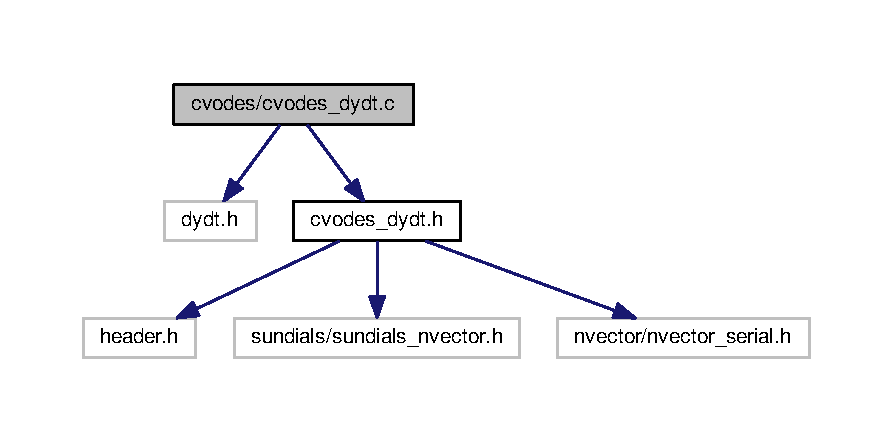
\includegraphics[width=350pt]{cvodes__dydt_8c__incl}
\end{center}
\end{figure}
\subsection*{Functions}
\begin{DoxyCompactItemize}
\item 
int \hyperlink{cvodes__dydt_8c_a82cd83daa4f10afee055813435c6f5b1}{dydt\+\_\+cvodes} (realtype t, N\+\_\+\+Vector y, N\+\_\+\+Vector ydot, void $\ast$f)
\end{DoxyCompactItemize}


\subsection{Detailed Description}
C\+V\+O\+D\+Es Wrapper for the R\+HS function. 



\subsection{Function Documentation}
\index{cvodes\+\_\+dydt.\+c@{cvodes\+\_\+dydt.\+c}!dydt\+\_\+cvodes@{dydt\+\_\+cvodes}}
\index{dydt\+\_\+cvodes@{dydt\+\_\+cvodes}!cvodes\+\_\+dydt.\+c@{cvodes\+\_\+dydt.\+c}}
\subsubsection[{\texorpdfstring{dydt\+\_\+cvodes(realtype t, N\+\_\+\+Vector y, N\+\_\+\+Vector ydot, void $\ast$f)}{dydt_cvodes(realtype t, N_Vector y, N_Vector ydot, void *f)}}]{\setlength{\rightskip}{0pt plus 5cm}int dydt\+\_\+cvodes (
\begin{DoxyParamCaption}
\item[{realtype}]{t, }
\item[{N\+\_\+\+Vector}]{y, }
\item[{N\+\_\+\+Vector}]{ydot, }
\item[{void $\ast$}]{f}
\end{DoxyParamCaption}
)}\hypertarget{cvodes__dydt_8c_a82cd83daa4f10afee055813435c6f5b1}{}\label{cvodes__dydt_8c_a82cd83daa4f10afee055813435c6f5b1}
This method translates the N\+\_\+\+Vector y and ydot\textquotesingle{}s to simple double pointers that may be passed to the internal dydt function. Additionally, the user data (f) is cast to a double as supplied as the \textquotesingle{}Pressure\textquotesingle{} parameter for dydt. 
\hypertarget{cvodes__dydt_8h}{}\section{cvodes/cvodes\+\_\+dydt.h File Reference}
\label{cvodes__dydt_8h}\index{cvodes/cvodes\+\_\+dydt.\+h@{cvodes/cvodes\+\_\+dydt.\+h}}


Header file for C\+V\+O\+D\+Es interface to R\+HS of O\+D\+Es.  


{\ttfamily \#include \char`\"{}header.\+h\char`\"{}}\\*
{\ttfamily \#include \char`\"{}sundials/sundials\+\_\+nvector.\+h\char`\"{}}\\*
{\ttfamily \#include \char`\"{}nvector/nvector\+\_\+serial.\+h\char`\"{}}\\*
Include dependency graph for cvodes\+\_\+dydt.\+h\+:\nopagebreak
\begin{figure}[H]
\begin{center}
\leavevmode
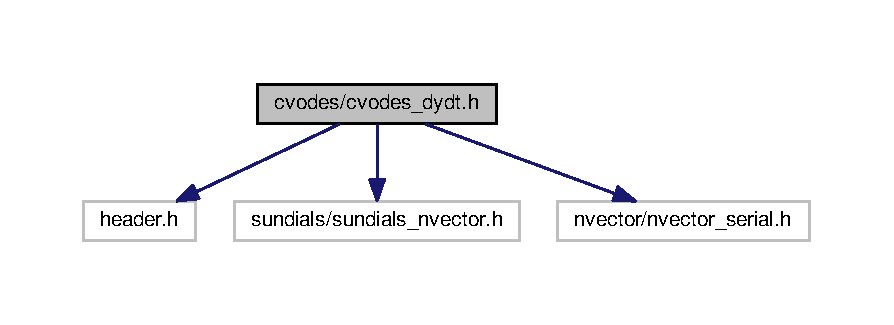
\includegraphics[width=350pt]{cvodes__dydt_8h__incl}
\end{center}
\end{figure}
This graph shows which files directly or indirectly include this file\+:\nopagebreak
\begin{figure}[H]
\begin{center}
\leavevmode
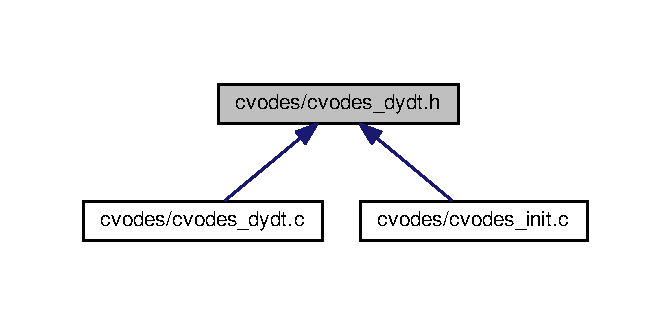
\includegraphics[width=195pt]{cvodes__dydt_8h__dep__incl}
\end{center}
\end{figure}
\subsection*{Functions}
\begin{DoxyCompactItemize}
\item 
int \hyperlink{cvodes__dydt_8h_ae27d76b55607dee9941b4d4e9962e065}{dydt\+\_\+cvodes} (double t, N\+\_\+\+Vector y, N\+\_\+\+Vector ydot, void $\ast$f)
\begin{DoxyCompactList}\small\item\em The C\+V\+O\+D\+Es R\+HS interface. \end{DoxyCompactList}\end{DoxyCompactItemize}


\subsection{Detailed Description}
Header file for C\+V\+O\+D\+Es interface to R\+HS of O\+D\+Es. 

This defines an interface to the right hand side of the O\+D\+Es to pass to C\+V\+O\+D\+Es 

\subsection{Function Documentation}
\index{cvodes\+\_\+dydt.\+h@{cvodes\+\_\+dydt.\+h}!dydt\+\_\+cvodes@{dydt\+\_\+cvodes}}
\index{dydt\+\_\+cvodes@{dydt\+\_\+cvodes}!cvodes\+\_\+dydt.\+h@{cvodes\+\_\+dydt.\+h}}
\subsubsection[{\texorpdfstring{dydt\+\_\+cvodes(double t, N\+\_\+\+Vector y, N\+\_\+\+Vector ydot, void $\ast$f)}{dydt_cvodes(double t, N_Vector y, N_Vector ydot, void *f)}}]{\setlength{\rightskip}{0pt plus 5cm}int dydt\+\_\+cvodes (
\begin{DoxyParamCaption}
\item[{double}]{t, }
\item[{N\+\_\+\+Vector}]{y, }
\item[{N\+\_\+\+Vector}]{ydot, }
\item[{void $\ast$}]{f}
\end{DoxyParamCaption}
)}\hypertarget{cvodes__dydt_8h_ae27d76b55607dee9941b4d4e9962e065}{}\label{cvodes__dydt_8h_ae27d76b55607dee9941b4d4e9962e065}


The C\+V\+O\+D\+Es R\+HS interface. 


\begin{DoxyParams}{Parameters}
{\em t} & The current time of the system \\
\hline
{\em y} & The current state vector (in C\+V\+O\+DE format) \\
\hline
{\em ydot} & The R\+HS vector to be populated (in C\+V\+O\+DE format) \\
\hline
{\em f} & User data set during C\+V\+O\+D\+Es setup (e.\+g. the system pressure) \\
\hline
\end{DoxyParams}
\begin{DoxyReturn}{Returns}
cvode\+\_\+return\+\_\+code The C\+V\+O\+DE output constant returned (see sec B.\+2 of C\+V\+O\+DE documentation), currently always returns C\+V\+\_\+\+S\+U\+C\+C\+E\+SS 
\end{DoxyReturn}

\hypertarget{cvodes__init_8c}{}\section{cvodes/cvodes\+\_\+init.c File Reference}
\label{cvodes__init_8c}\index{cvodes/cvodes\+\_\+init.\+c@{cvodes/cvodes\+\_\+init.\+c}}


Implementation of the necessary initialization for the C\+V\+O\+DE interface.  


{\ttfamily \#include \char`\"{}header.\+h\char`\"{}}\\*
{\ttfamily \#include \char`\"{}solver\+\_\+options.\+h\char`\"{}}\\*
{\ttfamily \#include \char`\"{}cvodes\+\_\+dydt.\+h\char`\"{}}\\*
{\ttfamily \#include \char`\"{}cvodes\+\_\+jac.\+h\char`\"{}}\\*
{\ttfamily \#include \char`\"{}sundials/sundials\+\_\+types.\+h\char`\"{}}\\*
{\ttfamily \#include \char`\"{}sundials/sundials\+\_\+math.\+h\char`\"{}}\\*
{\ttfamily \#include \char`\"{}sundials/sundials\+\_\+nvector.\+h\char`\"{}}\\*
{\ttfamily \#include \char`\"{}nvector/nvector\+\_\+serial.\+h\char`\"{}}\\*
{\ttfamily \#include \char`\"{}cvodes/cvodes.\+h\char`\"{}}\\*
{\ttfamily \#include \char`\"{}cvodes/cvodes\+\_\+lapack.\+h\char`\"{}}\\*
Include dependency graph for cvodes\+\_\+init.\+c\+:\nopagebreak
\begin{figure}[H]
\begin{center}
\leavevmode
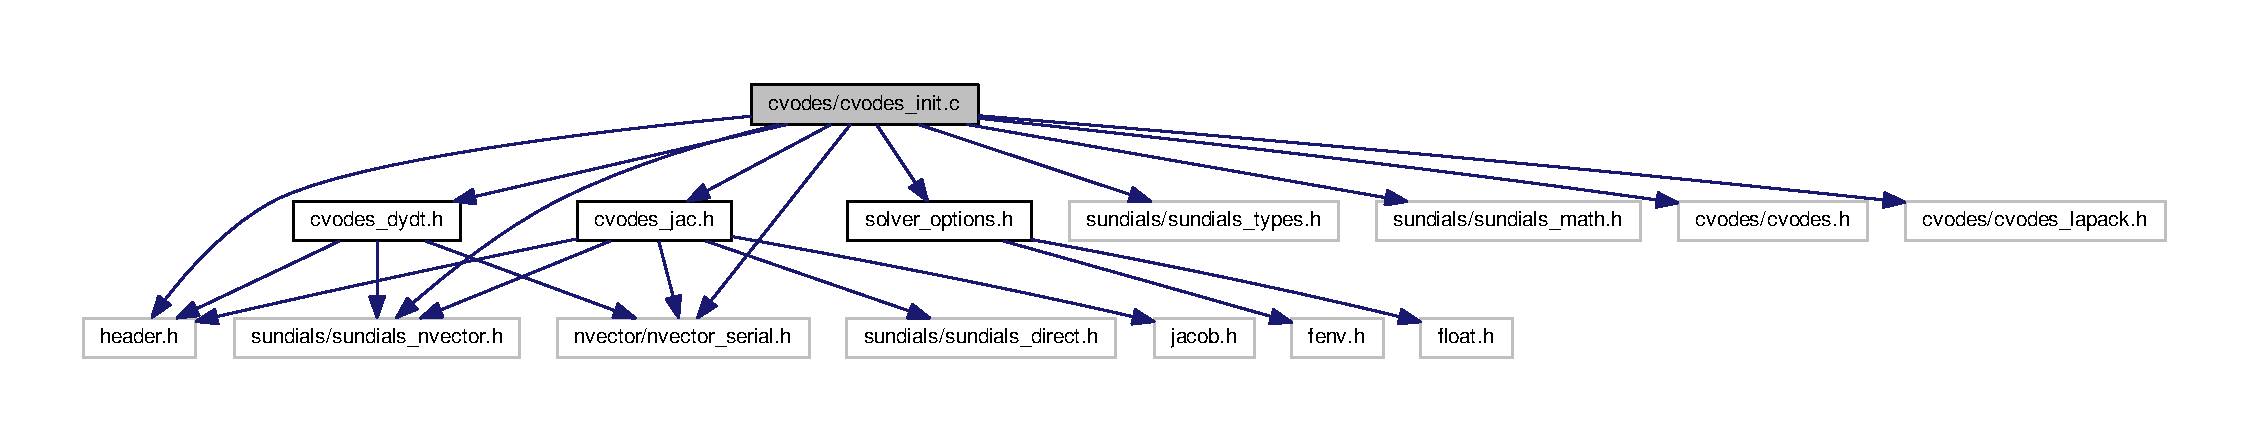
\includegraphics[width=350pt]{cvodes__init_8c__incl}
\end{center}
\end{figure}
\subsection*{Namespaces}
\begin{DoxyCompactItemize}
\item 
 \hyperlink{namespacecvode}{cvode}
\end{DoxyCompactItemize}
\subsection*{Functions}
\begin{DoxyCompactItemize}
\item 
int \hyperlink{namespacecvode_aa10a063b2a82d5b49c2bb338f16ddae4}{cvode\+::dydt\+\_\+cvodes} (double t, N\+\_\+\+Vector y, N\+\_\+\+Vector ydot, void $\ast$f)
\begin{DoxyCompactList}\small\item\em The C\+V\+O\+D\+Es R\+HS interface. \end{DoxyCompactList}\item 
int \hyperlink{namespacecvode_ab2efc395730d25bedc496a62e7896d24}{cvode\+::eval\+\_\+jacob\+\_\+cvodes} (long int N, double t, N\+\_\+\+Vector y, N\+\_\+\+Vector ydot, Dls\+Mat Jac, void $\ast$f, N\+\_\+\+Vector tmp1, N\+\_\+\+Vector tmp2, N\+\_\+\+Vector tmp3)
\begin{DoxyCompactList}\small\item\em The C\+V\+O\+D\+Es Jacobian interface for a direct dense Jacobian. \end{DoxyCompactList}\item 
void \hyperlink{namespacecvode_abe146525cea80d8032cd30b4441b5872}{cvode\+::initialize\+\_\+solver} (int num\+\_\+threads)
\begin{DoxyCompactList}\small\item\em Creates/\+Checks the C\+V\+O\+DE solvers for the specified number of threads. \end{DoxyCompactList}\item 
void \hyperlink{namespacecvode_ac9bc4957bff6721dae9d7e4cc470d184}{cvode\+::cleanup\+\_\+solver} (int num\+\_\+threads)
\begin{DoxyCompactList}\small\item\em Cleans up the created C\+V\+O\+DE solvers. \end{DoxyCompactList}\item 
const char $\ast$ \hyperlink{namespacecvode_a3a26024b8dc2ce6f8b2afcfb7c82c79f}{cvode\+::solver\+\_\+name} ()
\begin{DoxyCompactList}\small\item\em Returns the C\+V\+O\+DE solver name. \end{DoxyCompactList}\item 
void \hyperlink{namespacecvode_a9113d5fb0e19fa927d73b64c397ecd09}{cvode\+::init\+\_\+solver\+\_\+log} ()
\item 
void \hyperlink{namespacecvode_af7eb796b6829fecab506fb6dfec39be0}{cvode\+::solver\+\_\+log} ()
\end{DoxyCompactItemize}
\subsection*{Variables}
\begin{DoxyCompactItemize}
\item 
N\+\_\+\+Vector $\ast$ \hyperlink{namespacecvode_a84c47b6a9f2bedf2c5c80429079fc8e3}{cvode\+::y\+\_\+locals}
\item 
double $\ast$ \hyperlink{namespacecvode_adae183039534044ead74e1c1a786a36c}{cvode\+::y\+\_\+local\+\_\+vectors}
\item 
void $\ast$$\ast$ \hyperlink{namespacecvode_a9290e27651628dff03f82f42eafd3079}{cvode\+::integrators}
\end{DoxyCompactItemize}


\subsection{Detailed Description}
Implementation of the necessary initialization for the C\+V\+O\+DE interface. 

\begin{DoxyAuthor}{Author}
Nicholas Curtis 
\end{DoxyAuthor}
\begin{DoxyDate}{Date}
03/09/2015 
\end{DoxyDate}

\hypertarget{cvodes__jac_8c}{}\section{cvodes/cvodes\+\_\+jac.c File Reference}
\label{cvodes__jac_8c}\index{cvodes/cvodes\+\_\+jac.\+c@{cvodes/cvodes\+\_\+jac.\+c}}


A simple wrapper, allowing for use of the analytical jacobian w/ C\+V\+O\+D\+ES.  


{\ttfamily \#include \char`\"{}cvodes\+\_\+jac.\+h\char`\"{}}\\*
Include dependency graph for cvodes\+\_\+jac.\+c\+:\nopagebreak
\begin{figure}[H]
\begin{center}
\leavevmode
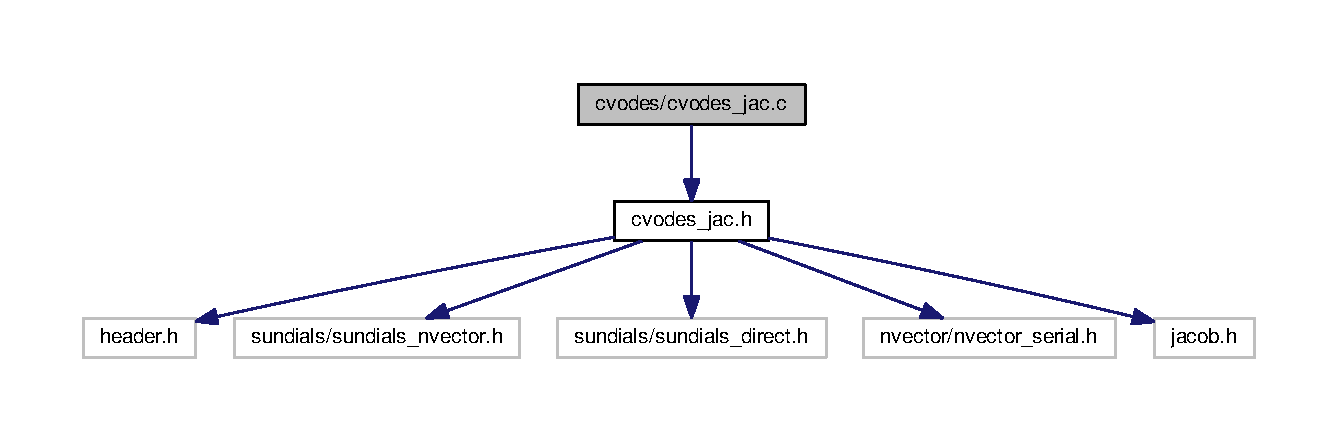
\includegraphics[width=350pt]{cvodes__jac_8c__incl}
\end{center}
\end{figure}
\subsection*{Functions}
\begin{DoxyCompactItemize}
\item 
int \hyperlink{cvodes__jac_8c_a25a1370ef7b8492e115d1ff20863d318}{eval\+\_\+jacob\+\_\+cvodes} (long int N, double t, N\+\_\+\+Vector y, N\+\_\+\+Vector ydot, Dls\+Mat jac, void $\ast$f, N\+\_\+\+Vector tmp1, N\+\_\+\+Vector tmp2, N\+\_\+\+Vector tmp3)
\begin{DoxyCompactList}\small\item\em The C\+V\+O\+D\+Es Jacobian interface for a direct dense Jacobian. \end{DoxyCompactList}\end{DoxyCompactItemize}


\subsection{Detailed Description}
A simple wrapper, allowing for use of the analytical jacobian w/ C\+V\+O\+D\+ES. 



\subsection{Function Documentation}
\index{cvodes\+\_\+jac.\+c@{cvodes\+\_\+jac.\+c}!eval\+\_\+jacob\+\_\+cvodes@{eval\+\_\+jacob\+\_\+cvodes}}
\index{eval\+\_\+jacob\+\_\+cvodes@{eval\+\_\+jacob\+\_\+cvodes}!cvodes\+\_\+jac.\+c@{cvodes\+\_\+jac.\+c}}
\subsubsection[{\texorpdfstring{eval\+\_\+jacob\+\_\+cvodes(long int N, double t, N\+\_\+\+Vector y, N\+\_\+\+Vector ydot, Dls\+Mat jac, void $\ast$f, N\+\_\+\+Vector tmp1, N\+\_\+\+Vector tmp2, N\+\_\+\+Vector tmp3)}{eval_jacob_cvodes(long int N, double t, N_Vector y, N_Vector ydot, DlsMat jac, void *f, N_Vector tmp1, N_Vector tmp2, N_Vector tmp3)}}]{\setlength{\rightskip}{0pt plus 5cm}int eval\+\_\+jacob\+\_\+cvodes (
\begin{DoxyParamCaption}
\item[{long int}]{N, }
\item[{double}]{t, }
\item[{N\+\_\+\+Vector}]{y, }
\item[{N\+\_\+\+Vector}]{ydot, }
\item[{Dls\+Mat}]{jac, }
\item[{void $\ast$}]{f, }
\item[{N\+\_\+\+Vector}]{tmp1, }
\item[{N\+\_\+\+Vector}]{tmp2, }
\item[{N\+\_\+\+Vector}]{tmp3}
\end{DoxyParamCaption}
)}\hypertarget{cvodes__jac_8c_a25a1370ef7b8492e115d1ff20863d318}{}\label{cvodes__jac_8c_a25a1370ef7b8492e115d1ff20863d318}


The C\+V\+O\+D\+Es Jacobian interface for a direct dense Jacobian. 

This function converts the N\+\_\+\+Vectors {\ttfamily y} and {\ttfamily y\+\_\+dot} to simple double pointers, the user data {\ttfamily f} to a double and outputs the Jacobian supplied by {\ttfamily eval\+\_\+jacob} to the C\+V\+O\+DE jacobian {\ttfamily jac} Currently, C\+V\+\_\+\+S\+U\+C\+C\+E\+SS is always returned. 
\hypertarget{cvodes__jac_8h}{}\section{cvodes/cvodes\+\_\+jac.h File Reference}
\label{cvodes__jac_8h}\index{cvodes/cvodes\+\_\+jac.\+h@{cvodes/cvodes\+\_\+jac.\+h}}


A simple wrapper, allowing for use of the analytical jacobian w/ C\+V\+O\+D\+ES.  


{\ttfamily \#include \char`\"{}header.\+h\char`\"{}}\\*
{\ttfamily \#include \char`\"{}sundials/sundials\+\_\+nvector.\+h\char`\"{}}\\*
{\ttfamily \#include \char`\"{}sundials/sundials\+\_\+direct.\+h\char`\"{}}\\*
{\ttfamily \#include \char`\"{}nvector/nvector\+\_\+serial.\+h\char`\"{}}\\*
{\ttfamily \#include \char`\"{}jacob.\+h\char`\"{}}\\*
Include dependency graph for cvodes\+\_\+jac.\+h\+:\nopagebreak
\begin{figure}[H]
\begin{center}
\leavevmode
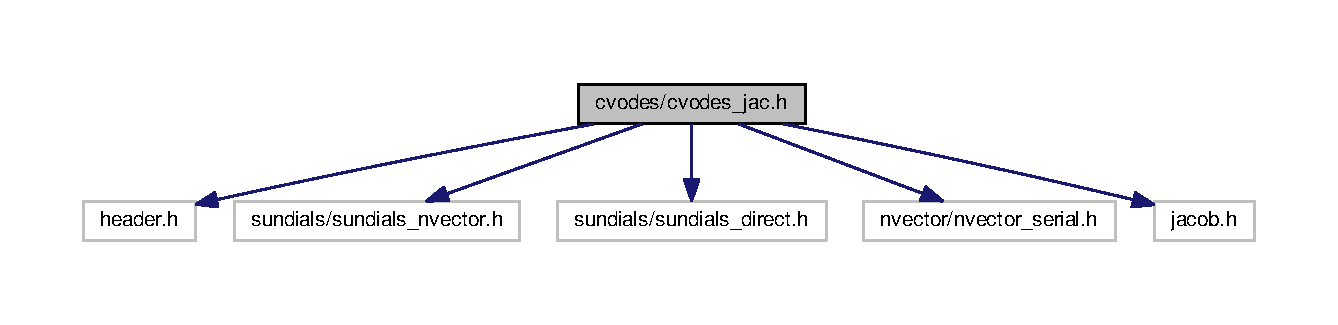
\includegraphics[width=350pt]{cvodes__jac_8h__incl}
\end{center}
\end{figure}
This graph shows which files directly or indirectly include this file\+:\nopagebreak
\begin{figure}[H]
\begin{center}
\leavevmode
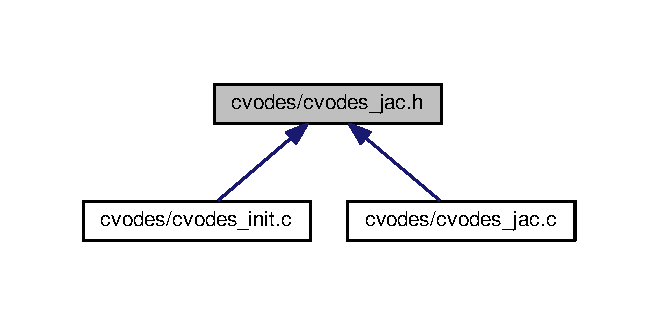
\includegraphics[width=316pt]{cvodes__jac_8h__dep__incl}
\end{center}
\end{figure}
\subsection*{Macros}
\begin{DoxyCompactItemize}
\item 
\#define \hyperlink{cvodes__init_8c_afc974a5ba6f507ebbdeb4dd3f8c5abdc}{J\+A\+C\+\_\+\+H\+E\+A\+D\+\_\+\+C\+V\+O\+D\+ES}
\end{DoxyCompactItemize}
\subsection*{Functions}
\begin{DoxyCompactItemize}
\item 
int \hyperlink{cvodes__jac_8h_ace0ee8931b5755b80309735167af0b86}{eval\+\_\+jacob\+\_\+cvodes} (long int N, double t, N\+\_\+\+Vector y, N\+\_\+\+Vector ydot, Dls\+Mat Jac, void $\ast$f, N\+\_\+\+Vector tmp1, N\+\_\+\+Vector tmp2, N\+\_\+\+Vector tmp3)
\begin{DoxyCompactList}\small\item\em The C\+V\+O\+D\+Es Jacobian interface for a direct dense Jacobian. \end{DoxyCompactList}\end{DoxyCompactItemize}


\subsection{Detailed Description}
A simple wrapper, allowing for use of the analytical jacobian w/ C\+V\+O\+D\+ES. 



\subsection{Macro Definition Documentation}
\index{cvodes\+\_\+jac.\+h@{cvodes\+\_\+jac.\+h}!J\+A\+C\+\_\+\+H\+E\+A\+D\+\_\+\+C\+V\+O\+D\+ES@{J\+A\+C\+\_\+\+H\+E\+A\+D\+\_\+\+C\+V\+O\+D\+ES}}
\index{J\+A\+C\+\_\+\+H\+E\+A\+D\+\_\+\+C\+V\+O\+D\+ES@{J\+A\+C\+\_\+\+H\+E\+A\+D\+\_\+\+C\+V\+O\+D\+ES}!cvodes\+\_\+jac.\+h@{cvodes\+\_\+jac.\+h}}
\subsubsection[{\texorpdfstring{J\+A\+C\+\_\+\+H\+E\+A\+D\+\_\+\+C\+V\+O\+D\+ES}{JAC_HEAD_CVODES}}]{\setlength{\rightskip}{0pt plus 5cm}\#define J\+A\+C\+\_\+\+H\+E\+A\+D\+\_\+\+C\+V\+O\+D\+ES}\hypertarget{cvodes__init_8c_afc974a5ba6f507ebbdeb4dd3f8c5abdc}{}\label{cvodes__init_8c_afc974a5ba6f507ebbdeb4dd3f8c5abdc}


\subsection{Function Documentation}
\index{cvodes\+\_\+jac.\+h@{cvodes\+\_\+jac.\+h}!eval\+\_\+jacob\+\_\+cvodes@{eval\+\_\+jacob\+\_\+cvodes}}
\index{eval\+\_\+jacob\+\_\+cvodes@{eval\+\_\+jacob\+\_\+cvodes}!cvodes\+\_\+jac.\+h@{cvodes\+\_\+jac.\+h}}
\subsubsection[{\texorpdfstring{eval\+\_\+jacob\+\_\+cvodes(long int N, double t, N\+\_\+\+Vector y, N\+\_\+\+Vector ydot, Dls\+Mat Jac, void $\ast$f, N\+\_\+\+Vector tmp1, N\+\_\+\+Vector tmp2, N\+\_\+\+Vector tmp3)}{eval_jacob_cvodes(long int N, double t, N_Vector y, N_Vector ydot, DlsMat Jac, void *f, N_Vector tmp1, N_Vector tmp2, N_Vector tmp3)}}]{\setlength{\rightskip}{0pt plus 5cm}int eval\+\_\+jacob\+\_\+cvodes (
\begin{DoxyParamCaption}
\item[{long int}]{N, }
\item[{double}]{t, }
\item[{N\+\_\+\+Vector}]{y, }
\item[{N\+\_\+\+Vector}]{ydot, }
\item[{Dls\+Mat}]{jac, }
\item[{void $\ast$}]{f, }
\item[{N\+\_\+\+Vector}]{tmp1, }
\item[{N\+\_\+\+Vector}]{tmp2, }
\item[{N\+\_\+\+Vector}]{tmp3}
\end{DoxyParamCaption}
)}\hypertarget{cvodes__jac_8h_ace0ee8931b5755b80309735167af0b86}{}\label{cvodes__jac_8h_ace0ee8931b5755b80309735167af0b86}


The C\+V\+O\+D\+Es Jacobian interface for a direct dense Jacobian. 


\begin{DoxyParams}{Parameters}
{\em N} & the problem size \\
\hline
{\em t} & The current time of the system \\
\hline
{\em y} & The current state vector (in C\+V\+O\+DE format) \\
\hline
{\em ydot} & The R\+HS vector to be populated (in C\+V\+O\+DE format) \\
\hline
{\em jac} & The Jacobian matrix (in C\+V\+O\+DE format) to output to \\
\hline
{\em f} & User data set during C\+V\+O\+D\+Es setup (e.\+g. the system pressure) \\
\hline
{\em tmp1} & Temporary storage used by C\+V\+O\+D\+Es \\
\hline
{\em tmp2} & Temporary storage used by C\+V\+O\+D\+Es \\
\hline
{\em tmp3} & Temporary storage used by C\+V\+O\+D\+Es \\
\hline
\end{DoxyParams}
\begin{DoxyReturn}{Returns}
cvode\+\_\+return\+\_\+code The C\+V\+O\+DE output constant returned (see sec B.\+2 of C\+V\+O\+DE documentation), currently always returns C\+V\+\_\+\+S\+U\+C\+C\+E\+SS
\end{DoxyReturn}
This function converts the N\+\_\+\+Vectors {\ttfamily y} and {\ttfamily y\+\_\+dot} to simple double pointers, the user data {\ttfamily f} to a double and outputs the Jacobian supplied by {\ttfamily eval\+\_\+jacob} to the C\+V\+O\+DE jacobian {\ttfamily jac} Currently, C\+V\+\_\+\+S\+U\+C\+C\+E\+SS is always returned. 
\hypertarget{solver__cvodes_8c}{}\section{cvodes/solver\+\_\+cvodes.c File Reference}
\label{solver__cvodes_8c}\index{cvodes/solver\+\_\+cvodes.\+c@{cvodes/solver\+\_\+cvodes.\+c}}
{\ttfamily \#include \char`\"{}header.\+h\char`\"{}}\\*
{\ttfamily \#include \char`\"{}solver.\+h\char`\"{}}\\*
{\ttfamily \#include \char`\"{}sundials/sundials\+\_\+types.\+h\char`\"{}}\\*
{\ttfamily \#include \char`\"{}sundials/sundials\+\_\+math.\+h\char`\"{}}\\*
{\ttfamily \#include \char`\"{}sundials/sundials\+\_\+nvector.\+h\char`\"{}}\\*
{\ttfamily \#include \char`\"{}nvector/nvector\+\_\+serial.\+h\char`\"{}}\\*
{\ttfamily \#include \char`\"{}cvodes/cvodes.\+h\char`\"{}}\\*
{\ttfamily \#include \char`\"{}cvodes/cvodes\+\_\+lapack.\+h\char`\"{}}\\*
Include dependency graph for solver\+\_\+cvodes.\+c\+:\nopagebreak
\begin{figure}[H]
\begin{center}
\leavevmode
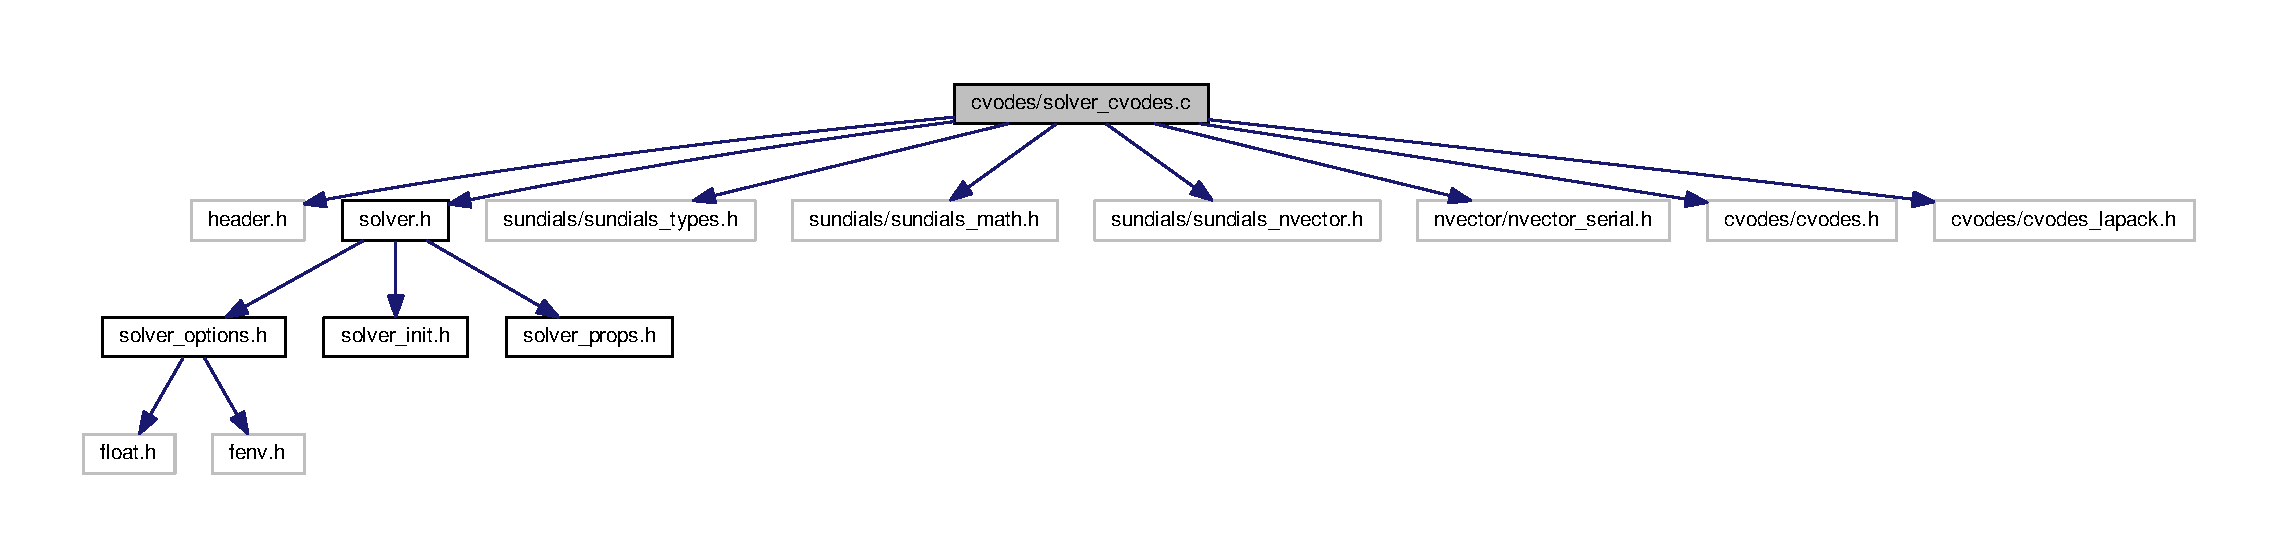
\includegraphics[width=350pt]{solver__cvodes_8c__incl}
\end{center}
\end{figure}
\subsection*{Functions}
\begin{DoxyCompactItemize}
\item 
void \hyperlink{solver__cvodes_8c_a68bf42894bc3d748ef9d7e54e4ba4d30}{int\+Driver} (const int N\+UM, const double t, const double t\+\_\+end, const double $\ast$pr\+\_\+global, double $\ast$y\+\_\+global)
\end{DoxyCompactItemize}
\subsection*{Variables}
\begin{DoxyCompactItemize}
\item 
N\+\_\+\+Vector $\ast$ \hyperlink{solver__cvodes_8c_a879c5a17d799c66d4f4c57695a1a4a9f}{y\+\_\+locals}
\item 
double $\ast$ \hyperlink{solver__cvodes_8c_af6c0090b9c0312d8ea355108bca0fd06}{y\+\_\+local\+\_\+vectors}
\item 
void $\ast$$\ast$ \hyperlink{solver__cvodes_8c_a37bbe31792d35bffd1b6d28e1c6cee1b}{integrators}
\end{DoxyCompactItemize}


\subsection{Function Documentation}
\index{solver\+\_\+cvodes.\+c@{solver\+\_\+cvodes.\+c}!int\+Driver@{int\+Driver}}
\index{int\+Driver@{int\+Driver}!solver\+\_\+cvodes.\+c@{solver\+\_\+cvodes.\+c}}
\subsubsection[{\texorpdfstring{int\+Driver(const int N\+U\+M, const double t, const double t\+\_\+end, const double $\ast$pr\+\_\+global, double $\ast$y\+\_\+global)}{intDriver(const int NUM, const double t, const double t_end, const double *pr_global, double *y_global)}}]{\setlength{\rightskip}{0pt plus 5cm}void int\+Driver (
\begin{DoxyParamCaption}
\item[{const int}]{N\+UM, }
\item[{const double}]{t, }
\item[{const double}]{t\+\_\+end, }
\item[{const double $\ast$}]{pr\+\_\+global, }
\item[{double $\ast$}]{y\+\_\+global}
\end{DoxyParamCaption}
)}\hypertarget{solver__cvodes_8c_a68bf42894bc3d748ef9d7e54e4ba4d30}{}\label{solver__cvodes_8c_a68bf42894bc3d748ef9d7e54e4ba4d30}


\subsection{Variable Documentation}
\index{solver\+\_\+cvodes.\+c@{solver\+\_\+cvodes.\+c}!integrators@{integrators}}
\index{integrators@{integrators}!solver\+\_\+cvodes.\+c@{solver\+\_\+cvodes.\+c}}
\subsubsection[{\texorpdfstring{integrators}{integrators}}]{\setlength{\rightskip}{0pt plus 5cm}void$\ast$$\ast$ integrators}\hypertarget{solver__cvodes_8c_a37bbe31792d35bffd1b6d28e1c6cee1b}{}\label{solver__cvodes_8c_a37bbe31792d35bffd1b6d28e1c6cee1b}
The stored C\+V\+O\+DE integrator objects \index{solver\+\_\+cvodes.\+c@{solver\+\_\+cvodes.\+c}!y\+\_\+local\+\_\+vectors@{y\+\_\+local\+\_\+vectors}}
\index{y\+\_\+local\+\_\+vectors@{y\+\_\+local\+\_\+vectors}!solver\+\_\+cvodes.\+c@{solver\+\_\+cvodes.\+c}}
\subsubsection[{\texorpdfstring{y\+\_\+local\+\_\+vectors}{y_local_vectors}}]{\setlength{\rightskip}{0pt plus 5cm}double$\ast$ y\+\_\+local\+\_\+vectors}\hypertarget{solver__cvodes_8c_af6c0090b9c0312d8ea355108bca0fd06}{}\label{solver__cvodes_8c_af6c0090b9c0312d8ea355108bca0fd06}
The base state vectors used in N\+\_\+\+Vector creation \index{solver\+\_\+cvodes.\+c@{solver\+\_\+cvodes.\+c}!y\+\_\+locals@{y\+\_\+locals}}
\index{y\+\_\+locals@{y\+\_\+locals}!solver\+\_\+cvodes.\+c@{solver\+\_\+cvodes.\+c}}
\subsubsection[{\texorpdfstring{y\+\_\+locals}{y_locals}}]{\setlength{\rightskip}{0pt plus 5cm}N\+\_\+\+Vector$\ast$ y\+\_\+locals}\hypertarget{solver__cvodes_8c_a879c5a17d799c66d4f4c57695a1a4a9f}{}\label{solver__cvodes_8c_a879c5a17d799c66d4f4c57695a1a4a9f}
The state vectors used in C\+V\+O\+DE operation 
\hypertarget{arnoldi_8cuh}{}\section{exponential\+\_\+integrators/arnoldi.cuh File Reference}
\label{arnoldi_8cuh}\index{exponential\+\_\+integrators/arnoldi.\+cuh@{exponential\+\_\+integrators/arnoldi.\+cuh}}
{\ttfamily \#include $<$string.\+h$>$}\\*
{\ttfamily \#include \char`\"{}header.\+cuh\char`\"{}}\\*
{\ttfamily \#include \char`\"{}phi\+A\+Hessenberg.\+cuh\char`\"{}}\\*
{\ttfamily \#include \char`\"{}exponential\+\_\+linear\+\_\+algebra.\+cuh\char`\"{}}\\*
Include dependency graph for arnoldi.\+cuh\+:\nopagebreak
\begin{figure}[H]
\begin{center}
\leavevmode
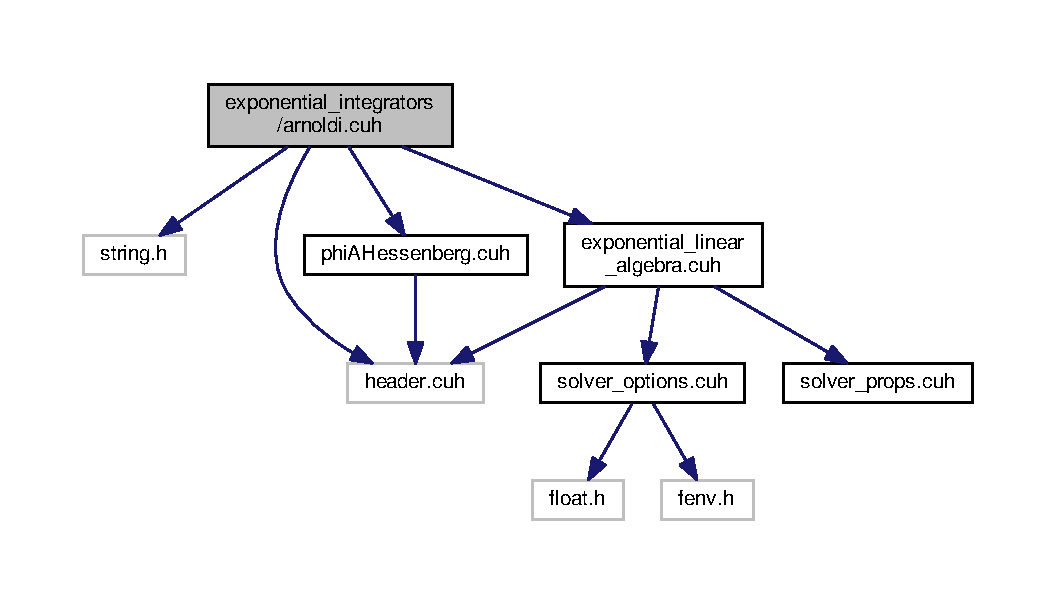
\includegraphics[width=350pt]{arnoldi_8cuh__incl}
\end{center}
\end{figure}
This graph shows which files directly or indirectly include this file\+:\nopagebreak
\begin{figure}[H]
\begin{center}
\leavevmode
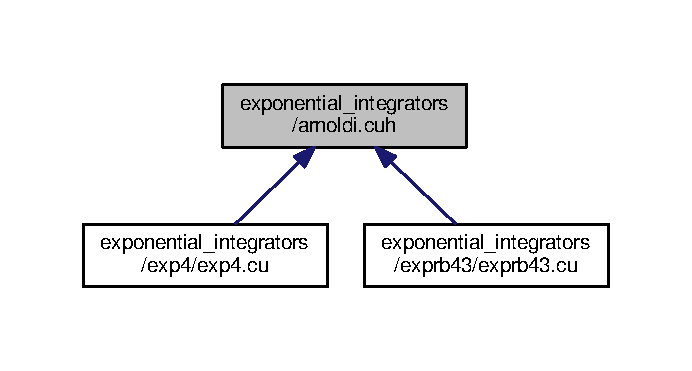
\includegraphics[width=332pt]{arnoldi_8cuh__dep__incl}
\end{center}
\end{figure}
\subsection*{Macros}
\begin{DoxyCompactItemize}
\item 
\#define \hyperlink{arnoldi_8cuh_abeda2f8ea38aa8f4d7bd240e22181d1c}{A\+R\+N\+O\+L\+D\+I\+\_\+\+C\+UH}
\end{DoxyCompactItemize}
\subsection*{Functions}
\begin{DoxyCompactItemize}
\item 
\+\_\+\+\_\+device\+\_\+\+\_\+ int \hyperlink{arnoldi_8cuh_ab3811b1c15ea17c96f86d55e137e4374}{arnoldi} (const double \hyperlink{inverse_8cu_adbb4f3f3af5f968a94f717729803c88d}{scale}, const int p, const double h, const double $\ast$\+\_\+\+\_\+restrict\+\_\+\+\_\+ A, const \hyperlink{structsolver__memory}{solver\+\_\+memory} $\ast$\+\_\+\+\_\+restrict\+\_\+\+\_\+ solver, const double $\ast$\+\_\+\+\_\+restrict\+\_\+\+\_\+ v, double $\ast$\+\_\+\+\_\+restrict\+\_\+\+\_\+ beta, double $\ast$\+\_\+\+\_\+restrict\+\_\+\+\_\+ work, cu\+Double\+Complex $\ast$\+\_\+\+\_\+restrict\+\_\+\+\_\+ work2)
\begin{DoxyCompactList}\small\item\em Runs the arnoldi iteration to calculate the Krylov projection. \end{DoxyCompactList}\end{DoxyCompactItemize}
\subsection*{Variables}
\begin{DoxyCompactItemize}
\item 
\+\_\+\+\_\+constant\+\_\+\+\_\+ int \hyperlink{arnoldi_8cuh_a3e638b2302ac9e7f341e07f7eb51ec5d}{index\+\_\+list} \mbox{[}23\mbox{]} = \{1, 2, 3, 4, 5, 6, 7, 9, 11, 14, 17, 21, 27, 34, 42, 53, 67, 84, 106, 133, 167, 211, 265\}
\begin{DoxyCompactList}\small\item\em The list of indicies to check the Krylov projection error at. \end{DoxyCompactList}\end{DoxyCompactItemize}


\subsection{Macro Definition Documentation}
\index{arnoldi.\+cuh@{arnoldi.\+cuh}!A\+R\+N\+O\+L\+D\+I\+\_\+\+C\+UH@{A\+R\+N\+O\+L\+D\+I\+\_\+\+C\+UH}}
\index{A\+R\+N\+O\+L\+D\+I\+\_\+\+C\+UH@{A\+R\+N\+O\+L\+D\+I\+\_\+\+C\+UH}!arnoldi.\+cuh@{arnoldi.\+cuh}}
\subsubsection[{\texorpdfstring{A\+R\+N\+O\+L\+D\+I\+\_\+\+C\+UH}{ARNOLDI_CUH}}]{\setlength{\rightskip}{0pt plus 5cm}\#define A\+R\+N\+O\+L\+D\+I\+\_\+\+C\+UH}\hypertarget{arnoldi_8cuh_abeda2f8ea38aa8f4d7bd240e22181d1c}{}\label{arnoldi_8cuh_abeda2f8ea38aa8f4d7bd240e22181d1c}


\subsection{Function Documentation}
\index{arnoldi.\+cuh@{arnoldi.\+cuh}!arnoldi@{arnoldi}}
\index{arnoldi@{arnoldi}!arnoldi.\+cuh@{arnoldi.\+cuh}}
\subsubsection[{\texorpdfstring{arnoldi(const double scale, const int p, const double h, const double $\ast$\+\_\+\+\_\+restrict\+\_\+\+\_\+ A, const solver\+\_\+memory $\ast$\+\_\+\+\_\+restrict\+\_\+\+\_\+ solver, const double $\ast$\+\_\+\+\_\+restrict\+\_\+\+\_\+ v, double $\ast$\+\_\+\+\_\+restrict\+\_\+\+\_\+ beta, double $\ast$\+\_\+\+\_\+restrict\+\_\+\+\_\+ work, cu\+Double\+Complex $\ast$\+\_\+\+\_\+restrict\+\_\+\+\_\+ work2)}{arnoldi(const double scale, const int p, const double h, const double *__restrict__ A, const solver_memory *__restrict__ solver, const double *__restrict__ v, double *__restrict__ beta, double *__restrict__ work, cuDoubleComplex *__restrict__ work2)}}]{\setlength{\rightskip}{0pt plus 5cm}int arnoldi (
\begin{DoxyParamCaption}
\item[{const double}]{scale, }
\item[{const int}]{p, }
\item[{const double}]{h, }
\item[{const double $\ast$\+\_\+\+\_\+restrict\+\_\+\+\_\+}]{A, }
\item[{const {\bf solver\+\_\+memory} $\ast$\+\_\+\+\_\+restrict\+\_\+\+\_\+}]{solver, }
\item[{const double $\ast$\+\_\+\+\_\+restrict\+\_\+\+\_\+}]{v, }
\item[{double $\ast$\+\_\+\+\_\+restrict\+\_\+\+\_\+}]{beta, }
\item[{double $\ast$\+\_\+\+\_\+restrict\+\_\+\+\_\+}]{work, }
\item[{cu\+Double\+Complex $\ast$\+\_\+\+\_\+restrict\+\_\+\+\_\+}]{work2}
\end{DoxyParamCaption}
)}\hypertarget{arnoldi_8cuh_ab3811b1c15ea17c96f86d55e137e4374}{}\label{arnoldi_8cuh_ab3811b1c15ea17c96f86d55e137e4374}


Runs the arnoldi iteration to calculate the Krylov projection. 

\begin{DoxyReturn}{Returns}
m -\/ the ending size of the matrix 
\end{DoxyReturn}

\begin{DoxyParams}[1]{Parameters}
\mbox{\tt in}  & {\em scale} & the value to scale the timestep by \\
\hline
\mbox{\tt in}  & {\em p} & the order of the maximum phi function needed \\
\hline
\mbox{\tt in}  & {\em h} & the timestep \\
\hline
\mbox{\tt in}  & {\em A} & the jacobian matrix \\
\hline
\mbox{\tt in,out}  & {\em solver} & the solver memory struct \\
\hline
\mbox{\tt in}  & {\em v} & the vector to use for the krylov subspace \\
\hline
\mbox{\tt out}  & {\em beta} & the norm of the v vector \\
\hline
\mbox{\tt in,out}  & {\em work} & A work vector \\
\hline
\mbox{\tt in,out}  & {\em work2} & A complex work vector \\
\hline
\end{DoxyParams}


\subsection{Variable Documentation}
\index{arnoldi.\+cuh@{arnoldi.\+cuh}!index\+\_\+list@{index\+\_\+list}}
\index{index\+\_\+list@{index\+\_\+list}!arnoldi.\+cuh@{arnoldi.\+cuh}}
\subsubsection[{\texorpdfstring{index\+\_\+list}{index_list}}]{\setlength{\rightskip}{0pt plus 5cm}\+\_\+\+\_\+constant\+\_\+\+\_\+ int index\+\_\+list\mbox{[}23\mbox{]} = \{1, 2, 3, 4, 5, 6, 7, 9, 11, 14, 17, 21, 27, 34, 42, 53, 67, 84, 106, 133, 167, 211, 265\}}\hypertarget{arnoldi_8cuh_a3e638b2302ac9e7f341e07f7eb51ec5d}{}\label{arnoldi_8cuh_a3e638b2302ac9e7f341e07f7eb51ec5d}


The list of indicies to check the Krylov projection error at. 


\hypertarget{arnoldi_8h}{}\section{/home/nick/\+Dropbox/acceler\+Int/exponential\+\_\+integrators/arnoldi.h File Reference}
\label{arnoldi_8h}\index{/home/nick/\+Dropbox/acceler\+Int/exponential\+\_\+integrators/arnoldi.\+h@{/home/nick/\+Dropbox/acceler\+Int/exponential\+\_\+integrators/arnoldi.\+h}}


Implementation of the G\+PU arnoldi iteration methods.  


{\ttfamily \#include $<$string.\+h$>$}\\*
{\ttfamily \#include \char`\"{}header.\+h\char`\"{}}\\*
{\ttfamily \#include \char`\"{}phi\+A\+Hessenberg.\+h\char`\"{}}\\*
{\ttfamily \#include \char`\"{}exponential\+\_\+linear\+\_\+algebra.\+h\char`\"{}}\\*
Include dependency graph for arnoldi.\+h\+:
\nopagebreak
\begin{figure}[H]
\begin{center}
\leavevmode
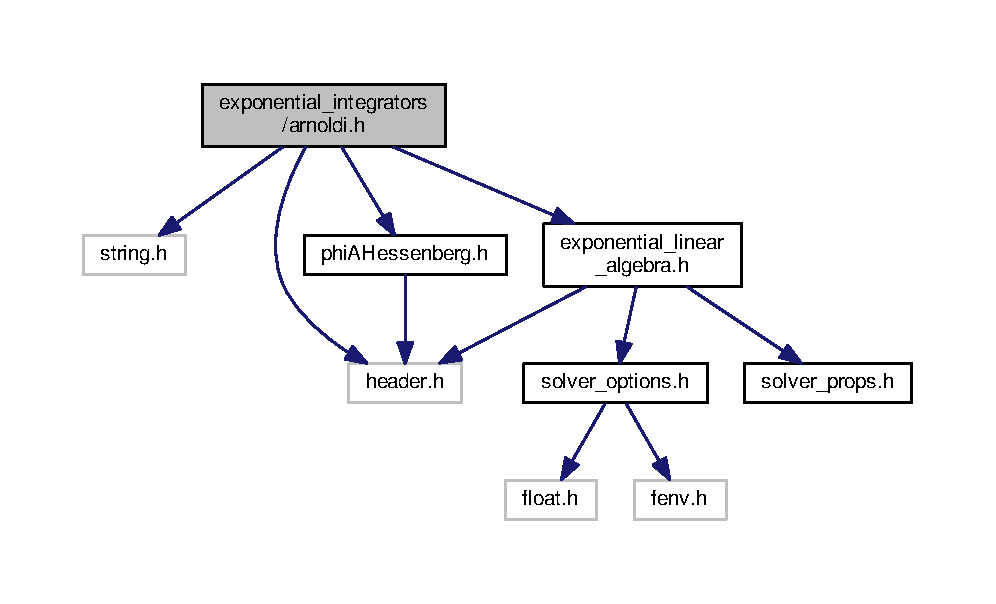
\includegraphics[width=350pt]{arnoldi_8h__incl}
\end{center}
\end{figure}
This graph shows which files directly or indirectly include this file\+:
\nopagebreak
\begin{figure}[H]
\begin{center}
\leavevmode
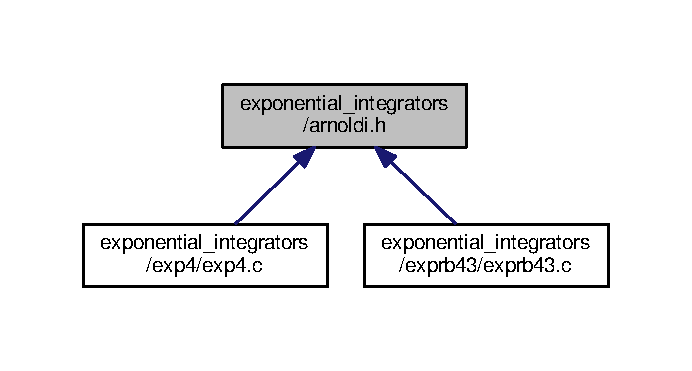
\includegraphics[width=350pt]{arnoldi_8h__dep__incl}
\end{center}
\end{figure}
\subsection*{Functions}
\begin{DoxyCompactItemize}
\item 
static int \hyperlink{arnoldi_8h_a8b64f0d02450612b167702a2ff72fd90}{arnoldi} (const double \hyperlink{inverse_8cu_adbb4f3f3af5f968a94f717729803c88d}{scale}, const int p, const double h, const double $\ast$A, const double $\ast$v, const double $\ast$sc, double $\ast$beta, double $\ast$Vm, double $\ast$Hm, double $\ast$phi\+Hm)
\begin{DoxyCompactList}\small\item\em Runs the arnoldi iteration to calculate the Krylov projection. \end{DoxyCompactList}\end{DoxyCompactItemize}
\subsection*{Variables}
\begin{DoxyCompactItemize}
\item 
static int \hyperlink{arnoldi_8h_ac4b10b70a18d8ce035332064894b9b99}{index\+\_\+list} \mbox{[}23\mbox{]} = \{1, 2, 3, 4, 5, 6, 7, 9, 11, 14, 17, 21, 27, 34, 42, 53, 67, 84, 106, 133, 167, 211, 265\}
\begin{DoxyCompactList}\small\item\em The list of indicies to check the Krylov projection error at. \end{DoxyCompactList}\end{DoxyCompactItemize}


\subsection{Detailed Description}
Implementation of the G\+PU arnoldi iteration methods. 

Implementation of the arnoldi iteration methods.

\begin{DoxyAuthor}{Author}
Nicholas Curtis 
\end{DoxyAuthor}
\begin{DoxyDate}{Date}
03/09/2015
\end{DoxyDate}
Note\+: turn on E\+X\+A\+C\+T\+\_\+\+K\+R\+Y\+L\+OV krylov definition to use the use the \char`\"{}happy breakdown\char`\"{} criteria in determining end of krylov iteration 

\subsection{Function Documentation}
\index{arnoldi.\+h@{arnoldi.\+h}!arnoldi@{arnoldi}}
\index{arnoldi@{arnoldi}!arnoldi.\+h@{arnoldi.\+h}}
\subsubsection[{\texorpdfstring{arnoldi(const double scale, const int p, const double h, const double $\ast$\+A, const double $\ast$v, const double $\ast$sc, double $\ast$beta, double $\ast$\+Vm, double $\ast$\+Hm, double $\ast$phi\+Hm)}{arnoldi(const double scale, const int p, const double h, const double *A, const double *v, const double *sc, double *beta, double *Vm, double *Hm, double *phiHm)}}]{\setlength{\rightskip}{0pt plus 5cm}int arnoldi (
\begin{DoxyParamCaption}
\item[{const double}]{scale, }
\item[{const int}]{p, }
\item[{const double}]{h, }
\item[{const double $\ast$}]{A, }
\item[{const double $\ast$}]{v, }
\item[{const double $\ast$}]{sc, }
\item[{double $\ast$}]{beta, }
\item[{double $\ast$}]{Vm, }
\item[{double $\ast$}]{Hm, }
\item[{double $\ast$}]{phi\+Hm}
\end{DoxyParamCaption}
)\hspace{0.3cm}{\ttfamily [inline]}, {\ttfamily [static]}}\hypertarget{arnoldi_8h_a8b64f0d02450612b167702a2ff72fd90}{}\label{arnoldi_8h_a8b64f0d02450612b167702a2ff72fd90}


Runs the arnoldi iteration to calculate the Krylov projection. 

\begin{DoxyReturn}{Returns}
m -\/ the ending size of the matrix 
\end{DoxyReturn}

\begin{DoxyParams}[1]{Parameters}
\mbox{\tt in}  & {\em scale} & the value to scale the timestep by \\
\hline
\mbox{\tt in}  & {\em p} & the order of the maximum phi function needed \\
\hline
\mbox{\tt in}  & {\em h} & the timestep \\
\hline
\mbox{\tt in}  & {\em A} & the jacobian matrix \\
\hline
\mbox{\tt in}  & {\em v} & the vector to use for the krylov subspace \\
\hline
\mbox{\tt in}  & {\em sc} & the error scaling vector \\
\hline
\mbox{\tt out}  & {\em beta} & the norm of the v vector \\
\hline
\mbox{\tt out}  & {\em Vm} & the arnoldi basis matrix \\
\hline
\mbox{\tt out}  & {\em Hm} & the constructed Hessenberg matrix, used in actual exponentials \\
\hline
\mbox{\tt out}  & {\em phi\+Hm} & the exponential matrix computed from h $\ast$ scale $\ast$ Hm \\
\hline
\end{DoxyParams}


\subsection{Variable Documentation}
\index{arnoldi.\+h@{arnoldi.\+h}!index\+\_\+list@{index\+\_\+list}}
\index{index\+\_\+list@{index\+\_\+list}!arnoldi.\+h@{arnoldi.\+h}}
\subsubsection[{\texorpdfstring{index\+\_\+list}{index_list}}]{\setlength{\rightskip}{0pt plus 5cm}int index\+\_\+list\mbox{[}23\mbox{]} = \{1, 2, 3, 4, 5, 6, 7, 9, 11, 14, 17, 21, 27, 34, 42, 53, 67, 84, 106, 133, 167, 211, 265\}\hspace{0.3cm}{\ttfamily [static]}}\hypertarget{arnoldi_8h_ac4b10b70a18d8ce035332064894b9b99}{}\label{arnoldi_8h_ac4b10b70a18d8ce035332064894b9b99}


The list of indicies to check the Krylov projection error at. 


\hypertarget{cf_8c}{}\section{exponential\+\_\+integrators/cf.c File Reference}
\label{cf_8c}\index{exponential\+\_\+integrators/cf.\+c@{exponential\+\_\+integrators/cf.\+c}}
{\ttfamily \#include $<$stdlib.\+h$>$}\\*
{\ttfamily \#include $<$math.\+h$>$}\\*
{\ttfamily \#include $<$string.\+h$>$}\\*
{\ttfamily \#include \char`\"{}solver\+\_\+options.\+h\char`\"{}}\\*
{\ttfamily \#include \char`\"{}linear-\/algebra.\+h\char`\"{}}\\*
{\ttfamily \#include $<$complex.\+h$>$}\\*
{\ttfamily \#include $<$fftw3.\+h$>$}\\*
Include dependency graph for cf.\+c\+:\nopagebreak
\begin{figure}[H]
\begin{center}
\leavevmode
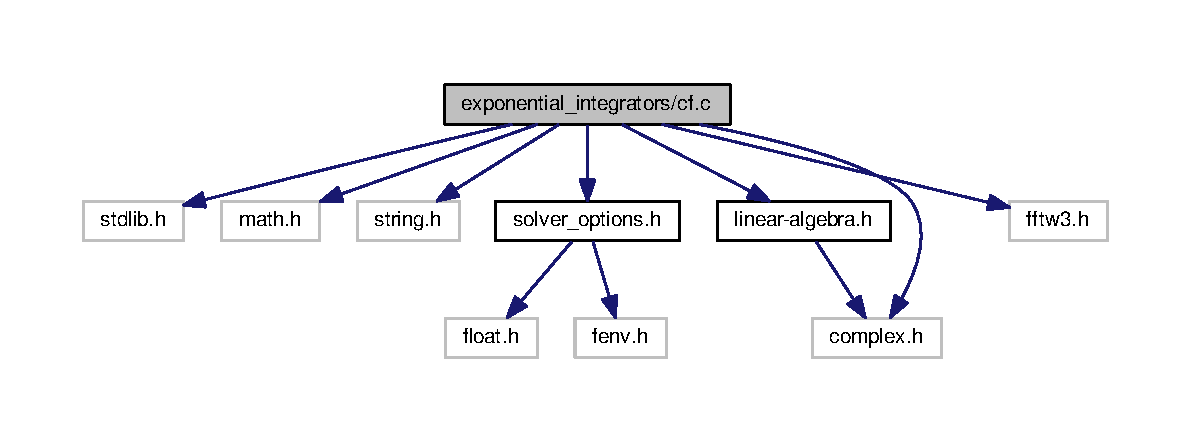
\includegraphics[width=350pt]{cf_8c__incl}
\end{center}
\end{figure}
\subsection*{Macros}
\begin{DoxyCompactItemize}
\item 
\#define \hyperlink{cf_8c_ae71449b1cc6e6250b91f539153a7a0d3}{M\+\_\+\+PI}~4 $\ast$ atan(1)
\end{DoxyCompactItemize}
\subsection*{Functions}
\begin{DoxyCompactItemize}
\item 
void \hyperlink{cf_8c_a8fe7eda5752653bf298684fbe6a18045}{cf} (int n, double $\ast$poles\+\_\+r, double $\ast$poles\+\_\+i, double $\ast$res\+\_\+r, double $\ast$res\+\_\+i)
\begin{DoxyCompactList}\small\item\em Function that calculates the poles and residuals of best rational (partial fraction) approximant to the matrix exponential. \end{DoxyCompactList}\end{DoxyCompactItemize}


\subsection{Detailed Description}
File containing functions for best rational approximation to matrix exponential.

\begin{DoxyAuthor}{Author}
Kyle E. Niemeyer 
\end{DoxyAuthor}
\begin{DoxyDate}{Date}
07/19/2012
\end{DoxyDate}
Contains main and linear algebra functions. 

\subsection{Macro Definition Documentation}
\index{cf.\+c@{cf.\+c}!M\+\_\+\+PI@{M\+\_\+\+PI}}
\index{M\+\_\+\+PI@{M\+\_\+\+PI}!cf.\+c@{cf.\+c}}
\subsubsection[{\texorpdfstring{M\+\_\+\+PI}{M_PI}}]{\setlength{\rightskip}{0pt plus 5cm}\#define M\+\_\+\+PI~4 $\ast$ atan(1)}\hypertarget{cf_8c_ae71449b1cc6e6250b91f539153a7a0d3}{}\label{cf_8c_ae71449b1cc6e6250b91f539153a7a0d3}
Defined for pi 

\subsection{Function Documentation}
\index{cf.\+c@{cf.\+c}!cf@{cf}}
\index{cf@{cf}!cf.\+c@{cf.\+c}}
\subsubsection[{\texorpdfstring{cf(int n, double $\ast$poles\+\_\+r, double $\ast$poles\+\_\+i, double $\ast$res\+\_\+r, double $\ast$res\+\_\+i)}{cf(int n, double *poles_r, double *poles_i, double *res_r, double *res_i)}}]{\setlength{\rightskip}{0pt plus 5cm}void cf (
\begin{DoxyParamCaption}
\item[{int}]{n, }
\item[{double $\ast$}]{poles\+\_\+r, }
\item[{double $\ast$}]{poles\+\_\+i, }
\item[{double $\ast$}]{res\+\_\+r, }
\item[{double $\ast$}]{res\+\_\+i}
\end{DoxyParamCaption}
)}\hypertarget{cf_8c_a8fe7eda5752653bf298684fbe6a18045}{}\label{cf_8c_a8fe7eda5752653bf298684fbe6a18045}


Function that calculates the poles and residuals of best rational (partial fraction) approximant to the matrix exponential. 

Complex math Fast Fourier tranform functions\+Uses the Carathéodory-\/\+Fejér method; based on the M\+A\+T\+L\+AB code in L.\+N. Trefethen, J.\+A.\+C. Weideman, T. Schmelzer, \char`\"{}\+Talbot quadratures
and rational approximations,\char`\"{} B\+IT Numer. Math. 46 (2006) 653–670.


\begin{DoxyParams}[1]{Parameters}
\mbox{\tt in}  & {\em n} & size of approximation (n, n) \\
\hline
\mbox{\tt out}  & {\em poles\+\_\+r} & array with real parts of poles, size n \\
\hline
\mbox{\tt out}  & {\em poles\+\_\+i} & array with imaginary parts of poles, size n \\
\hline
\mbox{\tt out}  & {\em res\+\_\+r} & array with real parts of residuals, size n \\
\hline
\mbox{\tt out}  & {\em res\+\_\+i} & array with imaginary parts of residuals, size n \\
\hline
\end{DoxyParams}

\hypertarget{cf_8h}{}\section{exponential\+\_\+integrators/cf.h File Reference}
\label{cf_8h}\index{exponential\+\_\+integrators/cf.\+h@{exponential\+\_\+integrators/cf.\+h}}
This graph shows which files directly or indirectly include this file\+:
\nopagebreak
\begin{figure}[H]
\begin{center}
\leavevmode
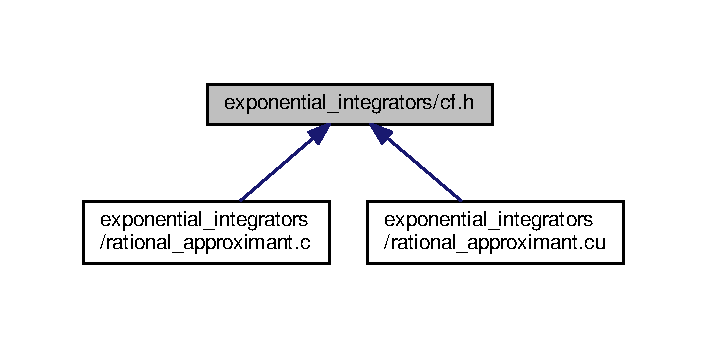
\includegraphics[width=340pt]{cf_8h__dep__incl}
\end{center}
\end{figure}
\subsection*{Functions}
\begin{DoxyCompactItemize}
\item 
void \hyperlink{cf_8h_a23782e739472bc8086465d42bf59bd7b}{cf} (int, double $\ast$, double $\ast$, double $\ast$, double $\ast$)
\begin{DoxyCompactList}\small\item\em Function that calculates the poles and residuals of best rational (partial fraction) approximant to the matrix exponential. \end{DoxyCompactList}\end{DoxyCompactItemize}


\subsection{Function Documentation}
\index{cf.\+h@{cf.\+h}!cf@{cf}}
\index{cf@{cf}!cf.\+h@{cf.\+h}}
\subsubsection[{\texorpdfstring{cf(int, double $\ast$, double $\ast$, double $\ast$, double $\ast$)}{cf(int, double *, double *, double *, double *)}}]{\setlength{\rightskip}{0pt plus 5cm}void cf (
\begin{DoxyParamCaption}
\item[{int}]{n, }
\item[{double $\ast$}]{poles\+\_\+r, }
\item[{double $\ast$}]{poles\+\_\+i, }
\item[{double $\ast$}]{res\+\_\+r, }
\item[{double $\ast$}]{res\+\_\+i}
\end{DoxyParamCaption}
)}\hypertarget{cf_8h_a23782e739472bc8086465d42bf59bd7b}{}\label{cf_8h_a23782e739472bc8086465d42bf59bd7b}


Function that calculates the poles and residuals of best rational (partial fraction) approximant to the matrix exponential. 

Complex math Fast Fourier tranform functions\+Uses the Carathéodory-\/\+Fejér method; based on the M\+A\+T\+L\+AB code in L.\+N. Trefethen, J.\+A.\+C. Weideman, T. Schmelzer, \char`\"{}\+Talbot quadratures
and rational approximations,\char`\"{} B\+IT Numer. Math. 46 (2006) 653–670.


\begin{DoxyParams}[1]{Parameters}
\mbox{\tt in}  & {\em n} & size of approximation (n, n) \\
\hline
\mbox{\tt out}  & {\em poles\+\_\+r} & array with real parts of poles, size n \\
\hline
\mbox{\tt out}  & {\em poles\+\_\+i} & array with imaginary parts of poles, size n \\
\hline
\mbox{\tt out}  & {\em res\+\_\+r} & array with real parts of residuals, size n \\
\hline
\mbox{\tt out}  & {\em res\+\_\+i} & array with imaginary parts of residuals, size n \\
\hline
\end{DoxyParams}

\hypertarget{exp4_8c}{}\section{exponential\+\_\+integrators/exp4/exp4.c File Reference}
\label{exp4_8c}\index{exponential\+\_\+integrators/exp4/exp4.\+c@{exponential\+\_\+integrators/exp4/exp4.\+c}}


A krylov subspace integrator using the fourth-\/order (3rd order embedded) Rosenbrock-\/like solver of Hochbruck et al. (1998)  


{\ttfamily \#include $<$stdlib.\+h$>$}\\*
{\ttfamily \#include $<$stdio.\+h$>$}\\*
{\ttfamily \#include $<$math.\+h$>$}\\*
{\ttfamily \#include $<$stdbool.\+h$>$}\\*
{\ttfamily \#include $<$string.\+h$>$}\\*
{\ttfamily \#include \char`\"{}header.\+h\char`\"{}}\\*
{\ttfamily \#include \char`\"{}dydt.\+h\char`\"{}}\\*
{\ttfamily \#include \char`\"{}jacob.\+h\char`\"{}}\\*
{\ttfamily \#include \char`\"{}arnoldi.\+h\char`\"{}}\\*
{\ttfamily \#include \char`\"{}exp4\+\_\+props.\+h\char`\"{}}\\*
{\ttfamily \#include \char`\"{}exponential\+\_\+linear\+\_\+algebra.\+h\char`\"{}}\\*
{\ttfamily \#include \char`\"{}solver\+\_\+init.\+h\char`\"{}}\\*
{\ttfamily \#include \char`\"{}sparse\+\_\+multiplier.\+h\char`\"{}}\\*
Include dependency graph for exp4.\+c\+:\nopagebreak
\begin{figure}[H]
\begin{center}
\leavevmode
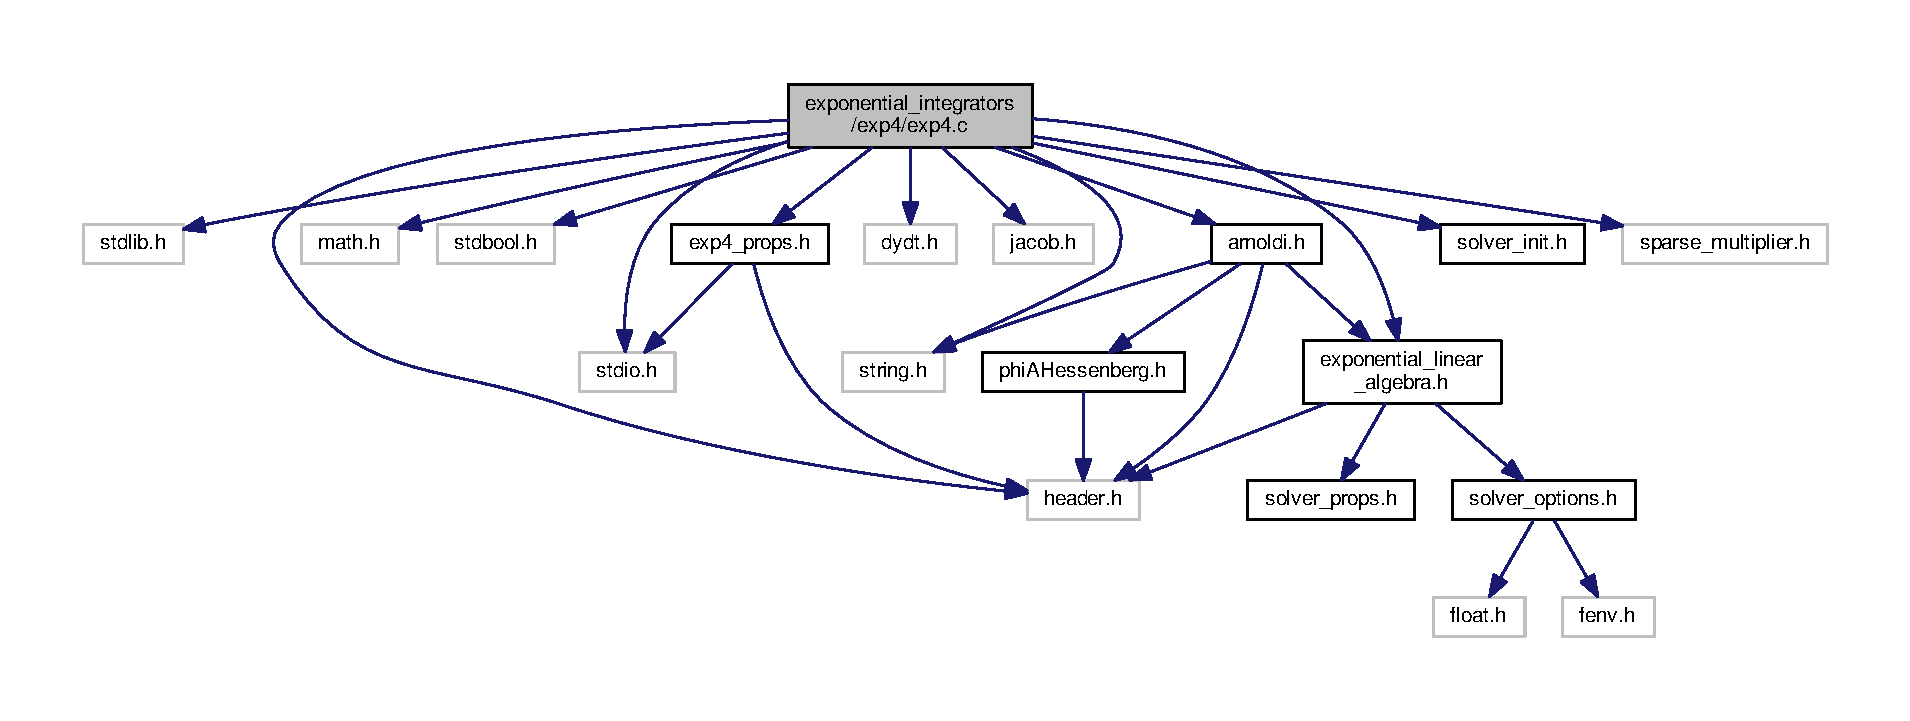
\includegraphics[width=350pt]{exp4_8c__incl}
\end{center}
\end{figure}
\subsection*{Namespaces}
\begin{DoxyCompactItemize}
\item 
 \hyperlink{namespaceexp4}{exp4}
\end{DoxyCompactItemize}
\subsection*{Functions}
\begin{DoxyCompactItemize}
\item 
int \hyperlink{namespaceexp4_a8d03ab917f8736a37474362beeff9391}{exp4\+::integrate} (const double t\+\_\+start, const double t\+\_\+end, const double pr, double $\ast$y)
\begin{DoxyCompactList}\small\item\em 4th-\/order exponential integrator function w/ adaptive Kyrlov subspace approximation \end{DoxyCompactList}\end{DoxyCompactItemize}


\subsection{Detailed Description}
A krylov subspace integrator using the fourth-\/order (3rd order embedded) Rosenbrock-\/like solver of Hochbruck et al. (1998) 

\begin{DoxyAuthor}{Author}
Nicholas J. Curtis 
\end{DoxyAuthor}
\begin{DoxyDate}{Date}
09/02/2014
\end{DoxyDate}
See full reference\+: M. Hochbruck, C. Lubich, H. Selhofer, Exponential integrators for large systems of differential equations, S\+I\+AM J. Sci. Comput. 19 (5) (1998) 1552–1574. doi\+:10.\+1137/\+S1064827595295337

N\+O\+TE\+: all matricies stored in column major format! 
\hypertarget{exp4_8cu}{}\section{exponential\+\_\+integrators/exp4/exp4.cu File Reference}
\label{exp4_8cu}\index{exponential\+\_\+integrators/exp4/exp4.\+cu@{exponential\+\_\+integrators/exp4/exp4.\+cu}}


A krylov subspace integrator using the fourth-\/order (3rd order embedded) Rosenbrock-\/like solver of Hochbruck et al. (1998)  


{\ttfamily \#include $<$stdlib.\+h$>$}\\*
{\ttfamily \#include $<$stdio.\+h$>$}\\*
{\ttfamily \#include $<$math.\+h$>$}\\*
{\ttfamily \#include $<$stdbool.\+h$>$}\\*
{\ttfamily \#include $<$cu\+Complex.\+h$>$}\\*
{\ttfamily \#include \char`\"{}header.\+cuh\char`\"{}}\\*
{\ttfamily \#include \char`\"{}solver\+\_\+options.\+cuh\char`\"{}}\\*
{\ttfamily \#include \char`\"{}solver\+\_\+props.\+cuh\char`\"{}}\\*
{\ttfamily \#include \char`\"{}dydt.\+cuh\char`\"{}}\\*
{\ttfamily \#include \char`\"{}jacob.\+cuh\char`\"{}}\\*
{\ttfamily \#include \char`\"{}arnoldi.\+cuh\char`\"{}}\\*
{\ttfamily \#include \char`\"{}exponential\+\_\+linear\+\_\+algebra.\+cuh\char`\"{}}\\*
{\ttfamily \#include \char`\"{}solver\+\_\+init.\+cuh\char`\"{}}\\*
{\ttfamily \#include \char`\"{}gpu\+\_\+macros.\+cuh\char`\"{}}\\*
Include dependency graph for exp4.\+cu\+:\nopagebreak
\begin{figure}[H]
\begin{center}
\leavevmode
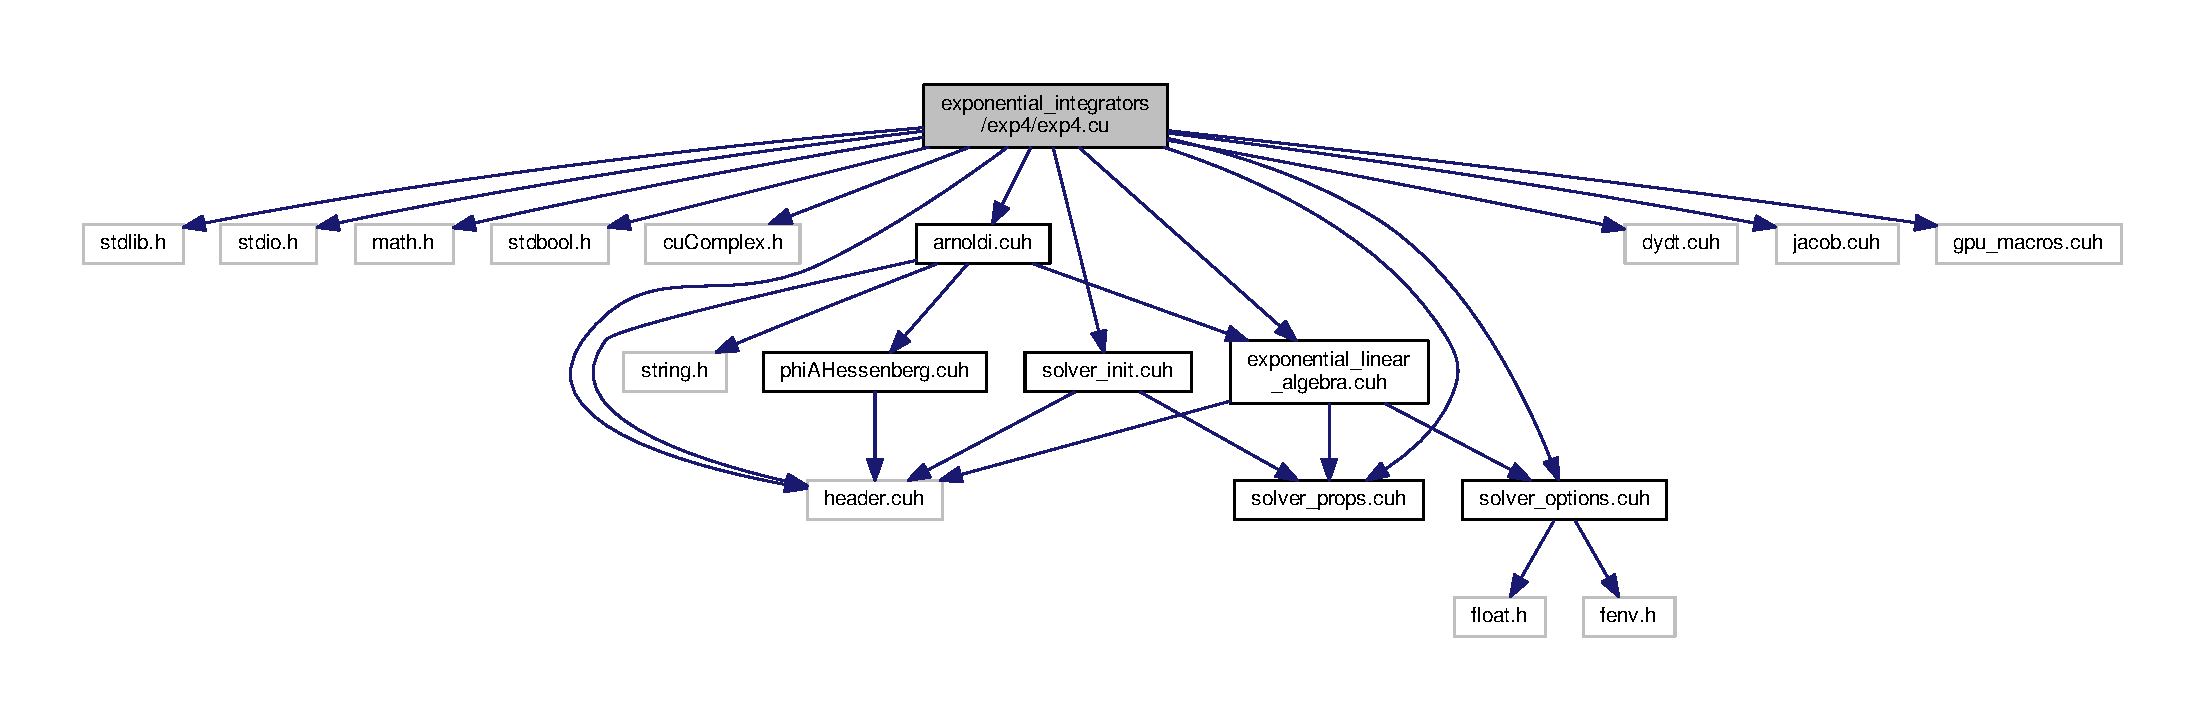
\includegraphics[width=350pt]{exp4_8cu__incl}
\end{center}
\end{figure}
\subsection*{Namespaces}
\begin{DoxyCompactItemize}
\item 
 \hyperlink{namespaceexp4cu}{exp4cu}
\end{DoxyCompactItemize}
\subsection*{Functions}
\begin{DoxyCompactItemize}
\item 
\+\_\+\+\_\+device\+\_\+\+\_\+ void \hyperlink{namespaceexp4cu_aac3abe15ef50061cdfe24ed7d9d64b7a}{exp4cu\+::integrate} (const double t\+\_\+start, const double t\+\_\+end, const double pr, double $\ast$\+\_\+\+\_\+restrict\+\_\+\+\_\+ y, const mechanism\+\_\+memory $\ast$\+\_\+\+\_\+restrict\+\_\+\+\_\+ mech, const \hyperlink{structsolver__memory}{solver\+\_\+memory} $\ast$\+\_\+\+\_\+restrict\+\_\+\+\_\+ solver)
\begin{DoxyCompactList}\small\item\em 4th-\/order exponential integrator function w/ adaptive Kyrlov subspace approximation \end{DoxyCompactList}\end{DoxyCompactItemize}


\subsection{Detailed Description}
A krylov subspace integrator using the fourth-\/order (3rd order embedded) Rosenbrock-\/like solver of Hochbruck et al. (1998) 

\begin{DoxyAuthor}{Author}
Nicholas J. Curtis 
\end{DoxyAuthor}
\begin{DoxyDate}{Date}
09/02/2014
\end{DoxyDate}
See full reference\+: M. Hochbruck, C. Lubich, H. Selhofer, Exponential integrators for large systems of differential equations, S\+I\+AM J. Sci. Comput. 19 (5) (1998) 1552–1574. doi\+:10.\+1137/\+S1064827595295337

N\+O\+TE\+: all matricies stored in column major format!

Implementation of the necessary initialization for the E\+X\+P4 method

\begin{DoxyAuthor}{Author}
Nicholas Curtis 
\end{DoxyAuthor}
\begin{DoxyDate}{Date}
03/09/2015 
\end{DoxyDate}

\hypertarget{exp4__init_8c}{}\section{exponential\+\_\+integrators/exp4/exp4\+\_\+init.c File Reference}
\label{exp4__init_8c}\index{exponential\+\_\+integrators/exp4/exp4\+\_\+init.\+c@{exponential\+\_\+integrators/exp4/exp4\+\_\+init.\+c}}


Implementation of the necessary initialization for the E\+X\+P4 method.  


{\ttfamily \#include \char`\"{}rational\+\_\+approximant.\+h\char`\"{}}\\*
Include dependency graph for exp4\+\_\+init.\+c\+:\nopagebreak
\begin{figure}[H]
\begin{center}
\leavevmode
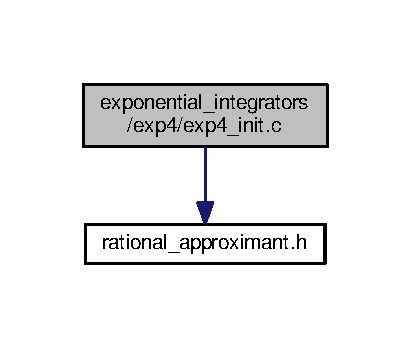
\includegraphics[width=197pt]{exp4__init_8c__incl}
\end{center}
\end{figure}
\subsection*{Namespaces}
\begin{DoxyCompactItemize}
\item 
 \hyperlink{namespaceexp4}{exp4}
\end{DoxyCompactItemize}
\subsection*{Functions}
\begin{DoxyCompactItemize}
\item 
void \hyperlink{namespaceexp4_a1ef7b39a9ac7da4247fd05807f000b07}{exp4\+::init\+\_\+solver\+\_\+log} ()
\begin{DoxyCompactList}\small\item\em Initializes the Krylov subspace logging files (if L\+O\+G\+\_\+\+O\+U\+T\+P\+UT is defined) \end{DoxyCompactList}\item 
void \hyperlink{namespaceexp4_adc563232bff1c62e2068039175a6f428}{exp4\+::solver\+\_\+log} ()
\begin{DoxyCompactList}\small\item\em Executes solver specific logging tasks. \end{DoxyCompactList}\item 
void \hyperlink{namespaceexp4_ab5d3c8262078fd94e511c54eb766f46c}{exp4\+::initialize\+\_\+solver} (int num\+\_\+threads)
\begin{DoxyCompactList}\small\item\em Initializes the solver. \end{DoxyCompactList}\item 
const char $\ast$ \hyperlink{namespaceexp4_aecc47dad1f4379532ab54b896a5e3771}{exp4\+::solver\+\_\+name} ()
\begin{DoxyCompactList}\small\item\em Returns a descriptive solver name. \end{DoxyCompactList}\item 
void \hyperlink{namespaceexp4_a0a595493de14a8f82826268b344339a8}{exp4\+::cleanup\+\_\+solver} (int num\+\_\+threads)
\begin{DoxyCompactList}\small\item\em Cleans up the created solvers. \end{DoxyCompactList}\end{DoxyCompactItemize}


\subsection{Detailed Description}
Implementation of the necessary initialization for the E\+X\+P4 method. 

\begin{DoxyAuthor}{Author}
Nicholas Curtis 
\end{DoxyAuthor}
\begin{DoxyDate}{Date}
03/09/2015 
\end{DoxyDate}

\hypertarget{exp4__init_8cu}{}\section{exponential\+\_\+integrators/exp4/exp4\+\_\+init.cu File Reference}
\label{exp4__init_8cu}\index{exponential\+\_\+integrators/exp4/exp4\+\_\+init.\+cu@{exponential\+\_\+integrators/exp4/exp4\+\_\+init.\+cu}}


Implementation of the necessary initialization for the E\+X\+P4 method.  


{\ttfamily \#include \char`\"{}rational\+\_\+approximant.\+cuh\char`\"{}}\\*
{\ttfamily \#include \char`\"{}solver\+\_\+options.\+cuh\char`\"{}}\\*
{\ttfamily \#include \char`\"{}solver\+\_\+props.\+cuh\char`\"{}}\\*
{\ttfamily \#include \char`\"{}gpu\+\_\+macros.\+cuh\char`\"{}}\\*
Include dependency graph for exp4\+\_\+init.\+cu\+:\nopagebreak
\begin{figure}[H]
\begin{center}
\leavevmode
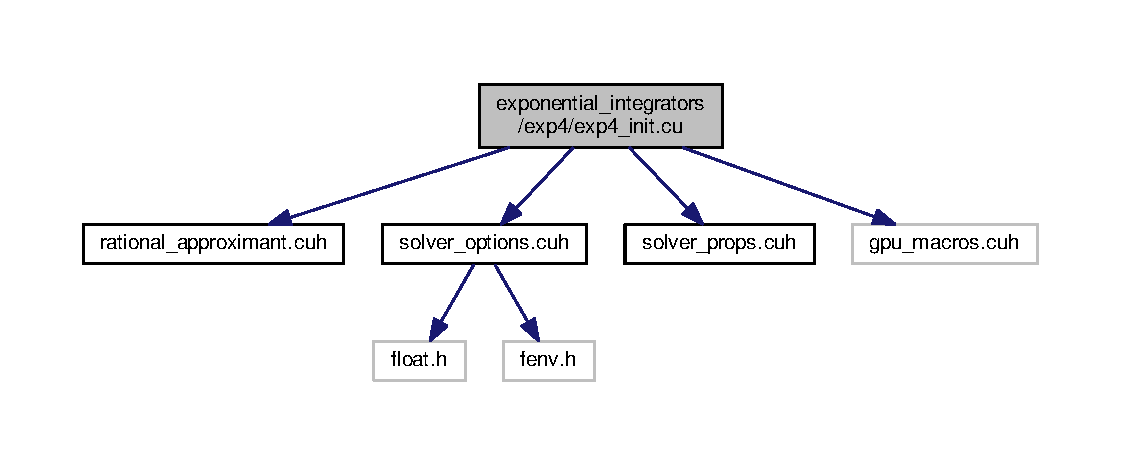
\includegraphics[width=350pt]{exp4__init_8cu__incl}
\end{center}
\end{figure}
\subsection*{Namespaces}
\begin{DoxyCompactItemize}
\item 
 \hyperlink{namespaceexp4cu}{exp4cu}
\end{DoxyCompactItemize}
\subsection*{Functions}
\begin{DoxyCompactItemize}
\item 
void \hyperlink{namespaceexp4cu_abcdabb48b002afcaf4520f85bb06c156}{exp4cu\+::create\+And\+Zero} (void $\ast$$\ast$ptr, size\+\_\+t size)
\begin{DoxyCompactList}\small\item\em Convienvience method to Cuda Malloc and memset a pointer to zero. \end{DoxyCompactList}\item 
void \hyperlink{namespaceexp4cu_aa57e5681ad1b4e46c67d24d12d64e435}{exp4cu\+::initialize\+\_\+solver} (int padded, \hyperlink{structsolver__memory}{solver\+\_\+memory} $\ast$$\ast$h\+\_\+mem, \hyperlink{structsolver__memory}{solver\+\_\+memory} $\ast$$\ast$d\+\_\+mem)
\begin{DoxyCompactList}\small\item\em Initializes the G\+PU solver. \end{DoxyCompactList}\item 
const char $\ast$ \hyperlink{namespaceexp4cu_ad9fad26aa869ef1c6b7fc061e1e6abc3}{exp4cu\+::solver\+\_\+name} ()
\begin{DoxyCompactList}\small\item\em Returns a descriptive solver name. \end{DoxyCompactList}\item 
void \hyperlink{namespaceexp4cu_a042f555823c136890f60ab28454daf9e}{exp4cu\+::solver\+\_\+log} ()
\begin{DoxyCompactList}\small\item\em Executes solver specific logging tasks. \end{DoxyCompactList}\item 
void \hyperlink{namespaceexp4cu_a128b314d7c6b2521bbd64653dc8b9826}{exp4cu\+::init\+\_\+solver\+\_\+log} ()
\begin{DoxyCompactList}\small\item\em Initializes solver specific items for logging. \end{DoxyCompactList}\item 
size\+\_\+t \hyperlink{namespaceexp4cu_a4d5db66ace53978d01e1975e47e30655}{exp4cu\+::required\+\_\+solver\+\_\+size} ()
\begin{DoxyCompactList}\small\item\em Returns the total size (in bytes) required for memory storage for a single G\+PU thread Used in calculation of the maximum number of possible G\+PU threads to launch, this method returns the size of the \hyperlink{structexp4cu_1_1solver__memory}{solver\+\_\+memory} structure (per-\/\+G\+PU thread) \end{DoxyCompactList}\item 
void \hyperlink{namespaceexp4cu_aa775ac1fc1a96522483d9878718cdbf2}{exp4cu\+::cleanup\+\_\+solver} (\hyperlink{structsolver__memory}{solver\+\_\+memory} $\ast$$\ast$h\+\_\+mem, \hyperlink{structsolver__memory}{solver\+\_\+memory} $\ast$$\ast$d\+\_\+mem)
\begin{DoxyCompactList}\small\item\em Cleans up solver memory. \end{DoxyCompactList}\end{DoxyCompactItemize}


\subsection{Detailed Description}
Implementation of the necessary initialization for the E\+X\+P4 method. 

\begin{DoxyAuthor}{Author}
Nicholas Curtis 
\end{DoxyAuthor}
\begin{DoxyDate}{Date}
03/09/2015 
\end{DoxyDate}

\hypertarget{exp4__props_8c}{}\section{exponential\+\_\+integrators/exp4/exp4\+\_\+props.c File Reference}
\label{exp4__props_8c}\index{exponential\+\_\+integrators/exp4/exp4\+\_\+props.\+c@{exponential\+\_\+integrators/exp4/exp4\+\_\+props.\+c}}


Contains error checking for E\+X\+P4 return codes.  


{\ttfamily \#include \char`\"{}exp4\+\_\+props.\+h\char`\"{}}\\*
Include dependency graph for exp4\+\_\+props.\+c\+:\nopagebreak
\begin{figure}[H]
\begin{center}
\leavevmode
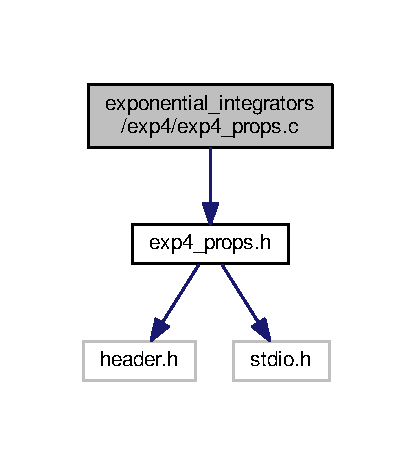
\includegraphics[width=200pt]{exp4__props_8c__incl}
\end{center}
\end{figure}
\subsection*{Namespaces}
\begin{DoxyCompactItemize}
\item 
 \hyperlink{namespaceexp4}{exp4}
\end{DoxyCompactItemize}
\subsection*{Functions}
\begin{DoxyCompactItemize}
\item 
void \hyperlink{namespaceexp4_a40f949e51fd1c796b23f6d81612720fb}{exp4\+::check\+\_\+error} (int tid, int code)
\begin{DoxyCompactList}\small\item\em Checks the return code of the given thread (I\+VP) for an error, and exits if found. \end{DoxyCompactList}\end{DoxyCompactItemize}


\subsection{Detailed Description}
Contains error checking for E\+X\+P4 return codes. 

\begin{DoxyAuthor}{Author}
Nicholas J. Curtis 
\end{DoxyAuthor}
\begin{DoxyDate}{Date}
09/02/2014 
\end{DoxyDate}

\hypertarget{exp4__props_8cu}{}\section{exponential\+\_\+integrators/exp4/exp4\+\_\+props.cu File Reference}
\label{exp4__props_8cu}\index{exponential\+\_\+integrators/exp4/exp4\+\_\+props.\+cu@{exponential\+\_\+integrators/exp4/exp4\+\_\+props.\+cu}}


Error checking for the E\+X\+P4 algorithm.  


{\ttfamily \#include \char`\"{}exp4\+\_\+props.\+cuh\char`\"{}}\\*
Include dependency graph for exp4\+\_\+props.\+cu\+:\nopagebreak
\begin{figure}[H]
\begin{center}
\leavevmode
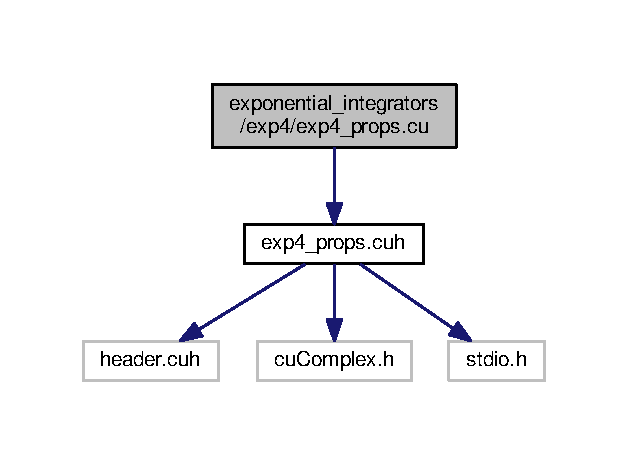
\includegraphics[width=302pt]{exp4__props_8cu__incl}
\end{center}
\end{figure}
\subsection*{Namespaces}
\begin{DoxyCompactItemize}
\item 
 \hyperlink{namespaceexp4cu}{exp4cu}
\end{DoxyCompactItemize}
\subsection*{Functions}
\begin{DoxyCompactItemize}
\item 
\+\_\+\+\_\+host\+\_\+\+\_\+ void \hyperlink{namespaceexp4cu_a2d5234f5e9971aec336ac64ce719f1f4}{exp4cu\+::check\+\_\+error} (int num\+\_\+cond, int $\ast$codes)
\end{DoxyCompactItemize}


\subsection{Detailed Description}
Error checking for the E\+X\+P4 algorithm. 

\begin{DoxyAuthor}{Author}
Nicholas Curtis 
\end{DoxyAuthor}
\begin{DoxyDate}{Date}
03/10/2015 
\end{DoxyDate}

\hypertarget{exp4__props_8cuh}{}\section{exponential\+\_\+integrators/exp4/exp4\+\_\+props.cuh File Reference}
\label{exp4__props_8cuh}\index{exponential\+\_\+integrators/exp4/exp4\+\_\+props.\+cuh@{exponential\+\_\+integrators/exp4/exp4\+\_\+props.\+cuh}}


Error checking for the E\+X\+P4 algorithm.  


{\ttfamily \#include \char`\"{}header.\+cuh\char`\"{}}\\*
{\ttfamily \#include $<$cu\+Complex.\+h$>$}\\*
{\ttfamily \#include $<$stdio.\+h$>$}\\*
Include dependency graph for exp4\+\_\+props.\+cuh\+:\nopagebreak
\begin{figure}[H]
\begin{center}
\leavevmode
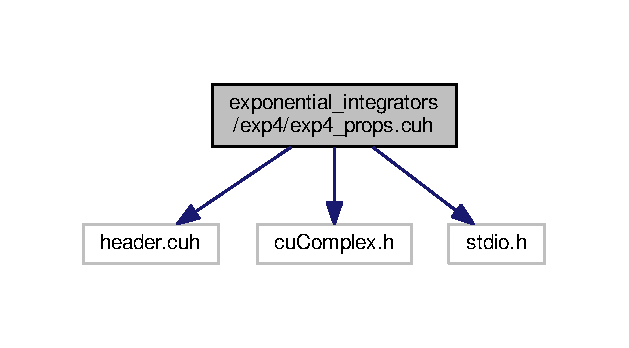
\includegraphics[width=302pt]{exp4__props_8cuh__incl}
\end{center}
\end{figure}
This graph shows which files directly or indirectly include this file\+:\nopagebreak
\begin{figure}[H]
\begin{center}
\leavevmode
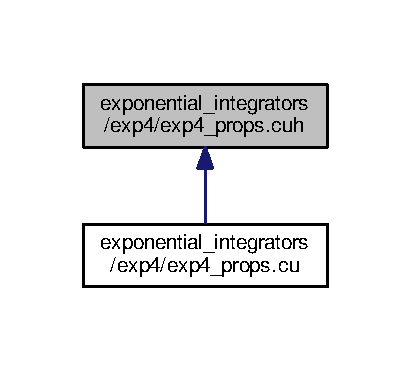
\includegraphics[width=197pt]{exp4__props_8cuh__dep__incl}
\end{center}
\end{figure}
\subsection*{Classes}
\begin{DoxyCompactItemize}
\item 
struct \hyperlink{structexp4cu_1_1solver__memory}{exp4cu\+::solver\+\_\+memory}
\begin{DoxyCompactList}\small\item\em Structure containing memory needed for E\+X\+P4 algorithm. \end{DoxyCompactList}\end{DoxyCompactItemize}
\subsection*{Namespaces}
\begin{DoxyCompactItemize}
\item 
 \hyperlink{namespaceexp4cu}{exp4cu}
\end{DoxyCompactItemize}
\subsection*{Macros}
\begin{DoxyCompactItemize}
\item 
\#define \hyperlink{exp4__props_8cuh_a012706e43fb2a3e4102cae6222cccf91}{E\+X\+P4\+\_\+\+P\+R\+O\+P\+S\+\_\+\+C\+UH}
\item 
\#define \hyperlink{exp4__props_8cuh_a2748566f4c443ee77aa831e63dbb5ebe}{P}~1
\begin{DoxyCompactList}\small\item\em max order of the phi functions (for error estimation) \end{DoxyCompactList}\item 
\#define \hyperlink{exp4__props_8cuh_ac5232262b17b940a7b54e6e56439aa24}{O\+RD}~3.\+0
\begin{DoxyCompactList}\small\item\em order of embedded methods \end{DoxyCompactList}\item 
\#define \hyperlink{exp4__props_8cuh_a61819141b0164a35f4d791b0e696721f}{M\+\_\+\+M\+AX}~N\+SP
\begin{DoxyCompactList}\small\item\em maximum Krylov dimension (without phi order) \end{DoxyCompactList}\item 
\#define \hyperlink{exp4__props_8cuh_a351d54267048643c4365f6a24641d0cf}{S\+T\+R\+I\+DE}~(\hyperlink{exprb43__props_8h_a61819141b0164a35f4d791b0e696721f}{M\+\_\+\+M\+AX} + \hyperlink{exprb43__props_8h_a2748566f4c443ee77aa831e63dbb5ebe}{P})
\begin{DoxyCompactList}\small\item\em Krylov matrix stride. \end{DoxyCompactList}\item 
\#define \hyperlink{exp4__props_8cuh_aa0414caef00a64a51d4c6c0711d9e70a}{M\+A\+X\+\_\+\+S\+T\+E\+PS}~(10000)
\begin{DoxyCompactList}\small\item\em Maximum allowed internal timesteps per integration step. \end{DoxyCompactList}\item 
\#define \hyperlink{exp4__props_8cuh_a0f51553c710580b9899756f7ad472c93}{M\+A\+X\+\_\+\+C\+O\+N\+S\+E\+C\+U\+T\+I\+V\+E\+\_\+\+E\+R\+R\+O\+RS}~(5)
\begin{DoxyCompactList}\small\item\em Number of consecutive errors on internal integration steps allowed before exit. \end{DoxyCompactList}\item 
\#define \hyperlink{group__exp4cu__ErrCodes_gabd83bc0f9f475a2189a4db4a08b790ca}{E\+C\+\_\+success}~(0)
\begin{DoxyCompactList}\small\item\em Successful integration step. \end{DoxyCompactList}\item 
\#define \hyperlink{group__exp4cu__ErrCodes_gae0287841c08f86f5709660fd731615ad}{E\+C\+\_\+consecutive\+\_\+steps}~(1)
\begin{DoxyCompactList}\small\item\em Maximum consecutive errors on internal integration steps reached. \end{DoxyCompactList}\item 
\#define \hyperlink{group__exp4cu__ErrCodes_ga0f0275d9851ab5c19b79a963d5084df3}{E\+C\+\_\+max\+\_\+steps\+\_\+exceeded}~(2)
\begin{DoxyCompactList}\small\item\em Maximum number of internal integration steps reached. \end{DoxyCompactList}\item 
\#define \hyperlink{group__exp4cu__ErrCodes_ga9326efd544880e2683c4453365ca2704}{E\+C\+\_\+h\+\_\+plus\+\_\+t\+\_\+equals\+\_\+h}~(3)
\begin{DoxyCompactList}\small\item\em Timestep reduced such that update would have no effect on simulation time. \end{DoxyCompactList}\end{DoxyCompactItemize}


\subsection{Detailed Description}
Error checking for the E\+X\+P4 algorithm. 

Various macros controlling behaviour of E\+X\+P4 algorithm.

\begin{DoxyAuthor}{Author}
Nicholas Curtis 
\end{DoxyAuthor}
\begin{DoxyDate}{Date}
03/10/2015 
\end{DoxyDate}


\subsection{Macro Definition Documentation}
\index{exp4\+\_\+props.\+cuh@{exp4\+\_\+props.\+cuh}!E\+X\+P4\+\_\+\+P\+R\+O\+P\+S\+\_\+\+C\+UH@{E\+X\+P4\+\_\+\+P\+R\+O\+P\+S\+\_\+\+C\+UH}}
\index{E\+X\+P4\+\_\+\+P\+R\+O\+P\+S\+\_\+\+C\+UH@{E\+X\+P4\+\_\+\+P\+R\+O\+P\+S\+\_\+\+C\+UH}!exp4\+\_\+props.\+cuh@{exp4\+\_\+props.\+cuh}}
\subsubsection[{\texorpdfstring{E\+X\+P4\+\_\+\+P\+R\+O\+P\+S\+\_\+\+C\+UH}{EXP4_PROPS_CUH}}]{\setlength{\rightskip}{0pt plus 5cm}\#define E\+X\+P4\+\_\+\+P\+R\+O\+P\+S\+\_\+\+C\+UH}\hypertarget{exp4__props_8cuh_a012706e43fb2a3e4102cae6222cccf91}{}\label{exp4__props_8cuh_a012706e43fb2a3e4102cae6222cccf91}
\index{exp4\+\_\+props.\+cuh@{exp4\+\_\+props.\+cuh}!M\+\_\+\+M\+AX@{M\+\_\+\+M\+AX}}
\index{M\+\_\+\+M\+AX@{M\+\_\+\+M\+AX}!exp4\+\_\+props.\+cuh@{exp4\+\_\+props.\+cuh}}
\subsubsection[{\texorpdfstring{M\+\_\+\+M\+AX}{M_MAX}}]{\setlength{\rightskip}{0pt plus 5cm}\#define M\+\_\+\+M\+AX~N\+SP}\hypertarget{exp4__props_8cuh_a61819141b0164a35f4d791b0e696721f}{}\label{exp4__props_8cuh_a61819141b0164a35f4d791b0e696721f}


maximum Krylov dimension (without phi order) 

\index{exp4\+\_\+props.\+cuh@{exp4\+\_\+props.\+cuh}!M\+A\+X\+\_\+\+C\+O\+N\+S\+E\+C\+U\+T\+I\+V\+E\+\_\+\+E\+R\+R\+O\+RS@{M\+A\+X\+\_\+\+C\+O\+N\+S\+E\+C\+U\+T\+I\+V\+E\+\_\+\+E\+R\+R\+O\+RS}}
\index{M\+A\+X\+\_\+\+C\+O\+N\+S\+E\+C\+U\+T\+I\+V\+E\+\_\+\+E\+R\+R\+O\+RS@{M\+A\+X\+\_\+\+C\+O\+N\+S\+E\+C\+U\+T\+I\+V\+E\+\_\+\+E\+R\+R\+O\+RS}!exp4\+\_\+props.\+cuh@{exp4\+\_\+props.\+cuh}}
\subsubsection[{\texorpdfstring{M\+A\+X\+\_\+\+C\+O\+N\+S\+E\+C\+U\+T\+I\+V\+E\+\_\+\+E\+R\+R\+O\+RS}{MAX_CONSECUTIVE_ERRORS}}]{\setlength{\rightskip}{0pt plus 5cm}\#define M\+A\+X\+\_\+\+C\+O\+N\+S\+E\+C\+U\+T\+I\+V\+E\+\_\+\+E\+R\+R\+O\+RS~(5)}\hypertarget{exp4__props_8cuh_a0f51553c710580b9899756f7ad472c93}{}\label{exp4__props_8cuh_a0f51553c710580b9899756f7ad472c93}


Number of consecutive errors on internal integration steps allowed before exit. 

\index{exp4\+\_\+props.\+cuh@{exp4\+\_\+props.\+cuh}!M\+A\+X\+\_\+\+S\+T\+E\+PS@{M\+A\+X\+\_\+\+S\+T\+E\+PS}}
\index{M\+A\+X\+\_\+\+S\+T\+E\+PS@{M\+A\+X\+\_\+\+S\+T\+E\+PS}!exp4\+\_\+props.\+cuh@{exp4\+\_\+props.\+cuh}}
\subsubsection[{\texorpdfstring{M\+A\+X\+\_\+\+S\+T\+E\+PS}{MAX_STEPS}}]{\setlength{\rightskip}{0pt plus 5cm}\#define M\+A\+X\+\_\+\+S\+T\+E\+PS~(10000)}\hypertarget{exp4__props_8cuh_aa0414caef00a64a51d4c6c0711d9e70a}{}\label{exp4__props_8cuh_aa0414caef00a64a51d4c6c0711d9e70a}


Maximum allowed internal timesteps per integration step. 

\index{exp4\+\_\+props.\+cuh@{exp4\+\_\+props.\+cuh}!O\+RD@{O\+RD}}
\index{O\+RD@{O\+RD}!exp4\+\_\+props.\+cuh@{exp4\+\_\+props.\+cuh}}
\subsubsection[{\texorpdfstring{O\+RD}{ORD}}]{\setlength{\rightskip}{0pt plus 5cm}\#define O\+RD~3.\+0}\hypertarget{exp4__props_8cuh_ac5232262b17b940a7b54e6e56439aa24}{}\label{exp4__props_8cuh_ac5232262b17b940a7b54e6e56439aa24}


order of embedded methods 

\index{exp4\+\_\+props.\+cuh@{exp4\+\_\+props.\+cuh}!P@{P}}
\index{P@{P}!exp4\+\_\+props.\+cuh@{exp4\+\_\+props.\+cuh}}
\subsubsection[{\texorpdfstring{P}{P}}]{\setlength{\rightskip}{0pt plus 5cm}\#define P~1}\hypertarget{exp4__props_8cuh_a2748566f4c443ee77aa831e63dbb5ebe}{}\label{exp4__props_8cuh_a2748566f4c443ee77aa831e63dbb5ebe}


max order of the phi functions (for error estimation) 

\index{exp4\+\_\+props.\+cuh@{exp4\+\_\+props.\+cuh}!S\+T\+R\+I\+DE@{S\+T\+R\+I\+DE}}
\index{S\+T\+R\+I\+DE@{S\+T\+R\+I\+DE}!exp4\+\_\+props.\+cuh@{exp4\+\_\+props.\+cuh}}
\subsubsection[{\texorpdfstring{S\+T\+R\+I\+DE}{STRIDE}}]{\setlength{\rightskip}{0pt plus 5cm}\#define S\+T\+R\+I\+DE~({\bf M\+\_\+\+M\+AX} + {\bf P})}\hypertarget{exp4__props_8cuh_a351d54267048643c4365f6a24641d0cf}{}\label{exp4__props_8cuh_a351d54267048643c4365f6a24641d0cf}


Krylov matrix stride. 


\hypertarget{exp4__props_8h}{}\section{/home/nick/\+Dropbox/acceler\+Int/exponential\+\_\+integrators/exp4/exp4\+\_\+props.h File Reference}
\label{exp4__props_8h}\index{/home/nick/\+Dropbox/acceler\+Int/exponential\+\_\+integrators/exp4/exp4\+\_\+props.\+h@{/home/nick/\+Dropbox/acceler\+Int/exponential\+\_\+integrators/exp4/exp4\+\_\+props.\+h}}


Various macros controlling behaviour of E\+X\+P4 algorithm.  


{\ttfamily \#include \char`\"{}header.\+h\char`\"{}}\\*
{\ttfamily \#include $<$stdio.\+h$>$}\\*
Include dependency graph for exp4\+\_\+props.\+h\+:
\nopagebreak
\begin{figure}[H]
\begin{center}
\leavevmode
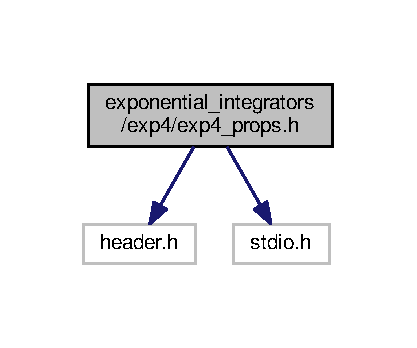
\includegraphics[width=199pt]{exp4__props_8h__incl}
\end{center}
\end{figure}
This graph shows which files directly or indirectly include this file\+:
\nopagebreak
\begin{figure}[H]
\begin{center}
\leavevmode
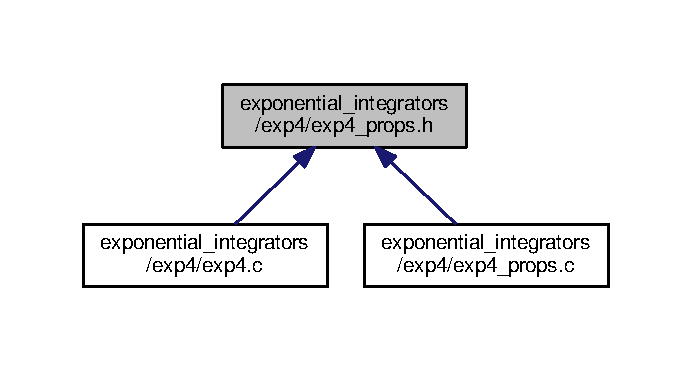
\includegraphics[width=338pt]{exp4__props_8h__dep__incl}
\end{center}
\end{figure}
\subsection*{Namespaces}
\begin{DoxyCompactItemize}
\item 
 \hyperlink{namespaceexp4}{exp4}
\end{DoxyCompactItemize}
\subsection*{Macros}
\begin{DoxyCompactItemize}
\item 
\#define \hyperlink{exp4__props_8h_a2748566f4c443ee77aa831e63dbb5ebe}{P}~1
\begin{DoxyCompactList}\small\item\em max order of the phi functions (for error estimation) \end{DoxyCompactList}\item 
\#define \hyperlink{exp4__props_8h_ac5232262b17b940a7b54e6e56439aa24}{O\+RD}~3.\+0
\begin{DoxyCompactList}\small\item\em order of embedded methods \end{DoxyCompactList}\item 
\#define \hyperlink{exp4__props_8h_a61819141b0164a35f4d791b0e696721f}{M\+\_\+\+M\+AX}~N\+SP
\begin{DoxyCompactList}\small\item\em maximum Krylov dimension (without phi order) \end{DoxyCompactList}\item 
\#define \hyperlink{exp4__props_8h_a351d54267048643c4365f6a24641d0cf}{S\+T\+R\+I\+DE}~(\hyperlink{exprb43__props_8h_a61819141b0164a35f4d791b0e696721f}{M\+\_\+\+M\+AX} + \hyperlink{exprb43__props_8h_a2748566f4c443ee77aa831e63dbb5ebe}{P})
\begin{DoxyCompactList}\small\item\em Krylov matrix stride. \end{DoxyCompactList}\item 
\#define \hyperlink{exp4__props_8h_aa0414caef00a64a51d4c6c0711d9e70a}{M\+A\+X\+\_\+\+S\+T\+E\+PS}~(100000)
\begin{DoxyCompactList}\small\item\em Maximum allowed internal timesteps per integration step. \end{DoxyCompactList}\item 
\#define \hyperlink{exp4__props_8h_a0f51553c710580b9899756f7ad472c93}{M\+A\+X\+\_\+\+C\+O\+N\+S\+E\+C\+U\+T\+I\+V\+E\+\_\+\+E\+R\+R\+O\+RS}~(5)
\begin{DoxyCompactList}\small\item\em Number of consecutive errors on internal integration steps allowed before exit. \end{DoxyCompactList}\item 
\#define \hyperlink{group__exp4__ErrCodes_gabd83bc0f9f475a2189a4db4a08b790ca}{E\+C\+\_\+success}~(0)
\begin{DoxyCompactList}\small\item\em Successful integration step. \end{DoxyCompactList}\item 
\#define \hyperlink{group__exp4__ErrCodes_gae0287841c08f86f5709660fd731615ad}{E\+C\+\_\+consecutive\+\_\+steps}~(1)
\begin{DoxyCompactList}\small\item\em Maximum consecutive errors on internal integration steps reached. \end{DoxyCompactList}\item 
\#define \hyperlink{group__exp4__ErrCodes_ga0f0275d9851ab5c19b79a963d5084df3}{E\+C\+\_\+max\+\_\+steps\+\_\+exceeded}~(2)
\begin{DoxyCompactList}\small\item\em Maximum number of internal integration steps reached. \end{DoxyCompactList}\item 
\#define \hyperlink{group__exp4__ErrCodes_ga9326efd544880e2683c4453365ca2704}{E\+C\+\_\+h\+\_\+plus\+\_\+t\+\_\+equals\+\_\+h}~(3)
\begin{DoxyCompactList}\small\item\em Timestep reduced such that update would have no effect on simulation time. \end{DoxyCompactList}\end{DoxyCompactItemize}


\subsection{Detailed Description}
Various macros controlling behaviour of E\+X\+P4 algorithm. 

\begin{DoxyAuthor}{Author}
Nicholas Curtis 
\end{DoxyAuthor}
\begin{DoxyDate}{Date}
03/10/2015 
\end{DoxyDate}


\subsection{Macro Definition Documentation}
\index{exp4\+\_\+props.\+h@{exp4\+\_\+props.\+h}!M\+\_\+\+M\+AX@{M\+\_\+\+M\+AX}}
\index{M\+\_\+\+M\+AX@{M\+\_\+\+M\+AX}!exp4\+\_\+props.\+h@{exp4\+\_\+props.\+h}}
\subsubsection[{\texorpdfstring{M\+\_\+\+M\+AX}{M_MAX}}]{\setlength{\rightskip}{0pt plus 5cm}\#define M\+\_\+\+M\+AX~N\+SP}\hypertarget{exp4__props_8h_a61819141b0164a35f4d791b0e696721f}{}\label{exp4__props_8h_a61819141b0164a35f4d791b0e696721f}


maximum Krylov dimension (without phi order) 

\index{exp4\+\_\+props.\+h@{exp4\+\_\+props.\+h}!M\+A\+X\+\_\+\+C\+O\+N\+S\+E\+C\+U\+T\+I\+V\+E\+\_\+\+E\+R\+R\+O\+RS@{M\+A\+X\+\_\+\+C\+O\+N\+S\+E\+C\+U\+T\+I\+V\+E\+\_\+\+E\+R\+R\+O\+RS}}
\index{M\+A\+X\+\_\+\+C\+O\+N\+S\+E\+C\+U\+T\+I\+V\+E\+\_\+\+E\+R\+R\+O\+RS@{M\+A\+X\+\_\+\+C\+O\+N\+S\+E\+C\+U\+T\+I\+V\+E\+\_\+\+E\+R\+R\+O\+RS}!exp4\+\_\+props.\+h@{exp4\+\_\+props.\+h}}
\subsubsection[{\texorpdfstring{M\+A\+X\+\_\+\+C\+O\+N\+S\+E\+C\+U\+T\+I\+V\+E\+\_\+\+E\+R\+R\+O\+RS}{MAX_CONSECUTIVE_ERRORS}}]{\setlength{\rightskip}{0pt plus 5cm}\#define M\+A\+X\+\_\+\+C\+O\+N\+S\+E\+C\+U\+T\+I\+V\+E\+\_\+\+E\+R\+R\+O\+RS~(5)}\hypertarget{exp4__props_8h_a0f51553c710580b9899756f7ad472c93}{}\label{exp4__props_8h_a0f51553c710580b9899756f7ad472c93}


Number of consecutive errors on internal integration steps allowed before exit. 

\index{exp4\+\_\+props.\+h@{exp4\+\_\+props.\+h}!M\+A\+X\+\_\+\+S\+T\+E\+PS@{M\+A\+X\+\_\+\+S\+T\+E\+PS}}
\index{M\+A\+X\+\_\+\+S\+T\+E\+PS@{M\+A\+X\+\_\+\+S\+T\+E\+PS}!exp4\+\_\+props.\+h@{exp4\+\_\+props.\+h}}
\subsubsection[{\texorpdfstring{M\+A\+X\+\_\+\+S\+T\+E\+PS}{MAX_STEPS}}]{\setlength{\rightskip}{0pt plus 5cm}\#define M\+A\+X\+\_\+\+S\+T\+E\+PS~(100000)}\hypertarget{exp4__props_8h_aa0414caef00a64a51d4c6c0711d9e70a}{}\label{exp4__props_8h_aa0414caef00a64a51d4c6c0711d9e70a}


Maximum allowed internal timesteps per integration step. 

\index{exp4\+\_\+props.\+h@{exp4\+\_\+props.\+h}!O\+RD@{O\+RD}}
\index{O\+RD@{O\+RD}!exp4\+\_\+props.\+h@{exp4\+\_\+props.\+h}}
\subsubsection[{\texorpdfstring{O\+RD}{ORD}}]{\setlength{\rightskip}{0pt plus 5cm}\#define O\+RD~3.\+0}\hypertarget{exp4__props_8h_ac5232262b17b940a7b54e6e56439aa24}{}\label{exp4__props_8h_ac5232262b17b940a7b54e6e56439aa24}


order of embedded methods 

\index{exp4\+\_\+props.\+h@{exp4\+\_\+props.\+h}!P@{P}}
\index{P@{P}!exp4\+\_\+props.\+h@{exp4\+\_\+props.\+h}}
\subsubsection[{\texorpdfstring{P}{P}}]{\setlength{\rightskip}{0pt plus 5cm}\#define P~1}\hypertarget{exp4__props_8h_a2748566f4c443ee77aa831e63dbb5ebe}{}\label{exp4__props_8h_a2748566f4c443ee77aa831e63dbb5ebe}


max order of the phi functions (for error estimation) 

\index{exp4\+\_\+props.\+h@{exp4\+\_\+props.\+h}!S\+T\+R\+I\+DE@{S\+T\+R\+I\+DE}}
\index{S\+T\+R\+I\+DE@{S\+T\+R\+I\+DE}!exp4\+\_\+props.\+h@{exp4\+\_\+props.\+h}}
\subsubsection[{\texorpdfstring{S\+T\+R\+I\+DE}{STRIDE}}]{\setlength{\rightskip}{0pt plus 5cm}\#define S\+T\+R\+I\+DE~({\bf M\+\_\+\+M\+AX} + {\bf P})}\hypertarget{exp4__props_8h_a351d54267048643c4365f6a24641d0cf}{}\label{exp4__props_8h_a351d54267048643c4365f6a24641d0cf}


Krylov matrix stride. 


\hypertarget{exponential__linear__algebra_8cu}{}\section{exponential\+\_\+integrators/exponential\+\_\+linear\+\_\+algebra.cu File Reference}
\label{exponential__linear__algebra_8cu}\index{exponential\+\_\+integrators/exponential\+\_\+linear\+\_\+algebra.\+cu@{exponential\+\_\+integrators/exponential\+\_\+linear\+\_\+algebra.\+cu}}


Implementation of various linear algebra functions needed in the exponential integrators.  


{\ttfamily \#include \char`\"{}exponential\+\_\+linear\+\_\+algebra.\+cuh\char`\"{}}\\*
Include dependency graph for exponential\+\_\+linear\+\_\+algebra.\+cu\+:\nopagebreak
\begin{figure}[H]
\begin{center}
\leavevmode
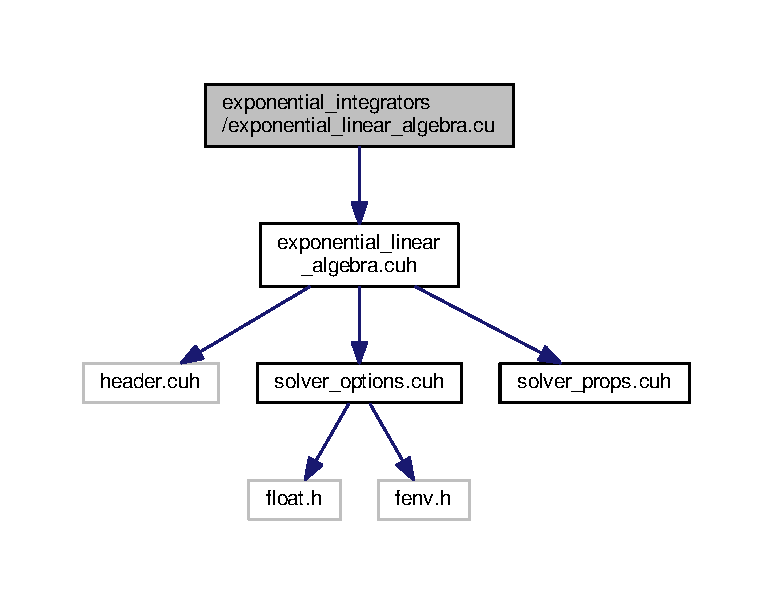
\includegraphics[width=350pt]{exponential__linear__algebra_8cu__incl}
\end{center}
\end{figure}
\subsection*{Functions}
\begin{DoxyCompactItemize}
\item 
\+\_\+\+\_\+device\+\_\+\+\_\+ void \hyperlink{exponential__linear__algebra_8cu_a2e59348b99908b5918de88097e15d5ff}{matvec\+\_\+m\+\_\+by\+\_\+m} (const int m, const double $\ast$const \+\_\+\+\_\+restrict\+\_\+\+\_\+ A, const double $\ast$const \+\_\+\+\_\+restrict\+\_\+\+\_\+ V, double $\ast$const \+\_\+\+\_\+restrict\+\_\+\+\_\+ Av)
\begin{DoxyCompactList}\small\item\em Matrix-\/vector multiplication of a matrix sized MxM and a vector Mx1. \end{DoxyCompactList}\item 
\+\_\+\+\_\+device\+\_\+\+\_\+ void \hyperlink{exponential__linear__algebra_8cu_a6bc7e5c08b8e40b19ce05ea146c05307}{matvec\+\_\+m\+\_\+by\+\_\+m\+\_\+plusequal} (const int m, const double $\ast$const \+\_\+\+\_\+restrict\+\_\+\+\_\+ A, const double $\ast$const \+\_\+\+\_\+restrict\+\_\+\+\_\+ V, double $\ast$const \+\_\+\+\_\+restrict\+\_\+\+\_\+ Av)
\begin{DoxyCompactList}\small\item\em Matrix-\/vector plus equals for a matrix of size MxM and vector of size Mx1. That is, it returns (A + I) $\ast$ v. \end{DoxyCompactList}\item 
\+\_\+\+\_\+device\+\_\+\+\_\+ void \hyperlink{exponential__linear__algebra_8cu_a03e37312683db492dc73e08c17fe40e7}{matvec\+\_\+n\+\_\+by\+\_\+m\+\_\+scale} (const int m, const double \hyperlink{inverse_8cu_adbb4f3f3af5f968a94f717729803c88d}{scale}, const double $\ast$const \+\_\+\+\_\+restrict\+\_\+\+\_\+ A, const double $\ast$const \+\_\+\+\_\+restrict\+\_\+\+\_\+ V, double $\ast$const \+\_\+\+\_\+restrict\+\_\+\+\_\+ Av)
\begin{DoxyCompactList}\small\item\em Matrix-\/vector multiplication of a matrix sized N\+S\+PxM and a vector of size Mx1 scaled by a specified factor That is, it returns A $\ast$ v $\ast$ scale. \end{DoxyCompactList}\item 
\+\_\+\+\_\+device\+\_\+\+\_\+ void \hyperlink{exponential__linear__algebra_8cu_aafe924c72a847b1d591e8fecb0efebdc}{matvec\+\_\+n\+\_\+by\+\_\+m\+\_\+scale\+\_\+special} (const int m, const double $\ast$\+\_\+\+\_\+restrict\+\_\+\+\_\+ \hyperlink{inverse_8cu_adbb4f3f3af5f968a94f717729803c88d}{scale}, const double $\ast$\+\_\+\+\_\+restrict\+\_\+\+\_\+ A, double $\ast$const \+\_\+\+\_\+restrict\+\_\+\+\_\+ $\ast$V, double $\ast$\+\_\+\+\_\+restrict\+\_\+\+\_\+ $\ast$Av)
\begin{DoxyCompactList}\small\item\em Matrix-\/vector multiplication of a matrix sized N\+S\+PxM and a vector of size Mx1 scaled by a specified factor. \end{DoxyCompactList}\item 
\+\_\+\+\_\+device\+\_\+\+\_\+ void \hyperlink{exponential__linear__algebra_8cu_a6d511f330da8ea1a044ed327a132d290}{matvec\+\_\+n\+\_\+by\+\_\+m\+\_\+scale\+\_\+special2} (const int m, const double $\ast$\+\_\+\+\_\+restrict\+\_\+\+\_\+ \hyperlink{inverse_8cu_adbb4f3f3af5f968a94f717729803c88d}{scale}, const double $\ast$\+\_\+\+\_\+restrict\+\_\+\+\_\+ A, double $\ast$const \+\_\+\+\_\+restrict\+\_\+\+\_\+ $\ast$V, double $\ast$\+\_\+\+\_\+restrict\+\_\+\+\_\+ $\ast$Av)
\begin{DoxyCompactList}\small\item\em Matrix-\/vector multiplication of a matrix sized N\+S\+PxM and a vector of size Mx1 scaled by a specified factor. \end{DoxyCompactList}\item 
\+\_\+\+\_\+device\+\_\+\+\_\+ void \hyperlink{exponential__linear__algebra_8cu_a03a4bb64bc60aab5af9a5f5b40205ede}{matvec\+\_\+n\+\_\+by\+\_\+m\+\_\+scale\+\_\+add} (const int m, const double \hyperlink{inverse_8cu_adbb4f3f3af5f968a94f717729803c88d}{scale}, const double $\ast$\+\_\+\+\_\+restrict\+\_\+\+\_\+ A, const double $\ast$\+\_\+\+\_\+restrict\+\_\+\+\_\+ V, double $\ast$\+\_\+\+\_\+restrict\+\_\+\+\_\+ Av, const double $\ast$\+\_\+\+\_\+restrict\+\_\+\+\_\+ add)
\begin{DoxyCompactList}\small\item\em Matrix-\/vector multiplication of a matrix sized N\+S\+PxM and a vector of size Mx1 scaled by a specified factor and added to another vector. \end{DoxyCompactList}\item 
\+\_\+\+\_\+device\+\_\+\+\_\+ void \hyperlink{exponential__linear__algebra_8cu_a0522be133cda40ce325a2af6d95daddb}{matvec\+\_\+n\+\_\+by\+\_\+m\+\_\+scale\+\_\+add\+\_\+subtract} (const int m, const double \hyperlink{inverse_8cu_adbb4f3f3af5f968a94f717729803c88d}{scale}, const double $\ast$\+\_\+\+\_\+restrict\+\_\+\+\_\+ A, const double $\ast$V, double $\ast$\+\_\+\+\_\+restrict\+\_\+\+\_\+ Av, const double $\ast$\+\_\+\+\_\+restrict\+\_\+\+\_\+ add, const double $\ast$\+\_\+\+\_\+restrict\+\_\+\+\_\+ sub)
\begin{DoxyCompactList}\small\item\em Matrix-\/vector multiplication of a matrix sized N\+S\+PxM and a vector of size Mx1 scaled by a specified factor and adds and subtracts the specified vectors note, the addition is twice the specified vector. \end{DoxyCompactList}\item 
\+\_\+\+\_\+device\+\_\+\+\_\+ void \hyperlink{exponential__linear__algebra_8cu_ace23ed149f65a9b90469b38ecd9ef01b}{scale} (const double $\ast$\+\_\+\+\_\+restrict\+\_\+\+\_\+ y0, const double $\ast$\+\_\+\+\_\+restrict\+\_\+\+\_\+ y1, double $\ast$\+\_\+\+\_\+restrict\+\_\+\+\_\+ sc)
\begin{DoxyCompactList}\small\item\em Get scaling for weighted norm. \end{DoxyCompactList}\item 
\+\_\+\+\_\+device\+\_\+\+\_\+ void \hyperlink{exponential__linear__algebra_8cu_a2e7ea5b129b2e703fcc6aeb3affadd64}{scale\+\_\+init} (const double $\ast$\+\_\+\+\_\+restrict\+\_\+\+\_\+ y0, double $\ast$\+\_\+\+\_\+restrict\+\_\+\+\_\+ sc)
\begin{DoxyCompactList}\small\item\em Get scaling for weighted norm for the initial timestep (used in krylov process) \end{DoxyCompactList}\item 
\+\_\+\+\_\+device\+\_\+\+\_\+ double \hyperlink{exponential__linear__algebra_8cu_a0c015672153032287ee1abbde6487d41}{sc\+\_\+norm} (const double $\ast$\+\_\+\+\_\+restrict\+\_\+\+\_\+ nums, const double $\ast$\+\_\+\+\_\+restrict\+\_\+\+\_\+ sc)
\begin{DoxyCompactList}\small\item\em Perform weighted norm. \end{DoxyCompactList}\item 
\+\_\+\+\_\+device\+\_\+\+\_\+ double \hyperlink{exponential__linear__algebra_8cu_aa0074f06fcc396f12514f858ab825ca8}{two\+\_\+norm} (const double $\ast$\+\_\+\+\_\+restrict\+\_\+\+\_\+ v)
\begin{DoxyCompactList}\small\item\em Computes and returns the two norm of a vector. \end{DoxyCompactList}\item 
\+\_\+\+\_\+device\+\_\+\+\_\+ double \hyperlink{exponential__linear__algebra_8cu_ae01ed1392756734c2d6996554cb20176}{normalize} (const double $\ast$\+\_\+\+\_\+restrict\+\_\+\+\_\+ v, double $\ast$\+\_\+\+\_\+restrict\+\_\+\+\_\+ v\+\_\+out)
\begin{DoxyCompactList}\small\item\em Normalize the input vector using a 2-\/norm. \end{DoxyCompactList}\item 
\+\_\+\+\_\+device\+\_\+\+\_\+ double \hyperlink{exponential__linear__algebra_8cu_a43b8d535f44e58015de9b6ea37561bd7}{dotproduct} (const double $\ast$\+\_\+\+\_\+restrict\+\_\+\+\_\+ w, const double $\ast$\+\_\+\+\_\+restrict\+\_\+\+\_\+ Vm)
\begin{DoxyCompactList}\small\item\em Performs the dot product of the w (N\+SP x 1) vector with the given subspace vector (N\+SP x 1) \end{DoxyCompactList}\item 
\+\_\+\+\_\+device\+\_\+\+\_\+ void \hyperlink{exponential__linear__algebra_8cu_a6b815eec17077505cb9313d6c380e036}{scale\+\_\+subtract} (const double s, const double $\ast$\+\_\+\+\_\+restrict\+\_\+\+\_\+ Vm, double $\ast$\+\_\+\+\_\+restrict\+\_\+\+\_\+ w)
\begin{DoxyCompactList}\small\item\em Subtracts Vm scaled by s from w. \end{DoxyCompactList}\item 
\+\_\+\+\_\+device\+\_\+\+\_\+ void \hyperlink{exponential__linear__algebra_8cu_a5349e6f114398db5a19e212fc837f670}{scale\+\_\+mult} (const double s, const double $\ast$\+\_\+\+\_\+restrict\+\_\+\+\_\+ w, double $\ast$\+\_\+\+\_\+restrict\+\_\+\+\_\+ Vm)
\begin{DoxyCompactList}\small\item\em Sets Vm to s $\ast$ w. \end{DoxyCompactList}\end{DoxyCompactItemize}


\subsection{Detailed Description}
Implementation of various linear algebra functions needed in the exponential integrators. 

\begin{DoxyAuthor}{Author}
Nicholas Curtis 
\end{DoxyAuthor}
\begin{DoxyDate}{Date}
03/09/2015 
\end{DoxyDate}


\subsection{Function Documentation}
\index{exponential\+\_\+linear\+\_\+algebra.\+cu@{exponential\+\_\+linear\+\_\+algebra.\+cu}!dotproduct@{dotproduct}}
\index{dotproduct@{dotproduct}!exponential\+\_\+linear\+\_\+algebra.\+cu@{exponential\+\_\+linear\+\_\+algebra.\+cu}}
\subsubsection[{\texorpdfstring{dotproduct(const double $\ast$\+\_\+\+\_\+restrict\+\_\+\+\_\+ w, const double $\ast$\+\_\+\+\_\+restrict\+\_\+\+\_\+ Vm)}{dotproduct(const double *__restrict__ w, const double *__restrict__ Vm)}}]{\setlength{\rightskip}{0pt plus 5cm}\+\_\+\+\_\+device\+\_\+\+\_\+ double dotproduct (
\begin{DoxyParamCaption}
\item[{const double $\ast$\+\_\+\+\_\+restrict\+\_\+\+\_\+}]{w, }
\item[{const double $\ast$\+\_\+\+\_\+restrict\+\_\+\+\_\+}]{Vm}
\end{DoxyParamCaption}
)}\hypertarget{exponential__linear__algebra_8cu_a43b8d535f44e58015de9b6ea37561bd7}{}\label{exponential__linear__algebra_8cu_a43b8d535f44e58015de9b6ea37561bd7}


Performs the dot product of the w (N\+SP x 1) vector with the given subspace vector (N\+SP x 1) 

returns $Vm \dot w$


\begin{DoxyParams}[1]{Parameters}
\mbox{\tt in}  & {\em w} & the vector with with to dot \\
\hline
\mbox{\tt in}  & {\em Vm} & the subspace vector \\
\hline
\end{DoxyParams}
\begin{DoxyReturn}{Returns}
sum -\/ the dot product of the specified vectors 
\end{DoxyReturn}
\index{exponential\+\_\+linear\+\_\+algebra.\+cu@{exponential\+\_\+linear\+\_\+algebra.\+cu}!matvec\+\_\+m\+\_\+by\+\_\+m@{matvec\+\_\+m\+\_\+by\+\_\+m}}
\index{matvec\+\_\+m\+\_\+by\+\_\+m@{matvec\+\_\+m\+\_\+by\+\_\+m}!exponential\+\_\+linear\+\_\+algebra.\+cu@{exponential\+\_\+linear\+\_\+algebra.\+cu}}
\subsubsection[{\texorpdfstring{matvec\+\_\+m\+\_\+by\+\_\+m(const int m, const double $\ast$const \+\_\+\+\_\+restrict\+\_\+\+\_\+ A, const double $\ast$const \+\_\+\+\_\+restrict\+\_\+\+\_\+ V, double $\ast$const \+\_\+\+\_\+restrict\+\_\+\+\_\+ Av)}{matvec_m_by_m(const int m, const double *const __restrict__ A, const double *const __restrict__ V, double *const __restrict__ Av)}}]{\setlength{\rightskip}{0pt plus 5cm}\+\_\+\+\_\+device\+\_\+\+\_\+ void matvec\+\_\+m\+\_\+by\+\_\+m (
\begin{DoxyParamCaption}
\item[{const int}]{m, }
\item[{const double $\ast$const \+\_\+\+\_\+restrict\+\_\+\+\_\+}]{A, }
\item[{const double $\ast$const \+\_\+\+\_\+restrict\+\_\+\+\_\+}]{V, }
\item[{double $\ast$const \+\_\+\+\_\+restrict\+\_\+\+\_\+}]{Av}
\end{DoxyParamCaption}
)}\hypertarget{exponential__linear__algebra_8cu_a2e59348b99908b5918de88097e15d5ff}{}\label{exponential__linear__algebra_8cu_a2e59348b99908b5918de88097e15d5ff}


Matrix-\/vector multiplication of a matrix sized MxM and a vector Mx1. 


\begin{DoxyParams}[1]{Parameters}
\mbox{\tt in}  & {\em m} & size of the matrix \\
\hline
\mbox{\tt in}  & {\em A} & matrix of size MxM \\
\hline
\mbox{\tt in}  & {\em V} & vector of size Mx1 \\
\hline
\mbox{\tt out}  & {\em Av} & vector that is A $\ast$ v \\
\hline
\end{DoxyParams}
\index{exponential\+\_\+linear\+\_\+algebra.\+cu@{exponential\+\_\+linear\+\_\+algebra.\+cu}!matvec\+\_\+m\+\_\+by\+\_\+m\+\_\+plusequal@{matvec\+\_\+m\+\_\+by\+\_\+m\+\_\+plusequal}}
\index{matvec\+\_\+m\+\_\+by\+\_\+m\+\_\+plusequal@{matvec\+\_\+m\+\_\+by\+\_\+m\+\_\+plusequal}!exponential\+\_\+linear\+\_\+algebra.\+cu@{exponential\+\_\+linear\+\_\+algebra.\+cu}}
\subsubsection[{\texorpdfstring{matvec\+\_\+m\+\_\+by\+\_\+m\+\_\+plusequal(const int m, const double $\ast$const \+\_\+\+\_\+restrict\+\_\+\+\_\+ A, const double $\ast$const \+\_\+\+\_\+restrict\+\_\+\+\_\+ V, double $\ast$const \+\_\+\+\_\+restrict\+\_\+\+\_\+ Av)}{matvec_m_by_m_plusequal(const int m, const double *const __restrict__ A, const double *const __restrict__ V, double *const __restrict__ Av)}}]{\setlength{\rightskip}{0pt plus 5cm}\+\_\+\+\_\+device\+\_\+\+\_\+ void matvec\+\_\+m\+\_\+by\+\_\+m\+\_\+plusequal (
\begin{DoxyParamCaption}
\item[{const int}]{m, }
\item[{const double $\ast$const \+\_\+\+\_\+restrict\+\_\+\+\_\+}]{A, }
\item[{const double $\ast$const \+\_\+\+\_\+restrict\+\_\+\+\_\+}]{V, }
\item[{double $\ast$const \+\_\+\+\_\+restrict\+\_\+\+\_\+}]{Av}
\end{DoxyParamCaption}
)}\hypertarget{exponential__linear__algebra_8cu_a6bc7e5c08b8e40b19ce05ea146c05307}{}\label{exponential__linear__algebra_8cu_a6bc7e5c08b8e40b19ce05ea146c05307}


Matrix-\/vector plus equals for a matrix of size MxM and vector of size Mx1. That is, it returns (A + I) $\ast$ v. 


\begin{DoxyParams}[1]{Parameters}
\mbox{\tt in}  & {\em m} & size of the matrix \\
\hline
\mbox{\tt in}  & {\em A} & matrix of size MxM \\
\hline
\mbox{\tt in}  & {\em V} & vector of size Mx1 \\
\hline
\mbox{\tt out}  & {\em Av} & vector that is (A + I) $\ast$ v \\
\hline
\end{DoxyParams}
\index{exponential\+\_\+linear\+\_\+algebra.\+cu@{exponential\+\_\+linear\+\_\+algebra.\+cu}!matvec\+\_\+n\+\_\+by\+\_\+m\+\_\+scale@{matvec\+\_\+n\+\_\+by\+\_\+m\+\_\+scale}}
\index{matvec\+\_\+n\+\_\+by\+\_\+m\+\_\+scale@{matvec\+\_\+n\+\_\+by\+\_\+m\+\_\+scale}!exponential\+\_\+linear\+\_\+algebra.\+cu@{exponential\+\_\+linear\+\_\+algebra.\+cu}}
\subsubsection[{\texorpdfstring{matvec\+\_\+n\+\_\+by\+\_\+m\+\_\+scale(const int m, const double scale, const double $\ast$const \+\_\+\+\_\+restrict\+\_\+\+\_\+ A, const double $\ast$const \+\_\+\+\_\+restrict\+\_\+\+\_\+ V, double $\ast$const \+\_\+\+\_\+restrict\+\_\+\+\_\+ Av)}{matvec_n_by_m_scale(const int m, const double scale, const double *const __restrict__ A, const double *const __restrict__ V, double *const __restrict__ Av)}}]{\setlength{\rightskip}{0pt plus 5cm}\+\_\+\+\_\+device\+\_\+\+\_\+ void matvec\+\_\+n\+\_\+by\+\_\+m\+\_\+scale (
\begin{DoxyParamCaption}
\item[{const int}]{m, }
\item[{const double}]{scale, }
\item[{const double $\ast$const \+\_\+\+\_\+restrict\+\_\+\+\_\+}]{A, }
\item[{const double $\ast$const \+\_\+\+\_\+restrict\+\_\+\+\_\+}]{V, }
\item[{double $\ast$const \+\_\+\+\_\+restrict\+\_\+\+\_\+}]{Av}
\end{DoxyParamCaption}
)}\hypertarget{exponential__linear__algebra_8cu_a03e37312683db492dc73e08c17fe40e7}{}\label{exponential__linear__algebra_8cu_a03e37312683db492dc73e08c17fe40e7}


Matrix-\/vector multiplication of a matrix sized N\+S\+PxM and a vector of size Mx1 scaled by a specified factor That is, it returns A $\ast$ v $\ast$ scale. 


\begin{DoxyParams}[1]{Parameters}
\mbox{\tt in}  & {\em m} & size of the matrix \\
\hline
\mbox{\tt in}  & {\em scale} & a number to scale the multplication by \\
\hline
\mbox{\tt in}  & {\em A} & matrix \\
\hline
\mbox{\tt in}  & {\em V} & the vector \\
\hline
\mbox{\tt out}  & {\em Av} & vector that is A $\ast$ V $\ast$ scale \\
\hline
\end{DoxyParams}
\index{exponential\+\_\+linear\+\_\+algebra.\+cu@{exponential\+\_\+linear\+\_\+algebra.\+cu}!matvec\+\_\+n\+\_\+by\+\_\+m\+\_\+scale\+\_\+add@{matvec\+\_\+n\+\_\+by\+\_\+m\+\_\+scale\+\_\+add}}
\index{matvec\+\_\+n\+\_\+by\+\_\+m\+\_\+scale\+\_\+add@{matvec\+\_\+n\+\_\+by\+\_\+m\+\_\+scale\+\_\+add}!exponential\+\_\+linear\+\_\+algebra.\+cu@{exponential\+\_\+linear\+\_\+algebra.\+cu}}
\subsubsection[{\texorpdfstring{matvec\+\_\+n\+\_\+by\+\_\+m\+\_\+scale\+\_\+add(const int m, const double scale, const double $\ast$\+\_\+\+\_\+restrict\+\_\+\+\_\+ A, const double $\ast$\+\_\+\+\_\+restrict\+\_\+\+\_\+ V, double $\ast$\+\_\+\+\_\+restrict\+\_\+\+\_\+ Av, const double $\ast$\+\_\+\+\_\+restrict\+\_\+\+\_\+ add)}{matvec_n_by_m_scale_add(const int m, const double scale, const double *__restrict__ A, const double *__restrict__ V, double *__restrict__ Av, const double *__restrict__ add)}}]{\setlength{\rightskip}{0pt plus 5cm}\+\_\+\+\_\+device\+\_\+\+\_\+ void matvec\+\_\+n\+\_\+by\+\_\+m\+\_\+scale\+\_\+add (
\begin{DoxyParamCaption}
\item[{const int}]{m, }
\item[{const double}]{scale, }
\item[{const double $\ast$\+\_\+\+\_\+restrict\+\_\+\+\_\+}]{add, }
\item[{const double $\ast$\+\_\+\+\_\+restrict\+\_\+\+\_\+}]{A, }
\item[{double $\ast$\+\_\+\+\_\+restrict\+\_\+\+\_\+}]{V, }
\item[{const double $\ast$\+\_\+\+\_\+restrict\+\_\+\+\_\+}]{Av}
\end{DoxyParamCaption}
)}\hypertarget{exponential__linear__algebra_8cu_a03a4bb64bc60aab5af9a5f5b40205ede}{}\label{exponential__linear__algebra_8cu_a03a4bb64bc60aab5af9a5f5b40205ede}


Matrix-\/vector multiplication of a matrix sized N\+S\+PxM and a vector of size Mx1 scaled by a specified factor and added to another vector. 

Computes $A * V * scale + add$


\begin{DoxyParams}[1]{Parameters}
\mbox{\tt in}  & {\em m} & size of the matrix \\
\hline
\mbox{\tt in}  & {\em scale} & a number to scale the multplication by \\
\hline
\mbox{\tt in}  & {\em add} & the vector to add to the result \\
\hline
\mbox{\tt in}  & {\em A} & matrix \\
\hline
\mbox{\tt in}  & {\em V} & the vector \\
\hline
\mbox{\tt out}  & {\em Av} & vector that is A $\ast$ V $\ast$ scale + add \\
\hline
\end{DoxyParams}
\index{exponential\+\_\+linear\+\_\+algebra.\+cu@{exponential\+\_\+linear\+\_\+algebra.\+cu}!matvec\+\_\+n\+\_\+by\+\_\+m\+\_\+scale\+\_\+add\+\_\+subtract@{matvec\+\_\+n\+\_\+by\+\_\+m\+\_\+scale\+\_\+add\+\_\+subtract}}
\index{matvec\+\_\+n\+\_\+by\+\_\+m\+\_\+scale\+\_\+add\+\_\+subtract@{matvec\+\_\+n\+\_\+by\+\_\+m\+\_\+scale\+\_\+add\+\_\+subtract}!exponential\+\_\+linear\+\_\+algebra.\+cu@{exponential\+\_\+linear\+\_\+algebra.\+cu}}
\subsubsection[{\texorpdfstring{matvec\+\_\+n\+\_\+by\+\_\+m\+\_\+scale\+\_\+add\+\_\+subtract(const int m, const double scale, const double $\ast$\+\_\+\+\_\+restrict\+\_\+\+\_\+ A, const double $\ast$\+V, double $\ast$\+\_\+\+\_\+restrict\+\_\+\+\_\+ Av, const double $\ast$\+\_\+\+\_\+restrict\+\_\+\+\_\+ add, const double $\ast$\+\_\+\+\_\+restrict\+\_\+\+\_\+ sub)}{matvec_n_by_m_scale_add_subtract(const int m, const double scale, const double *__restrict__ A, const double *V, double *__restrict__ Av, const double *__restrict__ add, const double *__restrict__ sub)}}]{\setlength{\rightskip}{0pt plus 5cm}\+\_\+\+\_\+device\+\_\+\+\_\+ void matvec\+\_\+n\+\_\+by\+\_\+m\+\_\+scale\+\_\+add\+\_\+subtract (
\begin{DoxyParamCaption}
\item[{const int}]{m, }
\item[{const double}]{scale, }
\item[{const double $\ast$\+\_\+\+\_\+restrict\+\_\+\+\_\+}]{A, }
\item[{const double $\ast$}]{V, }
\item[{double $\ast$\+\_\+\+\_\+restrict\+\_\+\+\_\+}]{Av, }
\item[{const double $\ast$\+\_\+\+\_\+restrict\+\_\+\+\_\+}]{add, }
\item[{const double $\ast$\+\_\+\+\_\+restrict\+\_\+\+\_\+}]{sub}
\end{DoxyParamCaption}
)}\hypertarget{exponential__linear__algebra_8cu_a0522be133cda40ce325a2af6d95daddb}{}\label{exponential__linear__algebra_8cu_a0522be133cda40ce325a2af6d95daddb}


Matrix-\/vector multiplication of a matrix sized N\+S\+PxM and a vector of size Mx1 scaled by a specified factor and adds and subtracts the specified vectors note, the addition is twice the specified vector. 

Computes $scale * A * V + 2 * add - sub$


\begin{DoxyParams}[1]{Parameters}
\mbox{\tt in}  & {\em m} & size of the matrix \\
\hline
\mbox{\tt in}  & {\em scale} & a number to scale the multplication by \\
\hline
\mbox{\tt in}  & {\em A} & matrix \\
\hline
\mbox{\tt in}  & {\em V} & the vector \\
\hline
\mbox{\tt out}  & {\em Av} & vector that is scale $\ast$ A $\ast$ V + 2 $\ast$ add -\/ sub \\
\hline
\mbox{\tt in}  & {\em add} & the vector to add to the result \\
\hline
\mbox{\tt in}  & {\em sub} & the vector to subtract from the result \\
\hline
\end{DoxyParams}
\index{exponential\+\_\+linear\+\_\+algebra.\+cu@{exponential\+\_\+linear\+\_\+algebra.\+cu}!matvec\+\_\+n\+\_\+by\+\_\+m\+\_\+scale\+\_\+special@{matvec\+\_\+n\+\_\+by\+\_\+m\+\_\+scale\+\_\+special}}
\index{matvec\+\_\+n\+\_\+by\+\_\+m\+\_\+scale\+\_\+special@{matvec\+\_\+n\+\_\+by\+\_\+m\+\_\+scale\+\_\+special}!exponential\+\_\+linear\+\_\+algebra.\+cu@{exponential\+\_\+linear\+\_\+algebra.\+cu}}
\subsubsection[{\texorpdfstring{matvec\+\_\+n\+\_\+by\+\_\+m\+\_\+scale\+\_\+special(const int m, const double $\ast$\+\_\+\+\_\+restrict\+\_\+\+\_\+ scale, const double $\ast$\+\_\+\+\_\+restrict\+\_\+\+\_\+ A, double $\ast$const \+\_\+\+\_\+restrict\+\_\+\+\_\+ $\ast$\+V, double $\ast$\+\_\+\+\_\+restrict\+\_\+\+\_\+ $\ast$\+Av)}{matvec_n_by_m_scale_special(const int m, const double *__restrict__ scale, const double *__restrict__ A, double *const __restrict__ *V, double *__restrict__ *Av)}}]{\setlength{\rightskip}{0pt plus 5cm}\+\_\+\+\_\+device\+\_\+\+\_\+ void matvec\+\_\+n\+\_\+by\+\_\+m\+\_\+scale\+\_\+special (
\begin{DoxyParamCaption}
\item[{const int}]{m, }
\item[{const double $\ast$\+\_\+\+\_\+restrict\+\_\+\+\_\+}]{scale, }
\item[{const double $\ast$\+\_\+\+\_\+restrict\+\_\+\+\_\+}]{A, }
\item[{double $\ast$const \+\_\+\+\_\+restrict\+\_\+\+\_\+ $\ast$}]{V, }
\item[{double $\ast$\+\_\+\+\_\+restrict\+\_\+\+\_\+ $\ast$}]{Av}
\end{DoxyParamCaption}
)}\hypertarget{exponential__linear__algebra_8cu_aafe924c72a847b1d591e8fecb0efebdc}{}\label{exponential__linear__algebra_8cu_aafe924c72a847b1d591e8fecb0efebdc}


Matrix-\/vector multiplication of a matrix sized N\+S\+PxM and a vector of size Mx1 scaled by a specified factor. 

Computes the following\+: $Av1 = A * V1 * scale[0]$, $Av2 = A * V2 * scale[1]$, and $Av3 = A * V3 * scale[2] + V4 + V5$


\begin{DoxyParams}[1]{Parameters}
\mbox{\tt in}  & {\em m} & size of the matrix \\
\hline
\mbox{\tt in}  & {\em scale} & a list of numbers to scale the multplication by \\
\hline
\mbox{\tt in}  & {\em A} & matrix \\
\hline
\mbox{\tt in}  & {\em V} & a list of 5 pointers corresponding to V1, V2, V3, V4, V5 \\
\hline
\mbox{\tt out}  & {\em Av} & a list of 3 pointers corresponding to Av1, Av2, Av3 \\
\hline
\end{DoxyParams}
\index{exponential\+\_\+linear\+\_\+algebra.\+cu@{exponential\+\_\+linear\+\_\+algebra.\+cu}!matvec\+\_\+n\+\_\+by\+\_\+m\+\_\+scale\+\_\+special2@{matvec\+\_\+n\+\_\+by\+\_\+m\+\_\+scale\+\_\+special2}}
\index{matvec\+\_\+n\+\_\+by\+\_\+m\+\_\+scale\+\_\+special2@{matvec\+\_\+n\+\_\+by\+\_\+m\+\_\+scale\+\_\+special2}!exponential\+\_\+linear\+\_\+algebra.\+cu@{exponential\+\_\+linear\+\_\+algebra.\+cu}}
\subsubsection[{\texorpdfstring{matvec\+\_\+n\+\_\+by\+\_\+m\+\_\+scale\+\_\+special2(const int m, const double $\ast$\+\_\+\+\_\+restrict\+\_\+\+\_\+ scale, const double $\ast$\+\_\+\+\_\+restrict\+\_\+\+\_\+ A, double $\ast$const \+\_\+\+\_\+restrict\+\_\+\+\_\+ $\ast$\+V, double $\ast$\+\_\+\+\_\+restrict\+\_\+\+\_\+ $\ast$\+Av)}{matvec_n_by_m_scale_special2(const int m, const double *__restrict__ scale, const double *__restrict__ A, double *const __restrict__ *V, double *__restrict__ *Av)}}]{\setlength{\rightskip}{0pt plus 5cm}\+\_\+\+\_\+device\+\_\+\+\_\+ void matvec\+\_\+n\+\_\+by\+\_\+m\+\_\+scale\+\_\+special2 (
\begin{DoxyParamCaption}
\item[{const int}]{m, }
\item[{const double $\ast$\+\_\+\+\_\+restrict\+\_\+\+\_\+}]{scale, }
\item[{const double $\ast$\+\_\+\+\_\+restrict\+\_\+\+\_\+}]{A, }
\item[{double $\ast$const \+\_\+\+\_\+restrict\+\_\+\+\_\+ $\ast$}]{V, }
\item[{double $\ast$\+\_\+\+\_\+restrict\+\_\+\+\_\+ $\ast$}]{Av}
\end{DoxyParamCaption}
)}\hypertarget{exponential__linear__algebra_8cu_a6d511f330da8ea1a044ed327a132d290}{}\label{exponential__linear__algebra_8cu_a6d511f330da8ea1a044ed327a132d290}


Matrix-\/vector multiplication of a matrix sized N\+S\+PxM and a vector of size Mx1 scaled by a specified factor. 

Computes the following\+: $Av1 = A * V1 * scale[0]$ and\+: $Av2 = A * V2 * scale[1]$

Performs inline matrix-\/vector multiplication (with unrolled loops)


\begin{DoxyParams}[1]{Parameters}
\mbox{\tt in}  & {\em m} & size of the matrix \\
\hline
\mbox{\tt in}  & {\em scale} & a list of numbers to scale the multplication by \\
\hline
\mbox{\tt in}  & {\em A} & matrix \\
\hline
\mbox{\tt in}  & {\em V} & a list of 2 pointers corresponding to V1, V2 \\
\hline
\mbox{\tt out}  & {\em Av} & a list of 2 pointers corresponding to Av1, Av2 \\
\hline
\end{DoxyParams}
\index{exponential\+\_\+linear\+\_\+algebra.\+cu@{exponential\+\_\+linear\+\_\+algebra.\+cu}!normalize@{normalize}}
\index{normalize@{normalize}!exponential\+\_\+linear\+\_\+algebra.\+cu@{exponential\+\_\+linear\+\_\+algebra.\+cu}}
\subsubsection[{\texorpdfstring{normalize(const double $\ast$\+\_\+\+\_\+restrict\+\_\+\+\_\+ v, double $\ast$\+\_\+\+\_\+restrict\+\_\+\+\_\+ v\+\_\+out)}{normalize(const double *__restrict__ v, double *__restrict__ v_out)}}]{\setlength{\rightskip}{0pt plus 5cm}\+\_\+\+\_\+device\+\_\+\+\_\+ double normalize (
\begin{DoxyParamCaption}
\item[{const double $\ast$\+\_\+\+\_\+restrict\+\_\+\+\_\+}]{v, }
\item[{double $\ast$\+\_\+\+\_\+restrict\+\_\+\+\_\+}]{v\+\_\+out}
\end{DoxyParamCaption}
)}\hypertarget{exponential__linear__algebra_8cu_ae01ed1392756734c2d6996554cb20176}{}\label{exponential__linear__algebra_8cu_ae01ed1392756734c2d6996554cb20176}


Normalize the input vector using a 2-\/norm. 

$v_{out} = \frac{v}{\left| v \right|}_2$


\begin{DoxyParams}[1]{Parameters}
\mbox{\tt in}  & {\em v} & vector to be normalized \\
\hline
\mbox{\tt out}  & {\em v\+\_\+out} & where to stick the normalized part of v (in a column) \\
\hline
\end{DoxyParams}
\index{exponential\+\_\+linear\+\_\+algebra.\+cu@{exponential\+\_\+linear\+\_\+algebra.\+cu}!sc\+\_\+norm@{sc\+\_\+norm}}
\index{sc\+\_\+norm@{sc\+\_\+norm}!exponential\+\_\+linear\+\_\+algebra.\+cu@{exponential\+\_\+linear\+\_\+algebra.\+cu}}
\subsubsection[{\texorpdfstring{sc\+\_\+norm(const double $\ast$\+\_\+\+\_\+restrict\+\_\+\+\_\+ nums, const double $\ast$\+\_\+\+\_\+restrict\+\_\+\+\_\+ sc)}{sc_norm(const double *__restrict__ nums, const double *__restrict__ sc)}}]{\setlength{\rightskip}{0pt plus 5cm}\+\_\+\+\_\+device\+\_\+\+\_\+ double sc\+\_\+norm (
\begin{DoxyParamCaption}
\item[{const double $\ast$\+\_\+\+\_\+restrict\+\_\+\+\_\+}]{nums, }
\item[{const double $\ast$\+\_\+\+\_\+restrict\+\_\+\+\_\+}]{sc}
\end{DoxyParamCaption}
)}\hypertarget{exponential__linear__algebra_8cu_a0c015672153032287ee1abbde6487d41}{}\label{exponential__linear__algebra_8cu_a0c015672153032287ee1abbde6487d41}


Perform weighted norm. 

Computes $\left| nums * sc\right|_2$


\begin{DoxyParams}[1]{Parameters}
\mbox{\tt in}  & {\em nums} & values to be normed \\
\hline
\mbox{\tt in}  & {\em sc} & scaling array for norm \\
\hline
\end{DoxyParams}
\begin{DoxyReturn}{Returns}
norm weighted norm 
\end{DoxyReturn}
\index{exponential\+\_\+linear\+\_\+algebra.\+cu@{exponential\+\_\+linear\+\_\+algebra.\+cu}!scale@{scale}}
\index{scale@{scale}!exponential\+\_\+linear\+\_\+algebra.\+cu@{exponential\+\_\+linear\+\_\+algebra.\+cu}}
\subsubsection[{\texorpdfstring{scale(const double $\ast$\+\_\+\+\_\+restrict\+\_\+\+\_\+ y0, const double $\ast$\+\_\+\+\_\+restrict\+\_\+\+\_\+ y1, double $\ast$\+\_\+\+\_\+restrict\+\_\+\+\_\+ sc)}{scale(const double *__restrict__ y0, const double *__restrict__ y1, double *__restrict__ sc)}}]{\setlength{\rightskip}{0pt plus 5cm}\+\_\+\+\_\+device\+\_\+\+\_\+ void scale (
\begin{DoxyParamCaption}
\item[{const double $\ast$\+\_\+\+\_\+restrict\+\_\+\+\_\+}]{y0, }
\item[{const double $\ast$\+\_\+\+\_\+restrict\+\_\+\+\_\+}]{y1, }
\item[{double $\ast$\+\_\+\+\_\+restrict\+\_\+\+\_\+}]{sc}
\end{DoxyParamCaption}
)}\hypertarget{exponential__linear__algebra_8cu_ace23ed149f65a9b90469b38ecd9ef01b}{}\label{exponential__linear__algebra_8cu_ace23ed149f65a9b90469b38ecd9ef01b}


Get scaling for weighted norm. 

Computes $\frac{1.0}{ATOL + \max\left(\left|y0\right|, \left|y1\right|) * RTOL\right)}$


\begin{DoxyParams}[1]{Parameters}
\mbox{\tt in}  & {\em y0} & values at current timestep \\
\hline
\mbox{\tt in}  & {\em y1} & values at next timestep \\
\hline
\mbox{\tt out}  & {\em sc} & array of scaling values \\
\hline
\end{DoxyParams}
\index{exponential\+\_\+linear\+\_\+algebra.\+cu@{exponential\+\_\+linear\+\_\+algebra.\+cu}!scale\+\_\+init@{scale\+\_\+init}}
\index{scale\+\_\+init@{scale\+\_\+init}!exponential\+\_\+linear\+\_\+algebra.\+cu@{exponential\+\_\+linear\+\_\+algebra.\+cu}}
\subsubsection[{\texorpdfstring{scale\+\_\+init(const double $\ast$\+\_\+\+\_\+restrict\+\_\+\+\_\+ y0, double $\ast$\+\_\+\+\_\+restrict\+\_\+\+\_\+ sc)}{scale_init(const double *__restrict__ y0, double *__restrict__ sc)}}]{\setlength{\rightskip}{0pt plus 5cm}\+\_\+\+\_\+device\+\_\+\+\_\+ void scale\+\_\+init (
\begin{DoxyParamCaption}
\item[{const double $\ast$\+\_\+\+\_\+restrict\+\_\+\+\_\+}]{y0, }
\item[{double $\ast$\+\_\+\+\_\+restrict\+\_\+\+\_\+}]{sc}
\end{DoxyParamCaption}
)}\hypertarget{exponential__linear__algebra_8cu_a2e7ea5b129b2e703fcc6aeb3affadd64}{}\label{exponential__linear__algebra_8cu_a2e7ea5b129b2e703fcc6aeb3affadd64}


Get scaling for weighted norm for the initial timestep (used in krylov process) 


\begin{DoxyParams}[1]{Parameters}
\mbox{\tt in}  & {\em y0} & values at current timestep \\
\hline
\mbox{\tt out}  & {\em sc} & array of scaling values \\
\hline
\end{DoxyParams}
\index{exponential\+\_\+linear\+\_\+algebra.\+cu@{exponential\+\_\+linear\+\_\+algebra.\+cu}!scale\+\_\+mult@{scale\+\_\+mult}}
\index{scale\+\_\+mult@{scale\+\_\+mult}!exponential\+\_\+linear\+\_\+algebra.\+cu@{exponential\+\_\+linear\+\_\+algebra.\+cu}}
\subsubsection[{\texorpdfstring{scale\+\_\+mult(const double s, const double $\ast$\+\_\+\+\_\+restrict\+\_\+\+\_\+ w, double $\ast$\+\_\+\+\_\+restrict\+\_\+\+\_\+ Vm)}{scale_mult(const double s, const double *__restrict__ w, double *__restrict__ Vm)}}]{\setlength{\rightskip}{0pt plus 5cm}\+\_\+\+\_\+device\+\_\+\+\_\+ void scale\+\_\+mult (
\begin{DoxyParamCaption}
\item[{const double}]{s, }
\item[{const double $\ast$\+\_\+\+\_\+restrict\+\_\+\+\_\+}]{w, }
\item[{double $\ast$\+\_\+\+\_\+restrict\+\_\+\+\_\+}]{Vm}
\end{DoxyParamCaption}
)}\hypertarget{exponential__linear__algebra_8cu_a5349e6f114398db5a19e212fc837f670}{}\label{exponential__linear__algebra_8cu_a5349e6f114398db5a19e212fc837f670}


Sets Vm to s $\ast$ w. 

$Vm = s * w$


\begin{DoxyParams}[1]{Parameters}
\mbox{\tt in}  & {\em s} & the scale multiplier to use \\
\hline
\mbox{\tt in}  & {\em w} & the vector to use as a base \\
\hline
\mbox{\tt out}  & {\em Vm} & the subspace matrix to set \\
\hline
\end{DoxyParams}
\index{exponential\+\_\+linear\+\_\+algebra.\+cu@{exponential\+\_\+linear\+\_\+algebra.\+cu}!scale\+\_\+subtract@{scale\+\_\+subtract}}
\index{scale\+\_\+subtract@{scale\+\_\+subtract}!exponential\+\_\+linear\+\_\+algebra.\+cu@{exponential\+\_\+linear\+\_\+algebra.\+cu}}
\subsubsection[{\texorpdfstring{scale\+\_\+subtract(const double s, const double $\ast$\+\_\+\+\_\+restrict\+\_\+\+\_\+ Vm, double $\ast$\+\_\+\+\_\+restrict\+\_\+\+\_\+ w)}{scale_subtract(const double s, const double *__restrict__ Vm, double *__restrict__ w)}}]{\setlength{\rightskip}{0pt plus 5cm}\+\_\+\+\_\+device\+\_\+\+\_\+ void scale\+\_\+subtract (
\begin{DoxyParamCaption}
\item[{const double}]{s, }
\item[{const double $\ast$\+\_\+\+\_\+restrict\+\_\+\+\_\+}]{Vm, }
\item[{double $\ast$\+\_\+\+\_\+restrict\+\_\+\+\_\+}]{w}
\end{DoxyParamCaption}
)}\hypertarget{exponential__linear__algebra_8cu_a6b815eec17077505cb9313d6c380e036}{}\label{exponential__linear__algebra_8cu_a6b815eec17077505cb9313d6c380e036}


Subtracts Vm scaled by s from w. 

$ w -= Vm * s$


\begin{DoxyParams}[1]{Parameters}
\mbox{\tt in}  & {\em s} & the scale multiplier to use \\
\hline
\mbox{\tt in}  & {\em Vm} & the subspace matrix \\
\hline
\mbox{\tt out}  & {\em w} & the vector to subtract from \\
\hline
\end{DoxyParams}
\index{exponential\+\_\+linear\+\_\+algebra.\+cu@{exponential\+\_\+linear\+\_\+algebra.\+cu}!two\+\_\+norm@{two\+\_\+norm}}
\index{two\+\_\+norm@{two\+\_\+norm}!exponential\+\_\+linear\+\_\+algebra.\+cu@{exponential\+\_\+linear\+\_\+algebra.\+cu}}
\subsubsection[{\texorpdfstring{two\+\_\+norm(const double $\ast$\+\_\+\+\_\+restrict\+\_\+\+\_\+ v)}{two_norm(const double *__restrict__ v)}}]{\setlength{\rightskip}{0pt plus 5cm}\+\_\+\+\_\+device\+\_\+\+\_\+ double two\+\_\+norm (
\begin{DoxyParamCaption}
\item[{const double $\ast$\+\_\+\+\_\+restrict\+\_\+\+\_\+}]{v}
\end{DoxyParamCaption}
)}\hypertarget{exponential__linear__algebra_8cu_aa0074f06fcc396f12514f858ab825ca8}{}\label{exponential__linear__algebra_8cu_aa0074f06fcc396f12514f858ab825ca8}


Computes and returns the two norm of a vector. 

Computes $\sqrt{\sum{v^2}}$


\begin{DoxyParams}[1]{Parameters}
\mbox{\tt in}  & {\em v} & the vector \\
\hline
\end{DoxyParams}

\hypertarget{exponential__linear__algebra_8cuh}{}\section{exponential\+\_\+integrators/exponential\+\_\+linear\+\_\+algebra.cuh File Reference}
\label{exponential__linear__algebra_8cuh}\index{exponential\+\_\+integrators/exponential\+\_\+linear\+\_\+algebra.\+cuh@{exponential\+\_\+integrators/exponential\+\_\+linear\+\_\+algebra.\+cuh}}
{\ttfamily \#include \char`\"{}header.\+cuh\char`\"{}}\\*
{\ttfamily \#include \char`\"{}solver\+\_\+options.\+cuh\char`\"{}}\\*
{\ttfamily \#include \char`\"{}solver\+\_\+props.\+cuh\char`\"{}}\\*
Include dependency graph for exponential\+\_\+linear\+\_\+algebra.\+cuh\+:\nopagebreak
\begin{figure}[H]
\begin{center}
\leavevmode
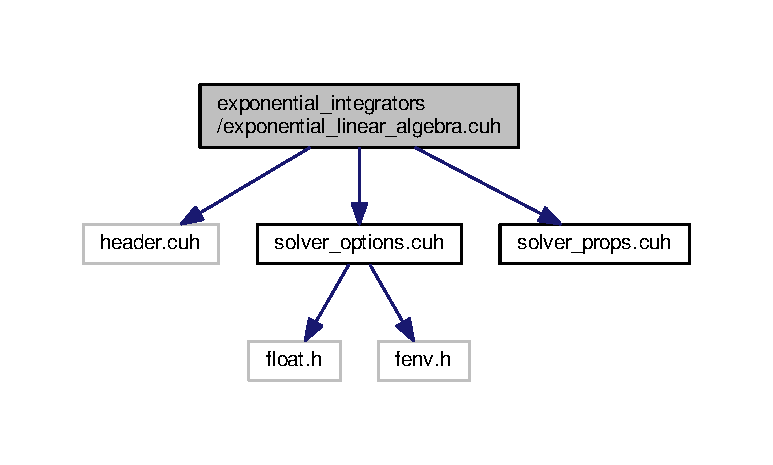
\includegraphics[width=350pt]{exponential__linear__algebra_8cuh__incl}
\end{center}
\end{figure}
This graph shows which files directly or indirectly include this file\+:\nopagebreak
\begin{figure}[H]
\begin{center}
\leavevmode
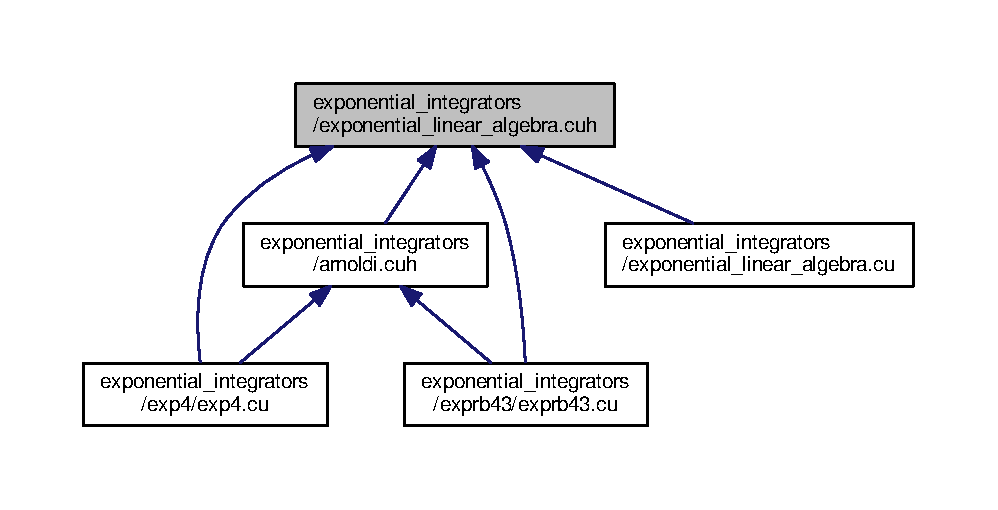
\includegraphics[width=350pt]{exponential__linear__algebra_8cuh__dep__incl}
\end{center}
\end{figure}
\subsection*{Macros}
\begin{DoxyCompactItemize}
\item 
\#define \hyperlink{exponential__linear__algebra_8cuh_a681edd700cfabbc96d9bafca7cc69049}{E\+X\+P\+O\+N\+E\+N\+T\+I\+A\+L\+\_\+\+L\+I\+N\+E\+A\+R\+\_\+\+A\+L\+G\+E\+B\+R\+A\+\_\+\+C\+UH}
\end{DoxyCompactItemize}
\subsection*{Functions}
\begin{DoxyCompactItemize}
\item 
\+\_\+\+\_\+device\+\_\+\+\_\+ void \hyperlink{exponential__linear__algebra_8cuh_a2e59348b99908b5918de88097e15d5ff}{matvec\+\_\+m\+\_\+by\+\_\+m} (const int m, const double $\ast$const \+\_\+\+\_\+restrict\+\_\+\+\_\+ A, const double $\ast$const \+\_\+\+\_\+restrict\+\_\+\+\_\+ V, double $\ast$const \+\_\+\+\_\+restrict\+\_\+\+\_\+ Av)
\begin{DoxyCompactList}\small\item\em Matrix-\/vector multiplication of a matrix sized MxM and a vector Mx1. \end{DoxyCompactList}\item 
\+\_\+\+\_\+device\+\_\+\+\_\+ void \hyperlink{exponential__linear__algebra_8cuh_a6bc7e5c08b8e40b19ce05ea146c05307}{matvec\+\_\+m\+\_\+by\+\_\+m\+\_\+plusequal} (const int m, const double $\ast$const \+\_\+\+\_\+restrict\+\_\+\+\_\+ A, const double $\ast$const \+\_\+\+\_\+restrict\+\_\+\+\_\+ V, double $\ast$const \+\_\+\+\_\+restrict\+\_\+\+\_\+ Av)
\begin{DoxyCompactList}\small\item\em Matrix-\/vector plus equals for a matrix of size MxM and vector of size Mx1. That is, it returns (A + I) $\ast$ v. \end{DoxyCompactList}\item 
\+\_\+\+\_\+device\+\_\+\+\_\+ void \hyperlink{exponential__linear__algebra_8cuh_a03e37312683db492dc73e08c17fe40e7}{matvec\+\_\+n\+\_\+by\+\_\+m\+\_\+scale} (const int m, const double \hyperlink{radau2a_8cu_a4fab5866449108992478041d2e51a28c}{scale}, const double $\ast$const \+\_\+\+\_\+restrict\+\_\+\+\_\+ A, const double $\ast$const \+\_\+\+\_\+restrict\+\_\+\+\_\+ V, double $\ast$const \+\_\+\+\_\+restrict\+\_\+\+\_\+ Av)
\begin{DoxyCompactList}\small\item\em Matrix-\/vector multiplication of a matrix sized N\+S\+PxM and a vector of size Mx1 scaled by a specified factor That is, it returns A $\ast$ v $\ast$ scale. \end{DoxyCompactList}\item 
\+\_\+\+\_\+device\+\_\+\+\_\+ void \hyperlink{exponential__linear__algebra_8cuh_aafe924c72a847b1d591e8fecb0efebdc}{matvec\+\_\+n\+\_\+by\+\_\+m\+\_\+scale\+\_\+special} (const int m, const double $\ast$\+\_\+\+\_\+restrict\+\_\+\+\_\+ \hyperlink{radau2a_8cu_a4fab5866449108992478041d2e51a28c}{scale}, const double $\ast$\+\_\+\+\_\+restrict\+\_\+\+\_\+ A, double $\ast$const \+\_\+\+\_\+restrict\+\_\+\+\_\+ $\ast$V, double $\ast$\+\_\+\+\_\+restrict\+\_\+\+\_\+ $\ast$Av)
\begin{DoxyCompactList}\small\item\em Matrix-\/vector multiplication of a matrix sized N\+S\+PxM and a vector of size Mx1 scaled by a specified factor. \end{DoxyCompactList}\item 
\+\_\+\+\_\+device\+\_\+\+\_\+ void \hyperlink{exponential__linear__algebra_8cuh_a6d511f330da8ea1a044ed327a132d290}{matvec\+\_\+n\+\_\+by\+\_\+m\+\_\+scale\+\_\+special2} (const int m, const double $\ast$\+\_\+\+\_\+restrict\+\_\+\+\_\+ \hyperlink{radau2a_8cu_a4fab5866449108992478041d2e51a28c}{scale}, const double $\ast$\+\_\+\+\_\+restrict\+\_\+\+\_\+ A, double $\ast$const \+\_\+\+\_\+restrict\+\_\+\+\_\+ $\ast$V, double $\ast$\+\_\+\+\_\+restrict\+\_\+\+\_\+ $\ast$Av)
\begin{DoxyCompactList}\small\item\em Matrix-\/vector multiplication of a matrix sized N\+S\+PxM and a vector of size Mx1 scaled by a specified factor. \end{DoxyCompactList}\item 
\+\_\+\+\_\+device\+\_\+\+\_\+ void \hyperlink{exponential__linear__algebra_8cuh_a28166d4c2569ab108219b8466bef8a77}{matvec\+\_\+n\+\_\+by\+\_\+m\+\_\+scale\+\_\+add} (const int m, const double \hyperlink{radau2a_8cu_a4fab5866449108992478041d2e51a28c}{scale}, const double $\ast$\+\_\+\+\_\+restrict\+\_\+\+\_\+ add, const double $\ast$\+\_\+\+\_\+restrict\+\_\+\+\_\+ A, double $\ast$\+\_\+\+\_\+restrict\+\_\+\+\_\+ V, const double $\ast$\+\_\+\+\_\+restrict\+\_\+\+\_\+ Av)
\begin{DoxyCompactList}\small\item\em Matrix-\/vector multiplication of a matrix sized N\+S\+PxM and a vector of size Mx1 scaled by a specified factor and added to another vector. \end{DoxyCompactList}\item 
\+\_\+\+\_\+device\+\_\+\+\_\+ void \hyperlink{exponential__linear__algebra_8cuh_a0522be133cda40ce325a2af6d95daddb}{matvec\+\_\+n\+\_\+by\+\_\+m\+\_\+scale\+\_\+add\+\_\+subtract} (const int m, const double \hyperlink{radau2a_8cu_a4fab5866449108992478041d2e51a28c}{scale}, const double $\ast$\+\_\+\+\_\+restrict\+\_\+\+\_\+ A, const double $\ast$V, double $\ast$\+\_\+\+\_\+restrict\+\_\+\+\_\+ Av, const double $\ast$\+\_\+\+\_\+restrict\+\_\+\+\_\+ add, const double $\ast$\+\_\+\+\_\+restrict\+\_\+\+\_\+ sub)
\begin{DoxyCompactList}\small\item\em Matrix-\/vector multiplication of a matrix sized N\+S\+PxM and a vector of size Mx1 scaled by a specified factor and adds and subtracts the specified vectors note, the addition is twice the specified vector. \end{DoxyCompactList}\item 
\+\_\+\+\_\+device\+\_\+\+\_\+ void \hyperlink{exponential__linear__algebra_8cuh_ace23ed149f65a9b90469b38ecd9ef01b}{scale} (const double $\ast$\+\_\+\+\_\+restrict\+\_\+\+\_\+ y0, const double $\ast$\+\_\+\+\_\+restrict\+\_\+\+\_\+ y1, double $\ast$\+\_\+\+\_\+restrict\+\_\+\+\_\+ sc)
\begin{DoxyCompactList}\small\item\em Get scaling for weighted norm. \end{DoxyCompactList}\item 
\+\_\+\+\_\+device\+\_\+\+\_\+ void \hyperlink{exponential__linear__algebra_8cuh_a2e7ea5b129b2e703fcc6aeb3affadd64}{scale\+\_\+init} (const double $\ast$\+\_\+\+\_\+restrict\+\_\+\+\_\+ y0, double $\ast$\+\_\+\+\_\+restrict\+\_\+\+\_\+ sc)
\begin{DoxyCompactList}\small\item\em Get scaling for weighted norm for the initial timestep (used in krylov process) \end{DoxyCompactList}\item 
\+\_\+\+\_\+device\+\_\+\+\_\+ double \hyperlink{exponential__linear__algebra_8cuh_a0c015672153032287ee1abbde6487d41}{sc\+\_\+norm} (const double $\ast$\+\_\+\+\_\+restrict\+\_\+\+\_\+ nums, const double $\ast$\+\_\+\+\_\+restrict\+\_\+\+\_\+ sc)
\begin{DoxyCompactList}\small\item\em Perform weighted norm. \end{DoxyCompactList}\item 
\+\_\+\+\_\+device\+\_\+\+\_\+ double \hyperlink{exponential__linear__algebra_8cuh_aa0074f06fcc396f12514f858ab825ca8}{two\+\_\+norm} (const double $\ast$\+\_\+\+\_\+restrict\+\_\+\+\_\+ v)
\begin{DoxyCompactList}\small\item\em Computes and returns the two norm of a vector. \end{DoxyCompactList}\item 
\+\_\+\+\_\+device\+\_\+\+\_\+ double \hyperlink{exponential__linear__algebra_8cuh_ae01ed1392756734c2d6996554cb20176}{normalize} (const double $\ast$\+\_\+\+\_\+restrict\+\_\+\+\_\+ v, double $\ast$\+\_\+\+\_\+restrict\+\_\+\+\_\+ v\+\_\+out)
\begin{DoxyCompactList}\small\item\em Normalize the input vector using a 2-\/norm. \end{DoxyCompactList}\item 
\+\_\+\+\_\+device\+\_\+\+\_\+ double \hyperlink{exponential__linear__algebra_8cuh_a43b8d535f44e58015de9b6ea37561bd7}{dotproduct} (const double $\ast$\+\_\+\+\_\+restrict\+\_\+\+\_\+ w, const double $\ast$\+\_\+\+\_\+restrict\+\_\+\+\_\+ Vm)
\begin{DoxyCompactList}\small\item\em Performs the dot product of the w (N\+SP x 1) vector with the given subspace vector (N\+SP x 1) \end{DoxyCompactList}\item 
\+\_\+\+\_\+device\+\_\+\+\_\+ void \hyperlink{exponential__linear__algebra_8cuh_a6b815eec17077505cb9313d6c380e036}{scale\+\_\+subtract} (const double s, const double $\ast$\+\_\+\+\_\+restrict\+\_\+\+\_\+ Vm, double $\ast$\+\_\+\+\_\+restrict\+\_\+\+\_\+ w)
\begin{DoxyCompactList}\small\item\em Subtracts Vm scaled by s from w. \end{DoxyCompactList}\item 
\+\_\+\+\_\+device\+\_\+\+\_\+ void \hyperlink{exponential__linear__algebra_8cuh_a5349e6f114398db5a19e212fc837f670}{scale\+\_\+mult} (const double s, const double $\ast$\+\_\+\+\_\+restrict\+\_\+\+\_\+ w, double $\ast$\+\_\+\+\_\+restrict\+\_\+\+\_\+ Vm)
\begin{DoxyCompactList}\small\item\em Sets Vm to s $\ast$ w. \end{DoxyCompactList}\end{DoxyCompactItemize}


\subsection{Macro Definition Documentation}
\index{exponential\+\_\+linear\+\_\+algebra.\+cuh@{exponential\+\_\+linear\+\_\+algebra.\+cuh}!E\+X\+P\+O\+N\+E\+N\+T\+I\+A\+L\+\_\+\+L\+I\+N\+E\+A\+R\+\_\+\+A\+L\+G\+E\+B\+R\+A\+\_\+\+C\+UH@{E\+X\+P\+O\+N\+E\+N\+T\+I\+A\+L\+\_\+\+L\+I\+N\+E\+A\+R\+\_\+\+A\+L\+G\+E\+B\+R\+A\+\_\+\+C\+UH}}
\index{E\+X\+P\+O\+N\+E\+N\+T\+I\+A\+L\+\_\+\+L\+I\+N\+E\+A\+R\+\_\+\+A\+L\+G\+E\+B\+R\+A\+\_\+\+C\+UH@{E\+X\+P\+O\+N\+E\+N\+T\+I\+A\+L\+\_\+\+L\+I\+N\+E\+A\+R\+\_\+\+A\+L\+G\+E\+B\+R\+A\+\_\+\+C\+UH}!exponential\+\_\+linear\+\_\+algebra.\+cuh@{exponential\+\_\+linear\+\_\+algebra.\+cuh}}
\subsubsection[{\texorpdfstring{E\+X\+P\+O\+N\+E\+N\+T\+I\+A\+L\+\_\+\+L\+I\+N\+E\+A\+R\+\_\+\+A\+L\+G\+E\+B\+R\+A\+\_\+\+C\+UH}{EXPONENTIAL_LINEAR_ALGEBRA_CUH}}]{\setlength{\rightskip}{0pt plus 5cm}\#define E\+X\+P\+O\+N\+E\+N\+T\+I\+A\+L\+\_\+\+L\+I\+N\+E\+A\+R\+\_\+\+A\+L\+G\+E\+B\+R\+A\+\_\+\+C\+UH}\hypertarget{exponential__linear__algebra_8cuh_a681edd700cfabbc96d9bafca7cc69049}{}\label{exponential__linear__algebra_8cuh_a681edd700cfabbc96d9bafca7cc69049}


\subsection{Function Documentation}
\index{exponential\+\_\+linear\+\_\+algebra.\+cuh@{exponential\+\_\+linear\+\_\+algebra.\+cuh}!dotproduct@{dotproduct}}
\index{dotproduct@{dotproduct}!exponential\+\_\+linear\+\_\+algebra.\+cuh@{exponential\+\_\+linear\+\_\+algebra.\+cuh}}
\subsubsection[{\texorpdfstring{dotproduct(const double $\ast$\+\_\+\+\_\+restrict\+\_\+\+\_\+ w, const double $\ast$\+\_\+\+\_\+restrict\+\_\+\+\_\+ Vm)}{dotproduct(const double *__restrict__ w, const double *__restrict__ Vm)}}]{\setlength{\rightskip}{0pt plus 5cm}\+\_\+\+\_\+device\+\_\+\+\_\+ double dotproduct (
\begin{DoxyParamCaption}
\item[{const double $\ast$\+\_\+\+\_\+restrict\+\_\+\+\_\+}]{w, }
\item[{const double $\ast$\+\_\+\+\_\+restrict\+\_\+\+\_\+}]{Vm}
\end{DoxyParamCaption}
)}\hypertarget{exponential__linear__algebra_8cuh_a43b8d535f44e58015de9b6ea37561bd7}{}\label{exponential__linear__algebra_8cuh_a43b8d535f44e58015de9b6ea37561bd7}


Performs the dot product of the w (N\+SP x 1) vector with the given subspace vector (N\+SP x 1) 

returns $Vm \dot w$


\begin{DoxyParams}[1]{Parameters}
\mbox{\tt in}  & {\em w} & the vector with with to dot \\
\hline
\mbox{\tt in}  & {\em Vm} & the subspace vector \\
\hline
\end{DoxyParams}
\begin{DoxyReturn}{Returns}
sum -\/ the dot product of the specified vectors 
\end{DoxyReturn}
\index{exponential\+\_\+linear\+\_\+algebra.\+cuh@{exponential\+\_\+linear\+\_\+algebra.\+cuh}!matvec\+\_\+m\+\_\+by\+\_\+m@{matvec\+\_\+m\+\_\+by\+\_\+m}}
\index{matvec\+\_\+m\+\_\+by\+\_\+m@{matvec\+\_\+m\+\_\+by\+\_\+m}!exponential\+\_\+linear\+\_\+algebra.\+cuh@{exponential\+\_\+linear\+\_\+algebra.\+cuh}}
\subsubsection[{\texorpdfstring{matvec\+\_\+m\+\_\+by\+\_\+m(const int m, const double $\ast$const \+\_\+\+\_\+restrict\+\_\+\+\_\+ A, const double $\ast$const \+\_\+\+\_\+restrict\+\_\+\+\_\+ V, double $\ast$const \+\_\+\+\_\+restrict\+\_\+\+\_\+ Av)}{matvec_m_by_m(const int m, const double *const __restrict__ A, const double *const __restrict__ V, double *const __restrict__ Av)}}]{\setlength{\rightskip}{0pt plus 5cm}\+\_\+\+\_\+device\+\_\+\+\_\+ void matvec\+\_\+m\+\_\+by\+\_\+m (
\begin{DoxyParamCaption}
\item[{const int}]{m, }
\item[{const double $\ast$const \+\_\+\+\_\+restrict\+\_\+\+\_\+}]{A, }
\item[{const double $\ast$const \+\_\+\+\_\+restrict\+\_\+\+\_\+}]{V, }
\item[{double $\ast$const \+\_\+\+\_\+restrict\+\_\+\+\_\+}]{Av}
\end{DoxyParamCaption}
)}\hypertarget{exponential__linear__algebra_8cuh_a2e59348b99908b5918de88097e15d5ff}{}\label{exponential__linear__algebra_8cuh_a2e59348b99908b5918de88097e15d5ff}


Matrix-\/vector multiplication of a matrix sized MxM and a vector Mx1. 


\begin{DoxyParams}[1]{Parameters}
\mbox{\tt in}  & {\em m} & size of the matrix \\
\hline
\mbox{\tt in}  & {\em A} & matrix of size MxM \\
\hline
\mbox{\tt in}  & {\em V} & vector of size Mx1 \\
\hline
\mbox{\tt out}  & {\em Av} & vector that is A $\ast$ v \\
\hline
\end{DoxyParams}
\index{exponential\+\_\+linear\+\_\+algebra.\+cuh@{exponential\+\_\+linear\+\_\+algebra.\+cuh}!matvec\+\_\+m\+\_\+by\+\_\+m\+\_\+plusequal@{matvec\+\_\+m\+\_\+by\+\_\+m\+\_\+plusequal}}
\index{matvec\+\_\+m\+\_\+by\+\_\+m\+\_\+plusequal@{matvec\+\_\+m\+\_\+by\+\_\+m\+\_\+plusequal}!exponential\+\_\+linear\+\_\+algebra.\+cuh@{exponential\+\_\+linear\+\_\+algebra.\+cuh}}
\subsubsection[{\texorpdfstring{matvec\+\_\+m\+\_\+by\+\_\+m\+\_\+plusequal(const int m, const double $\ast$const \+\_\+\+\_\+restrict\+\_\+\+\_\+ A, const double $\ast$const \+\_\+\+\_\+restrict\+\_\+\+\_\+ V, double $\ast$const \+\_\+\+\_\+restrict\+\_\+\+\_\+ Av)}{matvec_m_by_m_plusequal(const int m, const double *const __restrict__ A, const double *const __restrict__ V, double *const __restrict__ Av)}}]{\setlength{\rightskip}{0pt plus 5cm}\+\_\+\+\_\+device\+\_\+\+\_\+ void matvec\+\_\+m\+\_\+by\+\_\+m\+\_\+plusequal (
\begin{DoxyParamCaption}
\item[{const int}]{m, }
\item[{const double $\ast$const \+\_\+\+\_\+restrict\+\_\+\+\_\+}]{A, }
\item[{const double $\ast$const \+\_\+\+\_\+restrict\+\_\+\+\_\+}]{V, }
\item[{double $\ast$const \+\_\+\+\_\+restrict\+\_\+\+\_\+}]{Av}
\end{DoxyParamCaption}
)}\hypertarget{exponential__linear__algebra_8cuh_a6bc7e5c08b8e40b19ce05ea146c05307}{}\label{exponential__linear__algebra_8cuh_a6bc7e5c08b8e40b19ce05ea146c05307}


Matrix-\/vector plus equals for a matrix of size MxM and vector of size Mx1. That is, it returns (A + I) $\ast$ v. 


\begin{DoxyParams}[1]{Parameters}
\mbox{\tt in}  & {\em m} & size of the matrix \\
\hline
\mbox{\tt in}  & {\em A} & matrix of size MxM \\
\hline
\mbox{\tt in}  & {\em V} & vector of size Mx1 \\
\hline
\mbox{\tt out}  & {\em Av} & vector that is (A + I) $\ast$ v \\
\hline
\end{DoxyParams}
\index{exponential\+\_\+linear\+\_\+algebra.\+cuh@{exponential\+\_\+linear\+\_\+algebra.\+cuh}!matvec\+\_\+n\+\_\+by\+\_\+m\+\_\+scale@{matvec\+\_\+n\+\_\+by\+\_\+m\+\_\+scale}}
\index{matvec\+\_\+n\+\_\+by\+\_\+m\+\_\+scale@{matvec\+\_\+n\+\_\+by\+\_\+m\+\_\+scale}!exponential\+\_\+linear\+\_\+algebra.\+cuh@{exponential\+\_\+linear\+\_\+algebra.\+cuh}}
\subsubsection[{\texorpdfstring{matvec\+\_\+n\+\_\+by\+\_\+m\+\_\+scale(const int m, const double scale, const double $\ast$const \+\_\+\+\_\+restrict\+\_\+\+\_\+ A, const double $\ast$const \+\_\+\+\_\+restrict\+\_\+\+\_\+ V, double $\ast$const \+\_\+\+\_\+restrict\+\_\+\+\_\+ Av)}{matvec_n_by_m_scale(const int m, const double scale, const double *const __restrict__ A, const double *const __restrict__ V, double *const __restrict__ Av)}}]{\setlength{\rightskip}{0pt plus 5cm}\+\_\+\+\_\+device\+\_\+\+\_\+ void matvec\+\_\+n\+\_\+by\+\_\+m\+\_\+scale (
\begin{DoxyParamCaption}
\item[{const int}]{m, }
\item[{const double}]{scale, }
\item[{const double $\ast$const \+\_\+\+\_\+restrict\+\_\+\+\_\+}]{A, }
\item[{const double $\ast$const \+\_\+\+\_\+restrict\+\_\+\+\_\+}]{V, }
\item[{double $\ast$const \+\_\+\+\_\+restrict\+\_\+\+\_\+}]{Av}
\end{DoxyParamCaption}
)}\hypertarget{exponential__linear__algebra_8cuh_a03e37312683db492dc73e08c17fe40e7}{}\label{exponential__linear__algebra_8cuh_a03e37312683db492dc73e08c17fe40e7}


Matrix-\/vector multiplication of a matrix sized N\+S\+PxM and a vector of size Mx1 scaled by a specified factor That is, it returns A $\ast$ v $\ast$ scale. 


\begin{DoxyParams}[1]{Parameters}
\mbox{\tt in}  & {\em m} & size of the matrix \\
\hline
\mbox{\tt in}  & {\em scale} & a number to scale the multplication by \\
\hline
\mbox{\tt in}  & {\em A} & matrix \\
\hline
\mbox{\tt in}  & {\em V} & the vector \\
\hline
\mbox{\tt out}  & {\em Av} & vector that is A $\ast$ V $\ast$ scale \\
\hline
\end{DoxyParams}
\index{exponential\+\_\+linear\+\_\+algebra.\+cuh@{exponential\+\_\+linear\+\_\+algebra.\+cuh}!matvec\+\_\+n\+\_\+by\+\_\+m\+\_\+scale\+\_\+add@{matvec\+\_\+n\+\_\+by\+\_\+m\+\_\+scale\+\_\+add}}
\index{matvec\+\_\+n\+\_\+by\+\_\+m\+\_\+scale\+\_\+add@{matvec\+\_\+n\+\_\+by\+\_\+m\+\_\+scale\+\_\+add}!exponential\+\_\+linear\+\_\+algebra.\+cuh@{exponential\+\_\+linear\+\_\+algebra.\+cuh}}
\subsubsection[{\texorpdfstring{matvec\+\_\+n\+\_\+by\+\_\+m\+\_\+scale\+\_\+add(const int m, const double scale, const double $\ast$\+\_\+\+\_\+restrict\+\_\+\+\_\+ add, const double $\ast$\+\_\+\+\_\+restrict\+\_\+\+\_\+ A, double $\ast$\+\_\+\+\_\+restrict\+\_\+\+\_\+ V, const double $\ast$\+\_\+\+\_\+restrict\+\_\+\+\_\+ Av)}{matvec_n_by_m_scale_add(const int m, const double scale, const double *__restrict__ add, const double *__restrict__ A, double *__restrict__ V, const double *__restrict__ Av)}}]{\setlength{\rightskip}{0pt plus 5cm}\+\_\+\+\_\+device\+\_\+\+\_\+ void matvec\+\_\+n\+\_\+by\+\_\+m\+\_\+scale\+\_\+add (
\begin{DoxyParamCaption}
\item[{const int}]{m, }
\item[{const double}]{scale, }
\item[{const double $\ast$\+\_\+\+\_\+restrict\+\_\+\+\_\+}]{add, }
\item[{const double $\ast$\+\_\+\+\_\+restrict\+\_\+\+\_\+}]{A, }
\item[{double $\ast$\+\_\+\+\_\+restrict\+\_\+\+\_\+}]{V, }
\item[{const double $\ast$\+\_\+\+\_\+restrict\+\_\+\+\_\+}]{Av}
\end{DoxyParamCaption}
)}\hypertarget{exponential__linear__algebra_8cuh_a28166d4c2569ab108219b8466bef8a77}{}\label{exponential__linear__algebra_8cuh_a28166d4c2569ab108219b8466bef8a77}


Matrix-\/vector multiplication of a matrix sized N\+S\+PxM and a vector of size Mx1 scaled by a specified factor and added to another vector. 

Computes $A * V * scale + add$


\begin{DoxyParams}[1]{Parameters}
\mbox{\tt in}  & {\em m} & size of the matrix \\
\hline
\mbox{\tt in}  & {\em scale} & a number to scale the multplication by \\
\hline
\mbox{\tt in}  & {\em add} & the vector to add to the result \\
\hline
\mbox{\tt in}  & {\em A} & matrix \\
\hline
\mbox{\tt in}  & {\em V} & the vector \\
\hline
\mbox{\tt out}  & {\em Av} & vector that is A $\ast$ V $\ast$ scale + add \\
\hline
\end{DoxyParams}
\index{exponential\+\_\+linear\+\_\+algebra.\+cuh@{exponential\+\_\+linear\+\_\+algebra.\+cuh}!matvec\+\_\+n\+\_\+by\+\_\+m\+\_\+scale\+\_\+add\+\_\+subtract@{matvec\+\_\+n\+\_\+by\+\_\+m\+\_\+scale\+\_\+add\+\_\+subtract}}
\index{matvec\+\_\+n\+\_\+by\+\_\+m\+\_\+scale\+\_\+add\+\_\+subtract@{matvec\+\_\+n\+\_\+by\+\_\+m\+\_\+scale\+\_\+add\+\_\+subtract}!exponential\+\_\+linear\+\_\+algebra.\+cuh@{exponential\+\_\+linear\+\_\+algebra.\+cuh}}
\subsubsection[{\texorpdfstring{matvec\+\_\+n\+\_\+by\+\_\+m\+\_\+scale\+\_\+add\+\_\+subtract(const int m, const double scale, const double $\ast$\+\_\+\+\_\+restrict\+\_\+\+\_\+ A, const double $\ast$\+V, double $\ast$\+\_\+\+\_\+restrict\+\_\+\+\_\+ Av, const double $\ast$\+\_\+\+\_\+restrict\+\_\+\+\_\+ add, const double $\ast$\+\_\+\+\_\+restrict\+\_\+\+\_\+ sub)}{matvec_n_by_m_scale_add_subtract(const int m, const double scale, const double *__restrict__ A, const double *V, double *__restrict__ Av, const double *__restrict__ add, const double *__restrict__ sub)}}]{\setlength{\rightskip}{0pt plus 5cm}\+\_\+\+\_\+device\+\_\+\+\_\+ void matvec\+\_\+n\+\_\+by\+\_\+m\+\_\+scale\+\_\+add\+\_\+subtract (
\begin{DoxyParamCaption}
\item[{const int}]{m, }
\item[{const double}]{scale, }
\item[{const double $\ast$\+\_\+\+\_\+restrict\+\_\+\+\_\+}]{A, }
\item[{const double $\ast$}]{V, }
\item[{double $\ast$\+\_\+\+\_\+restrict\+\_\+\+\_\+}]{Av, }
\item[{const double $\ast$\+\_\+\+\_\+restrict\+\_\+\+\_\+}]{add, }
\item[{const double $\ast$\+\_\+\+\_\+restrict\+\_\+\+\_\+}]{sub}
\end{DoxyParamCaption}
)}\hypertarget{exponential__linear__algebra_8cuh_a0522be133cda40ce325a2af6d95daddb}{}\label{exponential__linear__algebra_8cuh_a0522be133cda40ce325a2af6d95daddb}


Matrix-\/vector multiplication of a matrix sized N\+S\+PxM and a vector of size Mx1 scaled by a specified factor and adds and subtracts the specified vectors note, the addition is twice the specified vector. 

Computes $scale * A * V + 2 * add - sub$


\begin{DoxyParams}[1]{Parameters}
\mbox{\tt in}  & {\em m} & size of the matrix \\
\hline
\mbox{\tt in}  & {\em scale} & a number to scale the multplication by \\
\hline
\mbox{\tt in}  & {\em A} & matrix \\
\hline
\mbox{\tt in}  & {\em V} & the vector \\
\hline
\mbox{\tt out}  & {\em Av} & vector that is scale $\ast$ A $\ast$ V + 2 $\ast$ add -\/ sub \\
\hline
\mbox{\tt in}  & {\em add} & the vector to add to the result \\
\hline
\mbox{\tt in}  & {\em sub} & the vector to subtract from the result \\
\hline
\end{DoxyParams}
\index{exponential\+\_\+linear\+\_\+algebra.\+cuh@{exponential\+\_\+linear\+\_\+algebra.\+cuh}!matvec\+\_\+n\+\_\+by\+\_\+m\+\_\+scale\+\_\+special@{matvec\+\_\+n\+\_\+by\+\_\+m\+\_\+scale\+\_\+special}}
\index{matvec\+\_\+n\+\_\+by\+\_\+m\+\_\+scale\+\_\+special@{matvec\+\_\+n\+\_\+by\+\_\+m\+\_\+scale\+\_\+special}!exponential\+\_\+linear\+\_\+algebra.\+cuh@{exponential\+\_\+linear\+\_\+algebra.\+cuh}}
\subsubsection[{\texorpdfstring{matvec\+\_\+n\+\_\+by\+\_\+m\+\_\+scale\+\_\+special(const int m, const double $\ast$\+\_\+\+\_\+restrict\+\_\+\+\_\+ scale, const double $\ast$\+\_\+\+\_\+restrict\+\_\+\+\_\+ A, double $\ast$const \+\_\+\+\_\+restrict\+\_\+\+\_\+ $\ast$\+V, double $\ast$\+\_\+\+\_\+restrict\+\_\+\+\_\+ $\ast$\+Av)}{matvec_n_by_m_scale_special(const int m, const double *__restrict__ scale, const double *__restrict__ A, double *const __restrict__ *V, double *__restrict__ *Av)}}]{\setlength{\rightskip}{0pt plus 5cm}\+\_\+\+\_\+device\+\_\+\+\_\+ void matvec\+\_\+n\+\_\+by\+\_\+m\+\_\+scale\+\_\+special (
\begin{DoxyParamCaption}
\item[{const int}]{m, }
\item[{const double $\ast$\+\_\+\+\_\+restrict\+\_\+\+\_\+}]{scale, }
\item[{const double $\ast$\+\_\+\+\_\+restrict\+\_\+\+\_\+}]{A, }
\item[{double $\ast$const \+\_\+\+\_\+restrict\+\_\+\+\_\+ $\ast$}]{V, }
\item[{double $\ast$\+\_\+\+\_\+restrict\+\_\+\+\_\+ $\ast$}]{Av}
\end{DoxyParamCaption}
)}\hypertarget{exponential__linear__algebra_8cuh_aafe924c72a847b1d591e8fecb0efebdc}{}\label{exponential__linear__algebra_8cuh_aafe924c72a847b1d591e8fecb0efebdc}


Matrix-\/vector multiplication of a matrix sized N\+S\+PxM and a vector of size Mx1 scaled by a specified factor. 

Computes the following\+: $Av1 = A * V1 * scale[0]$, $Av2 = A * V2 * scale[1]$, and $Av3 = A * V3 * scale[2] + V4 + V5$


\begin{DoxyParams}[1]{Parameters}
\mbox{\tt in}  & {\em m} & size of the matrix \\
\hline
\mbox{\tt in}  & {\em scale} & a list of numbers to scale the multplication by \\
\hline
\mbox{\tt in}  & {\em A} & matrix \\
\hline
\mbox{\tt in}  & {\em V} & a list of 5 pointers corresponding to V1, V2, V3, V4, V5 \\
\hline
\mbox{\tt out}  & {\em Av} & a list of 3 pointers corresponding to Av1, Av2, Av3 \\
\hline
\end{DoxyParams}
\index{exponential\+\_\+linear\+\_\+algebra.\+cuh@{exponential\+\_\+linear\+\_\+algebra.\+cuh}!matvec\+\_\+n\+\_\+by\+\_\+m\+\_\+scale\+\_\+special2@{matvec\+\_\+n\+\_\+by\+\_\+m\+\_\+scale\+\_\+special2}}
\index{matvec\+\_\+n\+\_\+by\+\_\+m\+\_\+scale\+\_\+special2@{matvec\+\_\+n\+\_\+by\+\_\+m\+\_\+scale\+\_\+special2}!exponential\+\_\+linear\+\_\+algebra.\+cuh@{exponential\+\_\+linear\+\_\+algebra.\+cuh}}
\subsubsection[{\texorpdfstring{matvec\+\_\+n\+\_\+by\+\_\+m\+\_\+scale\+\_\+special2(const int m, const double $\ast$\+\_\+\+\_\+restrict\+\_\+\+\_\+ scale, const double $\ast$\+\_\+\+\_\+restrict\+\_\+\+\_\+ A, double $\ast$const \+\_\+\+\_\+restrict\+\_\+\+\_\+ $\ast$\+V, double $\ast$\+\_\+\+\_\+restrict\+\_\+\+\_\+ $\ast$\+Av)}{matvec_n_by_m_scale_special2(const int m, const double *__restrict__ scale, const double *__restrict__ A, double *const __restrict__ *V, double *__restrict__ *Av)}}]{\setlength{\rightskip}{0pt plus 5cm}\+\_\+\+\_\+device\+\_\+\+\_\+ void matvec\+\_\+n\+\_\+by\+\_\+m\+\_\+scale\+\_\+special2 (
\begin{DoxyParamCaption}
\item[{const int}]{m, }
\item[{const double $\ast$\+\_\+\+\_\+restrict\+\_\+\+\_\+}]{scale, }
\item[{const double $\ast$\+\_\+\+\_\+restrict\+\_\+\+\_\+}]{A, }
\item[{double $\ast$const \+\_\+\+\_\+restrict\+\_\+\+\_\+ $\ast$}]{V, }
\item[{double $\ast$\+\_\+\+\_\+restrict\+\_\+\+\_\+ $\ast$}]{Av}
\end{DoxyParamCaption}
)}\hypertarget{exponential__linear__algebra_8cuh_a6d511f330da8ea1a044ed327a132d290}{}\label{exponential__linear__algebra_8cuh_a6d511f330da8ea1a044ed327a132d290}


Matrix-\/vector multiplication of a matrix sized N\+S\+PxM and a vector of size Mx1 scaled by a specified factor. 

Computes the following\+: $Av1 = A * V1 * scale[0]$ and\+: $Av2 = A * V2 * scale[1]$

Performs inline matrix-\/vector multiplication (with unrolled loops)


\begin{DoxyParams}[1]{Parameters}
\mbox{\tt in}  & {\em m} & size of the matrix \\
\hline
\mbox{\tt in}  & {\em scale} & a list of numbers to scale the multplication by \\
\hline
\mbox{\tt in}  & {\em A} & matrix \\
\hline
\mbox{\tt in}  & {\em V} & a list of 2 pointers corresponding to V1, V2 \\
\hline
\mbox{\tt out}  & {\em Av} & a list of 2 pointers corresponding to Av1, Av2 \\
\hline
\end{DoxyParams}
\index{exponential\+\_\+linear\+\_\+algebra.\+cuh@{exponential\+\_\+linear\+\_\+algebra.\+cuh}!normalize@{normalize}}
\index{normalize@{normalize}!exponential\+\_\+linear\+\_\+algebra.\+cuh@{exponential\+\_\+linear\+\_\+algebra.\+cuh}}
\subsubsection[{\texorpdfstring{normalize(const double $\ast$\+\_\+\+\_\+restrict\+\_\+\+\_\+ v, double $\ast$\+\_\+\+\_\+restrict\+\_\+\+\_\+ v\+\_\+out)}{normalize(const double *__restrict__ v, double *__restrict__ v_out)}}]{\setlength{\rightskip}{0pt plus 5cm}\+\_\+\+\_\+device\+\_\+\+\_\+ double normalize (
\begin{DoxyParamCaption}
\item[{const double $\ast$\+\_\+\+\_\+restrict\+\_\+\+\_\+}]{v, }
\item[{double $\ast$\+\_\+\+\_\+restrict\+\_\+\+\_\+}]{v\+\_\+out}
\end{DoxyParamCaption}
)}\hypertarget{exponential__linear__algebra_8cuh_ae01ed1392756734c2d6996554cb20176}{}\label{exponential__linear__algebra_8cuh_ae01ed1392756734c2d6996554cb20176}


Normalize the input vector using a 2-\/norm. 

$v_{out} = \frac{v}{\left| v \right|}_2$


\begin{DoxyParams}[1]{Parameters}
\mbox{\tt in}  & {\em v} & vector to be normalized \\
\hline
\mbox{\tt out}  & {\em v\+\_\+out} & where to stick the normalized part of v (in a column) \\
\hline
\end{DoxyParams}
\index{exponential\+\_\+linear\+\_\+algebra.\+cuh@{exponential\+\_\+linear\+\_\+algebra.\+cuh}!sc\+\_\+norm@{sc\+\_\+norm}}
\index{sc\+\_\+norm@{sc\+\_\+norm}!exponential\+\_\+linear\+\_\+algebra.\+cuh@{exponential\+\_\+linear\+\_\+algebra.\+cuh}}
\subsubsection[{\texorpdfstring{sc\+\_\+norm(const double $\ast$\+\_\+\+\_\+restrict\+\_\+\+\_\+ nums, const double $\ast$\+\_\+\+\_\+restrict\+\_\+\+\_\+ sc)}{sc_norm(const double *__restrict__ nums, const double *__restrict__ sc)}}]{\setlength{\rightskip}{0pt plus 5cm}\+\_\+\+\_\+device\+\_\+\+\_\+ double sc\+\_\+norm (
\begin{DoxyParamCaption}
\item[{const double $\ast$\+\_\+\+\_\+restrict\+\_\+\+\_\+}]{nums, }
\item[{const double $\ast$\+\_\+\+\_\+restrict\+\_\+\+\_\+}]{sc}
\end{DoxyParamCaption}
)}\hypertarget{exponential__linear__algebra_8cuh_a0c015672153032287ee1abbde6487d41}{}\label{exponential__linear__algebra_8cuh_a0c015672153032287ee1abbde6487d41}


Perform weighted norm. 

Computes $\left| nums * sc\right|_2$


\begin{DoxyParams}[1]{Parameters}
\mbox{\tt in}  & {\em nums} & values to be normed \\
\hline
\mbox{\tt in}  & {\em sc} & scaling array for norm \\
\hline
\end{DoxyParams}
\begin{DoxyReturn}{Returns}
norm weighted norm 
\end{DoxyReturn}
\index{exponential\+\_\+linear\+\_\+algebra.\+cuh@{exponential\+\_\+linear\+\_\+algebra.\+cuh}!scale@{scale}}
\index{scale@{scale}!exponential\+\_\+linear\+\_\+algebra.\+cuh@{exponential\+\_\+linear\+\_\+algebra.\+cuh}}
\subsubsection[{\texorpdfstring{scale(const double $\ast$\+\_\+\+\_\+restrict\+\_\+\+\_\+ y0, const double $\ast$\+\_\+\+\_\+restrict\+\_\+\+\_\+ y1, double $\ast$\+\_\+\+\_\+restrict\+\_\+\+\_\+ sc)}{scale(const double *__restrict__ y0, const double *__restrict__ y1, double *__restrict__ sc)}}]{\setlength{\rightskip}{0pt plus 5cm}\+\_\+\+\_\+device\+\_\+\+\_\+ void scale (
\begin{DoxyParamCaption}
\item[{const double $\ast$\+\_\+\+\_\+restrict\+\_\+\+\_\+}]{y0, }
\item[{const double $\ast$\+\_\+\+\_\+restrict\+\_\+\+\_\+}]{y1, }
\item[{double $\ast$\+\_\+\+\_\+restrict\+\_\+\+\_\+}]{sc}
\end{DoxyParamCaption}
)}\hypertarget{exponential__linear__algebra_8cuh_ace23ed149f65a9b90469b38ecd9ef01b}{}\label{exponential__linear__algebra_8cuh_ace23ed149f65a9b90469b38ecd9ef01b}


Get scaling for weighted norm. 

Computes $\frac{1.0}{ATOL + \max\left(\left|y0\right|, \left|y1\right|) * RTOL\right)}$


\begin{DoxyParams}[1]{Parameters}
\mbox{\tt in}  & {\em y0} & values at current timestep \\
\hline
\mbox{\tt in}  & {\em y1} & values at next timestep \\
\hline
\mbox{\tt out}  & {\em sc} & array of scaling values \\
\hline
\end{DoxyParams}
\index{exponential\+\_\+linear\+\_\+algebra.\+cuh@{exponential\+\_\+linear\+\_\+algebra.\+cuh}!scale\+\_\+init@{scale\+\_\+init}}
\index{scale\+\_\+init@{scale\+\_\+init}!exponential\+\_\+linear\+\_\+algebra.\+cuh@{exponential\+\_\+linear\+\_\+algebra.\+cuh}}
\subsubsection[{\texorpdfstring{scale\+\_\+init(const double $\ast$\+\_\+\+\_\+restrict\+\_\+\+\_\+ y0, double $\ast$\+\_\+\+\_\+restrict\+\_\+\+\_\+ sc)}{scale_init(const double *__restrict__ y0, double *__restrict__ sc)}}]{\setlength{\rightskip}{0pt plus 5cm}\+\_\+\+\_\+device\+\_\+\+\_\+ void scale\+\_\+init (
\begin{DoxyParamCaption}
\item[{const double $\ast$\+\_\+\+\_\+restrict\+\_\+\+\_\+}]{y0, }
\item[{double $\ast$\+\_\+\+\_\+restrict\+\_\+\+\_\+}]{sc}
\end{DoxyParamCaption}
)}\hypertarget{exponential__linear__algebra_8cuh_a2e7ea5b129b2e703fcc6aeb3affadd64}{}\label{exponential__linear__algebra_8cuh_a2e7ea5b129b2e703fcc6aeb3affadd64}


Get scaling for weighted norm for the initial timestep (used in krylov process) 


\begin{DoxyParams}[1]{Parameters}
\mbox{\tt in}  & {\em y0} & values at current timestep \\
\hline
\mbox{\tt out}  & {\em sc} & array of scaling values \\
\hline
\end{DoxyParams}
\index{exponential\+\_\+linear\+\_\+algebra.\+cuh@{exponential\+\_\+linear\+\_\+algebra.\+cuh}!scale\+\_\+mult@{scale\+\_\+mult}}
\index{scale\+\_\+mult@{scale\+\_\+mult}!exponential\+\_\+linear\+\_\+algebra.\+cuh@{exponential\+\_\+linear\+\_\+algebra.\+cuh}}
\subsubsection[{\texorpdfstring{scale\+\_\+mult(const double s, const double $\ast$\+\_\+\+\_\+restrict\+\_\+\+\_\+ w, double $\ast$\+\_\+\+\_\+restrict\+\_\+\+\_\+ Vm)}{scale_mult(const double s, const double *__restrict__ w, double *__restrict__ Vm)}}]{\setlength{\rightskip}{0pt plus 5cm}\+\_\+\+\_\+device\+\_\+\+\_\+ void scale\+\_\+mult (
\begin{DoxyParamCaption}
\item[{const double}]{s, }
\item[{const double $\ast$\+\_\+\+\_\+restrict\+\_\+\+\_\+}]{w, }
\item[{double $\ast$\+\_\+\+\_\+restrict\+\_\+\+\_\+}]{Vm}
\end{DoxyParamCaption}
)}\hypertarget{exponential__linear__algebra_8cuh_a5349e6f114398db5a19e212fc837f670}{}\label{exponential__linear__algebra_8cuh_a5349e6f114398db5a19e212fc837f670}


Sets Vm to s $\ast$ w. 

$Vm = s * w$


\begin{DoxyParams}[1]{Parameters}
\mbox{\tt in}  & {\em s} & the scale multiplier to use \\
\hline
\mbox{\tt in}  & {\em w} & the vector to use as a base \\
\hline
\mbox{\tt out}  & {\em Vm} & the subspace matrix to set \\
\hline
\end{DoxyParams}
\index{exponential\+\_\+linear\+\_\+algebra.\+cuh@{exponential\+\_\+linear\+\_\+algebra.\+cuh}!scale\+\_\+subtract@{scale\+\_\+subtract}}
\index{scale\+\_\+subtract@{scale\+\_\+subtract}!exponential\+\_\+linear\+\_\+algebra.\+cuh@{exponential\+\_\+linear\+\_\+algebra.\+cuh}}
\subsubsection[{\texorpdfstring{scale\+\_\+subtract(const double s, const double $\ast$\+\_\+\+\_\+restrict\+\_\+\+\_\+ Vm, double $\ast$\+\_\+\+\_\+restrict\+\_\+\+\_\+ w)}{scale_subtract(const double s, const double *__restrict__ Vm, double *__restrict__ w)}}]{\setlength{\rightskip}{0pt plus 5cm}\+\_\+\+\_\+device\+\_\+\+\_\+ void scale\+\_\+subtract (
\begin{DoxyParamCaption}
\item[{const double}]{s, }
\item[{const double $\ast$\+\_\+\+\_\+restrict\+\_\+\+\_\+}]{Vm, }
\item[{double $\ast$\+\_\+\+\_\+restrict\+\_\+\+\_\+}]{w}
\end{DoxyParamCaption}
)}\hypertarget{exponential__linear__algebra_8cuh_a6b815eec17077505cb9313d6c380e036}{}\label{exponential__linear__algebra_8cuh_a6b815eec17077505cb9313d6c380e036}


Subtracts Vm scaled by s from w. 

$ w -= Vm * s$


\begin{DoxyParams}[1]{Parameters}
\mbox{\tt in}  & {\em s} & the scale multiplier to use \\
\hline
\mbox{\tt in}  & {\em Vm} & the subspace matrix \\
\hline
\mbox{\tt out}  & {\em w} & the vector to subtract from \\
\hline
\end{DoxyParams}
\index{exponential\+\_\+linear\+\_\+algebra.\+cuh@{exponential\+\_\+linear\+\_\+algebra.\+cuh}!two\+\_\+norm@{two\+\_\+norm}}
\index{two\+\_\+norm@{two\+\_\+norm}!exponential\+\_\+linear\+\_\+algebra.\+cuh@{exponential\+\_\+linear\+\_\+algebra.\+cuh}}
\subsubsection[{\texorpdfstring{two\+\_\+norm(const double $\ast$\+\_\+\+\_\+restrict\+\_\+\+\_\+ v)}{two_norm(const double *__restrict__ v)}}]{\setlength{\rightskip}{0pt plus 5cm}\+\_\+\+\_\+device\+\_\+\+\_\+ double two\+\_\+norm (
\begin{DoxyParamCaption}
\item[{const double $\ast$\+\_\+\+\_\+restrict\+\_\+\+\_\+}]{v}
\end{DoxyParamCaption}
)}\hypertarget{exponential__linear__algebra_8cuh_aa0074f06fcc396f12514f858ab825ca8}{}\label{exponential__linear__algebra_8cuh_aa0074f06fcc396f12514f858ab825ca8}


Computes and returns the two norm of a vector. 

Computes $\sqrt{\sum{v^2}}$


\begin{DoxyParams}[1]{Parameters}
\mbox{\tt in}  & {\em v} & the vector \\
\hline
\end{DoxyParams}

\hypertarget{exponential__linear__algebra_8h}{}\section{exponential\+\_\+integrators/exponential\+\_\+linear\+\_\+algebra.h File Reference}
\label{exponential__linear__algebra_8h}\index{exponential\+\_\+integrators/exponential\+\_\+linear\+\_\+algebra.\+h@{exponential\+\_\+integrators/exponential\+\_\+linear\+\_\+algebra.\+h}}


Implementation of various linear algebra functions needed in the exponential integrators.  


{\ttfamily \#include \char`\"{}header.\+h\char`\"{}}\\*
{\ttfamily \#include \char`\"{}solver\+\_\+options.\+h\char`\"{}}\\*
{\ttfamily \#include \char`\"{}solver\+\_\+props.\+h\char`\"{}}\\*
Include dependency graph for exponential\+\_\+linear\+\_\+algebra.\+h\+:\nopagebreak
\begin{figure}[H]
\begin{center}
\leavevmode
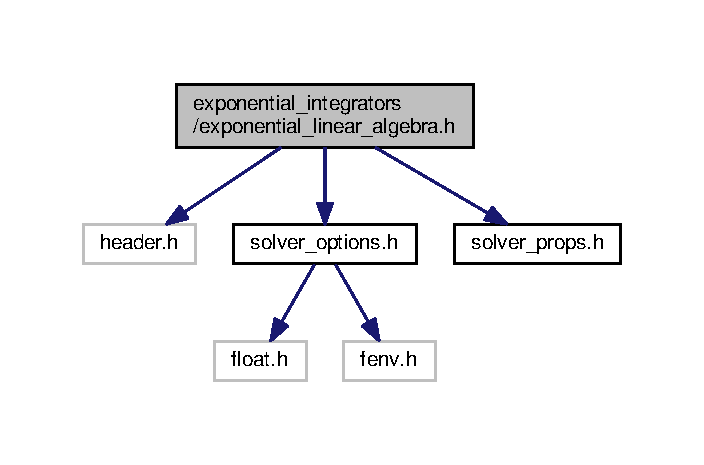
\includegraphics[width=338pt]{exponential__linear__algebra_8h__incl}
\end{center}
\end{figure}
This graph shows which files directly or indirectly include this file\+:\nopagebreak
\begin{figure}[H]
\begin{center}
\leavevmode
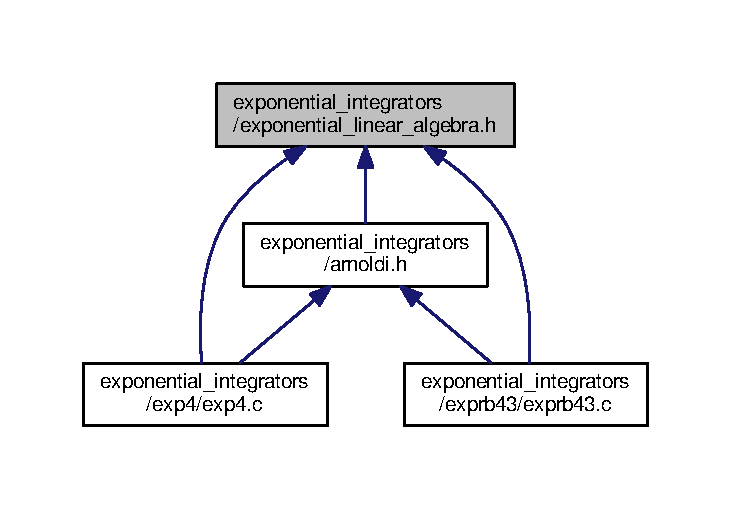
\includegraphics[width=350pt]{exponential__linear__algebra_8h__dep__incl}
\end{center}
\end{figure}
\subsection*{Functions}
\begin{DoxyCompactItemize}
\item 
static void \hyperlink{exponential__linear__algebra_8h_acafa9c4220de7efc4de6a5ed8c3e1967}{matvec\+\_\+m\+\_\+by\+\_\+m} (const int m, const double $\ast$\+\_\+\+\_\+restrict\+\_\+\+\_\+ A, const double $\ast$\+\_\+\+\_\+restrict\+\_\+\+\_\+ V, double $\ast$\+\_\+\+\_\+restrict\+\_\+\+\_\+ Av)
\begin{DoxyCompactList}\small\item\em Matrix-\/vector multiplication of a matrix sized MxM and a vector Mx1. \end{DoxyCompactList}\item 
static void \hyperlink{exponential__linear__algebra_8h_ab027a8e5ad8aea990d03ae7a6a4241e7}{matvec\+\_\+m\+\_\+by\+\_\+m\+\_\+plusequal} (const int m, const double $\ast$\+\_\+\+\_\+restrict\+\_\+\+\_\+ A, const double $\ast$\+\_\+\+\_\+restrict\+\_\+\+\_\+ V, double $\ast$\+\_\+\+\_\+restrict\+\_\+\+\_\+ Av)
\begin{DoxyCompactList}\small\item\em Matrix-\/vector plus equals for a matrix of size MxM and vector of size Mx1. That is, it returns (A + I) $\ast$ v. \end{DoxyCompactList}\item 
static void \hyperlink{exponential__linear__algebra_8h_ade2d6860c24502d2946d9cbfa8f95e33}{matvec\+\_\+n\+\_\+by\+\_\+m\+\_\+scale} (const int m, const double \hyperlink{radau2a_8cu_a4fab5866449108992478041d2e51a28c}{scale}, const double $\ast$\+\_\+\+\_\+restrict\+\_\+\+\_\+ A, const double $\ast$\+\_\+\+\_\+restrict\+\_\+\+\_\+ V, double $\ast$\+\_\+\+\_\+restrict\+\_\+\+\_\+ Av)
\begin{DoxyCompactList}\small\item\em Matrix-\/vector multiplication of a matrix sized N\+S\+PxM and a vector of size Mx1 scaled by a specified factor That is, it returns A $\ast$ v $\ast$ scale. \end{DoxyCompactList}\item 
static void \hyperlink{exponential__linear__algebra_8h_a890e0818ff5e99c5987afba1fa4b4191}{matvec\+\_\+n\+\_\+by\+\_\+m\+\_\+scale\+\_\+special} (const int m, const double $\ast$\+\_\+\+\_\+restrict\+\_\+\+\_\+ \hyperlink{radau2a_8cu_a4fab5866449108992478041d2e51a28c}{scale}, const double $\ast$\+\_\+\+\_\+restrict\+\_\+\+\_\+ A, const double $\ast$$\ast$\+\_\+\+\_\+restrict\+\_\+\+\_\+ V, double $\ast$$\ast$\+\_\+\+\_\+restrict\+\_\+\+\_\+ Av)
\begin{DoxyCompactList}\small\item\em Matrix-\/vector multiplication of a matrix sized N\+S\+PxM and a vector of size Mx1 scaled by a specified factor. \end{DoxyCompactList}\item 
static void \hyperlink{exponential__linear__algebra_8h_a352714cca74d693b14d0f6f7d0487343}{matvec\+\_\+n\+\_\+by\+\_\+m\+\_\+scale\+\_\+special2} (const int m, const double $\ast$\+\_\+\+\_\+restrict\+\_\+\+\_\+ \hyperlink{radau2a_8cu_a4fab5866449108992478041d2e51a28c}{scale}, const double $\ast$\+\_\+\+\_\+restrict\+\_\+\+\_\+ A, const double $\ast$$\ast$\+\_\+\+\_\+restrict\+\_\+\+\_\+ V, double $\ast$$\ast$\+\_\+\+\_\+restrict\+\_\+\+\_\+ Av)
\begin{DoxyCompactList}\small\item\em Matrix-\/vector multiplication of a matrix sized N\+S\+PxM and a vector of size Mx1 scaled by a specified factor. \end{DoxyCompactList}\item 
static void \hyperlink{exponential__linear__algebra_8h_a97605c6ef788b1454da1fb480c8f60d7}{matvec\+\_\+n\+\_\+by\+\_\+m\+\_\+scale\+\_\+add} (const int m, const double \hyperlink{radau2a_8cu_a4fab5866449108992478041d2e51a28c}{scale}, const double $\ast$\+\_\+\+\_\+restrict\+\_\+\+\_\+ A, const double $\ast$\+\_\+\+\_\+restrict\+\_\+\+\_\+ V, double $\ast$\+\_\+\+\_\+restrict\+\_\+\+\_\+ Av, const double $\ast$\+\_\+\+\_\+restrict\+\_\+\+\_\+ add)
\begin{DoxyCompactList}\small\item\em Matrix-\/vector multiplication of a matrix sized N\+S\+PxM and a vector of size Mx1 scaled by a specified factor and added to another vector. \end{DoxyCompactList}\item 
static void \hyperlink{exponential__linear__algebra_8h_a59b6cf94f2d125f0442a275da26e411e}{matvec\+\_\+n\+\_\+by\+\_\+m\+\_\+scale\+\_\+add\+\_\+subtract} (const int m, const double \hyperlink{radau2a_8cu_a4fab5866449108992478041d2e51a28c}{scale}, const double $\ast$\+\_\+\+\_\+restrict\+\_\+\+\_\+ A, const double $\ast$\+\_\+\+\_\+restrict\+\_\+\+\_\+ V, double $\ast$\+\_\+\+\_\+restrict\+\_\+\+\_\+ Av, const double $\ast$\+\_\+\+\_\+restrict\+\_\+\+\_\+ add, const double $\ast$\+\_\+\+\_\+restrict\+\_\+\+\_\+ sub)
\begin{DoxyCompactList}\small\item\em Matrix-\/vector multiplication of a matrix sized N\+S\+PxM and a vector of size Mx1 scaled by a specified factor and adds and subtracts the specified vectors note, the addition is twice the specified vector. \end{DoxyCompactList}\item 
static void \hyperlink{exponential__linear__algebra_8h_ab98c11f729f92214cbc1a89f27949ec6}{scale} (const double $\ast$\+\_\+\+\_\+restrict\+\_\+\+\_\+ y0, const double $\ast$\+\_\+\+\_\+restrict\+\_\+\+\_\+ y1, double $\ast$\+\_\+\+\_\+restrict\+\_\+\+\_\+ sc)
\begin{DoxyCompactList}\small\item\em Get scaling for weighted norm. \end{DoxyCompactList}\item 
static void \hyperlink{exponential__linear__algebra_8h_a6eedf6c4f32ef93c4fa7f3ed6ed42224}{scale\+\_\+init} (const double $\ast$\+\_\+\+\_\+restrict\+\_\+\+\_\+ y0, double $\ast$\+\_\+\+\_\+restrict\+\_\+\+\_\+ sc)
\begin{DoxyCompactList}\small\item\em Get scaling for weighted norm for the initial timestep (used in krylov process) \end{DoxyCompactList}\item 
static double \hyperlink{exponential__linear__algebra_8h_adf3387803c6dc14a5e1f93870b61a875}{sc\+\_\+norm} (const double $\ast$\+\_\+\+\_\+restrict\+\_\+\+\_\+ nums, const double $\ast$\+\_\+\+\_\+restrict\+\_\+\+\_\+ sc)
\begin{DoxyCompactList}\small\item\em Perform weighted norm. \end{DoxyCompactList}\item 
static double \hyperlink{exponential__linear__algebra_8h_a2d10f1fcdc2240cb1d18dad7583479e9}{two\+\_\+norm} (const double $\ast$\+\_\+\+\_\+restrict\+\_\+\+\_\+ v)
\begin{DoxyCompactList}\small\item\em Computes and returns the two norm of a vector. \end{DoxyCompactList}\item 
static double \hyperlink{exponential__linear__algebra_8h_ad032c6988b7c57956f3d6d44957ac241}{normalize} (const double $\ast$\+\_\+\+\_\+restrict\+\_\+\+\_\+ v, double $\ast$\+\_\+\+\_\+restrict\+\_\+\+\_\+ v\+\_\+out)
\begin{DoxyCompactList}\small\item\em Normalize the input vector using a 2-\/norm. \end{DoxyCompactList}\item 
static double \hyperlink{exponential__linear__algebra_8h_afe704435bfc4dde0c5115869dea30907}{dotproduct} (const double $\ast$\+\_\+\+\_\+restrict\+\_\+\+\_\+ w, const double $\ast$\+\_\+\+\_\+restrict\+\_\+\+\_\+ Vm)
\begin{DoxyCompactList}\small\item\em Performs the dot product of the w (N\+SP x 1) vector with the given subspace vector (N\+SP x 1) \end{DoxyCompactList}\item 
static void \hyperlink{exponential__linear__algebra_8h_aef2d9e0d5a40be3499caadf4e94a3dfc}{scale\+\_\+subtract} (const double s, const double $\ast$\+\_\+\+\_\+restrict\+\_\+\+\_\+ Vm, double $\ast$\+\_\+\+\_\+restrict\+\_\+\+\_\+ w)
\begin{DoxyCompactList}\small\item\em Subtracts Vm scaled by s from w. \end{DoxyCompactList}\item 
static void \hyperlink{exponential__linear__algebra_8h_a4794916f728186d70fde648e381e32c0}{scale\+\_\+mult} (const double s, const double $\ast$\+\_\+\+\_\+restrict\+\_\+\+\_\+ w, double $\ast$\+\_\+\+\_\+restrict\+\_\+\+\_\+ Vm)
\begin{DoxyCompactList}\small\item\em Sets Vm to s $\ast$ w. \end{DoxyCompactList}\end{DoxyCompactItemize}


\subsection{Detailed Description}
Implementation of various linear algebra functions needed in the exponential integrators. 

\begin{DoxyAuthor}{Author}
Nicholas Curtis 
\end{DoxyAuthor}
\begin{DoxyDate}{Date}
03/09/2015 
\end{DoxyDate}


\subsection{Function Documentation}
\index{exponential\+\_\+linear\+\_\+algebra.\+h@{exponential\+\_\+linear\+\_\+algebra.\+h}!dotproduct@{dotproduct}}
\index{dotproduct@{dotproduct}!exponential\+\_\+linear\+\_\+algebra.\+h@{exponential\+\_\+linear\+\_\+algebra.\+h}}
\subsubsection[{\texorpdfstring{dotproduct(const double $\ast$\+\_\+\+\_\+restrict\+\_\+\+\_\+ w, const double $\ast$\+\_\+\+\_\+restrict\+\_\+\+\_\+ Vm)}{dotproduct(const double *__restrict__ w, const double *__restrict__ Vm)}}]{\setlength{\rightskip}{0pt plus 5cm}static double dotproduct (
\begin{DoxyParamCaption}
\item[{const double $\ast$\+\_\+\+\_\+restrict\+\_\+\+\_\+}]{w, }
\item[{const double $\ast$\+\_\+\+\_\+restrict\+\_\+\+\_\+}]{Vm}
\end{DoxyParamCaption}
)\hspace{0.3cm}{\ttfamily [inline]}, {\ttfamily [static]}}\hypertarget{exponential__linear__algebra_8h_afe704435bfc4dde0c5115869dea30907}{}\label{exponential__linear__algebra_8h_afe704435bfc4dde0c5115869dea30907}


Performs the dot product of the w (N\+SP x 1) vector with the given subspace vector (N\+SP x 1) 

returns $Vm \dot w$


\begin{DoxyParams}[1]{Parameters}
\mbox{\tt in}  & {\em w} & the vector with with to dot \\
\hline
\mbox{\tt in}  & {\em Vm} & the subspace vector \\
\hline
\end{DoxyParams}
\begin{DoxyReturn}{Returns}
sum -\/ the dot product of the specified vectors 
\end{DoxyReturn}
\index{exponential\+\_\+linear\+\_\+algebra.\+h@{exponential\+\_\+linear\+\_\+algebra.\+h}!matvec\+\_\+m\+\_\+by\+\_\+m@{matvec\+\_\+m\+\_\+by\+\_\+m}}
\index{matvec\+\_\+m\+\_\+by\+\_\+m@{matvec\+\_\+m\+\_\+by\+\_\+m}!exponential\+\_\+linear\+\_\+algebra.\+h@{exponential\+\_\+linear\+\_\+algebra.\+h}}
\subsubsection[{\texorpdfstring{matvec\+\_\+m\+\_\+by\+\_\+m(const int m, const double $\ast$\+\_\+\+\_\+restrict\+\_\+\+\_\+ A, const double $\ast$\+\_\+\+\_\+restrict\+\_\+\+\_\+ V, double $\ast$\+\_\+\+\_\+restrict\+\_\+\+\_\+ Av)}{matvec_m_by_m(const int m, const double *__restrict__ A, const double *__restrict__ V, double *__restrict__ Av)}}]{\setlength{\rightskip}{0pt plus 5cm}static void matvec\+\_\+m\+\_\+by\+\_\+m (
\begin{DoxyParamCaption}
\item[{const int}]{m, }
\item[{const double $\ast$\+\_\+\+\_\+restrict\+\_\+\+\_\+}]{A, }
\item[{const double $\ast$\+\_\+\+\_\+restrict\+\_\+\+\_\+}]{V, }
\item[{double $\ast$\+\_\+\+\_\+restrict\+\_\+\+\_\+}]{Av}
\end{DoxyParamCaption}
)\hspace{0.3cm}{\ttfamily [inline]}, {\ttfamily [static]}}\hypertarget{exponential__linear__algebra_8h_acafa9c4220de7efc4de6a5ed8c3e1967}{}\label{exponential__linear__algebra_8h_acafa9c4220de7efc4de6a5ed8c3e1967}


Matrix-\/vector multiplication of a matrix sized MxM and a vector Mx1. 


\begin{DoxyParams}[1]{Parameters}
\mbox{\tt in}  & {\em m} & size of the matrix \\
\hline
\mbox{\tt in}  & {\em A} & matrix of size MxM \\
\hline
\mbox{\tt in}  & {\em V} & vector of size Mx1 \\
\hline
\mbox{\tt out}  & {\em Av} & vector that is A $\ast$ v \\
\hline
\end{DoxyParams}
\index{exponential\+\_\+linear\+\_\+algebra.\+h@{exponential\+\_\+linear\+\_\+algebra.\+h}!matvec\+\_\+m\+\_\+by\+\_\+m\+\_\+plusequal@{matvec\+\_\+m\+\_\+by\+\_\+m\+\_\+plusequal}}
\index{matvec\+\_\+m\+\_\+by\+\_\+m\+\_\+plusequal@{matvec\+\_\+m\+\_\+by\+\_\+m\+\_\+plusequal}!exponential\+\_\+linear\+\_\+algebra.\+h@{exponential\+\_\+linear\+\_\+algebra.\+h}}
\subsubsection[{\texorpdfstring{matvec\+\_\+m\+\_\+by\+\_\+m\+\_\+plusequal(const int m, const double $\ast$\+\_\+\+\_\+restrict\+\_\+\+\_\+ A, const double $\ast$\+\_\+\+\_\+restrict\+\_\+\+\_\+ V, double $\ast$\+\_\+\+\_\+restrict\+\_\+\+\_\+ Av)}{matvec_m_by_m_plusequal(const int m, const double *__restrict__ A, const double *__restrict__ V, double *__restrict__ Av)}}]{\setlength{\rightskip}{0pt plus 5cm}static void matvec\+\_\+m\+\_\+by\+\_\+m\+\_\+plusequal (
\begin{DoxyParamCaption}
\item[{const int}]{m, }
\item[{const double $\ast$\+\_\+\+\_\+restrict\+\_\+\+\_\+}]{A, }
\item[{const double $\ast$\+\_\+\+\_\+restrict\+\_\+\+\_\+}]{V, }
\item[{double $\ast$\+\_\+\+\_\+restrict\+\_\+\+\_\+}]{Av}
\end{DoxyParamCaption}
)\hspace{0.3cm}{\ttfamily [inline]}, {\ttfamily [static]}}\hypertarget{exponential__linear__algebra_8h_ab027a8e5ad8aea990d03ae7a6a4241e7}{}\label{exponential__linear__algebra_8h_ab027a8e5ad8aea990d03ae7a6a4241e7}


Matrix-\/vector plus equals for a matrix of size MxM and vector of size Mx1. That is, it returns (A + I) $\ast$ v. 


\begin{DoxyParams}[1]{Parameters}
\mbox{\tt in}  & {\em m} & size of the matrix \\
\hline
\mbox{\tt in}  & {\em A} & matrix of size MxM \\
\hline
\mbox{\tt in}  & {\em V} & vector of size Mx1 \\
\hline
\mbox{\tt out}  & {\em Av} & vector that is (A + I) $\ast$ v \\
\hline
\end{DoxyParams}
\index{exponential\+\_\+linear\+\_\+algebra.\+h@{exponential\+\_\+linear\+\_\+algebra.\+h}!matvec\+\_\+n\+\_\+by\+\_\+m\+\_\+scale@{matvec\+\_\+n\+\_\+by\+\_\+m\+\_\+scale}}
\index{matvec\+\_\+n\+\_\+by\+\_\+m\+\_\+scale@{matvec\+\_\+n\+\_\+by\+\_\+m\+\_\+scale}!exponential\+\_\+linear\+\_\+algebra.\+h@{exponential\+\_\+linear\+\_\+algebra.\+h}}
\subsubsection[{\texorpdfstring{matvec\+\_\+n\+\_\+by\+\_\+m\+\_\+scale(const int m, const double scale, const double $\ast$\+\_\+\+\_\+restrict\+\_\+\+\_\+ A, const double $\ast$\+\_\+\+\_\+restrict\+\_\+\+\_\+ V, double $\ast$\+\_\+\+\_\+restrict\+\_\+\+\_\+ Av)}{matvec_n_by_m_scale(const int m, const double scale, const double *__restrict__ A, const double *__restrict__ V, double *__restrict__ Av)}}]{\setlength{\rightskip}{0pt plus 5cm}static void matvec\+\_\+n\+\_\+by\+\_\+m\+\_\+scale (
\begin{DoxyParamCaption}
\item[{const int}]{m, }
\item[{const double}]{scale, }
\item[{const double $\ast$\+\_\+\+\_\+restrict\+\_\+\+\_\+}]{A, }
\item[{const double $\ast$\+\_\+\+\_\+restrict\+\_\+\+\_\+}]{V, }
\item[{double $\ast$\+\_\+\+\_\+restrict\+\_\+\+\_\+}]{Av}
\end{DoxyParamCaption}
)\hspace{0.3cm}{\ttfamily [inline]}, {\ttfamily [static]}}\hypertarget{exponential__linear__algebra_8h_ade2d6860c24502d2946d9cbfa8f95e33}{}\label{exponential__linear__algebra_8h_ade2d6860c24502d2946d9cbfa8f95e33}


Matrix-\/vector multiplication of a matrix sized N\+S\+PxM and a vector of size Mx1 scaled by a specified factor That is, it returns A $\ast$ v $\ast$ scale. 


\begin{DoxyParams}[1]{Parameters}
\mbox{\tt in}  & {\em m} & size of the matrix \\
\hline
\mbox{\tt in}  & {\em scale} & a number to scale the multplication by \\
\hline
\mbox{\tt in}  & {\em A} & matrix \\
\hline
\mbox{\tt in}  & {\em V} & the vector \\
\hline
\mbox{\tt out}  & {\em Av} & vector that is A $\ast$ V $\ast$ scale \\
\hline
\end{DoxyParams}
\index{exponential\+\_\+linear\+\_\+algebra.\+h@{exponential\+\_\+linear\+\_\+algebra.\+h}!matvec\+\_\+n\+\_\+by\+\_\+m\+\_\+scale\+\_\+add@{matvec\+\_\+n\+\_\+by\+\_\+m\+\_\+scale\+\_\+add}}
\index{matvec\+\_\+n\+\_\+by\+\_\+m\+\_\+scale\+\_\+add@{matvec\+\_\+n\+\_\+by\+\_\+m\+\_\+scale\+\_\+add}!exponential\+\_\+linear\+\_\+algebra.\+h@{exponential\+\_\+linear\+\_\+algebra.\+h}}
\subsubsection[{\texorpdfstring{matvec\+\_\+n\+\_\+by\+\_\+m\+\_\+scale\+\_\+add(const int m, const double scale, const double $\ast$\+\_\+\+\_\+restrict\+\_\+\+\_\+ A, const double $\ast$\+\_\+\+\_\+restrict\+\_\+\+\_\+ V, double $\ast$\+\_\+\+\_\+restrict\+\_\+\+\_\+ Av, const double $\ast$\+\_\+\+\_\+restrict\+\_\+\+\_\+ add)}{matvec_n_by_m_scale_add(const int m, const double scale, const double *__restrict__ A, const double *__restrict__ V, double *__restrict__ Av, const double *__restrict__ add)}}]{\setlength{\rightskip}{0pt plus 5cm}static void matvec\+\_\+n\+\_\+by\+\_\+m\+\_\+scale\+\_\+add (
\begin{DoxyParamCaption}
\item[{const int}]{m, }
\item[{const double}]{scale, }
\item[{const double $\ast$\+\_\+\+\_\+restrict\+\_\+\+\_\+}]{A, }
\item[{const double $\ast$\+\_\+\+\_\+restrict\+\_\+\+\_\+}]{V, }
\item[{double $\ast$\+\_\+\+\_\+restrict\+\_\+\+\_\+}]{Av, }
\item[{const double $\ast$\+\_\+\+\_\+restrict\+\_\+\+\_\+}]{add}
\end{DoxyParamCaption}
)\hspace{0.3cm}{\ttfamily [inline]}, {\ttfamily [static]}}\hypertarget{exponential__linear__algebra_8h_a97605c6ef788b1454da1fb480c8f60d7}{}\label{exponential__linear__algebra_8h_a97605c6ef788b1454da1fb480c8f60d7}


Matrix-\/vector multiplication of a matrix sized N\+S\+PxM and a vector of size Mx1 scaled by a specified factor and added to another vector. 

Computes $A * V * scale + add$


\begin{DoxyParams}[1]{Parameters}
\mbox{\tt in}  & {\em m} & size of the matrix \\
\hline
\mbox{\tt in}  & {\em scale} & a number to scale the multplication by \\
\hline
\mbox{\tt in}  & {\em add} & the vector to add to the result \\
\hline
\mbox{\tt in}  & {\em A} & matrix \\
\hline
\mbox{\tt in}  & {\em V} & the vector \\
\hline
\mbox{\tt out}  & {\em Av} & vector that is A $\ast$ V $\ast$ scale + add \\
\hline
\end{DoxyParams}
\index{exponential\+\_\+linear\+\_\+algebra.\+h@{exponential\+\_\+linear\+\_\+algebra.\+h}!matvec\+\_\+n\+\_\+by\+\_\+m\+\_\+scale\+\_\+add\+\_\+subtract@{matvec\+\_\+n\+\_\+by\+\_\+m\+\_\+scale\+\_\+add\+\_\+subtract}}
\index{matvec\+\_\+n\+\_\+by\+\_\+m\+\_\+scale\+\_\+add\+\_\+subtract@{matvec\+\_\+n\+\_\+by\+\_\+m\+\_\+scale\+\_\+add\+\_\+subtract}!exponential\+\_\+linear\+\_\+algebra.\+h@{exponential\+\_\+linear\+\_\+algebra.\+h}}
\subsubsection[{\texorpdfstring{matvec\+\_\+n\+\_\+by\+\_\+m\+\_\+scale\+\_\+add\+\_\+subtract(const int m, const double scale, const double $\ast$\+\_\+\+\_\+restrict\+\_\+\+\_\+ A, const double $\ast$\+\_\+\+\_\+restrict\+\_\+\+\_\+ V, double $\ast$\+\_\+\+\_\+restrict\+\_\+\+\_\+ Av, const double $\ast$\+\_\+\+\_\+restrict\+\_\+\+\_\+ add, const double $\ast$\+\_\+\+\_\+restrict\+\_\+\+\_\+ sub)}{matvec_n_by_m_scale_add_subtract(const int m, const double scale, const double *__restrict__ A, const double *__restrict__ V, double *__restrict__ Av, const double *__restrict__ add, const double *__restrict__ sub)}}]{\setlength{\rightskip}{0pt plus 5cm}static void matvec\+\_\+n\+\_\+by\+\_\+m\+\_\+scale\+\_\+add\+\_\+subtract (
\begin{DoxyParamCaption}
\item[{const int}]{m, }
\item[{const double}]{scale, }
\item[{const double $\ast$\+\_\+\+\_\+restrict\+\_\+\+\_\+}]{A, }
\item[{const double $\ast$\+\_\+\+\_\+restrict\+\_\+\+\_\+}]{V, }
\item[{double $\ast$\+\_\+\+\_\+restrict\+\_\+\+\_\+}]{Av, }
\item[{const double $\ast$\+\_\+\+\_\+restrict\+\_\+\+\_\+}]{add, }
\item[{const double $\ast$\+\_\+\+\_\+restrict\+\_\+\+\_\+}]{sub}
\end{DoxyParamCaption}
)\hspace{0.3cm}{\ttfamily [inline]}, {\ttfamily [static]}}\hypertarget{exponential__linear__algebra_8h_a59b6cf94f2d125f0442a275da26e411e}{}\label{exponential__linear__algebra_8h_a59b6cf94f2d125f0442a275da26e411e}


Matrix-\/vector multiplication of a matrix sized N\+S\+PxM and a vector of size Mx1 scaled by a specified factor and adds and subtracts the specified vectors note, the addition is twice the specified vector. 

Computes $scale * A * V + 2 * add - sub$


\begin{DoxyParams}[1]{Parameters}
\mbox{\tt in}  & {\em m} & size of the matrix \\
\hline
\mbox{\tt in}  & {\em scale} & a number to scale the multplication by \\
\hline
\mbox{\tt in}  & {\em A} & matrix \\
\hline
\mbox{\tt in}  & {\em V} & the vector \\
\hline
\mbox{\tt out}  & {\em Av} & vector that is scale $\ast$ A $\ast$ V + 2 $\ast$ add -\/ sub \\
\hline
\mbox{\tt in}  & {\em add} & the vector to add to the result \\
\hline
\mbox{\tt in}  & {\em sub} & the vector to subtract from the result \\
\hline
\end{DoxyParams}
\index{exponential\+\_\+linear\+\_\+algebra.\+h@{exponential\+\_\+linear\+\_\+algebra.\+h}!matvec\+\_\+n\+\_\+by\+\_\+m\+\_\+scale\+\_\+special@{matvec\+\_\+n\+\_\+by\+\_\+m\+\_\+scale\+\_\+special}}
\index{matvec\+\_\+n\+\_\+by\+\_\+m\+\_\+scale\+\_\+special@{matvec\+\_\+n\+\_\+by\+\_\+m\+\_\+scale\+\_\+special}!exponential\+\_\+linear\+\_\+algebra.\+h@{exponential\+\_\+linear\+\_\+algebra.\+h}}
\subsubsection[{\texorpdfstring{matvec\+\_\+n\+\_\+by\+\_\+m\+\_\+scale\+\_\+special(const int m, const double $\ast$\+\_\+\+\_\+restrict\+\_\+\+\_\+ scale, const double $\ast$\+\_\+\+\_\+restrict\+\_\+\+\_\+ A, const double $\ast$$\ast$\+\_\+\+\_\+restrict\+\_\+\+\_\+ V, double $\ast$$\ast$\+\_\+\+\_\+restrict\+\_\+\+\_\+ Av)}{matvec_n_by_m_scale_special(const int m, const double *__restrict__ scale, const double *__restrict__ A, const double **__restrict__ V, double **__restrict__ Av)}}]{\setlength{\rightskip}{0pt plus 5cm}static void matvec\+\_\+n\+\_\+by\+\_\+m\+\_\+scale\+\_\+special (
\begin{DoxyParamCaption}
\item[{const int}]{m, }
\item[{const double $\ast$\+\_\+\+\_\+restrict\+\_\+\+\_\+}]{scale, }
\item[{const double $\ast$\+\_\+\+\_\+restrict\+\_\+\+\_\+}]{A, }
\item[{const double $\ast$$\ast$\+\_\+\+\_\+restrict\+\_\+\+\_\+}]{V, }
\item[{double $\ast$$\ast$\+\_\+\+\_\+restrict\+\_\+\+\_\+}]{Av}
\end{DoxyParamCaption}
)\hspace{0.3cm}{\ttfamily [inline]}, {\ttfamily [static]}}\hypertarget{exponential__linear__algebra_8h_a890e0818ff5e99c5987afba1fa4b4191}{}\label{exponential__linear__algebra_8h_a890e0818ff5e99c5987afba1fa4b4191}


Matrix-\/vector multiplication of a matrix sized N\+S\+PxM and a vector of size Mx1 scaled by a specified factor. 

Computes the following\+: $Av1 = A * V1 * scale[0]$, $Av2 = A * V2 * scale[1]$, and $Av3 = A * V3 * scale[2] + V4 + V5$


\begin{DoxyParams}[1]{Parameters}
\mbox{\tt in}  & {\em m} & size of the matrix \\
\hline
\mbox{\tt in}  & {\em scale} & a list of numbers to scale the multplication by \\
\hline
\mbox{\tt in}  & {\em A} & matrix \\
\hline
\mbox{\tt in}  & {\em V} & a list of 5 pointers corresponding to V1, V2, V3, V4, V5 \\
\hline
\mbox{\tt out}  & {\em Av} & a list of 3 pointers corresponding to Av1, Av2, Av3 \\
\hline
\end{DoxyParams}
\index{exponential\+\_\+linear\+\_\+algebra.\+h@{exponential\+\_\+linear\+\_\+algebra.\+h}!matvec\+\_\+n\+\_\+by\+\_\+m\+\_\+scale\+\_\+special2@{matvec\+\_\+n\+\_\+by\+\_\+m\+\_\+scale\+\_\+special2}}
\index{matvec\+\_\+n\+\_\+by\+\_\+m\+\_\+scale\+\_\+special2@{matvec\+\_\+n\+\_\+by\+\_\+m\+\_\+scale\+\_\+special2}!exponential\+\_\+linear\+\_\+algebra.\+h@{exponential\+\_\+linear\+\_\+algebra.\+h}}
\subsubsection[{\texorpdfstring{matvec\+\_\+n\+\_\+by\+\_\+m\+\_\+scale\+\_\+special2(const int m, const double $\ast$\+\_\+\+\_\+restrict\+\_\+\+\_\+ scale, const double $\ast$\+\_\+\+\_\+restrict\+\_\+\+\_\+ A, const double $\ast$$\ast$\+\_\+\+\_\+restrict\+\_\+\+\_\+ V, double $\ast$$\ast$\+\_\+\+\_\+restrict\+\_\+\+\_\+ Av)}{matvec_n_by_m_scale_special2(const int m, const double *__restrict__ scale, const double *__restrict__ A, const double **__restrict__ V, double **__restrict__ Av)}}]{\setlength{\rightskip}{0pt plus 5cm}static void matvec\+\_\+n\+\_\+by\+\_\+m\+\_\+scale\+\_\+special2 (
\begin{DoxyParamCaption}
\item[{const int}]{m, }
\item[{const double $\ast$\+\_\+\+\_\+restrict\+\_\+\+\_\+}]{scale, }
\item[{const double $\ast$\+\_\+\+\_\+restrict\+\_\+\+\_\+}]{A, }
\item[{const double $\ast$$\ast$\+\_\+\+\_\+restrict\+\_\+\+\_\+}]{V, }
\item[{double $\ast$$\ast$\+\_\+\+\_\+restrict\+\_\+\+\_\+}]{Av}
\end{DoxyParamCaption}
)\hspace{0.3cm}{\ttfamily [inline]}, {\ttfamily [static]}}\hypertarget{exponential__linear__algebra_8h_a352714cca74d693b14d0f6f7d0487343}{}\label{exponential__linear__algebra_8h_a352714cca74d693b14d0f6f7d0487343}


Matrix-\/vector multiplication of a matrix sized N\+S\+PxM and a vector of size Mx1 scaled by a specified factor. 

Computes the following\+: $Av1 = A * V1 * scale[0]$ and\+: $Av2 = A * V2 * scale[1]$

Performs inline matrix-\/vector multiplication (with unrolled loops)


\begin{DoxyParams}[1]{Parameters}
\mbox{\tt in}  & {\em m} & size of the matrix \\
\hline
\mbox{\tt in}  & {\em scale} & a list of numbers to scale the multplication by \\
\hline
\mbox{\tt in}  & {\em A} & matrix \\
\hline
\mbox{\tt in}  & {\em V} & a list of 2 pointers corresponding to V1, V2 \\
\hline
\mbox{\tt out}  & {\em Av} & a list of 2 pointers corresponding to Av1, Av2 \\
\hline
\end{DoxyParams}
\index{exponential\+\_\+linear\+\_\+algebra.\+h@{exponential\+\_\+linear\+\_\+algebra.\+h}!normalize@{normalize}}
\index{normalize@{normalize}!exponential\+\_\+linear\+\_\+algebra.\+h@{exponential\+\_\+linear\+\_\+algebra.\+h}}
\subsubsection[{\texorpdfstring{normalize(const double $\ast$\+\_\+\+\_\+restrict\+\_\+\+\_\+ v, double $\ast$\+\_\+\+\_\+restrict\+\_\+\+\_\+ v\+\_\+out)}{normalize(const double *__restrict__ v, double *__restrict__ v_out)}}]{\setlength{\rightskip}{0pt plus 5cm}static double normalize (
\begin{DoxyParamCaption}
\item[{const double $\ast$\+\_\+\+\_\+restrict\+\_\+\+\_\+}]{v, }
\item[{double $\ast$\+\_\+\+\_\+restrict\+\_\+\+\_\+}]{v\+\_\+out}
\end{DoxyParamCaption}
)\hspace{0.3cm}{\ttfamily [inline]}, {\ttfamily [static]}}\hypertarget{exponential__linear__algebra_8h_ad032c6988b7c57956f3d6d44957ac241}{}\label{exponential__linear__algebra_8h_ad032c6988b7c57956f3d6d44957ac241}


Normalize the input vector using a 2-\/norm. 

$v_{out} = \frac{v}{\left| v \right|}_2$


\begin{DoxyParams}[1]{Parameters}
\mbox{\tt in}  & {\em v} & vector to be normalized \\
\hline
\mbox{\tt out}  & {\em v\+\_\+out} & where to stick the normalized part of v (in a column) \\
\hline
\end{DoxyParams}
\index{exponential\+\_\+linear\+\_\+algebra.\+h@{exponential\+\_\+linear\+\_\+algebra.\+h}!sc\+\_\+norm@{sc\+\_\+norm}}
\index{sc\+\_\+norm@{sc\+\_\+norm}!exponential\+\_\+linear\+\_\+algebra.\+h@{exponential\+\_\+linear\+\_\+algebra.\+h}}
\subsubsection[{\texorpdfstring{sc\+\_\+norm(const double $\ast$\+\_\+\+\_\+restrict\+\_\+\+\_\+ nums, const double $\ast$\+\_\+\+\_\+restrict\+\_\+\+\_\+ sc)}{sc_norm(const double *__restrict__ nums, const double *__restrict__ sc)}}]{\setlength{\rightskip}{0pt plus 5cm}static double sc\+\_\+norm (
\begin{DoxyParamCaption}
\item[{const double $\ast$\+\_\+\+\_\+restrict\+\_\+\+\_\+}]{nums, }
\item[{const double $\ast$\+\_\+\+\_\+restrict\+\_\+\+\_\+}]{sc}
\end{DoxyParamCaption}
)\hspace{0.3cm}{\ttfamily [inline]}, {\ttfamily [static]}}\hypertarget{exponential__linear__algebra_8h_adf3387803c6dc14a5e1f93870b61a875}{}\label{exponential__linear__algebra_8h_adf3387803c6dc14a5e1f93870b61a875}


Perform weighted norm. 

Computes $\left| nums * sc\right|_2$


\begin{DoxyParams}[1]{Parameters}
\mbox{\tt in}  & {\em nums} & values to be normed \\
\hline
\mbox{\tt in}  & {\em sc} & scaling array for norm \\
\hline
\end{DoxyParams}
\begin{DoxyReturn}{Returns}
norm weighted norm 
\end{DoxyReturn}
\index{exponential\+\_\+linear\+\_\+algebra.\+h@{exponential\+\_\+linear\+\_\+algebra.\+h}!scale@{scale}}
\index{scale@{scale}!exponential\+\_\+linear\+\_\+algebra.\+h@{exponential\+\_\+linear\+\_\+algebra.\+h}}
\subsubsection[{\texorpdfstring{scale(const double $\ast$\+\_\+\+\_\+restrict\+\_\+\+\_\+ y0, const double $\ast$\+\_\+\+\_\+restrict\+\_\+\+\_\+ y1, double $\ast$\+\_\+\+\_\+restrict\+\_\+\+\_\+ sc)}{scale(const double *__restrict__ y0, const double *__restrict__ y1, double *__restrict__ sc)}}]{\setlength{\rightskip}{0pt plus 5cm}static void scale (
\begin{DoxyParamCaption}
\item[{const double $\ast$\+\_\+\+\_\+restrict\+\_\+\+\_\+}]{y0, }
\item[{const double $\ast$\+\_\+\+\_\+restrict\+\_\+\+\_\+}]{y1, }
\item[{double $\ast$\+\_\+\+\_\+restrict\+\_\+\+\_\+}]{sc}
\end{DoxyParamCaption}
)\hspace{0.3cm}{\ttfamily [inline]}, {\ttfamily [static]}}\hypertarget{exponential__linear__algebra_8h_ab98c11f729f92214cbc1a89f27949ec6}{}\label{exponential__linear__algebra_8h_ab98c11f729f92214cbc1a89f27949ec6}


Get scaling for weighted norm. 

Computes $\frac{1.0}{ATOL + \max\left(\left|y0\right|, \left|y1\right|) * RTOL\right)}$


\begin{DoxyParams}[1]{Parameters}
\mbox{\tt in}  & {\em y0} & values at current timestep \\
\hline
\mbox{\tt in}  & {\em y1} & values at next timestep \\
\hline
\mbox{\tt out}  & {\em sc} & array of scaling values \\
\hline
\end{DoxyParams}
\index{exponential\+\_\+linear\+\_\+algebra.\+h@{exponential\+\_\+linear\+\_\+algebra.\+h}!scale\+\_\+init@{scale\+\_\+init}}
\index{scale\+\_\+init@{scale\+\_\+init}!exponential\+\_\+linear\+\_\+algebra.\+h@{exponential\+\_\+linear\+\_\+algebra.\+h}}
\subsubsection[{\texorpdfstring{scale\+\_\+init(const double $\ast$\+\_\+\+\_\+restrict\+\_\+\+\_\+ y0, double $\ast$\+\_\+\+\_\+restrict\+\_\+\+\_\+ sc)}{scale_init(const double *__restrict__ y0, double *__restrict__ sc)}}]{\setlength{\rightskip}{0pt plus 5cm}static void scale\+\_\+init (
\begin{DoxyParamCaption}
\item[{const double $\ast$\+\_\+\+\_\+restrict\+\_\+\+\_\+}]{y0, }
\item[{double $\ast$\+\_\+\+\_\+restrict\+\_\+\+\_\+}]{sc}
\end{DoxyParamCaption}
)\hspace{0.3cm}{\ttfamily [inline]}, {\ttfamily [static]}}\hypertarget{exponential__linear__algebra_8h_a6eedf6c4f32ef93c4fa7f3ed6ed42224}{}\label{exponential__linear__algebra_8h_a6eedf6c4f32ef93c4fa7f3ed6ed42224}


Get scaling for weighted norm for the initial timestep (used in krylov process) 


\begin{DoxyParams}[1]{Parameters}
\mbox{\tt in}  & {\em y0} & values at current timestep \\
\hline
\mbox{\tt out}  & {\em sc} & array of scaling values \\
\hline
\end{DoxyParams}
\index{exponential\+\_\+linear\+\_\+algebra.\+h@{exponential\+\_\+linear\+\_\+algebra.\+h}!scale\+\_\+mult@{scale\+\_\+mult}}
\index{scale\+\_\+mult@{scale\+\_\+mult}!exponential\+\_\+linear\+\_\+algebra.\+h@{exponential\+\_\+linear\+\_\+algebra.\+h}}
\subsubsection[{\texorpdfstring{scale\+\_\+mult(const double s, const double $\ast$\+\_\+\+\_\+restrict\+\_\+\+\_\+ w, double $\ast$\+\_\+\+\_\+restrict\+\_\+\+\_\+ Vm)}{scale_mult(const double s, const double *__restrict__ w, double *__restrict__ Vm)}}]{\setlength{\rightskip}{0pt plus 5cm}static void scale\+\_\+mult (
\begin{DoxyParamCaption}
\item[{const double}]{s, }
\item[{const double $\ast$\+\_\+\+\_\+restrict\+\_\+\+\_\+}]{w, }
\item[{double $\ast$\+\_\+\+\_\+restrict\+\_\+\+\_\+}]{Vm}
\end{DoxyParamCaption}
)\hspace{0.3cm}{\ttfamily [inline]}, {\ttfamily [static]}}\hypertarget{exponential__linear__algebra_8h_a4794916f728186d70fde648e381e32c0}{}\label{exponential__linear__algebra_8h_a4794916f728186d70fde648e381e32c0}


Sets Vm to s $\ast$ w. 

$Vm = s * w$


\begin{DoxyParams}[1]{Parameters}
\mbox{\tt in}  & {\em s} & the scale multiplier to use \\
\hline
\mbox{\tt in}  & {\em w} & the vector to use as a base \\
\hline
\mbox{\tt out}  & {\em Vm} & the subspace matrix to set \\
\hline
\end{DoxyParams}
\index{exponential\+\_\+linear\+\_\+algebra.\+h@{exponential\+\_\+linear\+\_\+algebra.\+h}!scale\+\_\+subtract@{scale\+\_\+subtract}}
\index{scale\+\_\+subtract@{scale\+\_\+subtract}!exponential\+\_\+linear\+\_\+algebra.\+h@{exponential\+\_\+linear\+\_\+algebra.\+h}}
\subsubsection[{\texorpdfstring{scale\+\_\+subtract(const double s, const double $\ast$\+\_\+\+\_\+restrict\+\_\+\+\_\+ Vm, double $\ast$\+\_\+\+\_\+restrict\+\_\+\+\_\+ w)}{scale_subtract(const double s, const double *__restrict__ Vm, double *__restrict__ w)}}]{\setlength{\rightskip}{0pt plus 5cm}static void scale\+\_\+subtract (
\begin{DoxyParamCaption}
\item[{const double}]{s, }
\item[{const double $\ast$\+\_\+\+\_\+restrict\+\_\+\+\_\+}]{Vm, }
\item[{double $\ast$\+\_\+\+\_\+restrict\+\_\+\+\_\+}]{w}
\end{DoxyParamCaption}
)\hspace{0.3cm}{\ttfamily [inline]}, {\ttfamily [static]}}\hypertarget{exponential__linear__algebra_8h_aef2d9e0d5a40be3499caadf4e94a3dfc}{}\label{exponential__linear__algebra_8h_aef2d9e0d5a40be3499caadf4e94a3dfc}


Subtracts Vm scaled by s from w. 

$ w -= Vm * s$


\begin{DoxyParams}[1]{Parameters}
\mbox{\tt in}  & {\em s} & the scale multiplier to use \\
\hline
\mbox{\tt in}  & {\em Vm} & the subspace matrix \\
\hline
\mbox{\tt out}  & {\em w} & the vector to subtract from \\
\hline
\end{DoxyParams}
\index{exponential\+\_\+linear\+\_\+algebra.\+h@{exponential\+\_\+linear\+\_\+algebra.\+h}!two\+\_\+norm@{two\+\_\+norm}}
\index{two\+\_\+norm@{two\+\_\+norm}!exponential\+\_\+linear\+\_\+algebra.\+h@{exponential\+\_\+linear\+\_\+algebra.\+h}}
\subsubsection[{\texorpdfstring{two\+\_\+norm(const double $\ast$\+\_\+\+\_\+restrict\+\_\+\+\_\+ v)}{two_norm(const double *__restrict__ v)}}]{\setlength{\rightskip}{0pt plus 5cm}static double two\+\_\+norm (
\begin{DoxyParamCaption}
\item[{const double $\ast$\+\_\+\+\_\+restrict\+\_\+\+\_\+}]{v}
\end{DoxyParamCaption}
)\hspace{0.3cm}{\ttfamily [inline]}, {\ttfamily [static]}}\hypertarget{exponential__linear__algebra_8h_a2d10f1fcdc2240cb1d18dad7583479e9}{}\label{exponential__linear__algebra_8h_a2d10f1fcdc2240cb1d18dad7583479e9}


Computes and returns the two norm of a vector. 

Computes $\sqrt{\sum{v^2}}$


\begin{DoxyParams}[1]{Parameters}
\mbox{\tt in}  & {\em v} & the vector \\
\hline
\end{DoxyParams}

\hypertarget{exprb43_8c}{}\section{/home/nick/\+Dropbox/acceler\+Int/exponential\+\_\+integrators/exprb43/exprb43.c File Reference}
\label{exprb43_8c}\index{/home/nick/\+Dropbox/acceler\+Int/exponential\+\_\+integrators/exprb43/exprb43.\+c@{/home/nick/\+Dropbox/acceler\+Int/exponential\+\_\+integrators/exprb43/exprb43.\+c}}


A krylov subspace integrator using a 4th order (3rd-\/order embedded) exponential Rosenbrock method of Hochbruck et al. (2009)  


{\ttfamily \#include $<$stdlib.\+h$>$}\\*
{\ttfamily \#include $<$stdio.\+h$>$}\\*
{\ttfamily \#include $<$math.\+h$>$}\\*
{\ttfamily \#include $<$stdbool.\+h$>$}\\*
{\ttfamily \#include $<$string.\+h$>$}\\*
{\ttfamily \#include \char`\"{}header.\+h\char`\"{}}\\*
{\ttfamily \#include \char`\"{}dydt.\+h\char`\"{}}\\*
{\ttfamily \#include \char`\"{}jacob.\+h\char`\"{}}\\*
{\ttfamily \#include \char`\"{}exprb43\+\_\+props.\+h\char`\"{}}\\*
{\ttfamily \#include \char`\"{}arnoldi.\+h\char`\"{}}\\*
{\ttfamily \#include \char`\"{}exponential\+\_\+linear\+\_\+algebra.\+h\char`\"{}}\\*
{\ttfamily \#include \char`\"{}solver\+\_\+init.\+h\char`\"{}}\\*
Include dependency graph for exprb43.\+c\+:
\nopagebreak
\begin{figure}[H]
\begin{center}
\leavevmode
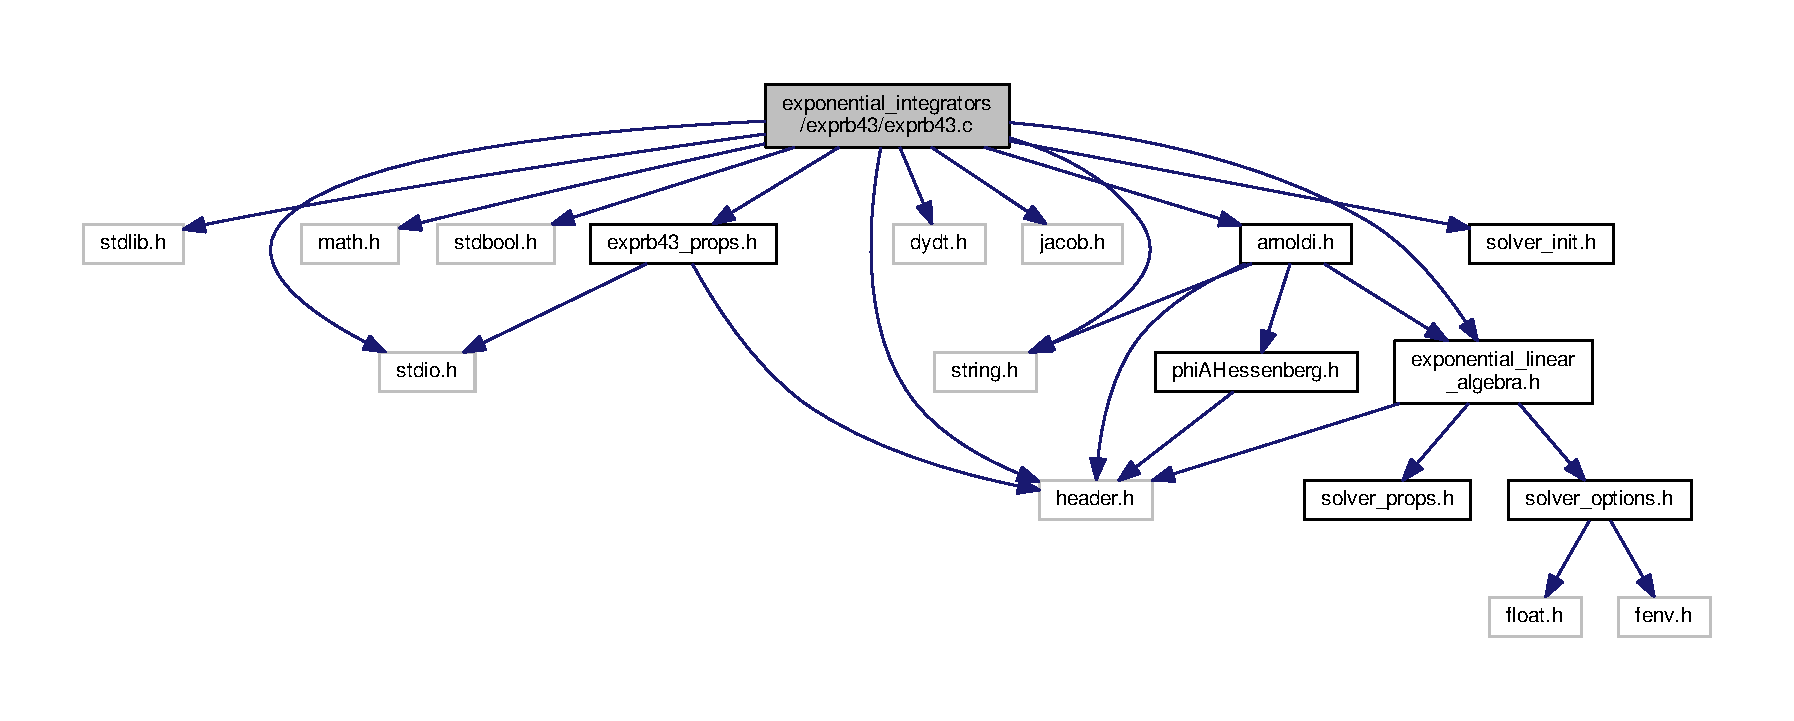
\includegraphics[width=350pt]{exprb43_8c__incl}
\end{center}
\end{figure}
\subsection*{Namespaces}
\begin{DoxyCompactItemize}
\item 
 \hyperlink{namespaceexprb43}{exprb43}
\end{DoxyCompactItemize}
\subsection*{Functions}
\begin{DoxyCompactItemize}
\item 
int \hyperlink{namespaceexprb43_a67d60af836938be17821d7ca32fa31fa}{exprb43\+::integrate} (const double t\+\_\+start, const double t\+\_\+end, const double pr, double $\ast$y)
\begin{DoxyCompactList}\small\item\em 4th-\/order exponential integrator function w/ adaptive Kyrlov subspace approximation \end{DoxyCompactList}\end{DoxyCompactItemize}


\subsection{Detailed Description}
A krylov subspace integrator using a 4th order (3rd-\/order embedded) exponential Rosenbrock method of Hochbruck et al. (2009) 

\begin{DoxyAuthor}{Author}
Nicholas J. Curtis 
\end{DoxyAuthor}
\begin{DoxyDate}{Date}
09/02/2014
\end{DoxyDate}
See full reference\+: M. Hochbruck, A. Ostermann, J. Schweitzer, Exponential Rosenbrock-\/type methods, S\+I\+AM J. Numer. Anal. 47 (1) (2009) 786–803. doi\+:10.\+1137/080717717.

N\+O\+TE\+: all matricies stored in column major format! 
\hypertarget{exprb43_8cu}{}\section{/home/nick/\+Dropbox/acceler\+Int/exponential\+\_\+integrators/exprb43/exprb43.cu File Reference}
\label{exprb43_8cu}\index{/home/nick/\+Dropbox/acceler\+Int/exponential\+\_\+integrators/exprb43/exprb43.\+cu@{/home/nick/\+Dropbox/acceler\+Int/exponential\+\_\+integrators/exprb43/exprb43.\+cu}}


A krylov subspace integrator using a 4th order (3rd-\/order embedded) exponential Rosenbrock method of Hochbruck et al. (2009)  


{\ttfamily \#include $<$stdlib.\+h$>$}\\*
{\ttfamily \#include $<$stdio.\+h$>$}\\*
{\ttfamily \#include $<$math.\+h$>$}\\*
{\ttfamily \#include $<$stdbool.\+h$>$}\\*
{\ttfamily \#include $<$cu\+Complex.\+h$>$}\\*
{\ttfamily \#include \char`\"{}header.\+cuh\char`\"{}}\\*
{\ttfamily \#include \char`\"{}solver\+\_\+options.\+cuh\char`\"{}}\\*
{\ttfamily \#include \char`\"{}solver\+\_\+props.\+cuh\char`\"{}}\\*
{\ttfamily \#include \char`\"{}dydt.\+cuh\char`\"{}}\\*
{\ttfamily \#include \char`\"{}jacob.\+cuh\char`\"{}}\\*
{\ttfamily \#include \char`\"{}exprb43\+\_\+props.\+cuh\char`\"{}}\\*
{\ttfamily \#include \char`\"{}arnoldi.\+cuh\char`\"{}}\\*
{\ttfamily \#include \char`\"{}exponential\+\_\+linear\+\_\+algebra.\+cuh\char`\"{}}\\*
{\ttfamily \#include \char`\"{}solver\+\_\+init.\+cuh\char`\"{}}\\*
{\ttfamily \#include \char`\"{}gpu\+\_\+macros.\+cuh\char`\"{}}\\*
Include dependency graph for exprb43.\+cu\+:
\nopagebreak
\begin{figure}[H]
\begin{center}
\leavevmode
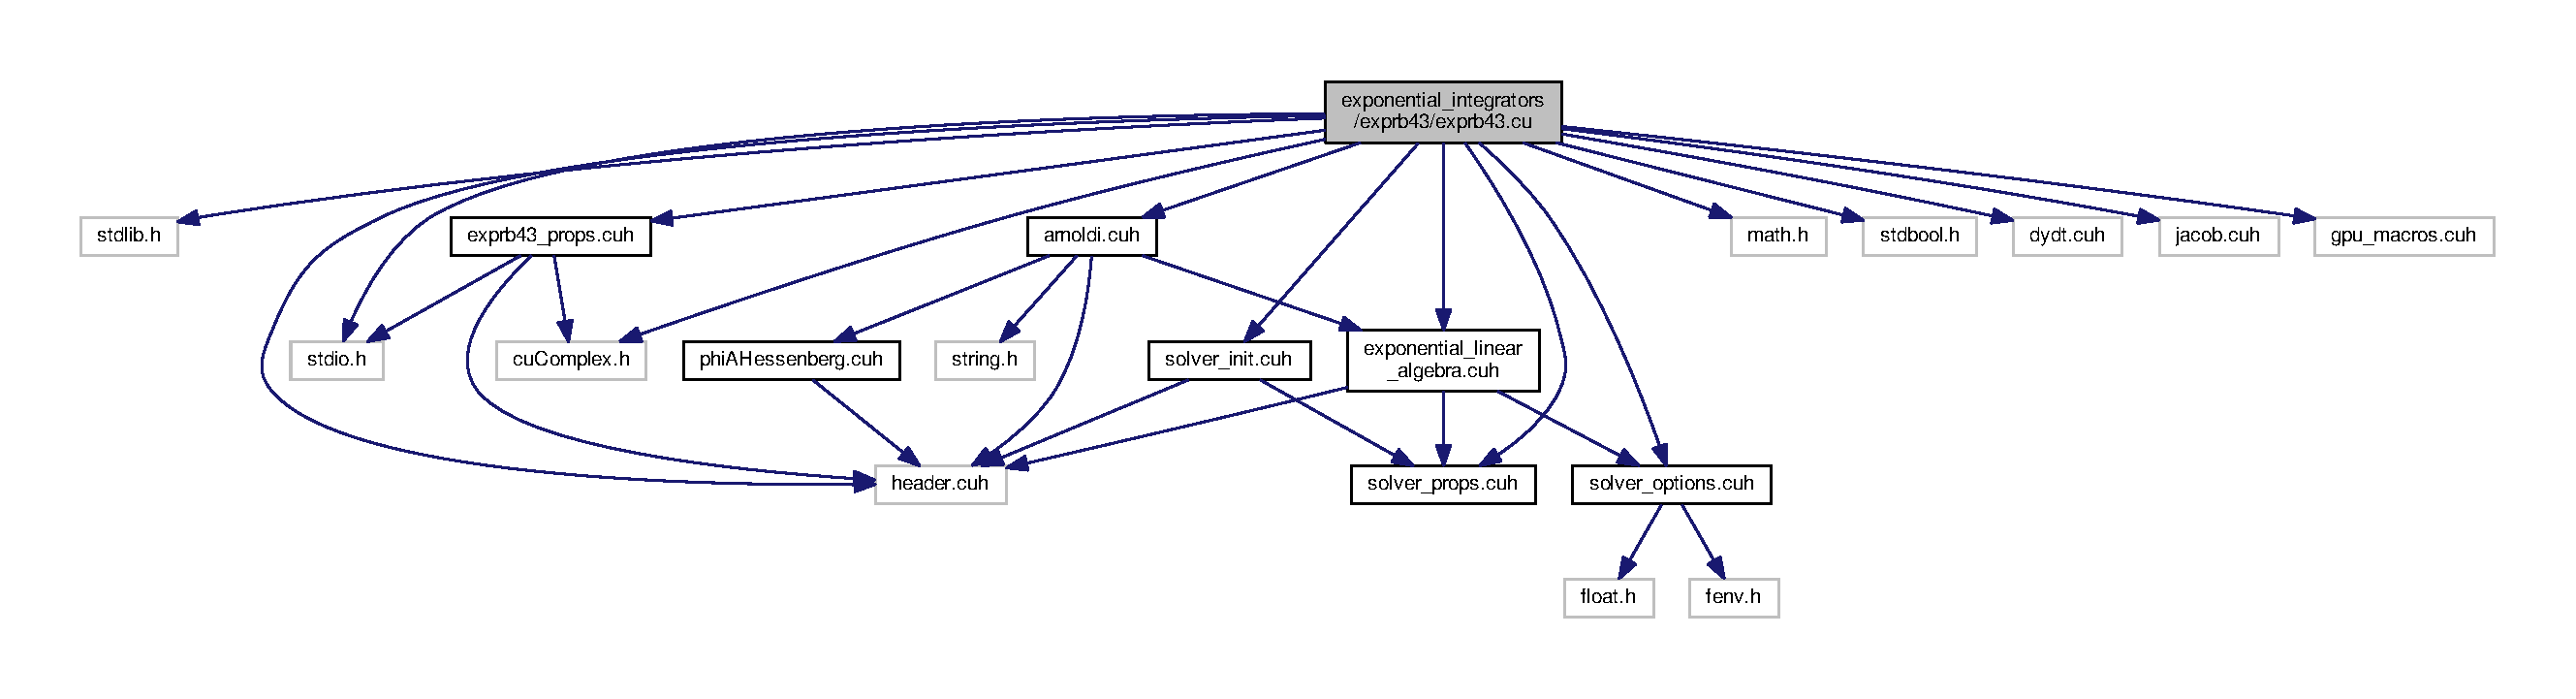
\includegraphics[width=350pt]{exprb43_8cu__incl}
\end{center}
\end{figure}
\subsection*{Namespaces}
\begin{DoxyCompactItemize}
\item 
 \hyperlink{namespaceexprb43cu}{exprb43cu}
\end{DoxyCompactItemize}
\subsection*{Functions}
\begin{DoxyCompactItemize}
\item 
\+\_\+\+\_\+device\+\_\+\+\_\+ void \hyperlink{namespaceexprb43cu_ad98c42138e12fe026951999e87b1ceb4}{exprb43cu\+::integrate} (const double t\+\_\+start, const double t\+\_\+end, const double pr, double $\ast$\+\_\+\+\_\+restrict\+\_\+\+\_\+ y, const mechanism\+\_\+memory $\ast$\+\_\+\+\_\+restrict\+\_\+\+\_\+ mech, const \hyperlink{structsolver__memory}{solver\+\_\+memory} $\ast$\+\_\+\+\_\+restrict\+\_\+\+\_\+ solver)
\end{DoxyCompactItemize}


\subsection{Detailed Description}
A krylov subspace integrator using a 4th order (3rd-\/order embedded) exponential Rosenbrock method of Hochbruck et al. (2009) 

\begin{DoxyAuthor}{Author}
Nicholas J. Curtis 
\end{DoxyAuthor}
\begin{DoxyDate}{Date}
09/02/2014
\end{DoxyDate}
See full reference\+: M. Hochbruck, A. Ostermann, J. Schweitzer, Exponential Rosenbrock-\/type methods, S\+I\+AM J. Numer. Anal. 47 (1) (2009) 786–803. doi\+:10.\+1137/080717717.

N\+O\+TE\+: all matricies stored in column major format! 
\hypertarget{exprb43__init_8c}{}\section{/home/nick/\+Dropbox/acceler\+Int/exponential\+\_\+integrators/exprb43/exprb43\+\_\+init.c File Reference}
\label{exprb43__init_8c}\index{/home/nick/\+Dropbox/acceler\+Int/exponential\+\_\+integrators/exprb43/exprb43\+\_\+init.\+c@{/home/nick/\+Dropbox/acceler\+Int/exponential\+\_\+integrators/exprb43/exprb43\+\_\+init.\+c}}


Implementation of the necessary initialization for the 4th order (3rd order embedded) Rosenbrock Solver.  


{\ttfamily \#include \char`\"{}rational\+\_\+approximant.\+h\char`\"{}}\\*
Include dependency graph for exprb43\+\_\+init.\+c\+:
\nopagebreak
\begin{figure}[H]
\begin{center}
\leavevmode
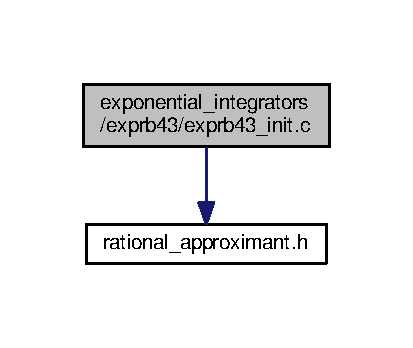
\includegraphics[width=249pt]{exprb43__init_8c__incl}
\end{center}
\end{figure}
\subsection*{Namespaces}
\begin{DoxyCompactItemize}
\item 
 \hyperlink{namespaceexprb43}{exprb43}
\end{DoxyCompactItemize}
\subsection*{Functions}
\begin{DoxyCompactItemize}
\item 
void \hyperlink{namespaceexprb43_adb214180d920bd67592be89b6264aa90}{exprb43\+::init\+\_\+solver\+\_\+log} ()
\begin{DoxyCompactList}\small\item\em Initializes the Krylov subspace logging files (if L\+O\+G\+\_\+\+O\+U\+T\+P\+UT is defined) \end{DoxyCompactList}\item 
void \hyperlink{namespaceexprb43_ad02d94a3cc25e03cf47a6903559f4262}{exprb43\+::solver\+\_\+log} ()
\begin{DoxyCompactList}\small\item\em Executes solver specific logging tasks. \end{DoxyCompactList}\item 
void \hyperlink{namespaceexprb43_a923d03974bd3461619b71ac8fb34abd8}{exprb43\+::initialize\+\_\+solver} (int num\+\_\+threads)
\begin{DoxyCompactList}\small\item\em Initializes the solver. \end{DoxyCompactList}\item 
const char $\ast$ \hyperlink{namespaceexprb43_a5357a692b80a08edee50c4073763422b}{exprb43\+::solver\+\_\+name} ()
\begin{DoxyCompactList}\small\item\em Returns a descriptive solver name. \end{DoxyCompactList}\item 
void \hyperlink{namespaceexprb43_ad7bbc3b8b5f2627e89908cdec0750523}{exprb43\+::cleanup\+\_\+solver} (int num\+\_\+threads)
\begin{DoxyCompactList}\small\item\em Cleans up the created solvers. \end{DoxyCompactList}\end{DoxyCompactItemize}


\subsection{Detailed Description}
Implementation of the necessary initialization for the 4th order (3rd order embedded) Rosenbrock Solver. 

\begin{DoxyAuthor}{Author}
Nicholas Curtis 
\end{DoxyAuthor}
\begin{DoxyDate}{Date}
03/09/2015 
\end{DoxyDate}

\hypertarget{exprb43__init_8cu}{}\section{exponential\+\_\+integrators/exprb43/exprb43\+\_\+init.cu File Reference}
\label{exprb43__init_8cu}\index{exponential\+\_\+integrators/exprb43/exprb43\+\_\+init.\+cu@{exponential\+\_\+integrators/exprb43/exprb43\+\_\+init.\+cu}}
{\ttfamily \#include \char`\"{}rational\+\_\+approximant.\+cuh\char`\"{}}\\*
{\ttfamily \#include \char`\"{}solver\+\_\+options.\+cuh\char`\"{}}\\*
{\ttfamily \#include \char`\"{}solver\+\_\+props.\+cuh\char`\"{}}\\*
{\ttfamily \#include \char`\"{}gpu\+\_\+macros.\+cuh\char`\"{}}\\*
Include dependency graph for exprb43\+\_\+init.\+cu\+:\nopagebreak
\begin{figure}[H]
\begin{center}
\leavevmode
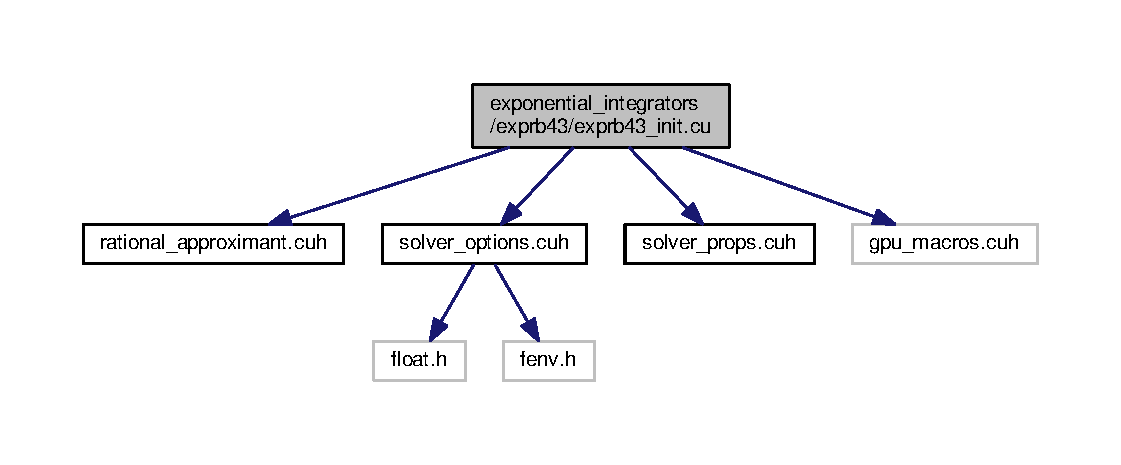
\includegraphics[width=350pt]{exprb43__init_8cu__incl}
\end{center}
\end{figure}
\subsection*{Namespaces}
\begin{DoxyCompactItemize}
\item 
 \hyperlink{namespaceexprb43cu}{exprb43cu}
\end{DoxyCompactItemize}
\subsection*{Functions}
\begin{DoxyCompactItemize}
\item 
const char $\ast$ \hyperlink{namespaceexprb43cu_adb32cc589856026fca36d47f1982ee00}{exprb43cu\+::solver\+\_\+name} ()
\begin{DoxyCompactList}\small\item\em Returns the E\+X\+P\+B43 solver name. \end{DoxyCompactList}\item 
void \hyperlink{namespaceexprb43cu_a77622bf304d732c5402474fe69dbb4a2}{exprb43cu\+::solver\+\_\+log} ()
\begin{DoxyCompactList}\small\item\em Logs errors, step-\/sizes, and krylov subspace size (if L\+O\+G\+\_\+\+O\+U\+T\+P\+UT is defined) \end{DoxyCompactList}\item 
void \hyperlink{namespaceexprb43cu_a61e02bb434629c817de6934d514fc96c}{exprb43cu\+::init\+\_\+solver\+\_\+log} ()
\begin{DoxyCompactList}\small\item\em Initializes the Krylov subspace logging files (if L\+O\+G\+\_\+\+O\+U\+T\+P\+UT is defined) \end{DoxyCompactList}\item 
size\+\_\+t \hyperlink{namespaceexprb43cu_ad837089abb4cfc3819786aad86440da0}{exprb43cu\+::required\+\_\+solver\+\_\+size} ()
\begin{DoxyCompactList}\small\item\em Returns the total size (in bytes) required for memory storage for a single G\+PU thread Used in calculation of the maximum number of possible G\+PU threads to launch, this method returns the size of the \hyperlink{structexprb43cu_1_1solver__memory}{solver\+\_\+memory} structure (per-\/\+G\+PU thread) \end{DoxyCompactList}\item 
void \hyperlink{namespaceexprb43cu_a411c61dc481c439d2a19e8f17ec5af63}{exprb43cu\+::create\+And\+Zero} (void $\ast$$\ast$ptr, size\+\_\+t size)
\item 
void \hyperlink{namespaceexprb43cu_a6c8137b2fd79c625faa2773ea26deb10}{exprb43cu\+::initialize\+\_\+solver} (int padded, \hyperlink{structsolver__memory}{solver\+\_\+memory} $\ast$$\ast$h\+\_\+mem, \hyperlink{structsolver__memory}{solver\+\_\+memory} $\ast$$\ast$d\+\_\+mem)
\begin{DoxyCompactList}\small\item\em Solves for the poles and residuals used for the Rational Approximants in the Krylov subspace methods and initializes \hyperlink{structexprb43cu_1_1solver__memory}{solver\+\_\+memory}. \end{DoxyCompactList}\item 
void \hyperlink{namespaceexprb43cu_a2a93d9ac22d074a6003cb959e74fae61}{exprb43cu\+::cleanup\+\_\+solver} (\hyperlink{structsolver__memory}{solver\+\_\+memory} $\ast$$\ast$h\+\_\+mem, \hyperlink{structsolver__memory}{solver\+\_\+memory} $\ast$$\ast$d\+\_\+mem)
\begin{DoxyCompactList}\small\item\em Cleans up solver memory, and closes Krylov subspace logfiles (if L\+O\+G\+\_\+\+O\+U\+T\+P\+UT is defined) \end{DoxyCompactList}\end{DoxyCompactItemize}

\hypertarget{exprb43__props_8c}{}\section{exponential\+\_\+integrators/exprb43/exprb43\+\_\+props.c File Reference}
\label{exprb43__props_8c}\index{exponential\+\_\+integrators/exprb43/exprb43\+\_\+props.\+c@{exponential\+\_\+integrators/exprb43/exprb43\+\_\+props.\+c}}


Contains error checking for E\+X\+P\+R\+B43 return codes.  


{\ttfamily \#include \char`\"{}exprb43\+\_\+props.\+h\char`\"{}}\\*
Include dependency graph for exprb43\+\_\+props.\+c\+:\nopagebreak
\begin{figure}[H]
\begin{center}
\leavevmode
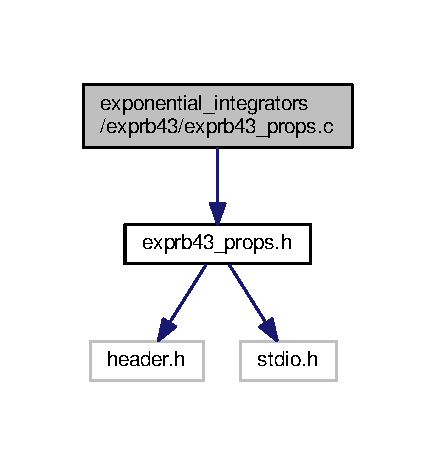
\includegraphics[width=209pt]{exprb43__props_8c__incl}
\end{center}
\end{figure}
\subsection*{Namespaces}
\begin{DoxyCompactItemize}
\item 
 \hyperlink{namespaceexprb43}{exprb43}
\end{DoxyCompactItemize}
\subsection*{Functions}
\begin{DoxyCompactItemize}
\item 
void \hyperlink{namespaceexprb43_aa165b73c13e21b53f0713c4c5ec5fd7c}{exprb43\+::check\+\_\+error} (int tid, int code)
\begin{DoxyCompactList}\small\item\em Checks the return code of the given thread (I\+VP) for an error, and exits if found. \end{DoxyCompactList}\end{DoxyCompactItemize}


\subsection{Detailed Description}
Contains error checking for E\+X\+P\+R\+B43 return codes. 

\begin{DoxyAuthor}{Author}
Nicholas J. Curtis 
\end{DoxyAuthor}
\begin{DoxyDate}{Date}
09/02/2014 
\end{DoxyDate}

\hypertarget{exprb43__props_8cu}{}\section{exponential\+\_\+integrators/exprb43/exprb43\+\_\+props.cu File Reference}
\label{exprb43__props_8cu}\index{exponential\+\_\+integrators/exprb43/exprb43\+\_\+props.\+cu@{exponential\+\_\+integrators/exprb43/exprb43\+\_\+props.\+cu}}


Error checking for the E\+X\+P\+R\+B43 algorithm.  


{\ttfamily \#include \char`\"{}exprb43\+\_\+props.\+cuh\char`\"{}}\\*
Include dependency graph for exprb43\+\_\+props.\+cu\+:\nopagebreak
\begin{figure}[H]
\begin{center}
\leavevmode
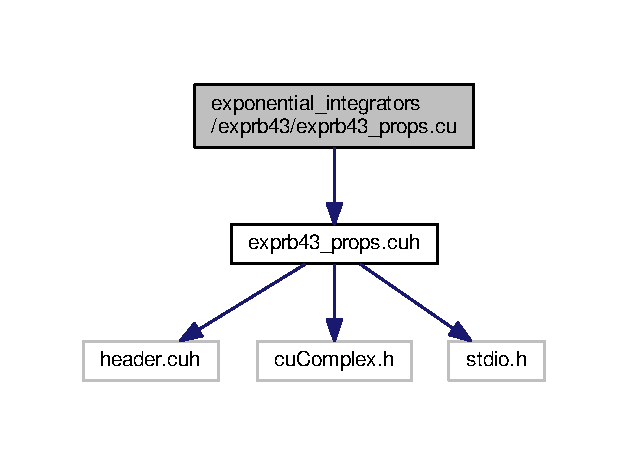
\includegraphics[width=302pt]{exprb43__props_8cu__incl}
\end{center}
\end{figure}
\subsection*{Namespaces}
\begin{DoxyCompactItemize}
\item 
 \hyperlink{namespaceexprb43cu}{exprb43cu}
\end{DoxyCompactItemize}
\subsection*{Functions}
\begin{DoxyCompactItemize}
\item 
\+\_\+\+\_\+host\+\_\+\+\_\+ void \hyperlink{namespaceexprb43cu_aea2a90f02f654f5e485a7bea9c34985f}{exprb43cu\+::check\+\_\+error} (int num\+\_\+cond, int $\ast$codes)
\end{DoxyCompactItemize}


\subsection{Detailed Description}
Error checking for the E\+X\+P\+R\+B43 algorithm. 

\begin{DoxyAuthor}{Author}
Nicholas Curtis 
\end{DoxyAuthor}
\begin{DoxyDate}{Date}
03/10/2015 
\end{DoxyDate}

\hypertarget{exprb43__props_8cuh}{}\section{/home/nick/\+Dropbox/acceler\+Int/exponential\+\_\+integrators/exprb43/exprb43\+\_\+props.cuh File Reference}
\label{exprb43__props_8cuh}\index{/home/nick/\+Dropbox/acceler\+Int/exponential\+\_\+integrators/exprb43/exprb43\+\_\+props.\+cuh@{/home/nick/\+Dropbox/acceler\+Int/exponential\+\_\+integrators/exprb43/exprb43\+\_\+props.\+cuh}}


Various macros controlling behaviour of R\+B43 algorithm.  


{\ttfamily \#include \char`\"{}header.\+cuh\char`\"{}}\\*
{\ttfamily \#include $<$cu\+Complex.\+h$>$}\\*
{\ttfamily \#include $<$stdio.\+h$>$}\\*
Include dependency graph for exprb43\+\_\+props.\+cuh\+:
\nopagebreak
\begin{figure}[H]
\begin{center}
\leavevmode
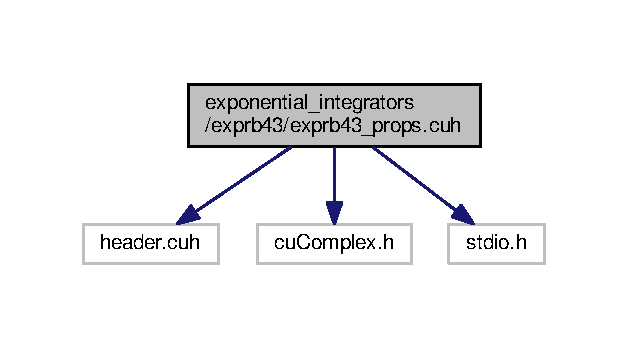
\includegraphics[width=302pt]{exprb43__props_8cuh__incl}
\end{center}
\end{figure}
This graph shows which files directly or indirectly include this file\+:
\nopagebreak
\begin{figure}[H]
\begin{center}
\leavevmode
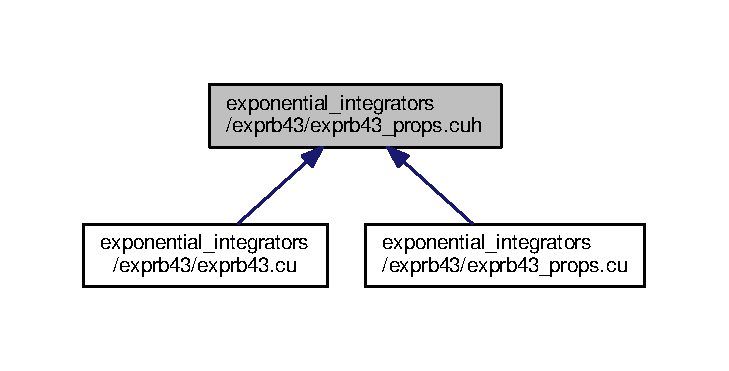
\includegraphics[width=350pt]{exprb43__props_8cuh__dep__incl}
\end{center}
\end{figure}
\subsection*{Classes}
\begin{DoxyCompactItemize}
\item 
struct \hyperlink{structexprb43cu_1_1solver__memory}{exprb43cu\+::solver\+\_\+memory}
\end{DoxyCompactItemize}
\subsection*{Namespaces}
\begin{DoxyCompactItemize}
\item 
 \hyperlink{namespaceexprb43cu}{exprb43cu}
\end{DoxyCompactItemize}
\subsection*{Macros}
\begin{DoxyCompactItemize}
\item 
\#define \hyperlink{exprb43__props_8cuh_a662425e5e115738094e7136bcfea795f}{R\+B43\+\_\+\+P\+R\+O\+P\+S\+\_\+\+C\+UH}
\item 
\#define \hyperlink{exprb43__props_8cuh_a2748566f4c443ee77aa831e63dbb5ebe}{P}~4
\begin{DoxyCompactList}\small\item\em max order of the phi functions (for error estimation) \end{DoxyCompactList}\item 
\#define \hyperlink{exprb43__props_8cuh_ac5232262b17b940a7b54e6e56439aa24}{O\+RD}~3.\+0
\begin{DoxyCompactList}\small\item\em order of embedded methods \end{DoxyCompactList}\item 
\#define \hyperlink{exprb43__props_8cuh_a61819141b0164a35f4d791b0e696721f}{M\+\_\+\+M\+AX}~N\+SP
\begin{DoxyCompactList}\small\item\em maximum Krylov dimension (without phi order) \end{DoxyCompactList}\item 
\#define \hyperlink{exprb43__props_8cuh_a351d54267048643c4365f6a24641d0cf}{S\+T\+R\+I\+DE}~(\hyperlink{exprb43__props_8h_a61819141b0164a35f4d791b0e696721f}{M\+\_\+\+M\+AX} + \hyperlink{exprb43__props_8h_a2748566f4c443ee77aa831e63dbb5ebe}{P})
\begin{DoxyCompactList}\small\item\em Krylov matrix stride. \end{DoxyCompactList}\item 
\#define \hyperlink{exprb43__props_8cuh_aa0414caef00a64a51d4c6c0711d9e70a}{M\+A\+X\+\_\+\+S\+T\+E\+PS}~(100000)
\begin{DoxyCompactList}\small\item\em Maximum allowed internal timesteps per integration step. \end{DoxyCompactList}\item 
\#define \hyperlink{exprb43__props_8cuh_a0f51553c710580b9899756f7ad472c93}{M\+A\+X\+\_\+\+C\+O\+N\+S\+E\+C\+U\+T\+I\+V\+E\+\_\+\+E\+R\+R\+O\+RS}~(5)
\begin{DoxyCompactList}\small\item\em Number of consecutive errors on internal integration steps allowed before exit. \end{DoxyCompactList}\item 
\#define \hyperlink{group__exprb43cu__ErrCodes_gabd83bc0f9f475a2189a4db4a08b790ca}{E\+C\+\_\+success}~(0)
\begin{DoxyCompactList}\small\item\em Successful integration step. \end{DoxyCompactList}\item 
\#define \hyperlink{group__exprb43cu__ErrCodes_gae0287841c08f86f5709660fd731615ad}{E\+C\+\_\+consecutive\+\_\+steps}~(1)
\begin{DoxyCompactList}\small\item\em Maximum consecutive errors on internal integration steps reached. \end{DoxyCompactList}\item 
\#define \hyperlink{group__exprb43cu__ErrCodes_ga0f0275d9851ab5c19b79a963d5084df3}{E\+C\+\_\+max\+\_\+steps\+\_\+exceeded}~(2)
\begin{DoxyCompactList}\small\item\em Maximum number of internal integration steps reached. \end{DoxyCompactList}\item 
\#define \hyperlink{group__exprb43cu__ErrCodes_ga9326efd544880e2683c4453365ca2704}{E\+C\+\_\+h\+\_\+plus\+\_\+t\+\_\+equals\+\_\+h}~(3)
\begin{DoxyCompactList}\small\item\em Timestep reduced such that update would have no effect on simulation time. \end{DoxyCompactList}\end{DoxyCompactItemize}


\subsection{Detailed Description}
Various macros controlling behaviour of R\+B43 algorithm. 

\begin{DoxyAuthor}{Author}
Nicholas Curtis 
\end{DoxyAuthor}
\begin{DoxyDate}{Date}
03/10/2015 
\end{DoxyDate}


\subsection{Macro Definition Documentation}
\index{exprb43\+\_\+props.\+cuh@{exprb43\+\_\+props.\+cuh}!M\+\_\+\+M\+AX@{M\+\_\+\+M\+AX}}
\index{M\+\_\+\+M\+AX@{M\+\_\+\+M\+AX}!exprb43\+\_\+props.\+cuh@{exprb43\+\_\+props.\+cuh}}
\subsubsection[{\texorpdfstring{M\+\_\+\+M\+AX}{M_MAX}}]{\setlength{\rightskip}{0pt plus 5cm}\#define M\+\_\+\+M\+AX~N\+SP}\hypertarget{exprb43__props_8cuh_a61819141b0164a35f4d791b0e696721f}{}\label{exprb43__props_8cuh_a61819141b0164a35f4d791b0e696721f}


maximum Krylov dimension (without phi order) 

\index{exprb43\+\_\+props.\+cuh@{exprb43\+\_\+props.\+cuh}!M\+A\+X\+\_\+\+C\+O\+N\+S\+E\+C\+U\+T\+I\+V\+E\+\_\+\+E\+R\+R\+O\+RS@{M\+A\+X\+\_\+\+C\+O\+N\+S\+E\+C\+U\+T\+I\+V\+E\+\_\+\+E\+R\+R\+O\+RS}}
\index{M\+A\+X\+\_\+\+C\+O\+N\+S\+E\+C\+U\+T\+I\+V\+E\+\_\+\+E\+R\+R\+O\+RS@{M\+A\+X\+\_\+\+C\+O\+N\+S\+E\+C\+U\+T\+I\+V\+E\+\_\+\+E\+R\+R\+O\+RS}!exprb43\+\_\+props.\+cuh@{exprb43\+\_\+props.\+cuh}}
\subsubsection[{\texorpdfstring{M\+A\+X\+\_\+\+C\+O\+N\+S\+E\+C\+U\+T\+I\+V\+E\+\_\+\+E\+R\+R\+O\+RS}{MAX_CONSECUTIVE_ERRORS}}]{\setlength{\rightskip}{0pt plus 5cm}\#define M\+A\+X\+\_\+\+C\+O\+N\+S\+E\+C\+U\+T\+I\+V\+E\+\_\+\+E\+R\+R\+O\+RS~(5)}\hypertarget{exprb43__props_8cuh_a0f51553c710580b9899756f7ad472c93}{}\label{exprb43__props_8cuh_a0f51553c710580b9899756f7ad472c93}


Number of consecutive errors on internal integration steps allowed before exit. 

\index{exprb43\+\_\+props.\+cuh@{exprb43\+\_\+props.\+cuh}!M\+A\+X\+\_\+\+S\+T\+E\+PS@{M\+A\+X\+\_\+\+S\+T\+E\+PS}}
\index{M\+A\+X\+\_\+\+S\+T\+E\+PS@{M\+A\+X\+\_\+\+S\+T\+E\+PS}!exprb43\+\_\+props.\+cuh@{exprb43\+\_\+props.\+cuh}}
\subsubsection[{\texorpdfstring{M\+A\+X\+\_\+\+S\+T\+E\+PS}{MAX_STEPS}}]{\setlength{\rightskip}{0pt plus 5cm}\#define M\+A\+X\+\_\+\+S\+T\+E\+PS~(100000)}\hypertarget{exprb43__props_8cuh_aa0414caef00a64a51d4c6c0711d9e70a}{}\label{exprb43__props_8cuh_aa0414caef00a64a51d4c6c0711d9e70a}


Maximum allowed internal timesteps per integration step. 

\index{exprb43\+\_\+props.\+cuh@{exprb43\+\_\+props.\+cuh}!O\+RD@{O\+RD}}
\index{O\+RD@{O\+RD}!exprb43\+\_\+props.\+cuh@{exprb43\+\_\+props.\+cuh}}
\subsubsection[{\texorpdfstring{O\+RD}{ORD}}]{\setlength{\rightskip}{0pt plus 5cm}\#define O\+RD~3.\+0}\hypertarget{exprb43__props_8cuh_ac5232262b17b940a7b54e6e56439aa24}{}\label{exprb43__props_8cuh_ac5232262b17b940a7b54e6e56439aa24}


order of embedded methods 

\index{exprb43\+\_\+props.\+cuh@{exprb43\+\_\+props.\+cuh}!P@{P}}
\index{P@{P}!exprb43\+\_\+props.\+cuh@{exprb43\+\_\+props.\+cuh}}
\subsubsection[{\texorpdfstring{P}{P}}]{\setlength{\rightskip}{0pt plus 5cm}\#define P~4}\hypertarget{exprb43__props_8cuh_a2748566f4c443ee77aa831e63dbb5ebe}{}\label{exprb43__props_8cuh_a2748566f4c443ee77aa831e63dbb5ebe}


max order of the phi functions (for error estimation) 

\index{exprb43\+\_\+props.\+cuh@{exprb43\+\_\+props.\+cuh}!R\+B43\+\_\+\+P\+R\+O\+P\+S\+\_\+\+C\+UH@{R\+B43\+\_\+\+P\+R\+O\+P\+S\+\_\+\+C\+UH}}
\index{R\+B43\+\_\+\+P\+R\+O\+P\+S\+\_\+\+C\+UH@{R\+B43\+\_\+\+P\+R\+O\+P\+S\+\_\+\+C\+UH}!exprb43\+\_\+props.\+cuh@{exprb43\+\_\+props.\+cuh}}
\subsubsection[{\texorpdfstring{R\+B43\+\_\+\+P\+R\+O\+P\+S\+\_\+\+C\+UH}{RB43_PROPS_CUH}}]{\setlength{\rightskip}{0pt plus 5cm}\#define R\+B43\+\_\+\+P\+R\+O\+P\+S\+\_\+\+C\+UH}\hypertarget{exprb43__props_8cuh_a662425e5e115738094e7136bcfea795f}{}\label{exprb43__props_8cuh_a662425e5e115738094e7136bcfea795f}
\index{exprb43\+\_\+props.\+cuh@{exprb43\+\_\+props.\+cuh}!S\+T\+R\+I\+DE@{S\+T\+R\+I\+DE}}
\index{S\+T\+R\+I\+DE@{S\+T\+R\+I\+DE}!exprb43\+\_\+props.\+cuh@{exprb43\+\_\+props.\+cuh}}
\subsubsection[{\texorpdfstring{S\+T\+R\+I\+DE}{STRIDE}}]{\setlength{\rightskip}{0pt plus 5cm}\#define S\+T\+R\+I\+DE~({\bf M\+\_\+\+M\+AX} + {\bf P})}\hypertarget{exprb43__props_8cuh_a351d54267048643c4365f6a24641d0cf}{}\label{exprb43__props_8cuh_a351d54267048643c4365f6a24641d0cf}


Krylov matrix stride. 


\hypertarget{exprb43__props_8h}{}\section{exponential\+\_\+integrators/exprb43/exprb43\+\_\+props.h File Reference}
\label{exprb43__props_8h}\index{exponential\+\_\+integrators/exprb43/exprb43\+\_\+props.\+h@{exponential\+\_\+integrators/exprb43/exprb43\+\_\+props.\+h}}


Various macros controlling behaviour of E\+X\+P\+R\+B43 algorithm.  


{\ttfamily \#include \char`\"{}header.\+h\char`\"{}}\\*
{\ttfamily \#include $<$stdio.\+h$>$}\\*
Include dependency graph for exprb43\+\_\+props.\+h\+:\nopagebreak
\begin{figure}[H]
\begin{center}
\leavevmode
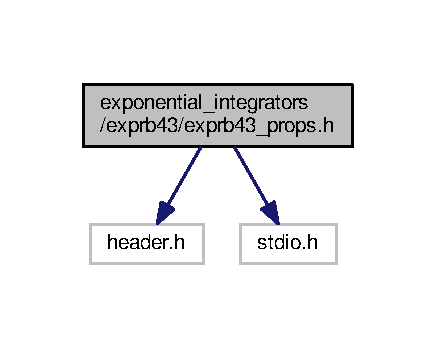
\includegraphics[width=209pt]{exprb43__props_8h__incl}
\end{center}
\end{figure}
This graph shows which files directly or indirectly include this file\+:\nopagebreak
\begin{figure}[H]
\begin{center}
\leavevmode
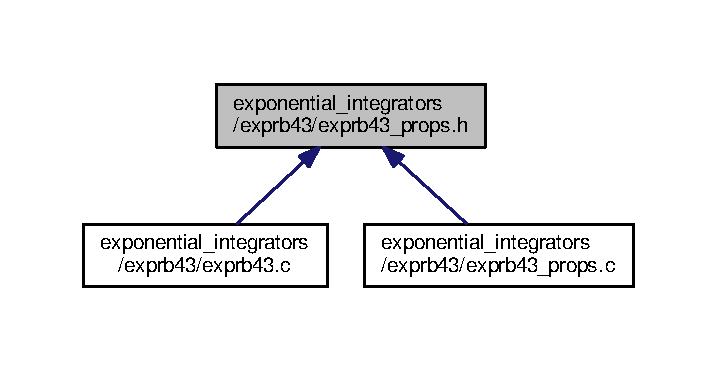
\includegraphics[width=344pt]{exprb43__props_8h__dep__incl}
\end{center}
\end{figure}
\subsection*{Namespaces}
\begin{DoxyCompactItemize}
\item 
 \hyperlink{namespaceexprb43}{exprb43}
\end{DoxyCompactItemize}
\subsection*{Macros}
\begin{DoxyCompactItemize}
\item 
\#define \hyperlink{exprb43__props_8h_a2748566f4c443ee77aa831e63dbb5ebe}{P}~4
\begin{DoxyCompactList}\small\item\em max order of the phi functions (for error estimation) \end{DoxyCompactList}\item 
\#define \hyperlink{exprb43__props_8h_ac5232262b17b940a7b54e6e56439aa24}{O\+RD}~3.\+0
\begin{DoxyCompactList}\small\item\em order of embedded methods \end{DoxyCompactList}\item 
\#define \hyperlink{exprb43__props_8h_a61819141b0164a35f4d791b0e696721f}{M\+\_\+\+M\+AX}~N\+SP
\begin{DoxyCompactList}\small\item\em maximum Krylov dimension (without phi order) \end{DoxyCompactList}\item 
\#define \hyperlink{exprb43__props_8h_a351d54267048643c4365f6a24641d0cf}{S\+T\+R\+I\+DE}~(\hyperlink{exprb43__props_8h_a61819141b0164a35f4d791b0e696721f}{M\+\_\+\+M\+AX} + \hyperlink{exprb43__props_8h_a2748566f4c443ee77aa831e63dbb5ebe}{P})
\begin{DoxyCompactList}\small\item\em Krylov matrix stride. \end{DoxyCompactList}\item 
\#define \hyperlink{exprb43__props_8h_aa0414caef00a64a51d4c6c0711d9e70a}{M\+A\+X\+\_\+\+S\+T\+E\+PS}~(100000)
\begin{DoxyCompactList}\small\item\em Maximum allowed internal timesteps per integration step. \end{DoxyCompactList}\item 
\#define \hyperlink{exprb43__props_8h_a0f51553c710580b9899756f7ad472c93}{M\+A\+X\+\_\+\+C\+O\+N\+S\+E\+C\+U\+T\+I\+V\+E\+\_\+\+E\+R\+R\+O\+RS}~(5)
\begin{DoxyCompactList}\small\item\em Number of consecutive errors on internal integration steps allowed before exit. \end{DoxyCompactList}\item 
\#define \hyperlink{group__exprb43__ErrCodes_gabd83bc0f9f475a2189a4db4a08b790ca}{E\+C\+\_\+success}~(0)
\begin{DoxyCompactList}\small\item\em Successful integration step. \end{DoxyCompactList}\item 
\#define \hyperlink{group__exprb43__ErrCodes_gae0287841c08f86f5709660fd731615ad}{E\+C\+\_\+consecutive\+\_\+steps}~(1)
\begin{DoxyCompactList}\small\item\em Maximum consecutive errors on internal integration steps reached. \end{DoxyCompactList}\item 
\#define \hyperlink{group__exprb43__ErrCodes_ga0f0275d9851ab5c19b79a963d5084df3}{E\+C\+\_\+max\+\_\+steps\+\_\+exceeded}~(2)
\begin{DoxyCompactList}\small\item\em Maximum number of internal integration steps reached. \end{DoxyCompactList}\item 
\#define \hyperlink{group__exprb43__ErrCodes_ga9326efd544880e2683c4453365ca2704}{E\+C\+\_\+h\+\_\+plus\+\_\+t\+\_\+equals\+\_\+h}~(3)
\begin{DoxyCompactList}\small\item\em Timestep reduced such that update would have no effect on simulation time. \end{DoxyCompactList}\end{DoxyCompactItemize}


\subsection{Detailed Description}
Various macros controlling behaviour of E\+X\+P\+R\+B43 algorithm. 

\begin{DoxyAuthor}{Author}
Nicholas Curtis 
\end{DoxyAuthor}
\begin{DoxyDate}{Date}
03/10/2015 
\end{DoxyDate}


\subsection{Macro Definition Documentation}
\index{exprb43\+\_\+props.\+h@{exprb43\+\_\+props.\+h}!M\+\_\+\+M\+AX@{M\+\_\+\+M\+AX}}
\index{M\+\_\+\+M\+AX@{M\+\_\+\+M\+AX}!exprb43\+\_\+props.\+h@{exprb43\+\_\+props.\+h}}
\subsubsection[{\texorpdfstring{M\+\_\+\+M\+AX}{M_MAX}}]{\setlength{\rightskip}{0pt plus 5cm}\#define M\+\_\+\+M\+AX~N\+SP}\hypertarget{exprb43__props_8h_a61819141b0164a35f4d791b0e696721f}{}\label{exprb43__props_8h_a61819141b0164a35f4d791b0e696721f}


maximum Krylov dimension (without phi order) 

\index{exprb43\+\_\+props.\+h@{exprb43\+\_\+props.\+h}!M\+A\+X\+\_\+\+C\+O\+N\+S\+E\+C\+U\+T\+I\+V\+E\+\_\+\+E\+R\+R\+O\+RS@{M\+A\+X\+\_\+\+C\+O\+N\+S\+E\+C\+U\+T\+I\+V\+E\+\_\+\+E\+R\+R\+O\+RS}}
\index{M\+A\+X\+\_\+\+C\+O\+N\+S\+E\+C\+U\+T\+I\+V\+E\+\_\+\+E\+R\+R\+O\+RS@{M\+A\+X\+\_\+\+C\+O\+N\+S\+E\+C\+U\+T\+I\+V\+E\+\_\+\+E\+R\+R\+O\+RS}!exprb43\+\_\+props.\+h@{exprb43\+\_\+props.\+h}}
\subsubsection[{\texorpdfstring{M\+A\+X\+\_\+\+C\+O\+N\+S\+E\+C\+U\+T\+I\+V\+E\+\_\+\+E\+R\+R\+O\+RS}{MAX_CONSECUTIVE_ERRORS}}]{\setlength{\rightskip}{0pt plus 5cm}\#define M\+A\+X\+\_\+\+C\+O\+N\+S\+E\+C\+U\+T\+I\+V\+E\+\_\+\+E\+R\+R\+O\+RS~(5)}\hypertarget{exprb43__props_8h_a0f51553c710580b9899756f7ad472c93}{}\label{exprb43__props_8h_a0f51553c710580b9899756f7ad472c93}


Number of consecutive errors on internal integration steps allowed before exit. 

\index{exprb43\+\_\+props.\+h@{exprb43\+\_\+props.\+h}!M\+A\+X\+\_\+\+S\+T\+E\+PS@{M\+A\+X\+\_\+\+S\+T\+E\+PS}}
\index{M\+A\+X\+\_\+\+S\+T\+E\+PS@{M\+A\+X\+\_\+\+S\+T\+E\+PS}!exprb43\+\_\+props.\+h@{exprb43\+\_\+props.\+h}}
\subsubsection[{\texorpdfstring{M\+A\+X\+\_\+\+S\+T\+E\+PS}{MAX_STEPS}}]{\setlength{\rightskip}{0pt plus 5cm}\#define M\+A\+X\+\_\+\+S\+T\+E\+PS~(100000)}\hypertarget{exprb43__props_8h_aa0414caef00a64a51d4c6c0711d9e70a}{}\label{exprb43__props_8h_aa0414caef00a64a51d4c6c0711d9e70a}


Maximum allowed internal timesteps per integration step. 

\index{exprb43\+\_\+props.\+h@{exprb43\+\_\+props.\+h}!O\+RD@{O\+RD}}
\index{O\+RD@{O\+RD}!exprb43\+\_\+props.\+h@{exprb43\+\_\+props.\+h}}
\subsubsection[{\texorpdfstring{O\+RD}{ORD}}]{\setlength{\rightskip}{0pt plus 5cm}\#define O\+RD~3.\+0}\hypertarget{exprb43__props_8h_ac5232262b17b940a7b54e6e56439aa24}{}\label{exprb43__props_8h_ac5232262b17b940a7b54e6e56439aa24}


order of embedded methods 

\index{exprb43\+\_\+props.\+h@{exprb43\+\_\+props.\+h}!P@{P}}
\index{P@{P}!exprb43\+\_\+props.\+h@{exprb43\+\_\+props.\+h}}
\subsubsection[{\texorpdfstring{P}{P}}]{\setlength{\rightskip}{0pt plus 5cm}\#define P~4}\hypertarget{exprb43__props_8h_a2748566f4c443ee77aa831e63dbb5ebe}{}\label{exprb43__props_8h_a2748566f4c443ee77aa831e63dbb5ebe}


max order of the phi functions (for error estimation) 

\index{exprb43\+\_\+props.\+h@{exprb43\+\_\+props.\+h}!S\+T\+R\+I\+DE@{S\+T\+R\+I\+DE}}
\index{S\+T\+R\+I\+DE@{S\+T\+R\+I\+DE}!exprb43\+\_\+props.\+h@{exprb43\+\_\+props.\+h}}
\subsubsection[{\texorpdfstring{S\+T\+R\+I\+DE}{STRIDE}}]{\setlength{\rightskip}{0pt plus 5cm}\#define S\+T\+R\+I\+DE~({\bf M\+\_\+\+M\+AX} + {\bf P})}\hypertarget{exprb43__props_8h_a351d54267048643c4365f6a24641d0cf}{}\label{exprb43__props_8h_a351d54267048643c4365f6a24641d0cf}


Krylov matrix stride. 


\hypertarget{linear-algebra_8c}{}\section{exponential\+\_\+integrators/linear-\/algebra.c File Reference}
\label{linear-algebra_8c}\index{exponential\+\_\+integrators/linear-\/algebra.\+c@{exponential\+\_\+integrators/linear-\/algebra.\+c}}


Various linear algebra routines needed for the Carathéodory-\/\+Fejér method.  


{\ttfamily \#include $<$stdlib.\+h$>$}\\*
{\ttfamily \#include $<$stdio.\+h$>$}\\*
{\ttfamily \#include $<$math.\+h$>$}\\*
{\ttfamily \#include $<$float.\+h$>$}\\*
{\ttfamily \#include $<$string.\+h$>$}\\*
{\ttfamily \#include $<$complex.\+h$>$}\\*
Include dependency graph for linear-\/algebra.c\+:\nopagebreak
\begin{figure}[H]
\begin{center}
\leavevmode
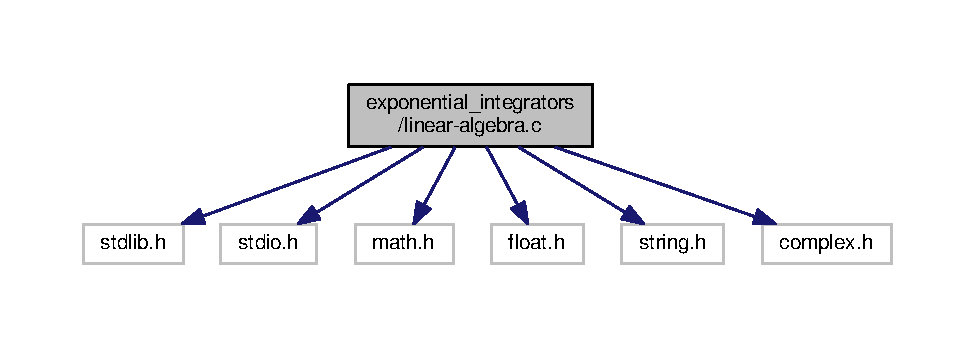
\includegraphics[width=350pt]{linear-algebra_8c__incl}
\end{center}
\end{figure}
\subsection*{Functions}
\begin{DoxyCompactItemize}
\item 
void \hyperlink{linear-algebra_8c_a2f33ac7496b7cd6fed5b44188e4aff1e}{get\+Inverse\+Complex} (int n, double complex $\ast$A)
\begin{DoxyCompactList}\small\item\em Interface function to L\+A\+P\+A\+CK matrix inversion subroutine. \end{DoxyCompactList}\item 
void \hyperlink{linear-algebra_8c_abe341bea743e72f19228e55d3fc02170}{lin\+Solve\+Complex} (int n, double complex $\ast$A, double complex $\ast$B, double complex $\ast$x)
\begin{DoxyCompactList}\small\item\em Solves the complex linear system Ax = B. \end{DoxyCompactList}\item 
void \hyperlink{linear-algebra_8c_ab95d3c92732d7711d9446fb25e0c6369}{roots} (int n, double $\ast$v, double complex $\ast$rt)
\begin{DoxyCompactList}\small\item\em Polynomial root finding function. \end{DoxyCompactList}\item 
void \hyperlink{linear-algebra_8c_a636107312a1724ef2534975b2ad05a83}{svd} (int n, double $\ast$A, double $\ast$S, double $\ast$U, double $\ast$V)
\begin{DoxyCompactList}\small\item\em Singular value decomposition function. \end{DoxyCompactList}\end{DoxyCompactItemize}


\subsection{Detailed Description}
Various linear algebra routines needed for the Carathéodory-\/\+Fejér method. 



\subsection{Function Documentation}
\index{linear-\/algebra.\+c@{linear-\/algebra.\+c}!get\+Inverse\+Complex@{get\+Inverse\+Complex}}
\index{get\+Inverse\+Complex@{get\+Inverse\+Complex}!linear-\/algebra.\+c@{linear-\/algebra.\+c}}
\subsubsection[{\texorpdfstring{get\+Inverse\+Complex(int n, double complex $\ast$\+A)}{getInverseComplex(int n, double complex *A)}}]{\setlength{\rightskip}{0pt plus 5cm}void get\+Inverse\+Complex (
\begin{DoxyParamCaption}
\item[{int}]{n, }
\item[{double complex $\ast$}]{A}
\end{DoxyParamCaption}
)}\hypertarget{linear-algebra_8c_a2f33ac7496b7cd6fed5b44188e4aff1e}{}\label{linear-algebra_8c_a2f33ac7496b7cd6fed5b44188e4aff1e}


Interface function to L\+A\+P\+A\+CK matrix inversion subroutine. 

Performs inversion of square matrix. Uses L\+A\+P\+A\+CK subroutines D\+G\+E\+T\+RF and D\+G\+E\+T\+RI.


\begin{DoxyParams}[1]{Parameters}
\mbox{\tt in}  & {\em n} & order of matrix \\
\hline
\mbox{\tt in}  & {\em A} & the input matrix, size n$\ast$n \\
\hline
\end{DoxyParams}
\begin{DoxyReturn}{Returns}
info success/fail integer flag 
\end{DoxyReturn}
\index{linear-\/algebra.\+c@{linear-\/algebra.\+c}!lin\+Solve\+Complex@{lin\+Solve\+Complex}}
\index{lin\+Solve\+Complex@{lin\+Solve\+Complex}!linear-\/algebra.\+c@{linear-\/algebra.\+c}}
\subsubsection[{\texorpdfstring{lin\+Solve\+Complex(int n, double complex $\ast$\+A, double complex $\ast$\+B, double complex $\ast$x)}{linSolveComplex(int n, double complex *A, double complex *B, double complex *x)}}]{\setlength{\rightskip}{0pt plus 5cm}void lin\+Solve\+Complex (
\begin{DoxyParamCaption}
\item[{int}]{n, }
\item[{double complex $\ast$}]{A, }
\item[{double complex $\ast$}]{B, }
\item[{double complex $\ast$}]{x}
\end{DoxyParamCaption}
)}\hypertarget{linear-algebra_8c_abe341bea743e72f19228e55d3fc02170}{}\label{linear-algebra_8c_abe341bea743e72f19228e55d3fc02170}


Solves the complex linear system Ax = B. 

Performs inversion of square matrix. Uses L\+A\+P\+A\+CK subroutines D\+G\+E\+T\+RF and D\+G\+E\+T\+RI.


\begin{DoxyParams}[1]{Parameters}
\mbox{\tt in}  & {\em n} & order of matrix \\
\hline
\mbox{\tt in}  & {\em A} & the L\+HS matrix, size n$\ast$n \\
\hline
\mbox{\tt in}  & {\em B} & the R\+HS matrix, size n$\ast$n \\
\hline
\mbox{\tt out}  & {\em x} & the solved vector, size n$\ast$1 \\
\hline
\end{DoxyParams}
\index{linear-\/algebra.\+c@{linear-\/algebra.\+c}!roots@{roots}}
\index{roots@{roots}!linear-\/algebra.\+c@{linear-\/algebra.\+c}}
\subsubsection[{\texorpdfstring{roots(int n, double $\ast$v, double complex $\ast$rt)}{roots(int n, double *v, double complex *rt)}}]{\setlength{\rightskip}{0pt plus 5cm}void roots (
\begin{DoxyParamCaption}
\item[{int}]{n, }
\item[{double $\ast$}]{v, }
\item[{double complex $\ast$}]{rt}
\end{DoxyParamCaption}
)}\hypertarget{linear-algebra_8c_ab95d3c92732d7711d9446fb25e0c6369}{}\label{linear-algebra_8c_ab95d3c92732d7711d9446fb25e0c6369}


Polynomial root finding function. 

This function calculates the roots of a polynomial represented by its coefficients in the array v. This is done by constructing a companion matrix out of the polynomial coefficients, then using the L\+A\+P\+A\+CK subroutine D\+G\+E\+EV to calculate its eigenvalues. These are the roots of the polynomial.


\begin{DoxyParams}[1]{Parameters}
\mbox{\tt in}  & {\em n} & size of v; \\
\hline
\mbox{\tt in}  & {\em v} & array of polynomial coefficients (real) \\
\hline
\mbox{\tt out}  & {\em rt} & array of polynomial roots (complex), size n -\/ 1 \\
\hline
\end{DoxyParams}
\index{linear-\/algebra.\+c@{linear-\/algebra.\+c}!svd@{svd}}
\index{svd@{svd}!linear-\/algebra.\+c@{linear-\/algebra.\+c}}
\subsubsection[{\texorpdfstring{svd(int n, double $\ast$\+A, double $\ast$\+S, double $\ast$\+U, double $\ast$\+V)}{svd(int n, double *A, double *S, double *U, double *V)}}]{\setlength{\rightskip}{0pt plus 5cm}void svd (
\begin{DoxyParamCaption}
\item[{int}]{n, }
\item[{double $\ast$}]{A, }
\item[{double $\ast$}]{S, }
\item[{double $\ast$}]{U, }
\item[{double $\ast$}]{V}
\end{DoxyParamCaption}
)}\hypertarget{linear-algebra_8c_a636107312a1724ef2534975b2ad05a83}{}\label{linear-algebra_8c_a636107312a1724ef2534975b2ad05a83}


Singular value decomposition function. 

Decomposes a matrix A into U $\ast$ S $\ast$ V\textquotesingle{}, where S (here an array, really a diagonal matrix) holds the singular values. The function uses the L\+A\+P\+A\+CK subroutine D\+G\+E\+S\+VD.


\begin{DoxyParams}[1]{Parameters}
\mbox{\tt in}  & {\em n} & leading dimension of array \\
\hline
\mbox{\tt in}  & {\em A} & array to be decomposed, size n $\ast$ n \\
\hline
\mbox{\tt out}  & {\em S} & array with singular values, size n \\
\hline
\mbox{\tt out}  & {\em U} & array with left singular vectors, size n $\ast$ n \\
\hline
\mbox{\tt out}  & {\em V} & array with right singular vectors, size n $\ast$ n \\
\hline
\end{DoxyParams}

\hypertarget{linear-algebra_8h}{}\section{exponential\+\_\+integrators/linear-\/algebra.h File Reference}
\label{linear-algebra_8h}\index{exponential\+\_\+integrators/linear-\/algebra.\+h@{exponential\+\_\+integrators/linear-\/algebra.\+h}}
{\ttfamily \#include $<$complex.\+h$>$}\\*
Include dependency graph for linear-\/algebra.h\+:\nopagebreak
\begin{figure}[H]
\begin{center}
\leavevmode
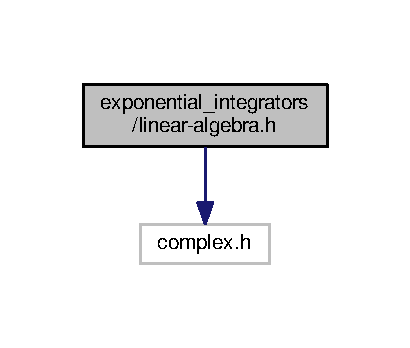
\includegraphics[width=197pt]{linear-algebra_8h__incl}
\end{center}
\end{figure}
This graph shows which files directly or indirectly include this file\+:\nopagebreak
\begin{figure}[H]
\begin{center}
\leavevmode
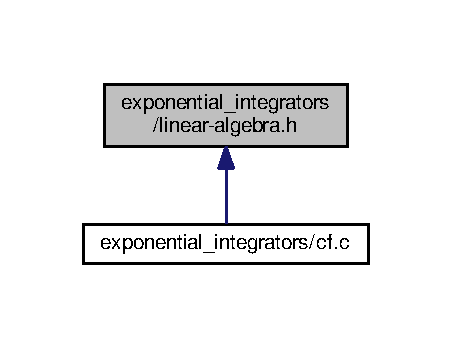
\includegraphics[width=217pt]{linear-algebra_8h__dep__incl}
\end{center}
\end{figure}
\subsection*{Functions}
\begin{DoxyCompactItemize}
\item 
void \hyperlink{linear-algebra_8h_aaad22cd21b2c37f50d56bc10e562552c}{get\+Inverse\+Complex} (int, double complex $\ast$)
\begin{DoxyCompactList}\small\item\em Interface function to L\+A\+P\+A\+CK matrix inversion subroutine. \end{DoxyCompactList}\item 
void \hyperlink{linear-algebra_8h_a3c19505e0d860542b51152f7037a6261}{lin\+Solve\+Complex} (int, double complex $\ast$, double complex $\ast$, double complex $\ast$)
\begin{DoxyCompactList}\small\item\em Solves the complex linear system Ax = B. \end{DoxyCompactList}\item 
void \hyperlink{linear-algebra_8h_aa90f025f46d234d3a36724d2d6208bea}{roots} (int, double $\ast$, double complex $\ast$)
\begin{DoxyCompactList}\small\item\em Polynomial root finding function. \end{DoxyCompactList}\item 
void \hyperlink{linear-algebra_8h_ad1c551a05773d4e45a8a4d563b2acdda}{svd} (int, double $\ast$, double $\ast$, double $\ast$, double $\ast$)
\begin{DoxyCompactList}\small\item\em Singular value decomposition function. \end{DoxyCompactList}\end{DoxyCompactItemize}


\subsection{Function Documentation}
\index{linear-\/algebra.\+h@{linear-\/algebra.\+h}!get\+Inverse\+Complex@{get\+Inverse\+Complex}}
\index{get\+Inverse\+Complex@{get\+Inverse\+Complex}!linear-\/algebra.\+h@{linear-\/algebra.\+h}}
\subsubsection[{\texorpdfstring{get\+Inverse\+Complex(int, double complex $\ast$)}{getInverseComplex(int, double complex *)}}]{\setlength{\rightskip}{0pt plus 5cm}void get\+Inverse\+Complex (
\begin{DoxyParamCaption}
\item[{int}]{n, }
\item[{double complex $\ast$}]{A}
\end{DoxyParamCaption}
)}\hypertarget{linear-algebra_8h_aaad22cd21b2c37f50d56bc10e562552c}{}\label{linear-algebra_8h_aaad22cd21b2c37f50d56bc10e562552c}


Interface function to L\+A\+P\+A\+CK matrix inversion subroutine. 

Performs inversion of square matrix. Uses L\+A\+P\+A\+CK subroutines D\+G\+E\+T\+RF and D\+G\+E\+T\+RI.


\begin{DoxyParams}[1]{Parameters}
\mbox{\tt in}  & {\em n} & order of matrix \\
\hline
\mbox{\tt in}  & {\em A} & the input matrix, size n$\ast$n \\
\hline
\end{DoxyParams}
\begin{DoxyReturn}{Returns}
info success/fail integer flag 
\end{DoxyReturn}
\index{linear-\/algebra.\+h@{linear-\/algebra.\+h}!lin\+Solve\+Complex@{lin\+Solve\+Complex}}
\index{lin\+Solve\+Complex@{lin\+Solve\+Complex}!linear-\/algebra.\+h@{linear-\/algebra.\+h}}
\subsubsection[{\texorpdfstring{lin\+Solve\+Complex(int, double complex $\ast$, double complex $\ast$, double complex $\ast$)}{linSolveComplex(int, double complex *, double complex *, double complex *)}}]{\setlength{\rightskip}{0pt plus 5cm}void lin\+Solve\+Complex (
\begin{DoxyParamCaption}
\item[{int}]{n, }
\item[{double complex $\ast$}]{A, }
\item[{double complex $\ast$}]{B, }
\item[{double complex $\ast$}]{x}
\end{DoxyParamCaption}
)}\hypertarget{linear-algebra_8h_a3c19505e0d860542b51152f7037a6261}{}\label{linear-algebra_8h_a3c19505e0d860542b51152f7037a6261}


Solves the complex linear system Ax = B. 

Performs inversion of square matrix. Uses L\+A\+P\+A\+CK subroutines D\+G\+E\+T\+RF and D\+G\+E\+T\+RI.


\begin{DoxyParams}[1]{Parameters}
\mbox{\tt in}  & {\em n} & order of matrix \\
\hline
\mbox{\tt in}  & {\em A} & the L\+HS matrix, size n$\ast$n \\
\hline
\mbox{\tt in}  & {\em B} & the R\+HS matrix, size n$\ast$n \\
\hline
\mbox{\tt out}  & {\em x} & the solved vector, size n$\ast$1 \\
\hline
\end{DoxyParams}
\index{linear-\/algebra.\+h@{linear-\/algebra.\+h}!roots@{roots}}
\index{roots@{roots}!linear-\/algebra.\+h@{linear-\/algebra.\+h}}
\subsubsection[{\texorpdfstring{roots(int, double $\ast$, double complex $\ast$)}{roots(int, double *, double complex *)}}]{\setlength{\rightskip}{0pt plus 5cm}void roots (
\begin{DoxyParamCaption}
\item[{int}]{n, }
\item[{double $\ast$}]{v, }
\item[{double complex $\ast$}]{rt}
\end{DoxyParamCaption}
)}\hypertarget{linear-algebra_8h_aa90f025f46d234d3a36724d2d6208bea}{}\label{linear-algebra_8h_aa90f025f46d234d3a36724d2d6208bea}


Polynomial root finding function. 

This function calculates the roots of a polynomial represented by its coefficients in the array v. This is done by constructing a companion matrix out of the polynomial coefficients, then using the L\+A\+P\+A\+CK subroutine D\+G\+E\+EV to calculate its eigenvalues. These are the roots of the polynomial.


\begin{DoxyParams}[1]{Parameters}
\mbox{\tt in}  & {\em n} & size of v; \\
\hline
\mbox{\tt in}  & {\em v} & array of polynomial coefficients (real) \\
\hline
\mbox{\tt out}  & {\em rt} & array of polynomial roots (complex), size n -\/ 1 \\
\hline
\end{DoxyParams}
\index{linear-\/algebra.\+h@{linear-\/algebra.\+h}!svd@{svd}}
\index{svd@{svd}!linear-\/algebra.\+h@{linear-\/algebra.\+h}}
\subsubsection[{\texorpdfstring{svd(int, double $\ast$, double $\ast$, double $\ast$, double $\ast$)}{svd(int, double *, double *, double *, double *)}}]{\setlength{\rightskip}{0pt plus 5cm}void svd (
\begin{DoxyParamCaption}
\item[{int}]{n, }
\item[{double $\ast$}]{A, }
\item[{double $\ast$}]{S, }
\item[{double $\ast$}]{U, }
\item[{double $\ast$}]{V}
\end{DoxyParamCaption}
)}\hypertarget{linear-algebra_8h_ad1c551a05773d4e45a8a4d563b2acdda}{}\label{linear-algebra_8h_ad1c551a05773d4e45a8a4d563b2acdda}


Singular value decomposition function. 

Decomposes a matrix A into U $\ast$ S $\ast$ V\textquotesingle{}, where S (here an array, really a diagonal matrix) holds the singular values. The function uses the L\+A\+P\+A\+CK subroutine D\+G\+E\+S\+VD.


\begin{DoxyParams}[1]{Parameters}
\mbox{\tt in}  & {\em n} & leading dimension of array \\
\hline
\mbox{\tt in}  & {\em A} & array to be decomposed, size n $\ast$ n \\
\hline
\mbox{\tt out}  & {\em S} & array with singular values, size n \\
\hline
\mbox{\tt out}  & {\em U} & array with left singular vectors, size n $\ast$ n \\
\hline
\mbox{\tt out}  & {\em V} & array with right singular vectors, size n $\ast$ n \\
\hline
\end{DoxyParams}

\hypertarget{phiAHessenberg_8c}{}\section{/home/nick/\+Dropbox/acceler\+Int/exponential\+\_\+integrators/phi\+A\+Hessenberg.c File Reference}
\label{phiAHessenberg_8c}\index{/home/nick/\+Dropbox/acceler\+Int/exponential\+\_\+integrators/phi\+A\+Hessenberg.\+c@{/home/nick/\+Dropbox/acceler\+Int/exponential\+\_\+integrators/phi\+A\+Hessenberg.\+c}}


Computes various matrix exponential functions on the Krylov Hessenberg matricies.  


{\ttfamily \#include $<$stdlib.\+h$>$}\\*
{\ttfamily \#include $<$complex.\+h$>$}\\*
{\ttfamily \#include \char`\"{}header.\+h\char`\"{}}\\*
{\ttfamily \#include \char`\"{}lapack\+\_\+dfns.\+h\char`\"{}}\\*
{\ttfamily \#include \char`\"{}complex\+Inverse.\+h\char`\"{}}\\*
{\ttfamily \#include \char`\"{}solver\+\_\+options.\+h\char`\"{}}\\*
{\ttfamily \#include \char`\"{}solver\+\_\+props.\+h\char`\"{}}\\*
Include dependency graph for phi\+A\+Hessenberg.\+c\+:
\nopagebreak
\begin{figure}[H]
\begin{center}
\leavevmode
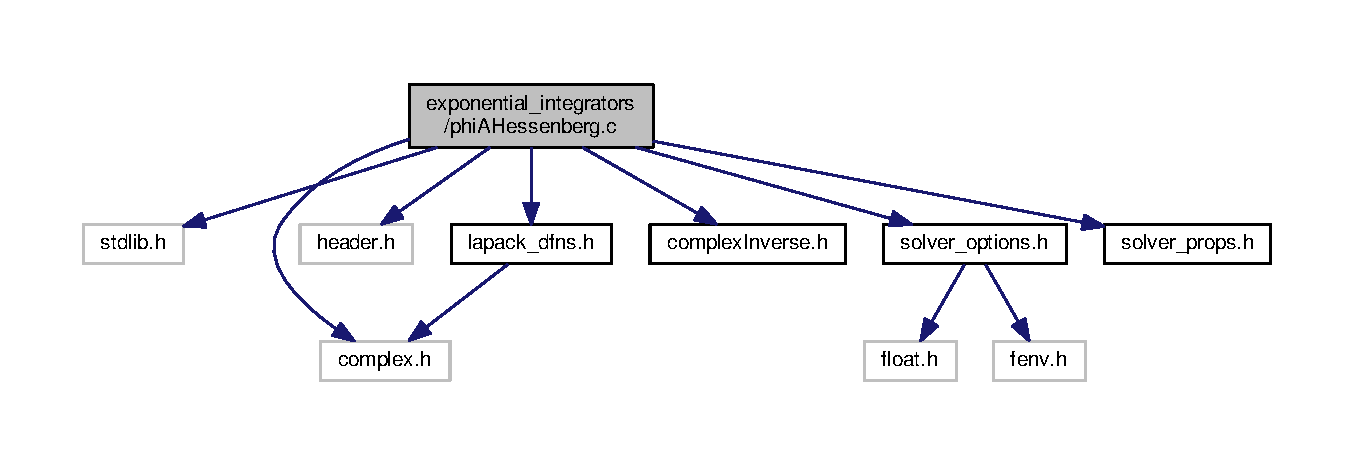
\includegraphics[width=350pt]{phiAHessenberg_8c__incl}
\end{center}
\end{figure}
\subsection*{Functions}
\begin{DoxyCompactItemize}
\item 
int \hyperlink{phiAHessenberg_8c_a325b6ad1fdc0c8b7034850650476d2a8}{phi2\+Ac\+\_\+variable} (const int m, const double $\ast$A, const double c, double $\ast$phiA)
\begin{DoxyCompactList}\small\item\em Compute the 2nd order Phi (exponential) matrix function. \end{DoxyCompactList}\item 
int \hyperlink{phiAHessenberg_8c_a57e61ff53c0c0488f9ad95c73498211b}{phi\+Ac\+\_\+variable} (const int m, const double $\ast$A, const double c, double $\ast$phiA)
\begin{DoxyCompactList}\small\item\em Compute the first order Phi (exponential) matrix function. \end{DoxyCompactList}\item 
int \hyperlink{phiAHessenberg_8c_a40fdec1db4c10f21dc027b03a908700a}{exp\+Ac\+\_\+variable} (const int m, const double $\ast$A, const double c, double $\ast$phiA)
\begin{DoxyCompactList}\small\item\em Compute the zeroth order Phi (exponential) matrix function. This is the regular matrix exponential. \end{DoxyCompactList}\end{DoxyCompactItemize}
\subsection*{Variables}
\begin{DoxyCompactItemize}
\item 
double complex \hyperlink{phiAHessenberg_8c_a48b61efd6d33096c7c1b014f817d1baf}{poles} \mbox{[}\hyperlink{solver__options_8h_a69f5533c684b73d07a7e20146a285cb1}{N\+\_\+\+RA}\mbox{]}
\item 
double complex \hyperlink{phiAHessenberg_8c_a2df94bdd03b8eb32a977adec203dadef}{res} \mbox{[}\hyperlink{solver__options_8h_a69f5533c684b73d07a7e20146a285cb1}{N\+\_\+\+RA}\mbox{]}
\end{DoxyCompactItemize}


\subsection{Detailed Description}
Computes various matrix exponential functions on the Krylov Hessenberg matricies. 



\subsection{Function Documentation}
\index{phi\+A\+Hessenberg.\+c@{phi\+A\+Hessenberg.\+c}!exp\+Ac\+\_\+variable@{exp\+Ac\+\_\+variable}}
\index{exp\+Ac\+\_\+variable@{exp\+Ac\+\_\+variable}!phi\+A\+Hessenberg.\+c@{phi\+A\+Hessenberg.\+c}}
\subsubsection[{\texorpdfstring{exp\+Ac\+\_\+variable(const int m, const double $\ast$\+A, const double c, double $\ast$phi\+A)}{expAc_variable(const int m, const double *A, const double c, double *phiA)}}]{\setlength{\rightskip}{0pt plus 5cm}int exp\+Ac\+\_\+variable (
\begin{DoxyParamCaption}
\item[{const int}]{m, }
\item[{const double $\ast$}]{A, }
\item[{const double}]{c, }
\item[{double $\ast$}]{phiA}
\end{DoxyParamCaption}
)}\hypertarget{phiAHessenberg_8c_a40fdec1db4c10f21dc027b03a908700a}{}\label{phiAHessenberg_8c_a40fdec1db4c10f21dc027b03a908700a}


Compute the zeroth order Phi (exponential) matrix function. This is the regular matrix exponential. 

Computes $\phi_0(c*A)$


\begin{DoxyParams}[1]{Parameters}
\mbox{\tt in}  & {\em m} & The Hessenberg matrix size (mxm) \\
\hline
\mbox{\tt in}  & {\em A} & The input Hessenberg matrix \\
\hline
\mbox{\tt in}  & {\em c} & The scaling factor \\
\hline
\mbox{\tt out}  & {\em phiA} & The resulting exponential matrix \\
\hline
\end{DoxyParams}
\index{phi\+A\+Hessenberg.\+c@{phi\+A\+Hessenberg.\+c}!phi2\+Ac\+\_\+variable@{phi2\+Ac\+\_\+variable}}
\index{phi2\+Ac\+\_\+variable@{phi2\+Ac\+\_\+variable}!phi\+A\+Hessenberg.\+c@{phi\+A\+Hessenberg.\+c}}
\subsubsection[{\texorpdfstring{phi2\+Ac\+\_\+variable(const int m, const double $\ast$\+A, const double c, double $\ast$phi\+A)}{phi2Ac_variable(const int m, const double *A, const double c, double *phiA)}}]{\setlength{\rightskip}{0pt plus 5cm}int phi2\+Ac\+\_\+variable (
\begin{DoxyParamCaption}
\item[{const int}]{m, }
\item[{const double $\ast$}]{A, }
\item[{const double}]{c, }
\item[{double $\ast$}]{phiA}
\end{DoxyParamCaption}
)}\hypertarget{phiAHessenberg_8c_a325b6ad1fdc0c8b7034850650476d2a8}{}\label{phiAHessenberg_8c_a325b6ad1fdc0c8b7034850650476d2a8}


Compute the 2nd order Phi (exponential) matrix function. 

Computes $\phi_2(c*A)$


\begin{DoxyParams}[1]{Parameters}
\mbox{\tt in}  & {\em m} & The Hessenberg matrix size (mxm) \\
\hline
\mbox{\tt in}  & {\em A} & The input Hessenberg matrix \\
\hline
\mbox{\tt in}  & {\em c} & The scaling factor \\
\hline
\mbox{\tt out}  & {\em phiA} & The resulting exponential matrix \\
\hline
\end{DoxyParams}
\index{phi\+A\+Hessenberg.\+c@{phi\+A\+Hessenberg.\+c}!phi\+Ac\+\_\+variable@{phi\+Ac\+\_\+variable}}
\index{phi\+Ac\+\_\+variable@{phi\+Ac\+\_\+variable}!phi\+A\+Hessenberg.\+c@{phi\+A\+Hessenberg.\+c}}
\subsubsection[{\texorpdfstring{phi\+Ac\+\_\+variable(const int m, const double $\ast$\+A, const double c, double $\ast$phi\+A)}{phiAc_variable(const int m, const double *A, const double c, double *phiA)}}]{\setlength{\rightskip}{0pt plus 5cm}int phi\+Ac\+\_\+variable (
\begin{DoxyParamCaption}
\item[{const int}]{m, }
\item[{const double $\ast$}]{A, }
\item[{const double}]{c, }
\item[{double $\ast$}]{phiA}
\end{DoxyParamCaption}
)}\hypertarget{phiAHessenberg_8c_a57e61ff53c0c0488f9ad95c73498211b}{}\label{phiAHessenberg_8c_a57e61ff53c0c0488f9ad95c73498211b}


Compute the first order Phi (exponential) matrix function. 

Computes $\phi_1(c*A)$


\begin{DoxyParams}[1]{Parameters}
\mbox{\tt in}  & {\em m} & The Hessenberg matrix size (mxm) \\
\hline
\mbox{\tt in}  & {\em A} & The input Hessenberg matrix \\
\hline
\mbox{\tt in}  & {\em c} & The scaling factor \\
\hline
\mbox{\tt out}  & {\em phiA} & The resulting exponential matrix \\
\hline
\end{DoxyParams}


\subsection{Variable Documentation}
\index{phi\+A\+Hessenberg.\+c@{phi\+A\+Hessenberg.\+c}!poles@{poles}}
\index{poles@{poles}!phi\+A\+Hessenberg.\+c@{phi\+A\+Hessenberg.\+c}}
\subsubsection[{\texorpdfstring{poles}{poles}}]{\setlength{\rightskip}{0pt plus 5cm}double complex poles\mbox{[}{\bf N\+\_\+\+RA}\mbox{]}}\hypertarget{phiAHessenberg_8c_a48b61efd6d33096c7c1b014f817d1baf}{}\label{phiAHessenberg_8c_a48b61efd6d33096c7c1b014f817d1baf}
\index{phi\+A\+Hessenberg.\+c@{phi\+A\+Hessenberg.\+c}!res@{res}}
\index{res@{res}!phi\+A\+Hessenberg.\+c@{phi\+A\+Hessenberg.\+c}}
\subsubsection[{\texorpdfstring{res}{res}}]{\setlength{\rightskip}{0pt plus 5cm}double complex res\mbox{[}{\bf N\+\_\+\+RA}\mbox{]}}\hypertarget{phiAHessenberg_8c_a2df94bdd03b8eb32a977adec203dadef}{}\label{phiAHessenberg_8c_a2df94bdd03b8eb32a977adec203dadef}

\hypertarget{phiAHessenberg_8cu}{}\section{exponential\+\_\+integrators/phi\+A\+Hessenberg.cu File Reference}
\label{phiAHessenberg_8cu}\index{exponential\+\_\+integrators/phi\+A\+Hessenberg.\+cu@{exponential\+\_\+integrators/phi\+A\+Hessenberg.\+cu}}


Computes various matrix exponential functions on the Krylov Hessenberg matricies.  


{\ttfamily \#include $<$stdlib.\+h$>$}\\*
{\ttfamily \#include \char`\"{}header.\+cuh\char`\"{}}\\*
{\ttfamily \#include \char`\"{}solver\+\_\+options.\+cuh\char`\"{}}\\*
{\ttfamily \#include \char`\"{}solver\+\_\+props.\+cuh\char`\"{}}\\*
{\ttfamily \#include \char`\"{}complex\+Inverse.\+cuh\char`\"{}}\\*
Include dependency graph for phi\+A\+Hessenberg.\+cu\+:\nopagebreak
\begin{figure}[H]
\begin{center}
\leavevmode
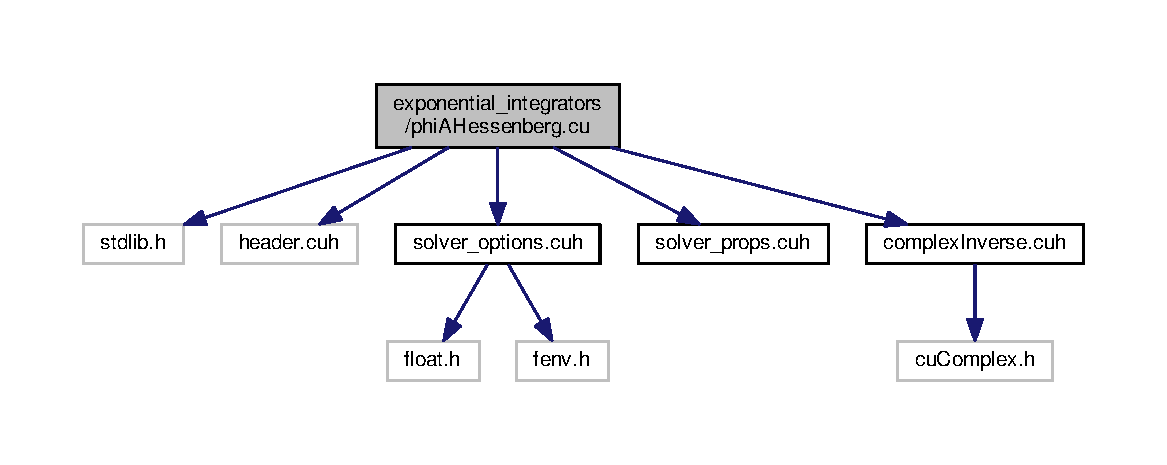
\includegraphics[width=350pt]{phiAHessenberg_8cu__incl}
\end{center}
\end{figure}
\subsection*{Functions}
\begin{DoxyCompactItemize}
\item 
\+\_\+\+\_\+device\+\_\+\+\_\+ int \hyperlink{phiAHessenberg_8cu_ae7972d89009078777211b58162f2dd76}{phi2\+Ac\+\_\+variable} (const int m, const double $\ast$\+\_\+\+\_\+restrict\+\_\+\+\_\+ A, const double c, double $\ast$\+\_\+\+\_\+restrict\+\_\+\+\_\+ phiA, const \hyperlink{structsolver__memory}{solver\+\_\+memory} $\ast$\+\_\+\+\_\+restrict\+\_\+\+\_\+ solver, cu\+Double\+Complex $\ast$\+\_\+\+\_\+restrict\+\_\+\+\_\+ work)
\begin{DoxyCompactList}\small\item\em Compute the 2nd order Phi (exponential) matrix function. \end{DoxyCompactList}\item 
\+\_\+\+\_\+device\+\_\+\+\_\+ int \hyperlink{phiAHessenberg_8cu_abbb130c60c0fdda920f46468175a7904}{phi\+Ac\+\_\+variable} (const int m, const double $\ast$\+\_\+\+\_\+restrict\+\_\+\+\_\+ A, const double c, double $\ast$\+\_\+\+\_\+restrict\+\_\+\+\_\+ phiA, const \hyperlink{structsolver__memory}{solver\+\_\+memory} $\ast$\+\_\+\+\_\+restrict\+\_\+\+\_\+ solver, cu\+Double\+Complex $\ast$\+\_\+\+\_\+restrict\+\_\+\+\_\+ work)
\begin{DoxyCompactList}\small\item\em Compute the first order Phi (exponential) matrix function. \end{DoxyCompactList}\item 
\+\_\+\+\_\+device\+\_\+\+\_\+ int \hyperlink{phiAHessenberg_8cu_acf9f2fca33bcd8e9729601ed3761292a}{exp\+Ac\+\_\+variable} (const int m, const double $\ast$\+\_\+\+\_\+restrict\+\_\+\+\_\+ A, const double c, double $\ast$\+\_\+\+\_\+restrict\+\_\+\+\_\+ phiA, const \hyperlink{structsolver__memory}{solver\+\_\+memory} $\ast$\+\_\+\+\_\+restrict\+\_\+\+\_\+ solver, cu\+Double\+Complex $\ast$\+\_\+\+\_\+restrict\+\_\+\+\_\+ work)
\begin{DoxyCompactList}\small\item\em Compute the zeroth order Phi (exponential) matrix function. This is the regular matrix exponential. \end{DoxyCompactList}\end{DoxyCompactItemize}
\subsection*{Variables}
\begin{DoxyCompactItemize}
\item 
\+\_\+\+\_\+device\+\_\+\+\_\+ \+\_\+\+\_\+constant\+\_\+\+\_\+ cu\+Double\+Complex \hyperlink{phiAHessenberg_8cu_a4a123ce887b4a39c29859b77db90e7e2}{poles} \mbox{[}\hyperlink{solver__options_8h_a69f5533c684b73d07a7e20146a285cb1}{N\+\_\+\+RA}\mbox{]}
\item 
\+\_\+\+\_\+device\+\_\+\+\_\+ \+\_\+\+\_\+constant\+\_\+\+\_\+ cu\+Double\+Complex \hyperlink{phiAHessenberg_8cu_af309432c3d053cc809c36518fb7d7f00}{res} \mbox{[}\hyperlink{solver__options_8h_a69f5533c684b73d07a7e20146a285cb1}{N\+\_\+\+RA}\mbox{]}
\end{DoxyCompactItemize}


\subsection{Detailed Description}
Computes various matrix exponential functions on the Krylov Hessenberg matricies. 



\subsection{Function Documentation}
\index{phi\+A\+Hessenberg.\+cu@{phi\+A\+Hessenberg.\+cu}!exp\+Ac\+\_\+variable@{exp\+Ac\+\_\+variable}}
\index{exp\+Ac\+\_\+variable@{exp\+Ac\+\_\+variable}!phi\+A\+Hessenberg.\+cu@{phi\+A\+Hessenberg.\+cu}}
\subsubsection[{\texorpdfstring{exp\+Ac\+\_\+variable(const int m, const double $\ast$\+\_\+\+\_\+restrict\+\_\+\+\_\+ A, const double c, double $\ast$\+\_\+\+\_\+restrict\+\_\+\+\_\+ phi\+A, const solver\+\_\+memory $\ast$\+\_\+\+\_\+restrict\+\_\+\+\_\+ solver, cu\+Double\+Complex $\ast$\+\_\+\+\_\+restrict\+\_\+\+\_\+ work)}{expAc_variable(const int m, const double *__restrict__ A, const double c, double *__restrict__ phiA, const solver_memory *__restrict__ solver, cuDoubleComplex *__restrict__ work)}}]{\setlength{\rightskip}{0pt plus 5cm}\+\_\+\+\_\+device\+\_\+\+\_\+ int exp\+Ac\+\_\+variable (
\begin{DoxyParamCaption}
\item[{const int}]{m, }
\item[{const double $\ast$\+\_\+\+\_\+restrict\+\_\+\+\_\+}]{A, }
\item[{const double}]{c, }
\item[{double $\ast$\+\_\+\+\_\+restrict\+\_\+\+\_\+}]{phiA, }
\item[{const {\bf solver\+\_\+memory} $\ast$\+\_\+\+\_\+restrict\+\_\+\+\_\+}]{solver, }
\item[{cu\+Double\+Complex $\ast$\+\_\+\+\_\+restrict\+\_\+\+\_\+}]{work}
\end{DoxyParamCaption}
)}\hypertarget{phiAHessenberg_8cu_acf9f2fca33bcd8e9729601ed3761292a}{}\label{phiAHessenberg_8cu_acf9f2fca33bcd8e9729601ed3761292a}


Compute the zeroth order Phi (exponential) matrix function. This is the regular matrix exponential. 

Computes $\phi_0(c*A)$


\begin{DoxyParams}[1]{Parameters}
\mbox{\tt in}  & {\em m} & The Hessenberg matrix size (mxm) \\
\hline
\mbox{\tt in}  & {\em A} & The input Hessenberg matrix \\
\hline
\mbox{\tt in}  & {\em c} & The scaling factor \\
\hline
\mbox{\tt out}  & {\em phiA} & The resulting exponential matrix \\
\hline
\mbox{\tt in}  & {\em solver} & The \hyperlink{structsolver__memory}{solver\+\_\+memory} object \\
\hline
\mbox{\tt in}  & {\em work} & A complex work array \\
\hline
\end{DoxyParams}
\index{phi\+A\+Hessenberg.\+cu@{phi\+A\+Hessenberg.\+cu}!phi2\+Ac\+\_\+variable@{phi2\+Ac\+\_\+variable}}
\index{phi2\+Ac\+\_\+variable@{phi2\+Ac\+\_\+variable}!phi\+A\+Hessenberg.\+cu@{phi\+A\+Hessenberg.\+cu}}
\subsubsection[{\texorpdfstring{phi2\+Ac\+\_\+variable(const int m, const double $\ast$\+\_\+\+\_\+restrict\+\_\+\+\_\+ A, const double c, double $\ast$\+\_\+\+\_\+restrict\+\_\+\+\_\+ phi\+A, const solver\+\_\+memory $\ast$\+\_\+\+\_\+restrict\+\_\+\+\_\+ solver, cu\+Double\+Complex $\ast$\+\_\+\+\_\+restrict\+\_\+\+\_\+ work)}{phi2Ac_variable(const int m, const double *__restrict__ A, const double c, double *__restrict__ phiA, const solver_memory *__restrict__ solver, cuDoubleComplex *__restrict__ work)}}]{\setlength{\rightskip}{0pt plus 5cm}\+\_\+\+\_\+device\+\_\+\+\_\+ int phi2\+Ac\+\_\+variable (
\begin{DoxyParamCaption}
\item[{const int}]{m, }
\item[{const double $\ast$\+\_\+\+\_\+restrict\+\_\+\+\_\+}]{A, }
\item[{const double}]{c, }
\item[{double $\ast$\+\_\+\+\_\+restrict\+\_\+\+\_\+}]{phiA, }
\item[{const {\bf solver\+\_\+memory} $\ast$\+\_\+\+\_\+restrict\+\_\+\+\_\+}]{solver, }
\item[{cu\+Double\+Complex $\ast$\+\_\+\+\_\+restrict\+\_\+\+\_\+}]{work}
\end{DoxyParamCaption}
)}\hypertarget{phiAHessenberg_8cu_ae7972d89009078777211b58162f2dd76}{}\label{phiAHessenberg_8cu_ae7972d89009078777211b58162f2dd76}


Compute the 2nd order Phi (exponential) matrix function. 

Computes $\phi_2(c*A)$


\begin{DoxyParams}[1]{Parameters}
\mbox{\tt in}  & {\em m} & The Hessenberg matrix size (mxm) \\
\hline
\mbox{\tt in}  & {\em A} & The input Hessenberg matrix \\
\hline
\mbox{\tt in}  & {\em c} & The scaling factor \\
\hline
\mbox{\tt out}  & {\em phiA} & The resulting exponential matrix \\
\hline
\mbox{\tt in}  & {\em solver} & The \hyperlink{structsolver__memory}{solver\+\_\+memory} object \\
\hline
\mbox{\tt in}  & {\em work} & A complex work array \\
\hline
\end{DoxyParams}
\index{phi\+A\+Hessenberg.\+cu@{phi\+A\+Hessenberg.\+cu}!phi\+Ac\+\_\+variable@{phi\+Ac\+\_\+variable}}
\index{phi\+Ac\+\_\+variable@{phi\+Ac\+\_\+variable}!phi\+A\+Hessenberg.\+cu@{phi\+A\+Hessenberg.\+cu}}
\subsubsection[{\texorpdfstring{phi\+Ac\+\_\+variable(const int m, const double $\ast$\+\_\+\+\_\+restrict\+\_\+\+\_\+ A, const double c, double $\ast$\+\_\+\+\_\+restrict\+\_\+\+\_\+ phi\+A, const solver\+\_\+memory $\ast$\+\_\+\+\_\+restrict\+\_\+\+\_\+ solver, cu\+Double\+Complex $\ast$\+\_\+\+\_\+restrict\+\_\+\+\_\+ work)}{phiAc_variable(const int m, const double *__restrict__ A, const double c, double *__restrict__ phiA, const solver_memory *__restrict__ solver, cuDoubleComplex *__restrict__ work)}}]{\setlength{\rightskip}{0pt plus 5cm}\+\_\+\+\_\+device\+\_\+\+\_\+ int phi\+Ac\+\_\+variable (
\begin{DoxyParamCaption}
\item[{const int}]{m, }
\item[{const double $\ast$\+\_\+\+\_\+restrict\+\_\+\+\_\+}]{A, }
\item[{const double}]{c, }
\item[{double $\ast$\+\_\+\+\_\+restrict\+\_\+\+\_\+}]{phiA, }
\item[{const {\bf solver\+\_\+memory} $\ast$\+\_\+\+\_\+restrict\+\_\+\+\_\+}]{solver, }
\item[{cu\+Double\+Complex $\ast$\+\_\+\+\_\+restrict\+\_\+\+\_\+}]{work}
\end{DoxyParamCaption}
)}\hypertarget{phiAHessenberg_8cu_abbb130c60c0fdda920f46468175a7904}{}\label{phiAHessenberg_8cu_abbb130c60c0fdda920f46468175a7904}


Compute the first order Phi (exponential) matrix function. 

Computes $\phi_1(c*A)$


\begin{DoxyParams}[1]{Parameters}
\mbox{\tt in}  & {\em m} & The Hessenberg matrix size (mxm) \\
\hline
\mbox{\tt in}  & {\em A} & The input Hessenberg matrix \\
\hline
\mbox{\tt in}  & {\em c} & The scaling factor \\
\hline
\mbox{\tt out}  & {\em phiA} & The resulting exponential matrix \\
\hline
\mbox{\tt in}  & {\em solver} & The \hyperlink{structsolver__memory}{solver\+\_\+memory} object \\
\hline
\mbox{\tt in}  & {\em work} & A complex work array \\
\hline
\end{DoxyParams}


\subsection{Variable Documentation}
\index{phi\+A\+Hessenberg.\+cu@{phi\+A\+Hessenberg.\+cu}!poles@{poles}}
\index{poles@{poles}!phi\+A\+Hessenberg.\+cu@{phi\+A\+Hessenberg.\+cu}}
\subsubsection[{\texorpdfstring{poles}{poles}}]{\setlength{\rightskip}{0pt plus 5cm}\+\_\+\+\_\+device\+\_\+\+\_\+ \+\_\+\+\_\+constant\+\_\+\+\_\+ cu\+Double\+Complex poles\mbox{[}{\bf N\+\_\+\+RA}\mbox{]}}\hypertarget{phiAHessenberg_8cu_a4a123ce887b4a39c29859b77db90e7e2}{}\label{phiAHessenberg_8cu_a4a123ce887b4a39c29859b77db90e7e2}
\index{phi\+A\+Hessenberg.\+cu@{phi\+A\+Hessenberg.\+cu}!res@{res}}
\index{res@{res}!phi\+A\+Hessenberg.\+cu@{phi\+A\+Hessenberg.\+cu}}
\subsubsection[{\texorpdfstring{res}{res}}]{\setlength{\rightskip}{0pt plus 5cm}\+\_\+\+\_\+device\+\_\+\+\_\+ \+\_\+\+\_\+constant\+\_\+\+\_\+ cu\+Double\+Complex res\mbox{[}{\bf N\+\_\+\+RA}\mbox{]}}\hypertarget{phiAHessenberg_8cu_af309432c3d053cc809c36518fb7d7f00}{}\label{phiAHessenberg_8cu_af309432c3d053cc809c36518fb7d7f00}

\hypertarget{phiAHessenberg_8cuh}{}\section{exponential\+\_\+integrators/phi\+A\+Hessenberg.cuh File Reference}
\label{phiAHessenberg_8cuh}\index{exponential\+\_\+integrators/phi\+A\+Hessenberg.\+cuh@{exponential\+\_\+integrators/phi\+A\+Hessenberg.\+cuh}}
{\ttfamily \#include \char`\"{}header.\+cuh\char`\"{}}\\*
Include dependency graph for phi\+A\+Hessenberg.\+cuh\+:\nopagebreak
\begin{figure}[H]
\begin{center}
\leavevmode
\includegraphics[width=197pt]{phiAHessenberg_8cuh__incl}
\end{center}
\end{figure}
This graph shows which files directly or indirectly include this file\+:\nopagebreak
\begin{figure}[H]
\begin{center}
\leavevmode
\includegraphics[width=332pt]{phiAHessenberg_8cuh__dep__incl}
\end{center}
\end{figure}
\subsection*{Macros}
\begin{DoxyCompactItemize}
\item 
\#define \hyperlink{phiAHessenberg_8cuh_a3cd1f20586504db36f26cc1dbe605dc1}{P\+H\+I\+A\+\_\+\+H\+E\+A\+D\+\_\+\+H\+E\+S\+S\+E\+N\+B\+E\+R\+G\+\_\+\+CU}
\end{DoxyCompactItemize}
\subsection*{Functions}
\begin{DoxyCompactItemize}
\item 
\+\_\+\+\_\+device\+\_\+\+\_\+ int \hyperlink{phiAHessenberg_8cuh_a6daaee3ff7b872cd3bf32bdfda84b68a}{phi2\+Ac\+\_\+variable} (const int, const double $\ast$\+\_\+\+\_\+restrict\+\_\+\+\_\+, const double, double $\ast$\+\_\+\+\_\+restrict\+\_\+\+\_\+, const \hyperlink{structsolver__memory}{solver\+\_\+memory} $\ast$\+\_\+\+\_\+restrict\+\_\+\+\_\+, cu\+Double\+Complex $\ast$\+\_\+\+\_\+restrict\+\_\+\+\_\+)
\item 
\+\_\+\+\_\+device\+\_\+\+\_\+ int \hyperlink{phiAHessenberg_8cuh_aa917e9051a8f04b5d7643b27e8367688}{phi\+Ac\+\_\+variable} (const int, const double $\ast$\+\_\+\+\_\+restrict\+\_\+\+\_\+, const double, double $\ast$\+\_\+\+\_\+restrict\+\_\+\+\_\+, const \hyperlink{structsolver__memory}{solver\+\_\+memory} $\ast$\+\_\+\+\_\+restrict\+\_\+\+\_\+, cu\+Double\+Complex $\ast$\+\_\+\+\_\+restrict\+\_\+\+\_\+)
\item 
\+\_\+\+\_\+device\+\_\+\+\_\+ int \hyperlink{phiAHessenberg_8cuh_ab94b849aefe94d752806790b9788247d}{exp\+Ac\+\_\+variable} (const int, const double $\ast$\+\_\+\+\_\+restrict\+\_\+\+\_\+, const double, double $\ast$\+\_\+\+\_\+restrict\+\_\+\+\_\+, const \hyperlink{structsolver__memory}{solver\+\_\+memory} $\ast$\+\_\+\+\_\+restrict\+\_\+\+\_\+, cu\+Double\+Complex $\ast$\+\_\+\+\_\+restrict\+\_\+\+\_\+)
\end{DoxyCompactItemize}


\subsection{Macro Definition Documentation}
\index{phi\+A\+Hessenberg.\+cuh@{phi\+A\+Hessenberg.\+cuh}!P\+H\+I\+A\+\_\+\+H\+E\+A\+D\+\_\+\+H\+E\+S\+S\+E\+N\+B\+E\+R\+G\+\_\+\+CU@{P\+H\+I\+A\+\_\+\+H\+E\+A\+D\+\_\+\+H\+E\+S\+S\+E\+N\+B\+E\+R\+G\+\_\+\+CU}}
\index{P\+H\+I\+A\+\_\+\+H\+E\+A\+D\+\_\+\+H\+E\+S\+S\+E\+N\+B\+E\+R\+G\+\_\+\+CU@{P\+H\+I\+A\+\_\+\+H\+E\+A\+D\+\_\+\+H\+E\+S\+S\+E\+N\+B\+E\+R\+G\+\_\+\+CU}!phi\+A\+Hessenberg.\+cuh@{phi\+A\+Hessenberg.\+cuh}}
\subsubsection[{\texorpdfstring{P\+H\+I\+A\+\_\+\+H\+E\+A\+D\+\_\+\+H\+E\+S\+S\+E\+N\+B\+E\+R\+G\+\_\+\+CU}{PHIA_HEAD_HESSENBERG_CU}}]{\setlength{\rightskip}{0pt plus 5cm}\#define P\+H\+I\+A\+\_\+\+H\+E\+A\+D\+\_\+\+H\+E\+S\+S\+E\+N\+B\+E\+R\+G\+\_\+\+CU}\hypertarget{phiAHessenberg_8cuh_a3cd1f20586504db36f26cc1dbe605dc1}{}\label{phiAHessenberg_8cuh_a3cd1f20586504db36f26cc1dbe605dc1}


\subsection{Function Documentation}
\index{phi\+A\+Hessenberg.\+cuh@{phi\+A\+Hessenberg.\+cuh}!exp\+Ac\+\_\+variable@{exp\+Ac\+\_\+variable}}
\index{exp\+Ac\+\_\+variable@{exp\+Ac\+\_\+variable}!phi\+A\+Hessenberg.\+cuh@{phi\+A\+Hessenberg.\+cuh}}
\subsubsection[{\texorpdfstring{exp\+Ac\+\_\+variable(const int, const double $\ast$\+\_\+\+\_\+restrict\+\_\+\+\_\+, const double, double $\ast$\+\_\+\+\_\+restrict\+\_\+\+\_\+, const solver\+\_\+memory $\ast$\+\_\+\+\_\+restrict\+\_\+\+\_\+, cu\+Double\+Complex $\ast$\+\_\+\+\_\+restrict\+\_\+\+\_\+)}{expAc_variable(const int, const double *__restrict__, const double, double *__restrict__, const solver_memory *__restrict__, cuDoubleComplex *__restrict__)}}]{\setlength{\rightskip}{0pt plus 5cm}\+\_\+\+\_\+device\+\_\+\+\_\+ int exp\+Ac\+\_\+variable (
\begin{DoxyParamCaption}
\item[{const int}]{, }
\item[{const double $\ast$}]{\+\_\+\+\_\+restrict\+\_\+\+\_\+, }
\item[{const double}]{, }
\item[{double $\ast$}]{\+\_\+\+\_\+restrict\+\_\+\+\_\+, }
\item[{const {\bf solver\+\_\+memory} $\ast$}]{\+\_\+\+\_\+restrict\+\_\+\+\_\+, }
\item[{cu\+Double\+Complex $\ast$}]{\+\_\+\+\_\+restrict\+\_\+\+\_\+}
\end{DoxyParamCaption}
)}\hypertarget{phiAHessenberg_8cuh_ab94b849aefe94d752806790b9788247d}{}\label{phiAHessenberg_8cuh_ab94b849aefe94d752806790b9788247d}
\index{phi\+A\+Hessenberg.\+cuh@{phi\+A\+Hessenberg.\+cuh}!phi2\+Ac\+\_\+variable@{phi2\+Ac\+\_\+variable}}
\index{phi2\+Ac\+\_\+variable@{phi2\+Ac\+\_\+variable}!phi\+A\+Hessenberg.\+cuh@{phi\+A\+Hessenberg.\+cuh}}
\subsubsection[{\texorpdfstring{phi2\+Ac\+\_\+variable(const int, const double $\ast$\+\_\+\+\_\+restrict\+\_\+\+\_\+, const double, double $\ast$\+\_\+\+\_\+restrict\+\_\+\+\_\+, const solver\+\_\+memory $\ast$\+\_\+\+\_\+restrict\+\_\+\+\_\+, cu\+Double\+Complex $\ast$\+\_\+\+\_\+restrict\+\_\+\+\_\+)}{phi2Ac_variable(const int, const double *__restrict__, const double, double *__restrict__, const solver_memory *__restrict__, cuDoubleComplex *__restrict__)}}]{\setlength{\rightskip}{0pt plus 5cm}\+\_\+\+\_\+device\+\_\+\+\_\+ int phi2\+Ac\+\_\+variable (
\begin{DoxyParamCaption}
\item[{const int}]{, }
\item[{const double $\ast$}]{\+\_\+\+\_\+restrict\+\_\+\+\_\+, }
\item[{const double}]{, }
\item[{double $\ast$}]{\+\_\+\+\_\+restrict\+\_\+\+\_\+, }
\item[{const {\bf solver\+\_\+memory} $\ast$}]{\+\_\+\+\_\+restrict\+\_\+\+\_\+, }
\item[{cu\+Double\+Complex $\ast$}]{\+\_\+\+\_\+restrict\+\_\+\+\_\+}
\end{DoxyParamCaption}
)}\hypertarget{phiAHessenberg_8cuh_a6daaee3ff7b872cd3bf32bdfda84b68a}{}\label{phiAHessenberg_8cuh_a6daaee3ff7b872cd3bf32bdfda84b68a}
\index{phi\+A\+Hessenberg.\+cuh@{phi\+A\+Hessenberg.\+cuh}!phi\+Ac\+\_\+variable@{phi\+Ac\+\_\+variable}}
\index{phi\+Ac\+\_\+variable@{phi\+Ac\+\_\+variable}!phi\+A\+Hessenberg.\+cuh@{phi\+A\+Hessenberg.\+cuh}}
\subsubsection[{\texorpdfstring{phi\+Ac\+\_\+variable(const int, const double $\ast$\+\_\+\+\_\+restrict\+\_\+\+\_\+, const double, double $\ast$\+\_\+\+\_\+restrict\+\_\+\+\_\+, const solver\+\_\+memory $\ast$\+\_\+\+\_\+restrict\+\_\+\+\_\+, cu\+Double\+Complex $\ast$\+\_\+\+\_\+restrict\+\_\+\+\_\+)}{phiAc_variable(const int, const double *__restrict__, const double, double *__restrict__, const solver_memory *__restrict__, cuDoubleComplex *__restrict__)}}]{\setlength{\rightskip}{0pt plus 5cm}\+\_\+\+\_\+device\+\_\+\+\_\+ int phi\+Ac\+\_\+variable (
\begin{DoxyParamCaption}
\item[{const int}]{, }
\item[{const double $\ast$}]{\+\_\+\+\_\+restrict\+\_\+\+\_\+, }
\item[{const double}]{, }
\item[{double $\ast$}]{\+\_\+\+\_\+restrict\+\_\+\+\_\+, }
\item[{const {\bf solver\+\_\+memory} $\ast$}]{\+\_\+\+\_\+restrict\+\_\+\+\_\+, }
\item[{cu\+Double\+Complex $\ast$}]{\+\_\+\+\_\+restrict\+\_\+\+\_\+}
\end{DoxyParamCaption}
)}\hypertarget{phiAHessenberg_8cuh_aa917e9051a8f04b5d7643b27e8367688}{}\label{phiAHessenberg_8cuh_aa917e9051a8f04b5d7643b27e8367688}

\hypertarget{phiAHessenberg_8h}{}\section{/home/nick/\+Dropbox/acceler\+Int/exponential\+\_\+integrators/phi\+A\+Hessenberg.h File Reference}
\label{phiAHessenberg_8h}\index{/home/nick/\+Dropbox/acceler\+Int/exponential\+\_\+integrators/phi\+A\+Hessenberg.\+h@{/home/nick/\+Dropbox/acceler\+Int/exponential\+\_\+integrators/phi\+A\+Hessenberg.\+h}}
{\ttfamily \#include \char`\"{}header.\+h\char`\"{}}\\*
Include dependency graph for phi\+A\+Hessenberg.\+h\+:
\nopagebreak
\begin{figure}[H]
\begin{center}
\leavevmode
\includegraphics[width=231pt]{phiAHessenberg_8h__incl}
\end{center}
\end{figure}
This graph shows which files directly or indirectly include this file\+:
\nopagebreak
\begin{figure}[H]
\begin{center}
\leavevmode
\includegraphics[width=350pt]{phiAHessenberg_8h__dep__incl}
\end{center}
\end{figure}
\subsection*{Functions}
\begin{DoxyCompactItemize}
\item 
int \hyperlink{phiAHessenberg_8h_a1515b373392005fc1adcacbc6201d6aa}{phi2\+Ac\+\_\+variable} (const int, const double $\ast$, const double, double $\ast$)
\begin{DoxyCompactList}\small\item\em Compute the 2nd order Phi (exponential) matrix function. \end{DoxyCompactList}\item 
int \hyperlink{phiAHessenberg_8h_a4572532ac096221f640dac604cefb82f}{phi\+Ac\+\_\+variable} (const int, const double $\ast$, const double, double $\ast$)
\begin{DoxyCompactList}\small\item\em Compute the first order Phi (exponential) matrix function. \end{DoxyCompactList}\item 
int \hyperlink{phiAHessenberg_8h_a2ff7e0b4c44197882484b7cef57b2511}{exp\+Ac\+\_\+variable} (const int, const double $\ast$, const double, double $\ast$)
\begin{DoxyCompactList}\small\item\em Compute the zeroth order Phi (exponential) matrix function. This is the regular matrix exponential. \end{DoxyCompactList}\end{DoxyCompactItemize}


\subsection{Function Documentation}
\index{phi\+A\+Hessenberg.\+h@{phi\+A\+Hessenberg.\+h}!exp\+Ac\+\_\+variable@{exp\+Ac\+\_\+variable}}
\index{exp\+Ac\+\_\+variable@{exp\+Ac\+\_\+variable}!phi\+A\+Hessenberg.\+h@{phi\+A\+Hessenberg.\+h}}
\subsubsection[{\texorpdfstring{exp\+Ac\+\_\+variable(const int, const double $\ast$, const double, double $\ast$)}{expAc_variable(const int, const double *, const double, double *)}}]{\setlength{\rightskip}{0pt plus 5cm}int exp\+Ac\+\_\+variable (
\begin{DoxyParamCaption}
\item[{const int}]{m, }
\item[{const double $\ast$}]{A, }
\item[{const double}]{c, }
\item[{double $\ast$}]{phiA}
\end{DoxyParamCaption}
)}\hypertarget{phiAHessenberg_8h_a2ff7e0b4c44197882484b7cef57b2511}{}\label{phiAHessenberg_8h_a2ff7e0b4c44197882484b7cef57b2511}


Compute the zeroth order Phi (exponential) matrix function. This is the regular matrix exponential. 

Computes $\phi_0(c*A)$


\begin{DoxyParams}[1]{Parameters}
\mbox{\tt in}  & {\em m} & The Hessenberg matrix size (mxm) \\
\hline
\mbox{\tt in}  & {\em A} & The input Hessenberg matrix \\
\hline
\mbox{\tt in}  & {\em c} & The scaling factor \\
\hline
\mbox{\tt out}  & {\em phiA} & The resulting exponential matrix \\
\hline
\end{DoxyParams}
\index{phi\+A\+Hessenberg.\+h@{phi\+A\+Hessenberg.\+h}!phi2\+Ac\+\_\+variable@{phi2\+Ac\+\_\+variable}}
\index{phi2\+Ac\+\_\+variable@{phi2\+Ac\+\_\+variable}!phi\+A\+Hessenberg.\+h@{phi\+A\+Hessenberg.\+h}}
\subsubsection[{\texorpdfstring{phi2\+Ac\+\_\+variable(const int, const double $\ast$, const double, double $\ast$)}{phi2Ac_variable(const int, const double *, const double, double *)}}]{\setlength{\rightskip}{0pt plus 5cm}int phi2\+Ac\+\_\+variable (
\begin{DoxyParamCaption}
\item[{const int}]{m, }
\item[{const double $\ast$}]{A, }
\item[{const double}]{c, }
\item[{double $\ast$}]{phiA}
\end{DoxyParamCaption}
)}\hypertarget{phiAHessenberg_8h_a1515b373392005fc1adcacbc6201d6aa}{}\label{phiAHessenberg_8h_a1515b373392005fc1adcacbc6201d6aa}


Compute the 2nd order Phi (exponential) matrix function. 

Computes $\phi_2(c*A)$


\begin{DoxyParams}[1]{Parameters}
\mbox{\tt in}  & {\em m} & The Hessenberg matrix size (mxm) \\
\hline
\mbox{\tt in}  & {\em A} & The input Hessenberg matrix \\
\hline
\mbox{\tt in}  & {\em c} & The scaling factor \\
\hline
\mbox{\tt out}  & {\em phiA} & The resulting exponential matrix \\
\hline
\end{DoxyParams}
\index{phi\+A\+Hessenberg.\+h@{phi\+A\+Hessenberg.\+h}!phi\+Ac\+\_\+variable@{phi\+Ac\+\_\+variable}}
\index{phi\+Ac\+\_\+variable@{phi\+Ac\+\_\+variable}!phi\+A\+Hessenberg.\+h@{phi\+A\+Hessenberg.\+h}}
\subsubsection[{\texorpdfstring{phi\+Ac\+\_\+variable(const int, const double $\ast$, const double, double $\ast$)}{phiAc_variable(const int, const double *, const double, double *)}}]{\setlength{\rightskip}{0pt plus 5cm}int phi\+Ac\+\_\+variable (
\begin{DoxyParamCaption}
\item[{const int}]{m, }
\item[{const double $\ast$}]{A, }
\item[{const double}]{c, }
\item[{double $\ast$}]{phiA}
\end{DoxyParamCaption}
)}\hypertarget{phiAHessenberg_8h_a4572532ac096221f640dac604cefb82f}{}\label{phiAHessenberg_8h_a4572532ac096221f640dac604cefb82f}


Compute the first order Phi (exponential) matrix function. 

Computes $\phi_1(c*A)$


\begin{DoxyParams}[1]{Parameters}
\mbox{\tt in}  & {\em m} & The Hessenberg matrix size (mxm) \\
\hline
\mbox{\tt in}  & {\em A} & The input Hessenberg matrix \\
\hline
\mbox{\tt in}  & {\em c} & The scaling factor \\
\hline
\mbox{\tt out}  & {\em phiA} & The resulting exponential matrix \\
\hline
\end{DoxyParams}

\hypertarget{rational__approximant_8c}{}\section{/home/nick/\+Dropbox/acceler\+Int/exponential\+\_\+integrators/rational\+\_\+approximant.c File Reference}
\label{rational__approximant_8c}\index{/home/nick/\+Dropbox/acceler\+Int/exponential\+\_\+integrators/rational\+\_\+approximant.\+c@{/home/nick/\+Dropbox/acceler\+Int/exponential\+\_\+integrators/rational\+\_\+approximant.\+c}}


The generic initialization file for poles/hosts for RA based evaulation of the matrix exponential.  


{\ttfamily \#include \char`\"{}header.\+h\char`\"{}}\\*
{\ttfamily \#include \char`\"{}cf.\+h\char`\"{}}\\*
{\ttfamily \#include \char`\"{}solver\+\_\+options.\+h\char`\"{}}\\*
{\ttfamily \#include $<$complex.\+h$>$}\\*
Include dependency graph for rational\+\_\+approximant.\+c\+:
\nopagebreak
\begin{figure}[H]
\begin{center}
\leavevmode
\includegraphics[width=350pt]{rational__approximant_8c__incl}
\end{center}
\end{figure}
\subsection*{Functions}
\begin{DoxyCompactItemize}
\item 
void \hyperlink{rational__approximant_8c_a1cb9bed79a1ce457c891851da0cec0ba}{find\+\_\+poles\+\_\+and\+\_\+residuals} ()
\begin{DoxyCompactList}\small\item\em get poles and residues for rational approximant to matrix exponential \end{DoxyCompactList}\end{DoxyCompactItemize}
\subsection*{Variables}
\begin{DoxyCompactItemize}
\item 
double complex \hyperlink{rational__approximant_8c_a48b61efd6d33096c7c1b014f817d1baf}{poles} \mbox{[}\hyperlink{solver__options_8h_a69f5533c684b73d07a7e20146a285cb1}{N\+\_\+\+RA}\mbox{]}
\item 
double complex \hyperlink{rational__approximant_8c_a2df94bdd03b8eb32a977adec203dadef}{res} \mbox{[}\hyperlink{solver__options_8h_a69f5533c684b73d07a7e20146a285cb1}{N\+\_\+\+RA}\mbox{]}
\end{DoxyCompactItemize}


\subsection{Detailed Description}
The generic initialization file for poles/hosts for RA based evaulation of the matrix exponential. 

\begin{DoxyAuthor}{Author}
Nicholas Curtis 
\end{DoxyAuthor}
\begin{DoxyDate}{Date}
03/09/2015
\end{DoxyDate}
Contains initialization and declaration of RA 

\subsection{Function Documentation}
\index{rational\+\_\+approximant.\+c@{rational\+\_\+approximant.\+c}!find\+\_\+poles\+\_\+and\+\_\+residuals@{find\+\_\+poles\+\_\+and\+\_\+residuals}}
\index{find\+\_\+poles\+\_\+and\+\_\+residuals@{find\+\_\+poles\+\_\+and\+\_\+residuals}!rational\+\_\+approximant.\+c@{rational\+\_\+approximant.\+c}}
\subsubsection[{\texorpdfstring{find\+\_\+poles\+\_\+and\+\_\+residuals()}{find_poles_and_residuals()}}]{\setlength{\rightskip}{0pt plus 5cm}void find\+\_\+poles\+\_\+and\+\_\+residuals (
\begin{DoxyParamCaption}
{}
\end{DoxyParamCaption}
)}\hypertarget{rational__approximant_8c_a1cb9bed79a1ce457c891851da0cec0ba}{}\label{rational__approximant_8c_a1cb9bed79a1ce457c891851da0cec0ba}


get poles and residues for rational approximant to matrix exponential 



\subsection{Variable Documentation}
\index{rational\+\_\+approximant.\+c@{rational\+\_\+approximant.\+c}!poles@{poles}}
\index{poles@{poles}!rational\+\_\+approximant.\+c@{rational\+\_\+approximant.\+c}}
\subsubsection[{\texorpdfstring{poles}{poles}}]{\setlength{\rightskip}{0pt plus 5cm}double complex poles\mbox{[}{\bf N\+\_\+\+RA}\mbox{]}}\hypertarget{rational__approximant_8c_a48b61efd6d33096c7c1b014f817d1baf}{}\label{rational__approximant_8c_a48b61efd6d33096c7c1b014f817d1baf}
\index{rational\+\_\+approximant.\+c@{rational\+\_\+approximant.\+c}!res@{res}}
\index{res@{res}!rational\+\_\+approximant.\+c@{rational\+\_\+approximant.\+c}}
\subsubsection[{\texorpdfstring{res}{res}}]{\setlength{\rightskip}{0pt plus 5cm}double complex res\mbox{[}{\bf N\+\_\+\+RA}\mbox{]}}\hypertarget{rational__approximant_8c_a2df94bdd03b8eb32a977adec203dadef}{}\label{rational__approximant_8c_a2df94bdd03b8eb32a977adec203dadef}

\hypertarget{rational__approximant_8cu}{}\section{exponential\+\_\+integrators/rational\+\_\+approximant.cu File Reference}
\label{rational__approximant_8cu}\index{exponential\+\_\+integrators/rational\+\_\+approximant.\+cu@{exponential\+\_\+integrators/rational\+\_\+approximant.\+cu}}


The generic initialization file for poles/hosts for RA based evaulation of the matrix exponential.  


{\ttfamily \#include $<$cu\+Complex.\+h$>$}\\*
{\ttfamily \#include \char`\"{}header.\+cuh\char`\"{}}\\*
{\ttfamily \#include \char`\"{}cf.\+h\char`\"{}}\\*
{\ttfamily \#include \char`\"{}solver\+\_\+options.\+cuh\char`\"{}}\\*
{\ttfamily \#include \char`\"{}gpu\+\_\+macros.\+cuh\char`\"{}}\\*
Include dependency graph for rational\+\_\+approximant.\+cu\+:\nopagebreak
\begin{figure}[H]
\begin{center}
\leavevmode
\includegraphics[width=350pt]{rational__approximant_8cu__incl}
\end{center}
\end{figure}
\subsection*{Functions}
\begin{DoxyCompactItemize}
\item 
void \hyperlink{rational__approximant_8cu_a1cb9bed79a1ce457c891851da0cec0ba}{find\+\_\+poles\+\_\+and\+\_\+residuals} ()
\begin{DoxyCompactList}\small\item\em get poles and residues for rational approximant to matrix exponential \end{DoxyCompactList}\end{DoxyCompactItemize}
\subsection*{Variables}
\begin{DoxyCompactItemize}
\item 
\+\_\+\+\_\+device\+\_\+\+\_\+ \+\_\+\+\_\+constant\+\_\+\+\_\+ cu\+Double\+Complex \hyperlink{rational__approximant_8cu_a4a123ce887b4a39c29859b77db90e7e2}{poles} \mbox{[}\hyperlink{solver__options_8h_a69f5533c684b73d07a7e20146a285cb1}{N\+\_\+\+RA}\mbox{]}
\item 
\+\_\+\+\_\+device\+\_\+\+\_\+ \+\_\+\+\_\+constant\+\_\+\+\_\+ cu\+Double\+Complex \hyperlink{rational__approximant_8cu_af309432c3d053cc809c36518fb7d7f00}{res} \mbox{[}\hyperlink{solver__options_8h_a69f5533c684b73d07a7e20146a285cb1}{N\+\_\+\+RA}\mbox{]}
\end{DoxyCompactItemize}


\subsection{Detailed Description}
The generic initialization file for poles/hosts for RA based evaulation of the matrix exponential. 

\begin{DoxyAuthor}{Author}
Nicholas Curtis 
\end{DoxyAuthor}
\begin{DoxyDate}{Date}
03/09/2015
\end{DoxyDate}
Contains initialization and declaration of RA 

\subsection{Function Documentation}
\index{rational\+\_\+approximant.\+cu@{rational\+\_\+approximant.\+cu}!find\+\_\+poles\+\_\+and\+\_\+residuals@{find\+\_\+poles\+\_\+and\+\_\+residuals}}
\index{find\+\_\+poles\+\_\+and\+\_\+residuals@{find\+\_\+poles\+\_\+and\+\_\+residuals}!rational\+\_\+approximant.\+cu@{rational\+\_\+approximant.\+cu}}
\subsubsection[{\texorpdfstring{find\+\_\+poles\+\_\+and\+\_\+residuals()}{find_poles_and_residuals()}}]{\setlength{\rightskip}{0pt plus 5cm}void find\+\_\+poles\+\_\+and\+\_\+residuals (
\begin{DoxyParamCaption}
{}
\end{DoxyParamCaption}
)}\hypertarget{rational__approximant_8cu_a1cb9bed79a1ce457c891851da0cec0ba}{}\label{rational__approximant_8cu_a1cb9bed79a1ce457c891851da0cec0ba}


get poles and residues for rational approximant to matrix exponential 



\subsection{Variable Documentation}
\index{rational\+\_\+approximant.\+cu@{rational\+\_\+approximant.\+cu}!poles@{poles}}
\index{poles@{poles}!rational\+\_\+approximant.\+cu@{rational\+\_\+approximant.\+cu}}
\subsubsection[{\texorpdfstring{poles}{poles}}]{\setlength{\rightskip}{0pt plus 5cm}\+\_\+\+\_\+device\+\_\+\+\_\+ \+\_\+\+\_\+constant\+\_\+\+\_\+ cu\+Double\+Complex poles\mbox{[}{\bf N\+\_\+\+RA}\mbox{]}}\hypertarget{rational__approximant_8cu_a4a123ce887b4a39c29859b77db90e7e2}{}\label{rational__approximant_8cu_a4a123ce887b4a39c29859b77db90e7e2}
\index{rational\+\_\+approximant.\+cu@{rational\+\_\+approximant.\+cu}!res@{res}}
\index{res@{res}!rational\+\_\+approximant.\+cu@{rational\+\_\+approximant.\+cu}}
\subsubsection[{\texorpdfstring{res}{res}}]{\setlength{\rightskip}{0pt plus 5cm}\+\_\+\+\_\+device\+\_\+\+\_\+ \+\_\+\+\_\+constant\+\_\+\+\_\+ cu\+Double\+Complex res\mbox{[}{\bf N\+\_\+\+RA}\mbox{]}}\hypertarget{rational__approximant_8cu_af309432c3d053cc809c36518fb7d7f00}{}\label{rational__approximant_8cu_af309432c3d053cc809c36518fb7d7f00}

\hypertarget{rational__approximant_8cuh}{}\section{exponential\+\_\+integrators/rational\+\_\+approximant.cuh File Reference}
\label{rational__approximant_8cuh}\index{exponential\+\_\+integrators/rational\+\_\+approximant.\+cuh@{exponential\+\_\+integrators/rational\+\_\+approximant.\+cuh}}


The generic initialization file for poles/hosts for RA based evaulation of the matrix exponential.  


This graph shows which files directly or indirectly include this file\+:\nopagebreak
\begin{figure}[H]
\begin{center}
\leavevmode
\includegraphics[width=338pt]{rational__approximant_8cuh__dep__incl}
\end{center}
\end{figure}
\subsection*{Macros}
\begin{DoxyCompactItemize}
\item 
\#define \hyperlink{rational__approximant_8cuh_a49e3ef1a16cc7452a190cbf970b398ec}{R\+A\+T\+I\+O\+N\+A\+L\+\_\+\+A\+P\+P\+R\+O\+X\+I\+M\+A\+N\+T\+\_\+\+C\+UH}
\end{DoxyCompactItemize}
\subsection*{Functions}
\begin{DoxyCompactItemize}
\item 
void \hyperlink{rational__approximant_8cuh_a1cb9bed79a1ce457c891851da0cec0ba}{find\+\_\+poles\+\_\+and\+\_\+residuals} ()
\begin{DoxyCompactList}\small\item\em get poles and residues for rational approximant to matrix exponential \end{DoxyCompactList}\end{DoxyCompactItemize}


\subsection{Detailed Description}
The generic initialization file for poles/hosts for RA based evaulation of the matrix exponential. 

\begin{DoxyAuthor}{Author}
Nicholas Curtis 
\end{DoxyAuthor}
\begin{DoxyDate}{Date}
03/09/2015
\end{DoxyDate}
Contains declaration of RA 

\subsection{Macro Definition Documentation}
\index{rational\+\_\+approximant.\+cuh@{rational\+\_\+approximant.\+cuh}!R\+A\+T\+I\+O\+N\+A\+L\+\_\+\+A\+P\+P\+R\+O\+X\+I\+M\+A\+N\+T\+\_\+\+C\+UH@{R\+A\+T\+I\+O\+N\+A\+L\+\_\+\+A\+P\+P\+R\+O\+X\+I\+M\+A\+N\+T\+\_\+\+C\+UH}}
\index{R\+A\+T\+I\+O\+N\+A\+L\+\_\+\+A\+P\+P\+R\+O\+X\+I\+M\+A\+N\+T\+\_\+\+C\+UH@{R\+A\+T\+I\+O\+N\+A\+L\+\_\+\+A\+P\+P\+R\+O\+X\+I\+M\+A\+N\+T\+\_\+\+C\+UH}!rational\+\_\+approximant.\+cuh@{rational\+\_\+approximant.\+cuh}}
\subsubsection[{\texorpdfstring{R\+A\+T\+I\+O\+N\+A\+L\+\_\+\+A\+P\+P\+R\+O\+X\+I\+M\+A\+N\+T\+\_\+\+C\+UH}{RATIONAL_APPROXIMANT_CUH}}]{\setlength{\rightskip}{0pt plus 5cm}\#define R\+A\+T\+I\+O\+N\+A\+L\+\_\+\+A\+P\+P\+R\+O\+X\+I\+M\+A\+N\+T\+\_\+\+C\+UH}\hypertarget{rational__approximant_8cuh_a49e3ef1a16cc7452a190cbf970b398ec}{}\label{rational__approximant_8cuh_a49e3ef1a16cc7452a190cbf970b398ec}


\subsection{Function Documentation}
\index{rational\+\_\+approximant.\+cuh@{rational\+\_\+approximant.\+cuh}!find\+\_\+poles\+\_\+and\+\_\+residuals@{find\+\_\+poles\+\_\+and\+\_\+residuals}}
\index{find\+\_\+poles\+\_\+and\+\_\+residuals@{find\+\_\+poles\+\_\+and\+\_\+residuals}!rational\+\_\+approximant.\+cuh@{rational\+\_\+approximant.\+cuh}}
\subsubsection[{\texorpdfstring{find\+\_\+poles\+\_\+and\+\_\+residuals()}{find_poles_and_residuals()}}]{\setlength{\rightskip}{0pt plus 5cm}void find\+\_\+poles\+\_\+and\+\_\+residuals (
\begin{DoxyParamCaption}
{}
\end{DoxyParamCaption}
)}\hypertarget{rational__approximant_8cuh_a1cb9bed79a1ce457c891851da0cec0ba}{}\label{rational__approximant_8cuh_a1cb9bed79a1ce457c891851da0cec0ba}


get poles and residues for rational approximant to matrix exponential 


\hypertarget{rational__approximant_8h}{}\section{exponential\+\_\+integrators/rational\+\_\+approximant.h File Reference}
\label{rational__approximant_8h}\index{exponential\+\_\+integrators/rational\+\_\+approximant.\+h@{exponential\+\_\+integrators/rational\+\_\+approximant.\+h}}
This graph shows which files directly or indirectly include this file\+:\nopagebreak
\begin{figure}[H]
\begin{center}
\leavevmode
\includegraphics[width=334pt]{rational__approximant_8h__dep__incl}
\end{center}
\end{figure}
\subsection*{Functions}
\begin{DoxyCompactItemize}
\item 
void \hyperlink{rational__approximant_8h_a1cb9bed79a1ce457c891851da0cec0ba}{find\+\_\+poles\+\_\+and\+\_\+residuals} ()
\begin{DoxyCompactList}\small\item\em get poles and residues for rational approximant to matrix exponential \end{DoxyCompactList}\end{DoxyCompactItemize}


\subsection{Function Documentation}
\index{rational\+\_\+approximant.\+h@{rational\+\_\+approximant.\+h}!find\+\_\+poles\+\_\+and\+\_\+residuals@{find\+\_\+poles\+\_\+and\+\_\+residuals}}
\index{find\+\_\+poles\+\_\+and\+\_\+residuals@{find\+\_\+poles\+\_\+and\+\_\+residuals}!rational\+\_\+approximant.\+h@{rational\+\_\+approximant.\+h}}
\subsubsection[{\texorpdfstring{find\+\_\+poles\+\_\+and\+\_\+residuals()}{find_poles_and_residuals()}}]{\setlength{\rightskip}{0pt plus 5cm}void find\+\_\+poles\+\_\+and\+\_\+residuals (
\begin{DoxyParamCaption}
{}
\end{DoxyParamCaption}
)}\hypertarget{rational__approximant_8h_a1cb9bed79a1ce457c891851da0cec0ba}{}\label{rational__approximant_8h_a1cb9bed79a1ce457c891851da0cec0ba}


get poles and residues for rational approximant to matrix exponential 


\hypertarget{complexInverse_8c}{}\section{generic/complex\+Inverse.c File Reference}
\label{complexInverse_8c}\index{generic/complex\+Inverse.\+c@{generic/complex\+Inverse.\+c}}
{\ttfamily \#include $<$stdlib.\+h$>$}\\*
{\ttfamily \#include $<$stdio.\+h$>$}\\*
{\ttfamily \#include $<$math.\+h$>$}\\*
{\ttfamily \#include $<$float.\+h$>$}\\*
{\ttfamily \#include $<$complex.\+h$>$}\\*
{\ttfamily \#include $<$string.\+h$>$}\\*
{\ttfamily \#include \char`\"{}solver\+\_\+props.\+h\char`\"{}}\\*
{\ttfamily \#include \char`\"{}lapack\+\_\+dfns.\+h\char`\"{}}\\*
Include dependency graph for complex\+Inverse.\+c\+:\nopagebreak
\begin{figure}[H]
\begin{center}
\leavevmode
\includegraphics[width=350pt]{complexInverse_8c__incl}
\end{center}
\end{figure}
\subsection*{Functions}
\begin{DoxyCompactItemize}
\item 
static int \hyperlink{complexInverse_8c_abddb9d0198f11d4a80fa4f4c25419c46}{get\+Hessenberg\+LU} (const int n, double complex $\ast$\+\_\+\+\_\+restrict\+\_\+\+\_\+ A, int $\ast$\+\_\+\+\_\+restrict\+\_\+\+\_\+ ind\+Pivot)
\item 
void \hyperlink{complexInverse_8c_abf5391e42443aa516eecd888b8837ced}{scale\+Complex} (const int n, const double complex val, double complex $\ast$\+\_\+\+\_\+restrict\+\_\+\+\_\+ arrX)
\item 
void \hyperlink{complexInverse_8c_afab60c79bd7e7da7e6fd1d96ce74f42a}{multiply\+Complex\+Upper\+MV} (const int n, double complex $\ast$x, const int lda, const double complex $\ast$A)
\item 
void \hyperlink{complexInverse_8c_a30c78bcd7e780b95ac502f72fd1b432d}{complex\+G\+E\+MV} (const int m, const int n, const int lda, const double alpha, const double complex $\ast$\+\_\+\+\_\+restrict\+\_\+\+\_\+ A, const double complex $\ast$arrX, double complex $\ast$arrY)
\item 
int \hyperlink{complexInverse_8c_ab75b38ab553b5bd395319fb895d78202}{get\+Complex\+Inverse\+Hessenberg\+LU} (const int n, double complex $\ast$\+\_\+\+\_\+restrict\+\_\+\+\_\+ A, const int $\ast$\+\_\+\+\_\+restrict\+\_\+\+\_\+ ind\+Pivot)
\item 
void \hyperlink{complexInverse_8c_a1e979f4291088ac970fe8f6eb3376f9a}{get\+Complex\+Inverse\+Hessenberg} (const int n, double complex $\ast$\+\_\+\+\_\+restrict\+\_\+\+\_\+ A, int $\ast$\+\_\+\+\_\+restrict\+\_\+\+\_\+ ipiv, int $\ast$\+\_\+\+\_\+restrict\+\_\+\+\_\+ info)
\end{DoxyCompactItemize}


\subsection{Function Documentation}
\index{complex\+Inverse.\+c@{complex\+Inverse.\+c}!complex\+G\+E\+MV@{complex\+G\+E\+MV}}
\index{complex\+G\+E\+MV@{complex\+G\+E\+MV}!complex\+Inverse.\+c@{complex\+Inverse.\+c}}
\subsubsection[{\texorpdfstring{complex\+G\+E\+M\+V(const int m, const int n, const int lda, const double alpha, const double complex $\ast$\+\_\+\+\_\+restrict\+\_\+\+\_\+ A, const double complex $\ast$arr\+X, double complex $\ast$arr\+Y)}{complexGEMV(const int m, const int n, const int lda, const double alpha, const double complex *__restrict__ A, const double complex *arrX, double complex *arrY)}}]{\setlength{\rightskip}{0pt plus 5cm}void complex\+G\+E\+MV (
\begin{DoxyParamCaption}
\item[{const int}]{m, }
\item[{const int}]{n, }
\item[{const int}]{lda, }
\item[{const double}]{alpha, }
\item[{const double complex $\ast$\+\_\+\+\_\+restrict\+\_\+\+\_\+}]{A, }
\item[{const double complex $\ast$}]{arrX, }
\item[{double complex $\ast$}]{arrY}
\end{DoxyParamCaption}
)}\hypertarget{complexInverse_8c_a30c78bcd7e780b95ac502f72fd1b432d}{}\label{complexInverse_8c_a30c78bcd7e780b95ac502f72fd1b432d}
\index{complex\+Inverse.\+c@{complex\+Inverse.\+c}!get\+Complex\+Inverse\+Hessenberg@{get\+Complex\+Inverse\+Hessenberg}}
\index{get\+Complex\+Inverse\+Hessenberg@{get\+Complex\+Inverse\+Hessenberg}!complex\+Inverse.\+c@{complex\+Inverse.\+c}}
\subsubsection[{\texorpdfstring{get\+Complex\+Inverse\+Hessenberg(const int n, double complex $\ast$\+\_\+\+\_\+restrict\+\_\+\+\_\+ A, int $\ast$\+\_\+\+\_\+restrict\+\_\+\+\_\+ ipiv, int $\ast$\+\_\+\+\_\+restrict\+\_\+\+\_\+ info)}{getComplexInverseHessenberg(const int n, double complex *__restrict__ A, int *__restrict__ ipiv, int *__restrict__ info)}}]{\setlength{\rightskip}{0pt plus 5cm}void get\+Complex\+Inverse\+Hessenberg (
\begin{DoxyParamCaption}
\item[{const int}]{n, }
\item[{double complex $\ast$\+\_\+\+\_\+restrict\+\_\+\+\_\+}]{A, }
\item[{int $\ast$\+\_\+\+\_\+restrict\+\_\+\+\_\+}]{ipiv, }
\item[{int $\ast$\+\_\+\+\_\+restrict\+\_\+\+\_\+}]{info}
\end{DoxyParamCaption}
)}\hypertarget{complexInverse_8c_a1e979f4291088ac970fe8f6eb3376f9a}{}\label{complexInverse_8c_a1e979f4291088ac970fe8f6eb3376f9a}
\index{complex\+Inverse.\+c@{complex\+Inverse.\+c}!get\+Complex\+Inverse\+Hessenberg\+LU@{get\+Complex\+Inverse\+Hessenberg\+LU}}
\index{get\+Complex\+Inverse\+Hessenberg\+LU@{get\+Complex\+Inverse\+Hessenberg\+LU}!complex\+Inverse.\+c@{complex\+Inverse.\+c}}
\subsubsection[{\texorpdfstring{get\+Complex\+Inverse\+Hessenberg\+L\+U(const int n, double complex $\ast$\+\_\+\+\_\+restrict\+\_\+\+\_\+ A, const int $\ast$\+\_\+\+\_\+restrict\+\_\+\+\_\+ ind\+Pivot)}{getComplexInverseHessenbergLU(const int n, double complex *__restrict__ A, const int *__restrict__ indPivot)}}]{\setlength{\rightskip}{0pt plus 5cm}int get\+Complex\+Inverse\+Hessenberg\+LU (
\begin{DoxyParamCaption}
\item[{const int}]{n, }
\item[{double complex $\ast$\+\_\+\+\_\+restrict\+\_\+\+\_\+}]{A, }
\item[{const int $\ast$\+\_\+\+\_\+restrict\+\_\+\+\_\+}]{ind\+Pivot}
\end{DoxyParamCaption}
)}\hypertarget{complexInverse_8c_ab75b38ab553b5bd395319fb895d78202}{}\label{complexInverse_8c_ab75b38ab553b5bd395319fb895d78202}
\index{complex\+Inverse.\+c@{complex\+Inverse.\+c}!get\+Hessenberg\+LU@{get\+Hessenberg\+LU}}
\index{get\+Hessenberg\+LU@{get\+Hessenberg\+LU}!complex\+Inverse.\+c@{complex\+Inverse.\+c}}
\subsubsection[{\texorpdfstring{get\+Hessenberg\+L\+U(const int n, double complex $\ast$\+\_\+\+\_\+restrict\+\_\+\+\_\+ A, int $\ast$\+\_\+\+\_\+restrict\+\_\+\+\_\+ ind\+Pivot)}{getHessenbergLU(const int n, double complex *__restrict__ A, int *__restrict__ indPivot)}}]{\setlength{\rightskip}{0pt plus 5cm}static int get\+Hessenberg\+LU (
\begin{DoxyParamCaption}
\item[{const int}]{n, }
\item[{double complex $\ast$\+\_\+\+\_\+restrict\+\_\+\+\_\+}]{A, }
\item[{int $\ast$\+\_\+\+\_\+restrict\+\_\+\+\_\+}]{ind\+Pivot}
\end{DoxyParamCaption}
)\hspace{0.3cm}{\ttfamily [inline]}, {\ttfamily [static]}}\hypertarget{complexInverse_8c_abddb9d0198f11d4a80fa4f4c25419c46}{}\label{complexInverse_8c_abddb9d0198f11d4a80fa4f4c25419c46}
\index{complex\+Inverse.\+c@{complex\+Inverse.\+c}!multiply\+Complex\+Upper\+MV@{multiply\+Complex\+Upper\+MV}}
\index{multiply\+Complex\+Upper\+MV@{multiply\+Complex\+Upper\+MV}!complex\+Inverse.\+c@{complex\+Inverse.\+c}}
\subsubsection[{\texorpdfstring{multiply\+Complex\+Upper\+M\+V(const int n, double complex $\ast$x, const int lda, const double complex $\ast$\+A)}{multiplyComplexUpperMV(const int n, double complex *x, const int lda, const double complex *A)}}]{\setlength{\rightskip}{0pt plus 5cm}void multiply\+Complex\+Upper\+MV (
\begin{DoxyParamCaption}
\item[{const int}]{n, }
\item[{double complex $\ast$}]{x, }
\item[{const int}]{lda, }
\item[{const double complex $\ast$}]{A}
\end{DoxyParamCaption}
)}\hypertarget{complexInverse_8c_afab60c79bd7e7da7e6fd1d96ce74f42a}{}\label{complexInverse_8c_afab60c79bd7e7da7e6fd1d96ce74f42a}
\index{complex\+Inverse.\+c@{complex\+Inverse.\+c}!scale\+Complex@{scale\+Complex}}
\index{scale\+Complex@{scale\+Complex}!complex\+Inverse.\+c@{complex\+Inverse.\+c}}
\subsubsection[{\texorpdfstring{scale\+Complex(const int n, const double complex val, double complex $\ast$\+\_\+\+\_\+restrict\+\_\+\+\_\+ arr\+X)}{scaleComplex(const int n, const double complex val, double complex *__restrict__ arrX)}}]{\setlength{\rightskip}{0pt plus 5cm}void scale\+Complex (
\begin{DoxyParamCaption}
\item[{const int}]{n, }
\item[{const double complex}]{val, }
\item[{double complex $\ast$\+\_\+\+\_\+restrict\+\_\+\+\_\+}]{arrX}
\end{DoxyParamCaption}
)}\hypertarget{complexInverse_8c_abf5391e42443aa516eecd888b8837ced}{}\label{complexInverse_8c_abf5391e42443aa516eecd888b8837ced}

\hypertarget{complexInverse_8cu}{}\section{generic/complex\+Inverse.cu File Reference}
\label{complexInverse_8cu}\index{generic/complex\+Inverse.\+cu@{generic/complex\+Inverse.\+cu}}
{\ttfamily \#include \char`\"{}header.\+cuh\char`\"{}}\\*
{\ttfamily \#include \char`\"{}solver\+\_\+props.\+cuh\char`\"{}}\\*
{\ttfamily \#include $<$cu\+Complex.\+h$>$}\\*
Include dependency graph for complex\+Inverse.\+cu\+:\nopagebreak
\begin{figure}[H]
\begin{center}
\leavevmode
\includegraphics[width=347pt]{complexInverse_8cu__incl}
\end{center}
\end{figure}
\subsection*{Functions}
\begin{DoxyCompactItemize}
\item 
\+\_\+\+\_\+device\+\_\+\+\_\+ int \hyperlink{complexInverse_8cu_a8336c0132b5bf7f80e1a65443b2d9465}{get\+Complex\+Max} (const int n, const cu\+Double\+Complex $\ast$\+\_\+\+\_\+restrict\+\_\+\+\_\+ complex\+Arr)
\item 
\+\_\+\+\_\+device\+\_\+\+\_\+ void \hyperlink{complexInverse_8cu_aedd1b59cd1eff341e90ba6c6aaada0fd}{scale\+Complex} (const int n, const cu\+Double\+Complex val, cu\+Double\+Complex $\ast$\+\_\+\+\_\+restrict\+\_\+\+\_\+ arrX)
\item 
\+\_\+\+\_\+device\+\_\+\+\_\+ void \hyperlink{complexInverse_8cu_abfd17009f61cab83a388c2bd3eac58d9}{swap\+Complex} (const int n, cu\+Double\+Complex $\ast$\+\_\+\+\_\+restrict\+\_\+\+\_\+ arrX, const int incX, cu\+Double\+Complex $\ast$\+\_\+\+\_\+restrict\+\_\+\+\_\+ arrY, const int incY)
\item 
\+\_\+\+\_\+device\+\_\+\+\_\+ void \hyperlink{complexInverse_8cu_a4a5ccfb63190cc88035612f5c4cbbe5f}{complex\+G\+E\+RU} (const int n, const cu\+Double\+Complex alpha, const cu\+Double\+Complex $\ast$arrX, const cu\+Double\+Complex $\ast$arrY, const int incY, cu\+Double\+Complex $\ast$A, const int lda)
\item 
\+\_\+\+\_\+device\+\_\+\+\_\+ void \hyperlink{complexInverse_8cu_ad83e7dc7b03a7837b20592aabcfe107c}{multiply\+Complex\+Upper\+MV} (const int n, cu\+Double\+Complex $\ast$x, const int lda, const cu\+Double\+Complex $\ast$A)
\item 
\+\_\+\+\_\+device\+\_\+\+\_\+ void \hyperlink{complexInverse_8cu_ab3e9e304c4d35955cf6f79d7a5a53369}{complex\+G\+E\+MV} (const int m, const int n, const int lda, const cu\+Double\+Complex alpha, const cu\+Double\+Complex $\ast$A, const cu\+Double\+Complex $\ast$arrX, cu\+Double\+Complex $\ast$arrY)
\item 
\+\_\+\+\_\+device\+\_\+\+\_\+ void \hyperlink{complexInverse_8cu_a241fad7ccf21bf3c76f0e8f2235f9897}{get\+Complex\+LU} (const int n, cu\+Double\+Complex $\ast$\+\_\+\+\_\+restrict\+\_\+\+\_\+ A, int $\ast$\+\_\+\+\_\+restrict\+\_\+\+\_\+ ind\+Pivot, int $\ast$\+\_\+\+\_\+restrict\+\_\+\+\_\+ info)
\item 
\+\_\+\+\_\+device\+\_\+\+\_\+ int \hyperlink{complexInverse_8cu_a33967d9901cc0d473f2ce9fdef02330e}{get\+Complex\+Inverse\+LU} (const int n, cu\+Double\+Complex $\ast$\+\_\+\+\_\+restrict\+\_\+\+\_\+ A, const int $\ast$\+\_\+\+\_\+restrict\+\_\+\+\_\+ ind\+Pivot, cu\+Double\+Complex $\ast$\+\_\+\+\_\+restrict\+\_\+\+\_\+ work)
\item 
\+\_\+\+\_\+device\+\_\+\+\_\+ void \hyperlink{complexInverse_8cu_a3afc82e5f26795c2a629efdfbfb0cc5d}{get\+Complex\+Inverse} (const int n, cu\+Double\+Complex $\ast$\+\_\+\+\_\+restrict\+\_\+\+\_\+ A, int $\ast$\+\_\+\+\_\+restrict\+\_\+\+\_\+ ipiv, int $\ast$\+\_\+\+\_\+restrict\+\_\+\+\_\+ info, cu\+Double\+Complex $\ast$\+\_\+\+\_\+restrict\+\_\+\+\_\+ work)
\item 
\+\_\+\+\_\+device\+\_\+\+\_\+ void \hyperlink{complexInverse_8cu_a2a51f149a6ed728b322071b39fc49ba9}{get\+Hessenberg\+LU} (const int n, cu\+Double\+Complex $\ast$A, int $\ast$\+\_\+\+\_\+restrict\+\_\+\+\_\+ ind\+Pivot, int $\ast$\+\_\+\+\_\+restrict\+\_\+\+\_\+ info)
\item 
\+\_\+\+\_\+device\+\_\+\+\_\+ void \hyperlink{complexInverse_8cu_a33419af3f2b7c5b53f2745d8b7f3cbe1}{get\+Complex\+Inverse\+Hessenberg} (const int n, cu\+Double\+Complex $\ast$\+\_\+\+\_\+restrict\+\_\+\+\_\+ A, int $\ast$\+\_\+\+\_\+restrict\+\_\+\+\_\+ ipiv, int $\ast$\+\_\+\+\_\+restrict\+\_\+\+\_\+ info, cu\+Double\+Complex $\ast$\+\_\+\+\_\+restrict\+\_\+\+\_\+ work)
\end{DoxyCompactItemize}


\subsection{Function Documentation}
\index{complex\+Inverse.\+cu@{complex\+Inverse.\+cu}!complex\+G\+E\+MV@{complex\+G\+E\+MV}}
\index{complex\+G\+E\+MV@{complex\+G\+E\+MV}!complex\+Inverse.\+cu@{complex\+Inverse.\+cu}}
\subsubsection[{\texorpdfstring{complex\+G\+E\+M\+V(const int m, const int n, const int lda, const cu\+Double\+Complex alpha, const cu\+Double\+Complex $\ast$\+A, const cu\+Double\+Complex $\ast$arr\+X, cu\+Double\+Complex $\ast$arr\+Y)}{complexGEMV(const int m, const int n, const int lda, const cuDoubleComplex alpha, const cuDoubleComplex *A, const cuDoubleComplex *arrX, cuDoubleComplex *arrY)}}]{\setlength{\rightskip}{0pt plus 5cm}\+\_\+\+\_\+device\+\_\+\+\_\+ void complex\+G\+E\+MV (
\begin{DoxyParamCaption}
\item[{const int}]{m, }
\item[{const int}]{n, }
\item[{const int}]{lda, }
\item[{const cu\+Double\+Complex}]{alpha, }
\item[{const cu\+Double\+Complex $\ast$}]{A, }
\item[{const cu\+Double\+Complex $\ast$}]{arrX, }
\item[{cu\+Double\+Complex $\ast$}]{arrY}
\end{DoxyParamCaption}
)}\hypertarget{complexInverse_8cu_ab3e9e304c4d35955cf6f79d7a5a53369}{}\label{complexInverse_8cu_ab3e9e304c4d35955cf6f79d7a5a53369}
\index{complex\+Inverse.\+cu@{complex\+Inverse.\+cu}!complex\+G\+E\+RU@{complex\+G\+E\+RU}}
\index{complex\+G\+E\+RU@{complex\+G\+E\+RU}!complex\+Inverse.\+cu@{complex\+Inverse.\+cu}}
\subsubsection[{\texorpdfstring{complex\+G\+E\+R\+U(const int n, const cu\+Double\+Complex alpha, const cu\+Double\+Complex $\ast$arr\+X, const cu\+Double\+Complex $\ast$arr\+Y, const int inc\+Y, cu\+Double\+Complex $\ast$\+A, const int lda)}{complexGERU(const int n, const cuDoubleComplex alpha, const cuDoubleComplex *arrX, const cuDoubleComplex *arrY, const int incY, cuDoubleComplex *A, const int lda)}}]{\setlength{\rightskip}{0pt plus 5cm}\+\_\+\+\_\+device\+\_\+\+\_\+ void complex\+G\+E\+RU (
\begin{DoxyParamCaption}
\item[{const int}]{n, }
\item[{const cu\+Double\+Complex}]{alpha, }
\item[{const cu\+Double\+Complex $\ast$}]{arrX, }
\item[{const cu\+Double\+Complex $\ast$}]{arrY, }
\item[{const int}]{incY, }
\item[{cu\+Double\+Complex $\ast$}]{A, }
\item[{const int}]{lda}
\end{DoxyParamCaption}
)}\hypertarget{complexInverse_8cu_a4a5ccfb63190cc88035612f5c4cbbe5f}{}\label{complexInverse_8cu_a4a5ccfb63190cc88035612f5c4cbbe5f}
\index{complex\+Inverse.\+cu@{complex\+Inverse.\+cu}!get\+Complex\+Inverse@{get\+Complex\+Inverse}}
\index{get\+Complex\+Inverse@{get\+Complex\+Inverse}!complex\+Inverse.\+cu@{complex\+Inverse.\+cu}}
\subsubsection[{\texorpdfstring{get\+Complex\+Inverse(const int n, cu\+Double\+Complex $\ast$\+\_\+\+\_\+restrict\+\_\+\+\_\+ A, int $\ast$\+\_\+\+\_\+restrict\+\_\+\+\_\+ ipiv, int $\ast$\+\_\+\+\_\+restrict\+\_\+\+\_\+ info, cu\+Double\+Complex $\ast$\+\_\+\+\_\+restrict\+\_\+\+\_\+ work)}{getComplexInverse(const int n, cuDoubleComplex *__restrict__ A, int *__restrict__ ipiv, int *__restrict__ info, cuDoubleComplex *__restrict__ work)}}]{\setlength{\rightskip}{0pt plus 5cm}\+\_\+\+\_\+device\+\_\+\+\_\+ void get\+Complex\+Inverse (
\begin{DoxyParamCaption}
\item[{const int}]{n, }
\item[{cu\+Double\+Complex $\ast$\+\_\+\+\_\+restrict\+\_\+\+\_\+}]{A, }
\item[{int $\ast$\+\_\+\+\_\+restrict\+\_\+\+\_\+}]{ipiv, }
\item[{int $\ast$\+\_\+\+\_\+restrict\+\_\+\+\_\+}]{info, }
\item[{cu\+Double\+Complex $\ast$\+\_\+\+\_\+restrict\+\_\+\+\_\+}]{work}
\end{DoxyParamCaption}
)}\hypertarget{complexInverse_8cu_a3afc82e5f26795c2a629efdfbfb0cc5d}{}\label{complexInverse_8cu_a3afc82e5f26795c2a629efdfbfb0cc5d}
\index{complex\+Inverse.\+cu@{complex\+Inverse.\+cu}!get\+Complex\+Inverse\+Hessenberg@{get\+Complex\+Inverse\+Hessenberg}}
\index{get\+Complex\+Inverse\+Hessenberg@{get\+Complex\+Inverse\+Hessenberg}!complex\+Inverse.\+cu@{complex\+Inverse.\+cu}}
\subsubsection[{\texorpdfstring{get\+Complex\+Inverse\+Hessenberg(const int n, cu\+Double\+Complex $\ast$\+\_\+\+\_\+restrict\+\_\+\+\_\+ A, int $\ast$\+\_\+\+\_\+restrict\+\_\+\+\_\+ ipiv, int $\ast$\+\_\+\+\_\+restrict\+\_\+\+\_\+ info, cu\+Double\+Complex $\ast$\+\_\+\+\_\+restrict\+\_\+\+\_\+ work)}{getComplexInverseHessenberg(const int n, cuDoubleComplex *__restrict__ A, int *__restrict__ ipiv, int *__restrict__ info, cuDoubleComplex *__restrict__ work)}}]{\setlength{\rightskip}{0pt plus 5cm}\+\_\+\+\_\+device\+\_\+\+\_\+ void get\+Complex\+Inverse\+Hessenberg (
\begin{DoxyParamCaption}
\item[{const int}]{n, }
\item[{cu\+Double\+Complex $\ast$\+\_\+\+\_\+restrict\+\_\+\+\_\+}]{A, }
\item[{int $\ast$\+\_\+\+\_\+restrict\+\_\+\+\_\+}]{ipiv, }
\item[{int $\ast$\+\_\+\+\_\+restrict\+\_\+\+\_\+}]{info, }
\item[{cu\+Double\+Complex $\ast$\+\_\+\+\_\+restrict\+\_\+\+\_\+}]{work}
\end{DoxyParamCaption}
)}\hypertarget{complexInverse_8cu_a33419af3f2b7c5b53f2745d8b7f3cbe1}{}\label{complexInverse_8cu_a33419af3f2b7c5b53f2745d8b7f3cbe1}
\index{complex\+Inverse.\+cu@{complex\+Inverse.\+cu}!get\+Complex\+Inverse\+LU@{get\+Complex\+Inverse\+LU}}
\index{get\+Complex\+Inverse\+LU@{get\+Complex\+Inverse\+LU}!complex\+Inverse.\+cu@{complex\+Inverse.\+cu}}
\subsubsection[{\texorpdfstring{get\+Complex\+Inverse\+L\+U(const int n, cu\+Double\+Complex $\ast$\+\_\+\+\_\+restrict\+\_\+\+\_\+ A, const int $\ast$\+\_\+\+\_\+restrict\+\_\+\+\_\+ ind\+Pivot, cu\+Double\+Complex $\ast$\+\_\+\+\_\+restrict\+\_\+\+\_\+ work)}{getComplexInverseLU(const int n, cuDoubleComplex *__restrict__ A, const int *__restrict__ indPivot, cuDoubleComplex *__restrict__ work)}}]{\setlength{\rightskip}{0pt plus 5cm}\+\_\+\+\_\+device\+\_\+\+\_\+ int get\+Complex\+Inverse\+LU (
\begin{DoxyParamCaption}
\item[{const int}]{n, }
\item[{cu\+Double\+Complex $\ast$\+\_\+\+\_\+restrict\+\_\+\+\_\+}]{A, }
\item[{const int $\ast$\+\_\+\+\_\+restrict\+\_\+\+\_\+}]{ind\+Pivot, }
\item[{cu\+Double\+Complex $\ast$\+\_\+\+\_\+restrict\+\_\+\+\_\+}]{work}
\end{DoxyParamCaption}
)}\hypertarget{complexInverse_8cu_a33967d9901cc0d473f2ce9fdef02330e}{}\label{complexInverse_8cu_a33967d9901cc0d473f2ce9fdef02330e}
\index{complex\+Inverse.\+cu@{complex\+Inverse.\+cu}!get\+Complex\+LU@{get\+Complex\+LU}}
\index{get\+Complex\+LU@{get\+Complex\+LU}!complex\+Inverse.\+cu@{complex\+Inverse.\+cu}}
\subsubsection[{\texorpdfstring{get\+Complex\+L\+U(const int n, cu\+Double\+Complex $\ast$\+\_\+\+\_\+restrict\+\_\+\+\_\+ A, int $\ast$\+\_\+\+\_\+restrict\+\_\+\+\_\+ ind\+Pivot, int $\ast$\+\_\+\+\_\+restrict\+\_\+\+\_\+ info)}{getComplexLU(const int n, cuDoubleComplex *__restrict__ A, int *__restrict__ indPivot, int *__restrict__ info)}}]{\setlength{\rightskip}{0pt plus 5cm}\+\_\+\+\_\+device\+\_\+\+\_\+ void get\+Complex\+LU (
\begin{DoxyParamCaption}
\item[{const int}]{n, }
\item[{cu\+Double\+Complex $\ast$\+\_\+\+\_\+restrict\+\_\+\+\_\+}]{A, }
\item[{int $\ast$\+\_\+\+\_\+restrict\+\_\+\+\_\+}]{ind\+Pivot, }
\item[{int $\ast$\+\_\+\+\_\+restrict\+\_\+\+\_\+}]{info}
\end{DoxyParamCaption}
)}\hypertarget{complexInverse_8cu_a241fad7ccf21bf3c76f0e8f2235f9897}{}\label{complexInverse_8cu_a241fad7ccf21bf3c76f0e8f2235f9897}
\index{complex\+Inverse.\+cu@{complex\+Inverse.\+cu}!get\+Complex\+Max@{get\+Complex\+Max}}
\index{get\+Complex\+Max@{get\+Complex\+Max}!complex\+Inverse.\+cu@{complex\+Inverse.\+cu}}
\subsubsection[{\texorpdfstring{get\+Complex\+Max(const int n, const cu\+Double\+Complex $\ast$\+\_\+\+\_\+restrict\+\_\+\+\_\+ complex\+Arr)}{getComplexMax(const int n, const cuDoubleComplex *__restrict__ complexArr)}}]{\setlength{\rightskip}{0pt plus 5cm}\+\_\+\+\_\+device\+\_\+\+\_\+ int get\+Complex\+Max (
\begin{DoxyParamCaption}
\item[{const int}]{n, }
\item[{const cu\+Double\+Complex $\ast$\+\_\+\+\_\+restrict\+\_\+\+\_\+}]{complex\+Arr}
\end{DoxyParamCaption}
)}\hypertarget{complexInverse_8cu_a8336c0132b5bf7f80e1a65443b2d9465}{}\label{complexInverse_8cu_a8336c0132b5bf7f80e1a65443b2d9465}
\index{complex\+Inverse.\+cu@{complex\+Inverse.\+cu}!get\+Hessenberg\+LU@{get\+Hessenberg\+LU}}
\index{get\+Hessenberg\+LU@{get\+Hessenberg\+LU}!complex\+Inverse.\+cu@{complex\+Inverse.\+cu}}
\subsubsection[{\texorpdfstring{get\+Hessenberg\+L\+U(const int n, cu\+Double\+Complex $\ast$\+A, int $\ast$\+\_\+\+\_\+restrict\+\_\+\+\_\+ ind\+Pivot, int $\ast$\+\_\+\+\_\+restrict\+\_\+\+\_\+ info)}{getHessenbergLU(const int n, cuDoubleComplex *A, int *__restrict__ indPivot, int *__restrict__ info)}}]{\setlength{\rightskip}{0pt plus 5cm}\+\_\+\+\_\+device\+\_\+\+\_\+ void get\+Hessenberg\+LU (
\begin{DoxyParamCaption}
\item[{const int}]{n, }
\item[{cu\+Double\+Complex $\ast$}]{A, }
\item[{int $\ast$\+\_\+\+\_\+restrict\+\_\+\+\_\+}]{ind\+Pivot, }
\item[{int $\ast$\+\_\+\+\_\+restrict\+\_\+\+\_\+}]{info}
\end{DoxyParamCaption}
)}\hypertarget{complexInverse_8cu_a2a51f149a6ed728b322071b39fc49ba9}{}\label{complexInverse_8cu_a2a51f149a6ed728b322071b39fc49ba9}
\index{complex\+Inverse.\+cu@{complex\+Inverse.\+cu}!multiply\+Complex\+Upper\+MV@{multiply\+Complex\+Upper\+MV}}
\index{multiply\+Complex\+Upper\+MV@{multiply\+Complex\+Upper\+MV}!complex\+Inverse.\+cu@{complex\+Inverse.\+cu}}
\subsubsection[{\texorpdfstring{multiply\+Complex\+Upper\+M\+V(const int n, cu\+Double\+Complex $\ast$x, const int lda, const cu\+Double\+Complex $\ast$\+A)}{multiplyComplexUpperMV(const int n, cuDoubleComplex *x, const int lda, const cuDoubleComplex *A)}}]{\setlength{\rightskip}{0pt plus 5cm}\+\_\+\+\_\+device\+\_\+\+\_\+ void multiply\+Complex\+Upper\+MV (
\begin{DoxyParamCaption}
\item[{const int}]{n, }
\item[{cu\+Double\+Complex $\ast$}]{x, }
\item[{const int}]{lda, }
\item[{const cu\+Double\+Complex $\ast$}]{A}
\end{DoxyParamCaption}
)}\hypertarget{complexInverse_8cu_ad83e7dc7b03a7837b20592aabcfe107c}{}\label{complexInverse_8cu_ad83e7dc7b03a7837b20592aabcfe107c}
\index{complex\+Inverse.\+cu@{complex\+Inverse.\+cu}!scale\+Complex@{scale\+Complex}}
\index{scale\+Complex@{scale\+Complex}!complex\+Inverse.\+cu@{complex\+Inverse.\+cu}}
\subsubsection[{\texorpdfstring{scale\+Complex(const int n, const cu\+Double\+Complex val, cu\+Double\+Complex $\ast$\+\_\+\+\_\+restrict\+\_\+\+\_\+ arr\+X)}{scaleComplex(const int n, const cuDoubleComplex val, cuDoubleComplex *__restrict__ arrX)}}]{\setlength{\rightskip}{0pt plus 5cm}\+\_\+\+\_\+device\+\_\+\+\_\+ void scale\+Complex (
\begin{DoxyParamCaption}
\item[{const int}]{n, }
\item[{const cu\+Double\+Complex}]{val, }
\item[{cu\+Double\+Complex $\ast$\+\_\+\+\_\+restrict\+\_\+\+\_\+}]{arrX}
\end{DoxyParamCaption}
)}\hypertarget{complexInverse_8cu_aedd1b59cd1eff341e90ba6c6aaada0fd}{}\label{complexInverse_8cu_aedd1b59cd1eff341e90ba6c6aaada0fd}
\index{complex\+Inverse.\+cu@{complex\+Inverse.\+cu}!swap\+Complex@{swap\+Complex}}
\index{swap\+Complex@{swap\+Complex}!complex\+Inverse.\+cu@{complex\+Inverse.\+cu}}
\subsubsection[{\texorpdfstring{swap\+Complex(const int n, cu\+Double\+Complex $\ast$\+\_\+\+\_\+restrict\+\_\+\+\_\+ arr\+X, const int inc\+X, cu\+Double\+Complex $\ast$\+\_\+\+\_\+restrict\+\_\+\+\_\+ arr\+Y, const int inc\+Y)}{swapComplex(const int n, cuDoubleComplex *__restrict__ arrX, const int incX, cuDoubleComplex *__restrict__ arrY, const int incY)}}]{\setlength{\rightskip}{0pt plus 5cm}\+\_\+\+\_\+device\+\_\+\+\_\+ void swap\+Complex (
\begin{DoxyParamCaption}
\item[{const int}]{n, }
\item[{cu\+Double\+Complex $\ast$\+\_\+\+\_\+restrict\+\_\+\+\_\+}]{arrX, }
\item[{const int}]{incX, }
\item[{cu\+Double\+Complex $\ast$\+\_\+\+\_\+restrict\+\_\+\+\_\+}]{arrY, }
\item[{const int}]{incY}
\end{DoxyParamCaption}
)}\hypertarget{complexInverse_8cu_abfd17009f61cab83a388c2bd3eac58d9}{}\label{complexInverse_8cu_abfd17009f61cab83a388c2bd3eac58d9}

\hypertarget{complexInverse_8cuh}{}\section{generic/complex\+Inverse.cuh File Reference}
\label{complexInverse_8cuh}\index{generic/complex\+Inverse.\+cuh@{generic/complex\+Inverse.\+cuh}}
{\ttfamily \#include $<$cu\+Complex.\+h$>$}\\*
Include dependency graph for complex\+Inverse.\+cuh\+:\nopagebreak
\begin{figure}[H]
\begin{center}
\leavevmode
\includegraphics[width=219pt]{complexInverse_8cuh__incl}
\end{center}
\end{figure}
This graph shows which files directly or indirectly include this file\+:\nopagebreak
\begin{figure}[H]
\begin{center}
\leavevmode
\includegraphics[width=318pt]{complexInverse_8cuh__dep__incl}
\end{center}
\end{figure}
\subsection*{Macros}
\begin{DoxyCompactItemize}
\item 
\#define \hyperlink{complexInverse_8cuh_a31ab82ad484c489345092056a631004d}{C\+O\+M\+P\+L\+E\+X\+\_\+\+I\+N\+V\+E\+R\+S\+E\+\_\+\+C\+UH}
\end{DoxyCompactItemize}
\subsection*{Functions}
\begin{DoxyCompactItemize}
\item 
\+\_\+\+\_\+device\+\_\+\+\_\+ void \hyperlink{complexInverse_8cuh_a0ad068d6b29da927683f996d74322528}{get\+Complex\+LU} (const int, cu\+Double\+Complex $\ast$\+\_\+\+\_\+restrict\+\_\+\+\_\+, int $\ast$\+\_\+\+\_\+restrict\+\_\+\+\_\+, int $\ast$\+\_\+\+\_\+restrict\+\_\+\+\_\+)
\item 
\+\_\+\+\_\+device\+\_\+\+\_\+ void \hyperlink{complexInverse_8cuh_ac15ce39b4ae91d5178d04a8f6318714a}{get\+Complex\+Inverse} (const int, cu\+Double\+Complex $\ast$\+\_\+\+\_\+restrict\+\_\+\+\_\+, const int $\ast$\+\_\+\+\_\+restrict\+\_\+\+\_\+, int $\ast$\+\_\+\+\_\+restrict\+\_\+\+\_\+, cu\+Double\+Complex $\ast$\+\_\+\+\_\+restrict\+\_\+\+\_\+)
\item 
\+\_\+\+\_\+device\+\_\+\+\_\+ void \hyperlink{complexInverse_8cuh_aaa0897f23eb6101fb0fe703ddbd93b56}{get\+Complex\+Inverse\+Hessenberg} (const int, cu\+Double\+Complex $\ast$\+\_\+\+\_\+restrict\+\_\+\+\_\+, int $\ast$\+\_\+\+\_\+restrict\+\_\+\+\_\+, int $\ast$\+\_\+\+\_\+restrict\+\_\+\+\_\+, cu\+Double\+Complex $\ast$\+\_\+\+\_\+restrict\+\_\+\+\_\+)
\end{DoxyCompactItemize}


\subsection{Macro Definition Documentation}
\index{complex\+Inverse.\+cuh@{complex\+Inverse.\+cuh}!C\+O\+M\+P\+L\+E\+X\+\_\+\+I\+N\+V\+E\+R\+S\+E\+\_\+\+C\+UH@{C\+O\+M\+P\+L\+E\+X\+\_\+\+I\+N\+V\+E\+R\+S\+E\+\_\+\+C\+UH}}
\index{C\+O\+M\+P\+L\+E\+X\+\_\+\+I\+N\+V\+E\+R\+S\+E\+\_\+\+C\+UH@{C\+O\+M\+P\+L\+E\+X\+\_\+\+I\+N\+V\+E\+R\+S\+E\+\_\+\+C\+UH}!complex\+Inverse.\+cuh@{complex\+Inverse.\+cuh}}
\subsubsection[{\texorpdfstring{C\+O\+M\+P\+L\+E\+X\+\_\+\+I\+N\+V\+E\+R\+S\+E\+\_\+\+C\+UH}{COMPLEX_INVERSE_CUH}}]{\setlength{\rightskip}{0pt plus 5cm}\#define C\+O\+M\+P\+L\+E\+X\+\_\+\+I\+N\+V\+E\+R\+S\+E\+\_\+\+C\+UH}\hypertarget{complexInverse_8cuh_a31ab82ad484c489345092056a631004d}{}\label{complexInverse_8cuh_a31ab82ad484c489345092056a631004d}


\subsection{Function Documentation}
\index{complex\+Inverse.\+cuh@{complex\+Inverse.\+cuh}!get\+Complex\+Inverse@{get\+Complex\+Inverse}}
\index{get\+Complex\+Inverse@{get\+Complex\+Inverse}!complex\+Inverse.\+cuh@{complex\+Inverse.\+cuh}}
\subsubsection[{\texorpdfstring{get\+Complex\+Inverse(const int, cu\+Double\+Complex $\ast$\+\_\+\+\_\+restrict\+\_\+\+\_\+, const int $\ast$\+\_\+\+\_\+restrict\+\_\+\+\_\+, int $\ast$\+\_\+\+\_\+restrict\+\_\+\+\_\+, cu\+Double\+Complex $\ast$\+\_\+\+\_\+restrict\+\_\+\+\_\+)}{getComplexInverse(const int, cuDoubleComplex *__restrict__, const int *__restrict__, int *__restrict__, cuDoubleComplex *__restrict__)}}]{\setlength{\rightskip}{0pt plus 5cm}\+\_\+\+\_\+device\+\_\+\+\_\+ void get\+Complex\+Inverse (
\begin{DoxyParamCaption}
\item[{const int}]{, }
\item[{cu\+Double\+Complex $\ast$}]{\+\_\+\+\_\+restrict\+\_\+\+\_\+, }
\item[{const int $\ast$}]{\+\_\+\+\_\+restrict\+\_\+\+\_\+, }
\item[{int $\ast$}]{\+\_\+\+\_\+restrict\+\_\+\+\_\+, }
\item[{cu\+Double\+Complex $\ast$}]{\+\_\+\+\_\+restrict\+\_\+\+\_\+}
\end{DoxyParamCaption}
)}\hypertarget{complexInverse_8cuh_ac15ce39b4ae91d5178d04a8f6318714a}{}\label{complexInverse_8cuh_ac15ce39b4ae91d5178d04a8f6318714a}
\index{complex\+Inverse.\+cuh@{complex\+Inverse.\+cuh}!get\+Complex\+Inverse\+Hessenberg@{get\+Complex\+Inverse\+Hessenberg}}
\index{get\+Complex\+Inverse\+Hessenberg@{get\+Complex\+Inverse\+Hessenberg}!complex\+Inverse.\+cuh@{complex\+Inverse.\+cuh}}
\subsubsection[{\texorpdfstring{get\+Complex\+Inverse\+Hessenberg(const int, cu\+Double\+Complex $\ast$\+\_\+\+\_\+restrict\+\_\+\+\_\+, int $\ast$\+\_\+\+\_\+restrict\+\_\+\+\_\+, int $\ast$\+\_\+\+\_\+restrict\+\_\+\+\_\+, cu\+Double\+Complex $\ast$\+\_\+\+\_\+restrict\+\_\+\+\_\+)}{getComplexInverseHessenberg(const int, cuDoubleComplex *__restrict__, int *__restrict__, int *__restrict__, cuDoubleComplex *__restrict__)}}]{\setlength{\rightskip}{0pt plus 5cm}\+\_\+\+\_\+device\+\_\+\+\_\+ void get\+Complex\+Inverse\+Hessenberg (
\begin{DoxyParamCaption}
\item[{const int}]{, }
\item[{cu\+Double\+Complex $\ast$}]{\+\_\+\+\_\+restrict\+\_\+\+\_\+, }
\item[{int $\ast$}]{\+\_\+\+\_\+restrict\+\_\+\+\_\+, }
\item[{int $\ast$}]{\+\_\+\+\_\+restrict\+\_\+\+\_\+, }
\item[{cu\+Double\+Complex $\ast$}]{\+\_\+\+\_\+restrict\+\_\+\+\_\+}
\end{DoxyParamCaption}
)}\hypertarget{complexInverse_8cuh_aaa0897f23eb6101fb0fe703ddbd93b56}{}\label{complexInverse_8cuh_aaa0897f23eb6101fb0fe703ddbd93b56}
\index{complex\+Inverse.\+cuh@{complex\+Inverse.\+cuh}!get\+Complex\+LU@{get\+Complex\+LU}}
\index{get\+Complex\+LU@{get\+Complex\+LU}!complex\+Inverse.\+cuh@{complex\+Inverse.\+cuh}}
\subsubsection[{\texorpdfstring{get\+Complex\+L\+U(const int, cu\+Double\+Complex $\ast$\+\_\+\+\_\+restrict\+\_\+\+\_\+, int $\ast$\+\_\+\+\_\+restrict\+\_\+\+\_\+, int $\ast$\+\_\+\+\_\+restrict\+\_\+\+\_\+)}{getComplexLU(const int, cuDoubleComplex *__restrict__, int *__restrict__, int *__restrict__)}}]{\setlength{\rightskip}{0pt plus 5cm}\+\_\+\+\_\+device\+\_\+\+\_\+ void get\+Complex\+LU (
\begin{DoxyParamCaption}
\item[{const int}]{, }
\item[{cu\+Double\+Complex $\ast$}]{\+\_\+\+\_\+restrict\+\_\+\+\_\+, }
\item[{int $\ast$}]{\+\_\+\+\_\+restrict\+\_\+\+\_\+, }
\item[{int $\ast$}]{\+\_\+\+\_\+restrict\+\_\+\+\_\+}
\end{DoxyParamCaption}
)}\hypertarget{complexInverse_8cuh_a0ad068d6b29da927683f996d74322528}{}\label{complexInverse_8cuh_a0ad068d6b29da927683f996d74322528}

\hypertarget{complexInverse_8h}{}\section{generic/complex\+Inverse.h File Reference}
\label{complexInverse_8h}\index{generic/complex\+Inverse.\+h@{generic/complex\+Inverse.\+h}}


Header definitions for LU factorization routines.  


This graph shows which files directly or indirectly include this file\+:\nopagebreak
\begin{figure}[H]
\begin{center}
\leavevmode
\includegraphics[width=208pt]{complexInverse_8h__dep__incl}
\end{center}
\end{figure}
\subsection*{Functions}
\begin{DoxyCompactItemize}
\item 
void \hyperlink{complexInverse_8h_a49e956766ac9a16c77262b1066b2f495}{get\+Complex\+Inverse\+Hessenberg} (const int, double complex $\ast$\+\_\+\+\_\+restrict\+\_\+\+\_\+, int $\ast$\+\_\+\+\_\+restrict\+\_\+\+\_\+, int $\ast$\+\_\+\+\_\+restrict\+\_\+\+\_\+)
\end{DoxyCompactItemize}


\subsection{Detailed Description}
Header definitions for LU factorization routines. 



\subsection{Function Documentation}
\index{complex\+Inverse.\+h@{complex\+Inverse.\+h}!get\+Complex\+Inverse\+Hessenberg@{get\+Complex\+Inverse\+Hessenberg}}
\index{get\+Complex\+Inverse\+Hessenberg@{get\+Complex\+Inverse\+Hessenberg}!complex\+Inverse.\+h@{complex\+Inverse.\+h}}
\subsubsection[{\texorpdfstring{get\+Complex\+Inverse\+Hessenberg(const int, double complex $\ast$\+\_\+\+\_\+restrict\+\_\+\+\_\+, int $\ast$\+\_\+\+\_\+restrict\+\_\+\+\_\+, int $\ast$\+\_\+\+\_\+restrict\+\_\+\+\_\+)}{getComplexInverseHessenberg(const int, double complex *__restrict__, int *__restrict__, int *__restrict__)}}]{\setlength{\rightskip}{0pt plus 5cm}void get\+Complex\+Inverse\+Hessenberg (
\begin{DoxyParamCaption}
\item[{const int}]{, }
\item[{double complex $\ast$}]{\+\_\+\+\_\+restrict\+\_\+\+\_\+, }
\item[{int $\ast$}]{\+\_\+\+\_\+restrict\+\_\+\+\_\+, }
\item[{int $\ast$}]{\+\_\+\+\_\+restrict\+\_\+\+\_\+}
\end{DoxyParamCaption}
)}\hypertarget{complexInverse_8h_a49e956766ac9a16c77262b1066b2f495}{}\label{complexInverse_8h_a49e956766ac9a16c77262b1066b2f495}

\hypertarget{fd__jacob_8c}{}\section{/home/nick/\+Dropbox/acceler\+Int/generic/fd\+\_\+jacob.c File Reference}
\label{fd__jacob_8c}\index{/home/nick/\+Dropbox/acceler\+Int/generic/fd\+\_\+jacob.\+c@{/home/nick/\+Dropbox/acceler\+Int/generic/fd\+\_\+jacob.\+c}}


Finite Difference Jacobian implementation based on C\+V\+O\+D\+Es.  


{\ttfamily \#include \char`\"{}header.\+h\char`\"{}}\\*
{\ttfamily \#include \char`\"{}dydt.\+h\char`\"{}}\\*
{\ttfamily \#include $<$math.\+h$>$}\\*
{\ttfamily \#include $<$float.\+h$>$}\\*
{\ttfamily \#include \char`\"{}solver\+\_\+options.\+h\char`\"{}}\\*
Include dependency graph for fd\+\_\+jacob.\+c\+:
\nopagebreak
\begin{figure}[H]
\begin{center}
\leavevmode
\includegraphics[width=350pt]{fd__jacob_8c__incl}
\end{center}
\end{figure}
\subsection*{Macros}
\begin{DoxyCompactItemize}
\item 
\#define \hyperlink{fd__jacob_8c_a5c00ed5d35f84424a9e4b2197bf21ac7}{F\+D\+\_\+\+O\+RD}~1
\begin{DoxyCompactList}\small\item\em The finite difference order \mbox{[}Default\+: 1\mbox{]}. \end{DoxyCompactList}\end{DoxyCompactItemize}
\subsection*{Functions}
\begin{DoxyCompactItemize}
\item 
void \hyperlink{fd__jacob_8c_acc1470a4068b80fdef18c84671591fb3}{eval\+\_\+jacob} (const double t, const double pres, const double $\ast$cy, double $\ast$jac)
\begin{DoxyCompactList}\small\item\em Computes a finite difference Jacobian of order F\+D\+\_\+\+O\+RD of the R\+HS function dydt at the given pressure and state. \end{DoxyCompactList}\end{DoxyCompactItemize}


\subsection{Detailed Description}
Finite Difference Jacobian implementation based on C\+V\+O\+D\+Es. 



\subsection{Macro Definition Documentation}
\index{fd\+\_\+jacob.\+c@{fd\+\_\+jacob.\+c}!F\+D\+\_\+\+O\+RD@{F\+D\+\_\+\+O\+RD}}
\index{F\+D\+\_\+\+O\+RD@{F\+D\+\_\+\+O\+RD}!fd\+\_\+jacob.\+c@{fd\+\_\+jacob.\+c}}
\subsubsection[{\texorpdfstring{F\+D\+\_\+\+O\+RD}{FD_ORD}}]{\setlength{\rightskip}{0pt plus 5cm}\#define F\+D\+\_\+\+O\+RD~1}\hypertarget{fd__jacob_8c_a5c00ed5d35f84424a9e4b2197bf21ac7}{}\label{fd__jacob_8c_a5c00ed5d35f84424a9e4b2197bf21ac7}


The finite difference order \mbox{[}Default\+: 1\mbox{]}. 



\subsection{Function Documentation}
\index{fd\+\_\+jacob.\+c@{fd\+\_\+jacob.\+c}!eval\+\_\+jacob@{eval\+\_\+jacob}}
\index{eval\+\_\+jacob@{eval\+\_\+jacob}!fd\+\_\+jacob.\+c@{fd\+\_\+jacob.\+c}}
\subsubsection[{\texorpdfstring{eval\+\_\+jacob(const double t, const double pres, const double $\ast$cy, double $\ast$jac)}{eval_jacob(const double t, const double pres, const double *cy, double *jac)}}]{\setlength{\rightskip}{0pt plus 5cm}void eval\+\_\+jacob (
\begin{DoxyParamCaption}
\item[{const double}]{t, }
\item[{const double}]{pres, }
\item[{const double $\ast$}]{cy, }
\item[{double $\ast$}]{jac}
\end{DoxyParamCaption}
)}\hypertarget{fd__jacob_8c_acc1470a4068b80fdef18c84671591fb3}{}\label{fd__jacob_8c_acc1470a4068b80fdef18c84671591fb3}


Computes a finite difference Jacobian of order F\+D\+\_\+\+O\+RD of the R\+HS function dydt at the given pressure and state. 


\begin{DoxyParams}[1]{Parameters}
\mbox{\tt in}  & {\em t} & the current system time \\
\hline
\mbox{\tt in}  & {\em pres} & the current system pressure \\
\hline
\mbox{\tt in}  & {\em cy} & the system state vector \\
\hline
\mbox{\tt out}  & {\em jac} & the resulting Jacobian \\
\hline
\end{DoxyParams}

\hypertarget{fd__jacob_8cu}{}\section{generic/fd\+\_\+jacob.cu File Reference}
\label{fd__jacob_8cu}\index{generic/fd\+\_\+jacob.\+cu@{generic/fd\+\_\+jacob.\+cu}}


Finite Difference Jacobian implementation based on C\+V\+O\+D\+Es.  


{\ttfamily \#include \char`\"{}fd\+\_\+jacob.\+cuh\char`\"{}}\\*
Include dependency graph for fd\+\_\+jacob.\+cu\+:\nopagebreak
\begin{figure}[H]
\begin{center}
\leavevmode
\includegraphics[width=350pt]{fd__jacob_8cu__incl}
\end{center}
\end{figure}
\subsection*{Macros}
\begin{DoxyCompactItemize}
\item 
\#define \hyperlink{fd__jacob_8cu_a5c00ed5d35f84424a9e4b2197bf21ac7}{F\+D\+\_\+\+O\+RD}~1
\begin{DoxyCompactList}\small\item\em The finite difference order \mbox{[}Default\+: 1\mbox{]}. \end{DoxyCompactList}\end{DoxyCompactItemize}
\subsection*{Functions}
\begin{DoxyCompactItemize}
\item 
\+\_\+\+\_\+device\+\_\+\+\_\+ void \hyperlink{fd__jacob_8cu_ad1176739b8060ea7c37dc96b1b2d73c2}{eval\+\_\+jacob} (const double t, const double pres, const double $\ast$\+\_\+\+\_\+restrict\+\_\+\+\_\+ cy, double $\ast$\+\_\+\+\_\+restrict\+\_\+\+\_\+ jac, const mechanism\+\_\+memory $\ast$\+\_\+\+\_\+restrict\+\_\+\+\_\+ d\+\_\+mem, double $\ast$\+\_\+\+\_\+restrict\+\_\+\+\_\+ y\+\_\+temp, double $\ast$\+\_\+\+\_\+restrict\+\_\+\+\_\+ ewt)
\begin{DoxyCompactList}\small\item\em Computes a finite difference Jacobian of order F\+D\+\_\+\+O\+RD of the R\+HS function dydt at the given pressure and state. \end{DoxyCompactList}\end{DoxyCompactItemize}


\subsection{Detailed Description}
Finite Difference Jacobian implementation based on C\+V\+O\+D\+Es. 



\subsection{Macro Definition Documentation}
\index{fd\+\_\+jacob.\+cu@{fd\+\_\+jacob.\+cu}!F\+D\+\_\+\+O\+RD@{F\+D\+\_\+\+O\+RD}}
\index{F\+D\+\_\+\+O\+RD@{F\+D\+\_\+\+O\+RD}!fd\+\_\+jacob.\+cu@{fd\+\_\+jacob.\+cu}}
\subsubsection[{\texorpdfstring{F\+D\+\_\+\+O\+RD}{FD_ORD}}]{\setlength{\rightskip}{0pt plus 5cm}\#define F\+D\+\_\+\+O\+RD~1}\hypertarget{fd__jacob_8cu_a5c00ed5d35f84424a9e4b2197bf21ac7}{}\label{fd__jacob_8cu_a5c00ed5d35f84424a9e4b2197bf21ac7}


The finite difference order \mbox{[}Default\+: 1\mbox{]}. 



\subsection{Function Documentation}
\index{fd\+\_\+jacob.\+cu@{fd\+\_\+jacob.\+cu}!eval\+\_\+jacob@{eval\+\_\+jacob}}
\index{eval\+\_\+jacob@{eval\+\_\+jacob}!fd\+\_\+jacob.\+cu@{fd\+\_\+jacob.\+cu}}
\subsubsection[{\texorpdfstring{eval\+\_\+jacob(const double t, const double pres, const double $\ast$\+\_\+\+\_\+restrict\+\_\+\+\_\+ cy, double $\ast$\+\_\+\+\_\+restrict\+\_\+\+\_\+ jac, const mechanism\+\_\+memory $\ast$\+\_\+\+\_\+restrict\+\_\+\+\_\+ d\+\_\+mem, double $\ast$\+\_\+\+\_\+restrict\+\_\+\+\_\+ y\+\_\+temp, double $\ast$\+\_\+\+\_\+restrict\+\_\+\+\_\+ ewt)}{eval_jacob(const double t, const double pres, const double *__restrict__ cy, double *__restrict__ jac, const mechanism_memory *__restrict__ d_mem, double *__restrict__ y_temp, double *__restrict__ ewt)}}]{\setlength{\rightskip}{0pt plus 5cm}\+\_\+\+\_\+device\+\_\+\+\_\+ void eval\+\_\+jacob (
\begin{DoxyParamCaption}
\item[{const double}]{t, }
\item[{const double}]{pres, }
\item[{const double $\ast$\+\_\+\+\_\+restrict\+\_\+\+\_\+}]{cy, }
\item[{double $\ast$\+\_\+\+\_\+restrict\+\_\+\+\_\+}]{jac, }
\item[{const mechanism\+\_\+memory $\ast$\+\_\+\+\_\+restrict\+\_\+\+\_\+}]{d\+\_\+mem, }
\item[{double $\ast$\+\_\+\+\_\+restrict\+\_\+\+\_\+}]{y\+\_\+temp, }
\item[{double $\ast$\+\_\+\+\_\+restrict\+\_\+\+\_\+}]{ewt}
\end{DoxyParamCaption}
)}\hypertarget{fd__jacob_8cu_ad1176739b8060ea7c37dc96b1b2d73c2}{}\label{fd__jacob_8cu_ad1176739b8060ea7c37dc96b1b2d73c2}


Computes a finite difference Jacobian of order F\+D\+\_\+\+O\+RD of the R\+HS function dydt at the given pressure and state. 


\begin{DoxyParams}[1]{Parameters}
\mbox{\tt in}  & {\em t} & the current system time \\
\hline
\mbox{\tt in}  & {\em pres} & the current system pressure \\
\hline
\mbox{\tt in}  & {\em cy} & the system state vector \\
\hline
\mbox{\tt out}  & {\em jac} & the resulting Jacobian \\
\hline
\mbox{\tt in}  & {\em d\+\_\+mem} & the mechanism\+\_\+memory object used in computing dydt \\
\hline
\mbox{\tt in}  & {\em y\+\_\+temp} & a work array for the state vector \\
\hline
\mbox{\tt in}  & {\em ewt} & a storage for the error weights in computing the Jacobian perturbation factor \\
\hline
\end{DoxyParams}

\hypertarget{fd__jacob_8cuh}{}\section{generic/fd\+\_\+jacob.cuh File Reference}
\label{fd__jacob_8cuh}\index{generic/fd\+\_\+jacob.\+cuh@{generic/fd\+\_\+jacob.\+cuh}}


Header definition of C\+U\+DA Finite Difference Jacobian.  


{\ttfamily \#include $<$math.\+h$>$}\\*
{\ttfamily \#include $<$float.\+h$>$}\\*
{\ttfamily \#include \char`\"{}header.\+cuh\char`\"{}}\\*
{\ttfamily \#include \char`\"{}dydt.\+cuh\char`\"{}}\\*
{\ttfamily \#include \char`\"{}gpu\+\_\+macros.\+cuh\char`\"{}}\\*
{\ttfamily \#include \char`\"{}solver\+\_\+options.\+cuh\char`\"{}}\\*
Include dependency graph for fd\+\_\+jacob.\+cuh\+:\nopagebreak
\begin{figure}[H]
\begin{center}
\leavevmode
\includegraphics[width=350pt]{fd__jacob_8cuh__incl}
\end{center}
\end{figure}
This graph shows which files directly or indirectly include this file\+:\nopagebreak
\begin{figure}[H]
\begin{center}
\leavevmode
\includegraphics[width=187pt]{fd__jacob_8cuh__dep__incl}
\end{center}
\end{figure}
\subsection*{Macros}
\begin{DoxyCompactItemize}
\item 
\#define \hyperlink{fd__jacob_8cuh_a8c04292c7243648197f5d86f968751d4}{F\+D\+\_\+\+J\+A\+C\+O\+B\+\_\+\+C\+U\+\_\+\+H\+E\+AD}
\end{DoxyCompactItemize}
\subsection*{Functions}
\begin{DoxyCompactItemize}
\item 
\+\_\+\+\_\+device\+\_\+\+\_\+ void \hyperlink{fd__jacob_8cuh_ae6506bc13e5e14169a45e3a48846da16}{eval\+\_\+jacob} (const double, const double, const double $\ast$\+\_\+\+\_\+restrict\+\_\+\+\_\+, double $\ast$\+\_\+\+\_\+restrict\+\_\+\+\_\+, const mechanism\+\_\+memory $\ast$\+\_\+\+\_\+restrict\+\_\+\+\_\+, double $\ast$\+\_\+\+\_\+restrict\+\_\+\+\_\+, double $\ast$\+\_\+\+\_\+restrict\+\_\+\+\_\+)
\end{DoxyCompactItemize}


\subsection{Detailed Description}
Header definition of C\+U\+DA Finite Difference Jacobian. 



\subsection{Macro Definition Documentation}
\index{fd\+\_\+jacob.\+cuh@{fd\+\_\+jacob.\+cuh}!F\+D\+\_\+\+J\+A\+C\+O\+B\+\_\+\+C\+U\+\_\+\+H\+E\+AD@{F\+D\+\_\+\+J\+A\+C\+O\+B\+\_\+\+C\+U\+\_\+\+H\+E\+AD}}
\index{F\+D\+\_\+\+J\+A\+C\+O\+B\+\_\+\+C\+U\+\_\+\+H\+E\+AD@{F\+D\+\_\+\+J\+A\+C\+O\+B\+\_\+\+C\+U\+\_\+\+H\+E\+AD}!fd\+\_\+jacob.\+cuh@{fd\+\_\+jacob.\+cuh}}
\subsubsection[{\texorpdfstring{F\+D\+\_\+\+J\+A\+C\+O\+B\+\_\+\+C\+U\+\_\+\+H\+E\+AD}{FD_JACOB_CU_HEAD}}]{\setlength{\rightskip}{0pt plus 5cm}\#define F\+D\+\_\+\+J\+A\+C\+O\+B\+\_\+\+C\+U\+\_\+\+H\+E\+AD}\hypertarget{fd__jacob_8cuh_a8c04292c7243648197f5d86f968751d4}{}\label{fd__jacob_8cuh_a8c04292c7243648197f5d86f968751d4}


\subsection{Function Documentation}
\index{fd\+\_\+jacob.\+cuh@{fd\+\_\+jacob.\+cuh}!eval\+\_\+jacob@{eval\+\_\+jacob}}
\index{eval\+\_\+jacob@{eval\+\_\+jacob}!fd\+\_\+jacob.\+cuh@{fd\+\_\+jacob.\+cuh}}
\subsubsection[{\texorpdfstring{eval\+\_\+jacob(const double, const double, const double $\ast$\+\_\+\+\_\+restrict\+\_\+\+\_\+, double $\ast$\+\_\+\+\_\+restrict\+\_\+\+\_\+, const mechanism\+\_\+memory $\ast$\+\_\+\+\_\+restrict\+\_\+\+\_\+, double $\ast$\+\_\+\+\_\+restrict\+\_\+\+\_\+, double $\ast$\+\_\+\+\_\+restrict\+\_\+\+\_\+)}{eval_jacob(const double, const double, const double *__restrict__, double *__restrict__, const mechanism_memory *__restrict__, double *__restrict__, double *__restrict__)}}]{\setlength{\rightskip}{0pt plus 5cm}\+\_\+\+\_\+device\+\_\+\+\_\+ void eval\+\_\+jacob (
\begin{DoxyParamCaption}
\item[{const double}]{, }
\item[{const double}]{, }
\item[{const double $\ast$}]{\+\_\+\+\_\+restrict\+\_\+\+\_\+, }
\item[{double $\ast$}]{\+\_\+\+\_\+restrict\+\_\+\+\_\+, }
\item[{const mechanism\+\_\+memory $\ast$}]{\+\_\+\+\_\+restrict\+\_\+\+\_\+, }
\item[{double $\ast$}]{\+\_\+\+\_\+restrict\+\_\+\+\_\+, }
\item[{double $\ast$}]{\+\_\+\+\_\+restrict\+\_\+\+\_\+}
\end{DoxyParamCaption}
)}\hypertarget{fd__jacob_8cuh_ae6506bc13e5e14169a45e3a48846da16}{}\label{fd__jacob_8cuh_ae6506bc13e5e14169a45e3a48846da16}

\hypertarget{inverse_8cu}{}\section{generic/inverse.cu File Reference}
\label{inverse_8cu}\index{generic/inverse.\+cu@{generic/inverse.\+cu}}
{\ttfamily \#include $<$stdlib.\+h$>$}\\*
{\ttfamily \#include $<$math.\+h$>$}\\*
{\ttfamily \#include $<$float.\+h$>$}\\*
{\ttfamily \#include $<$string.\+h$>$}\\*
{\ttfamily \#include \char`\"{}header.\+cuh\char`\"{}}\\*
{\ttfamily \#include \char`\"{}solver\+\_\+props.\+cuh\char`\"{}}\\*
Include dependency graph for inverse.\+cu\+:\nopagebreak
\begin{figure}[H]
\begin{center}
\leavevmode
\includegraphics[width=350pt]{inverse_8cu__incl}
\end{center}
\end{figure}
\subsection*{Functions}
\begin{DoxyCompactItemize}
\item 
\+\_\+\+\_\+device\+\_\+\+\_\+ int \hyperlink{inverse_8cu_a7b3d468c8500704ef2452f40b23810bb}{get\+Max} (const int n, const double $\ast$\+\_\+\+\_\+restrict\+\_\+\+\_\+ Arr)
\item 
\+\_\+\+\_\+device\+\_\+\+\_\+ void \hyperlink{inverse_8cu_adbb4f3f3af5f968a94f717729803c88d}{scale} (const int n, const double val, double $\ast$\+\_\+\+\_\+restrict\+\_\+\+\_\+ arrX)
\item 
\+\_\+\+\_\+device\+\_\+\+\_\+ void \hyperlink{inverse_8cu_adac70ba85b61598b9fcee8a381eed708}{swap} (const int n, double $\ast$\+\_\+\+\_\+restrict\+\_\+\+\_\+ arrX, const int incX, double $\ast$\+\_\+\+\_\+restrict\+\_\+\+\_\+ arrY, const int incY)
\item 
\+\_\+\+\_\+device\+\_\+\+\_\+ void \hyperlink{inverse_8cu_a8dbfcd45123f24c8d64e2049ae2782fe}{G\+E\+RU} (const int n, const double alpha, const double $\ast$\+\_\+\+\_\+restrict\+\_\+\+\_\+ arrX, const double $\ast$\+\_\+\+\_\+restrict\+\_\+\+\_\+ arrY, const int incY, double $\ast$\+\_\+\+\_\+restrict\+\_\+\+\_\+ A, const int lda)
\item 
\+\_\+\+\_\+device\+\_\+\+\_\+ void \hyperlink{inverse_8cu_a25bf32c703aa4b2a43131df214ee0375}{get\+LU} (const int n, double $\ast$\+\_\+\+\_\+restrict\+\_\+\+\_\+ A, int $\ast$\+\_\+\+\_\+restrict\+\_\+\+\_\+ ind\+Pivot, int $\ast$\+\_\+\+\_\+restrict\+\_\+\+\_\+ info)
\end{DoxyCompactItemize}


\subsection{Function Documentation}
\index{inverse.\+cu@{inverse.\+cu}!G\+E\+RU@{G\+E\+RU}}
\index{G\+E\+RU@{G\+E\+RU}!inverse.\+cu@{inverse.\+cu}}
\subsubsection[{\texorpdfstring{G\+E\+R\+U(const int n, const double alpha, const double $\ast$\+\_\+\+\_\+restrict\+\_\+\+\_\+ arr\+X, const double $\ast$\+\_\+\+\_\+restrict\+\_\+\+\_\+ arr\+Y, const int inc\+Y, double $\ast$\+\_\+\+\_\+restrict\+\_\+\+\_\+ A, const int lda)}{GERU(const int n, const double alpha, const double *__restrict__ arrX, const double *__restrict__ arrY, const int incY, double *__restrict__ A, const int lda)}}]{\setlength{\rightskip}{0pt plus 5cm}\+\_\+\+\_\+device\+\_\+\+\_\+ void G\+E\+RU (
\begin{DoxyParamCaption}
\item[{const int}]{n, }
\item[{const double}]{alpha, }
\item[{const double $\ast$\+\_\+\+\_\+restrict\+\_\+\+\_\+}]{arrX, }
\item[{const double $\ast$\+\_\+\+\_\+restrict\+\_\+\+\_\+}]{arrY, }
\item[{const int}]{incY, }
\item[{double $\ast$\+\_\+\+\_\+restrict\+\_\+\+\_\+}]{A, }
\item[{const int}]{lda}
\end{DoxyParamCaption}
)}\hypertarget{inverse_8cu_a8dbfcd45123f24c8d64e2049ae2782fe}{}\label{inverse_8cu_a8dbfcd45123f24c8d64e2049ae2782fe}
\index{inverse.\+cu@{inverse.\+cu}!get\+LU@{get\+LU}}
\index{get\+LU@{get\+LU}!inverse.\+cu@{inverse.\+cu}}
\subsubsection[{\texorpdfstring{get\+L\+U(const int n, double $\ast$\+\_\+\+\_\+restrict\+\_\+\+\_\+ A, int $\ast$\+\_\+\+\_\+restrict\+\_\+\+\_\+ ind\+Pivot, int $\ast$\+\_\+\+\_\+restrict\+\_\+\+\_\+ info)}{getLU(const int n, double *__restrict__ A, int *__restrict__ indPivot, int *__restrict__ info)}}]{\setlength{\rightskip}{0pt plus 5cm}\+\_\+\+\_\+device\+\_\+\+\_\+ void get\+LU (
\begin{DoxyParamCaption}
\item[{const int}]{n, }
\item[{double $\ast$\+\_\+\+\_\+restrict\+\_\+\+\_\+}]{A, }
\item[{int $\ast$\+\_\+\+\_\+restrict\+\_\+\+\_\+}]{ind\+Pivot, }
\item[{int $\ast$\+\_\+\+\_\+restrict\+\_\+\+\_\+}]{info}
\end{DoxyParamCaption}
)}\hypertarget{inverse_8cu_a25bf32c703aa4b2a43131df214ee0375}{}\label{inverse_8cu_a25bf32c703aa4b2a43131df214ee0375}
\index{inverse.\+cu@{inverse.\+cu}!get\+Max@{get\+Max}}
\index{get\+Max@{get\+Max}!inverse.\+cu@{inverse.\+cu}}
\subsubsection[{\texorpdfstring{get\+Max(const int n, const double $\ast$\+\_\+\+\_\+restrict\+\_\+\+\_\+ Arr)}{getMax(const int n, const double *__restrict__ Arr)}}]{\setlength{\rightskip}{0pt plus 5cm}\+\_\+\+\_\+device\+\_\+\+\_\+ int get\+Max (
\begin{DoxyParamCaption}
\item[{const int}]{n, }
\item[{const double $\ast$\+\_\+\+\_\+restrict\+\_\+\+\_\+}]{Arr}
\end{DoxyParamCaption}
)}\hypertarget{inverse_8cu_a7b3d468c8500704ef2452f40b23810bb}{}\label{inverse_8cu_a7b3d468c8500704ef2452f40b23810bb}
\index{inverse.\+cu@{inverse.\+cu}!scale@{scale}}
\index{scale@{scale}!inverse.\+cu@{inverse.\+cu}}
\subsubsection[{\texorpdfstring{scale(const int n, const double val, double $\ast$\+\_\+\+\_\+restrict\+\_\+\+\_\+ arr\+X)}{scale(const int n, const double val, double *__restrict__ arrX)}}]{\setlength{\rightskip}{0pt plus 5cm}\+\_\+\+\_\+device\+\_\+\+\_\+ void scale (
\begin{DoxyParamCaption}
\item[{const int}]{n, }
\item[{const double}]{val, }
\item[{double $\ast$\+\_\+\+\_\+restrict\+\_\+\+\_\+}]{arrX}
\end{DoxyParamCaption}
)}\hypertarget{inverse_8cu_adbb4f3f3af5f968a94f717729803c88d}{}\label{inverse_8cu_adbb4f3f3af5f968a94f717729803c88d}
\index{inverse.\+cu@{inverse.\+cu}!swap@{swap}}
\index{swap@{swap}!inverse.\+cu@{inverse.\+cu}}
\subsubsection[{\texorpdfstring{swap(const int n, double $\ast$\+\_\+\+\_\+restrict\+\_\+\+\_\+ arr\+X, const int inc\+X, double $\ast$\+\_\+\+\_\+restrict\+\_\+\+\_\+ arr\+Y, const int inc\+Y)}{swap(const int n, double *__restrict__ arrX, const int incX, double *__restrict__ arrY, const int incY)}}]{\setlength{\rightskip}{0pt plus 5cm}\+\_\+\+\_\+device\+\_\+\+\_\+ void swap (
\begin{DoxyParamCaption}
\item[{const int}]{n, }
\item[{double $\ast$\+\_\+\+\_\+restrict\+\_\+\+\_\+}]{arrX, }
\item[{const int}]{incX, }
\item[{double $\ast$\+\_\+\+\_\+restrict\+\_\+\+\_\+}]{arrY, }
\item[{const int}]{incY}
\end{DoxyParamCaption}
)}\hypertarget{inverse_8cu_adac70ba85b61598b9fcee8a381eed708}{}\label{inverse_8cu_adac70ba85b61598b9fcee8a381eed708}

\hypertarget{inverse_8cuh}{}\section{generic/inverse.cuh File Reference}
\label{inverse_8cuh}\index{generic/inverse.\+cuh@{generic/inverse.\+cuh}}
This graph shows which files directly or indirectly include this file\+:\nopagebreak
\begin{figure}[H]
\begin{center}
\leavevmode
\includegraphics[width=182pt]{inverse_8cuh__dep__incl}
\end{center}
\end{figure}
\subsection*{Macros}
\begin{DoxyCompactItemize}
\item 
\#define \hyperlink{inverse_8cuh_aff9b0f54fec8da78d669711592ceca2a}{I\+N\+V\+E\+R\+S\+E\+\_\+\+C\+UH}
\end{DoxyCompactItemize}
\subsection*{Functions}
\begin{DoxyCompactItemize}
\item 
\+\_\+\+\_\+device\+\_\+\+\_\+ void \hyperlink{inverse_8cuh_a138405fdf6512b1bf16282199a8f60cd}{get\+LU} (const int, double $\ast$\+\_\+\+\_\+restrict\+\_\+\+\_\+, int $\ast$\+\_\+\+\_\+restrict\+\_\+\+\_\+, int $\ast$\+\_\+\+\_\+restrict\+\_\+\+\_\+)
\end{DoxyCompactItemize}


\subsection{Macro Definition Documentation}
\index{inverse.\+cuh@{inverse.\+cuh}!I\+N\+V\+E\+R\+S\+E\+\_\+\+C\+UH@{I\+N\+V\+E\+R\+S\+E\+\_\+\+C\+UH}}
\index{I\+N\+V\+E\+R\+S\+E\+\_\+\+C\+UH@{I\+N\+V\+E\+R\+S\+E\+\_\+\+C\+UH}!inverse.\+cuh@{inverse.\+cuh}}
\subsubsection[{\texorpdfstring{I\+N\+V\+E\+R\+S\+E\+\_\+\+C\+UH}{INVERSE_CUH}}]{\setlength{\rightskip}{0pt plus 5cm}\#define I\+N\+V\+E\+R\+S\+E\+\_\+\+C\+UH}\hypertarget{inverse_8cuh_aff9b0f54fec8da78d669711592ceca2a}{}\label{inverse_8cuh_aff9b0f54fec8da78d669711592ceca2a}


\subsection{Function Documentation}
\index{inverse.\+cuh@{inverse.\+cuh}!get\+LU@{get\+LU}}
\index{get\+LU@{get\+LU}!inverse.\+cuh@{inverse.\+cuh}}
\subsubsection[{\texorpdfstring{get\+L\+U(const int, double $\ast$\+\_\+\+\_\+restrict\+\_\+\+\_\+, int $\ast$\+\_\+\+\_\+restrict\+\_\+\+\_\+, int $\ast$\+\_\+\+\_\+restrict\+\_\+\+\_\+)}{getLU(const int, double *__restrict__, int *__restrict__, int *__restrict__)}}]{\setlength{\rightskip}{0pt plus 5cm}\+\_\+\+\_\+device\+\_\+\+\_\+ void get\+LU (
\begin{DoxyParamCaption}
\item[{const int}]{, }
\item[{double $\ast$}]{\+\_\+\+\_\+restrict\+\_\+\+\_\+, }
\item[{int $\ast$}]{\+\_\+\+\_\+restrict\+\_\+\+\_\+, }
\item[{int $\ast$}]{\+\_\+\+\_\+restrict\+\_\+\+\_\+}
\end{DoxyParamCaption}
)}\hypertarget{inverse_8cuh_a138405fdf6512b1bf16282199a8f60cd}{}\label{inverse_8cuh_a138405fdf6512b1bf16282199a8f60cd}

\hypertarget{lapack__dfns_8h}{}\section{generic/lapack\+\_\+dfns.h File Reference}
\label{lapack__dfns_8h}\index{generic/lapack\+\_\+dfns.\+h@{generic/lapack\+\_\+dfns.\+h}}
{\ttfamily \#include $<$complex.\+h$>$}\\*
Include dependency graph for lapack\+\_\+dfns.\+h\+:\nopagebreak
\begin{figure}[H]
\begin{center}
\leavevmode
\includegraphics[width=192pt]{lapack__dfns_8h__incl}
\end{center}
\end{figure}
This graph shows which files directly or indirectly include this file\+:\nopagebreak
\begin{figure}[H]
\begin{center}
\leavevmode
\includegraphics[width=350pt]{lapack__dfns_8h__dep__incl}
\end{center}
\end{figure}
\subsection*{Functions}
\begin{DoxyCompactItemize}
\item 
void \hyperlink{lapack__dfns_8h_a8b6e4afdfc82e0d8024928738768f9c4}{dgetrf\+\_\+} (const int $\ast$m, const int $\ast$n, double $\ast$A, const int $\ast$lda, int $\ast$ipiv, int $\ast$info)
\item 
void \hyperlink{lapack__dfns_8h_a2ebf716defd6efd95412d03c56df2858}{zgetrf\+\_\+} (const int $\ast$m, const int $\ast$n, double complex $\ast$A, const int $\ast$lda, int $\ast$ipiv, int $\ast$info)
\item 
void \hyperlink{lapack__dfns_8h_aa840d70b8a5a78c39c7c447e36c949b2}{dgetrs\+\_\+} (const char $\ast$trans, const int $\ast$n, const int $\ast$nrhs, double $\ast$A, const int $\ast$L\+DA, int $\ast$ipiv, double $\ast$B, const int $\ast$L\+DB, int $\ast$info)
\item 
void \hyperlink{lapack__dfns_8h_a96c5c8afefcf5472aca9e85a647c085c}{zgetrs\+\_\+} (const char $\ast$trans, const int $\ast$n, const int $\ast$nrhs, double complex $\ast$A, const int $\ast$L\+DA, int $\ast$ipiv, double complex $\ast$B, const int $\ast$L\+DB, int $\ast$info)
\item 
void \hyperlink{lapack__dfns_8h_ac2ad5fa4cc71e72154f005477e0968a2}{zgetri\+\_\+} (const int $\ast$n, double complex $\ast$A, const int $\ast$L\+DA, int $\ast$ipiv, double complex $\ast$work, const int $\ast$L\+DB, int $\ast$info)
\end{DoxyCompactItemize}


\subsection{Function Documentation}
\index{lapack\+\_\+dfns.\+h@{lapack\+\_\+dfns.\+h}!dgetrf\+\_\+@{dgetrf\+\_\+}}
\index{dgetrf\+\_\+@{dgetrf\+\_\+}!lapack\+\_\+dfns.\+h@{lapack\+\_\+dfns.\+h}}
\subsubsection[{\texorpdfstring{dgetrf\+\_\+(const int $\ast$m, const int $\ast$n, double $\ast$\+A, const int $\ast$lda, int $\ast$ipiv, int $\ast$info)}{dgetrf_(const int *m, const int *n, double *A, const int *lda, int *ipiv, int *info)}}]{\setlength{\rightskip}{0pt plus 5cm}void dgetrf\+\_\+ (
\begin{DoxyParamCaption}
\item[{const int $\ast$}]{m, }
\item[{const int $\ast$}]{n, }
\item[{double $\ast$}]{A, }
\item[{const int $\ast$}]{lda, }
\item[{int $\ast$}]{ipiv, }
\item[{int $\ast$}]{info}
\end{DoxyParamCaption}
)}\hypertarget{lapack__dfns_8h_a8b6e4afdfc82e0d8024928738768f9c4}{}\label{lapack__dfns_8h_a8b6e4afdfc82e0d8024928738768f9c4}
\index{lapack\+\_\+dfns.\+h@{lapack\+\_\+dfns.\+h}!dgetrs\+\_\+@{dgetrs\+\_\+}}
\index{dgetrs\+\_\+@{dgetrs\+\_\+}!lapack\+\_\+dfns.\+h@{lapack\+\_\+dfns.\+h}}
\subsubsection[{\texorpdfstring{dgetrs\+\_\+(const char $\ast$trans, const int $\ast$n, const int $\ast$nrhs, double $\ast$\+A, const int $\ast$\+L\+D\+A, int $\ast$ipiv, double $\ast$\+B, const int $\ast$\+L\+D\+B, int $\ast$info)}{dgetrs_(const char *trans, const int *n, const int *nrhs, double *A, const int *LDA, int *ipiv, double *B, const int *LDB, int *info)}}]{\setlength{\rightskip}{0pt plus 5cm}void dgetrs\+\_\+ (
\begin{DoxyParamCaption}
\item[{const char $\ast$}]{trans, }
\item[{const int $\ast$}]{n, }
\item[{const int $\ast$}]{nrhs, }
\item[{double $\ast$}]{A, }
\item[{const int $\ast$}]{L\+DA, }
\item[{int $\ast$}]{ipiv, }
\item[{double $\ast$}]{B, }
\item[{const int $\ast$}]{L\+DB, }
\item[{int $\ast$}]{info}
\end{DoxyParamCaption}
)}\hypertarget{lapack__dfns_8h_aa840d70b8a5a78c39c7c447e36c949b2}{}\label{lapack__dfns_8h_aa840d70b8a5a78c39c7c447e36c949b2}
\index{lapack\+\_\+dfns.\+h@{lapack\+\_\+dfns.\+h}!zgetrf\+\_\+@{zgetrf\+\_\+}}
\index{zgetrf\+\_\+@{zgetrf\+\_\+}!lapack\+\_\+dfns.\+h@{lapack\+\_\+dfns.\+h}}
\subsubsection[{\texorpdfstring{zgetrf\+\_\+(const int $\ast$m, const int $\ast$n, double complex $\ast$\+A, const int $\ast$lda, int $\ast$ipiv, int $\ast$info)}{zgetrf_(const int *m, const int *n, double complex *A, const int *lda, int *ipiv, int *info)}}]{\setlength{\rightskip}{0pt plus 5cm}void zgetrf\+\_\+ (
\begin{DoxyParamCaption}
\item[{const int $\ast$}]{m, }
\item[{const int $\ast$}]{n, }
\item[{double complex $\ast$}]{A, }
\item[{const int $\ast$}]{lda, }
\item[{int $\ast$}]{ipiv, }
\item[{int $\ast$}]{info}
\end{DoxyParamCaption}
)}\hypertarget{lapack__dfns_8h_a2ebf716defd6efd95412d03c56df2858}{}\label{lapack__dfns_8h_a2ebf716defd6efd95412d03c56df2858}
\index{lapack\+\_\+dfns.\+h@{lapack\+\_\+dfns.\+h}!zgetri\+\_\+@{zgetri\+\_\+}}
\index{zgetri\+\_\+@{zgetri\+\_\+}!lapack\+\_\+dfns.\+h@{lapack\+\_\+dfns.\+h}}
\subsubsection[{\texorpdfstring{zgetri\+\_\+(const int $\ast$n, double complex $\ast$\+A, const int $\ast$\+L\+D\+A, int $\ast$ipiv, double complex $\ast$work, const int $\ast$\+L\+D\+B, int $\ast$info)}{zgetri_(const int *n, double complex *A, const int *LDA, int *ipiv, double complex *work, const int *LDB, int *info)}}]{\setlength{\rightskip}{0pt plus 5cm}void zgetri\+\_\+ (
\begin{DoxyParamCaption}
\item[{const int $\ast$}]{n, }
\item[{double complex $\ast$}]{A, }
\item[{const int $\ast$}]{L\+DA, }
\item[{int $\ast$}]{ipiv, }
\item[{double complex $\ast$}]{work, }
\item[{const int $\ast$}]{L\+DB, }
\item[{int $\ast$}]{info}
\end{DoxyParamCaption}
)}\hypertarget{lapack__dfns_8h_ac2ad5fa4cc71e72154f005477e0968a2}{}\label{lapack__dfns_8h_ac2ad5fa4cc71e72154f005477e0968a2}
\index{lapack\+\_\+dfns.\+h@{lapack\+\_\+dfns.\+h}!zgetrs\+\_\+@{zgetrs\+\_\+}}
\index{zgetrs\+\_\+@{zgetrs\+\_\+}!lapack\+\_\+dfns.\+h@{lapack\+\_\+dfns.\+h}}
\subsubsection[{\texorpdfstring{zgetrs\+\_\+(const char $\ast$trans, const int $\ast$n, const int $\ast$nrhs, double complex $\ast$\+A, const int $\ast$\+L\+D\+A, int $\ast$ipiv, double complex $\ast$\+B, const int $\ast$\+L\+D\+B, int $\ast$info)}{zgetrs_(const char *trans, const int *n, const int *nrhs, double complex *A, const int *LDA, int *ipiv, double complex *B, const int *LDB, int *info)}}]{\setlength{\rightskip}{0pt plus 5cm}void zgetrs\+\_\+ (
\begin{DoxyParamCaption}
\item[{const char $\ast$}]{trans, }
\item[{const int $\ast$}]{n, }
\item[{const int $\ast$}]{nrhs, }
\item[{double complex $\ast$}]{A, }
\item[{const int $\ast$}]{L\+DA, }
\item[{int $\ast$}]{ipiv, }
\item[{double complex $\ast$}]{B, }
\item[{const int $\ast$}]{L\+DB, }
\item[{int $\ast$}]{info}
\end{DoxyParamCaption}
)}\hypertarget{lapack__dfns_8h_a96c5c8afefcf5472aca9e85a647c085c}{}\label{lapack__dfns_8h_a96c5c8afefcf5472aca9e85a647c085c}

\hypertarget{read__initial__conditions_8c}{}\section{/home/nick/\+Dropbox/acceler\+Int/generic/read\+\_\+initial\+\_\+conditions.c File Reference}
\label{read__initial__conditions_8c}\index{/home/nick/\+Dropbox/acceler\+Int/generic/read\+\_\+initial\+\_\+conditions.\+c@{/home/nick/\+Dropbox/acceler\+Int/generic/read\+\_\+initial\+\_\+conditions.\+c}}


the generic initial condition reader  


{\ttfamily \#include \char`\"{}header.\+h\char`\"{}}\\*
{\ttfamily \#include $<$stdio.\+h$>$}\\*
{\ttfamily \#include $<$string.\+h$>$}\\*
{\ttfamily \#include $<$stdlib.\+h$>$}\\*
{\ttfamily \#include $<$sys/time.\+h$>$}\\*
Include dependency graph for read\+\_\+initial\+\_\+conditions.\+c\+:
\nopagebreak
\begin{figure}[H]
\begin{center}
\leavevmode
\includegraphics[width=350pt]{read__initial__conditions_8c__incl}
\end{center}
\end{figure}
\subsection*{Functions}
\begin{DoxyCompactItemize}
\item 
void \hyperlink{read__initial__conditions_8c_a79be377a219a9ab2ae5c3a313b33afed}{read\+\_\+initial\+\_\+conditions} (const char $\ast$filename, int N\+UM, double $\ast$$\ast$y\+\_\+host, double $\ast$$\ast$variable\+\_\+host)
\begin{DoxyCompactList}\small\item\em Reads initial conditions for I\+V\+Ps from binary file. \end{DoxyCompactList}\end{DoxyCompactItemize}


\subsection{Detailed Description}
the generic initial condition reader 

\begin{DoxyAuthor}{Author}
Nicholas Curtis 
\end{DoxyAuthor}
\begin{DoxyDate}{Date}
03/10/2015 
\end{DoxyDate}


\subsection{Function Documentation}
\index{read\+\_\+initial\+\_\+conditions.\+c@{read\+\_\+initial\+\_\+conditions.\+c}!read\+\_\+initial\+\_\+conditions@{read\+\_\+initial\+\_\+conditions}}
\index{read\+\_\+initial\+\_\+conditions@{read\+\_\+initial\+\_\+conditions}!read\+\_\+initial\+\_\+conditions.\+c@{read\+\_\+initial\+\_\+conditions.\+c}}
\subsubsection[{\texorpdfstring{read\+\_\+initial\+\_\+conditions(const char $\ast$filename, int N\+U\+M, double $\ast$$\ast$y\+\_\+host, double $\ast$$\ast$variable\+\_\+host)}{read_initial_conditions(const char *filename, int NUM, double **y_host, double **variable_host)}}]{\setlength{\rightskip}{0pt plus 5cm}void read\+\_\+initial\+\_\+conditions (
\begin{DoxyParamCaption}
\item[{const char $\ast$}]{filename, }
\item[{int}]{N\+UM, }
\item[{double $\ast$$\ast$}]{y\+\_\+host, }
\item[{double $\ast$$\ast$}]{variable\+\_\+host}
\end{DoxyParamCaption}
)}\hypertarget{read__initial__conditions_8c_a79be377a219a9ab2ae5c3a313b33afed}{}\label{read__initial__conditions_8c_a79be377a219a9ab2ae5c3a313b33afed}


Reads initial conditions for I\+V\+Ps from binary file. 


\begin{DoxyParams}[1]{Parameters}
\mbox{\tt in}  & {\em filename} & the file to read from \\
\hline
\mbox{\tt in}  & {\em N\+UM} & the number of I\+VP initial conditions to read \\
\hline
\mbox{\tt in,out}  & {\em y\+\_\+host} & Address of the host state vector pointer. This is initialized and populated by this method \\
\hline
\mbox{\tt in,out}  & {\em variable\+\_\+host} & Address of the host pressure/density pointer. This is initialized and populated by this method\\
\hline
\end{DoxyParams}
Note\+: the data file is expected to be in the following format\+:~\newline
 time, Temperature, Pressure, mass fractions (State \#1) ~\newline
 time, Temperature, Pressure, mass fractions (State \#2) ... 
\hypertarget{read__initial__conditions_8cu}{}\section{/home/nick/\+Dropbox/acceler\+Int/generic/read\+\_\+initial\+\_\+conditions.cu File Reference}
\label{read__initial__conditions_8cu}\index{/home/nick/\+Dropbox/acceler\+Int/generic/read\+\_\+initial\+\_\+conditions.\+cu@{/home/nick/\+Dropbox/acceler\+Int/generic/read\+\_\+initial\+\_\+conditions.\+cu}}


the generic C\+U\+DA initial condition reader  


{\ttfamily \#include \char`\"{}header.\+cuh\char`\"{}}\\*
{\ttfamily \#include \char`\"{}gpu\+\_\+memory.\+cuh\char`\"{}}\\*
{\ttfamily \#include \char`\"{}gpu\+\_\+macros.\+cuh\char`\"{}}\\*
{\ttfamily \#include $<$stdio.\+h$>$}\\*
{\ttfamily \#include $<$string.\+h$>$}\\*
{\ttfamily \#include $<$stdlib.\+h$>$}\\*
{\ttfamily \#include $<$sys/time.\+h$>$}\\*
Include dependency graph for read\+\_\+initial\+\_\+conditions.\+cu\+:
\nopagebreak
\begin{figure}[H]
\begin{center}
\leavevmode
\includegraphics[width=350pt]{read__initial__conditions_8cu__incl}
\end{center}
\end{figure}
\subsection*{Functions}
\begin{DoxyCompactItemize}
\item 
void \hyperlink{read__initial__conditions_8cu_a79be377a219a9ab2ae5c3a313b33afed}{read\+\_\+initial\+\_\+conditions} (const char $\ast$filename, int N\+UM, double $\ast$$\ast$y\+\_\+host, double $\ast$$\ast$variable\+\_\+host)
\begin{DoxyCompactList}\small\item\em Reads initial conditions for I\+V\+Ps from binary file. \end{DoxyCompactList}\end{DoxyCompactItemize}


\subsection{Detailed Description}
the generic C\+U\+DA initial condition reader 

\begin{DoxyAuthor}{Author}
Nicholas Curtis 
\end{DoxyAuthor}
\begin{DoxyDate}{Date}
03/10/2015 
\end{DoxyDate}


\subsection{Function Documentation}
\index{read\+\_\+initial\+\_\+conditions.\+cu@{read\+\_\+initial\+\_\+conditions.\+cu}!read\+\_\+initial\+\_\+conditions@{read\+\_\+initial\+\_\+conditions}}
\index{read\+\_\+initial\+\_\+conditions@{read\+\_\+initial\+\_\+conditions}!read\+\_\+initial\+\_\+conditions.\+cu@{read\+\_\+initial\+\_\+conditions.\+cu}}
\subsubsection[{\texorpdfstring{read\+\_\+initial\+\_\+conditions(const char $\ast$filename, int N\+U\+M, double $\ast$$\ast$y\+\_\+host, double $\ast$$\ast$variable\+\_\+host)}{read_initial_conditions(const char *filename, int NUM, double **y_host, double **variable_host)}}]{\setlength{\rightskip}{0pt plus 5cm}void read\+\_\+initial\+\_\+conditions (
\begin{DoxyParamCaption}
\item[{const char $\ast$}]{filename, }
\item[{int}]{N\+UM, }
\item[{double $\ast$$\ast$}]{y\+\_\+host, }
\item[{double $\ast$$\ast$}]{variable\+\_\+host}
\end{DoxyParamCaption}
)}\hypertarget{read__initial__conditions_8cu_a79be377a219a9ab2ae5c3a313b33afed}{}\label{read__initial__conditions_8cu_a79be377a219a9ab2ae5c3a313b33afed}


Reads initial conditions for I\+V\+Ps from binary file. 


\begin{DoxyParams}[1]{Parameters}
\mbox{\tt in}  & {\em filename} & the file to read from \\
\hline
\mbox{\tt in}  & {\em N\+UM} & the number of I\+VP initial conditions to read \\
\hline
\mbox{\tt in,out}  & {\em y\+\_\+host} & Address of the host state vector pointer. This is initialized and populated by this method \\
\hline
\mbox{\tt in,out}  & {\em variable\+\_\+host} & Address of the host pressure/density pointer. This is initialized and populated by this method\\
\hline
\end{DoxyParams}
Note\+: the data file is expected to be in the following format\+:~\newline
 time, Temperature, Pressure, mass fractions (State \#1) ~\newline
 time, Temperature, Pressure, mass fractions (State \#2) ... 
\hypertarget{read__initial__conditions_8cuh}{}\section{generic/read\+\_\+initial\+\_\+conditions.cuh File Reference}
\label{read__initial__conditions_8cuh}\index{generic/read\+\_\+initial\+\_\+conditions.\+cuh@{generic/read\+\_\+initial\+\_\+conditions.\+cuh}}


definition of the generic initial condition reader  


This graph shows which files directly or indirectly include this file\+:\nopagebreak
\begin{figure}[H]
\begin{center}
\leavevmode
\includegraphics[width=197pt]{read__initial__conditions_8cuh__dep__incl}
\end{center}
\end{figure}
\subsection*{Macros}
\begin{DoxyCompactItemize}
\item 
\#define \hyperlink{read__initial__conditions_8cuh_aa94bd31760d037d12c0cfce818fa6ca4}{R\+E\+A\+D\+\_\+\+I\+N\+I\+T\+I\+A\+L\+\_\+\+C\+O\+N\+D\+I\+T\+I\+O\+N\+S\+\_\+\+C\+UH}
\end{DoxyCompactItemize}
\subsection*{Functions}
\begin{DoxyCompactItemize}
\item 
int \hyperlink{read__initial__conditions_8cuh_af316c999bd8f21073480df848cca5225}{read\+\_\+initial\+\_\+conditions} (const char $\ast$, int, double $\ast$$\ast$, double $\ast$$\ast$)
\begin{DoxyCompactList}\small\item\em Reads initial conditions for I\+V\+Ps from binary file. \end{DoxyCompactList}\end{DoxyCompactItemize}


\subsection{Detailed Description}
definition of the generic initial condition reader 

\begin{DoxyAuthor}{Author}
Nicholas Curtis 
\end{DoxyAuthor}
\begin{DoxyDate}{Date}
03/10/2015 
\end{DoxyDate}


\subsection{Macro Definition Documentation}
\index{read\+\_\+initial\+\_\+conditions.\+cuh@{read\+\_\+initial\+\_\+conditions.\+cuh}!R\+E\+A\+D\+\_\+\+I\+N\+I\+T\+I\+A\+L\+\_\+\+C\+O\+N\+D\+I\+T\+I\+O\+N\+S\+\_\+\+C\+UH@{R\+E\+A\+D\+\_\+\+I\+N\+I\+T\+I\+A\+L\+\_\+\+C\+O\+N\+D\+I\+T\+I\+O\+N\+S\+\_\+\+C\+UH}}
\index{R\+E\+A\+D\+\_\+\+I\+N\+I\+T\+I\+A\+L\+\_\+\+C\+O\+N\+D\+I\+T\+I\+O\+N\+S\+\_\+\+C\+UH@{R\+E\+A\+D\+\_\+\+I\+N\+I\+T\+I\+A\+L\+\_\+\+C\+O\+N\+D\+I\+T\+I\+O\+N\+S\+\_\+\+C\+UH}!read\+\_\+initial\+\_\+conditions.\+cuh@{read\+\_\+initial\+\_\+conditions.\+cuh}}
\subsubsection[{\texorpdfstring{R\+E\+A\+D\+\_\+\+I\+N\+I\+T\+I\+A\+L\+\_\+\+C\+O\+N\+D\+I\+T\+I\+O\+N\+S\+\_\+\+C\+UH}{READ_INITIAL_CONDITIONS_CUH}}]{\setlength{\rightskip}{0pt plus 5cm}\#define R\+E\+A\+D\+\_\+\+I\+N\+I\+T\+I\+A\+L\+\_\+\+C\+O\+N\+D\+I\+T\+I\+O\+N\+S\+\_\+\+C\+UH}\hypertarget{read__initial__conditions_8cuh_aa94bd31760d037d12c0cfce818fa6ca4}{}\label{read__initial__conditions_8cuh_aa94bd31760d037d12c0cfce818fa6ca4}


\subsection{Function Documentation}
\index{read\+\_\+initial\+\_\+conditions.\+cuh@{read\+\_\+initial\+\_\+conditions.\+cuh}!read\+\_\+initial\+\_\+conditions@{read\+\_\+initial\+\_\+conditions}}
\index{read\+\_\+initial\+\_\+conditions@{read\+\_\+initial\+\_\+conditions}!read\+\_\+initial\+\_\+conditions.\+cuh@{read\+\_\+initial\+\_\+conditions.\+cuh}}
\subsubsection[{\texorpdfstring{read\+\_\+initial\+\_\+conditions(const char $\ast$, int, double $\ast$$\ast$, double $\ast$$\ast$)}{read_initial_conditions(const char *, int, double **, double **)}}]{\setlength{\rightskip}{0pt plus 5cm}int read\+\_\+initial\+\_\+conditions (
\begin{DoxyParamCaption}
\item[{const char $\ast$}]{filename, }
\item[{int}]{N\+UM, }
\item[{double $\ast$$\ast$}]{y\+\_\+host, }
\item[{double $\ast$$\ast$}]{variable\+\_\+host}
\end{DoxyParamCaption}
)}\hypertarget{read__initial__conditions_8cuh_af316c999bd8f21073480df848cca5225}{}\label{read__initial__conditions_8cuh_af316c999bd8f21073480df848cca5225}


Reads initial conditions for I\+V\+Ps from binary file. 


\begin{DoxyParams}[1]{Parameters}
\mbox{\tt in}  & {\em filename} & the file to read from \\
\hline
\mbox{\tt in}  & {\em N\+UM} & the number of I\+VP initial conditions to read \\
\hline
\mbox{\tt in,out}  & {\em y\+\_\+host} & Address of the host state vector pointer. This is initialized and populated by this method \\
\hline
\mbox{\tt in,out}  & {\em variable\+\_\+host} & Address of the host pressure/density pointer. This is initialized and populated by this method\\
\hline
\end{DoxyParams}
Note\+: the data file is expected to be in the following format\+:~\newline
 time, Temperature, Pressure, mass fractions (State \#1) ~\newline
 time, Temperature, Pressure, mass fractions (State \#2) ... 
\hypertarget{read__initial__conditions_8h}{}\section{generic/read\+\_\+initial\+\_\+conditions.h File Reference}
\label{read__initial__conditions_8h}\index{generic/read\+\_\+initial\+\_\+conditions.\+h@{generic/read\+\_\+initial\+\_\+conditions.\+h}}
This graph shows which files directly or indirectly include this file\+:\nopagebreak
\begin{figure}[H]
\begin{center}
\leavevmode
\includegraphics[width=192pt]{read__initial__conditions_8h__dep__incl}
\end{center}
\end{figure}
\subsection*{Functions}
\begin{DoxyCompactItemize}
\item 
void \hyperlink{read__initial__conditions_8h_a79be377a219a9ab2ae5c3a313b33afed}{read\+\_\+initial\+\_\+conditions} (const char $\ast$filename, int N\+UM, double $\ast$$\ast$y\+\_\+host, double $\ast$$\ast$variable\+\_\+host)
\end{DoxyCompactItemize}


\subsection{Function Documentation}
\index{read\+\_\+initial\+\_\+conditions.\+h@{read\+\_\+initial\+\_\+conditions.\+h}!read\+\_\+initial\+\_\+conditions@{read\+\_\+initial\+\_\+conditions}}
\index{read\+\_\+initial\+\_\+conditions@{read\+\_\+initial\+\_\+conditions}!read\+\_\+initial\+\_\+conditions.\+h@{read\+\_\+initial\+\_\+conditions.\+h}}
\subsubsection[{\texorpdfstring{read\+\_\+initial\+\_\+conditions(const char $\ast$filename, int N\+U\+M, double $\ast$$\ast$y\+\_\+host, double $\ast$$\ast$variable\+\_\+host)}{read_initial_conditions(const char *filename, int NUM, double **y_host, double **variable_host)}}]{\setlength{\rightskip}{0pt plus 5cm}void read\+\_\+initial\+\_\+conditions (
\begin{DoxyParamCaption}
\item[{const char $\ast$}]{filename, }
\item[{int}]{N\+UM, }
\item[{double $\ast$$\ast$}]{y\+\_\+host, }
\item[{double $\ast$$\ast$}]{variable\+\_\+host}
\end{DoxyParamCaption}
)}\hypertarget{read__initial__conditions_8h_a79be377a219a9ab2ae5c3a313b33afed}{}\label{read__initial__conditions_8h_a79be377a219a9ab2ae5c3a313b33afed}

\hypertarget{solver_8cuh}{}\section{generic/solver.cuh File Reference}
\label{solver_8cuh}\index{generic/solver.\+cuh@{generic/solver.\+cuh}}
{\ttfamily \#include \char`\"{}solver\+\_\+options.\+cuh\char`\"{}}\\*
{\ttfamily \#include \char`\"{}solver\+\_\+init.\+cuh\char`\"{}}\\*
{\ttfamily \#include \char`\"{}solver\+\_\+props.\+cuh\char`\"{}}\\*
Include dependency graph for solver.\+cuh\+:\nopagebreak
\begin{figure}[H]
\begin{center}
\leavevmode
\includegraphics[width=350pt]{solver_8cuh__incl}
\end{center}
\end{figure}
This graph shows which files directly or indirectly include this file\+:\nopagebreak
\begin{figure}[H]
\begin{center}
\leavevmode
\includegraphics[width=344pt]{solver_8cuh__dep__incl}
\end{center}
\end{figure}
\subsection*{Macros}
\begin{DoxyCompactItemize}
\item 
\#define \hyperlink{solver_8cuh_aeb5114b5c03776476cc8e7689face990}{S\+O\+L\+V\+E\+R\+\_\+\+C\+UH}
\end{DoxyCompactItemize}
\subsection*{Functions}
\begin{DoxyCompactItemize}
\item 
\+\_\+\+\_\+global\+\_\+\+\_\+ void \hyperlink{solver_8cuh_abfceb488cedffb4e9d8bc15e27749eb7}{int\+Driver} (const int, const double, const double, double const $\ast$const \+\_\+\+\_\+restrict\+\_\+\+\_\+, double $\ast$const \+\_\+\+\_\+restrict\+\_\+\+\_\+, mechanism\+\_\+memory const $\ast$const \+\_\+\+\_\+restrict\+\_\+\+\_\+, \hyperlink{structsolver__memory}{solver\+\_\+memory} const $\ast$const \+\_\+\+\_\+restrict\+\_\+\+\_\+)
\item 
\+\_\+\+\_\+device\+\_\+\+\_\+ void \hyperlink{solver_8cuh_a2b95e49f2fdc977eaaa48848b25c7297}{integrate} (const double, const double, const double, double $\ast$const \+\_\+\+\_\+restrict\+\_\+\+\_\+, mechanism\+\_\+memory const $\ast$const \+\_\+\+\_\+restrict\+\_\+\+\_\+, \hyperlink{structsolver__memory}{solver\+\_\+memory} const $\ast$const \+\_\+\+\_\+restrict\+\_\+\+\_\+)
\item 
\+\_\+\+\_\+host\+\_\+\+\_\+ void \hyperlink{solver_8cuh_ad6056d049f56791cf3459e9ee5509026}{check\+\_\+error} (int num\+\_\+conditions, int $\ast$code\+\_\+arr)
\end{DoxyCompactItemize}


\subsection{Macro Definition Documentation}
\index{solver.\+cuh@{solver.\+cuh}!S\+O\+L\+V\+E\+R\+\_\+\+C\+UH@{S\+O\+L\+V\+E\+R\+\_\+\+C\+UH}}
\index{S\+O\+L\+V\+E\+R\+\_\+\+C\+UH@{S\+O\+L\+V\+E\+R\+\_\+\+C\+UH}!solver.\+cuh@{solver.\+cuh}}
\subsubsection[{\texorpdfstring{S\+O\+L\+V\+E\+R\+\_\+\+C\+UH}{SOLVER_CUH}}]{\setlength{\rightskip}{0pt plus 5cm}\#define S\+O\+L\+V\+E\+R\+\_\+\+C\+UH}\hypertarget{solver_8cuh_aeb5114b5c03776476cc8e7689face990}{}\label{solver_8cuh_aeb5114b5c03776476cc8e7689face990}


\subsection{Function Documentation}
\index{solver.\+cuh@{solver.\+cuh}!check\+\_\+error@{check\+\_\+error}}
\index{check\+\_\+error@{check\+\_\+error}!solver.\+cuh@{solver.\+cuh}}
\subsubsection[{\texorpdfstring{check\+\_\+error(int num\+\_\+conditions, int $\ast$code\+\_\+arr)}{check_error(int num_conditions, int *code_arr)}}]{\setlength{\rightskip}{0pt plus 5cm}\+\_\+\+\_\+host\+\_\+\+\_\+ void check\+\_\+error (
\begin{DoxyParamCaption}
\item[{int}]{num\+\_\+cond, }
\item[{int $\ast$}]{codes}
\end{DoxyParamCaption}
)}\hypertarget{solver_8cuh_ad6056d049f56791cf3459e9ee5509026}{}\label{solver_8cuh_ad6056d049f56791cf3459e9ee5509026}
/fn void \hyperlink{radau2a__props_8c_a12dd8b11e8bada5fbbcaf97b752e6ee1}{check\+\_\+error(int tid, int code)} /brief Checks the return code of the given thread (I\+VP) for an error, and exits if found /param num\+\_\+cond The total number of I\+V\+Ps to check /param codes The array of return codes \begin{DoxySeeAlso}{See also}
\hyperlink{group__exp4cu__ErrCodes}{Return codes of G\+P\+U E\+X\+P\+R\+B43 integrator}
\end{DoxySeeAlso}
/fn void \hyperlink{radau2a__props_8c_a12dd8b11e8bada5fbbcaf97b752e6ee1}{check\+\_\+error(int tid, int code)} /brief Checks the return code of the given thread (I\+VP) for an error, and exits if found /param num\+\_\+cond The total number of I\+V\+Ps to check /param codes The array of return codes \begin{DoxySeeAlso}{See also}
\hyperlink{group__exprb43cu__ErrCodes}{Return codes of G\+P\+U E\+X\+P4 integrator} 
\end{DoxySeeAlso}
\index{solver.\+cuh@{solver.\+cuh}!int\+Driver@{int\+Driver}}
\index{int\+Driver@{int\+Driver}!solver.\+cuh@{solver.\+cuh}}
\subsubsection[{\texorpdfstring{int\+Driver(const int, const double, const double, double const $\ast$const \+\_\+\+\_\+restrict\+\_\+\+\_\+, double $\ast$const \+\_\+\+\_\+restrict\+\_\+\+\_\+, mechanism\+\_\+memory const $\ast$const \+\_\+\+\_\+restrict\+\_\+\+\_\+, solver\+\_\+memory const $\ast$const \+\_\+\+\_\+restrict\+\_\+\+\_\+)}{intDriver(const int, const double, const double, double const *const __restrict__, double *const __restrict__, mechanism_memory const *const __restrict__, solver_memory const *const __restrict__)}}]{\setlength{\rightskip}{0pt plus 5cm}\+\_\+\+\_\+global\+\_\+\+\_\+ void int\+Driver (
\begin{DoxyParamCaption}
\item[{const int}]{, }
\item[{const double}]{, }
\item[{const double}]{, }
\item[{double const $\ast$const}]{\+\_\+\+\_\+restrict\+\_\+\+\_\+, }
\item[{double $\ast$const}]{\+\_\+\+\_\+restrict\+\_\+\+\_\+, }
\item[{mechanism\+\_\+memory const $\ast$const}]{\+\_\+\+\_\+restrict\+\_\+\+\_\+, }
\item[{{\bf solver\+\_\+memory} const $\ast$const}]{\+\_\+\+\_\+restrict\+\_\+\+\_\+}
\end{DoxyParamCaption}
)}\hypertarget{solver_8cuh_abfceb488cedffb4e9d8bc15e27749eb7}{}\label{solver_8cuh_abfceb488cedffb4e9d8bc15e27749eb7}
\index{solver.\+cuh@{solver.\+cuh}!integrate@{integrate}}
\index{integrate@{integrate}!solver.\+cuh@{solver.\+cuh}}
\subsubsection[{\texorpdfstring{integrate(const double, const double, const double, double $\ast$const \+\_\+\+\_\+restrict\+\_\+\+\_\+, mechanism\+\_\+memory const $\ast$const \+\_\+\+\_\+restrict\+\_\+\+\_\+, solver\+\_\+memory const $\ast$const \+\_\+\+\_\+restrict\+\_\+\+\_\+)}{integrate(const double, const double, const double, double *const __restrict__, mechanism_memory const *const __restrict__, solver_memory const *const __restrict__)}}]{\setlength{\rightskip}{0pt plus 5cm}\+\_\+\+\_\+device\+\_\+\+\_\+ void integrate (
\begin{DoxyParamCaption}
\item[{const double}]{t\+\_\+start, }
\item[{const double}]{t\+\_\+end, }
\item[{const double}]{var, }
\item[{double $\ast$const \+\_\+\+\_\+restrict\+\_\+\+\_\+}]{y, }
\item[{mechanism\+\_\+memory const $\ast$const \+\_\+\+\_\+restrict\+\_\+\+\_\+}]{mech, }
\item[{{\bf solver\+\_\+memory} const $\ast$const \+\_\+\+\_\+restrict\+\_\+\+\_\+}]{solver}
\end{DoxyParamCaption}
)}\hypertarget{solver_8cuh_a2b95e49f2fdc977eaaa48848b25c7297}{}\label{solver_8cuh_a2b95e49f2fdc977eaaa48848b25c7297}
5th-\/order Radau2A implementation Non-\/convergence of Newton\+: Theta too large

$\sim$$\sim$$\sim$$>$ Computation of new step size Hnew 
\hypertarget{solver_8h}{}\section{/home/nick/\+Dropbox/acceler\+Int/generic/solver.h File Reference}
\label{solver_8h}\index{/home/nick/\+Dropbox/acceler\+Int/generic/solver.\+h@{/home/nick/\+Dropbox/acceler\+Int/generic/solver.\+h}}


Contains skeleton of all methods that need to be defined on a per solver basis.  


{\ttfamily \#include \char`\"{}solver\+\_\+options.\+h\char`\"{}}\\*
{\ttfamily \#include \char`\"{}solver\+\_\+init.\+h\char`\"{}}\\*
{\ttfamily \#include \char`\"{}solver\+\_\+props.\+h\char`\"{}}\\*
Include dependency graph for solver.\+h\+:
\nopagebreak
\begin{figure}[H]
\begin{center}
\leavevmode
\includegraphics[width=350pt]{solver_8h__incl}
\end{center}
\end{figure}
This graph shows which files directly or indirectly include this file\+:
\nopagebreak
\begin{figure}[H]
\begin{center}
\leavevmode
\includegraphics[width=350pt]{solver_8h__dep__incl}
\end{center}
\end{figure}
\subsection*{Namespaces}
\begin{DoxyCompactItemize}
\item 
 \hyperlink{namespacegeneric}{generic}
\end{DoxyCompactItemize}
\subsection*{Functions}
\begin{DoxyCompactItemize}
\item 
void \hyperlink{namespacegeneric_a7560bdf00532a30210fe30b64e6d803c}{generic\+::int\+Driver} (const int N\+UM, const double t, const double t\+\_\+end, const double $\ast$pr\+\_\+global, double $\ast$y\+\_\+global)
\begin{DoxyCompactList}\small\item\em Integration driver for the C\+PU integrators. \end{DoxyCompactList}\item 
int \hyperlink{namespacegeneric_a9b46bc3b376aa379ce6981bc285b442b}{generic\+::integrate} (const double t\+\_\+start, const double t\+\_\+end, const double pr, double $\ast$y)
\begin{DoxyCompactList}\small\item\em A header definition of the integrate method, that must be implemented by various solvers. \end{DoxyCompactList}\end{DoxyCompactItemize}


\subsection{Detailed Description}
Contains skeleton of all methods that need to be defined on a per solver basis. 

\begin{DoxyAuthor}{Author}
Nicholas Curtis 
\end{DoxyAuthor}
\begin{DoxyDate}{Date}
03/10/2015 
\end{DoxyDate}

\hypertarget{solver__generic_8c}{}\section{/home/nick/\+Dropbox/acceler\+Int/generic/solver\+\_\+generic.c File Reference}
\label{solver__generic_8c}\index{/home/nick/\+Dropbox/acceler\+Int/generic/solver\+\_\+generic.\+c@{/home/nick/\+Dropbox/acceler\+Int/generic/solver\+\_\+generic.\+c}}


the generic integration driver for the C\+PU solvers  


{\ttfamily \#include \char`\"{}header.\+h\char`\"{}}\\*
{\ttfamily \#include \char`\"{}solver.\+h\char`\"{}}\\*
Include dependency graph for solver\+\_\+generic.\+c\+:
\nopagebreak
\begin{figure}[H]
\begin{center}
\leavevmode
\includegraphics[width=350pt]{solver__generic_8c__incl}
\end{center}
\end{figure}
\subsection*{Namespaces}
\begin{DoxyCompactItemize}
\item 
 \hyperlink{namespacegeneric}{generic}
\end{DoxyCompactItemize}
\subsection*{Functions}
\begin{DoxyCompactItemize}
\item 
void \hyperlink{namespacegeneric_a7560bdf00532a30210fe30b64e6d803c}{generic\+::int\+Driver} (const int N\+UM, const double t, const double t\+\_\+end, const double $\ast$pr\+\_\+global, double $\ast$y\+\_\+global)
\begin{DoxyCompactList}\small\item\em Integration driver for the C\+PU integrators. \end{DoxyCompactList}\end{DoxyCompactItemize}


\subsection{Detailed Description}
the generic integration driver for the C\+PU solvers 

\begin{DoxyAuthor}{Author}
Nicholas Curtis 
\end{DoxyAuthor}
\begin{DoxyDate}{Date}
03/10/2015 
\end{DoxyDate}

\hypertarget{solver__generic_8cu}{}\section{/home/nick/\+Dropbox/acceler\+Int/generic/solver\+\_\+generic.cu File Reference}
\label{solver__generic_8cu}\index{/home/nick/\+Dropbox/acceler\+Int/generic/solver\+\_\+generic.\+cu@{/home/nick/\+Dropbox/acceler\+Int/generic/solver\+\_\+generic.\+cu}}


the generic integration driver for the G\+PU solvers  


{\ttfamily \#include \char`\"{}solver.\+cuh\char`\"{}}\\*
{\ttfamily \#include \char`\"{}header.\+cuh\char`\"{}}\\*
{\ttfamily \#include \char`\"{}gpu\+\_\+macros.\+cuh\char`\"{}}\\*
Include dependency graph for solver\+\_\+generic.\+cu\+:
\nopagebreak
\begin{figure}[H]
\begin{center}
\leavevmode
\includegraphics[width=350pt]{solver__generic_8cu__incl}
\end{center}
\end{figure}
\subsection*{Namespaces}
\begin{DoxyCompactItemize}
\item 
 \hyperlink{namespacegenericcu}{genericcu}
\end{DoxyCompactItemize}
\subsection*{Functions}
\begin{DoxyCompactItemize}
\item 
\+\_\+\+\_\+global\+\_\+\+\_\+ void \hyperlink{namespacegenericcu_aff46876594be0dced04cee0173535519}{genericcu\+::int\+Driver} (const int N\+UM, const double t, const double t\+\_\+end, const double $\ast$\+\_\+\+\_\+restrict\+\_\+\+\_\+ pr\+\_\+global, double $\ast$\+\_\+\+\_\+restrict\+\_\+\+\_\+ y\+\_\+global, const mechanism\+\_\+memory $\ast$\+\_\+\+\_\+restrict\+\_\+\+\_\+ d\+\_\+mem, const \hyperlink{structsolver__memory}{solver\+\_\+memory} $\ast$\+\_\+\+\_\+restrict\+\_\+\+\_\+ s\+\_\+mem)
\begin{DoxyCompactList}\small\item\em Generic driver for the G\+PU integrators. \end{DoxyCompactList}\end{DoxyCompactItemize}


\subsection{Detailed Description}
the generic integration driver for the G\+PU solvers 

\begin{DoxyAuthor}{Author}
Nicholas Curtis 
\end{DoxyAuthor}
\begin{DoxyDate}{Date}
03/10/2015 
\end{DoxyDate}

\hypertarget{solver__init_8cuh}{}\section{generic/solver\+\_\+init.cuh File Reference}
\label{solver__init_8cuh}\index{generic/solver\+\_\+init.\+cuh@{generic/solver\+\_\+init.\+cuh}}


Header definitions for solver initialization routins.  


{\ttfamily \#include \char`\"{}solver\+\_\+props.\+cuh\char`\"{}}\\*
{\ttfamily \#include \char`\"{}header.\+cuh\char`\"{}}\\*
Include dependency graph for solver\+\_\+init.\+cuh\+:\nopagebreak
\begin{figure}[H]
\begin{center}
\leavevmode
\includegraphics[width=254pt]{solver__init_8cuh__incl}
\end{center}
\end{figure}
This graph shows which files directly or indirectly include this file\+:\nopagebreak
\begin{figure}[H]
\begin{center}
\leavevmode
\includegraphics[width=350pt]{solver__init_8cuh__dep__incl}
\end{center}
\end{figure}
\subsection*{Namespaces}
\begin{DoxyCompactItemize}
\item 
 \hyperlink{namespacegenericcu}{genericcu}
\end{DoxyCompactItemize}
\subsection*{Macros}
\begin{DoxyCompactItemize}
\item 
\#define \hyperlink{solver__init_8cuh_a6476a3e2130c9d369a9f7f65aaf5721e}{S\+O\+L\+V\+E\+R\+\_\+\+I\+N\+I\+T\+\_\+\+C\+UH}
\end{DoxyCompactItemize}
\subsection*{Functions}
\begin{DoxyCompactItemize}
\item 
size\+\_\+t \hyperlink{namespacegenericcu_a95e70ae54ccfc5eb00792846ca80ecde}{genericcu\+::required\+\_\+solver\+\_\+size} ()
\begin{DoxyCompactList}\small\item\em Returns the total size (in bytes) required for memory storage for a single G\+PU thread Used in calculation of the maximum number of possible G\+PU threads to launch, this method returns the size of the \hyperlink{structsolver__memory}{solver\+\_\+memory} structure (per-\/\+G\+PU thread) \end{DoxyCompactList}\item 
void \hyperlink{namespacegenericcu_a358f079f3935e43979b5f56c1571e337}{genericcu\+::init\+\_\+solver\+\_\+log} ()
\begin{DoxyCompactList}\small\item\em Initializes solver specific items for logging. \end{DoxyCompactList}\item 
void \hyperlink{namespacegenericcu_a5decadd4be249498055f5de06892563c}{genericcu\+::solver\+\_\+log} ()
\begin{DoxyCompactList}\small\item\em Executes solver specific logging tasks. \end{DoxyCompactList}\item 
void \hyperlink{namespacegenericcu_af3d7e7d6a3b751c0fb942b20bc1ab296}{genericcu\+::initialize\+\_\+solver} (const int, \hyperlink{structsolver__memory}{solver\+\_\+memory} $\ast$$\ast$, \hyperlink{structsolver__memory}{solver\+\_\+memory} $\ast$$\ast$)
\item 
void \hyperlink{namespacegenericcu_ab44369c2115282f0907eea035ff453ad}{genericcu\+::cleanup\+\_\+solver} (\hyperlink{structsolver__memory}{solver\+\_\+memory} $\ast$$\ast$, \hyperlink{structsolver__memory}{solver\+\_\+memory} $\ast$$\ast$)
\item 
const char $\ast$ \hyperlink{namespacegenericcu_a21cc3f48896c010b61e283a6f4c82409}{genericcu\+::solver\+\_\+name} ()
\begin{DoxyCompactList}\small\item\em Returns a descriptive solver name. \end{DoxyCompactList}\end{DoxyCompactItemize}


\subsection{Detailed Description}
Header definitions for solver initialization routins. 

\begin{DoxyAuthor}{Author}
Nicholas Curtis 
\end{DoxyAuthor}
\begin{DoxyDate}{Date}
03/09/2015
\end{DoxyDate}
Contains declarations for initialization routines that all individual solvers must implement 

\subsection{Macro Definition Documentation}
\index{solver\+\_\+init.\+cuh@{solver\+\_\+init.\+cuh}!S\+O\+L\+V\+E\+R\+\_\+\+I\+N\+I\+T\+\_\+\+C\+UH@{S\+O\+L\+V\+E\+R\+\_\+\+I\+N\+I\+T\+\_\+\+C\+UH}}
\index{S\+O\+L\+V\+E\+R\+\_\+\+I\+N\+I\+T\+\_\+\+C\+UH@{S\+O\+L\+V\+E\+R\+\_\+\+I\+N\+I\+T\+\_\+\+C\+UH}!solver\+\_\+init.\+cuh@{solver\+\_\+init.\+cuh}}
\subsubsection[{\texorpdfstring{S\+O\+L\+V\+E\+R\+\_\+\+I\+N\+I\+T\+\_\+\+C\+UH}{SOLVER_INIT_CUH}}]{\setlength{\rightskip}{0pt plus 5cm}\#define S\+O\+L\+V\+E\+R\+\_\+\+I\+N\+I\+T\+\_\+\+C\+UH}\hypertarget{solver__init_8cuh_a6476a3e2130c9d369a9f7f65aaf5721e}{}\label{solver__init_8cuh_a6476a3e2130c9d369a9f7f65aaf5721e}

\hypertarget{solver__init_8h}{}\section{/home/nick/\+Dropbox/acceler\+Int/generic/solver\+\_\+init.h File Reference}
\label{solver__init_8h}\index{/home/nick/\+Dropbox/acceler\+Int/generic/solver\+\_\+init.\+h@{/home/nick/\+Dropbox/acceler\+Int/generic/solver\+\_\+init.\+h}}


Header definitions for solver initialization routins.  


This graph shows which files directly or indirectly include this file\+:
\nopagebreak
\begin{figure}[H]
\begin{center}
\leavevmode
\includegraphics[width=350pt]{solver__init_8h__dep__incl}
\end{center}
\end{figure}
\subsection*{Namespaces}
\begin{DoxyCompactItemize}
\item 
 \hyperlink{namespacegeneric}{generic}
\end{DoxyCompactItemize}
\subsection*{Functions}
\begin{DoxyCompactItemize}
\item 
void \hyperlink{namespacegeneric_a262501be5ff14645a2e61d407ddde344}{generic\+::init\+\_\+solver\+\_\+log} ()
\begin{DoxyCompactList}\small\item\em Initializes solver specific items for logging. \end{DoxyCompactList}\item 
void \hyperlink{namespacegeneric_af0b90d29725f8fd6ceb9338ed125aa5f}{generic\+::solver\+\_\+log} ()
\begin{DoxyCompactList}\small\item\em Executes solver specific logging tasks. \end{DoxyCompactList}\item 
void \hyperlink{namespacegeneric_a82578fa45769fa8dd324e18a01f492d2}{generic\+::initialize\+\_\+solver} (int num\+\_\+threads)
\begin{DoxyCompactList}\small\item\em Initializes the solver. \end{DoxyCompactList}\item 
void \hyperlink{namespacegeneric_a105e2cd1d3777b806e59d7725754867b}{generic\+::cleanup\+\_\+solver} (int num\+\_\+threads)
\begin{DoxyCompactList}\small\item\em Cleans up the created solvers. \end{DoxyCompactList}\item 
const char $\ast$ \hyperlink{namespacegeneric_a8ea23497102dccb8aaf87ed6d27506fe}{generic\+::solver\+\_\+name} ()
\begin{DoxyCompactList}\small\item\em Returns a descriptive solver name. \end{DoxyCompactList}\end{DoxyCompactItemize}


\subsection{Detailed Description}
Header definitions for solver initialization routins. 

\begin{DoxyAuthor}{Author}
Nicholas Curtis 
\end{DoxyAuthor}
\begin{DoxyDate}{Date}
03/09/2015
\end{DoxyDate}
Contains declarations for initialization routines that all individual solvers must implement 
\hypertarget{solver__main_8c}{}\section{/home/nick/\+Dropbox/acceler\+Int/generic/solver\+\_\+main.c File Reference}
\label{solver__main_8c}\index{/home/nick/\+Dropbox/acceler\+Int/generic/solver\+\_\+main.\+c@{/home/nick/\+Dropbox/acceler\+Int/generic/solver\+\_\+main.\+c}}


the generic main file for all C\+PU solvers  


{\ttfamily \#include $<$stdlib.\+h$>$}\\*
{\ttfamily \#include $<$stdio.\+h$>$}\\*
{\ttfamily \#include $<$math.\+h$>$}\\*
{\ttfamily \#include $<$string.\+h$>$}\\*
{\ttfamily \#include $<$stdbool.\+h$>$}\\*
{\ttfamily \#include $<$complex.\+h$>$}\\*
{\ttfamily \#include \char`\"{}header.\+h\char`\"{}}\\*
{\ttfamily \#include \char`\"{}solver.\+h\char`\"{}}\\*
{\ttfamily \#include \char`\"{}timer.\+h\char`\"{}}\\*
{\ttfamily \#include \char`\"{}read\+\_\+initial\+\_\+conditions.\+h\char`\"{}}\\*
Include dependency graph for solver\+\_\+main.\+c\+:
\nopagebreak
\begin{figure}[H]
\begin{center}
\leavevmode
\includegraphics[width=350pt]{solver__main_8c__incl}
\end{center}
\end{figure}
\subsection*{Namespaces}
\begin{DoxyCompactItemize}
\item 
 \hyperlink{namespacegeneric}{generic}
\end{DoxyCompactItemize}
\subsection*{Functions}
\begin{DoxyCompactItemize}
\item 
void \hyperlink{namespacegeneric_a46943f7ebab17c7fb16065c7ed8444ec}{generic\+::write\+\_\+log} (int N\+UM, double t, const double $\ast$y\+\_\+host, F\+I\+LE $\ast$p\+File)
\begin{DoxyCompactList}\small\item\em Writes state vectors to file. \end{DoxyCompactList}\item 
int \hyperlink{namespacegeneric_a2d4dd87ad738cd981eafc9cd69d86c70}{generic\+::main} (int argc, char $\ast$argv\mbox{[}$\,$\mbox{]})
\end{DoxyCompactItemize}


\subsection{Detailed Description}
the generic main file for all C\+PU solvers 

\begin{DoxyAuthor}{Author}
Nicholas Curtis 
\end{DoxyAuthor}
\begin{DoxyDate}{Date}
03/09/2015
\end{DoxyDate}
Contains main function, setup, initialization, logging, timing and driver functions 
\hypertarget{solver__main_8cu}{}\section{/home/nick/\+Dropbox/acceler\+Int/generic/solver\+\_\+main.cu File Reference}
\label{solver__main_8cu}\index{/home/nick/\+Dropbox/acceler\+Int/generic/solver\+\_\+main.\+cu@{/home/nick/\+Dropbox/acceler\+Int/generic/solver\+\_\+main.\+cu}}


the generic main file for all G\+PU solvers  


{\ttfamily \#include $<$stdlib.\+h$>$}\\*
{\ttfamily \#include $<$stdio.\+h$>$}\\*
{\ttfamily \#include $<$math.\+h$>$}\\*
{\ttfamily \#include $<$string.\+h$>$}\\*
{\ttfamily \#include $<$stdbool.\+h$>$}\\*
{\ttfamily \#include $<$complex.\+h$>$}\\*
{\ttfamily \#include $<$cuda.\+h$>$}\\*
{\ttfamily \#include $<$cuda\+\_\+runtime.\+h$>$}\\*
{\ttfamily \#include $<$helper\+\_\+cuda.\+h$>$}\\*
{\ttfamily \#include $<$cu\+Complex.\+h$>$}\\*
{\ttfamily \#include \char`\"{}header.\+cuh\char`\"{}}\\*
{\ttfamily \#include \char`\"{}timer.\+h\char`\"{}}\\*
{\ttfamily \#include \char`\"{}solver.\+cuh\char`\"{}}\\*
{\ttfamily \#include \char`\"{}gpu\+\_\+memory.\+cuh\char`\"{}}\\*
{\ttfamily \#include \char`\"{}read\+\_\+initial\+\_\+conditions.\+cuh\char`\"{}}\\*
{\ttfamily \#include \char`\"{}launch\+\_\+bounds.\+cuh\char`\"{}}\\*
{\ttfamily \#include $<$assert.\+h$>$}\\*
Include dependency graph for solver\+\_\+main.\+cu\+:
\nopagebreak
\begin{figure}[H]
\begin{center}
\leavevmode
\includegraphics[width=350pt]{solver__main_8cu__incl}
\end{center}
\end{figure}
\subsection*{Functions}
\begin{DoxyCompactItemize}
\item 
void \hyperlink{solver__main_8cu_a4f005e7918ecc7f1cd2424fb1708b2ca}{write\+\_\+log} (int N\+UM, double t, const double $\ast$y\+\_\+host, F\+I\+LE $\ast$p\+File)
\begin{DoxyCompactList}\small\item\em Writes state vectors to file. \end{DoxyCompactList}\item 
void \hyperlink{solver__main_8cu_a8baeaa804b9d16c49da2b8c74fbd6680}{memcpy2\+D\+\_\+in} (double $\ast$dst, const int pitch\+\_\+dst, double const $\ast$src, const int pitch\+\_\+src, const int offset, const size\+\_\+t width, const int height)
\begin{DoxyCompactList}\small\item\em A convienience method to copy memory between host pointers of different pitches, widths and heights. Enables easier use of C\+U\+DA\textquotesingle{}s cuda\+Memcpy2D functions. \end{DoxyCompactList}\item 
void \hyperlink{solver__main_8cu_acfaf06165e3e00cb81ebbcd80ee9c23f}{memcpy2\+D\+\_\+out} (double $\ast$dst, const int pitch\+\_\+dst, double const $\ast$src, const int pitch\+\_\+src, const int offset, const size\+\_\+t width, const int height)
\begin{DoxyCompactList}\small\item\em A convienience method to copy memory between host pointers of different pitches, widths and heights. Enables easier use of C\+U\+DA\textquotesingle{}s cuda\+Memcpy2D functions. \end{DoxyCompactList}\item 
int \hyperlink{solver__main_8cu_a0ddf1224851353fc92bfbff6f499fa97}{main} (int argc, char $\ast$argv\mbox{[}$\,$\mbox{]})
\end{DoxyCompactItemize}
\subsection*{Variables}
\begin{DoxyCompactItemize}
\item 
\+\_\+\+\_\+device\+\_\+\+\_\+ int \hyperlink{solver__main_8cu_a67cdbf6535bef9d8f0227e8340e7fe0a}{integrator\+\_\+steps} \mbox{[}\hyperlink{solver__options_8cuh_afd8c973bc66908100d15f47ae514ed41}{D\+I\+V\+E\+R\+G\+E\+N\+C\+E\+\_\+\+T\+E\+ST}\mbox{]} = \{0\}
\begin{DoxyCompactList}\small\item\em If \hyperlink{solver__options_8cuh_afd8c973bc66908100d15f47ae514ed41}{D\+I\+V\+E\+R\+G\+E\+N\+C\+E\+\_\+\+T\+E\+ST} is defined, this creates a device array for tracking. \end{DoxyCompactList}\end{DoxyCompactItemize}


\subsection{Detailed Description}
the generic main file for all G\+PU solvers 

\begin{DoxyAuthor}{Author}
Nicholas Curtis 
\end{DoxyAuthor}
\begin{DoxyDate}{Date}
03/09/2015
\end{DoxyDate}
Contains main function, setup, initialization, logging, timing and driver functions 

\subsection{Function Documentation}
\index{solver\+\_\+main.\+cu@{solver\+\_\+main.\+cu}!main@{main}}
\index{main@{main}!solver\+\_\+main.\+cu@{solver\+\_\+main.\+cu}}
\subsubsection[{\texorpdfstring{main(int argc, char $\ast$argv[])}{main(int argc, char *argv[])}}]{\setlength{\rightskip}{0pt plus 5cm}int main (
\begin{DoxyParamCaption}
\item[{int}]{argc, }
\item[{char $\ast$}]{argv\mbox{[}$\,$\mbox{]}}
\end{DoxyParamCaption}
)}\hypertarget{solver__main_8cu_a0ddf1224851353fc92bfbff6f499fa97}{}\label{solver__main_8cu_a0ddf1224851353fc92bfbff6f499fa97}
Main function


\begin{DoxyParams}[1]{Parameters}
\mbox{\tt in}  & {\em argc} & command line argument count \\
\hline
\mbox{\tt in}  & {\em argv} & command line argument vector\\
\hline
\end{DoxyParams}
This allows running the integrators from the command line. The syntax is as follows\+:~\newline
{\ttfamily ./solver-\/name \mbox{[}num\+\_\+threads\mbox{]} \mbox{[}num\+\_\+\+I\+V\+Ps\mbox{]}}~\newline

\begin{DoxyItemize}
\item num\+\_\+threads \mbox{[}Optional, Default\+:1\mbox{]}
\begin{DoxyItemize}
\item The number Open\+MP threads to utilize
\item The number of threads cannot be greater than recognized by Open\+MP via {\ttfamily omp\+\_\+get\+\_\+max\+\_\+threads()}
\end{DoxyItemize}
\item num\+\_\+\+I\+V\+Ps \mbox{[}Optional, Default\+:1\mbox{]}
\begin{DoxyItemize}
\item The number of initial value problems to solve.
\item This must be less than the number of conditions in the data file if \hyperlink{solver__options_8h_aa98acf0dc83a3dce3ba168d75a74cb1b}{S\+A\+M\+E\+\_\+\+IC} is not defined.
\item If \hyperlink{solver__options_8h_aa98acf0dc83a3dce3ba168d75a74cb1b}{S\+A\+M\+E\+\_\+\+IC} is defined, then the initial conditions in the mechanism files will be used. 
\end{DoxyItemize}
\end{DoxyItemize}Number of independent systems \index{solver\+\_\+main.\+cu@{solver\+\_\+main.\+cu}!memcpy2\+D\+\_\+in@{memcpy2\+D\+\_\+in}}
\index{memcpy2\+D\+\_\+in@{memcpy2\+D\+\_\+in}!solver\+\_\+main.\+cu@{solver\+\_\+main.\+cu}}
\subsubsection[{\texorpdfstring{memcpy2\+D\+\_\+in(double $\ast$dst, const int pitch\+\_\+dst, double const $\ast$src, const int pitch\+\_\+src, const int offset, const size\+\_\+t width, const int height)}{memcpy2D_in(double *dst, const int pitch_dst, double const *src, const int pitch_src, const int offset, const size_t width, const int height)}}]{\setlength{\rightskip}{0pt plus 5cm}void memcpy2\+D\+\_\+in (
\begin{DoxyParamCaption}
\item[{double $\ast$}]{dst, }
\item[{const int}]{pitch\+\_\+dst, }
\item[{double const $\ast$}]{src, }
\item[{const int}]{pitch\+\_\+src, }
\item[{const int}]{offset, }
\item[{const size\+\_\+t}]{width, }
\item[{const int}]{height}
\end{DoxyParamCaption}
)\hspace{0.3cm}{\ttfamily [inline]}}\hypertarget{solver__main_8cu_a8baeaa804b9d16c49da2b8c74fbd6680}{}\label{solver__main_8cu_a8baeaa804b9d16c49da2b8c74fbd6680}


A convienience method to copy memory between host pointers of different pitches, widths and heights. Enables easier use of C\+U\+DA\textquotesingle{}s cuda\+Memcpy2D functions. 


\begin{DoxyParams}[1]{Parameters}
\mbox{\tt out}  & {\em dst} & The destination array \\
\hline
\mbox{\tt in}  & {\em pitch\+\_\+dst} & The width (in bytes) of the destination array. This corresponds to the padded number of I\+V\+Ps to be solved. \\
\hline
\mbox{\tt in}  & {\em src} & The source pointer \\
\hline
\mbox{\tt in}  & {\em pitch\+\_\+src} & The width (in bytes) of the source array. This corresponds to the (non-\/padded) number of I\+V\+Ps read by read\+\_\+initial\+\_\+conditions \\
\hline
\mbox{\tt in}  & {\em offset} & The offset within the source array (I\+VP index) to copy from. This is useful in the case (for large models) where the solver and state vector memory will not fit in device memory and the integration must be split into multiple kernel calls. \\
\hline
\mbox{\tt in}  & {\em width} & The size (in bytes) of memory to copy for each entry in the state vector \\
\hline
\mbox{\tt in}  & {\em height} & The number of entries in the state vector \\
\hline
\end{DoxyParams}
\index{solver\+\_\+main.\+cu@{solver\+\_\+main.\+cu}!memcpy2\+D\+\_\+out@{memcpy2\+D\+\_\+out}}
\index{memcpy2\+D\+\_\+out@{memcpy2\+D\+\_\+out}!solver\+\_\+main.\+cu@{solver\+\_\+main.\+cu}}
\subsubsection[{\texorpdfstring{memcpy2\+D\+\_\+out(double $\ast$dst, const int pitch\+\_\+dst, double const $\ast$src, const int pitch\+\_\+src, const int offset, const size\+\_\+t width, const int height)}{memcpy2D_out(double *dst, const int pitch_dst, double const *src, const int pitch_src, const int offset, const size_t width, const int height)}}]{\setlength{\rightskip}{0pt plus 5cm}void memcpy2\+D\+\_\+out (
\begin{DoxyParamCaption}
\item[{double $\ast$}]{dst, }
\item[{const int}]{pitch\+\_\+dst, }
\item[{double const $\ast$}]{src, }
\item[{const int}]{pitch\+\_\+src, }
\item[{const int}]{offset, }
\item[{const size\+\_\+t}]{width, }
\item[{const int}]{height}
\end{DoxyParamCaption}
)\hspace{0.3cm}{\ttfamily [inline]}}\hypertarget{solver__main_8cu_acfaf06165e3e00cb81ebbcd80ee9c23f}{}\label{solver__main_8cu_acfaf06165e3e00cb81ebbcd80ee9c23f}


A convienience method to copy memory between host pointers of different pitches, widths and heights. Enables easier use of C\+U\+DA\textquotesingle{}s cuda\+Memcpy2D functions. 


\begin{DoxyParams}[1]{Parameters}
\mbox{\tt out}  & {\em dst} & The destination array \\
\hline
\mbox{\tt in}  & {\em pitch\+\_\+dst} & The width (in bytes) of the source array. This corresponds to the (non-\/padded) number of I\+V\+Ps read by read\+\_\+initial\+\_\+conditions \\
\hline
\mbox{\tt in}  & {\em src} & The source pointer \\
\hline
\mbox{\tt in}  & {\em pitch\+\_\+src} & The width (in bytes) of the destination array. This corresponds to the padded number of I\+V\+Ps to be solved. \\
\hline
\mbox{\tt in}  & {\em offset} & The offset within the destination array (I\+VP index) to copy to. This is useful in the case (for large models) where the solver and state vector memory will not fit in device memory and the integration must be split into multiple kernel calls. \\
\hline
\mbox{\tt in}  & {\em width} & The size (in bytes) of memory to copy for each entry in the state vector \\
\hline
\mbox{\tt in}  & {\em height} & The number of entries in the state vector \\
\hline
\end{DoxyParams}
\index{solver\+\_\+main.\+cu@{solver\+\_\+main.\+cu}!write\+\_\+log@{write\+\_\+log}}
\index{write\+\_\+log@{write\+\_\+log}!solver\+\_\+main.\+cu@{solver\+\_\+main.\+cu}}
\subsubsection[{\texorpdfstring{write\+\_\+log(int N\+U\+M, double t, const double $\ast$y\+\_\+host, F\+I\+L\+E $\ast$p\+File)}{write_log(int NUM, double t, const double *y_host, FILE *pFile)}}]{\setlength{\rightskip}{0pt plus 5cm}void write\+\_\+log (
\begin{DoxyParamCaption}
\item[{int}]{N\+UM, }
\item[{double}]{t, }
\item[{const double $\ast$}]{y\+\_\+host, }
\item[{F\+I\+LE $\ast$}]{p\+File}
\end{DoxyParamCaption}
)}\hypertarget{solver__main_8cu_a4f005e7918ecc7f1cd2424fb1708b2ca}{}\label{solver__main_8cu_a4f005e7918ecc7f1cd2424fb1708b2ca}


Writes state vectors to file. 


\begin{DoxyParams}[1]{Parameters}
\mbox{\tt in}  & {\em N\+UM} & the number of state vectors to write \\
\hline
\mbox{\tt in}  & {\em t} & the current system time \\
\hline
\mbox{\tt in}  & {\em y\+\_\+host} & the current state vectors \\
\hline
\mbox{\tt in}  & {\em p\+File} & the opened binary file object\\
\hline
\end{DoxyParams}
The resulting file is updated as\+: system time~\newline
temperature, mass fractions (State \#1)~\newline
temperature, mass fractions (State \#2)... 

\subsection{Variable Documentation}
\index{solver\+\_\+main.\+cu@{solver\+\_\+main.\+cu}!integrator\+\_\+steps@{integrator\+\_\+steps}}
\index{integrator\+\_\+steps@{integrator\+\_\+steps}!solver\+\_\+main.\+cu@{solver\+\_\+main.\+cu}}
\subsubsection[{\texorpdfstring{integrator\+\_\+steps}{integrator_steps}}]{\setlength{\rightskip}{0pt plus 5cm}\+\_\+\+\_\+device\+\_\+\+\_\+ int integrator\+\_\+steps\mbox{[}{\bf D\+I\+V\+E\+R\+G\+E\+N\+C\+E\+\_\+\+T\+E\+ST}\mbox{]} = \{0\}}\hypertarget{solver__main_8cu_a67cdbf6535bef9d8f0227e8340e7fe0a}{}\label{solver__main_8cu_a67cdbf6535bef9d8f0227e8340e7fe0a}


If \hyperlink{solver__options_8cuh_afd8c973bc66908100d15f47ae514ed41}{D\+I\+V\+E\+R\+G\+E\+N\+C\+E\+\_\+\+T\+E\+ST} is defined, this creates a device array for tracking. 


\hypertarget{solver__options_8cuh}{}\section{generic/solver\+\_\+options.cuh File Reference}
\label{solver__options_8cuh}\index{generic/solver\+\_\+options.\+cuh@{generic/solver\+\_\+options.\+cuh}}


A file generated by Scons that specifies various options to the solvers.  


{\ttfamily \#include $<$float.\+h$>$}\\*
{\ttfamily \#include $<$fenv.\+h$>$}\\*
Include dependency graph for solver\+\_\+options.\+cuh\+:\nopagebreak
\begin{figure}[H]
\begin{center}
\leavevmode
\includegraphics[width=213pt]{solver__options_8cuh__incl}
\end{center}
\end{figure}
This graph shows which files directly or indirectly include this file\+:\nopagebreak
\begin{figure}[H]
\begin{center}
\leavevmode
\includegraphics[width=213pt]{solver__options_8cuh__dep__incl}
\end{center}
\end{figure}
\subsection*{Macros}
\begin{DoxyCompactItemize}
\item 
\#define {\bfseries S\+O\+L\+V\+\_\+\+O\+P\+T\+\_\+\+H\+E\+AD}\hypertarget{solver__options_8cuh_a0cdb20d794f10fb22eebe8854ae6aa45}{}\label{solver__options_8cuh_a0cdb20d794f10fb22eebe8854ae6aa45}

\item 
\#define \hyperlink{solver__options_8cuh_a29a15cd00b37b1f4a5b4ec9f07c742f4}{A\+T\+OL}~(1e-\/10)
\item 
\#define \hyperlink{solver__options_8cuh_af50ac611d9fae906f9419504fd2caa5d}{R\+T\+OL}~(1e-\/06)
\item 
\#define \hyperlink{solver__options_8cuh_aaeb7127cf3bf0b49cec6554fbc101866}{t\+\_\+step}~(1e-\/06)
\item 
\#define \hyperlink{solver__options_8cuh_a25526ead9bdb589c90e7a8d3b4d1a746}{end\+\_\+time}~(1e-\/06)
\item 
\#define \hyperlink{solver__options_8cuh_a6ebf6899d6c1c8b7b9d09be872c05aae}{E\+PS}~D\+B\+L\+\_\+\+E\+P\+S\+I\+L\+ON
\item 
\#define \hyperlink{solver__options_8cuh_a09c78d2f8feb311dd9fc969a0bf84979}{S\+M\+A\+LL}~D\+B\+L\+\_\+\+M\+IN
\item 
\#define \hyperlink{solver__options_8cuh_a69f5533c684b73d07a7e20146a285cb1}{N\+\_\+\+RA}~(10)
\item 
\#define \hyperlink{solver__options_8cuh_a8dd330cbca99d70609ccc451d9099383}{C\+V\+\_\+\+M\+A\+X\+\_\+\+S\+T\+E\+PS}~(-\/1)
\item 
\#define \hyperlink{solver__options_8cuh_af45d9c410d5d7c99d2692080832d506e}{C\+V\+\_\+\+M\+A\+X\+\_\+\+H\+N\+IL}~(1)
\item 
\#define \hyperlink{solver__options_8cuh_ac42e0287ba619ab25b7d767a81f48082}{C\+V\+\_\+\+M\+A\+X\+\_\+\+E\+R\+R\+T\+E\+S\+T\+\_\+\+F\+A\+I\+LS}~(5)
\item 
\#define \hyperlink{solver__options_8cuh_aa98acf0dc83a3dce3ba168d75a74cb1b}{S\+A\+M\+E\+\_\+\+IC}
\item 
\#define \hyperlink{solver__options_8cuh_ad72dbcf6d0153db1b8d8a58001feed83}{D\+E\+B\+UG}
\item 
\#define \hyperlink{solver__options_8cuh_a0b43a0be2f674fea3218e7fb5221db1f}{S\+H\+U\+F\+F\+LE}
\item 
\#define \hyperlink{solver__options_8cuh_a8b43bafee90b30676faae508c21cb8d7}{P\+R\+I\+NT}
\item 
\#define \hyperlink{solver__options_8cuh_af5cccef89d39980a452b7f3a7c59fb53}{I\+GN}
\item 
\#define \hyperlink{solver__options_8cuh_ac786f5f1963363a48eed565f7cbc6931}{L\+O\+G\+\_\+\+O\+U\+T\+P\+UT}
\item 
\#define \hyperlink{solver__options_8cuh_a2adffa059bbd6f183ff7f63db602ac42}{L\+O\+G\+\_\+\+K\+R\+Y\+L\+O\+V\+\_\+\+A\+N\+D\+\_\+\+S\+T\+E\+P\+S\+I\+Z\+ES}
\item 
\#define \hyperlink{solver__options_8cuh_a09cc461392fae3949d88392adf655db5}{L\+O\+G\+\_\+\+E\+N\+D\+\_\+\+O\+N\+LY}
\item 
\#define \hyperlink{solver__options_8cuh_a9e28db46fb24c2d46dbfe205c6a11236}{F\+I\+N\+I\+T\+E\+\_\+\+D\+I\+F\+F\+E\+R\+E\+N\+CE}
\item 
\#define \hyperlink{solver__options_8cuh_afd8c973bc66908100d15f47ae514ed41}{D\+I\+V\+E\+R\+G\+E\+N\+C\+E\+\_\+\+T\+E\+ST}~(2048 $\ast$ 32)
\item 
\#define \hyperlink{solver__options_8cuh_a66c8290aad471b0be7768f635f03c349}{C\+O\+N\+S\+T\+\_\+\+T\+I\+M\+E\+\_\+\+S\+T\+EP}
\end{DoxyCompactItemize}


\subsection{Detailed Description}
A file generated by Scons that specifies various options to the solvers. 

This file, autogenerated by S\+Cons contains a number of definitions that can be enabled via command line options. These control the integrator behaviour and alternately enable special behaviour such as logging, divergence measuring, etc.

Note that it is not typical for all these options to be turned on at the same time, but it is done here for documentation purposes. 

\subsection{Macro Definition Documentation}
\index{solver\+\_\+options.\+cuh@{solver\+\_\+options.\+cuh}!A\+T\+OL@{A\+T\+OL}}
\index{A\+T\+OL@{A\+T\+OL}!solver\+\_\+options.\+cuh@{solver\+\_\+options.\+cuh}}
\subsubsection[{\texorpdfstring{A\+T\+OL}{ATOL}}]{\setlength{\rightskip}{0pt plus 5cm}\#define A\+T\+OL~(1e-\/10)}\hypertarget{solver__options_8cuh_a29a15cd00b37b1f4a5b4ec9f07c742f4}{}\label{solver__options_8cuh_a29a15cd00b37b1f4a5b4ec9f07c742f4}
Absolute solver tolerance \index{solver\+\_\+options.\+cuh@{solver\+\_\+options.\+cuh}!C\+O\+N\+S\+T\+\_\+\+T\+I\+M\+E\+\_\+\+S\+T\+EP@{C\+O\+N\+S\+T\+\_\+\+T\+I\+M\+E\+\_\+\+S\+T\+EP}}
\index{C\+O\+N\+S\+T\+\_\+\+T\+I\+M\+E\+\_\+\+S\+T\+EP@{C\+O\+N\+S\+T\+\_\+\+T\+I\+M\+E\+\_\+\+S\+T\+EP}!solver\+\_\+options.\+cuh@{solver\+\_\+options.\+cuh}}
\subsubsection[{\texorpdfstring{C\+O\+N\+S\+T\+\_\+\+T\+I\+M\+E\+\_\+\+S\+T\+EP}{CONST_TIME_STEP}}]{\setlength{\rightskip}{0pt plus 5cm}\#define C\+O\+N\+S\+T\+\_\+\+T\+I\+M\+E\+\_\+\+S\+T\+EP}\hypertarget{solver__options_8cuh_a66c8290aad471b0be7768f635f03c349}{}\label{solver__options_8cuh_a66c8290aad471b0be7768f635f03c349}
Define to turn off adaptive time stepping \index{solver\+\_\+options.\+cuh@{solver\+\_\+options.\+cuh}!C\+V\+\_\+\+M\+A\+X\+\_\+\+E\+R\+R\+T\+E\+S\+T\+\_\+\+F\+A\+I\+LS@{C\+V\+\_\+\+M\+A\+X\+\_\+\+E\+R\+R\+T\+E\+S\+T\+\_\+\+F\+A\+I\+LS}}
\index{C\+V\+\_\+\+M\+A\+X\+\_\+\+E\+R\+R\+T\+E\+S\+T\+\_\+\+F\+A\+I\+LS@{C\+V\+\_\+\+M\+A\+X\+\_\+\+E\+R\+R\+T\+E\+S\+T\+\_\+\+F\+A\+I\+LS}!solver\+\_\+options.\+cuh@{solver\+\_\+options.\+cuh}}
\subsubsection[{\texorpdfstring{C\+V\+\_\+\+M\+A\+X\+\_\+\+E\+R\+R\+T\+E\+S\+T\+\_\+\+F\+A\+I\+LS}{CV_MAX_ERRTEST_FAILS}}]{\setlength{\rightskip}{0pt plus 5cm}\#define C\+V\+\_\+\+M\+A\+X\+\_\+\+E\+R\+R\+T\+E\+S\+T\+\_\+\+F\+A\+I\+LS~(5)}\hypertarget{solver__options_8cuh_ac42e0287ba619ab25b7d767a81f48082}{}\label{solver__options_8cuh_ac42e0287ba619ab25b7d767a81f48082}
Maximum number of C\+V\+O\+DE error test fails before an error is thrown \index{solver\+\_\+options.\+cuh@{solver\+\_\+options.\+cuh}!C\+V\+\_\+\+M\+A\+X\+\_\+\+H\+N\+IL@{C\+V\+\_\+\+M\+A\+X\+\_\+\+H\+N\+IL}}
\index{C\+V\+\_\+\+M\+A\+X\+\_\+\+H\+N\+IL@{C\+V\+\_\+\+M\+A\+X\+\_\+\+H\+N\+IL}!solver\+\_\+options.\+cuh@{solver\+\_\+options.\+cuh}}
\subsubsection[{\texorpdfstring{C\+V\+\_\+\+M\+A\+X\+\_\+\+H\+N\+IL}{CV_MAX_HNIL}}]{\setlength{\rightskip}{0pt plus 5cm}\#define C\+V\+\_\+\+M\+A\+X\+\_\+\+H\+N\+IL~(1)}\hypertarget{solver__options_8cuh_af45d9c410d5d7c99d2692080832d506e}{}\label{solver__options_8cuh_af45d9c410d5d7c99d2692080832d506e}
Number of t + h == t warnings emitted by C\+V\+O\+DE (used to cleanup output) \index{solver\+\_\+options.\+cuh@{solver\+\_\+options.\+cuh}!C\+V\+\_\+\+M\+A\+X\+\_\+\+S\+T\+E\+PS@{C\+V\+\_\+\+M\+A\+X\+\_\+\+S\+T\+E\+PS}}
\index{C\+V\+\_\+\+M\+A\+X\+\_\+\+S\+T\+E\+PS@{C\+V\+\_\+\+M\+A\+X\+\_\+\+S\+T\+E\+PS}!solver\+\_\+options.\+cuh@{solver\+\_\+options.\+cuh}}
\subsubsection[{\texorpdfstring{C\+V\+\_\+\+M\+A\+X\+\_\+\+S\+T\+E\+PS}{CV_MAX_STEPS}}]{\setlength{\rightskip}{0pt plus 5cm}\#define C\+V\+\_\+\+M\+A\+X\+\_\+\+S\+T\+E\+PS~(-\/1)}\hypertarget{solver__options_8cuh_a8dd330cbca99d70609ccc451d9099383}{}\label{solver__options_8cuh_a8dd330cbca99d70609ccc451d9099383}
Maximum steps the solver will take in one timestep set to -\/1 (disabled) by default \index{solver\+\_\+options.\+cuh@{solver\+\_\+options.\+cuh}!D\+E\+B\+UG@{D\+E\+B\+UG}}
\index{D\+E\+B\+UG@{D\+E\+B\+UG}!solver\+\_\+options.\+cuh@{solver\+\_\+options.\+cuh}}
\subsubsection[{\texorpdfstring{D\+E\+B\+UG}{DEBUG}}]{\setlength{\rightskip}{0pt plus 5cm}\#define D\+E\+B\+UG}\hypertarget{solver__options_8cuh_ad72dbcf6d0153db1b8d8a58001feed83}{}\label{solver__options_8cuh_ad72dbcf6d0153db1b8d8a58001feed83}
Turn on debugging symbols, and use O0 optimization \index{solver\+\_\+options.\+cuh@{solver\+\_\+options.\+cuh}!D\+I\+V\+E\+R\+G\+E\+N\+C\+E\+\_\+\+T\+E\+ST@{D\+I\+V\+E\+R\+G\+E\+N\+C\+E\+\_\+\+T\+E\+ST}}
\index{D\+I\+V\+E\+R\+G\+E\+N\+C\+E\+\_\+\+T\+E\+ST@{D\+I\+V\+E\+R\+G\+E\+N\+C\+E\+\_\+\+T\+E\+ST}!solver\+\_\+options.\+cuh@{solver\+\_\+options.\+cuh}}
\subsubsection[{\texorpdfstring{D\+I\+V\+E\+R\+G\+E\+N\+C\+E\+\_\+\+T\+E\+ST}{DIVERGENCE_TEST}}]{\setlength{\rightskip}{0pt plus 5cm}\#define D\+I\+V\+E\+R\+G\+E\+N\+C\+E\+\_\+\+T\+E\+ST~(2048 $\ast$ 32)}\hypertarget{solver__options_8cuh_afd8c973bc66908100d15f47ae514ed41}{}\label{solver__options_8cuh_afd8c973bc66908100d15f47ae514ed41}
Measure the thread divergence for this many initial conditions \index{solver\+\_\+options.\+cuh@{solver\+\_\+options.\+cuh}!end\+\_\+time@{end\+\_\+time}}
\index{end\+\_\+time@{end\+\_\+time}!solver\+\_\+options.\+cuh@{solver\+\_\+options.\+cuh}}
\subsubsection[{\texorpdfstring{end\+\_\+time}{end_time}}]{\setlength{\rightskip}{0pt plus 5cm}\#define end\+\_\+time~(1e-\/06)}\hypertarget{solver__options_8cuh_a25526ead9bdb589c90e7a8d3b4d1a746}{}\label{solver__options_8cuh_a25526ead9bdb589c90e7a8d3b4d1a746}
Global integration timestep \index{solver\+\_\+options.\+cuh@{solver\+\_\+options.\+cuh}!E\+PS@{E\+PS}}
\index{E\+PS@{E\+PS}!solver\+\_\+options.\+cuh@{solver\+\_\+options.\+cuh}}
\subsubsection[{\texorpdfstring{E\+PS}{EPS}}]{\setlength{\rightskip}{0pt plus 5cm}\#define E\+PS~D\+B\+L\+\_\+\+E\+P\+S\+I\+L\+ON}\hypertarget{solver__options_8cuh_a6ebf6899d6c1c8b7b9d09be872c05aae}{}\label{solver__options_8cuh_a6ebf6899d6c1c8b7b9d09be872c05aae}
Machine precision constant. \index{solver\+\_\+options.\+cuh@{solver\+\_\+options.\+cuh}!F\+I\+N\+I\+T\+E\+\_\+\+D\+I\+F\+F\+E\+R\+E\+N\+CE@{F\+I\+N\+I\+T\+E\+\_\+\+D\+I\+F\+F\+E\+R\+E\+N\+CE}}
\index{F\+I\+N\+I\+T\+E\+\_\+\+D\+I\+F\+F\+E\+R\+E\+N\+CE@{F\+I\+N\+I\+T\+E\+\_\+\+D\+I\+F\+F\+E\+R\+E\+N\+CE}!solver\+\_\+options.\+cuh@{solver\+\_\+options.\+cuh}}
\subsubsection[{\texorpdfstring{F\+I\+N\+I\+T\+E\+\_\+\+D\+I\+F\+F\+E\+R\+E\+N\+CE}{FINITE_DIFFERENCE}}]{\setlength{\rightskip}{0pt plus 5cm}\#define F\+I\+N\+I\+T\+E\+\_\+\+D\+I\+F\+F\+E\+R\+E\+N\+CE}\hypertarget{solver__options_8cuh_a9e28db46fb24c2d46dbfe205c6a11236}{}\label{solver__options_8cuh_a9e28db46fb24c2d46dbfe205c6a11236}
Use a Finite Difference Jaobian \index{solver\+\_\+options.\+cuh@{solver\+\_\+options.\+cuh}!I\+GN@{I\+GN}}
\index{I\+GN@{I\+GN}!solver\+\_\+options.\+cuh@{solver\+\_\+options.\+cuh}}
\subsubsection[{\texorpdfstring{I\+GN}{IGN}}]{\setlength{\rightskip}{0pt plus 5cm}\#define I\+GN}\hypertarget{solver__options_8cuh_af5cccef89d39980a452b7f3a7c59fb53}{}\label{solver__options_8cuh_af5cccef89d39980a452b7f3a7c59fb53}
Output ignition time (determined by simple T0 + 400 criteria) \index{solver\+\_\+options.\+cuh@{solver\+\_\+options.\+cuh}!L\+O\+G\+\_\+\+E\+N\+D\+\_\+\+O\+N\+LY@{L\+O\+G\+\_\+\+E\+N\+D\+\_\+\+O\+N\+LY}}
\index{L\+O\+G\+\_\+\+E\+N\+D\+\_\+\+O\+N\+LY@{L\+O\+G\+\_\+\+E\+N\+D\+\_\+\+O\+N\+LY}!solver\+\_\+options.\+cuh@{solver\+\_\+options.\+cuh}}
\subsubsection[{\texorpdfstring{L\+O\+G\+\_\+\+E\+N\+D\+\_\+\+O\+N\+LY}{LOG_END_ONLY}}]{\setlength{\rightskip}{0pt plus 5cm}\#define L\+O\+G\+\_\+\+E\+N\+D\+\_\+\+O\+N\+LY}\hypertarget{solver__options_8cuh_a09cc461392fae3949d88392adf655db5}{}\label{solver__options_8cuh_a09cc461392fae3949d88392adf655db5}
Log output to binary file only on final timestep \index{solver\+\_\+options.\+cuh@{solver\+\_\+options.\+cuh}!L\+O\+G\+\_\+\+K\+R\+Y\+L\+O\+V\+\_\+\+A\+N\+D\+\_\+\+S\+T\+E\+P\+S\+I\+Z\+ES@{L\+O\+G\+\_\+\+K\+R\+Y\+L\+O\+V\+\_\+\+A\+N\+D\+\_\+\+S\+T\+E\+P\+S\+I\+Z\+ES}}
\index{L\+O\+G\+\_\+\+K\+R\+Y\+L\+O\+V\+\_\+\+A\+N\+D\+\_\+\+S\+T\+E\+P\+S\+I\+Z\+ES@{L\+O\+G\+\_\+\+K\+R\+Y\+L\+O\+V\+\_\+\+A\+N\+D\+\_\+\+S\+T\+E\+P\+S\+I\+Z\+ES}!solver\+\_\+options.\+cuh@{solver\+\_\+options.\+cuh}}
\subsubsection[{\texorpdfstring{L\+O\+G\+\_\+\+K\+R\+Y\+L\+O\+V\+\_\+\+A\+N\+D\+\_\+\+S\+T\+E\+P\+S\+I\+Z\+ES}{LOG_KRYLOV_AND_STEPSIZES}}]{\setlength{\rightskip}{0pt plus 5cm}\#define L\+O\+G\+\_\+\+K\+R\+Y\+L\+O\+V\+\_\+\+A\+N\+D\+\_\+\+S\+T\+E\+P\+S\+I\+Z\+ES}\hypertarget{solver__options_8cuh_a2adffa059bbd6f183ff7f63db602ac42}{}\label{solver__options_8cuh_a2adffa059bbd6f183ff7f63db602ac42}
Turn on to log the krylov space and step sizes \index{solver\+\_\+options.\+cuh@{solver\+\_\+options.\+cuh}!L\+O\+G\+\_\+\+O\+U\+T\+P\+UT@{L\+O\+G\+\_\+\+O\+U\+T\+P\+UT}}
\index{L\+O\+G\+\_\+\+O\+U\+T\+P\+UT@{L\+O\+G\+\_\+\+O\+U\+T\+P\+UT}!solver\+\_\+options.\+cuh@{solver\+\_\+options.\+cuh}}
\subsubsection[{\texorpdfstring{L\+O\+G\+\_\+\+O\+U\+T\+P\+UT}{LOG_OUTPUT}}]{\setlength{\rightskip}{0pt plus 5cm}\#define L\+O\+G\+\_\+\+O\+U\+T\+P\+UT}\hypertarget{solver__options_8cuh_ac786f5f1963363a48eed565f7cbc6931}{}\label{solver__options_8cuh_ac786f5f1963363a48eed565f7cbc6931}
Log output to binary file \index{solver\+\_\+options.\+cuh@{solver\+\_\+options.\+cuh}!N\+\_\+\+RA@{N\+\_\+\+RA}}
\index{N\+\_\+\+RA@{N\+\_\+\+RA}!solver\+\_\+options.\+cuh@{solver\+\_\+options.\+cuh}}
\subsubsection[{\texorpdfstring{N\+\_\+\+RA}{N_RA}}]{\setlength{\rightskip}{0pt plus 5cm}\#define N\+\_\+\+RA~(10)}\hypertarget{solver__options_8cuh_a69f5533c684b73d07a7e20146a285cb1}{}\label{solver__options_8cuh_a69f5533c684b73d07a7e20146a285cb1}
type of rational approximant (n, n) \index{solver\+\_\+options.\+cuh@{solver\+\_\+options.\+cuh}!P\+R\+I\+NT@{P\+R\+I\+NT}}
\index{P\+R\+I\+NT@{P\+R\+I\+NT}!solver\+\_\+options.\+cuh@{solver\+\_\+options.\+cuh}}
\subsubsection[{\texorpdfstring{P\+R\+I\+NT}{PRINT}}]{\setlength{\rightskip}{0pt plus 5cm}\#define P\+R\+I\+NT}\hypertarget{solver__options_8cuh_a8b43bafee90b30676faae508c21cb8d7}{}\label{solver__options_8cuh_a8b43bafee90b30676faae508c21cb8d7}
Print the output to screen \index{solver\+\_\+options.\+cuh@{solver\+\_\+options.\+cuh}!R\+T\+OL@{R\+T\+OL}}
\index{R\+T\+OL@{R\+T\+OL}!solver\+\_\+options.\+cuh@{solver\+\_\+options.\+cuh}}
\subsubsection[{\texorpdfstring{R\+T\+OL}{RTOL}}]{\setlength{\rightskip}{0pt plus 5cm}\#define R\+T\+OL~(1e-\/06)}\hypertarget{solver__options_8cuh_af50ac611d9fae906f9419504fd2caa5d}{}\label{solver__options_8cuh_af50ac611d9fae906f9419504fd2caa5d}
Relative solver tolerance \index{solver\+\_\+options.\+cuh@{solver\+\_\+options.\+cuh}!S\+A\+M\+E\+\_\+\+IC@{S\+A\+M\+E\+\_\+\+IC}}
\index{S\+A\+M\+E\+\_\+\+IC@{S\+A\+M\+E\+\_\+\+IC}!solver\+\_\+options.\+cuh@{solver\+\_\+options.\+cuh}}
\subsubsection[{\texorpdfstring{S\+A\+M\+E\+\_\+\+IC}{SAME_IC}}]{\setlength{\rightskip}{0pt plus 5cm}\#define S\+A\+M\+E\+\_\+\+IC}\hypertarget{solver__options_8cuh_aa98acf0dc83a3dce3ba168d75a74cb1b}{}\label{solver__options_8cuh_aa98acf0dc83a3dce3ba168d75a74cb1b}
Load same initial conditions (defined in mechanism.\+c or mechanism.\+cu) for all threads \index{solver\+\_\+options.\+cuh@{solver\+\_\+options.\+cuh}!S\+H\+U\+F\+F\+LE@{S\+H\+U\+F\+F\+LE}}
\index{S\+H\+U\+F\+F\+LE@{S\+H\+U\+F\+F\+LE}!solver\+\_\+options.\+cuh@{solver\+\_\+options.\+cuh}}
\subsubsection[{\texorpdfstring{S\+H\+U\+F\+F\+LE}{SHUFFLE}}]{\setlength{\rightskip}{0pt plus 5cm}\#define S\+H\+U\+F\+F\+LE}\hypertarget{solver__options_8cuh_a0b43a0be2f674fea3218e7fb5221db1f}{}\label{solver__options_8cuh_a0b43a0be2f674fea3218e7fb5221db1f}
Use shuffled initial conditions \index{solver\+\_\+options.\+cuh@{solver\+\_\+options.\+cuh}!S\+M\+A\+LL@{S\+M\+A\+LL}}
\index{S\+M\+A\+LL@{S\+M\+A\+LL}!solver\+\_\+options.\+cuh@{solver\+\_\+options.\+cuh}}
\subsubsection[{\texorpdfstring{S\+M\+A\+LL}{SMALL}}]{\setlength{\rightskip}{0pt plus 5cm}\#define S\+M\+A\+LL~D\+B\+L\+\_\+\+M\+IN}\hypertarget{solver__options_8cuh_a09c78d2f8feb311dd9fc969a0bf84979}{}\label{solver__options_8cuh_a09c78d2f8feb311dd9fc969a0bf84979}
Smallest representable double \index{solver\+\_\+options.\+cuh@{solver\+\_\+options.\+cuh}!t\+\_\+step@{t\+\_\+step}}
\index{t\+\_\+step@{t\+\_\+step}!solver\+\_\+options.\+cuh@{solver\+\_\+options.\+cuh}}
\subsubsection[{\texorpdfstring{t\+\_\+step}{t_step}}]{\setlength{\rightskip}{0pt plus 5cm}\#define t\+\_\+step~(1e-\/06)}\hypertarget{solver__options_8cuh_aaeb7127cf3bf0b49cec6554fbc101866}{}\label{solver__options_8cuh_aaeb7127cf3bf0b49cec6554fbc101866}
Solver timestep (may be used to force multiple timesteps per global integration step) 
\hypertarget{solver__options_8h}{}\section{/home/nick/\+Dropbox/acceler\+Int/generic/solver\+\_\+options.h File Reference}
\label{solver__options_8h}\index{/home/nick/\+Dropbox/acceler\+Int/generic/solver\+\_\+options.\+h@{/home/nick/\+Dropbox/acceler\+Int/generic/solver\+\_\+options.\+h}}


A file generated by Scons that specifies various options to the solvers.  


{\ttfamily \#include $<$float.\+h$>$}\\*
{\ttfamily \#include $<$fenv.\+h$>$}\\*
Include dependency graph for solver\+\_\+options.\+h\+:
\nopagebreak
\begin{figure}[H]
\begin{center}
\leavevmode
\includegraphics[width=186pt]{solver__options_8h__incl}
\end{center}
\end{figure}
This graph shows which files directly or indirectly include this file\+:
\nopagebreak
\begin{figure}[H]
\begin{center}
\leavevmode
\includegraphics[width=350pt]{solver__options_8h__dep__incl}
\end{center}
\end{figure}
\subsection*{Macros}
\begin{DoxyCompactItemize}
\item 
\#define \hyperlink{solver__options_8h_a29a15cd00b37b1f4a5b4ec9f07c742f4}{A\+T\+OL}~(1e-\/10)
\item 
\#define \hyperlink{solver__options_8h_af50ac611d9fae906f9419504fd2caa5d}{R\+T\+OL}~(1e-\/06)
\item 
\#define \hyperlink{solver__options_8h_aaeb7127cf3bf0b49cec6554fbc101866}{t\+\_\+step}~(1e-\/06)
\item 
\#define \hyperlink{solver__options_8h_a25526ead9bdb589c90e7a8d3b4d1a746}{end\+\_\+time}~(1e-\/06)
\item 
\#define \hyperlink{solver__options_8h_a6ebf6899d6c1c8b7b9d09be872c05aae}{E\+PS}~D\+B\+L\+\_\+\+E\+P\+S\+I\+L\+ON
\item 
\#define \hyperlink{solver__options_8h_a09c78d2f8feb311dd9fc969a0bf84979}{S\+M\+A\+LL}~D\+B\+L\+\_\+\+M\+IN
\item 
\#define \hyperlink{solver__options_8h_a69f5533c684b73d07a7e20146a285cb1}{N\+\_\+\+RA}~(10)
\item 
\#define \hyperlink{solver__options_8h_a8dd330cbca99d70609ccc451d9099383}{C\+V\+\_\+\+M\+A\+X\+\_\+\+S\+T\+E\+PS}~(-\/1)
\item 
\#define \hyperlink{solver__options_8h_af45d9c410d5d7c99d2692080832d506e}{C\+V\+\_\+\+M\+A\+X\+\_\+\+H\+N\+IL}~(1)
\item 
\#define \hyperlink{solver__options_8h_ac42e0287ba619ab25b7d767a81f48082}{C\+V\+\_\+\+M\+A\+X\+\_\+\+E\+R\+R\+T\+E\+S\+T\+\_\+\+F\+A\+I\+LS}~(5)
\item 
\#define \hyperlink{solver__options_8h_aa98acf0dc83a3dce3ba168d75a74cb1b}{S\+A\+M\+E\+\_\+\+IC}
\item 
\#define \hyperlink{solver__options_8h_ad72dbcf6d0153db1b8d8a58001feed83}{D\+E\+B\+UG}
\item 
\#define \hyperlink{solver__options_8h_a0b43a0be2f674fea3218e7fb5221db1f}{S\+H\+U\+F\+F\+LE}
\item 
\#define \hyperlink{solver__options_8h_a8b43bafee90b30676faae508c21cb8d7}{P\+R\+I\+NT}
\item 
\#define \hyperlink{solver__options_8h_af5cccef89d39980a452b7f3a7c59fb53}{I\+GN}
\item 
\#define \hyperlink{solver__options_8h_ac786f5f1963363a48eed565f7cbc6931}{L\+O\+G\+\_\+\+O\+U\+T\+P\+UT}
\item 
\#define \hyperlink{solver__options_8h_a2adffa059bbd6f183ff7f63db602ac42}{L\+O\+G\+\_\+\+K\+R\+Y\+L\+O\+V\+\_\+\+A\+N\+D\+\_\+\+S\+T\+E\+P\+S\+I\+Z\+ES}
\item 
\#define \hyperlink{solver__options_8h_a09cc461392fae3949d88392adf655db5}{L\+O\+G\+\_\+\+E\+N\+D\+\_\+\+O\+N\+LY}
\item 
\#define \hyperlink{solver__options_8h_a9e28db46fb24c2d46dbfe205c6a11236}{F\+I\+N\+I\+T\+E\+\_\+\+D\+I\+F\+F\+E\+R\+E\+N\+CE}
\item 
\#define \hyperlink{solver__options_8h_a66c8290aad471b0be7768f635f03c349}{C\+O\+N\+S\+T\+\_\+\+T\+I\+M\+E\+\_\+\+S\+T\+EP}
\end{DoxyCompactItemize}


\subsection{Detailed Description}
A file generated by Scons that specifies various options to the solvers. 

This file, autogenerated by S\+Cons contains a number of definitions that can be enabled via command line options. These control the integrator behaviour and alternately enable special behaviour such as logging, divergence measuring, etc.

Note that it is not typical for all these options to be turned on at the same time, but it is done here for documentation purposes. 

\subsection{Macro Definition Documentation}
\index{solver\+\_\+options.\+h@{solver\+\_\+options.\+h}!A\+T\+OL@{A\+T\+OL}}
\index{A\+T\+OL@{A\+T\+OL}!solver\+\_\+options.\+h@{solver\+\_\+options.\+h}}
\subsubsection[{\texorpdfstring{A\+T\+OL}{ATOL}}]{\setlength{\rightskip}{0pt plus 5cm}\#define A\+T\+OL~(1e-\/10)}\hypertarget{solver__options_8h_a29a15cd00b37b1f4a5b4ec9f07c742f4}{}\label{solver__options_8h_a29a15cd00b37b1f4a5b4ec9f07c742f4}
Absolute solver tolerance \index{solver\+\_\+options.\+h@{solver\+\_\+options.\+h}!C\+O\+N\+S\+T\+\_\+\+T\+I\+M\+E\+\_\+\+S\+T\+EP@{C\+O\+N\+S\+T\+\_\+\+T\+I\+M\+E\+\_\+\+S\+T\+EP}}
\index{C\+O\+N\+S\+T\+\_\+\+T\+I\+M\+E\+\_\+\+S\+T\+EP@{C\+O\+N\+S\+T\+\_\+\+T\+I\+M\+E\+\_\+\+S\+T\+EP}!solver\+\_\+options.\+h@{solver\+\_\+options.\+h}}
\subsubsection[{\texorpdfstring{C\+O\+N\+S\+T\+\_\+\+T\+I\+M\+E\+\_\+\+S\+T\+EP}{CONST_TIME_STEP}}]{\setlength{\rightskip}{0pt plus 5cm}\#define C\+O\+N\+S\+T\+\_\+\+T\+I\+M\+E\+\_\+\+S\+T\+EP}\hypertarget{solver__options_8h_a66c8290aad471b0be7768f635f03c349}{}\label{solver__options_8h_a66c8290aad471b0be7768f635f03c349}
Define to turn off adaptive time stepping \index{solver\+\_\+options.\+h@{solver\+\_\+options.\+h}!C\+V\+\_\+\+M\+A\+X\+\_\+\+E\+R\+R\+T\+E\+S\+T\+\_\+\+F\+A\+I\+LS@{C\+V\+\_\+\+M\+A\+X\+\_\+\+E\+R\+R\+T\+E\+S\+T\+\_\+\+F\+A\+I\+LS}}
\index{C\+V\+\_\+\+M\+A\+X\+\_\+\+E\+R\+R\+T\+E\+S\+T\+\_\+\+F\+A\+I\+LS@{C\+V\+\_\+\+M\+A\+X\+\_\+\+E\+R\+R\+T\+E\+S\+T\+\_\+\+F\+A\+I\+LS}!solver\+\_\+options.\+h@{solver\+\_\+options.\+h}}
\subsubsection[{\texorpdfstring{C\+V\+\_\+\+M\+A\+X\+\_\+\+E\+R\+R\+T\+E\+S\+T\+\_\+\+F\+A\+I\+LS}{CV_MAX_ERRTEST_FAILS}}]{\setlength{\rightskip}{0pt plus 5cm}\#define C\+V\+\_\+\+M\+A\+X\+\_\+\+E\+R\+R\+T\+E\+S\+T\+\_\+\+F\+A\+I\+LS~(5)}\hypertarget{solver__options_8h_ac42e0287ba619ab25b7d767a81f48082}{}\label{solver__options_8h_ac42e0287ba619ab25b7d767a81f48082}
Maximum number of C\+V\+O\+DE error test fails before an error is thrown \index{solver\+\_\+options.\+h@{solver\+\_\+options.\+h}!C\+V\+\_\+\+M\+A\+X\+\_\+\+H\+N\+IL@{C\+V\+\_\+\+M\+A\+X\+\_\+\+H\+N\+IL}}
\index{C\+V\+\_\+\+M\+A\+X\+\_\+\+H\+N\+IL@{C\+V\+\_\+\+M\+A\+X\+\_\+\+H\+N\+IL}!solver\+\_\+options.\+h@{solver\+\_\+options.\+h}}
\subsubsection[{\texorpdfstring{C\+V\+\_\+\+M\+A\+X\+\_\+\+H\+N\+IL}{CV_MAX_HNIL}}]{\setlength{\rightskip}{0pt plus 5cm}\#define C\+V\+\_\+\+M\+A\+X\+\_\+\+H\+N\+IL~(1)}\hypertarget{solver__options_8h_af45d9c410d5d7c99d2692080832d506e}{}\label{solver__options_8h_af45d9c410d5d7c99d2692080832d506e}
Number of t + h == t warnings emitted by C\+V\+O\+DE (used to cleanup output) \index{solver\+\_\+options.\+h@{solver\+\_\+options.\+h}!C\+V\+\_\+\+M\+A\+X\+\_\+\+S\+T\+E\+PS@{C\+V\+\_\+\+M\+A\+X\+\_\+\+S\+T\+E\+PS}}
\index{C\+V\+\_\+\+M\+A\+X\+\_\+\+S\+T\+E\+PS@{C\+V\+\_\+\+M\+A\+X\+\_\+\+S\+T\+E\+PS}!solver\+\_\+options.\+h@{solver\+\_\+options.\+h}}
\subsubsection[{\texorpdfstring{C\+V\+\_\+\+M\+A\+X\+\_\+\+S\+T\+E\+PS}{CV_MAX_STEPS}}]{\setlength{\rightskip}{0pt plus 5cm}\#define C\+V\+\_\+\+M\+A\+X\+\_\+\+S\+T\+E\+PS~(-\/1)}\hypertarget{solver__options_8h_a8dd330cbca99d70609ccc451d9099383}{}\label{solver__options_8h_a8dd330cbca99d70609ccc451d9099383}
Maximum steps the solver will take in one timestep set to -\/1 (disabled) by default \index{solver\+\_\+options.\+h@{solver\+\_\+options.\+h}!D\+E\+B\+UG@{D\+E\+B\+UG}}
\index{D\+E\+B\+UG@{D\+E\+B\+UG}!solver\+\_\+options.\+h@{solver\+\_\+options.\+h}}
\subsubsection[{\texorpdfstring{D\+E\+B\+UG}{DEBUG}}]{\setlength{\rightskip}{0pt plus 5cm}\#define D\+E\+B\+UG}\hypertarget{solver__options_8h_ad72dbcf6d0153db1b8d8a58001feed83}{}\label{solver__options_8h_ad72dbcf6d0153db1b8d8a58001feed83}
Turn on debugging symbols, and use O0 optimization \index{solver\+\_\+options.\+h@{solver\+\_\+options.\+h}!end\+\_\+time@{end\+\_\+time}}
\index{end\+\_\+time@{end\+\_\+time}!solver\+\_\+options.\+h@{solver\+\_\+options.\+h}}
\subsubsection[{\texorpdfstring{end\+\_\+time}{end_time}}]{\setlength{\rightskip}{0pt plus 5cm}\#define end\+\_\+time~(1e-\/06)}\hypertarget{solver__options_8h_a25526ead9bdb589c90e7a8d3b4d1a746}{}\label{solver__options_8h_a25526ead9bdb589c90e7a8d3b4d1a746}
Global integration timestep \index{solver\+\_\+options.\+h@{solver\+\_\+options.\+h}!E\+PS@{E\+PS}}
\index{E\+PS@{E\+PS}!solver\+\_\+options.\+h@{solver\+\_\+options.\+h}}
\subsubsection[{\texorpdfstring{E\+PS}{EPS}}]{\setlength{\rightskip}{0pt plus 5cm}\#define E\+PS~D\+B\+L\+\_\+\+E\+P\+S\+I\+L\+ON}\hypertarget{solver__options_8h_a6ebf6899d6c1c8b7b9d09be872c05aae}{}\label{solver__options_8h_a6ebf6899d6c1c8b7b9d09be872c05aae}
Machine precision constant. \index{solver\+\_\+options.\+h@{solver\+\_\+options.\+h}!F\+I\+N\+I\+T\+E\+\_\+\+D\+I\+F\+F\+E\+R\+E\+N\+CE@{F\+I\+N\+I\+T\+E\+\_\+\+D\+I\+F\+F\+E\+R\+E\+N\+CE}}
\index{F\+I\+N\+I\+T\+E\+\_\+\+D\+I\+F\+F\+E\+R\+E\+N\+CE@{F\+I\+N\+I\+T\+E\+\_\+\+D\+I\+F\+F\+E\+R\+E\+N\+CE}!solver\+\_\+options.\+h@{solver\+\_\+options.\+h}}
\subsubsection[{\texorpdfstring{F\+I\+N\+I\+T\+E\+\_\+\+D\+I\+F\+F\+E\+R\+E\+N\+CE}{FINITE_DIFFERENCE}}]{\setlength{\rightskip}{0pt plus 5cm}\#define F\+I\+N\+I\+T\+E\+\_\+\+D\+I\+F\+F\+E\+R\+E\+N\+CE}\hypertarget{solver__options_8h_a9e28db46fb24c2d46dbfe205c6a11236}{}\label{solver__options_8h_a9e28db46fb24c2d46dbfe205c6a11236}
Use a Finite Difference Jaobian \index{solver\+\_\+options.\+h@{solver\+\_\+options.\+h}!I\+GN@{I\+GN}}
\index{I\+GN@{I\+GN}!solver\+\_\+options.\+h@{solver\+\_\+options.\+h}}
\subsubsection[{\texorpdfstring{I\+GN}{IGN}}]{\setlength{\rightskip}{0pt plus 5cm}\#define I\+GN}\hypertarget{solver__options_8h_af5cccef89d39980a452b7f3a7c59fb53}{}\label{solver__options_8h_af5cccef89d39980a452b7f3a7c59fb53}
Output ignition time (determined by simple T0 + 400 criteria) \index{solver\+\_\+options.\+h@{solver\+\_\+options.\+h}!L\+O\+G\+\_\+\+E\+N\+D\+\_\+\+O\+N\+LY@{L\+O\+G\+\_\+\+E\+N\+D\+\_\+\+O\+N\+LY}}
\index{L\+O\+G\+\_\+\+E\+N\+D\+\_\+\+O\+N\+LY@{L\+O\+G\+\_\+\+E\+N\+D\+\_\+\+O\+N\+LY}!solver\+\_\+options.\+h@{solver\+\_\+options.\+h}}
\subsubsection[{\texorpdfstring{L\+O\+G\+\_\+\+E\+N\+D\+\_\+\+O\+N\+LY}{LOG_END_ONLY}}]{\setlength{\rightskip}{0pt plus 5cm}\#define L\+O\+G\+\_\+\+E\+N\+D\+\_\+\+O\+N\+LY}\hypertarget{solver__options_8h_a09cc461392fae3949d88392adf655db5}{}\label{solver__options_8h_a09cc461392fae3949d88392adf655db5}
Log output to binary file only on final timestep \index{solver\+\_\+options.\+h@{solver\+\_\+options.\+h}!L\+O\+G\+\_\+\+K\+R\+Y\+L\+O\+V\+\_\+\+A\+N\+D\+\_\+\+S\+T\+E\+P\+S\+I\+Z\+ES@{L\+O\+G\+\_\+\+K\+R\+Y\+L\+O\+V\+\_\+\+A\+N\+D\+\_\+\+S\+T\+E\+P\+S\+I\+Z\+ES}}
\index{L\+O\+G\+\_\+\+K\+R\+Y\+L\+O\+V\+\_\+\+A\+N\+D\+\_\+\+S\+T\+E\+P\+S\+I\+Z\+ES@{L\+O\+G\+\_\+\+K\+R\+Y\+L\+O\+V\+\_\+\+A\+N\+D\+\_\+\+S\+T\+E\+P\+S\+I\+Z\+ES}!solver\+\_\+options.\+h@{solver\+\_\+options.\+h}}
\subsubsection[{\texorpdfstring{L\+O\+G\+\_\+\+K\+R\+Y\+L\+O\+V\+\_\+\+A\+N\+D\+\_\+\+S\+T\+E\+P\+S\+I\+Z\+ES}{LOG_KRYLOV_AND_STEPSIZES}}]{\setlength{\rightskip}{0pt plus 5cm}\#define L\+O\+G\+\_\+\+K\+R\+Y\+L\+O\+V\+\_\+\+A\+N\+D\+\_\+\+S\+T\+E\+P\+S\+I\+Z\+ES}\hypertarget{solver__options_8h_a2adffa059bbd6f183ff7f63db602ac42}{}\label{solver__options_8h_a2adffa059bbd6f183ff7f63db602ac42}
Turn on to log the krylov space and step sizes \index{solver\+\_\+options.\+h@{solver\+\_\+options.\+h}!L\+O\+G\+\_\+\+O\+U\+T\+P\+UT@{L\+O\+G\+\_\+\+O\+U\+T\+P\+UT}}
\index{L\+O\+G\+\_\+\+O\+U\+T\+P\+UT@{L\+O\+G\+\_\+\+O\+U\+T\+P\+UT}!solver\+\_\+options.\+h@{solver\+\_\+options.\+h}}
\subsubsection[{\texorpdfstring{L\+O\+G\+\_\+\+O\+U\+T\+P\+UT}{LOG_OUTPUT}}]{\setlength{\rightskip}{0pt plus 5cm}\#define L\+O\+G\+\_\+\+O\+U\+T\+P\+UT}\hypertarget{solver__options_8h_ac786f5f1963363a48eed565f7cbc6931}{}\label{solver__options_8h_ac786f5f1963363a48eed565f7cbc6931}
Log output to binary file \index{solver\+\_\+options.\+h@{solver\+\_\+options.\+h}!N\+\_\+\+RA@{N\+\_\+\+RA}}
\index{N\+\_\+\+RA@{N\+\_\+\+RA}!solver\+\_\+options.\+h@{solver\+\_\+options.\+h}}
\subsubsection[{\texorpdfstring{N\+\_\+\+RA}{N_RA}}]{\setlength{\rightskip}{0pt plus 5cm}\#define N\+\_\+\+RA~(10)}\hypertarget{solver__options_8h_a69f5533c684b73d07a7e20146a285cb1}{}\label{solver__options_8h_a69f5533c684b73d07a7e20146a285cb1}
type of rational approximant (n, n) \index{solver\+\_\+options.\+h@{solver\+\_\+options.\+h}!P\+R\+I\+NT@{P\+R\+I\+NT}}
\index{P\+R\+I\+NT@{P\+R\+I\+NT}!solver\+\_\+options.\+h@{solver\+\_\+options.\+h}}
\subsubsection[{\texorpdfstring{P\+R\+I\+NT}{PRINT}}]{\setlength{\rightskip}{0pt plus 5cm}\#define P\+R\+I\+NT}\hypertarget{solver__options_8h_a8b43bafee90b30676faae508c21cb8d7}{}\label{solver__options_8h_a8b43bafee90b30676faae508c21cb8d7}
Print the output to screen \index{solver\+\_\+options.\+h@{solver\+\_\+options.\+h}!R\+T\+OL@{R\+T\+OL}}
\index{R\+T\+OL@{R\+T\+OL}!solver\+\_\+options.\+h@{solver\+\_\+options.\+h}}
\subsubsection[{\texorpdfstring{R\+T\+OL}{RTOL}}]{\setlength{\rightskip}{0pt plus 5cm}\#define R\+T\+OL~(1e-\/06)}\hypertarget{solver__options_8h_af50ac611d9fae906f9419504fd2caa5d}{}\label{solver__options_8h_af50ac611d9fae906f9419504fd2caa5d}
Relative solver tolerance \index{solver\+\_\+options.\+h@{solver\+\_\+options.\+h}!S\+A\+M\+E\+\_\+\+IC@{S\+A\+M\+E\+\_\+\+IC}}
\index{S\+A\+M\+E\+\_\+\+IC@{S\+A\+M\+E\+\_\+\+IC}!solver\+\_\+options.\+h@{solver\+\_\+options.\+h}}
\subsubsection[{\texorpdfstring{S\+A\+M\+E\+\_\+\+IC}{SAME_IC}}]{\setlength{\rightskip}{0pt plus 5cm}\#define S\+A\+M\+E\+\_\+\+IC}\hypertarget{solver__options_8h_aa98acf0dc83a3dce3ba168d75a74cb1b}{}\label{solver__options_8h_aa98acf0dc83a3dce3ba168d75a74cb1b}
Load same initial conditions (defined in mechanism.\+c or mechanism.\+cu) for all threads \index{solver\+\_\+options.\+h@{solver\+\_\+options.\+h}!S\+H\+U\+F\+F\+LE@{S\+H\+U\+F\+F\+LE}}
\index{S\+H\+U\+F\+F\+LE@{S\+H\+U\+F\+F\+LE}!solver\+\_\+options.\+h@{solver\+\_\+options.\+h}}
\subsubsection[{\texorpdfstring{S\+H\+U\+F\+F\+LE}{SHUFFLE}}]{\setlength{\rightskip}{0pt plus 5cm}\#define S\+H\+U\+F\+F\+LE}\hypertarget{solver__options_8h_a0b43a0be2f674fea3218e7fb5221db1f}{}\label{solver__options_8h_a0b43a0be2f674fea3218e7fb5221db1f}
Use shuffled initial conditions \index{solver\+\_\+options.\+h@{solver\+\_\+options.\+h}!S\+M\+A\+LL@{S\+M\+A\+LL}}
\index{S\+M\+A\+LL@{S\+M\+A\+LL}!solver\+\_\+options.\+h@{solver\+\_\+options.\+h}}
\subsubsection[{\texorpdfstring{S\+M\+A\+LL}{SMALL}}]{\setlength{\rightskip}{0pt plus 5cm}\#define S\+M\+A\+LL~D\+B\+L\+\_\+\+M\+IN}\hypertarget{solver__options_8h_a09c78d2f8feb311dd9fc969a0bf84979}{}\label{solver__options_8h_a09c78d2f8feb311dd9fc969a0bf84979}
Smallest representable double \index{solver\+\_\+options.\+h@{solver\+\_\+options.\+h}!t\+\_\+step@{t\+\_\+step}}
\index{t\+\_\+step@{t\+\_\+step}!solver\+\_\+options.\+h@{solver\+\_\+options.\+h}}
\subsubsection[{\texorpdfstring{t\+\_\+step}{t_step}}]{\setlength{\rightskip}{0pt plus 5cm}\#define t\+\_\+step~(1e-\/06)}\hypertarget{solver__options_8h_aaeb7127cf3bf0b49cec6554fbc101866}{}\label{solver__options_8h_aaeb7127cf3bf0b49cec6554fbc101866}
Solver timestep (may be used to force multiple timesteps per global integration step) 
\hypertarget{solver__props_8cuh}{}\section{generic/solver\+\_\+props.cuh File Reference}
\label{solver__props_8cuh}\index{generic/solver\+\_\+props.\+cuh@{generic/solver\+\_\+props.\+cuh}}


simple convenience file to include the correct solver properties file  


This graph shows which files directly or indirectly include this file\+:\nopagebreak
\begin{figure}[H]
\begin{center}
\leavevmode
\includegraphics[width=350pt]{solver__props_8cuh__dep__incl}
\end{center}
\end{figure}
\subsection*{Classes}
\begin{DoxyCompactItemize}
\item 
struct \hyperlink{structsolver__memory}{solver\+\_\+memory}
\end{DoxyCompactItemize}
\subsection*{Namespaces}
\begin{DoxyCompactItemize}
\item 
 \hyperlink{namespacegenericcu}{genericcu}
\end{DoxyCompactItemize}
\subsection*{Macros}
\begin{DoxyCompactItemize}
\item 
\#define \hyperlink{solver__props_8cuh_abab1859a388294ac0be0474379ddc940}{S\+O\+L\+V\+E\+R\+\_\+\+P\+R\+O\+P\+S\+\_\+\+C\+UH}
\end{DoxyCompactItemize}
\subsection*{Functions}
\begin{DoxyCompactItemize}
\item 
\+\_\+\+\_\+host\+\_\+\+\_\+ void \hyperlink{namespacegenericcu_af403dabfc12de79ff9ab8575983d6f83}{genericcu\+::check\+\_\+error} (int num\+\_\+conditions, int $\ast$code\+\_\+arr)
\end{DoxyCompactItemize}


\subsection{Detailed Description}
simple convenience file to include the correct solver properties file 



\subsection{Macro Definition Documentation}
\index{solver\+\_\+props.\+cuh@{solver\+\_\+props.\+cuh}!S\+O\+L\+V\+E\+R\+\_\+\+P\+R\+O\+P\+S\+\_\+\+C\+UH@{S\+O\+L\+V\+E\+R\+\_\+\+P\+R\+O\+P\+S\+\_\+\+C\+UH}}
\index{S\+O\+L\+V\+E\+R\+\_\+\+P\+R\+O\+P\+S\+\_\+\+C\+UH@{S\+O\+L\+V\+E\+R\+\_\+\+P\+R\+O\+P\+S\+\_\+\+C\+UH}!solver\+\_\+props.\+cuh@{solver\+\_\+props.\+cuh}}
\subsubsection[{\texorpdfstring{S\+O\+L\+V\+E\+R\+\_\+\+P\+R\+O\+P\+S\+\_\+\+C\+UH}{SOLVER_PROPS_CUH}}]{\setlength{\rightskip}{0pt plus 5cm}\#define S\+O\+L\+V\+E\+R\+\_\+\+P\+R\+O\+P\+S\+\_\+\+C\+UH}\hypertarget{solver__props_8cuh_abab1859a388294ac0be0474379ddc940}{}\label{solver__props_8cuh_abab1859a388294ac0be0474379ddc940}

\hypertarget{solver__props_8h}{}\section{generic/solver\+\_\+props.h File Reference}
\label{solver__props_8h}\index{generic/solver\+\_\+props.\+h@{generic/solver\+\_\+props.\+h}}
This graph shows which files directly or indirectly include this file\+:\nopagebreak
\begin{figure}[H]
\begin{center}
\leavevmode
\includegraphics[width=350pt]{solver__props_8h__dep__incl}
\end{center}
\end{figure}
\subsection*{Functions}
\begin{DoxyCompactItemize}
\item 
void \hyperlink{solver__props_8h_a1d93e7dae4fbe553a66368ae2901533f}{check\+\_\+error} (int, int)
\end{DoxyCompactItemize}


\subsection{Function Documentation}
\index{solver\+\_\+props.\+h@{solver\+\_\+props.\+h}!check\+\_\+error@{check\+\_\+error}}
\index{check\+\_\+error@{check\+\_\+error}!solver\+\_\+props.\+h@{solver\+\_\+props.\+h}}
\subsubsection[{\texorpdfstring{check\+\_\+error(int, int)}{check_error(int, int)}}]{\setlength{\rightskip}{0pt plus 5cm}void check\+\_\+error (
\begin{DoxyParamCaption}
\item[{int}]{tid, }
\item[{int}]{code}
\end{DoxyParamCaption}
)}\hypertarget{solver__props_8h_a1d93e7dae4fbe553a66368ae2901533f}{}\label{solver__props_8h_a1d93e7dae4fbe553a66368ae2901533f}
/fn void \hyperlink{radau2a__props_8c_a12dd8b11e8bada5fbbcaf97b752e6ee1}{check\+\_\+error(int tid, int code)} /brief Checks the return code of the given thread (I\+VP) for an error, and exits if found /param tid The thread (I\+VP) index /param code The return code of the thread \begin{DoxySeeAlso}{See also}
\hyperlink{group__exp4__ErrCodes}{Return codes of E\+X\+P4 integrator}
\end{DoxySeeAlso}
/fn void \hyperlink{radau2a__props_8c_a12dd8b11e8bada5fbbcaf97b752e6ee1}{check\+\_\+error(int tid, int code)} /brief Checks the return code of the given thread (I\+VP) for an error, and exits if found /param tid The thread (I\+VP) index /param code The return code of the thread \begin{DoxySeeAlso}{See also}
\hyperlink{group__exprb43__ErrCodes}{Return codes of E\+X\+P\+R\+B43 integrator} 
\end{DoxySeeAlso}

\hypertarget{timer_8h}{}\section{/home/nick/\+Dropbox/acceler\+Int/generic/timer.h File Reference}
\label{timer_8h}\index{/home/nick/\+Dropbox/acceler\+Int/generic/timer.\+h@{/home/nick/\+Dropbox/acceler\+Int/generic/timer.\+h}}
{\ttfamily \#include $<$stdlib.\+h$>$}\\*
{\ttfamily \#include $<$time.\+h$>$}\\*
{\ttfamily \#include $<$sys/time.\+h$>$}\\*
Include dependency graph for timer.\+h\+:
\nopagebreak
\begin{figure}[H]
\begin{center}
\leavevmode
\includegraphics[width=270pt]{timer_8h__incl}
\end{center}
\end{figure}
This graph shows which files directly or indirectly include this file\+:
\nopagebreak
\begin{figure}[H]
\begin{center}
\leavevmode
\includegraphics[width=306pt]{timer_8h__dep__incl}
\end{center}
\end{figure}
\subsection*{Macros}
\begin{DoxyCompactItemize}
\item 
\#define \hyperlink{timer_8h_a564ea801faec77e3835f72bc584e3969}{\+\_\+\+\_\+\+U\+S\+E\+\_\+\+B\+SD}
\end{DoxyCompactItemize}
\subsection*{Functions}
\begin{DoxyCompactItemize}
\item 
void \hyperlink{timer_8h_a66509b494102a5c28ba6c8be3eab7733}{Start\+Timer} ()
\item 
double \hyperlink{timer_8h_ab9a9e5a3142f8bbd781192e032d74c66}{Get\+Timer} ()
\end{DoxyCompactItemize}
\subsection*{Variables}
\begin{DoxyCompactItemize}
\item 
struct timeval \hyperlink{timer_8h_afe34b43ca79b5c0b65b9d44af07a1242}{timer\+Start}
\end{DoxyCompactItemize}


\subsection{Macro Definition Documentation}
\index{timer.\+h@{timer.\+h}!\+\_\+\+\_\+\+U\+S\+E\+\_\+\+B\+SD@{\+\_\+\+\_\+\+U\+S\+E\+\_\+\+B\+SD}}
\index{\+\_\+\+\_\+\+U\+S\+E\+\_\+\+B\+SD@{\+\_\+\+\_\+\+U\+S\+E\+\_\+\+B\+SD}!timer.\+h@{timer.\+h}}
\subsubsection[{\texorpdfstring{\+\_\+\+\_\+\+U\+S\+E\+\_\+\+B\+SD}{__USE_BSD}}]{\setlength{\rightskip}{0pt plus 5cm}\#define \+\_\+\+\_\+\+U\+S\+E\+\_\+\+B\+SD}\hypertarget{timer_8h_a564ea801faec77e3835f72bc584e3969}{}\label{timer_8h_a564ea801faec77e3835f72bc584e3969}


\subsection{Function Documentation}
\index{timer.\+h@{timer.\+h}!Get\+Timer@{Get\+Timer}}
\index{Get\+Timer@{Get\+Timer}!timer.\+h@{timer.\+h}}
\subsubsection[{\texorpdfstring{Get\+Timer()}{GetTimer()}}]{\setlength{\rightskip}{0pt plus 5cm}double Get\+Timer (
\begin{DoxyParamCaption}
{}
\end{DoxyParamCaption}
)}\hypertarget{timer_8h_ab9a9e5a3142f8bbd781192e032d74c66}{}\label{timer_8h_ab9a9e5a3142f8bbd781192e032d74c66}
\index{timer.\+h@{timer.\+h}!Start\+Timer@{Start\+Timer}}
\index{Start\+Timer@{Start\+Timer}!timer.\+h@{timer.\+h}}
\subsubsection[{\texorpdfstring{Start\+Timer()}{StartTimer()}}]{\setlength{\rightskip}{0pt plus 5cm}void Start\+Timer (
\begin{DoxyParamCaption}
{}
\end{DoxyParamCaption}
)}\hypertarget{timer_8h_a66509b494102a5c28ba6c8be3eab7733}{}\label{timer_8h_a66509b494102a5c28ba6c8be3eab7733}


\subsection{Variable Documentation}
\index{timer.\+h@{timer.\+h}!timer\+Start@{timer\+Start}}
\index{timer\+Start@{timer\+Start}!timer.\+h@{timer.\+h}}
\subsubsection[{\texorpdfstring{timer\+Start}{timerStart}}]{\setlength{\rightskip}{0pt plus 5cm}struct timeval timer\+Start}\hypertarget{timer_8h_afe34b43ca79b5c0b65b9d44af07a1242}{}\label{timer_8h_afe34b43ca79b5c0b65b9d44af07a1242}

\hypertarget{radau2a_8c}{}\section{radau2a/radau2a.c File Reference}
\label{radau2a_8c}\index{radau2a/radau2a.\+c@{radau2a/radau2a.\+c}}
{\ttfamily \#include \char`\"{}header.\+h\char`\"{}}\\*
{\ttfamily \#include \char`\"{}solver\+\_\+props.\+h\char`\"{}}\\*
{\ttfamily \#include \char`\"{}solver\+\_\+options.\+h\char`\"{}}\\*
{\ttfamily \#include \char`\"{}lapack\+\_\+dfns.\+h\char`\"{}}\\*
{\ttfamily \#include \char`\"{}dydt.\+h\char`\"{}}\\*
{\ttfamily \#include \char`\"{}jacob.\+h\char`\"{}}\\*
{\ttfamily \#include $<$complex.\+h$>$}\\*
{\ttfamily \#include $<$stdio.\+h$>$}\\*
{\ttfamily \#include $<$stdbool.\+h$>$}\\*
{\ttfamily \#include $<$string.\+h$>$}\\*
Include dependency graph for radau2a.\+c\+:
\nopagebreak
\begin{figure}[H]
\begin{center}
\leavevmode
\includegraphics[width=350pt]{radau2a_8c__incl}
\end{center}
\end{figure}
\subsection*{Macros}
\begin{DoxyCompactItemize}
\item 
\#define {\bfseries Max\+\_\+no\+\_\+steps}~(200000)\hypertarget{radau2a_8c_a4f5652e996f678da1b1b93c8aa4a7961}{}\label{radau2a_8c_a4f5652e996f678da1b1b93c8aa4a7961}

\item 
\#define {\bfseries Newton\+Maxit}~(8)\hypertarget{radau2a_8c_ab408861ee5149b85ac129cb8a3875743}{}\label{radau2a_8c_ab408861ee5149b85ac129cb8a3875743}

\item 
\#define {\bfseries Start\+Newton}~(true)\hypertarget{radau2a_8c_aa9c48bc3c2002ed4e6792dd7f526d783}{}\label{radau2a_8c_aa9c48bc3c2002ed4e6792dd7f526d783}

\item 
\#define {\bfseries Gustafsson}\hypertarget{radau2a_8c_a619cdc11d911799dd674458eb84dc349}{}\label{radau2a_8c_a619cdc11d911799dd674458eb84dc349}

\item 
\#define {\bfseries Roundoff}~(\hyperlink{solver__options_8h_a6ebf6899d6c1c8b7b9d09be872c05aae}{E\+PS})\hypertarget{radau2a_8c_a0628e9521e9961c49b173765f9d815d3}{}\label{radau2a_8c_a0628e9521e9961c49b173765f9d815d3}

\item 
\#define {\bfseries Fac\+Min}~(0.\+2)\hypertarget{radau2a_8c_a2709085ffea146cba50846d860f7d945}{}\label{radau2a_8c_a2709085ffea146cba50846d860f7d945}

\item 
\#define {\bfseries Fac\+Max}~(8)\hypertarget{radau2a_8c_a3ae724566d10e7ae2a48e1d340d6937b}{}\label{radau2a_8c_a3ae724566d10e7ae2a48e1d340d6937b}

\item 
\#define {\bfseries Fac\+Safe}~(0.\+9)\hypertarget{radau2a_8c_a29559e0d6fcf09d76688dbc471b01219}{}\label{radau2a_8c_a29559e0d6fcf09d76688dbc471b01219}

\item 
\#define {\bfseries Fac\+Rej}~(0.\+1)\hypertarget{radau2a_8c_afb5b5659c29086c78a546a078c08238f}{}\label{radau2a_8c_afb5b5659c29086c78a546a078c08238f}

\item 
\#define {\bfseries Theta\+Min}~(0.\+001)\hypertarget{radau2a_8c_a1dea03e748069283de9d62ca81b64e75}{}\label{radau2a_8c_a1dea03e748069283de9d62ca81b64e75}

\item 
\#define {\bfseries Newton\+Tol}~(0.\+03)\hypertarget{radau2a_8c_a5ea658585341bf26e79bbf1ed3497e6f}{}\label{radau2a_8c_a5ea658585341bf26e79bbf1ed3497e6f}

\item 
\#define {\bfseries Qmin}~(1.\+0)\hypertarget{radau2a_8c_ac523cd36edc6fc54a93dfdb10a772bc0}{}\label{radau2a_8c_ac523cd36edc6fc54a93dfdb10a772bc0}

\item 
\#define {\bfseries Qmax}~(1.\+2)\hypertarget{radau2a_8c_afcfd11ffcebe8a32d20dcacebefa7e6f}{}\label{radau2a_8c_afcfd11ffcebe8a32d20dcacebefa7e6f}

\item 
\#define {\bfseries U\+N\+R\+O\+LL}~(8)\hypertarget{radau2a_8c_a870020ccb79b9bf241010e975e029bde}{}\label{radau2a_8c_a870020ccb79b9bf241010e975e029bde}

\end{DoxyCompactItemize}
\subsection*{Functions}
\begin{DoxyCompactItemize}
\item 
int \hyperlink{radau2a_8c_a01c536019d80bd2cbfe04acfa0c68db1}{integrate} (const double t\+\_\+start, const double t\+\_\+end, const double pr, double $\ast$y)
\end{DoxyCompactItemize}


\subsection{Detailed Description}
\begin{DoxyAuthor}{Author}
Nicholas J. Curtis 
\end{DoxyAuthor}
\begin{DoxyDate}{Date}
03/16/2015
\end{DoxyDate}
A Radau2A I\+RK implementation for C

N\+O\+TE\+: all matricies stored in column major format! 

\subsection{Function Documentation}
\index{radau2a.\+c@{radau2a.\+c}!integrate@{integrate}}
\index{integrate@{integrate}!radau2a.\+c@{radau2a.\+c}}
\subsubsection[{\texorpdfstring{integrate(const double t\+\_\+start, const double t\+\_\+end, const double pr, double $\ast$y)}{integrate(const double t_start, const double t_end, const double pr, double *y)}}]{\setlength{\rightskip}{0pt plus 5cm}int integrate (
\begin{DoxyParamCaption}
\item[{const double}]{t\+\_\+start, }
\item[{const double}]{t\+\_\+end, }
\item[{const double}]{pr, }
\item[{double $\ast$}]{y}
\end{DoxyParamCaption}
)}\hypertarget{radau2a_8c_a01c536019d80bd2cbfe04acfa0c68db1}{}\label{radau2a_8c_a01c536019d80bd2cbfe04acfa0c68db1}
5th-\/order Radau2A implementation Non-\/convergence of Newton\+: Theta too large

$\sim$$\sim$$\sim$$>$ Computation of new step size Hnew 
\hypertarget{radau2a_8cu}{}\section{radau2a/radau2a.cu File Reference}
\label{radau2a_8cu}\index{radau2a/radau2a.\+cu@{radau2a/radau2a.\+cu}}


A Radau2A I\+RK implementation for C\+U\+DA Adapted from Hairer and Wanner\textquotesingle{}s \href{http://www.unige.ch/~hairer/prog/stiff/radau5.f}{\tt R\+A\+D\+A\+U5 code} and the \href{http://people.cs.vt.edu/~asandu/Software/FATODE/index.html}{\tt F\+A\+T\+O\+DE} O\+DE integration library.  


{\ttfamily \#include $<$cu\+Complex.\+h$>$}\\*
{\ttfamily \#include \char`\"{}header.\+cuh\char`\"{}}\\*
{\ttfamily \#include \char`\"{}solver\+\_\+options.\+cuh\char`\"{}}\\*
{\ttfamily \#include \char`\"{}solver\+\_\+props.\+cuh\char`\"{}}\\*
{\ttfamily \#include \char`\"{}inverse.\+cuh\char`\"{}}\\*
{\ttfamily \#include \char`\"{}complex\+Inverse.\+cuh\char`\"{}}\\*
{\ttfamily \#include \char`\"{}jacob.\+cuh\char`\"{}}\\*
{\ttfamily \#include \char`\"{}dydt.\+cuh\char`\"{}}\\*
{\ttfamily \#include \char`\"{}gpu\+\_\+macros.\+cuh\char`\"{}}\\*
Include dependency graph for radau2a.\+cu\+:\nopagebreak
\begin{figure}[H]
\begin{center}
\leavevmode
\includegraphics[width=350pt]{radau2a_8cu__incl}
\end{center}
\end{figure}
\subsection*{Macros}
\begin{DoxyCompactItemize}
\item 
\#define \hyperlink{radau2a_8cu_a1fb079c51babe820cd76885d3c519446}{A\+NY}(X)~((X))
\item 
\#define \hyperlink{radau2a_8cu_ada568356af1dada57942e4b6e5d271b0}{A\+LL}(X)~((X))
\item 
\#define \hyperlink{radau2a_8cu_a4f5652e996f678da1b1b93c8aa4a7961}{Max\+\_\+no\+\_\+steps}~(200000)
\item 
\#define \hyperlink{radau2a_8cu_ab408861ee5149b85ac129cb8a3875743}{Newton\+Maxit}~(8)
\item 
\#define \hyperlink{radau2a_8cu_aa9c48bc3c2002ed4e6792dd7f526d783}{Start\+Newton}~(true)
\item 
\#define \hyperlink{radau2a_8cu_a619cdc11d911799dd674458eb84dc349}{Gustafsson}
\item 
\#define \hyperlink{radau2a_8cu_a0628e9521e9961c49b173765f9d815d3}{Roundoff}~(\hyperlink{solver__options_8h_a6ebf6899d6c1c8b7b9d09be872c05aae}{E\+PS})
\item 
\#define \hyperlink{radau2a_8cu_a2709085ffea146cba50846d860f7d945}{Fac\+Min}~(0.\+2)
\item 
\#define \hyperlink{radau2a_8cu_a3ae724566d10e7ae2a48e1d340d6937b}{Fac\+Max}~(8)
\item 
\#define \hyperlink{radau2a_8cu_a29559e0d6fcf09d76688dbc471b01219}{Fac\+Safe}~(0.\+9)
\item 
\#define \hyperlink{radau2a_8cu_afb5b5659c29086c78a546a078c08238f}{Fac\+Rej}~(0.\+1)
\item 
\#define \hyperlink{radau2a_8cu_a1dea03e748069283de9d62ca81b64e75}{Theta\+Min}~(0.\+001)
\item 
\#define \hyperlink{radau2a_8cu_a5ea658585341bf26e79bbf1ed3497e6f}{Newton\+Tol}~(0.\+03)
\item 
\#define \hyperlink{radau2a_8cu_ac523cd36edc6fc54a93dfdb10a772bc0}{Qmin}~(1.\+0)
\item 
\#define \hyperlink{radau2a_8cu_afcfd11ffcebe8a32d20dcacebefa7e6f}{Qmax}~(1.\+2)
\item 
\#define \hyperlink{radau2a_8cu_a172b5bc0830959ab49ca7cb9f0ae44bf}{Max\+\_\+consecutive\+\_\+errs}~(5)
\end{DoxyCompactItemize}


\subsection{Detailed Description}
A Radau2A I\+RK implementation for C\+U\+DA Adapted from Hairer and Wanner\textquotesingle{}s \href{http://www.unige.ch/~hairer/prog/stiff/radau5.f}{\tt R\+A\+D\+A\+U5 code} and the \href{http://people.cs.vt.edu/~asandu/Software/FATODE/index.html}{\tt F\+A\+T\+O\+DE} O\+DE integration library. 

\begin{DoxyAuthor}{Author}
Nicholas J. Curtis 
\end{DoxyAuthor}
\begin{DoxyDate}{Date}
03/16/2015
\end{DoxyDate}
For full reference see\+:~\newline
 G. Wanner, E. Hairer, Solving Ordinary Differential Equations II\+: Stiff and Differential\+Algebraic Problems, 2nd Edition, Springer-\/\+Verlag, Berlin, 1996. doi\+:10.\+1007/978-\/3-\/642-\/ 05221-\/7.

N\+O\+TE\+: all matricies stored in column major format! 

\subsection{Macro Definition Documentation}
\index{radau2a.\+cu@{radau2a.\+cu}!A\+LL@{A\+LL}}
\index{A\+LL@{A\+LL}!radau2a.\+cu@{radau2a.\+cu}}
\subsubsection[{\texorpdfstring{A\+LL}{ALL}}]{\setlength{\rightskip}{0pt plus 5cm}\#define A\+LL(
\begin{DoxyParamCaption}
\item[{}]{X}
\end{DoxyParamCaption}
)~((X))}\hypertarget{radau2a_8cu_ada568356af1dada57942e4b6e5d271b0}{}\label{radau2a_8cu_ada568356af1dada57942e4b6e5d271b0}
\index{radau2a.\+cu@{radau2a.\+cu}!A\+NY@{A\+NY}}
\index{A\+NY@{A\+NY}!radau2a.\+cu@{radau2a.\+cu}}
\subsubsection[{\texorpdfstring{A\+NY}{ANY}}]{\setlength{\rightskip}{0pt plus 5cm}\#define A\+NY(
\begin{DoxyParamCaption}
\item[{}]{X}
\end{DoxyParamCaption}
)~((X))}\hypertarget{radau2a_8cu_a1fb079c51babe820cd76885d3c519446}{}\label{radau2a_8cu_a1fb079c51babe820cd76885d3c519446}
\index{radau2a.\+cu@{radau2a.\+cu}!Fac\+Max@{Fac\+Max}}
\index{Fac\+Max@{Fac\+Max}!radau2a.\+cu@{radau2a.\+cu}}
\subsubsection[{\texorpdfstring{Fac\+Max}{FacMax}}]{\setlength{\rightskip}{0pt plus 5cm}\#define Fac\+Max~(8)}\hypertarget{radau2a_8cu_a3ae724566d10e7ae2a48e1d340d6937b}{}\label{radau2a_8cu_a3ae724566d10e7ae2a48e1d340d6937b}
\index{radau2a.\+cu@{radau2a.\+cu}!Fac\+Min@{Fac\+Min}}
\index{Fac\+Min@{Fac\+Min}!radau2a.\+cu@{radau2a.\+cu}}
\subsubsection[{\texorpdfstring{Fac\+Min}{FacMin}}]{\setlength{\rightskip}{0pt plus 5cm}\#define Fac\+Min~(0.\+2)}\hypertarget{radau2a_8cu_a2709085ffea146cba50846d860f7d945}{}\label{radau2a_8cu_a2709085ffea146cba50846d860f7d945}
\index{radau2a.\+cu@{radau2a.\+cu}!Fac\+Rej@{Fac\+Rej}}
\index{Fac\+Rej@{Fac\+Rej}!radau2a.\+cu@{radau2a.\+cu}}
\subsubsection[{\texorpdfstring{Fac\+Rej}{FacRej}}]{\setlength{\rightskip}{0pt plus 5cm}\#define Fac\+Rej~(0.\+1)}\hypertarget{radau2a_8cu_afb5b5659c29086c78a546a078c08238f}{}\label{radau2a_8cu_afb5b5659c29086c78a546a078c08238f}
\index{radau2a.\+cu@{radau2a.\+cu}!Fac\+Safe@{Fac\+Safe}}
\index{Fac\+Safe@{Fac\+Safe}!radau2a.\+cu@{radau2a.\+cu}}
\subsubsection[{\texorpdfstring{Fac\+Safe}{FacSafe}}]{\setlength{\rightskip}{0pt plus 5cm}\#define Fac\+Safe~(0.\+9)}\hypertarget{radau2a_8cu_a29559e0d6fcf09d76688dbc471b01219}{}\label{radau2a_8cu_a29559e0d6fcf09d76688dbc471b01219}
\index{radau2a.\+cu@{radau2a.\+cu}!Gustafsson@{Gustafsson}}
\index{Gustafsson@{Gustafsson}!radau2a.\+cu@{radau2a.\+cu}}
\subsubsection[{\texorpdfstring{Gustafsson}{Gustafsson}}]{\setlength{\rightskip}{0pt plus 5cm}\#define Gustafsson}\hypertarget{radau2a_8cu_a619cdc11d911799dd674458eb84dc349}{}\label{radau2a_8cu_a619cdc11d911799dd674458eb84dc349}
\index{radau2a.\+cu@{radau2a.\+cu}!Max\+\_\+consecutive\+\_\+errs@{Max\+\_\+consecutive\+\_\+errs}}
\index{Max\+\_\+consecutive\+\_\+errs@{Max\+\_\+consecutive\+\_\+errs}!radau2a.\+cu@{radau2a.\+cu}}
\subsubsection[{\texorpdfstring{Max\+\_\+consecutive\+\_\+errs}{Max_consecutive_errs}}]{\setlength{\rightskip}{0pt plus 5cm}\#define Max\+\_\+consecutive\+\_\+errs~(5)}\hypertarget{radau2a_8cu_a172b5bc0830959ab49ca7cb9f0ae44bf}{}\label{radau2a_8cu_a172b5bc0830959ab49ca7cb9f0ae44bf}
\index{radau2a.\+cu@{radau2a.\+cu}!Max\+\_\+no\+\_\+steps@{Max\+\_\+no\+\_\+steps}}
\index{Max\+\_\+no\+\_\+steps@{Max\+\_\+no\+\_\+steps}!radau2a.\+cu@{radau2a.\+cu}}
\subsubsection[{\texorpdfstring{Max\+\_\+no\+\_\+steps}{Max_no_steps}}]{\setlength{\rightskip}{0pt plus 5cm}\#define Max\+\_\+no\+\_\+steps~(200000)}\hypertarget{radau2a_8cu_a4f5652e996f678da1b1b93c8aa4a7961}{}\label{radau2a_8cu_a4f5652e996f678da1b1b93c8aa4a7961}
\index{radau2a.\+cu@{radau2a.\+cu}!Newton\+Maxit@{Newton\+Maxit}}
\index{Newton\+Maxit@{Newton\+Maxit}!radau2a.\+cu@{radau2a.\+cu}}
\subsubsection[{\texorpdfstring{Newton\+Maxit}{NewtonMaxit}}]{\setlength{\rightskip}{0pt plus 5cm}\#define Newton\+Maxit~(8)}\hypertarget{radau2a_8cu_ab408861ee5149b85ac129cb8a3875743}{}\label{radau2a_8cu_ab408861ee5149b85ac129cb8a3875743}
\index{radau2a.\+cu@{radau2a.\+cu}!Newton\+Tol@{Newton\+Tol}}
\index{Newton\+Tol@{Newton\+Tol}!radau2a.\+cu@{radau2a.\+cu}}
\subsubsection[{\texorpdfstring{Newton\+Tol}{NewtonTol}}]{\setlength{\rightskip}{0pt plus 5cm}\#define Newton\+Tol~(0.\+03)}\hypertarget{radau2a_8cu_a5ea658585341bf26e79bbf1ed3497e6f}{}\label{radau2a_8cu_a5ea658585341bf26e79bbf1ed3497e6f}
\index{radau2a.\+cu@{radau2a.\+cu}!Qmax@{Qmax}}
\index{Qmax@{Qmax}!radau2a.\+cu@{radau2a.\+cu}}
\subsubsection[{\texorpdfstring{Qmax}{Qmax}}]{\setlength{\rightskip}{0pt plus 5cm}\#define Qmax~(1.\+2)}\hypertarget{radau2a_8cu_afcfd11ffcebe8a32d20dcacebefa7e6f}{}\label{radau2a_8cu_afcfd11ffcebe8a32d20dcacebefa7e6f}
\index{radau2a.\+cu@{radau2a.\+cu}!Qmin@{Qmin}}
\index{Qmin@{Qmin}!radau2a.\+cu@{radau2a.\+cu}}
\subsubsection[{\texorpdfstring{Qmin}{Qmin}}]{\setlength{\rightskip}{0pt plus 5cm}\#define Qmin~(1.\+0)}\hypertarget{radau2a_8cu_ac523cd36edc6fc54a93dfdb10a772bc0}{}\label{radau2a_8cu_ac523cd36edc6fc54a93dfdb10a772bc0}
\index{radau2a.\+cu@{radau2a.\+cu}!Roundoff@{Roundoff}}
\index{Roundoff@{Roundoff}!radau2a.\+cu@{radau2a.\+cu}}
\subsubsection[{\texorpdfstring{Roundoff}{Roundoff}}]{\setlength{\rightskip}{0pt plus 5cm}\#define Roundoff~({\bf E\+PS})}\hypertarget{radau2a_8cu_a0628e9521e9961c49b173765f9d815d3}{}\label{radau2a_8cu_a0628e9521e9961c49b173765f9d815d3}
\index{radau2a.\+cu@{radau2a.\+cu}!Start\+Newton@{Start\+Newton}}
\index{Start\+Newton@{Start\+Newton}!radau2a.\+cu@{radau2a.\+cu}}
\subsubsection[{\texorpdfstring{Start\+Newton}{StartNewton}}]{\setlength{\rightskip}{0pt plus 5cm}\#define Start\+Newton~(true)}\hypertarget{radau2a_8cu_aa9c48bc3c2002ed4e6792dd7f526d783}{}\label{radau2a_8cu_aa9c48bc3c2002ed4e6792dd7f526d783}
\index{radau2a.\+cu@{radau2a.\+cu}!Theta\+Min@{Theta\+Min}}
\index{Theta\+Min@{Theta\+Min}!radau2a.\+cu@{radau2a.\+cu}}
\subsubsection[{\texorpdfstring{Theta\+Min}{ThetaMin}}]{\setlength{\rightskip}{0pt plus 5cm}\#define Theta\+Min~(0.\+001)}\hypertarget{radau2a_8cu_a1dea03e748069283de9d62ca81b64e75}{}\label{radau2a_8cu_a1dea03e748069283de9d62ca81b64e75}

\hypertarget{radau2a__init_8c}{}\section{radau2a/radau2a\+\_\+init.c File Reference}
\label{radau2a__init_8c}\index{radau2a/radau2a\+\_\+init.\+c@{radau2a/radau2a\+\_\+init.\+c}}
\subsection*{Functions}
\begin{DoxyCompactItemize}
\item 
void \hyperlink{radau2a__init_8c_ab4bde1988327c1548b9ab66185fcd4e9}{initialize\+\_\+solver} ()
\item 
const char $\ast$ \hyperlink{radau2a__init_8c_a4ca568c33c1f8f478970cc5eec5d1d81}{solver\+\_\+name} ()
\begin{DoxyCompactList}\small\item\em Returns the C\+V\+O\+DE solver name. \end{DoxyCompactList}\item 
void \hyperlink{radau2a__init_8c_a4b6e7537dd580a8769fdbe77fc9c9ca8}{cleanup\+\_\+solver} ()
\item 
void \hyperlink{radau2a__init_8c_a39c825543042903f579cd9c35a279dca}{init\+\_\+solver\+\_\+log} ()
\item 
void \hyperlink{radau2a__init_8c_ae95cbe81062a829668c5fa8e28b2e2c7}{solver\+\_\+log} ()
\end{DoxyCompactItemize}


\subsection{Function Documentation}
\index{radau2a\+\_\+init.\+c@{radau2a\+\_\+init.\+c}!cleanup\+\_\+solver@{cleanup\+\_\+solver}}
\index{cleanup\+\_\+solver@{cleanup\+\_\+solver}!radau2a\+\_\+init.\+c@{radau2a\+\_\+init.\+c}}
\subsubsection[{\texorpdfstring{cleanup\+\_\+solver()}{cleanup_solver()}}]{\setlength{\rightskip}{0pt plus 5cm}void cleanup\+\_\+solver (
\begin{DoxyParamCaption}
{}
\end{DoxyParamCaption}
)}\hypertarget{radau2a__init_8c_a4b6e7537dd580a8769fdbe77fc9c9ca8}{}\label{radau2a__init_8c_a4b6e7537dd580a8769fdbe77fc9c9ca8}
\index{radau2a\+\_\+init.\+c@{radau2a\+\_\+init.\+c}!init\+\_\+solver\+\_\+log@{init\+\_\+solver\+\_\+log}}
\index{init\+\_\+solver\+\_\+log@{init\+\_\+solver\+\_\+log}!radau2a\+\_\+init.\+c@{radau2a\+\_\+init.\+c}}
\subsubsection[{\texorpdfstring{init\+\_\+solver\+\_\+log()}{init_solver_log()}}]{\setlength{\rightskip}{0pt plus 5cm}void init\+\_\+solver\+\_\+log (
\begin{DoxyParamCaption}
{}
\end{DoxyParamCaption}
)}\hypertarget{radau2a__init_8c_a39c825543042903f579cd9c35a279dca}{}\label{radau2a__init_8c_a39c825543042903f579cd9c35a279dca}
\index{radau2a\+\_\+init.\+c@{radau2a\+\_\+init.\+c}!initialize\+\_\+solver@{initialize\+\_\+solver}}
\index{initialize\+\_\+solver@{initialize\+\_\+solver}!radau2a\+\_\+init.\+c@{radau2a\+\_\+init.\+c}}
\subsubsection[{\texorpdfstring{initialize\+\_\+solver()}{initialize_solver()}}]{\setlength{\rightskip}{0pt plus 5cm}void initialize\+\_\+solver (
\begin{DoxyParamCaption}
{}
\end{DoxyParamCaption}
)}\hypertarget{radau2a__init_8c_ab4bde1988327c1548b9ab66185fcd4e9}{}\label{radau2a__init_8c_ab4bde1988327c1548b9ab66185fcd4e9}
\index{radau2a\+\_\+init.\+c@{radau2a\+\_\+init.\+c}!solver\+\_\+log@{solver\+\_\+log}}
\index{solver\+\_\+log@{solver\+\_\+log}!radau2a\+\_\+init.\+c@{radau2a\+\_\+init.\+c}}
\subsubsection[{\texorpdfstring{solver\+\_\+log()}{solver_log()}}]{\setlength{\rightskip}{0pt plus 5cm}void solver\+\_\+log (
\begin{DoxyParamCaption}
{}
\end{DoxyParamCaption}
)}\hypertarget{radau2a__init_8c_ae95cbe81062a829668c5fa8e28b2e2c7}{}\label{radau2a__init_8c_ae95cbe81062a829668c5fa8e28b2e2c7}
\index{radau2a\+\_\+init.\+c@{radau2a\+\_\+init.\+c}!solver\+\_\+name@{solver\+\_\+name}}
\index{solver\+\_\+name@{solver\+\_\+name}!radau2a\+\_\+init.\+c@{radau2a\+\_\+init.\+c}}
\subsubsection[{\texorpdfstring{solver\+\_\+name()}{solver_name()}}]{\setlength{\rightskip}{0pt plus 5cm}const char$\ast$ solver\+\_\+name (
\begin{DoxyParamCaption}
{}
\end{DoxyParamCaption}
)}\hypertarget{radau2a__init_8c_a4ca568c33c1f8f478970cc5eec5d1d81}{}\label{radau2a__init_8c_a4ca568c33c1f8f478970cc5eec5d1d81}


Returns the C\+V\+O\+DE solver name. 

Returns a descriptive solver name for the C\+V\+O\+DE solver, indicating use of Finite Difference Jacobian (or not) 
\hypertarget{radau2a__init_8cu}{}\section{radau2a/radau2a\+\_\+init.cu File Reference}
\label{radau2a__init_8cu}\index{radau2a/radau2a\+\_\+init.\+cu@{radau2a/radau2a\+\_\+init.\+cu}}


Implementation of the necessary initialization for the Radau-\/\+I\+IA solver.  


{\ttfamily \#include \char`\"{}solver\+\_\+init.\+cuh\char`\"{}}\\*
Include dependency graph for radau2a\+\_\+init.\+cu\+:\nopagebreak
\begin{figure}[H]
\begin{center}
\leavevmode
\includegraphics[width=254pt]{radau2a__init_8cu__incl}
\end{center}
\end{figure}


\subsection{Detailed Description}
Implementation of the necessary initialization for the Radau-\/\+I\+IA solver. 

\begin{DoxyAuthor}{Author}
Nicholas Curtis 
\end{DoxyAuthor}
\begin{DoxyDate}{Date}
03/09/2015 
\end{DoxyDate}

\hypertarget{radau2a__props_8c}{}\section{radau2a/radau2a\+\_\+props.c File Reference}
\label{radau2a__props_8c}\index{radau2a/radau2a\+\_\+props.\+c@{radau2a/radau2a\+\_\+props.\+c}}
{\ttfamily \#include \char`\"{}radau2a\+\_\+props.\+h\char`\"{}}\\*
Include dependency graph for radau2a\+\_\+props.\+c\+:\nopagebreak
\begin{figure}[H]
\begin{center}
\leavevmode
\includegraphics[width=206pt]{radau2a__props_8c__incl}
\end{center}
\end{figure}
\subsection*{Functions}
\begin{DoxyCompactItemize}
\item 
void \hyperlink{radau2a__props_8c_a12dd8b11e8bada5fbbcaf97b752e6ee1}{check\+\_\+error} (int tid, int code)
\end{DoxyCompactItemize}


\subsection{Function Documentation}
\index{radau2a\+\_\+props.\+c@{radau2a\+\_\+props.\+c}!check\+\_\+error@{check\+\_\+error}}
\index{check\+\_\+error@{check\+\_\+error}!radau2a\+\_\+props.\+c@{radau2a\+\_\+props.\+c}}
\subsubsection[{\texorpdfstring{check\+\_\+error(int tid, int code)}{check_error(int tid, int code)}}]{\setlength{\rightskip}{0pt plus 5cm}void check\+\_\+error (
\begin{DoxyParamCaption}
\item[{int}]{tid, }
\item[{int}]{code}
\end{DoxyParamCaption}
)}\hypertarget{radau2a__props_8c_a12dd8b11e8bada5fbbcaf97b752e6ee1}{}\label{radau2a__props_8c_a12dd8b11e8bada5fbbcaf97b752e6ee1}

\hypertarget{radau2a__props_8cu}{}\section{radau2a/radau2a\+\_\+props.cu File Reference}
\label{radau2a__props_8cu}\index{radau2a/radau2a\+\_\+props.\+cu@{radau2a/radau2a\+\_\+props.\+cu}}
{\ttfamily \#include \char`\"{}radau2a\+\_\+props.\+cuh\char`\"{}}\\*
Include dependency graph for radau2a\+\_\+props.\+cu\+:\nopagebreak
\begin{figure}[H]
\begin{center}
\leavevmode
\includegraphics[width=302pt]{radau2a__props_8cu__incl}
\end{center}
\end{figure}
\subsection*{Functions}
\begin{DoxyCompactItemize}
\item 
\+\_\+\+\_\+host\+\_\+\+\_\+ void \hyperlink{radau2a__props_8cu_a6561ea0680d820620dcda4c79e044c64}{check\+\_\+error} (int num\+\_\+cond, int $\ast$codes)
\end{DoxyCompactItemize}


\subsection{Function Documentation}
\index{radau2a\+\_\+props.\+cu@{radau2a\+\_\+props.\+cu}!check\+\_\+error@{check\+\_\+error}}
\index{check\+\_\+error@{check\+\_\+error}!radau2a\+\_\+props.\+cu@{radau2a\+\_\+props.\+cu}}
\subsubsection[{\texorpdfstring{check\+\_\+error(int num\+\_\+cond, int $\ast$codes)}{check_error(int num_cond, int *codes)}}]{\setlength{\rightskip}{0pt plus 5cm}\+\_\+\+\_\+host\+\_\+\+\_\+ void check\+\_\+error (
\begin{DoxyParamCaption}
\item[{int}]{num\+\_\+cond, }
\item[{int $\ast$}]{codes}
\end{DoxyParamCaption}
)}\hypertarget{radau2a__props_8cu_a6561ea0680d820620dcda4c79e044c64}{}\label{radau2a__props_8cu_a6561ea0680d820620dcda4c79e044c64}

\hypertarget{radau2a__props_8cuh}{}\section{radau2a/radau2a\+\_\+props.cuh File Reference}
\label{radau2a__props_8cuh}\index{radau2a/radau2a\+\_\+props.\+cuh@{radau2a/radau2a\+\_\+props.\+cuh}}
{\ttfamily \#include \char`\"{}header.\+cuh\char`\"{}}\\*
{\ttfamily \#include $<$cu\+Complex.\+h$>$}\\*
{\ttfamily \#include $<$stdio.\+h$>$}\\*
Include dependency graph for radau2a\+\_\+props.\+cuh\+:\nopagebreak
\begin{figure}[H]
\begin{center}
\leavevmode
\includegraphics[width=302pt]{radau2a__props_8cuh__incl}
\end{center}
\end{figure}
This graph shows which files directly or indirectly include this file\+:\nopagebreak
\begin{figure}[H]
\begin{center}
\leavevmode
\includegraphics[width=217pt]{radau2a__props_8cuh__dep__incl}
\end{center}
\end{figure}
\subsection*{Classes}
\begin{DoxyCompactItemize}
\item 
struct \hyperlink{structsolver__memory}{solver\+\_\+memory}
\end{DoxyCompactItemize}
\subsection*{Macros}
\begin{DoxyCompactItemize}
\item 
\#define \hyperlink{radau2a__props_8cuh_acb5834e026c7d7045b16acfcb25a5f7d}{R\+A\+D\+A\+U2\+A\+\_\+\+P\+R\+O\+P\+S\+\_\+\+C\+UH}
\item 
\#define \hyperlink{radau2a__props_8cuh_a351d54267048643c4365f6a24641d0cf}{S\+T\+R\+I\+DE}~(N\+SP)
\item 
\#define \hyperlink{radau2a__props_8cuh_abd83bc0f9f475a2189a4db4a08b790ca}{E\+C\+\_\+success}~(0)
\item 
\#define \hyperlink{radau2a__props_8cuh_ae0287841c08f86f5709660fd731615ad}{E\+C\+\_\+consecutive\+\_\+steps}~(1)
\item 
\#define \hyperlink{radau2a__props_8cuh_a0f0275d9851ab5c19b79a963d5084df3}{E\+C\+\_\+max\+\_\+steps\+\_\+exceeded}~(2)
\item 
\#define \hyperlink{radau2a__props_8cuh_a9326efd544880e2683c4453365ca2704}{E\+C\+\_\+h\+\_\+plus\+\_\+t\+\_\+equals\+\_\+h}~(3)
\item 
\#define \hyperlink{radau2a__props_8cuh_aae2906abd9ae8a2791c2e8626ca73a32}{E\+C\+\_\+newton\+\_\+max\+\_\+iterations\+\_\+exceeded}~(4)
\end{DoxyCompactItemize}


\subsection{Macro Definition Documentation}
\index{radau2a\+\_\+props.\+cuh@{radau2a\+\_\+props.\+cuh}!E\+C\+\_\+consecutive\+\_\+steps@{E\+C\+\_\+consecutive\+\_\+steps}}
\index{E\+C\+\_\+consecutive\+\_\+steps@{E\+C\+\_\+consecutive\+\_\+steps}!radau2a\+\_\+props.\+cuh@{radau2a\+\_\+props.\+cuh}}
\subsubsection[{\texorpdfstring{E\+C\+\_\+consecutive\+\_\+steps}{EC_consecutive_steps}}]{\setlength{\rightskip}{0pt plus 5cm}\#define E\+C\+\_\+consecutive\+\_\+steps~(1)}\hypertarget{radau2a__props_8cuh_ae0287841c08f86f5709660fd731615ad}{}\label{radau2a__props_8cuh_ae0287841c08f86f5709660fd731615ad}
\index{radau2a\+\_\+props.\+cuh@{radau2a\+\_\+props.\+cuh}!E\+C\+\_\+h\+\_\+plus\+\_\+t\+\_\+equals\+\_\+h@{E\+C\+\_\+h\+\_\+plus\+\_\+t\+\_\+equals\+\_\+h}}
\index{E\+C\+\_\+h\+\_\+plus\+\_\+t\+\_\+equals\+\_\+h@{E\+C\+\_\+h\+\_\+plus\+\_\+t\+\_\+equals\+\_\+h}!radau2a\+\_\+props.\+cuh@{radau2a\+\_\+props.\+cuh}}
\subsubsection[{\texorpdfstring{E\+C\+\_\+h\+\_\+plus\+\_\+t\+\_\+equals\+\_\+h}{EC_h_plus_t_equals_h}}]{\setlength{\rightskip}{0pt plus 5cm}\#define E\+C\+\_\+h\+\_\+plus\+\_\+t\+\_\+equals\+\_\+h~(3)}\hypertarget{radau2a__props_8cuh_a9326efd544880e2683c4453365ca2704}{}\label{radau2a__props_8cuh_a9326efd544880e2683c4453365ca2704}
\index{radau2a\+\_\+props.\+cuh@{radau2a\+\_\+props.\+cuh}!E\+C\+\_\+max\+\_\+steps\+\_\+exceeded@{E\+C\+\_\+max\+\_\+steps\+\_\+exceeded}}
\index{E\+C\+\_\+max\+\_\+steps\+\_\+exceeded@{E\+C\+\_\+max\+\_\+steps\+\_\+exceeded}!radau2a\+\_\+props.\+cuh@{radau2a\+\_\+props.\+cuh}}
\subsubsection[{\texorpdfstring{E\+C\+\_\+max\+\_\+steps\+\_\+exceeded}{EC_max_steps_exceeded}}]{\setlength{\rightskip}{0pt plus 5cm}\#define E\+C\+\_\+max\+\_\+steps\+\_\+exceeded~(2)}\hypertarget{radau2a__props_8cuh_a0f0275d9851ab5c19b79a963d5084df3}{}\label{radau2a__props_8cuh_a0f0275d9851ab5c19b79a963d5084df3}
\index{radau2a\+\_\+props.\+cuh@{radau2a\+\_\+props.\+cuh}!E\+C\+\_\+newton\+\_\+max\+\_\+iterations\+\_\+exceeded@{E\+C\+\_\+newton\+\_\+max\+\_\+iterations\+\_\+exceeded}}
\index{E\+C\+\_\+newton\+\_\+max\+\_\+iterations\+\_\+exceeded@{E\+C\+\_\+newton\+\_\+max\+\_\+iterations\+\_\+exceeded}!radau2a\+\_\+props.\+cuh@{radau2a\+\_\+props.\+cuh}}
\subsubsection[{\texorpdfstring{E\+C\+\_\+newton\+\_\+max\+\_\+iterations\+\_\+exceeded}{EC_newton_max_iterations_exceeded}}]{\setlength{\rightskip}{0pt plus 5cm}\#define E\+C\+\_\+newton\+\_\+max\+\_\+iterations\+\_\+exceeded~(4)}\hypertarget{radau2a__props_8cuh_aae2906abd9ae8a2791c2e8626ca73a32}{}\label{radau2a__props_8cuh_aae2906abd9ae8a2791c2e8626ca73a32}
\index{radau2a\+\_\+props.\+cuh@{radau2a\+\_\+props.\+cuh}!E\+C\+\_\+success@{E\+C\+\_\+success}}
\index{E\+C\+\_\+success@{E\+C\+\_\+success}!radau2a\+\_\+props.\+cuh@{radau2a\+\_\+props.\+cuh}}
\subsubsection[{\texorpdfstring{E\+C\+\_\+success}{EC_success}}]{\setlength{\rightskip}{0pt plus 5cm}\#define E\+C\+\_\+success~(0)}\hypertarget{radau2a__props_8cuh_abd83bc0f9f475a2189a4db4a08b790ca}{}\label{radau2a__props_8cuh_abd83bc0f9f475a2189a4db4a08b790ca}
\index{radau2a\+\_\+props.\+cuh@{radau2a\+\_\+props.\+cuh}!R\+A\+D\+A\+U2\+A\+\_\+\+P\+R\+O\+P\+S\+\_\+\+C\+UH@{R\+A\+D\+A\+U2\+A\+\_\+\+P\+R\+O\+P\+S\+\_\+\+C\+UH}}
\index{R\+A\+D\+A\+U2\+A\+\_\+\+P\+R\+O\+P\+S\+\_\+\+C\+UH@{R\+A\+D\+A\+U2\+A\+\_\+\+P\+R\+O\+P\+S\+\_\+\+C\+UH}!radau2a\+\_\+props.\+cuh@{radau2a\+\_\+props.\+cuh}}
\subsubsection[{\texorpdfstring{R\+A\+D\+A\+U2\+A\+\_\+\+P\+R\+O\+P\+S\+\_\+\+C\+UH}{RADAU2A_PROPS_CUH}}]{\setlength{\rightskip}{0pt plus 5cm}\#define R\+A\+D\+A\+U2\+A\+\_\+\+P\+R\+O\+P\+S\+\_\+\+C\+UH}\hypertarget{radau2a__props_8cuh_acb5834e026c7d7045b16acfcb25a5f7d}{}\label{radau2a__props_8cuh_acb5834e026c7d7045b16acfcb25a5f7d}
\index{radau2a\+\_\+props.\+cuh@{radau2a\+\_\+props.\+cuh}!S\+T\+R\+I\+DE@{S\+T\+R\+I\+DE}}
\index{S\+T\+R\+I\+DE@{S\+T\+R\+I\+DE}!radau2a\+\_\+props.\+cuh@{radau2a\+\_\+props.\+cuh}}
\subsubsection[{\texorpdfstring{S\+T\+R\+I\+DE}{STRIDE}}]{\setlength{\rightskip}{0pt plus 5cm}\#define S\+T\+R\+I\+DE~(N\+SP)}\hypertarget{radau2a__props_8cuh_a351d54267048643c4365f6a24641d0cf}{}\label{radau2a__props_8cuh_a351d54267048643c4365f6a24641d0cf}

\hypertarget{radau2a__props_8h}{}\section{radau2a/radau2a\+\_\+props.h File Reference}
\label{radau2a__props_8h}\index{radau2a/radau2a\+\_\+props.\+h@{radau2a/radau2a\+\_\+props.\+h}}


Various macros controlling behaviour of R\+A\+D\+A\+U2A algorithm.  


{\ttfamily \#include \char`\"{}header.\+h\char`\"{}}\\*
{\ttfamily \#include $<$stdio.\+h$>$}\\*
Include dependency graph for radau2a\+\_\+props.\+h\+:\nopagebreak
\begin{figure}[H]
\begin{center}
\leavevmode
\includegraphics[width=206pt]{radau2a__props_8h__incl}
\end{center}
\end{figure}
This graph shows which files directly or indirectly include this file\+:\nopagebreak
\begin{figure}[H]
\begin{center}
\leavevmode
\includegraphics[width=206pt]{radau2a__props_8h__dep__incl}
\end{center}
\end{figure}
\subsection*{Namespaces}
\begin{DoxyCompactItemize}
\item 
 \hyperlink{namespaceradau2a}{radau2a}
\end{DoxyCompactItemize}
\subsection*{Macros}
\begin{DoxyCompactItemize}
\item 
\#define \hyperlink{radau2a__props_8h_a351d54267048643c4365f6a24641d0cf}{S\+T\+R\+I\+DE}~(N\+SP)
\begin{DoxyCompactList}\small\item\em the matrix dimensions \end{DoxyCompactList}\item 
\#define \hyperlink{group__RK__ErrCodes_gabd83bc0f9f475a2189a4db4a08b790ca}{E\+C\+\_\+success}~(0)
\begin{DoxyCompactList}\small\item\em Successful time step. \end{DoxyCompactList}\item 
\#define \hyperlink{group__RK__ErrCodes_gae0287841c08f86f5709660fd731615ad}{E\+C\+\_\+consecutive\+\_\+steps}~(1)
\begin{DoxyCompactList}\small\item\em Maximum number of consecutive internal timesteps with error reached. \end{DoxyCompactList}\item 
\#define \hyperlink{group__RK__ErrCodes_ga0f0275d9851ab5c19b79a963d5084df3}{E\+C\+\_\+max\+\_\+steps\+\_\+exceeded}~(2)
\begin{DoxyCompactList}\small\item\em Maximum number of internal timesteps exceeded. \end{DoxyCompactList}\item 
\#define \hyperlink{group__RK__ErrCodes_ga9326efd544880e2683c4453365ca2704}{E\+C\+\_\+h\+\_\+plus\+\_\+t\+\_\+equals\+\_\+h}~(3)
\begin{DoxyCompactList}\small\item\em Timescale reduced such that t + h == t in floating point math. \end{DoxyCompactList}\item 
\#define \hyperlink{group__RK__ErrCodes_gaae2906abd9ae8a2791c2e8626ca73a32}{E\+C\+\_\+newton\+\_\+max\+\_\+iterations\+\_\+exceeded}~(4)
\begin{DoxyCompactList}\small\item\em Maximum allowed Newton Iteration steps exceeded. \end{DoxyCompactList}\end{DoxyCompactItemize}


\subsection{Detailed Description}
Various macros controlling behaviour of R\+A\+D\+A\+U2A algorithm. 

\begin{DoxyAuthor}{Author}
Nicholas Curtis 
\end{DoxyAuthor}
\begin{DoxyDate}{Date}
03/10/2015 
\end{DoxyDate}


\subsection{Macro Definition Documentation}
\index{radau2a\+\_\+props.\+h@{radau2a\+\_\+props.\+h}!S\+T\+R\+I\+DE@{S\+T\+R\+I\+DE}}
\index{S\+T\+R\+I\+DE@{S\+T\+R\+I\+DE}!radau2a\+\_\+props.\+h@{radau2a\+\_\+props.\+h}}
\subsubsection[{\texorpdfstring{S\+T\+R\+I\+DE}{STRIDE}}]{\setlength{\rightskip}{0pt plus 5cm}\#define S\+T\+R\+I\+DE~(N\+SP)}\hypertarget{radau2a__props_8h_a351d54267048643c4365f6a24641d0cf}{}\label{radau2a__props_8h_a351d54267048643c4365f6a24641d0cf}


the matrix dimensions 


\hypertarget{rk78__init_8cpp}{}\section{rk78/rk78\+\_\+init.cpp File Reference}
\label{rk78__init_8cpp}\index{rk78/rk78\+\_\+init.\+cpp@{rk78/rk78\+\_\+init.\+cpp}}


Implementation of the necessary initialization for Boost\textquotesingle{}s R\+K78-\/\+Felhberg solver.  


{\ttfamily \#include \char`\"{}rk78\+\_\+typedefs.\+hpp\char`\"{}}\\*
Include dependency graph for rk78\+\_\+init.\+cpp\+:\nopagebreak
\begin{figure}[H]
\begin{center}
\leavevmode
\includegraphics[width=350pt]{rk78__init_8cpp__incl}
\end{center}
\end{figure}
\subsection*{Namespaces}
\begin{DoxyCompactItemize}
\item 
 \hyperlink{namespacerk78}{rk78}
\end{DoxyCompactItemize}
\subsection*{Functions}
\begin{DoxyCompactItemize}
\item 
void \hyperlink{namespacerk78_a8edc859ecb5c707a08c7f10ead955880}{rk78\+::initialize\+\_\+solver} (int)
\begin{DoxyCompactList}\small\item\em Initializes the solver. \end{DoxyCompactList}\item 
void \hyperlink{namespacerk78_abb59d768a9870c26038d4e944409b1ac}{rk78\+::cleanup\+\_\+solver} (int num\+\_\+threads)
\begin{DoxyCompactList}\small\item\em Cleans up the created solvers. \end{DoxyCompactList}\item 
const char $\ast$ \hyperlink{namespacerk78_a71c1f52dbcd48f7915d8bff3f80963ec}{rk78\+::solver\+\_\+name} ()
\begin{DoxyCompactList}\small\item\em Returns a descriptive solver name. \end{DoxyCompactList}\item 
void \hyperlink{namespacerk78_a44eaccf6eb7ece7bd7c7ea9cc49eaf2a}{rk78\+::init\+\_\+solver\+\_\+log} ()
\begin{DoxyCompactList}\small\item\em Initializes solver specific items for logging. \end{DoxyCompactList}\item 
void \hyperlink{namespacerk78_ab0bfc30dd5d95d03d4b43730e057991b}{rk78\+::solver\+\_\+log} ()
\begin{DoxyCompactList}\small\item\em Executes solver specific logging tasks. \end{DoxyCompactList}\end{DoxyCompactItemize}
\subsection*{Variables}
\begin{DoxyCompactItemize}
\item 
std\+::vector$<$ state\+\_\+type $\ast$ $>$ \hyperlink{namespacerk78_a96d3a36cb53b773f2aa1a538ba9bdad1}{rk78\+::state\+\_\+vectors}
\begin{DoxyCompactList}\small\item\em State vector containers for boost. \end{DoxyCompactList}\item 
std\+::vector$<$ rhs\+\_\+eval $\ast$ $>$ \hyperlink{namespacerk78_a83c99482273a838fc2d7305a362cae21}{rk78\+::evaluators}
\begin{DoxyCompactList}\small\item\em R\+HS wrappers for boost. \end{DoxyCompactList}\item 
std\+::vector$<$ stepper $\ast$ $>$ \hyperlink{namespacerk78_a15830d3d7a5bea311980fcb1ccec9c91}{rk78\+::steppers}
\begin{DoxyCompactList}\small\item\em Addaptive timesteppers. \end{DoxyCompactList}\item 
std\+::vector$<$ controller $\ast$ $>$ \hyperlink{namespacerk78_a7f7ff39cbfddcdc41eb68fd64749997f}{rk78\+::controllers}
\begin{DoxyCompactList}\small\item\em O\+DE controllers. \end{DoxyCompactList}\end{DoxyCompactItemize}


\subsection{Detailed Description}
Implementation of the necessary initialization for Boost\textquotesingle{}s R\+K78-\/\+Felhberg solver. 

\begin{DoxyAuthor}{Author}
Nicholas Curtis 
\end{DoxyAuthor}
\begin{DoxyDate}{Date}
04/15/2016 
\end{DoxyDate}

\hypertarget{rk78__typedefs_8hpp}{}\section{rk78/rk78\+\_\+typedefs.hpp File Reference}
\label{rk78__typedefs_8hpp}\index{rk78/rk78\+\_\+typedefs.\+hpp@{rk78/rk78\+\_\+typedefs.\+hpp}}
{\ttfamily \#include $<$boost/numeric/odeint.\+hpp$>$}\\*
{\ttfamily \#include \char`\"{}dydt.\+h\char`\"{}}\\*
{\ttfamily \#include \char`\"{}solver\+\_\+options.\+h\char`\"{}}\\*
Include dependency graph for rk78\+\_\+typedefs.\+hpp\+:\nopagebreak
\begin{figure}[H]
\begin{center}
\leavevmode
\includegraphics[width=350pt]{rk78__typedefs_8hpp__incl}
\end{center}
\end{figure}
This graph shows which files directly or indirectly include this file\+:\nopagebreak
\begin{figure}[H]
\begin{center}
\leavevmode
\includegraphics[width=300pt]{rk78__typedefs_8hpp__dep__incl}
\end{center}
\end{figure}
\subsection*{Classes}
\begin{DoxyCompactItemize}
\item 
class \hyperlink{classrhs__eval}{rhs\+\_\+eval}
\end{DoxyCompactItemize}
\subsection*{Typedefs}
\begin{DoxyCompactItemize}
\item 
typedef std\+::vector$<$ double $>$ \hyperlink{rk78__typedefs_8hpp_ac81efbc71a13babc87c8b2fb5546dd4c}{state\+\_\+type}
\item 
typedef runge\+\_\+kutta\+\_\+fehlberg78$<$ \hyperlink{rk78__typedefs_8hpp_ac81efbc71a13babc87c8b2fb5546dd4c}{state\+\_\+type}, double $>$ \hyperlink{rk78__typedefs_8hpp_a9c1895604d873087ed1453971f0e32c3}{stepper}
\item 
typedef controlled\+\_\+runge\+\_\+kutta$<$ \hyperlink{rk78__typedefs_8hpp_a9c1895604d873087ed1453971f0e32c3}{stepper} $>$ \hyperlink{rk78__typedefs_8hpp_ace1eb17a3e098cc9c02ce96d814d376b}{controller}
\end{DoxyCompactItemize}


\subsection{Typedef Documentation}
\index{rk78\+\_\+typedefs.\+hpp@{rk78\+\_\+typedefs.\+hpp}!controller@{controller}}
\index{controller@{controller}!rk78\+\_\+typedefs.\+hpp@{rk78\+\_\+typedefs.\+hpp}}
\subsubsection[{\texorpdfstring{controller}{controller}}]{\setlength{\rightskip}{0pt plus 5cm}typedef controlled\+\_\+runge\+\_\+kutta$<$ {\bf stepper} $>$ {\bf controller}}\hypertarget{rk78__typedefs_8hpp_ace1eb17a3e098cc9c02ce96d814d376b}{}\label{rk78__typedefs_8hpp_ace1eb17a3e098cc9c02ce96d814d376b}
\index{rk78\+\_\+typedefs.\+hpp@{rk78\+\_\+typedefs.\+hpp}!state\+\_\+type@{state\+\_\+type}}
\index{state\+\_\+type@{state\+\_\+type}!rk78\+\_\+typedefs.\+hpp@{rk78\+\_\+typedefs.\+hpp}}
\subsubsection[{\texorpdfstring{state\+\_\+type}{state_type}}]{\setlength{\rightskip}{0pt plus 5cm}typedef std\+::vector$<$ double $>$ {\bf state\+\_\+type}}\hypertarget{rk78__typedefs_8hpp_ac81efbc71a13babc87c8b2fb5546dd4c}{}\label{rk78__typedefs_8hpp_ac81efbc71a13babc87c8b2fb5546dd4c}
\index{rk78\+\_\+typedefs.\+hpp@{rk78\+\_\+typedefs.\+hpp}!stepper@{stepper}}
\index{stepper@{stepper}!rk78\+\_\+typedefs.\+hpp@{rk78\+\_\+typedefs.\+hpp}}
\subsubsection[{\texorpdfstring{stepper}{stepper}}]{\setlength{\rightskip}{0pt plus 5cm}typedef runge\+\_\+kutta\+\_\+fehlberg78$<$ {\bf state\+\_\+type} , double $>$ {\bf stepper}}\hypertarget{rk78__typedefs_8hpp_a9c1895604d873087ed1453971f0e32c3}{}\label{rk78__typedefs_8hpp_a9c1895604d873087ed1453971f0e32c3}

\hypertarget{solver__rk78_8cpp}{}\section{rk78/solver\+\_\+rk78.cpp File Reference}
\label{solver__rk78_8cpp}\index{rk78/solver\+\_\+rk78.\+cpp@{rk78/solver\+\_\+rk78.\+cpp}}


Defines an interface for boost\textquotesingle{}s runge\+\_\+kutta\+\_\+fehlberg78 solver.  


{\ttfamily \#include \char`\"{}rk78\+\_\+typedefs.\+hpp\char`\"{}}\\*
{\ttfamily \#include $<$boost/numeric/odeint/integrate/integrate\+\_\+adaptive.\+hpp$>$}\\*
{\ttfamily \#include \char`\"{}solver.\+h\char`\"{}}\\*
Include dependency graph for solver\+\_\+rk78.\+cpp\+:\nopagebreak
\begin{figure}[H]
\begin{center}
\leavevmode
\includegraphics[width=350pt]{solver__rk78_8cpp__incl}
\end{center}
\end{figure}
\subsection*{Namespaces}
\begin{DoxyCompactItemize}
\item 
 \hyperlink{namespacerk78}{rk78}
\end{DoxyCompactItemize}
\subsection*{Functions}
\begin{DoxyCompactItemize}
\item 
void \hyperlink{namespacerk78_adc535dcbcf694d2efe1484d3a4d0d814}{rk78\+::int\+Driver} (const int N\+UM, const double t, const double t\+\_\+end, const double $\ast$pr\+\_\+global, double $\ast$y\+\_\+global)
\begin{DoxyCompactList}\small\item\em Integration driver for the C\+PU integrators. \end{DoxyCompactList}\end{DoxyCompactItemize}


\subsection{Detailed Description}
Defines an interface for boost\textquotesingle{}s runge\+\_\+kutta\+\_\+fehlberg78 solver. 

\begin{DoxyAuthor}{Author}
Nicholas J. Curtis 
\end{DoxyAuthor}
\begin{DoxyDate}{Date}
04/29/2016 
\end{DoxyDate}

%--- End generated contents ---

% Index
\backmatter
\newpage
\phantomsection
\clearemptydoublepage
\addcontentsline{toc}{chapter}{Index}
\printindex

\end{document}
